% This is the Reed College LaTeX thesis template. Most of the work
% for the document class was done by Sam Noble (SN), as well as this
% template. Later comments etc. by Ben Salzberg (BTS). Additional
% restructuring and APA support by Jess Youngberg (JY).
% Your comments and suggestions are more than welcome; please email
% them to cus@reed.edu
%
% See https://www.reed.edu/cis/help/LaTeX/index.html for help. There are a
% great bunch of help pages there, with notes on
% getting started, bibtex, etc. Go there and read it if you're not
% already familiar with LaTeX.
%
% Any line that starts with a percent symbol is a comment.
% They won't show up in the document, and are useful for notes
% to yourself and explaining commands.
% Commenting also removes a line from the document;
% very handy for troubleshooting problems. -BTS


%%%%%%%%%%%%%%
%% Preamble %%
%%%%%%%%%%%%%%
% \documentclass{<something>} must begin each LaTeX document
\documentclass{ufdissertation}[overrideChapters] %UF's 2019 Template --ANF
%Packages are extensions to the basic LaTeX functions. Whatever you want to
%typeset, there is probably a package out there for it. Chemistry (chemtex),
%screenplays, you name it. Check out CTAN to see: https://www.ctan.org/ Also,
%Rmarkdown can read LaTex commands in Rmd files, so long as the output is a pdf,
%because pdfs are rendered by Rmarkdown via LaTex
%%
\usepackage{siunitx}
\usepackage[artemisia]{textgreek}
\usepackage[section]{placeins}
\usepackage{pdfpages}
\usepackage{calc}
\usepackage{rotating}

% Syntax highlighting #22

% So, this code uses your CSL file to decide how to format your citations
% You may need to edit your CSL if the editorial office doesn't like it
% From {rticles}
\newlength{\csllabelwidth}
\setlength{\csllabelwidth}{3em}
\newlength{\cslhangindent}
\setlength{\cslhangindent}{1.5em}
% for Pandoc 2.8 to 2.10.1
\newenvironment{cslreferences}%
  {}%
  {\par}
% For Pandoc 2.11+
% As noted by @mirh [2] is needed instead of [3] for 2.12
\newenvironment{CSLReferences}[2] % #1 hanging-ident, #2 entry spacing
 {% don't indent paragraphs
  \setlength{\parindent}{0pt}
  % turn on hanging indent if param 1 is 1
  \ifodd #1 \everypar{\setlength{\hangindent}{\cslhangindent}}\ignorespaces\fi
  % set entry spacing
  \ifnum #2 > 0
  \setlength{\parskip}{#2\baselineskip}
  \fi
 }%
 {}
\usepackage{calc} % for calculating minipage widths
\newcommand{\CSLBlock}[1]{#1\hfill\break}
\newcommand{\CSLLeftMargin}[1]{\parbox[t]{\csllabelwidth}{#1}}
\newcommand{\CSLRightInline}[1]{\parbox[t]{\linewidth - \csllabelwidth}{#1}}
\newcommand{\CSLIndent}[1]{\hspace{\cslhangindent}#1}

\providecommand{\tightlist}{%
  \setlength{\itemsep}{0pt}\setlength{\parskip}{0pt}}
% % Added by CII (Thanks, Hadley!)
% % Use ref for internal links
\renewcommand{\hyperref}[2][???]{\autoref{#1}}
\def\chapterautorefname{Chapter}
\def\sectionautorefname{Section}
\def\subsectionautorefname{Subsection}
% End of CII addition

%%%%%%%%%%%%%%%%%%%%%%%%%%%%%%%%%
% BEGIN DOCUMENT                %
%%%%%%%%%%%%%%%%%%%%%%%%%%%%%%%%%
\begin{document}

%%%%%%%%%%%%%%%%%%%%%%%%%%%%%%%%%
% TITLE PAGE                    %
%%%%%%%%%%%%%%%%%%%%%%%%%%%%%%%%%

\docBodyfalse
\begin{center}
    \thispagestyle{empty}%
      \vspace*{-0.4in}\realSingleSpace{DETECTION OF TWO MITE-PLANT-VIRUS PATHOSYSTEMS IN FLORIDA, INCLUDING CHEMICAL ECOLOGY OF \emph{Amblyseius swirskii} AND INDUCTION OF SYSTEMIC ACQUIRED RESISTANCE ON ROSES}%
        \vfill%
        By \\*[\baselineskip]%
        \MakeUppercase{Austin N Fife}%
        \vfill%
        A \MakeUppercase{Dissertation} PRESENTED TO THE GRADUATE SCHOOL \\%
        OF THE UNIVERSITY OF FLORIDA IN PARTIAL FULFILLMENT \\%
        OF THE REQUIREMENTS FOR THE DEGREE OF \\%
        \MakeUppercase{Doctor of Philosophy} \\*[\baselineskip]%
        UNIVERSITY OF FLORIDA \\*[\baselineskip]%
        {2021}%
\end{center}
\newpage

%%%%%%%%%%%%%%%%%%%%%%%%%%%%%%%%%
% COPYRIGHT PAGE                %
%%%%%%%%%%%%%%%%%%%%%%%%%%%%%%%%%

\newpage
  \vspace*{\fill}
    \begin{center}
        \textcopyright{} {2021} {Austin N Fife}
    \end{center}
  \vspace*{\fill}
\newpage

\setcounter{secnumdepth}{-1}     % We don't want chapter numbers until later,
                                 % So let's kill off the table of contents depth detector until we want to start counting.
                                 

%%%%%%%%%%%%%%%%%%%%%%%%%%%%%%%%%
% DEDICATION                    %
%%%%%%%%%%%%%%%%%%%%%%%%%%%%%%%%%

\vspace*{\fill}                   % We want the dedication to be centered,
                                  % So we use \vspace*{\fill} above and below.
  \begin{center}                    % We also want to center the dedication horizontally.
    \realSingleSpace
    {For Liz, Violet, Juniper and Fifes to come}
  \end{center}
\vspace*{\fill}                   % Note that the * in \vspace* is necessary,
                                  % as otherwise latex will ignore it here


%%%%%%%%%%%%%%%%%%%%%%%%%%%%%%%%%
% ACKNOWLEDGMENTS               %
%%%%%%%%%%%%%%%%%%%%%%%%%%%%%%%%%

{\hypertarget{acknowledgments}{%
\chapter{ACKNOWLEDGMENTS}\label{acknowledgments}}

I would like to give special thanks for the Tallahassee Museum and their patience, cooperation, and support with collecting plant samples. I am thankful for the USDA-APHIS PPQ Beltsville laboratory for their support in the identification and confirmation OFV isolates, as well as \emph{Brevipalpus} mite identification at the USDA-ARS. I also want to recognize Drs. Sam Bolton, FDACS and Aline Tassi, Univ. of Sao Paulo, Brazil for checking the mites we have sent for species validation. I appreciate Dr.~Marc S. Frank's helpful identification of the Liriopogons collected. I am especially beholden to the late Dr.~Gary Bauchan for his brilliant Cryo-SEM images, and his contributions to the field of acarology. He will be greatly missed. This research was partly funded by the USDA National Institute of Food and Agriculture, Hatch project FLA-NFC-005607 and USDA-AFRI-CPPM 2017-70006-27268. Funds were also contributed by The Florida Nursery, Growers and Landscape Association's (FNGLA) Endowed Research Funds. Mention of trade names or commercial products in this publication is solely for the purpose of providing specific information and does not imply recommendation or endorsement by the USDA; USDA is an equal opportunity provider and employer. I am thankful for the time, patience, and dedication of my committee members Drs. Gary Knox and Daniel Carrillo. I am also incredibly grateful to my Co-PIs, Dr.~Mathews Paret and Dr.~Xavier Martini, who have helped to lead, guide, inspire, and redirect me on the path to becoming a young researcher. I am obliged to my goodly parents for teaching me about the importance of learning, and for the heritage and language of my maternal grandmother, which has blessed my life so much. \textit{Los abuelos nunca mueren, \mbox{s\'olo} se vuelven invisibles}. Most of all, I am eternally indebted to my spouse, Liz, as well as my daughters Violet and Juniper for their endurance and support during these most harrowing years of my life. Thank you.}              % Inputs the text found in the 00-acknowledgments.Rmd file


%%%%%%%%%%%%%%%%%%%%%%%%%%%%%%%%%
% TABLE OF CONTENTS             %
%%%%%%%%%%%%%%%%%%%%%%%%%%%%%%%%%

\realSingleSpace
  \tableofcontents % Table of Contents comes fourth.


%%%%%%%%%%%%%%%%%%%%%%%%%%%%%%%%%
% LIST OF TABLES                %
%%%%%%%%%%%%%%%%%%%%%%%%%%%%%%%%%

\listoftables  % List of tables comes next, if you have one.
  \addcontentsline{toc}{chapter}{LIST OF TABLES}


%%%%%%%%%%%%%%%%%%%%%%%%%%%%%%%%%
% LIST OF FIGURES               %
%%%%%%%%%%%%%%%%%%%%%%%%%%%%%%%%%

\listoffigures % List of figures comes next, if you have one.
  \addcontentsline{toc}{chapter}{LIST OF FIGURES}


%%%%%%%%%%%%%%%%%%%%%%%%%%%%%%%%%
% LIST OF ABBREVIATIONS         %
%%%%%%%%%%%%%%%%%%%%%%%%%%%%%%%%%

%%%%%%%%%%%%%%%%%%%%%%%%%%%%%%%%%
% ACADEMIC ABSTRACT             %
%%%%%%%%%%%%%%%%%%%%%%%%%%%%%%%%%

\newpage                         % Since the abstract needs to be a phantom chapter, we need to force a newpage.
    \phantomsection
    \addcontentsline{toc}{chapter}{ABSTRACT}
    \label{abstract}
        \begin{center}\realSingleSpace
            Abstract of Dissertation Presented to the Graduate School \\
            of the University of Florida in Partial Fulfillment of the \\
            Requirements for the Degree of Doctor of Philosophy\\[\baselineskip]
            {DETECTION OF TWO MITE-PLANT-VIRUS PATHOSYSTEMS IN FLORIDA, INCLUDING CHEMICAL ECOLOGY OF \emph{Amblyseius swirskii} AND INDUCTION OF SYSTEMIC ACQUIRED RESISTANCE ON ROSES}\\[\baselineskip] % reads in your title from the YAML header
            By\\[\baselineskip]
            {Austin N Fife} \\[\baselineskip]
            {December} {2021}\\[\baselineskip]
        \end{center}
    \realSingleSpace\vspace*{-\baselineskip}
            \hfill \break
                \noindent Chair: {Xavier Martini} \\    % If we have a chair recorded, display it.
                                \noindent Cochair: {Mathews Paret} \\% If there is a Co-chair provided, then list it.
                            \noindent Major: {Entomology and Nematology} \\
   \hphantom{forcing a space here} \\
   
\doublespacing
{The invasive \emph{Phyllocoptes fructiphilus} (Trombidformes: Eriophyidae) is the vector of \emph{Rose rosette emaravirus} (RRV), the causal agent of Rose Rosette Disease (RRD). Growers are interested in more management options to combat this mite-plant-virus pathosystem. Surveys were conducted from 2019-2021 in northern Florida, searching for RRD, \emph{P. fructiphilus}, predatory mites, and other mites on roses in the landscape. As a result, \emph{P. fructiphilus} were discovered for the first time in Florida. Various other unidentified mites were collected, but no RRD was found. Some growers of ornamental roses are interested in use of the predatory mite, \emph{Amblyseius swirskii} Athias-Henriot (Parasitiformes: Phytoseiidae) for biological control of various pests in roses. Olfactometer tests revealed \emph{A. swirskii} attraction to RRV-infested roses. To investigate this attraction, volatile organic chemicals (VOCs) were collected with two different methodologies from the headspace of roses treated in the field and in the lab. Volatiles were collected from roses treated with acibenzolar-S-methyl (ASM, a systemic acquired resistance (SAR) inducer), healthy and RRV-infected roses. The volatiles \textbeta-Caryophyllene and \textgamma-Murrolene were found in greater amounts in RRV-infected roses using the solid phase microextraction field method. These chemicals may explain \emph{A. swirskii} attraction to RRV-infected roses. We conducted field trials of ASM, spirotetramat and \emph{A. swirskii} releases on roses in Griffin and Athens, GA, as well as Tallahassee, FL. We found that spirotetramat significantly reduced populations of \emph{P. fructiphilus}. Pruning may also reduce populations of \emph{P. fructiphilus} in non-viruliferous roses. We describe the first detection of \emph{Orchid fleck dichorhavirus}, orchid infecting subgroup (OFV-Orc) infecting three unreported ornamental hosts in Leon and Alachua Counties, FL. Plants from the Orchidaceae, Asparagaceae (Nolinoidaea), and Rutaceae can become infected with OFV-Orc. Infection causes citrus leprosis-like symptoms in the Rutaceae. The vector, \emph{Brevipalpus californicus} (Banks) \emph{sensu lato} (Trombidiformes: Tenuipalpidae) were collected an identified from OFV-Orc-infected plants. Coinfections of two different OFV-Orc strains were detected in both counties. In conclusion, Florida has many plants in the landscape threatened by these mite-plant-virus pathosystems, each of which represent a risk for economic losses for the ornamental plant industry in the southeastern US.}

\addtocontents{toc}{\protect\contentsline{part}{CHAPTER}{}{}}% Input a dummy "CHAPTER" heading to show user-content
        \setcounter{secnumdepth}{5}
        \docBodytrue

%%%%%%%%%%%%%%%%%%%%%%%%%%%%%%%%%
% CHAPTERS                      %
%%%%%%%%%%%%%%%%%%%%%%%%%%%%%%%%%

    {\hypertarget{literature-review}{%
\chapter{LITERATURE REVIEW}\label{literature-review}}

\hypertarget{a-small-introduction-to-some-herbivorous-acari}{%
\section{A Small Introduction to Some Herbivorous Acari}\label{a-small-introduction-to-some-herbivorous-acari}}

Mites and ticks belong to a subclass of small arachnids known as the Acari, an incredibly diverse group of arthropods. Despite their ubiquity, mites and invertebrates in general remain understudied relative to other animal fauna (\protect\hyperlink{ref-Grodsky2015}{Grodsky et al. 2015}, \protect\hyperlink{ref-Rosenthal2017}{Rosenthal et al. 2017}, \protect\hyperlink{ref-Titley2017}{Titley et al. 2017}). Hoy (\protect\hyperlink{ref-Hoy2011}{2011}) speculates that our understanding of mite diversity and abundance may be around 50-100 years behind the taxonomy of the Insecta: The small size and cryptic habits of mites make them easy to overlook, and difficult to observe. In addition, their disputed placement in the Arachnida (\protect\hyperlink{ref-Giribet2018}{Giribet 2018}) presents a real challenge for taxonomists (\protect\hyperlink{ref-Giangrande2003}{Giangrande 2003}). Lastly, many mite species have been misclassified, and cryptic species make taxonomic certainty elusive (\protect\hyperlink{ref-Bickford2007}{Bickford et al. 2007}). In spite of these impediments, technological improvements, such as Low-Temperature Scanning Electron Microscopy (\protect\hyperlink{ref-Achor2001}{Achor et al. 2001}, \protect\hyperlink{ref-Wergin2006}{Wergin et al. 2006}), Confocal Laser Scanning Microscopy (\protect\hyperlink{ref-Chetverikov2012}{Chetverikov 2012}, \protect\hyperlink{ref-Chetverikov2012a}{Chetverikov et al. 2012}), X-ray computed tomography (\protect\hyperlink{ref-Dunlop2011}{Dunlop et al. 2011}, \protect\hyperlink{ref-Facchini2019}{Facchini et al. 2019}), and advances in molecular biology--including high-throughput sequencing--(\protect\hyperlink{ref-Dasch2019}{Dasch et al. 2019}), have helped to alleviate the difficulty and ambiguity of mite identification via solely morphological characters. The combination of these techniques allows for greater taxonomic certainty (\protect\hyperlink{ref-Chetverikov2012a}{Chetverikov et al. 2012}). The most well known species of mites have gained scientific recognition primarily due to their pest status (\protect\hyperlink{ref-Savory1964}{Savory 1964}, \protect\hyperlink{ref-Jeppson1975}{Jeppson et al. 1975b}, \protect\hyperlink{ref-Hoy2011}{Hoy 2011}): many acari are parasites of plants and animals, causing disease and economic losses (\protect\hyperlink{ref-Jeppson1975}{Jeppson et al. 1975b}, \protect\hyperlink{ref-Hoy2011}{Hoy 2011}, \protect\hyperlink{ref-Walter2013}{Walter and Proctor 2013}). Even so, the majority of mite species are of no economic importance, and are harmless, or even beneficial: many show promise as biological control agents for weeds and arthropod pests (\protect\hyperlink{ref-Gerson2003}{Gerson et al. 2003}, \protect\hyperlink{ref-Carrillo2015}{Carrillo et al. 2015}). Although the majority of arachnids are predatory, mites are unique in that there are species which feed on plants (\protect\hyperlink{ref-Savory1964}{Savory 1964}). Phytophagy arose at least seven times in the Trombidiformes: Parasitengonae, Tetranychoidea, Raphignathoidea, Heterostigmata, Eupodoidea, Tydeoidea and Eriophyoidea all have species which feed on plants (\protect\hyperlink{ref-Lindquist1999}{Lindquist 1999}). Phytophagy is thought to be a facultative development for the majority of mite taxa outside of the Tetranychoidea and Eriophyoidea; few species of Eupodoidea and Raphignathoidea are obligate herbivores--only \emph{Halotydeus}, \emph{Penthaleus} (Raphignathoidea: Penthaleidae) and \emph{Eustigmaeus} (Raphignathoidea: Stigmaeidae (\protect\hyperlink{ref-Gerson1971}{Gerson 1971}))--and the other mite groups have few morphological adaptations associated with plant feeding (\protect\hyperlink{ref-Krantz1979}{Krantz and Lindquist 1979}, \protect\hyperlink{ref-Lindquist1999}{Lindquist 1999}). An important development in the evolution of acarine phytophagy is the reduction of the chelicerae into sharp stylets used for piercing plant tissues (\protect\hyperlink{ref-Lillo2018}{Lillo et al. 2018}). These styliform mouthparts are thought to reduce damage to the plant in order to avoid some of the toxic chemistry plants use to defend themselves from arthropod feeding (\protect\hyperlink{ref-Brattsten1986}{Mullin 1986}). Herbivorous mite damage is dependent on the specific mite-plant interactions for a given plant species or cultivar (\protect\hyperlink{ref-Petanovic2010}{Petanović and Kielkiewicz 2010a}). Mites generally feed on plant epidermal and mesophyll cells (\protect\hyperlink{ref-McCoy1996}{McCoy and Albrigo 1996}, \protect\hyperlink{ref-Rancic2006}{Rancic et al. 2006}). High mite populations can reduce the amount of chlorophyll available to the plant (\protect\hyperlink{ref-Khederi2018a}{Khederi et al. 2018c}), primarily causing bronzing/russetting/silvering by direct feeding, but this damage often spreads to the surrounding tissues as the plant's immune system responds (\protect\hyperlink{ref-Bensoussan2016}{Bensoussan et al. 2016}). Mite salivary secretions can also cause a condition known as toxemia, which causes plant tissues to become chlorotic or discolor (\protect\hyperlink{ref-Oldfield1996}{Oldfield 1996a}). Feeding on young tissues often forms distortions and delays plant growth, and some mites--many eriophyoidea and two species of Tenuipalpidae--form galls on their host plants (\protect\hyperlink{ref-Jeppson1975}{Jeppson et al. 1975b}, \protect\hyperlink{ref-Westphal1996}{Westphal and Manson 1996}, \protect\hyperlink{ref-Oldfield2005}{Oldfield 2005}). The majority of herbivorous mites do not transmit pathogens (\protect\hyperlink{ref-Oldfield1996a}{Oldfield and Proeseler 1996}), but those which do act as vectors of plant viruses principally from two families from the Prostigmata: Eriophyidae and Tenuipalpidae (\protect\hyperlink{ref-Slykhuis1965}{Slykhuis 1965}). Members of these mite superfamilies are obligate herbivores considered to be some of the more ancient lineages of phytophagous mites (\protect\hyperlink{ref-Lindquist1999}{Lindquist 1999}). There have been singular reports of spider mites--tetranychidae--associated with viruses (\protect\hyperlink{ref-Slykhuis1965}{Slykhuis 1965}, \protect\hyperlink{ref-Robertson1988}{Robertson and Carroll 1988}), but other studies have failed to reproduce similar results (\protect\hyperlink{ref-Granillo1974}{Granillo and Smith 1974}). Plant mites are generally considered secondary pests, but often cause significant losses when conditions are optimal, due to the fast reproductive rate of many pest species (\protect\hyperlink{ref-Gerson1989}{Gerson and Cohen 1989}, \protect\hyperlink{ref-Dutcher2007}{Dutcher 2007}).

\hypertarget{coevolved-plant-specialists-the-eriophyoidea}{%
\subsection{Coevolved plant specialists: the eriophyoidea}\label{coevolved-plant-specialists-the-eriophyoidea}}

The eriophyoidea are the second most economically-important group of herbivorous mites, right behind Tetranychidae. Although eriophyoids may be less damaging than the tetranychoidea, they are one of the most specious groups of plant-feeding mites: It is estimated that the 2,838 species reported in the ``Catalog of the Eriophyoidea of the World'' represent only about 10\% of the total number of species which exist (\protect\hyperlink{ref-Amrine1994}{Amrine and Stasny 1994}). Publications of new species descriptions of eriophyids averaged about 70 per year from 1996 to 2007, and have greatly increased since the publication of \emph{Eriophyoid Mites -- their Biology, Natural Enemies and Control} (\protect\hyperlink{ref-Lindquist1996}{Lindquist et al. 1996}), a landmark publication for the field of eriophyoid studies. Eriophyids range in size from 80-500 \si{\micro\metre} long (\protect\hyperlink{ref-Nuzzaci1996}{Nuzzaci and Lillo 1996}), and seem to have evolved specifically for plant feeding (\protect\hyperlink{ref-Krantz1979}{Krantz and Lindquist 1979}, \protect\hyperlink{ref-Oldfield1996a}{Oldfield and Proeseler 1996}, \protect\hyperlink{ref-Lindquist1999}{Lindquist 1999}, \protect\hyperlink{ref-Skoracka2010}{Skoracka and Dabert 2010}, \protect\hyperlink{ref-Lillo2018}{Lillo et al. 2018}): they have styliform chelicera covered with a protective sheath (\protect\hyperlink{ref-Lindquist1999}{Lindquist 1999}, \protect\hyperlink{ref-Bolton2018}{Bolton et al. 2018}), elongate vermiform bodies, and adult mites have a reduced number of legs from the typical eight to four (\protect\hyperlink{ref-Lindquist1996a}{Lindquist 1996}). The stylets of eriophyids are short, \(\le\) 20 \si{\micro\metre} (\protect\hyperlink{ref-Oldfield1996a}{Oldfield and Proeseler 1996}), which primarily limits their feeding to epidermal cells, with young/tender meristematic tissues being preferred (\protect\hyperlink{ref-Petanovic2010}{Petanović and Kielkiewicz 2010a}, \protect\hyperlink{ref-Petanovic2010a}{2010b}). Feeding is thought to rely on enzymes in their saliva to break down plant cells contents and feed on the resulting soup (\protect\hyperlink{ref-Hoy2011}{Hoy 2011}). Eriophyoid mites also have an abbreviated lifecycle, progressing from egg, to larva, followed by nymph, then adult (\protect\hyperlink{ref-Kassar1990}{Kassar and Amrine Jr 1990}, \protect\hyperlink{ref-Manson1996}{Manson and Oldfield 1996}). Many eriophyoid mites have summer forms (protogynes) which readily proliferate and winter forms (deutogynes). Deutogynes are thought to be particularly adapted to withstand the extreme conditions which may be encountered during long-distance dispersal (\protect\hyperlink{ref-Jeppson1975a}{Jeppson et al. 1975a}, \protect\hyperlink{ref-Zhao1997}{Zhao and Amrine 1997}, \protect\hyperlink{ref-Valenzano2019}{Valenzano et al. 2019}). Dispersal is thought to be a high-risk activity for eriophyids (\protect\hyperlink{ref-Kiedrowicz2017}{Kiedrowicz et al. 2017}), especially if mites land on a non-host plant, where they may not be able to feed or reproduce (\protect\hyperlink{ref-Marini2021}{Marini et al. 2021}). Eriophyid mites are not able to disperse very far by walking (\protect\hyperlink{ref-Calvet2020}{Calvet et al. 2020}), but are thought to primarily disperse passively on the wind (\protect\hyperlink{ref-Sabelis1996}{Sabelis and Bruin 1996}, \protect\hyperlink{ref-Galvao2012}{Galvão et al. 2012}, \protect\hyperlink{ref-Kuczynski2020}{Kuczyński et al. 2020}, \protect\hyperlink{ref-Majer2021}{Majer et al. 2021}). Mites also can be transported on infected plants, move on contaminated equipment or clothes (\protect\hyperlink{ref-Duffner2001}{Duffner et al. 2001}), or rarely move by phoresy on other animals (\protect\hyperlink{ref-Gibson1957}{Gibson and Painter 1957}, \protect\hyperlink{ref-Galvao2012}{Galvão et al. 2012}, \protect\hyperlink{ref-Li2018}{Li et al. 2018}). Eriophyoids also exhibit unique behaviors though to be correlated with dispersal (\protect\hyperlink{ref-Nault1969}{Nault and Styer 1969}): in response to increased windspeed or changes in other climatic conditions (\protect\hyperlink{ref-Bergh2001}{Bergh 2001}), mites will sometimes form chains (\protect\hyperlink{ref-Laska2019}{Laska et al. 2019}), move to the tips of plants (\protect\hyperlink{ref-Sabelis1996}{Sabelis and Bruin 1996}), or stand erect on their hind anal sucker (\protect\hyperlink{ref-Nault1969}{Nault and Styer 1969}, \protect\hyperlink{ref-Michalska2009}{Michalska et al. 2009}, \protect\hyperlink{ref-Kiedrowicz2017}{Kiedrowicz et al. 2017}), possibly in order to `jump' as described by Ozman and Goolsby (\protect\hyperlink{ref-Ozman2005}{2005}). Eriophyid lifestyles are generally sorted into leaf vagrants/rust mites and galling/bud forms, with rust mites being fusiform and living on the plant surfaces, while bud and gall mites tend to have more cryptic lifestyles, as suggested by their names (\protect\hyperlink{ref-Hoy2011}{Hoy 2011}). The majority of eriophyids studied to date are considered host specific, limited to feeding on a single genus, or one host plant. (\protect\hyperlink{ref-Oldfield1996a}{Oldfield and Proeseler 1996}, \protect\hyperlink{ref-Lillo2018}{Lillo et al. 2018}). The few mite species which appear to have a broader host range may be misidentified cryptic species (\protect\hyperlink{ref-Navia2012}{Navia et al. 2012}, \protect\hyperlink{ref-Skoracka2013}{Skoracka et al. 2013}), a hypothesis strengthened by their limited ability to disperse and close associations with their host plants (\protect\hyperlink{ref-Magalhaes2007}{Magalhães et al. 2007}). These lifestyles and feeding habits of the Eriophyoidea are thought to have shaped both their relationships with their host plants and their ability to transmit pathogens (\protect\hyperlink{ref-Mauck2012}{Mauck et al. 2012}, \protect\hyperlink{ref-Biere2013}{Biere and Bennett 2013}): Eriophyid mites represent the majority of mites involved in virus transmission to plants Lillo et al. (\protect\hyperlink{ref-Lillo2018}{2018}). In the absence of an infectious agent, most damage from the feeding of vagrant forms of eriophyids is superficial and causes minimal damage to their host plant (\protect\hyperlink{ref-Krantz1979}{Krantz and Lindquist 1979}, \protect\hyperlink{ref-Oldfield1996a}{Oldfield and Proeseler 1996}). To date, eriophyids have only been associated with plant viruses (\protect\hyperlink{ref-Lillo2018}{Lillo et al. 2018}), which may be explained by the small size of eriophyoid mouths and foreguts, which preclude the acquisition and circulation of large pathogens (\protect\hyperlink{ref-Oldfield1996a}{Oldfield and Proeseler 1996}). Although these developments can be considered an evolutionary advantage for the the Eriophyoidea, it puts the lifestyles of these minute arachnids in direct conflict with the interests of modern agriculture, and motivates the need for management of mite populations.

\hypertarget{phyllocoptes-fructiphilus-the-vector-of-rose-rosette-emaravirus-the-causal-agent-of-rose-rosette-disease}{%
\subsection{\texorpdfstring{\emph{Phyllocoptes fructiphilus}: the vector of \emph{Rose rosette emaravirus}, the causal agent of Rose Rosette Disease}{Phyllocoptes fructiphilus: the vector of Rose rosette emaravirus, the causal agent of Rose Rosette Disease}}\label{phyllocoptes-fructiphilus-the-vector-of-rose-rosette-emaravirus-the-causal-agent-of-rose-rosette-disease}}

\emph{Phyllocoptes fructiphilus} Keifer, (Acari: Trombidiformes: Prostigmata: Eriophyoidea: Eriophyidae) is an eriophyoid mite from the Prostigmata group. Like many other eriophyoids, the relationships \emph{P. fructiphilus} has with its host and virus are very specific, and create problems for growers (\protect\hyperlink{ref-Krantz1979}{Krantz and Lindquist 1979}, \protect\hyperlink{ref-Oldfield1996a}{Oldfield and Proeseler 1996}): \emph{P. fructiphilus} only feeds on plants in the genus \emph{Rosa} (roses). \emph{P. fructiphilus} does not cause much noticeable feeding damage, but instead causes injury due to its relationship with a virus known as \emph{Rose rosette emaravirus} (RRV) \emph{Emaraviridae} (\protect\hyperlink{ref-Allington1968}{Allington et al. 1968}, \protect\hyperlink{ref-Tzanetakis2006}{Tzanetakis et al. 2006}, \protect\hyperlink{ref-Laney2011}{Laney et al. 2011}, \protect\hyperlink{ref-Pemberton2018}{Pemberton et al. 2018}). \emph{P. fructiphilus} transmits RRV while feeding on the rose epidermis (\protect\hyperlink{ref-Allington1968}{Allington et al. 1968}). A single mite is enough to transmit RRV, and can inoculate a rose in less than an hour (\protect\hyperlink{ref-Bello2017}{Di Bello et al. 2017}). Infection creates the following symptoms: clusters of deformed flowers known as rosettes/witches' brooms, increased thorniness, elongated shoots, reddened leaves and stems, and increased cane die-back which ultimately kills the rose host (\protect\hyperlink{ref-Epstein1995}{Epstein and Hill 1995}). This disease is known as Rose Rosette Disease (RRD) and is the most serious disease of roses threatening the ornamental rose industry Rwahnih et al. (\protect\hyperlink{ref-Rwahnih2019}{2019}). Roses represent a wholesale value of over \$151.5 million USD, and the southeastern region produces 39\% of this revenue (\protect\hyperlink{ref-Babu2014}{Babu et al. 2014}, \protect\hyperlink{ref-White2014}{White and Klingeman 2014}). RRD was first described in North America in 1941 from an outbreak in Manitoba, Canada (\protect\hyperlink{ref-Conners1941}{Conners 1941}). \emph{P. fructiphilus} later became recognized as the vector for RRV (\protect\hyperlink{ref-Allington1968}{Allington et al. 1968}, \protect\hyperlink{ref-Doudrick1986}{Doudrick et al. 1986}, \protect\hyperlink{ref-Jesse2006}{Jesse et al. 2006}) and RRV was eventually confirmed to be the casual agent for the RRD (\protect\hyperlink{ref-Doudrick1987}{Doudrick et al. 1987}, \protect\hyperlink{ref-Tzanetakis2006}{Tzanetakis et al. 2006}, \protect\hyperlink{ref-Laney2011}{Laney et al. 2011}, \protect\hyperlink{ref-Bello2015}{Bello et al. 2015}, \protect\hyperlink{ref-Dobhal2016}{Dobhal et al. 2016}, \protect\hyperlink{ref-Bello2017}{Di Bello et al. 2017}). The mite and virus were generally associated with invasive multiflora rose, \emph{Rosa multiflora} (Thunb) (\protect\hyperlink{ref-Amrine1996}{Amrine Jr 1996}, \protect\hyperlink{ref-Amrine2002}{2002}, \protect\hyperlink{ref-Otero-Colina2018}{Otero-Colina et al. 2018}) and spread along with the rose throughout the central US (\protect\hyperlink{ref-Crowe1983}{Crowe 1983}), and the east (\protect\hyperlink{ref-Hindal1988}{Hindal et al. 1988}). Initially the relationship between \emph{R. multiflora} and the pathogen was considered as a type of natural biological control (\protect\hyperlink{ref-Epstein1999}{Epstein and Hill 1999}), and some studies even considered artificially spreading viruliferous \emph{P. fructiphilus} to eradicate these invasive roses (\protect\hyperlink{ref-Tipping2000}{Tipping and Sindermann 2000}). The relationship between, \emph{R. multiflora}, mite and virus also has a positive influence on \emph{P. fructiphilus} fecundity: Solo et al. (\protect\hyperlink{ref-Solo2019a}{2019b}) reported 46 times more \emph{P. fructiphilus} per gram of rose tissue and Epstein and Hill (\protect\hyperlink{ref-Epstein1999}{1999}) reported a 17-fold increase in the mite population of diseased roses compared to uninfected plants. Like many other species of plant-feeding mites, \emph{P. fructiphilus} reproduce via arrhenotokous parthenogenesis (\protect\hyperlink{ref-Oliver1971}{Oliver 1971}), meaning that unfertilized eggs become male, while fertilized eggs become female (\protect\hyperlink{ref-Oldfield1996b}{Oldfield and Michalska 1996}). \emph{P. fructiphilus} grows from egg to adult in 11 days (\protect\hyperlink{ref-Kassar1990}{Kassar and Amrine Jr 1990}), which allows a single female to quickly initiate a new colony without being fertilized \emph{a priori} to dispersion (\protect\hyperlink{ref-Helle1996}{Helle and Wysoki 1996}). Together, these factors likely contribute to the dispersal ability of \emph{P. fructiphilus}. Mite and virus spread through the landscape in various ways: RRV can be transmitted by grafting (\protect\hyperlink{ref-Doudrick1987}{Doudrick et al. 1987}) and the mites can crawl from plant to plant or be blown by the wind over long distances (\protect\hyperlink{ref-Zhao1997}{Zhao and Amrine 1997}, \protect\hyperlink{ref-Zhao1997a}{Zhao and James 1997}, \protect\hyperlink{ref-Michalska2009}{Michalska et al. 2009}). Unfortunately, \emph{P. fructiphilus} and RRD have the ability to infest commercial rose cultivars as well (\protect\hyperlink{ref-Epstein1995}{Epstein and Hill 1995}, \protect\hyperlink{ref-Byrne2018}{Byrne et al. 2018}, \protect\hyperlink{ref-Solo2019}{Solo et al. 2019a}), and can be spread by humans moving infested plants (\protect\hyperlink{ref-Navia2009}{Navia et al. 2009}). Interceptions of RRD into Florida occurred in 2013, when RRV-infected Knock Out® roses were received from out of state by a nursery in Gadsden county (\protect\hyperlink{ref-Babu2014}{Babu et al. 2014}). No \emph{P. fructiphilus} were detected at the time, and the roses were quarantined and destroyed (\protect\hyperlink{ref-Babu2014}{Babu et al. 2014}). A survey for \emph{P. fructiphilus} and RRD in the southeastern US (\protect\hyperlink{ref-Solo2018}{Solo 2018}, \protect\hyperlink{ref-Solo2020}{Solo et al. 2020}) found both mite and virus to be present in southern Georgia, and \emph{P. fructiphilus} was recently detected in northern Florida (\protect\hyperlink{ref-Fife2020}{Fife et al. 2020}). The presence of \emph{P. fructiphilus} and the possibility of RRD invasion into the southeast emphasizes the need to monitor for and manage RRD to prevent its establishment in these rose growing regions.
\begin{figure}

{\centering \includegraphics[width=1\linewidth]{thesis_files/figure-latex/rrv-symptoms-1} 

}

\caption[Typical symptoms of Rose Rosette Disease (RRD), caused by \textit{Rose rosette emaravirus}]{Typical symptoms of Rose Rosette Disease (RRD), caused by \textit{Rose rosette emaravirus}: clusters of deformed flowers known as rosettes/witches' brooms, increased thorniness, elongated shoots, reddened leaves and stems. RRD ultimately kills the rose host.}\label{fig:rrv-symptoms}
\end{figure}
\hypertarget{integrated-pest-management-best-practices-for-modern-agriculture}{%
\section{Integrated Pest Management: Best Practices for Modern Agriculture}\label{integrated-pest-management-best-practices-for-modern-agriculture}}

Modern agriculture relies heavily on the concepts of Integrated Pest Management (IPM), a science-informed approach to pest control based on integrating as many different types of control to keep pest populations underneath their economic injury level (EIL) (\protect\hyperlink{ref-Stern1959}{Stern et al. 1959}, \protect\hyperlink{ref-Flint1981}{Flint and Bosch 1981}). The EIL is a breaking point, where the cost of controlling the damage from pests exceeds the costs of crop production (\protect\hyperlink{ref-Stern1959}{Stern et al. 1959}). This EIL is informed by an economic threshold, a point where a specific pest density has been exceeded, and interventions are required to prevent the crop from reaching the EIL (\protect\hyperlink{ref-Stern1959}{Stern et al. 1959}). The EIL is of a crop is more difficult to determine when a pathogen is involved, partially because many techniques to control pathogens are primarily preventative in nature (\protect\hyperlink{ref-Pedigo1986}{Pedigo et al. 1986}). With this goal of prevention in mind, plant pathologists have created the concept of the disease triangle to emphasize the importance of convergence between pathogen, environment and host for disease proliferation to occur (\protect\hyperlink{ref-Gaeumann1950}{Gäumann 1950}, \protect\hyperlink{ref-McNew1960}{McNew 1960}, \protect\hyperlink{ref-Stevens1960}{Dimond and Horsfall 1960}, \protect\hyperlink{ref-Agrios2004}{Agrios 2004}). Extensions of this basic disease triangle have been considered, including adding extra dimensions to account for more variables (\protect\hyperlink{ref-Francl2001}{Francl 2001}), or applying it to different systems (\protect\hyperlink{ref-Scholthof2006}{Scholthof 2006}). Even so, the basic tenants of the disease triangle prevail in that altering one of these main factors of disease (host, pathogen or environment) potentially can prevent proliferation of a disease (\protect\hyperlink{ref-Dumroese2012}{Dumroese 2012}). Management further subdivides pest interventions into four main categories: chemical, mechanical, cultural (environmental), and biological control methods (\protect\hyperlink{ref-Bradley2018}{Bradley and Moore 2018}). Chemical controls are an effective way to quickly control pest outbreaks, but pesticides have many drawbacks as well: they pose a risk to the applicator (\protect\hyperlink{ref-Alavanja2004}{Alavanja et al. 2004}), harm beneficial insects/pollinators, leave residues on crops meant for consumption, and can harm the environment through runoff/drift (\protect\hyperlink{ref-Fenner2013}{Fenner et al. 2013}), and polluting surface and groundwater (\protect\hyperlink{ref-Driesche2007}{Driesche et al. 2007}, \protect\hyperlink{ref-Marquina2010}{Marquina and Ferre 2010}). Pesticides also can create secondary pest outbreaks (\protect\hyperlink{ref-Gerson1989}{Gerson and Cohen 1989}) and pest resurgence by killing natural predators in the environment (\protect\hyperlink{ref-Driesche2007}{Driesche et al. 2007}), while encouraging pesticide resistance in surviving pest populations (\protect\hyperlink{ref-Dutcher2007}{Dutcher 2007}, \protect\hyperlink{ref-Ciancio2007}{Ciancio and Mukerji 2007}). Even so, chemical controls remain useful when used judiciously in an IPM program (\protect\hyperlink{ref-Dent2000}{Dent 2000}, \protect\hyperlink{ref-Driesche2007}{Driesche et al. 2007}). Mechanical control is the physical manipulation of plants to prevent pests and pathogens. Mechanical controls include pruning, raking, tilling, removing pests and infected plants (rouging) by hand, creating physical barriers such as raised beds, insect screens, organic or plastic/reflective mulch, solarizing/heating the soil, sticky traps/barriers, etc. (\protect\hyperlink{ref-Ciancio2007}{Ciancio and Mukerji 2007}, \protect\hyperlink{ref-Bradley2018}{Bradley and Moore 2018}). Cultural control has some overlap with mechanical control methods, but cultural controls tend to refer to controlling the environment of your crops to exclude pests. Some examples include: selecting resistant cultivars, cultivating and planting in healthy soil, managing weeds, interplanting/trap cropping, aerating the soil, choosing appropriate planting dates, rotating crops, letting the field lie fallow, and etc. (\protect\hyperlink{ref-Ciancio2007}{Ciancio and Mukerji 2007}, \protect\hyperlink{ref-Bradley2018}{Bradley and Moore 2018}). Biological control in the classical sense relies on reintroducing the various biological entities which keep pest populations in check in their natural/native environments (\protect\hyperlink{ref-Heimpel2017}{Heimpel and Mills 2017}, \protect\hyperlink{ref-Hajek2019}{Hajek and Eilenberg 2019}). This concept is based off of the enemy release hypotheses from invasion ecology, which hypothesizes that introduced pest populations flourish because they have no natural enemies present to control their growth (\protect\hyperlink{ref-Liu2006}{Liu and Stiling 2006}, \protect\hyperlink{ref-Heger2014}{Heger and Jeschke 2014}). The corollary being that biological control agents such as parasitoids, predators, herbivores and pathogens can injure pest populations sufficiently to provide control (\protect\hyperlink{ref-Heimpel2017}{Heimpel and Mills 2017}, \protect\hyperlink{ref-Hajek2019}{Hajek and Eilenberg 2019}). One of the primary benefits of biological control is that these natural enemies can become established in the environment, creating long term control while adapting to fluctuations in pest populations over time (\protect\hyperlink{ref-Hajek2019}{Hajek and Eilenberg 2019}). Biological control has found success in a variety of natural and agricultural environments, protecting crops against insect pests and combating invasive weed species (\protect\hyperlink{ref-Driesche2010}{Driesche et al. 2010}). In conclusion, implementation of these different control methods has potential to interfere with the proliferation of pests and pathogens in a variety of cropping systems.
\begin{figure}

{\centering \includegraphics[width=1\linewidth]{thesis_files/figure-latex/erio-fungus-1} 

}

\caption[Cryo-SEM image of Eriophyid mite infected with unidentified fungus]{Cryo-SEM image of Eriophyid mite infected with unidentified fungus, collected from \textit{Liriope muscari}., Photo Credit: Dr. Gary R. Bauchan, USDA-ARS, 2020.}\label{fig:erio-fungus}
\end{figure}
\hypertarget{current-management-of-rose-rosette-disease-is-not-effective}{%
\subsection{Current management of Rose Rosette Disease is not effective}\label{current-management-of-rose-rosette-disease-is-not-effective}}

There are few IPM methods which have been studied that are effective for managing RRD and/or \emph{P. fructiphilus} (\protect\hyperlink{ref-Windham2014}{Windham et al. 2014}). Currently, all roses are known to host \emph{P. fructiphilus}, and few roses show signs of resistance to RRV (\protect\hyperlink{ref-Bello2017}{Di Bello et al. 2017}, \protect\hyperlink{ref-Byrne2018}{Byrne et al. 2018}). Mechanical control via pruning and sanitation have not proven to be effective (\protect\hyperlink{ref-Olson2017}{Olson et al. 2017}). The use of windbreaks has been suggested to reduce the number of mites landing on roses (\protect\hyperlink{ref-Windham2014}{Windham et al. 2014}), but few effective control methods exist (\protect\hyperlink{ref-Windham2014}{Windham et al. 2014}). Currently, rose growers, gardeners, and nursery managers have been recommended to rogue sick plants and spray acaracides to keep mite populations low (\protect\hyperlink{ref-Hong2012}{Hong et al. 2012}, \protect\hyperlink{ref-Olson2017}{Olson et al. 2017}, \protect\hyperlink{ref-UGA2018}{{``Control - rose rosette''} 2018}). These methods are likely unsustainable in the long term, because although eriophyid mites are often controlled via chemical means (\protect\hyperlink{ref-Messing1996}{Messing and Croft 1996}, \protect\hyperlink{ref-Leeuwen2009}{Leeuwen et al. 2009}), a handful of eriophyoid species have developed resistance to some acaricides. For example, some populations of \emph{Phyllocoptruta oleivora} (Ashmead) and \emph{Acalitus vaccinii} (Keifer) are reportedly resistant to dicofol (\protect\hyperlink{ref-Omoto1994}{Omoto et al. 1994}, \protect\hyperlink{ref-Omoto1995}{1995}), while \emph{Aculus cornutus} (Banks) and \emph{Aculops lycopersici} (Tryon) have developed resistance to various organophosphates (\protect\hyperlink{ref-Baker1979}{Baker 1979}, \protect\hyperlink{ref-AbouAwad1985}{Abou-Awad and El-Banhawy 1985}). In addition, to date there is limited information regarding the toxicity and effectiveness of acaricides used to combat \emph{P. fructiphilus} (\protect\hyperlink{ref-Windham2014}{Windham et al. 2014}). Pesticide applications are further complicated by the biology of the mite: \emph{P. fructiphilus} are a refuge-seeking species of eriophyoids which prefer to feed on the small plant hairs (trichomes) on the sepals, underneath the petals (\protect\hyperlink{ref-Amrine1994}{Amrine and Stasny 1994}, \protect\hyperlink{ref-Jesse2006}{Jesse et al. 2006}, \protect\hyperlink{ref-Lillo2018}{Lillo et al. 2018}, \protect\hyperlink{ref-Otero-Colina2018}{Otero-Colina et al. 2018}, \protect\hyperlink{ref-Bauchan2019}{Bauchan et al. 2019}). The petals, sepals, and trichomes likely help shield the mites from conventional pesticide treatments (\protect\hyperlink{ref-Xu2011}{Xu et al. 2011}), and some types of trichomes can protect the eriophyids from their natural enemies (\protect\hyperlink{ref-Michalska2003}{Michalska 2003}, \protect\hyperlink{ref-Karioti2011}{Karioti et al. 2011}). This issue of mite management is exacerbated by the fact that a single mite is potentially enough to transmit the virus (\protect\hyperlink{ref-Bello2017}{Di Bello et al. 2017}), which they can do within an hour of feeding on a rose. After initial infection, roses may remain asymptomatic for months before the disease is noticed (\protect\hyperlink{ref-Amrine1996}{Amrine Jr 1996}, \protect\hyperlink{ref-Bello2017}{Di Bello et al. 2017}). In addition, identification of RRD infections is error-prone when based on morphological characters, as early signs of RRD are easily confused with natural plant growth or herbicide damage (\protect\hyperlink{ref-Ong2018}{Ong et al. 2018}), making it hard to diagnose in the field without further testing (\protect\hyperlink{ref-Hong2012}{Hong et al. 2012}, \protect\hyperlink{ref-Ong2018}{Ong et al. 2018}). Molecular methods for testing RRV are becoming readily available Di Bello et al. (\protect\hyperlink{ref-Bello2017}{2017}), and newer technologies, such as Raman spectroscopy (\protect\hyperlink{ref-Farber2019}{Farber et al. 2019}) are being developed which may be able to rapidly detect RRV, but it remains to be seen if these methods are capable of identifying asymptomatic infections or if these tests are suitable for disease monitoring on larger scales. The lack of management options for mites, as well as the increased cost of rose production due to RRV make it difficult for growers to compete with an increasingly competitive international market. Rose growers need better methods to combat \emph{P. fructiphilus} and RRV.
\begin{figure}

{\centering 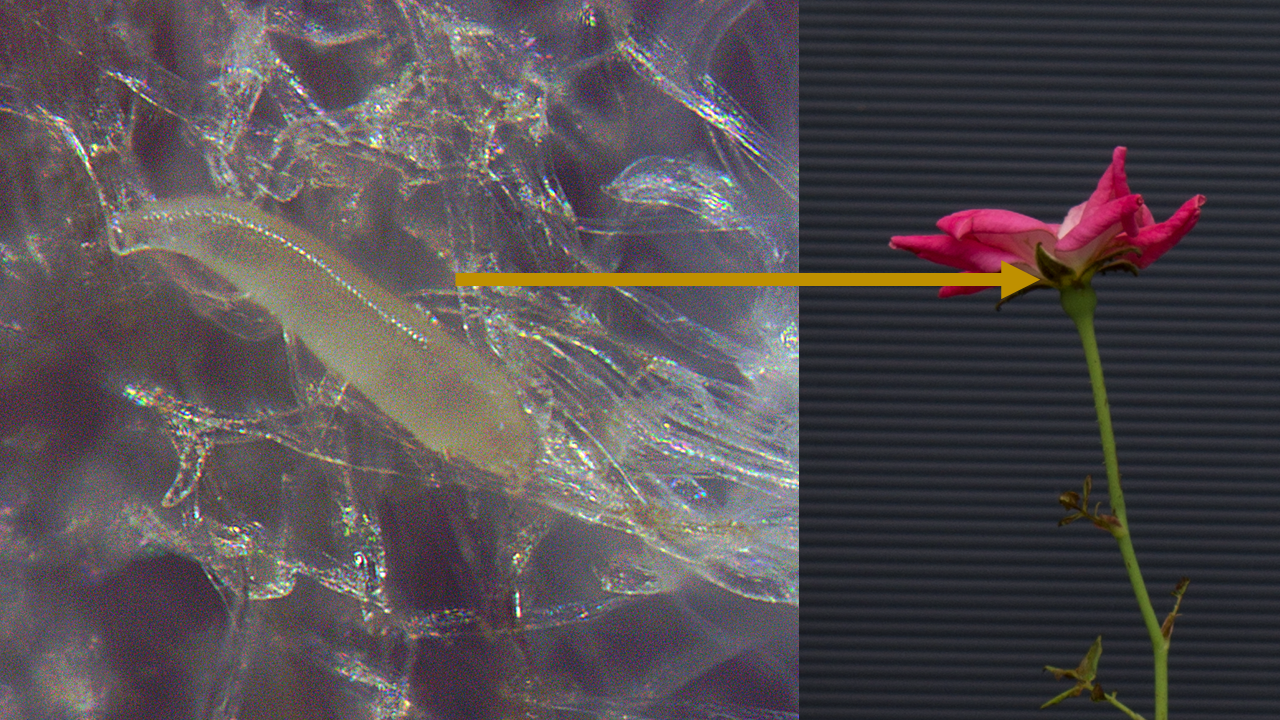
\includegraphics[width=1\linewidth]{figure/mite-pfruct-hide} 

}

\caption[Illustration of the typical location of \textit{Phyllocoptes fructiphilus} on roses.]{Illustration of the typical location of \textit{Phyllocoptes fructiphilus} on roses. \textit{P. fructiphilus} are difficult to manage with pesticides due to the protection offered by the sepals.}\label{fig:hiding}
\end{figure}
\hypertarget{small-phytoseiid-mites-could-be-an-option-for-biocontrol-if-discovered}{%
\subsection{Small phytoseiid mites could be an option for biocontrol if discovered}\label{small-phytoseiid-mites-could-be-an-option-for-biocontrol-if-discovered}}

Eriophyoid mites are hard to control via conventional methods (i.e.~pesticides) due to their small size and their cryptic habits, so alternative methods of pest control are being investigated. There are currently no known natural enemies associated with \emph{P. fructiphilus}, but surveys of eriophyoid-infested plants sometimes encounter predatory mites which may be suitable for biological control (\protect\hyperlink{ref-LawsonBalagbo2007b}{Lawson-Balagbo et al. 2007b}, \protect\hyperlink{ref-Picoli2010}{Picoli et al. 2010}, \protect\hyperlink{ref-Azevedo2016}{Azevedo et al. 2016}). The most well-studied family of predatory is the Phytoseiidae (\protect\hyperlink{ref-Gerson2003}{Gerson et al. 2003}, \protect\hyperlink{ref-Farragut2010}{Farragut et al. 2010}, \protect\hyperlink{ref-Carrillo2015}{Carrillo et al. 2015}), which are sometimes released as biological control agents for thrips, whiteflies, spider mites (Tetranychidae), flat mites (Tenuipalpidae), scale insects and other pests (\protect\hyperlink{ref-Gerson2003}{Gerson et al. 2003}, \protect\hyperlink{ref-Chen2006}{Chen et al. 2006}, \protect\hyperlink{ref-Arthurs2009}{Arthurs et al. 2009}, \protect\hyperlink{ref-Carrillo2011a}{Carrillo et al. 2011a}, \protect\hyperlink{ref-Carrillo2011}{Carrillo and Peña 2011}, \protect\hyperlink{ref-Dogramaci2011}{Doğramaci et al. 2011}, \protect\hyperlink{ref-Sarwar2017}{Sarwar 2017}, \protect\hyperlink{ref-Knapp2018}{Knapp et al. 2018}, \protect\hyperlink{ref-Argolo2020}{Argolo et al. 2020}). Phytoseiid mites are generally associated with plants (\protect\hyperlink{ref-Farragut2010}{Farragut et al. 2010}), and do not survive well without them (\protect\hyperlink{ref-Jung2000}{Jung and Croft 2000}). Plant structures affect many aspects of a phytoseiid's life (\protect\hyperlink{ref-Cortesero2000}{Cortesero et al. 2000}, \protect\hyperlink{ref-Schmidt2013}{Schmidt 2013}), influencing dispersal (\protect\hyperlink{ref-Buitenhuis2013}{Buitenhuis et al. 2013}, \protect\hyperlink{ref-Lopez2016}{Lopez et al. 2016}), as well as performance as predators (\protect\hyperlink{ref-Cedola2001}{Cédola et al. 2001}, \protect\hyperlink{ref-Seelmann2007}{Seelmann et al. 2007}, \protect\hyperlink{ref-Buitenhuis2013}{Buitenhuis et al. 2013}). Some species such as \emph{Neoseiulus paspalivorus} (De Leon) (\protect\hyperlink{ref-LawsonBalagbo2007}{Lawson-Balagbo et al. 2007a}, \protect\hyperlink{ref-Negloh2011}{Negloh et al. 2011}, \protect\hyperlink{ref-Lesna2014}{Lesna et al. 2014}) and \emph{Phytoseius intermedius} Evans \& MacFarlane (\protect\hyperlink{ref-Picoli2010}{Picoli et al. 2010}, \protect\hyperlink{ref-Azevedo2016}{Azevedo et al. 2016}) are small enough that they can feed on refuge-seeking eriophyid mites hiding in difficult to reach areas, such as in erinea or under plant bracts/perianths (\protect\hyperlink{ref-LawsonBalagbo2007a}{Lawson-Balagbo et al. 2007c}, \protect\hyperlink{ref-Azevedo2016}{Azevedo et al. 2016}, \protect\hyperlink{ref-Silva2016}{Silva 2016}). Studies of predatory mites associated with roses can hopefully encounter a similar mite species able to find its way under the sepals, petioles, and glandular plant hairs (trichomes) to feed on hiding \emph{P. fructiphilus} and provide some control (\protect\hyperlink{ref-Howard1991}{Howard and Rodriguez 1991}, \protect\hyperlink{ref-Jesse2006}{Jesse et al. 2006}, \protect\hyperlink{ref-Otero-Colina2018}{Otero-Colina et al. 2018}, \protect\hyperlink{ref-Bauchan2019}{Bauchan et al. 2019}). However, prey-seeking on a large plant is a non-trivial task, accordingly, many species of mites learn to find their hosts or prey by relying on Volatile Organic Compounds (VOCs) to guide them released when plants are injured by pests or infected with pathogens, and use these VOCs to locate their prey (\protect\hyperlink{ref-Sabelis1999}{Sabelis et al. 1999}, \protect\hyperlink{ref-Maeda2001}{Maeda and Takabayashi 2001}, \protect\hyperlink{ref-Boom2002}{Boom et al. 2002}, \protect\hyperlink{ref-Boer2004a}{Boer and Dicke 2004a}, \protect\hyperlink{ref-Boer2004b}{2004b}, \protect\hyperlink{ref-Boer2005}{2005}). The chemistry of VOCs varies depending on plant species, and can create many different effects on the arthropods which inhabit the affected plant: VOCs can repel (\protect\hyperlink{ref-Moraes2001}{Moraes et al. 2001}, \protect\hyperlink{ref-Pichersky2002}{Pichersky and Gershenzon 2002}, \protect\hyperlink{ref-Agut2018}{Agut et al. 2018}) attract (\protect\hyperlink{ref-Nomikou2005}{Nomikou et al. 2005}, \protect\hyperlink{ref-Gadino2012}{Gadino et al. 2012}, \protect\hyperlink{ref-Avellaneda2019}{Avellaneda et al. 2019}), encourage predation (\protect\hyperlink{ref-Kessler2001}{Kessler and Baldwin 2001}, \protect\hyperlink{ref-Halitschke2007}{Halitschke et al. 2007}), or poison arthropods (\protect\hyperlink{ref-Vancanneyt2001}{Vancanneyt et al. 2001}). By manipulating the VOCs which natural enemies or pests encounter on roses, we may be able to inform future research into push-pull strategies (\protect\hyperlink{ref-Cook2007}{Cook et al. 2007}), improve retention of predators at release points, a common issue in mite biocontrol (\protect\hyperlink{ref-Buitenhuis2010}{Buitenhuis et al. 2010}, \protect\hyperlink{ref-Buitenhuis2013}{2013}, \protect\hyperlink{ref-Buitenhuis2015}{2015}).

\hypertarget{chemeco}{%
\section{Induced Plant Defenses - Can Systemic Acquired Resistance Reduce Mite Herbivory?}\label{chemeco}}

Plants are primarily sessile organisms which aren't able to run or hide, therefore undefended plants struggle to grow in the face of the constant threat of herbivory (\protect\hyperlink{ref-Kessler2004}{Kessler et al. 2004}). In order to combat being eaten, plants rely heavily on their ability to protect themselves \emph{in-situ}, via a myriad of different physical and chemical defenses (\protect\hyperlink{ref-Walling2000}{Walling 2000}). These defenses are categorized as either constitutive defenses or induced defenses (\protect\hyperlink{ref-Farmer2016}{Farmer 2016}). Constitutive defenses are always `on', being produced by the plant constantly, such as tannins and latex, while inducible defenses rely on some sort of signal before the plant will produce them. Physical defenses of herbivory includes spines, prickles, thorns, glandular trichomes, latex, sclereids, epicuticular wax, bark, thick cell walls, and compensatory growth to prevent tissue damage while increasing wear on herbivore mouthparts (\protect\hyperlink{ref-Farmer2016}{Farmer 2016}). In addition to these physical barriers to herbivory, plants are also efficient chemical factories which produce a bevy of secondary plant metabolites, including inhibitory proteins, enzymes, and toxins which reduce palatability of plant tissues, prevent uptake of essential amino acids, or kill the herbivore outright (\protect\hyperlink{ref-Farmer2016}{Farmer 2016}). It is hypothesized that inducible defenses must have evolved in response to threats that were sporadic in nature, but strong enough to necessitate a response (\protect\hyperlink{ref-EdelsteinKeshet1989}{Edelstein-Keshet and Rausher 1989}, \protect\hyperlink{ref-Tollrian1999}{Tollrain and Harvell 1999}). The idea is that inducible defenses allow plants a type of cost-saving for their limited resources (Optimal Defense Theory, Steppuhn and Baldwin (\protect\hyperlink{ref-Steppuhn2008}{2008}); Adler and Karban (\protect\hyperlink{ref-Adler1994}{1994})), or to avoid damaging themselves with the compounds used (\protect\hyperlink{ref-Steppuhn2008}{Steppuhn and Baldwin 2008}). Otherwise, the evolution of constitutive defenses would seem to be a better option for plant defense (\protect\hyperlink{ref-Karban1989}{Karban and Myers 1989}, \protect\hyperlink{ref-Jaeremo1999}{Järemo et al. 1999}). A corollary of the optimal defense theory is that inducible defenses should have cues that trigger dependably, accurately and be an effective deterrent once activated, so as to avoid opportunity costs (\protect\hyperlink{ref-Berenbaum1999}{Berenbaum and Zangerl 1999}, \protect\hyperlink{ref-Jaeremo1999}{Järemo et al. 1999}). Induced chemical defenses are thought to have an added benefit of being faster and less costly for plants to produce than other types of defense, such as developing spines or thicker cell walls (\protect\hyperlink{ref-Berenbaum1999}{Berenbaum and Zangerl 1999}, \protect\hyperlink{ref-Jaeremo1999}{Järemo et al. 1999}). Even so, chemical defenses still have drawbacks in allocation costs: plants investing energy into defenses are not using those resources for growth or reproduction (\protect\hyperlink{ref-Berenbaum1999}{Berenbaum and Zangerl 1999}). There are also probably genetic tradeoffs to keep inducible costs active rather than other essential plant functions, and there may be ecological compromises as well: adaptation to one form of defense may preclude the use of another (\protect\hyperlink{ref-Berenbaum1999}{Berenbaum and Zangerl 1999}). Another confounding factor with induced defenses occurs in the presence of specialist herbivores, many of which are especially adapted to overcoming a particular plant defense (\protect\hyperlink{ref-Ehrlich1964}{Ehrlich and Raven 1964}, \protect\hyperlink{ref-Schoonhoven2005}{Schoonhoven et al. 2005}, \protect\hyperlink{ref-Farmer2016}{Farmer 2016}). Järemo et al. (\protect\hyperlink{ref-Jaeremo1999}{1999}) considered the development of systemic responses to be more probable if plant defenses required larger doses for deterrence, and posited that localized responses to herbivory are benefit the plant when small amounts of initial damage are a reliable cues of larger damage to come. This framework readily considers the feeding activities of stylet feeders like mites, whose initial damages are minimal, but quickly accelerate due to mites' fast population growth rates. Accordingly, plants need to be responsive and accurate when identifying a threat before a defense can be mounted. Plants rely on pattern recognition receptors (PRRs) (\protect\hyperlink{ref-Couto2016}{Couto and Zipfel 2016}), to detect pathogen-associated molecular patterns (PAMPS) (\protect\hyperlink{ref-Boller2009}{Boller and Felix 2009}), and herbivore-associated molecular patterns (HAMPS) (\protect\hyperlink{ref-Mithoefer2008}{Mithöfer and Boland 2008}), molecules released from attacking pathogens and herbivores, respectively. These PRRs are part of innate plant immunity: PAMP-triggered immunity and effector-triggered immunity (ETI) (\protect\hyperlink{ref-Chisholm2006}{Chisholm et al. 2006}, \protect\hyperlink{ref-Jones2006}{Jones and Dangl 2006}). Plant cell-surface receptors detect common pathogen molecules, such as flagellar proteins, chitin and ergosterol. If activated PTI typically stops further invasion, by depositing callose at the site of infection, releasing reactive oxygen species (ROS), mitogen-activated protein kinases (MAPK, Howe and Jander (\protect\hyperlink{ref-Howe2008}{2008})), and inducing pathogen-responsive genes. If this first line of defense is surpassed, ETI has evolved to identify the proteins used to overcome PTI, by detecting pathogen effectors with the \emph{R} proteins encoded by the corresponding \emph{R}-genes in the plant (\protect\hyperlink{ref-Boller2009}{Boller and Felix 2009}). One of the most well known effects of activating ETI is the hypersensitive response (HR), rapid localized cell death/necrosis at sites of infection. The HR also activates pathogensis-related (PR) genes and upregulates intercellular Salicylic Acid (SA), which converts to the VOC, Methyl Salicylate (MeSA), a signal which propagates resistance throughout the plant. The increased expression of PR genes primes the plant for resistance to future attacks, via a process known as systemic acquired resistance (SAR) (\protect\hyperlink{ref-Boller2009}{Boller and Felix 2009}, \protect\hyperlink{ref-Vlot2009}{Vlot et al. 2009}, \protect\hyperlink{ref-Zhang2010}{Zhang et al. 2010}). HAMPs work in a similar way to PAMPs, but instead of detecting molecular patterns associated with pathogens, they detect molecules associated with herbivores, such as arthropod oral secretions, eggs, pheromones, or other chemicals conserved across a wide range of arthropods (\protect\hyperlink{ref-Mithoefer2008}{Mithöfer and Boland 2008}). Plants respond to triggered HAMPS in similar ways: they also trigger ROS, MAPKs, and Ca\({^{2+}}\) influx at the site of injury (\protect\hyperlink{ref-Vincent2017}{Vincent et al. 2017}). A second important plant defense is the Jasmonic Acid (JA)-Ethylene (ET) signalling pathways. The JA/ET pathways are activated when JA upregulates in response to wounding and/or arthropod damage, and provides protection from herbivory as well as pathogen damage (\protect\hyperlink{ref-Thaler2001}{Thaler et al. 2001}, \protect\hyperlink{ref-Farmer2003}{Farmer et al. 2003}, \protect\hyperlink{ref-Guo2004}{Guo and Ecker 2004}, \protect\hyperlink{ref-Glazebrook2005}{Glazebrook 2005}, \protect\hyperlink{ref-Howe2008}{Howe and Jander 2008}). Plants can be primed directly through application of SA, MeSA or even synthetic chemical analogues, such as acibenzolar-S-methyl (ASM) to activate SAR (\protect\hyperlink{ref-Anfoka2000}{Anfoka 2000}, \protect\hyperlink{ref-Conrath2006}{Conrath et al. 2006}, \protect\hyperlink{ref-Vlot2009}{Vlot et al. 2009}, \protect\hyperlink{ref-Zhang2010}{Zhang et al. 2010}, \protect\hyperlink{ref-Jeschke2015}{Jeschke 2015}). Exogenous applications of ASM can protect plants in the same way as SA applications, by activating the SAR pathway, reducing disease incidence and severity of pathogenic fungi (\protect\hyperlink{ref-Ziadi2001}{Ziadi et al. 2001}, \protect\hyperlink{ref-Tripathi2010}{Tripathi et al. 2010}, \protect\hyperlink{ref-Jeschke2015}{Jeschke 2015}), bacteria (\protect\hyperlink{ref-Romero2001}{Romero et al. 2001}), phytoplasmas (\protect\hyperlink{ref-Ratchaseema2021}{Ratchaseema et al. 2021}), and viruses (\protect\hyperlink{ref-Anfoka2000}{Anfoka 2000}, \protect\hyperlink{ref-Babu2021}{Babu et al. 2021}, \protect\hyperlink{ref-Doungous2021}{Doungous et al. 2021}). ASM application (SAR-induction) has also been noted for its ability to promote wound healing in potatoes (\protect\hyperlink{ref-Jiang2019}{Jiang et al. 2019}), and control whiteflies (\protect\hyperlink{ref-Correa2005}{Correa et al. 2005}, \protect\hyperlink{ref-Doungous2021}{Doungous et al. 2021}) as well as aphids (\protect\hyperlink{ref-Costa2006}{Costa and Moraes 2006}). Taken together, induced plant defenses offer an important potential role in the prevention of disease and control of insect pests.

\hypertarget{effects-of-systemic-acquired-resistance-on-eriophyoid-mites}{%
\subsection{Effects of Systemic Acquired Resistance on eriophyoid mites}\label{effects-of-systemic-acquired-resistance-on-eriophyoid-mites}}

Induced plant defenses have been studied somewhat for their effects on eriophyoid and other herbivorous mites: Bronner et al. (\protect\hyperlink{ref-Bronner1991}{1991a}), Bronner et al. (\protect\hyperlink{ref-Bronner1991a}{1991b}), Westphal et al. (\protect\hyperlink{ref-Westphal1991}{1991}), and Westphal et al. (\protect\hyperlink{ref-Westphal1992}{1992}) observed that feeding by the gall mite \emph{Aceria cladophthirus} (Nalepa) activated induced defenses, triggering the hypersensitive response in \emph{Solanum dulcamara}. As part of SAR-induction these plants increased their levels of \textbeta-1,3-glucanase and chitinases (\protect\hyperlink{ref-Bronner1991a}{Bronner et al. 1991b}, \protect\hyperlink{ref-Ward1991a}{Ward et al. 1991}, \protect\hyperlink{ref-Bhardwaj2021}{Bhardwaj et al. 2021}), enzymes which together help to prevent fungal disease development (\protect\hyperlink{ref-Mauch1984}{Mauch et al. 1984}, \protect\hyperlink{ref-Mauch1988}{1988}, \protect\hyperlink{ref-Goy1992}{Goy et al. 1992}, \protect\hyperlink{ref-Xue1998}{Xue et al. 1998}, \protect\hyperlink{ref-Narusaka1999}{Narusaka et al. 1999}, \protect\hyperlink{ref-Suo2001}{Suo and Leung 2001}, \protect\hyperlink{ref-AnguelovaMerhar2008}{Anguelova-Merhar et al. 2008}, \protect\hyperlink{ref-Bhardwaj2021}{Bhardwaj et al. 2021}, \protect\hyperlink{ref-Rajninec2021}{Rajninec et al. 2021}). Similar responses have been seen in grapes (Vitis vinifera L.) attacked by the erineum mite \emph{Colomerus vitis} Pagenstecher (\protect\hyperlink{ref-Khederi2018b}{Khederi et al. 2018a}), at least suggesting that the SAR-induction is not solely limited to the Solanaceae, and likely occurs in many eriophyid-plant systems. Induced plant defenses show promise for interfering with establishment of these mites: Experiments by Westphal et al. (\protect\hyperlink{ref-Westphal1991}{1991}) found that \emph{S. dulcamara}'s SAR response to \emph{A. cladophthirus} produced 40-day protection from subsequent colonization by more \emph{A. cladophthirus} or another eriophyid, \emph{Thamnacus solani} Boczek and Michalska, a rust mite. Westphal et al. (\protect\hyperlink{ref-Westphal1992}{1992}) continued to demonstrate that these induced responses were not enough not protect the plant from \emph{Tetranychus urticae} Koch, but instead increased their fecundity, possibly due to negative cross-talk between SA and JA that is found in some plant systems (\protect\hyperlink{ref-Baldwin1997}{Baldwin et al. 1997}, \protect\hyperlink{ref-Belliure2010}{Belliure et al. 2010}, \protect\hyperlink{ref-Thaler2012}{Thaler et al. 2012}). For example, Warabieda et al. (\protect\hyperlink{ref-Warabieda2020}{2020}) observed that JA helped increase plant resistance to \emph{T. urticae}, but applying JA and ASM together was less effective than applying JA alone, due to SA interference with JA pathways. Other studies have found opposite effects: Favaro et al. (\protect\hyperlink{ref-Favaro2019}{2019}) reported reduced numbers of \emph{T. urticae} on strawberries post SA induction, and Khederi et al. (\protect\hyperlink{ref-Khederi2018}{2018b}) found that SA and JA induction was sufficient to control erineum forming \emph{Colomerus vitis} (Pagenstecher). David et al. (\protect\hyperlink{ref-David2021}{2021}) showed how damage from chewing herbivores and exogenous applications of JA reduced gall formation, but did not significantly reduce populations of the eriophyid mite, \emph{Floracarus perrepae} Knihinicki and Boczek (\protect\hyperlink{ref-David2021}{David et al. 2021}). This type of inconsistency is best explained by the results of Kant et al. (\protect\hyperlink{ref-Kant2007}{2007}), which found examples of interspecific variation of \emph{T. urticae}'s ability to induce--and resist--JA defenses. Furthermore, there have been a number of cases where mites have been known to avoid or prevent upregulation of plant defenses entirely: Both \emph{T. urticae} and \emph{Aculops lycopersici} Massee, have been reported to suppress the JA pathways without relying on antagonistic cross-talk between the responses (\protect\hyperlink{ref-Sarmento2011}{Sarmento et al. 2011}, \protect\hyperlink{ref-Alba2014}{Alba et al. 2014}), instead by suppressing downstream accumulation of JA (\protect\hyperlink{ref-Alba2014}{Alba et al. 2014}, \protect\hyperlink{ref-Glas2014}{Glas et al. 2014}). Glas et al. (\protect\hyperlink{ref-Glas2014}{2014}) observed that \emph{A. lycopersici} would still induces SA defenses, while an inducer species (\protect\hyperlink{ref-Kant2007}{Kant et al. 2007}) of \emph{T. urticae} feeding on tomato (\emph{Solanum lycopersicum}) induces both JA and SA pathways, but when both mites were introduced to the same plant, the JA response plummeted and SA doubled (\protect\hyperlink{ref-Glas2014}{Glas et al. 2014}). This caused \emph{A. lycopersici} populations to suffer while the \emph{T. urticae} populations benefited from \emph{A. lycopersici}'s reduction of JA (\protect\hyperlink{ref-Glas2014}{Glas et al. 2014}). Vectors of plant pathogens create a similar struggle for their host plants by manipulating and suppressing the SA and JA/ET pathways for their mutual benefits (\protect\hyperlink{ref-Agrawal1999}{Agrawal and Karban 1999}, \protect\hyperlink{ref-Belliure2010}{Belliure et al. 2010}). An example can be seen in the interactions of \emph{B. yothersi}, the vector of \emph{Citrus leprosis virus C} (CiLV-C): infection of \emph{Arabidopsis thaliana} and \emph{Citrus} species with CiLV-C induces SA and suppresses JA/ET pathways through crosstalk (\protect\hyperlink{ref-Arena2016}{Arena et al. 2016}). Another study of \emph{B. yothersi} feeding on \emph{A. thaliana} was similar in result: mite feeding triggered both SA and JA/ET pathways, but \emph{B. yothersi} reared on mutant \emph{A. thaliana} with no SA response had lower fecundity (\protect\hyperlink{ref-Arena2018}{Arena et al. 2018}), suggesting that \emph{B. yothersi} rely on inducing SA to antagonize JA production. Inducing plant defenses can have negative consequences for the predators as well as the herbivores present in the system (\protect\hyperlink{ref-Pappas2017}{Pappas et al. 2017}): Ataide et al. (\protect\hyperlink{ref-Ataide2016}{2016}) observed that inducing a plant JA pathway reduced \emph{T. urticae} and \emph{T. evansi} mite performance, but also negatively affected ovophagy by \emph{Phytoseiulus longipes}, which ate fewer eggs from mites living on induced plants (\protect\hyperlink{ref-Ataide2016}{Ataide et al. 2016}), slowing their reproductive rate. It is also possible that the differences feeding methods between mite species is creating different defense responses, as has been seen in other arthropod groups (\protect\hyperlink{ref-Zarate2006}{Zarate et al. 2006}, \protect\hyperlink{ref-Zhang2009}{Zhang et al. 2009}, \protect\hyperlink{ref-Arimura2011}{Arimura et al. 2011}). In conclusion, this type of interplay between induced defenses is common, sometimes host-specific, and can vary by plant species or cultivar (\protect\hyperlink{ref-Boom2004}{Boom et al. 2004}, \protect\hyperlink{ref-AnguelovaMerhar2008}{Anguelova-Merhar et al. 2008}, \protect\hyperlink{ref-Petanovic2010}{Petanović and Kielkiewicz 2010a}). Plant defensive responses also change across life stages (\protect\hyperlink{ref-Sobral2021}{Sobral et al. 2021}), meaning that plant-pathogen-arthropod system should carefully examined mechanistically to better understand the multitrophic interactions at play (\protect\hyperlink{ref-Turlings2018}{Turlings and Erb 2018}).

\hypertarget{improving-the-staying-power-of-biological-control-why-are-amblyseius-swirskii-leaving-rose-patches}{%
\subsection{\texorpdfstring{Improving the staying power of biological control: Why are \emph{Amblyseius swirskii} leaving rose patches?}{Improving the staying power of biological control: Why are Amblyseius swirskii leaving rose patches?}}\label{improving-the-staying-power-of-biological-control-why-are-amblyseius-swirskii-leaving-rose-patches}}

One of the more popular species of commercially-available predatory mite is \emph{Amblyseius swirskii} Athias-Henriot (\protect\hyperlink{ref-Calvo2014}{Calvo et al. 2014}). \emph{A. swirskii} tolerate shipping well (\protect\hyperlink{ref-Lopez2016a}{Lopez and Smith 2016}) and are often sold packaged in vermiculite or in sachets with wheat bran which allows the mites to slowly release into the environment (\protect\hyperlink{ref-Buitenhuis2014}{Buitenhuis et al. 2014}, \protect\hyperlink{ref-Calvo2014}{Calvo et al. 2014}, \protect\hyperlink{ref-Addesso2018}{Addesso et al. 2018}). \emph{A. swirskii} do not feed on leaves (\protect\hyperlink{ref-Nomikou2003}{Nomikou et al. 2003}), and are considered a generalist predator capable of surviving on artificial diets (\protect\hyperlink{ref-Nguyen2013}{Nguyen et al. 2013}), natural or supplemental pollen (\protect\hyperlink{ref-Loughner2011}{Loughner et al. 2011}, \protect\hyperlink{ref-Park2011}{Park et al. 2011}, \protect\hyperlink{ref-Delisle2015}{Delisle et al. 2015}, \protect\hyperlink{ref-Ghasemzadeh2017}{Ghasemzadeh et al. 2017}), or a variety of other microarthropods present in the natural environment (\protect\hyperlink{ref-Janssen2015}{Janssen and Sabelis 2015}, \protect\hyperlink{ref-Kumar2015}{Kumar et al. 2015}). Furthermore, \emph{A. swirskii} have been tested for their compatibility with various combinations of other biocontrol agents, such as predatory mirids, minute pirate bugs, and \emph{Beauveria bassiana} (\protect\hyperlink{ref-Chow2010}{Chow et al. 2010}, \protect\hyperlink{ref-Midthassel2016}{Midthassel et al. 2016}, \protect\hyperlink{ref-Bouagga2018}{Bouagga et al. 2018}). Certain modern pesticides and reduced risk-fungicides had relatively low toxicity to \emph{A. swirskii} while other agrichemicals increase mortality or reduce fecundity (\protect\hyperlink{ref-Gradish2010}{Gradish et al. 2010}, \protect\hyperlink{ref-Masui2014}{Masui et al. 2014}, \protect\hyperlink{ref-Fernandez2017}{Fernández et al. 2017}, \protect\hyperlink{ref-Ersin2020}{Ersin et al. 2020}, \protect\hyperlink{ref-Havasi2021}{Havasi et al. 2021}). Agrichemical products should be tested for their compatibility with biocontrol agents before they are utilized in a pest management program. \emph{A. swirskii} have been used to control a variety of pests on greenhouse vegetable crops, including thrips (\protect\hyperlink{ref-Calvo2007}{Calvo and Belda 2007}, \protect\hyperlink{ref-Messelink2008}{Messelink et al. 2008}, \protect\hyperlink{ref-Arthurs2009}{Arthurs et al. 2009}, \protect\hyperlink{ref-Calvo2010}{Calvo et al. 2010}), whiteflies (\protect\hyperlink{ref-Nomikou2001}{Nomikou et al. 2001}, \protect\hyperlink{ref-Nomikou2002}{Nomikou et al. 2002}, \protect\hyperlink{ref-Calvo2007}{Calvo and Belda 2007}, \protect\hyperlink{ref-Messelink2008}{Messelink et al. 2008}, \protect\hyperlink{ref-Calvo2010}{Calvo et al. 2010}), \emph{Polyphagotarsonemus latus} (Banks) (\protect\hyperlink{ref-Maanen2010}{Maanen et al. 2010}, \protect\hyperlink{ref-Onzo2012}{Onzo et al. 2012}), and to a lesser extent, \emph{T. urticae} (\protect\hyperlink{ref-Momen1993}{Momen and Elsaway 1993}, \protect\hyperlink{ref-Messelink2009}{Messelink et al. 2009}, \protect\hyperlink{ref-Xu2010}{Xu and Enkegaard 2010}). It is difficult for \emph{A. swirskii} to enter into the webbing of \emph{T. urticae} (\protect\hyperlink{ref-Messelink2009}{Messelink et al. 2009}), and when given the choice between \emph{Frankliniella occidentalis} (Pergande) and \emph{T. urticae} as prey, about twice as many \emph{F. occidentalis} were eaten (\protect\hyperlink{ref-Xu2010}{Xu and Enkegaard 2010}). Although \emph{A. swirskii} apparently do not prefer \emph{T. urticae} they have been reported to feed on eriophyid mites: Momen and Abdel-Khalek (\protect\hyperlink{ref-Momen2008}{2008}) found high fecundity and net reproductive rate for \emph{A. swirskii} feeding on \emph{Aculops lycopersici} (Massee), and Momen and Elsaway (\protect\hyperlink{ref-Momen1993}{1993}) reported faster reproduction and development when \emph{A. swirskii} fed on \emph{Eriophyes dioscoridis} Soliman and Abou-Awad. The same study reported that \emph{A. swirskii} preferred \emph{A. lycopersici} over either \emph{T. urticae} or castor bean pollen \emph{Ricinus communis} (L.). Similarly, Park et al. (\protect\hyperlink{ref-Park2010}{2010}) showed increased oviposition and reproductive rates for \emph{A. swirskii} feeding on \emph{A. lycopersici}. They also saw more feeding on \emph{A. lycopersici} than cattail (\emph{Typha latifolia} {[}L.{]}) pollen, and very slight preference for \emph{A. lycopersici} feeding over the common thrips species they had present in their study (\emph{F. occidentalis} and \emph{Thrips tabaci} Lindeman) (\protect\hyperlink{ref-Park2011}{Park et al. 2011}). Although the aforementioned thrips, whiteflies and mites are serious pests of ornamental greenhouse crops, predatory mites such as \emph{A. swirskii} are seldom used (\protect\hyperlink{ref-Buitenhuis2015}{Buitenhuis et al. 2015}). A number of studies have tested \emph{A. swirskii} in roses for their suitability to control thrips, greenhouse whitefly and \emph{T. urticae} (\protect\hyperlink{ref-Chow2010}{Chow et al. 2010}, \protect\hyperlink{ref-Hoogerbrugge2011}{Hoogerbrugge et al. 2011}, \protect\hyperlink{ref-Hoogerbrugge2014}{Hoogerbrugge et al. 2014}, \protect\hyperlink{ref-Alipour2016}{Alipour et al. 2016}, \protect\hyperlink{ref-Alipour2019}{2019}, \protect\hyperlink{ref-Houten2016}{Houten et al. 2016}), but has been little adoption of biocontrol by growers in ornamental crops (\protect\hyperlink{ref-Buitenhuis2015}{Buitenhuis et al. 2015}), or crops in general (\protect\hyperlink{ref-Lenteren2011}{Lenteren 2011}). Even so, there is increasing interest by some growers to implement biological control into their greenhouse production systems (\protect\hyperlink{ref-Buitenhuis2015}{Buitenhuis et al. 2015}). Unfortunately, in some releases of \emph{A. swirskii} in roses, growers felt that the mites were not effective control of \emph{Scirtothrips dorsalis} Hood (\protect\hyperlink{ref-Schoeller2020}{Schoeller et al. 2020}), an unexpected outcome for a mite known to feed on many species of thrips, as previously mentioned. Schoeller et al. (\protect\hyperlink{ref-Schoeller2020}{2020}) hypothesizes that this reduction in thrips control may be due to reduced trichomes on roses. This hypothesis agrees with the reports of Loughner et al. (\protect\hyperlink{ref-Loughner2010}{2010a}) and Loughner et al. (\protect\hyperlink{ref-Loughner2010a}{2010b}), who noted that phytoseiids tend to disperse away from plants with few trichomes. Even so, phytoseiids tend to oviposit on dense patches of trichomes along axillary veins known as `domatia' on the underside of leaves (\protect\hyperlink{ref-ODowd1991}{O'Dowd and Willson 1991}, \protect\hyperlink{ref-Walter1992}{Walter 1992}, \protect\hyperlink{ref-Walter1996}{1996}, \protect\hyperlink{ref-Grostal1994}{Grostal and O'Dowd 1994}, \protect\hyperlink{ref-Agrawal1997}{Agrawal and Karban 1997}), a behavior which is thought to help to avoid predation (\protect\hyperlink{ref-Faraji2002}{Faraji et al. 2002}), so it is unclear if phytoseiids leaving roses is simply due to having few trichomes. Also, the idea that \emph{A. swirskii} dislike glabrous surfaces contrasts with McMurtry et al. (\protect\hyperlink{ref-McMurtry2013}{2013})'s classification of \emph{A. swirskii} as a type III-b phytoseiid mite: a generalist predator which lives on glabrous surfaces. This classification was recently challenged by Liu et al. (\protect\hyperlink{ref-Liu2017}{2017}), who recovered only three feeding guilds of phytoseiids from detailed analysis of morphometric data. Liu et al. (\protect\hyperlink{ref-Liu2017}{2017})'s results were more similar to earlier classifications McMurtry and Croft (\protect\hyperlink{ref-McMurtry1997}{1997}), which had separated the phytoseiids into three feeding groups: specialists of \emph{Tetranychus} species (type I), generalist predators (type II), and \emph{Euseius utilis}, a pollen feeding phytoseiid (type III) (\protect\hyperlink{ref-McMurtry1997}{McMurtry and Croft 1997}, \protect\hyperlink{ref-McMurtry2013}{McMurtry et al. 2013}, \protect\hyperlink{ref-Liu2017}{Liu et al. 2017}). Even if \emph{A. swirskii}'s preference for glabrous habitats is in question, there are other concerns with utilizing them for biological control of roses. Experiments with \emph{T. urticae}-resistant roses revealed some issues when combining \emph{A. swirskii} with another common predator of \emph{T. urticae}, \emph{Phytoseiulus persimilis} Athias-Henriot (\protect\hyperlink{ref-Alipour2016}{Alipour et al. 2016}, \protect\hyperlink{ref-Alipour2019}{2019}). Alipour et al. (\protect\hyperlink{ref-Alipour2016}{2016}) saw that predators fed more on \emph{T. urticae} on the resistant rose cultivar, but \emph{P. persimilis} generally outperformed \emph{A. swirskii}, with higher predation rates. This study seems to simply reaffirm prior knowledge about the feeding preferences of these mite species on \emph{T. urticae}, but a follow-up study in 2019 found some antagonistic effects on the intrinsic rate of increase for both predators as well as \emph{T. urticae} on the resistant roses (\protect\hyperlink{ref-Alipour2019}{Alipour et al. 2019}). These effects may be due to host plant resistance (antibiosis), or possibly induced plant defenses (\protect\hyperlink{ref-Stout2013}{Stout 2013}) caused by \emph{T. urticae} feeding. These types of plant defense mechanisms have have potential to help control mites such as \emph{T. urticae} (\protect\hyperlink{ref-Agut2018}{Agut et al. 2018}), but as demonstrated by the example of Alipour et al. (\protect\hyperlink{ref-Alipour2019}{2019}), the mechanisms of host plant resistance must be closely examined to avoid harming beneficial organisms in the same plant system (\protect\hyperlink{ref-Pappas2017}{Pappas et al. 2017}).

\hypertarget{a-second-plant-mite-pathosystem-brevipalpus-californicus-and-orchid-fleck-dichorhavirus}{%
\section{\texorpdfstring{A Second Plant-Mite-Pathosystem: \emph{Brevipalpus californicus} and \emph{Orchid fleck dichorhavirus}}{A Second Plant-Mite-Pathosystem: Brevipalpus californicus and Orchid fleck dichorhavirus}}\label{a-second-plant-mite-pathosystem-brevipalpus-californicus-and-orchid-fleck-dichorhavirus}}

The most important superfamily of herbivorous mites is the Tetranychoidea. The Tetranychoidea are comprised of 2,000 species divided into 5 families (\protect\hyperlink{ref-Krantz2009}{Krantz 2009}), two of which have economic significance, Tetranychidae--the spider mites--and Tenuipalpidae. Tenuipalpidae are known colloquially as the false spider mites, or flat mites due to their flattened character and superficial similarity to the Tetranychidae. In contrast to tetranychids, tenuipalpids do not spin webs and are considered to be a pest of reduced severity: Krantz (\protect\hyperlink{ref-Krantz2009}{2009}) places them as the `third most important family of phytophagous mites'. Flat mites are considered to be a tropical to subtropical group of mites (\protect\hyperlink{ref-Gerson2008}{Gerson 2008}), the majority of which are not of economic significance (\protect\hyperlink{ref-Hoy2011}{Hoy 2011}). Consequently, tenuipalpids have been studied much less than the Tetranychidae (\protect\hyperlink{ref-Jeppson1975}{Jeppson et al. 1975b}, \protect\hyperlink{ref-Childers2003b}{Childers et al. 2003a}, \protect\hyperlink{ref-Gerson2008}{Gerson 2008}), but flat mites from the genus \emph{Brevipalpus} have been gaining importance in recent years as vectors of plant viruses (\protect\hyperlink{ref-Chagas2003}{Chagas et al. 2003}, \protect\hyperlink{ref-Childers2003a}{Childers et al. 2003c}, \protect\hyperlink{ref-Childers2003c}{Childers and Derrick 2003}, \protect\hyperlink{ref-Kitajima2003b}{Kitajima et al. 2003}, \protect\hyperlink{ref-Rodrigues2003a}{Rodrigues et al. 2003}, \protect\hyperlink{ref-Kitajima2008}{Kitajima et al. 2008}, \protect\hyperlink{ref-Kitajima2010}{2010}, \protect\hyperlink{ref-Childers2011}{Childers and Rodrigues 2011}, \protect\hyperlink{ref-Melzer2013}{Melzer et al. 2013}, \protect\hyperlink{ref-Rodrigues2013}{Rodrigues and Childers 2013}, \protect\hyperlink{ref-RamosGonzalez2017}{Ramos-González et al. 2017}, \protect\hyperlink{ref-ChabiJesus2018}{Chabi-Jesus et al. 2018}, \protect\hyperlink{ref-Dietzgen2018}{Dietzgen et al. 2018a}). Another major pest of modern concern is \emph{Raoiella indica} (Hirst), a pest of palms (Arecaceae), ginger (Zingiberaceae), bananas (Musaceae), and bird of paradise plants (Strelitziaceae) (\protect\hyperlink{ref-Jeppson1975}{Jeppson et al. 1975b}, \protect\hyperlink{ref-Etienne2006}{Etienne and Flechtmann 2006}, \protect\hyperlink{ref-Hoy2011}{Hoy 2011}, \protect\hyperlink{ref-Beard2012a}{Beard et al. 2012}), which has been invading the Neotropics since their introduction to the Caribbean (\protect\hyperlink{ref-Etienne2006}{Etienne and Flechtmann 2006}, \protect\hyperlink{ref-Rodrigues2007}{Rodrigues et al. 2007}, \protect\hyperlink{ref-Roda2008}{Roda et al. 2008}, \protect\hyperlink{ref-Vasquez2008}{Vásquez et al. 2008}, \protect\hyperlink{ref-Carrillo2011b}{Carrillo et al. 2011b}, \protect\hyperlink{ref-Dowling2011}{Dowling et al. 2011}, \protect\hyperlink{ref-Kane2012}{Kane et al. 2012}, \protect\hyperlink{ref-Pena2012}{Peña et al. 2012}, \protect\hyperlink{ref-Alcivar2020}{Alcı́var et al. 2020}, \protect\hyperlink{ref-EscobarGarcia2020}{Escobar-Garcia and Andrade 2020}, \protect\hyperlink{ref-Ramirez2020}{Ramı́rez et al. 2020}, \protect\hyperlink{ref-Rodrigues2020}{Rodrigues et al. 2020}, \protect\hyperlink{ref-Amaro2021}{Amaro et al. 2021}). Flat mites are typically small (200 to 300 \si{\micro\metre}) red or green, and move slowly (\protect\hyperlink{ref-Jeppson1975}{Jeppson et al. 1975b}, \protect\hyperlink{ref-Hoy2011}{Hoy 2011}). Tenuipalpids feeding is typically restricted to a few hosts, and mites can usually be found on the underside of leaves, often along leaf veins or the midrib (\protect\hyperlink{ref-Jeppson1975}{Jeppson et al. 1975b}, \protect\hyperlink{ref-Hoy2011}{Hoy 2011}). Some species feed on grass, bark, flower heads, leaf sheaths, or form galls (\protect\hyperlink{ref-Jeppson1975}{Jeppson et al. 1975b}, \protect\hyperlink{ref-Hoy2011}{Hoy 2011}). Flat mites have egg, larva, protonymph, deutonymph and adult forms over an average of 3-4 weeks (\protect\hyperlink{ref-Hoy2011}{Hoy 2011}). A few species have only six legs as adults. Tenuipalpid mites can be difficult to classify correctly with light microscopy, due to distortions during mounting of characters used in species identification (\protect\hyperlink{ref-Welbourn2003}{Welbourn et al. 2003}). Furthermore, flat mites are thelytokous parthenogenic: Males are seldom encountered, due to infections with the feminizing bacteria \emph{Candidatus} Cardinium (Cytophaga--Flavobacterium--Bacteroides phylum) Chigira and Miura (\protect\hyperlink{ref-Chigira2005}{2005}). This has caused some concern that some \emph{Brevipalpus} species are actually isofemale lines specialized on their specific hosts (\protect\hyperlink{ref-Groot2005}{Groot et al. 2005}), an idea which is further complicated by the occurrence of cryptic species in these groups (\protect\hyperlink{ref-Navia2013}{Navia et al. 2013}, \protect\hyperlink{ref-Skoracka2015}{Skoracka et al. 2015}). Few methods of pest management have been reported from past reviews of tenuipalpids (\protect\hyperlink{ref-Jeppson1975}{Jeppson et al. 1975b}, \protect\hyperlink{ref-Gerson2008}{Gerson 2008}, \protect\hyperlink{ref-Hoy2011}{Hoy 2011}): a number of different mite predators have been tested for their efficacy, as well as the pathogenic fungi \emph{Hirsutella thompsonii} and \emph{Metarhizium anisopliae} (\protect\hyperlink{ref-RossiZalaf2006}{Rossi-Zalaf and Alves 2006}, \protect\hyperlink{ref-Gerson2008}{Gerson 2008}). Zheng et al. (\protect\hyperlink{ref-Zheng2012}{2012}) tested the ability of water and phytoseiids to reduce populations of \emph{B. obovatus}. \emph{Beauveria bassiana} has been tested to control \emph{R. indica}, and is potentially compatible with the previously-tested phytoseiid species \emph{Amblyseius largoensis} and \emph{Typhlodromus ornatus} (\protect\hyperlink{ref-Carrillo2011}{Carrillo and Peña 2011}, \protect\hyperlink{ref-Freitas2021}{Freitas et al. 2021}). Chemical applications are typically used to control tenuipalpids (\protect\hyperlink{ref-Childers1994}{Childers 1994}), but some species have begun to develop chemical resistance to the more common applications (\protect\hyperlink{ref-Campos2002}{Campos and Omoto 2002}, \protect\hyperlink{ref-Rocha2021}{Rocha et al. 2021}).
\begin{figure}

{\centering \includegraphics[width=1\linewidth]{thesis_files/figure-latex/brevi-fungus-1} 

}

\caption[Cryo-SEM image of Tenuipalpid mite infected with unidentified fungus]{a) Cryo-SEM image of Tenuipalpid mite infected with unidentified fungus, collected from \textit{Liriope muscari}. Arrow indicates sporangia seen enlargement b) detail of sporangia. Photo Credit: Dr. Gary R. Bauchan, USDA-ARS, 2020}\label{fig:brevi-fungus}
\end{figure}
One of the more cosmopolitan species of tenuipalpid is \emph{Brevipalpus californicus} (Banks). \emph{B. californicus} is a common pest with a large host range of agricultural and ornamental crops, including tea, orchids, citrus, cotton and tobacco (\protect\hyperlink{ref-Jeppson1975}{Jeppson et al. 1975b}, \protect\hyperlink{ref-Hoy2011}{Hoy 2011}). \emph{B. californicus} acts as the primary vector for Orchid fleck dichorhavirus (OFV), the type member for the genus \emph{Dichorhavirus}, family \emph{Rhabdoviridae}; a bacilliform, nuclear rhabdoviruses composed of two segments of single-stranded, negative-sense RNA which infects plants (\protect\hyperlink{ref-Dietzgen2014}{Dietzgen et al. 2014}, \protect\hyperlink{ref-Walker2018}{Walker et al. 2018}, \protect\hyperlink{ref-Amarasinghe2019}{Amarasinghe et al. 2019}). Dichorhaviruses are only known to be transmitted by mites in the genus \emph{Brevipalpus} (\protect\hyperlink{ref-Dietzgen2014}{Dietzgen et al. 2014}). Other members of this genus are: Citrus chlorotic spot virus, Citrus leprosis virus N, Clerodendrum chlorotic spot virus and Coffee ringspot virus (\protect\hyperlink{ref-Dietzgen2018}{Dietzgen et al. 2018a}). Many orchid genera are able to become infected with OFV (\protect\hyperlink{ref-Kondo2006}{Kondo et al. 2006}, \protect\hyperlink{ref-Kondo2006}{2006}), as well as some Asparagaceae (Nolinoidaea) (\protect\hyperlink{ref-Dietzgen2018}{Dietzgen et al. 2018a}), and \emph{Citrus} plants (Rutaceae), where it causes leprosis-like symptoms (\protect\hyperlink{ref-Bastianel2010}{Bastianel et al. 2010}, \protect\hyperlink{ref-Roy2013a}{Roy et al. 2013}, \protect\hyperlink{ref-GarciaEscamilla2018}{García-Escamilla et al. 2018}). Mechanical transmission of OFV is possible under lab conditions to various Chenopodiaceae, Aizoaceae, Fabaceae, and Solanaceae (\protect\hyperlink{ref-Chang1976}{Chang et al. 1976}, \protect\hyperlink{ref-Kondo2003}{Kondo et al. 2003}, \protect\hyperlink{ref-Peng2013}{Peng et al. 2013}). \emph{B. californicus} has been collected from OFV-infected Nolinoidaea plants in Australia (\protect\hyperlink{ref-Mei2016}{Mei et al. 2016}, \protect\hyperlink{ref-Dietzgen2018a}{Dietzgen et al. 2018b}). \emph{B. californicus} was historically associated with cases of citrus leprosis disease of Florida and Texas prior to 1925, when the disease mysteriously disappeared from the US sometime during the 1960s (\protect\hyperlink{ref-Knorr1968b}{Knorr et al. 1968}, \protect\hyperlink{ref-Childers2003}{Childers et al. 2003b}). Later studies of herbarium specimens from this time period revealed this disease to be caused by a Dichorhavirus, distantly related to modern OFV strains (\protect\hyperlink{ref-Kitajima2011a}{Kitajima et al. 2011}, \protect\hyperlink{ref-Hartung2015}{Hartung et al. 2015}). Maeda (\protect\hyperlink{ref-Maeda1998}{1998}) found evidence that \emph{B. californicus} can transmit OFV in a persistent propagative manner, which means that the virus may replicate inside of its mite vector. OFV was first described infecting \emph{Cymbidium} orchids in Japan (\protect\hyperlink{ref-Doi1977}{Doi et al. 1977}). Many countries have reported OFV and OFV-like rhabdoviruses infecting orchids worldwide (\protect\hyperlink{ref-Kondo2003}{Kondo et al. 2003}), including Asia: {[}China (\protect\hyperlink{ref-Peng2017}{Peng et al. 2017}), Korea (\protect\hyperlink{ref-Peng2013}{Peng et al. 2013}){]}, Africa: {[}South Africa (\protect\hyperlink{ref-Blanchfield2001}{Blanchfield et al. 2001}, \protect\hyperlink{ref-Cook2019}{Cook et al. 2019}), North America: {[}The US (\protect\hyperlink{ref-Blanchfield2001}{Blanchfield et al. 2001}), (\protect\hyperlink{ref-Bratsch2015}{Bratsch et al. 2015}){]}, South America: {[}Brazil Kitajima et al. (\protect\hyperlink{ref-Kitajima2001}{2001}), Colombia (\protect\hyperlink{ref-Kubo2009}{Kubo et al. 2009b}), Costa Rica (\protect\hyperlink{ref-FreitasAstua2002}{Freitas-Astúa et al. 2002}), Paraguay (\protect\hyperlink{ref-RamosGonzalez2015}{Ramos-González et al. 2015}), Europe: (\protect\hyperlink{ref-Begtrup1972}{Begtrup 1972}), Germany (\protect\hyperlink{ref-Petzold1971}{Petzold 1971}, \protect\hyperlink{ref-Lesemann1975}{Lesemann and Doraiswamy 1975}){]} and Oceania: (Australia \protect\hyperlink{ref-Lesemann1971}{Lesemann and Begtrup 1971}, \protect\hyperlink{ref-Lesemann1975}{Lesemann and Doraiswamy 1975}, \protect\hyperlink{ref-Gibbs2000}{Gibbs 2000}), Fiji (\protect\hyperlink{ref-Pearson1993}{Pearson et al. 1993}), Vanuatu (\protect\hyperlink{ref-Pearson1993}{Pearson et al. 1993}){]}. The prevalence of OFV and its mite vector is thought to be associated with the importation of infected orchids (\protect\hyperlink{ref-Dietzgen2018}{Dietzgen et al. 2018a}). Orchids infected with OFV develop chlorotic/necrotic flecks on leaves and reduces plant vigor (\protect\hyperlink{ref-Peng2013}{Peng et al. 2013}). Citrus infected with OFV develop chlorotic/necrotic bullseye lesions on leaves, fruits and bark (\protect\hyperlink{ref-Roy2015}{Roy et al. 2015}, \protect\hyperlink{ref-RamosGonzalez2017}{Ramos-González et al. 2017}). Citrus-infecting strains of OFV have been encountered in Mexico (\protect\hyperlink{ref-Roy2015}{Roy et al. 2015}) and recently in Hawaii (\protect\hyperlink{ref-Ocenar2020}{Ocenar 2020}, \protect\hyperlink{ref-Velarde2021}{Olmedo-Velarde et al. 2021}), introduction of this virus is considered a threat to the billion dollar citriculture industries of the US.
\begin{figure}

{\centering \includegraphics[width=1\linewidth]{thesis_files/figure-latex/oncidium-ofv-1} 

}

\caption[\textit{Oncidium} orchid infected with \textit{Orchid fleck dichorhavirus} infection]{\textit{Oncidium} orchid expressing symptoms of \textit{Orchid fleck dichorhavirus} infection}\label{fig:oncidium-ofv}
\end{figure}
\hypertarget{survey-and-phenology-of-natural-populations-of-the-invasive-mite-phyllocoptes-fructiphilus-in-northern-florida}{%
\chapter{\texorpdfstring{SURVEY AND PHENOLOGY OF NATURAL POPULATIONS OF THE INVASIVE MITE \emph{Phyllocoptes fructiphilus} IN NORTHERN FLORIDA}{SURVEY AND PHENOLOGY OF NATURAL POPULATIONS OF THE INVASIVE MITE Phyllocoptes fructiphilus IN NORTHERN FLORIDA}}\label{survey-and-phenology-of-natural-populations-of-the-invasive-mite-phyllocoptes-fructiphilus-in-northern-florida}}

\hypertarget{introduction}{%
\section{Introduction}\label{introduction}}

\emph{Phyllocoptes fructiphilus} is a microscopic plant-feeding eriophyid mite. Eriophyoid mites are very host specific (\protect\hyperlink{ref-Oldfield1996c}{Oldfield 1996b}, \protect\hyperlink{ref-Skoracka2009}{Skoracka et al. 2009}) and \emph{P. fructiphilus} only feeds on plants in the genus \emph{Rosa} (\protect\hyperlink{ref-Amrine1996}{Amrine Jr 1996}). \emph{P. fructiphilus} is the vector of Rose Rosette Virus (RRV). RRV infection is commonly associated with the following symptoms: witches' brooms/rosetting, deformed flowers, increased prickle density, elongated shoots, reddened leaves and stems, and increased die-back which ultimately kills the rose host (\protect\hyperlink{ref-Amrine1996}{Amrine Jr 1996}). This disease is known as Rose Rosette Disease (RRD). and is the most serious disease of roses. Florida is the largest producer of roses with a total value exceeding \$30 million, and stands to lose millions of dollars if RRD and \emph{P. fructiphilus} become established. There are few options available to control RRD, prevention of disease spread by quarantine and roguing infected roses is key to controlling the spread of this disease into Florida. Rose Rosette Disease and the mite have invaded the southeastern united states as they followed the range expansion of the non-native \emph{Rosa multiflora} (Thunb) towards the coast (\protect\hyperlink{ref-Amrine2002}{Amrine Jr 2002}, \protect\hyperlink{ref-Otero-Colina2018}{Otero-Colina et al. 2018}). In 2017, a group of researchers conducted a series of surveys for \emph{P. fructiphilus} and RRD in the southeastern United States Solo (\protect\hyperlink{ref-Solo2018}{2018}). RRD has been detected in previously in southern Florida (\protect\hyperlink{ref-Babu2014}{Babu et al. 2014}), but no mites were detected at that time, possibly due to previous application of pesticides before shipping (as commented by Otero-Colina et al. (\protect\hyperlink{ref-Otero-Colina2018}{2018})), or perhaps by grafting of infected rootstock (\protect\hyperlink{ref-Doudrick1987}{Doudrick et al. 1987}). No RRD or \emph{P. fructiphilius} had been documented in those areas since, but populations of eriphyoid mites are easily overlooked: \emph{P. fructiphilus} are microscopic and cryptic in habits, primarily located under the sepals of rose flowers, near glandular trichomes on the tips of rose canes, making their accidental collection unlikely (\protect\hyperlink{ref-Jesse2006}{Jesse et al. 2006}, \protect\hyperlink{ref-Bauchan2019}{Bauchan et al. 2019}). Previous surveys detected larger populations of \emph{P. fructiphilus} in northern states, with decreasing populations southwards Solo (\protect\hyperlink{ref-Solo2018}{2018}), (\emph{see} \emph{\ref{fig:solo-map-1}}, \emph{\ref{fig:solo-map-2}}). Previous surveys were also broader in scope, covering either a broad region (\protect\hyperlink{ref-Solo2020}{Solo et al. 2020}), or select sites known to harbor eriophyoids (\protect\hyperlink{ref-Otero-Colina2018}{Otero-Colina et al. 2018}), meaning that the small populations or new introductions would be harder to detect. The data from these previous surveys gave rise to the concept of a `southern incidence line' (\emph{see Solo et al. (\protect\hyperlink{ref-Solo2020}{2020})}), and speculations regarding what may be constraining movement of \emph{P. fructiphilus} and RRD further southwards. Following this line of reasoning, humidity was once hypothesized to be a limiting factor for growth and spread of \emph{P. fructiphilus} populations, but Monterrosa et al. (\protect\hyperlink{ref-Monterrosa2021}{2021}) reported greater mite survival at moderate humidity (60\% RH) and increased RRD severity in plants exposed to greater than 20\% RH. Furthermore, previous surveys of the southeastern United States did not extend into Florida Solo (\protect\hyperlink{ref-Solo2018}{2018}), (\emph{see} \emph{\ref{fig:solo-map-1}}, \emph{\ref{fig:solo-map-2}}). Solo et al. (\protect\hyperlink{ref-Solo2020}{2020}) found small population of \emph{P. fructiphilus} in Thomas County and Lowndes County, GA, less than 20 miles from the northern border of Florida, as well as populations in Dothan, AL (\emph{see} \emph{\ref{fig:solo-map-1}}, \emph{\ref{fig:solo-map-2}}), areas with climate trends similar to those of northern Florida (\protect\hyperlink{ref-Daly2012}{Daly et al. 2012}). Therefore, we hypothesized that \emph{P. fructiphilus} (and/or RRV) could be present in northern Florida or other parts of the state if introduced via the plant trade.
\begin{figure}

{\centering 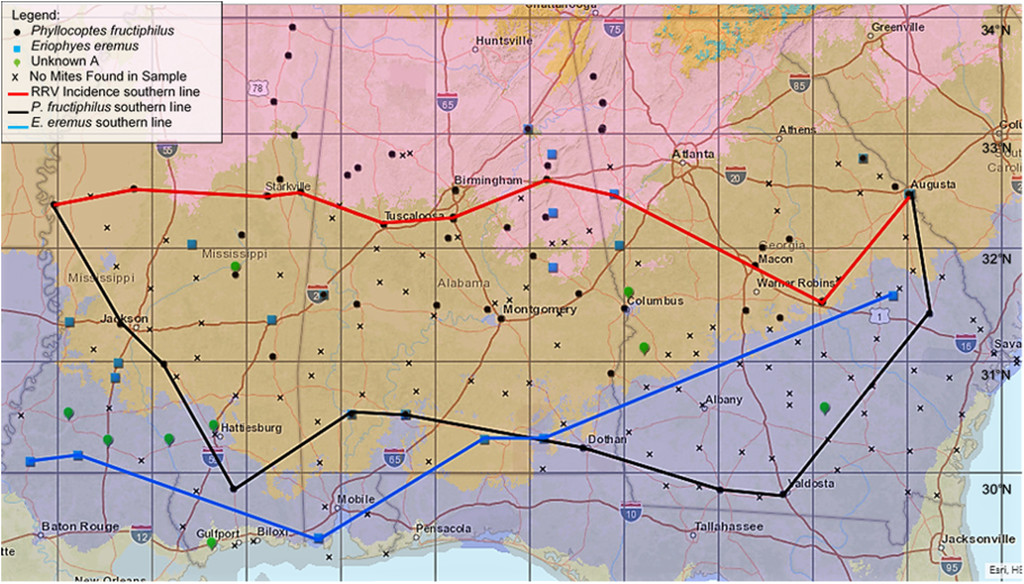
\includegraphics[width=1\linewidth]{figure/full-1288fig1} 

}

\caption[Map of the southern incidence line of \textit{{Rose rosette virus}} (RRV) and eriophyid mites, from Solo et al. 2020]{``Map of the southern incidence line of \textit{{Rose rosette virus}} (RRV) and eriophyid mites in Alabama, Georgia, and Mississippi in 2017. Plant hardiness Zone 7b is in pink, Zone 8a is brown, Zone 8b is blue, and Zone 9a is in gray. Note that there are five locations in which two mite species were found on the same rose sample.'' Citation: HortScience horts 55, 8; 10.21273/HORTSCI14653-20, CC BY-NC-ND 4.0, Unmodified from the original version.}\label{fig:solo-map-1}
\end{figure}
\begin{figure}

{\centering 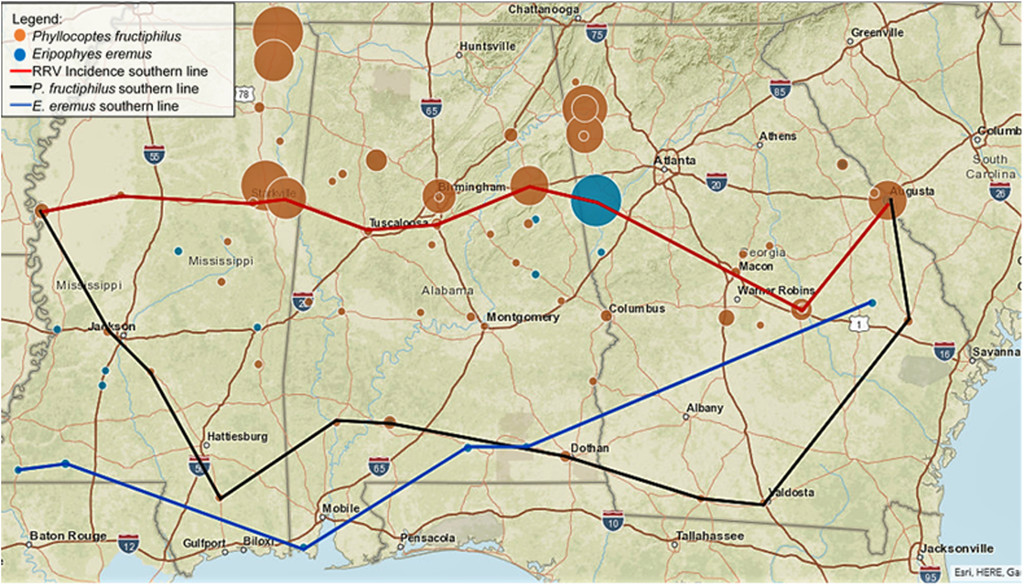
\includegraphics[width=1\linewidth]{figure/full-1288fig2} 

}

\caption[Map of the southern incidence line of Rose rosette virus (RRV), southern distribution of \textit{{Phyllocoptes fructiphilus}} and \textit{{Eriophyes eremus}}, from Solo et al. 2020]{``Map of the southern incidence line of Rose rosette virus (RRV), southern distribution of \textit{{Phyllocoptes fructiphilus}} and \textit{{Eriophyes eremus}}, and the population densities of eriophyid mites found on rose samples in Alabama, Georgia, and Mississippi in 2017. The larger the circle, the more mites found in the sample.'' Citation: HortScience horts 55, 8; 10.21273/HORTSCI14653-20, CC BY-NC-ND 4.0. Unmodified from the original version.}\label{fig:solo-map-2}
\end{figure}
\hypertarget{surveying-for-phyllocoptes-fructiphilus-rose-rosette-disease-and-predatory-mites-in-northern-florida}{%
\section{\texorpdfstring{Surveying for \emph{Phyllocoptes fructiphilus}, Rose Rosette Disease and Predatory Mites in Northern Florida}{Surveying for Phyllocoptes fructiphilus, Rose Rosette Disease and Predatory Mites in Northern Florida}}\label{surveying-for-phyllocoptes-fructiphilus-rose-rosette-disease-and-predatory-mites-in-northern-florida}}

In 2017, the entomology lab at the North Florida Research and Education Center (NFREC) in Quincy, FL, began a series of surveys of roses along the borders of northern Florida and southern Georgia. Our purpose was to estimate the distribution and populations levels of \emph{P. fructiphilus}, as well as recording any RRD incidence in northern Florida. An additional goal of the rose surveys was to detect other predatory mites present on roses: there are many species of predatory phytoseiid mites present in Florida with potential to control agricultural pests such as \emph{P. fructiphilus} (\protect\hyperlink{ref-Muma1970}{Muma and Denmark 1970}). Encountering predatory mites native to the Florida landscape may help in the development of biological control methods for \emph{P. fructiphilus}: native predatory mites sometimes have an advantage for bio-control because native mites have adapted to the environment where they will be released (\protect\hyperlink{ref-Gerson2014}{Gerson 2014}). Our results should help identify areas with greater risk for invasion, and help track the movement of \emph{P. fructiphilus} and/or RRD into Florida.

\hypertarget{materials-methods}{%
\section{Materials \& Methods}\label{materials-methods}}

A survey of roses in the landscape was conducted following a transect of northern Florida from west to east, Pensacola to Jacksonville. Cities with populations over 1,000 were visited along this route and cuttings were taken from various roses in each city \emph{(see \ref{tab:survey-table-1})}. Rose cultivar/species, sun exposure and GPS coordinates were recorded to map out sites which had predatory mites, eriophyoid mites, or possibly symptoms of RRD. Rose tissue samples were taken from the periphery of various roses in the landscape; sampling was focused on the flowering tips of roses and included a mixture of flowers, fruits, buds, and short lengths of rose cane. Samples were trimmed with bypass pruners which were routinely sanitized with 70\% ethanol between cuts. Samples were stored in 500 \si{\milli\liter} Nalgene™ Wide-Mouth Polypropylene Copolymer bottles (ThermoFisher Scientific, Waltham, MA, USA) with \textasciitilde10 \si{\milli\liter} of 95\% ethanol. The rose samples then were gently shaken to coat the rose tissues sampled with ethanol. Doing so made sure that the sampled mites were killed and acted to preserve both mites and rose tissues until samples could be processed further and checked for mites. Samples were processed using a washing method derived from Monfreda et al. (\protect\hyperlink{ref-Monfreda2007}{2007}) used to detect eriophyoid mites such as \emph{P. fructiphilius}: The sampling bottles with ethanol and rose tissues were vigorously shaken to dislodge any mites, then the ethanol in the container was poured over a stack of sieves with decreasing screen sizes: 180 \si{\micro\metre}, 53 \si{\micro\metre}, and 25 \si{\micro\metre}. The bottle and rose pieces were then further rinsed with 95\% ethanol over the sieve stack to dislodge any remaining mites. The 53 \si{\micro\metre} and 25 \si{\micro\metre} sieves were processed separately; the 53 \si{\micro\metre} sieve retained larger mites while the 25 \si{\micro\metre} sieve retained smaller mites, including \emph{P. fructiphilus}. The sieves were then backwashed from the underside of their screen with a 95\% ethanol-filled wash bottle, starting from the highest point of a sieve and working to the bottom to flush any trapped debris and mites into a 50 \si{\milli\liter} centrifuge tube for storage and future observations. The ethanol solutions of mites and plant debris were stained with a derivative of McBride's acid fuchsin stain to enhance contrast (\protect\hyperlink{ref-Backus1988}{Backus et al. 1988}). Solutions were allowed to settle until excess ethanol could be siphoned off, making it possible to then pour this concentrated plant-mite mixture into a thin, small petri dishes or a glass plate for observation under a dissecting microscope. Mites found among the plant debris were counted, then siphoned off with a glass pipette and subsequently stored in micro-centrifuge containers with 95\% ethanol as a preservative. 5-10 unstained specimens from each sample were made into prepared microscope slides: Mites were cleared and mounted using the methods of Faraji and Bakker (\protect\hyperlink{ref-Faraji2008}{2008}): mites were simultaneously cleared and stained with Faraji and Bakker's modified clearing solution and heated on a hot plate until the specimens were clear. Subsequently, these mites were moved with an eyelash tool into an iodine-modified Hoyer's slide mounting media (Hempstead Halide®, Inc., Galveston, Texas, USA), underneath a 12 \si{\milli\metre} glass coverslip. The prepared slide was then dried at 90°C before sealing the slide by painting a ring of alkyd insulating enamel (Red Glyptal® 1201, Chelsea, MA, USA) over the edges of the coverslip to seal the slide, to protect it from damage by air incursion and moisture. These slides could then be observed under a compound microscope with phase-contrast objectives to identify the mite families and species if necessary. After mite quantities and species were recorded, a representative sample of eriophyoids putatively identified as \emph{P. fructiphilus} had their identity verified with the acarologist, Dr.~Sam Bolton of the Florida Department of Agriculture and Consumer Services, Division of Plant Industry (FDACS-DPI) to ensure accuracy. Roses which appeared to show symptoms of RRD, or which had populations of \emph{P. fructiphilus} present were tested by the Plant Disease Diagnostic Clinic at the NFREC. Plant tissues were tested for RRV by Dr.~Fanny Iriarte using the currently accepted molecular methods described in Babu et al. (\protect\hyperlink{ref-Babu2016}{2016}), Babu et al. (\protect\hyperlink{ref-Babu2017a}{2017a}), and/or Babu et al. (\protect\hyperlink{ref-Babu2017b}{2017b}).

\hypertarget{results}{%
\section{Results}\label{results}}

425 samples were taken from 33 sites from an east to west transect along the border northern Florida. Eriophyoid mites were recovered in rose samples from six cities. The first samples of \emph{P. fructiphilus} were first encountered in Tallahassee during 2019; subsequent sampling efforts found in more eriophyoids in Jacksonville, Baldwin, Gainesville and Defuniak Springs in 2020, and Lake City in 2021. Other mites were collected from 68\% of the cities visited. The largest populations of \emph{P. fructiphilus} were seen in Tallahassee, with over 8,400 eriophyoid mites from 260 samples collected during 2019-2021 (\emph{see \ref{tab:survey-table-1}}). No evidence of RRD was observed in northern Florida during the surveys, even in areas where abundant \emph{P. fructiphilus} were found. Over 4,600 non-eriophyoid mites were collected from various cities during 2019-2021 \emph{\ref{tab:survey-table-1}}. Other non-eriophyoid mites collected primarily belong to the family Tetranychidae, but a small number of phytoseiidae and other predatory mites were recovered as well. These other mites currently await curation and expert identification.
\begin{figure}[p]

{\centering 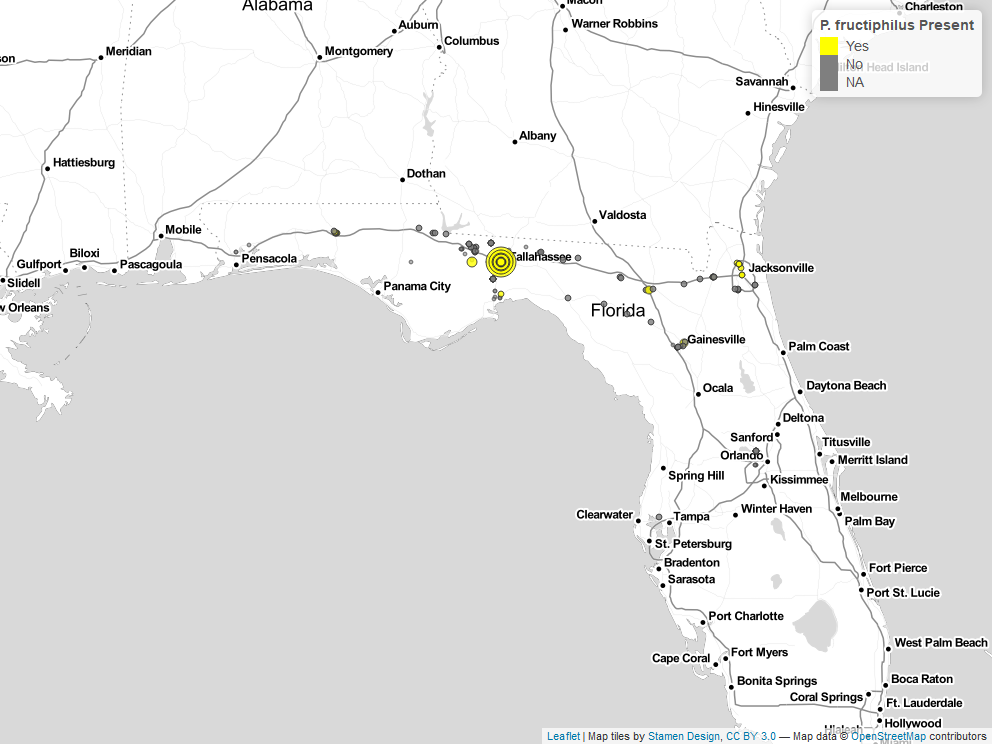
\includegraphics[width=1\linewidth]{figure/rrv_survey_map_fl_pf} 

}

\caption[\textit{P. fructiphilus} mites recovered during surveys of roses in Florida]{\textit{P. fructiphilus} mites recovered during surveys of roses in Florida, 2017-2021.}\label{fig:survey-map-1}
\end{figure}
\begin{figure}[p]

{\centering 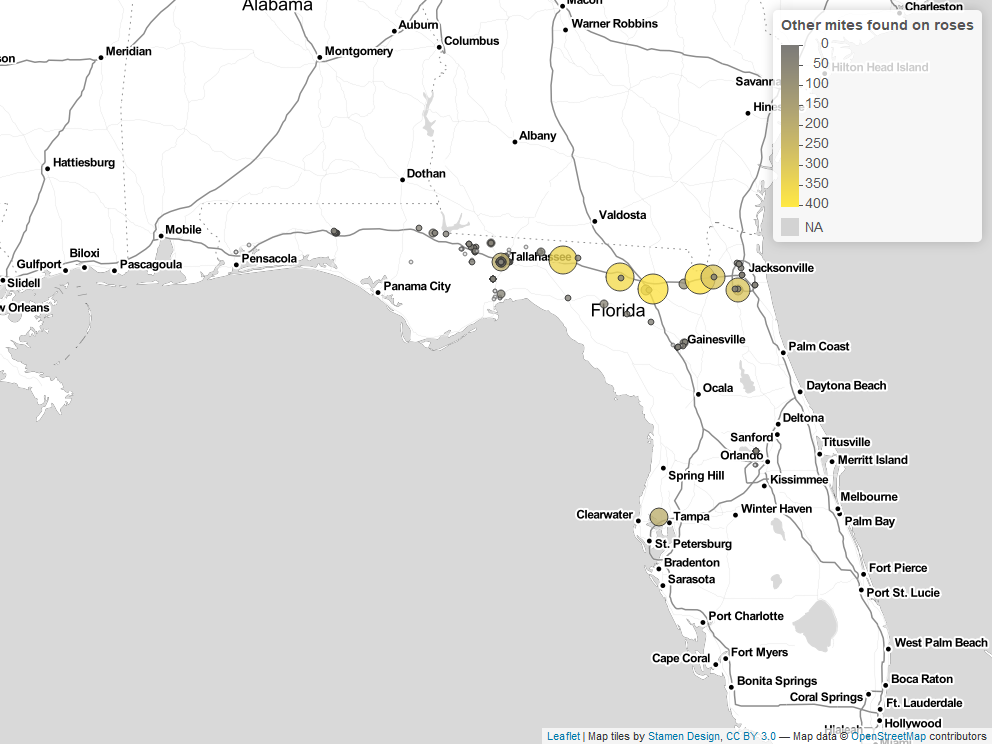
\includegraphics[width=1\linewidth]{figure/rrv_survey_map_fl_other} 

}

\caption[Other mites recovered during surveys of roses in Florida]{Other mites recovered during surveys of roses in Florida, 2017-2021.}\label{fig:survey-map-2}
\end{figure}
\begin{figure}[p]

{\centering 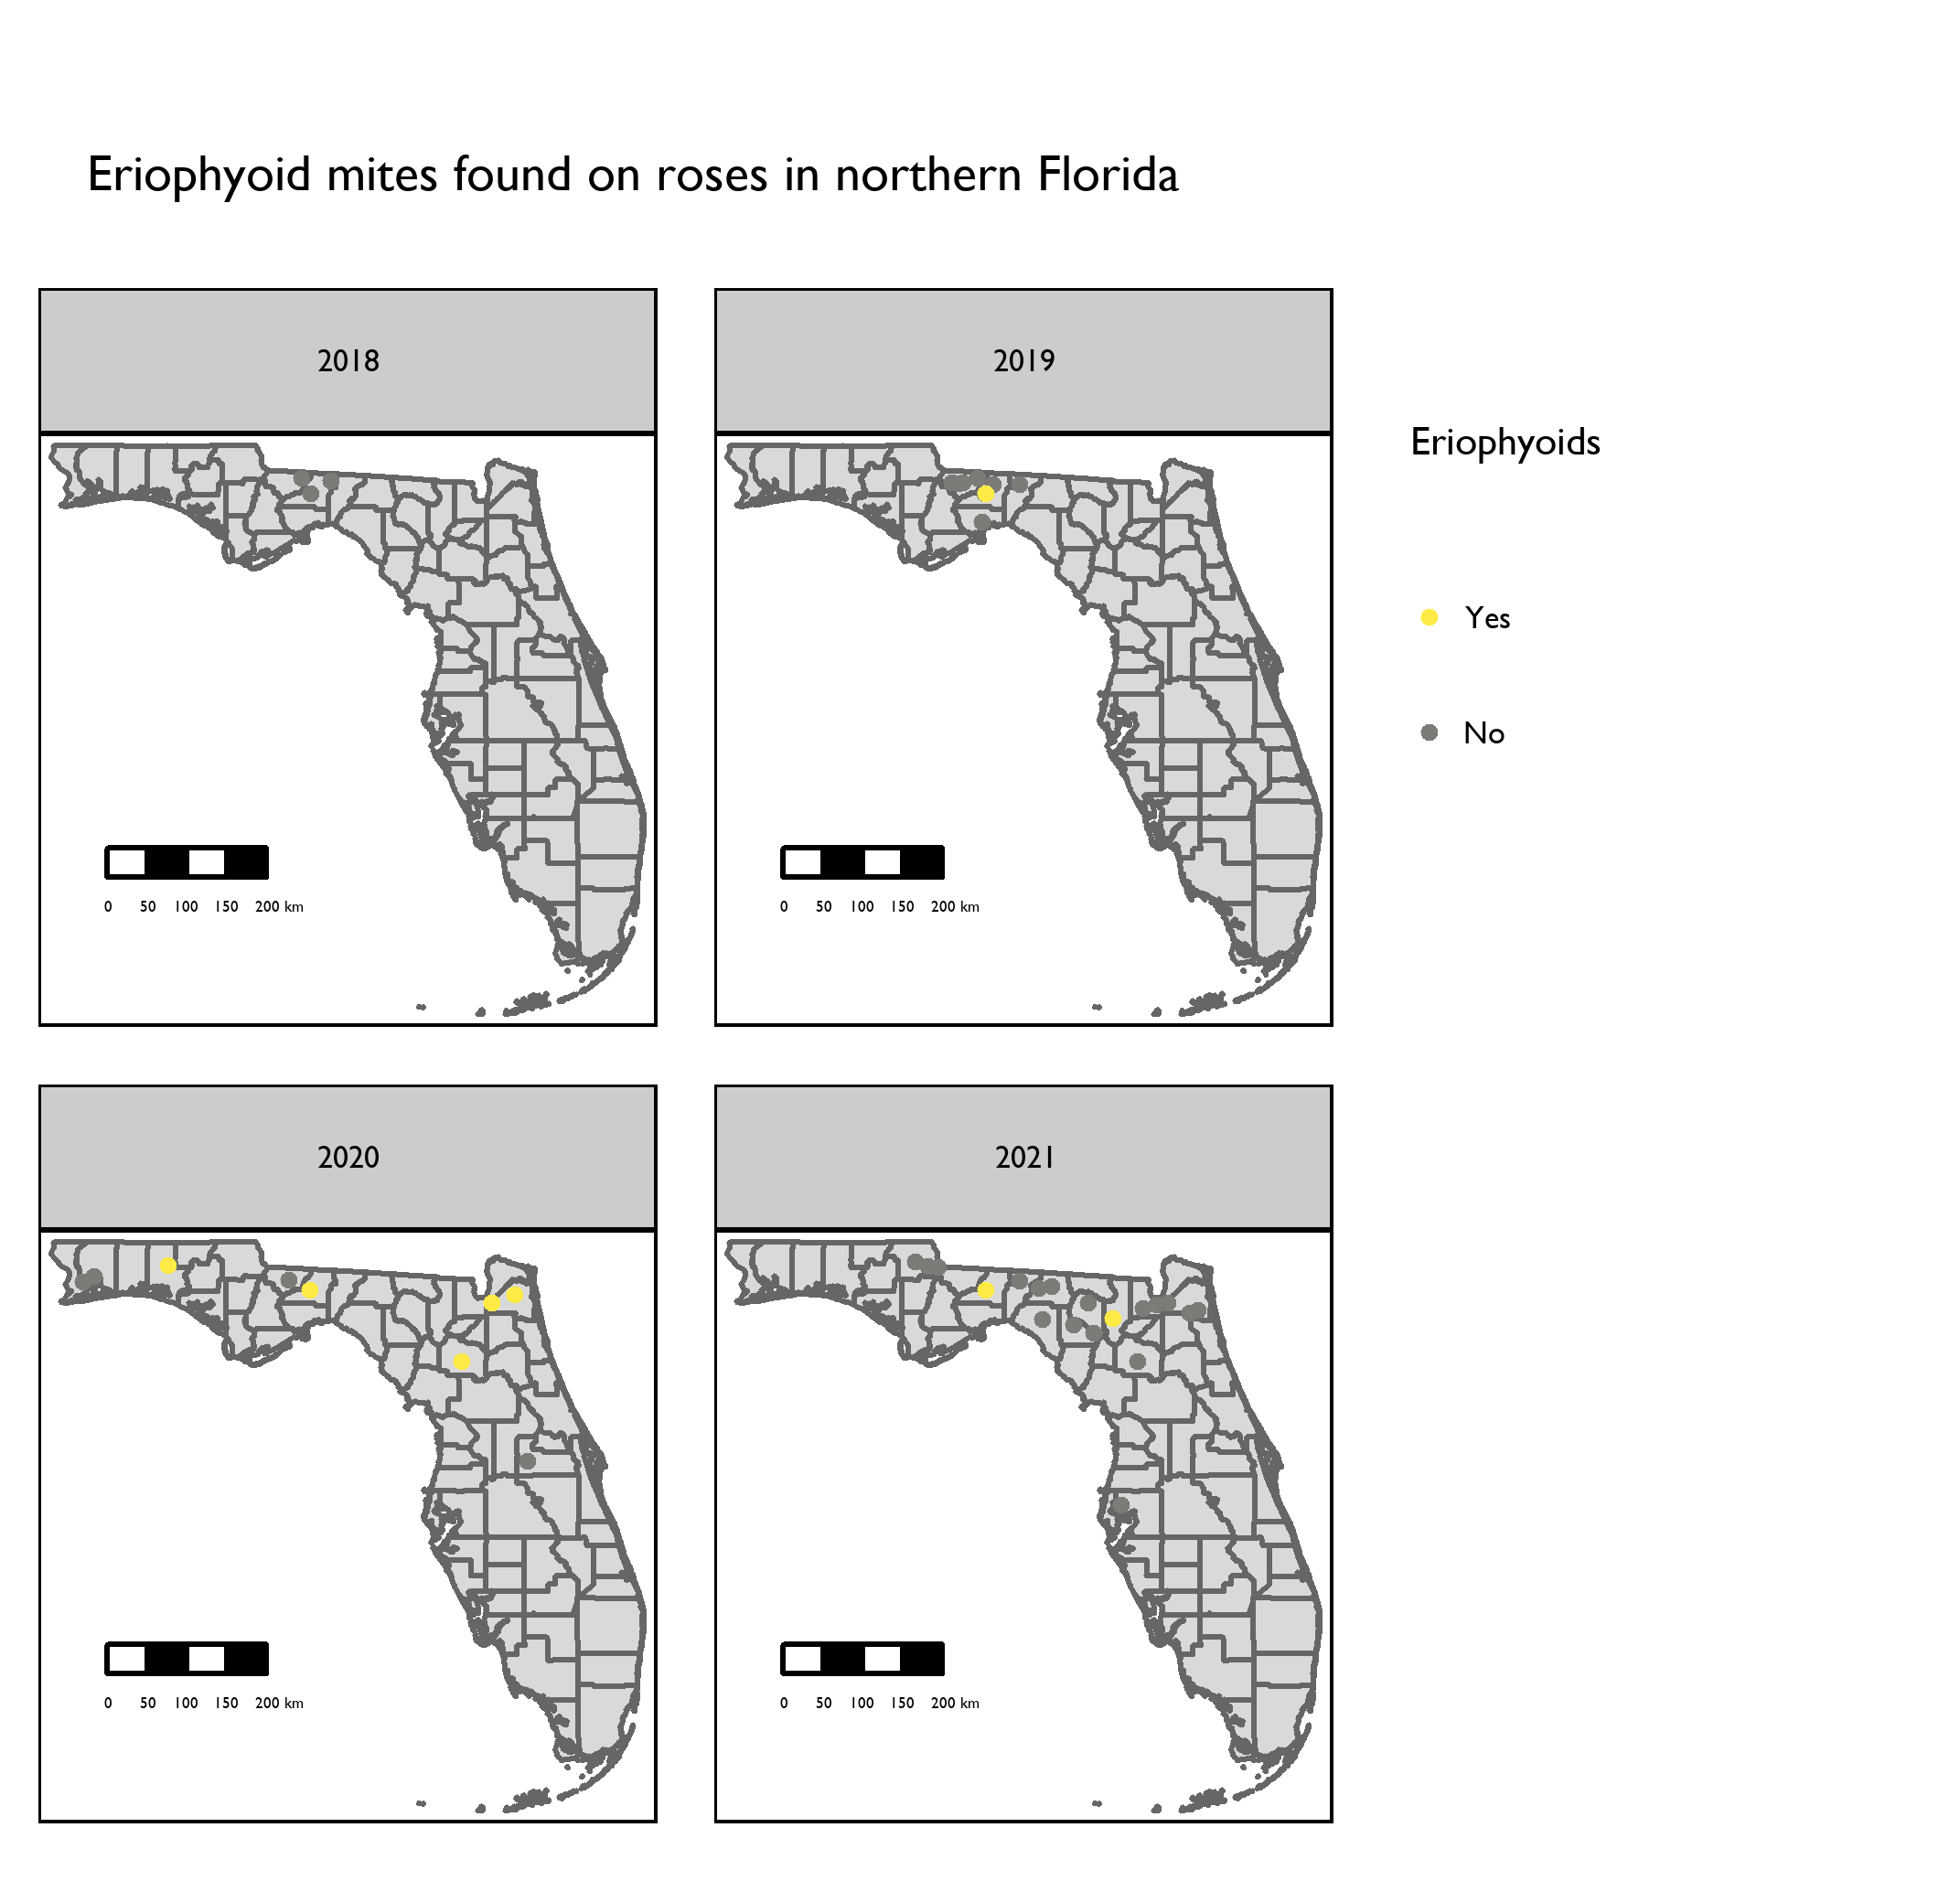
\includegraphics[width=1.25\linewidth]{figure/rrv_survey_map_years_pf} 

}

\caption[Location of populations of eriophyoid mites found on roses in northern Florida]{Location of populations of eriophyoid mites found on roses in northern Florida 2018-2021.}\label{fig:survey-map-3}
\end{figure}
\begin{figure}[p]

{\centering 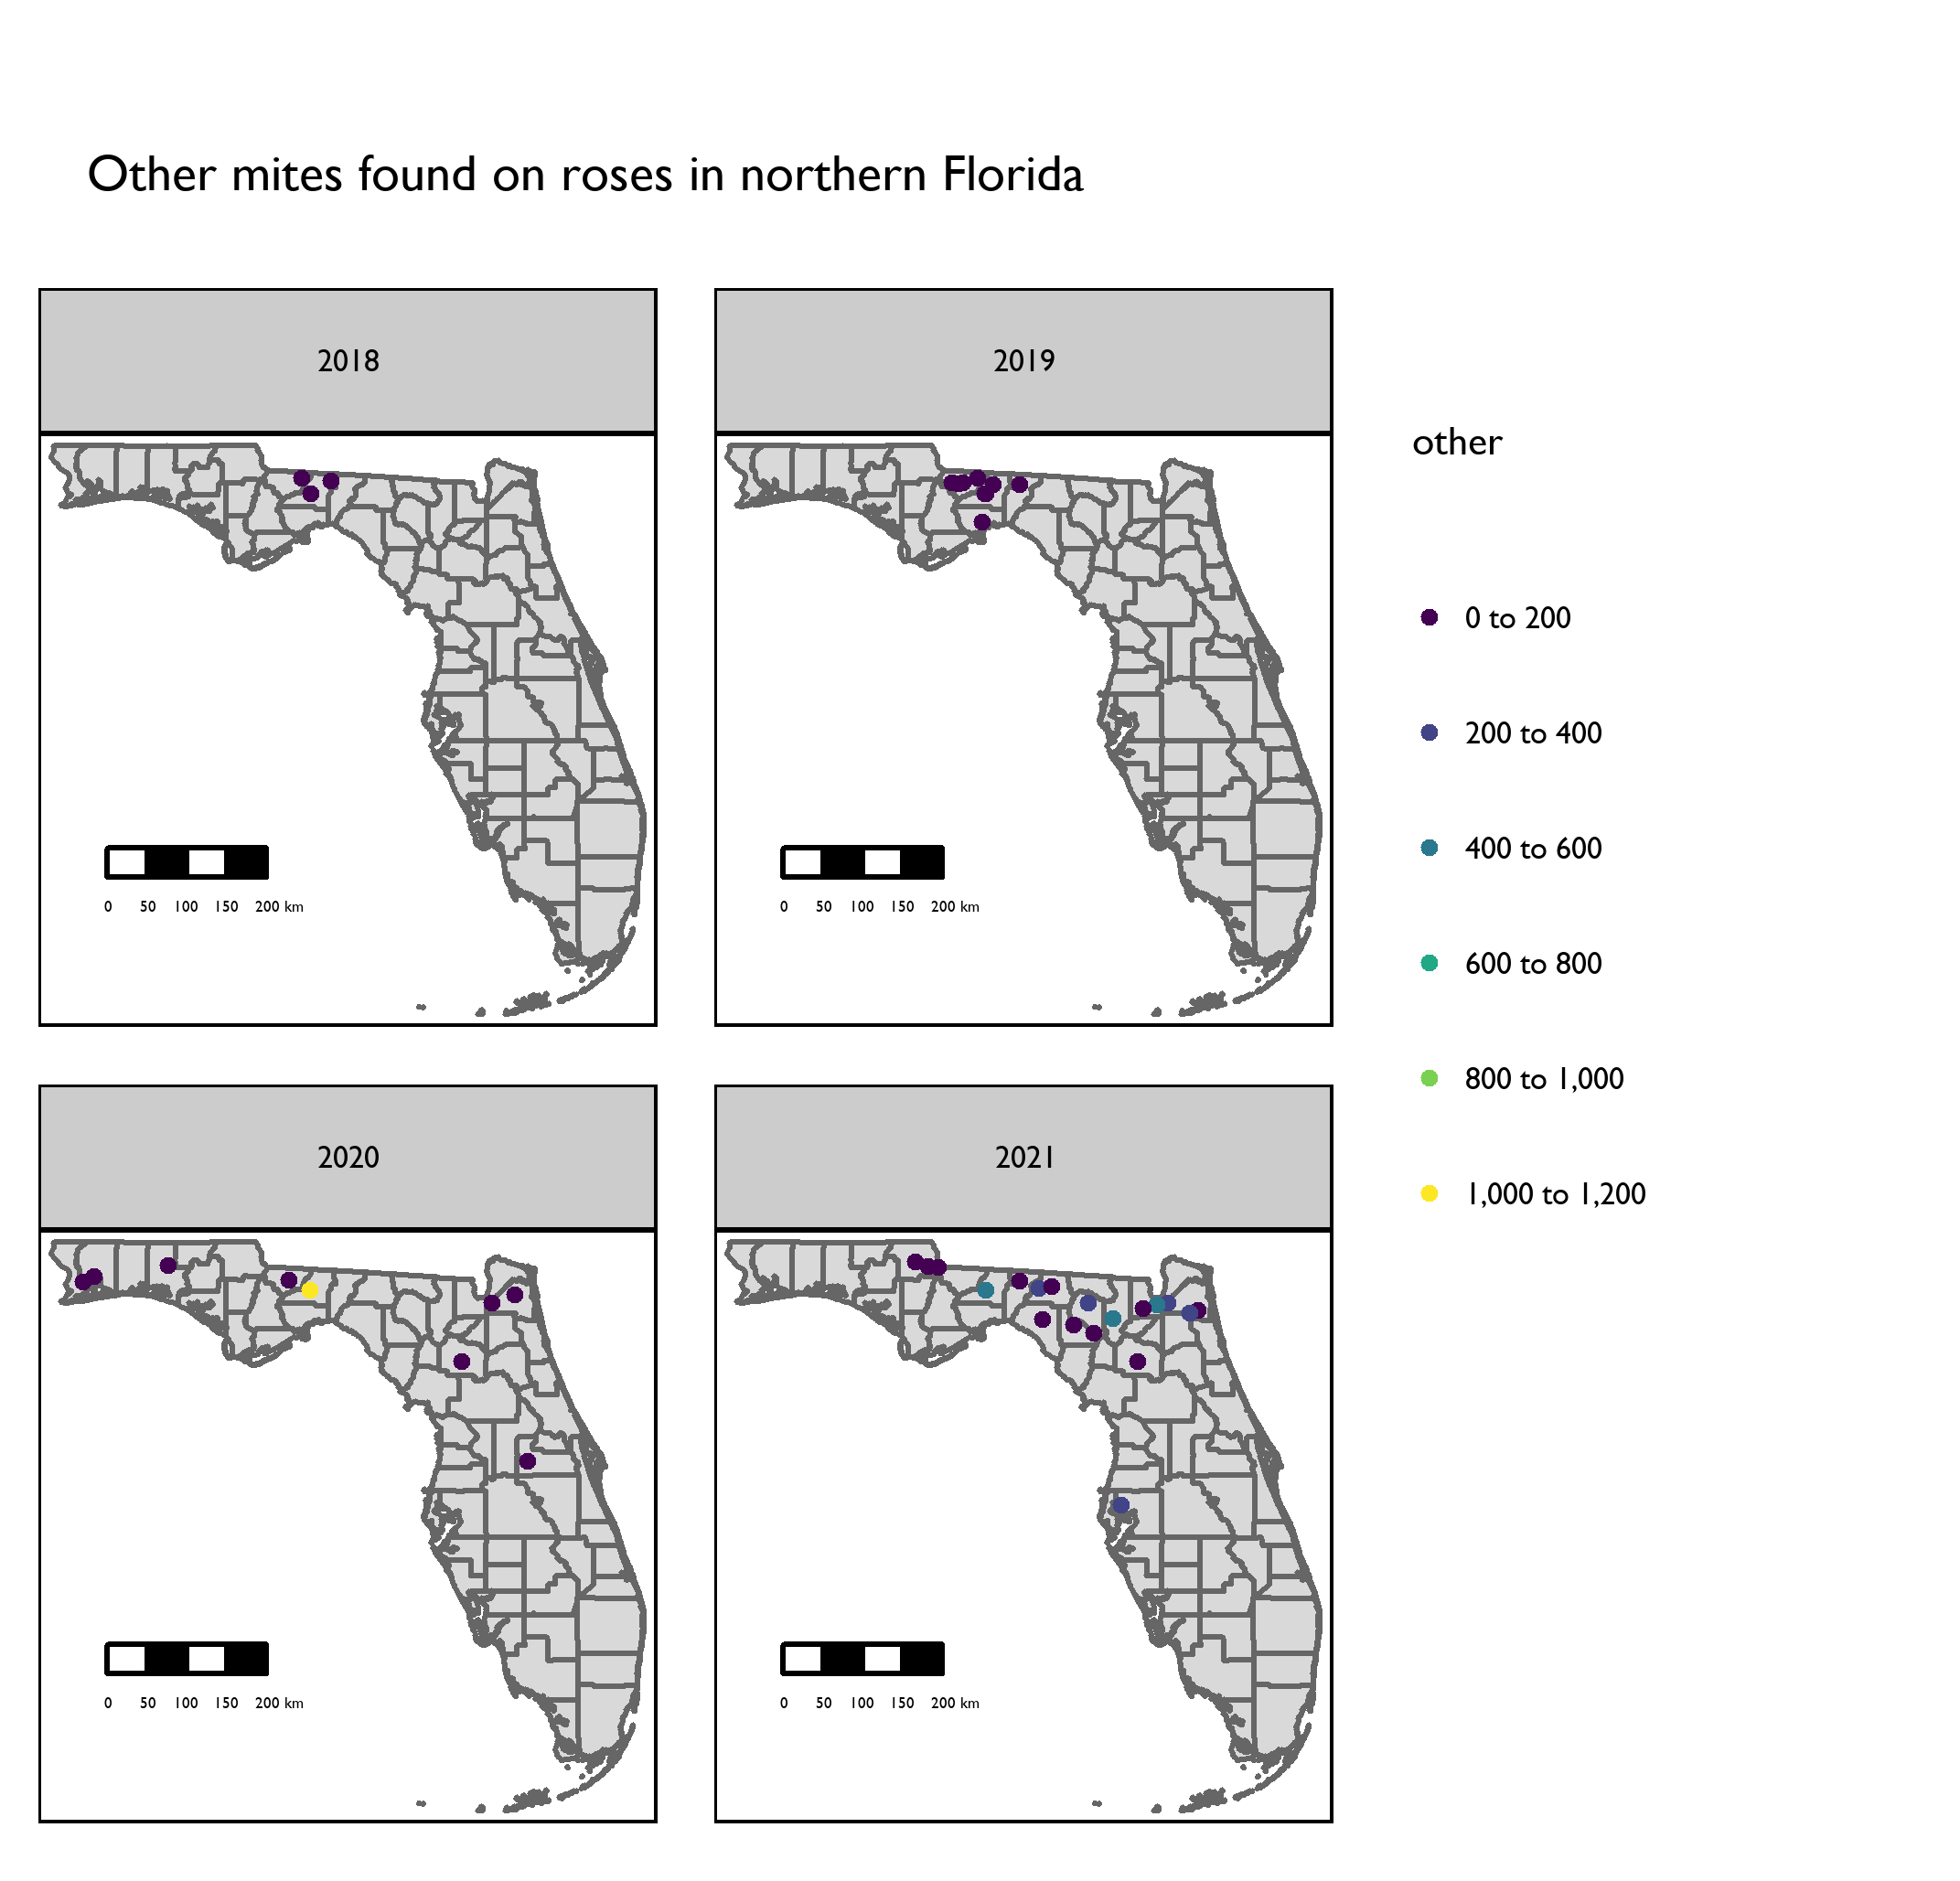
\includegraphics[width=1.25\linewidth]{figure/rrv_survey_map_years_others} 

}

\caption[Locations of other mites recovered during surveys of roses in Florida]{Locations of other mites recovered during surveys of roses in Florida, 2018-2021.}\label{fig:survey-map-4}
\end{figure}
\begin{table}[!h]

\caption{\label{tab:survey-table-1}Eriophyids and other mites recovered during surveys of roses in Florida, 2017-2021.}
\centering
\resizebox{\linewidth}{!}{
\begin{tabular}[t]{lrrrrrrrrrr}
\toprule
City & Year & Eriophyoids & Std. Error & Other Mites & Std Error & Samples per city & Eriophyoids per sample & Totals & Longitude & Latitude\\
\midrule
\cellcolor{gray!6}{Havana} & \cellcolor{gray!6}{2018} & \cellcolor{gray!6}{0} & \cellcolor{gray!6}{NA} & \cellcolor{gray!6}{0} & \cellcolor{gray!6}{NA} & \cellcolor{gray!6}{9} & \cellcolor{gray!6}{0.0} & \cellcolor{gray!6}{0} & \cellcolor{gray!6}{-84.41461} & \cellcolor{gray!6}{30.62618}\\
Miccosukee & 2018 & 0 & NA & 0 & NA & 1 & 0.0 & 0 & -84.03900 & 30.59406\\
\cellcolor{gray!6}{Tallahassee} & \cellcolor{gray!6}{2018} & \cellcolor{gray!6}{0} & \cellcolor{gray!6}{NA} & \cellcolor{gray!6}{0} & \cellcolor{gray!6}{NA} & \cellcolor{gray!6}{7} & \cellcolor{gray!6}{0.0} & \cellcolor{gray!6}{0} & \cellcolor{gray!6}{-84.29692} & \cellcolor{gray!6}{30.44227}\\
Bradfordville & 2019 & 0 & NA & 0 & NA & 2 & 0.0 & 0 & -84.21892 & 30.54678\\
\cellcolor{gray!6}{Crawfordville} & \cellcolor{gray!6}{2019} & \cellcolor{gray!6}{0} & \cellcolor{gray!6}{NA} & \cellcolor{gray!6}{0} & \cellcolor{gray!6}{NA} & \cellcolor{gray!6}{7} & \cellcolor{gray!6}{0.0} & \cellcolor{gray!6}{0} & \cellcolor{gray!6}{-84.35288} & \cellcolor{gray!6}{30.12877}\\
\addlinespace
Greensboro & 2019 & 0 & NA & 0 & NA & 5 & 0.0 & 0 & -84.74333 & 30.56824\\
\cellcolor{gray!6}{Gretna} & \cellcolor{gray!6}{2019} & \cellcolor{gray!6}{0} & \cellcolor{gray!6}{0.00} & \cellcolor{gray!6}{5} & \cellcolor{gray!6}{1.77} & \cellcolor{gray!6}{4} & \cellcolor{gray!6}{0.0} & \cellcolor{gray!6}{5} & \cellcolor{gray!6}{-84.66470} & \cellcolor{gray!6}{30.55817}\\
Havana & 2019 & 0 & 0.00 & 49 & 6.08 & 5 & 0.0 & 49 & -84.41501 & 30.62601\\
\cellcolor{gray!6}{Midway} & \cellcolor{gray!6}{2019} & \cellcolor{gray!6}{0} & \cellcolor{gray!6}{0.00} & \cellcolor{gray!6}{0} & \cellcolor{gray!6}{0.00} & \cellcolor{gray!6}{2} & \cellcolor{gray!6}{0.0} & \cellcolor{gray!6}{0} & \cellcolor{gray!6}{-84.32201} & \cellcolor{gray!6}{30.44610}\\
Monticello & 2019 & 0 & NA & 0 & NA & 7 & 0.0 & 0 & -83.87824 & 30.54454\\
\addlinespace
\cellcolor{gray!6}{Quincy} & \cellcolor{gray!6}{2019} & \cellcolor{gray!6}{0} & \cellcolor{gray!6}{0.00} & \cellcolor{gray!6}{9} & \cellcolor{gray!6}{1.13} & \cellcolor{gray!6}{7} & \cellcolor{gray!6}{0.0} & \cellcolor{gray!6}{9} & \cellcolor{gray!6}{-84.60175} & \cellcolor{gray!6}{30.56986}\\
Tallahassee & 2019 & 4704 & 9.86 & 47 & 0.29 & 79 & 59.5 & 4751 & -84.30902 & 30.44618\\
\cellcolor{gray!6}{Baldwin} & \cellcolor{gray!6}{2020} & \cellcolor{gray!6}{27} & \cellcolor{gray!6}{1.31} & \cellcolor{gray!6}{15} & \cellcolor{gray!6}{1.55} & \cellcolor{gray!6}{4} & \cellcolor{gray!6}{6.8} & \cellcolor{gray!6}{42} & \cellcolor{gray!6}{-81.97352} & \cellcolor{gray!6}{30.30268}\\
Defuniak Springs & 2020 & 20 & 2.06 & 29 & 0.70 & 6 & 3.3 & 49 & -86.12718 & 30.72614\\
\cellcolor{gray!6}{Ferry Pass} & \cellcolor{gray!6}{2020} & \cellcolor{gray!6}{0} & \cellcolor{gray!6}{NA} & \cellcolor{gray!6}{0} & \cellcolor{gray!6}{NA} & \cellcolor{gray!6}{2} & \cellcolor{gray!6}{0.0} & \cellcolor{gray!6}{0} & \cellcolor{gray!6}{-87.21893} & \cellcolor{gray!6}{30.54415}\\
\addlinespace
Gainesville & 2020 & 25 & 3.23 & 55 & 4.60 & 20 & 1.2 & 80 & -82.36118 & 29.64316\\
\cellcolor{gray!6}{Jacksonville} & \cellcolor{gray!6}{2020} & \cellcolor{gray!6}{66} & \cellcolor{gray!6}{1.13} & \cellcolor{gray!6}{41} & \cellcolor{gray!6}{1.67} & \cellcolor{gray!6}{8} & \cellcolor{gray!6}{8.2} & \cellcolor{gray!6}{107} & \cellcolor{gray!6}{-81.68811} & \cellcolor{gray!6}{30.39848}\\
Milton & 2020 & 0 & NA & 0 & NA & 1 & 0.0 & 0 & -87.07610 & 30.60700\\
\cellcolor{gray!6}{Orlando} & \cellcolor{gray!6}{2020} & \cellcolor{gray!6}{0} & \cellcolor{gray!6}{NA} & \cellcolor{gray!6}{0} & \cellcolor{gray!6}{NA} & \cellcolor{gray!6}{4} & \cellcolor{gray!6}{0.0} & \cellcolor{gray!6}{0} & \cellcolor{gray!6}{-81.51605} & \cellcolor{gray!6}{28.50670}\\
Quincy & 2020 & 0 & NA & 0 & NA & 1 & 0.0 & 0 & -84.57331 & 30.55638\\
\addlinespace
\cellcolor{gray!6}{Tallahassee} & \cellcolor{gray!6}{2020} & \cellcolor{gray!6}{3364} & \cellcolor{gray!6}{4.82} & \cellcolor{gray!6}{1150} & \cellcolor{gray!6}{0.79} & \cellcolor{gray!6}{157} & \cellcolor{gray!6}{21.4} & \cellcolor{gray!6}{4514} & \cellcolor{gray!6}{-84.30878} & \cellcolor{gray!6}{30.44297}\\
Baldwin & 2021 & 0 & 0.00 & 309 & 145.50 & 2 & 0.0 & 309 & -81.97613 & 30.30260\\
\cellcolor{gray!6}{Branford} & \cellcolor{gray!6}{2021} & \cellcolor{gray!6}{0} & \cellcolor{gray!6}{NA} & \cellcolor{gray!6}{12} & \cellcolor{gray!6}{NA} & \cellcolor{gray!6}{1} & \cellcolor{gray!6}{0.0} & \cellcolor{gray!6}{12} & \cellcolor{gray!6}{-82.92316} & \cellcolor{gray!6}{29.95685}\\
Gainesville & 2021 & 0 & 0.00 & 6 & 1.00 & 2 & 0.0 & 6 & -82.36566 & 29.63691\\
\cellcolor{gray!6}{Grand Ridge} & \cellcolor{gray!6}{2021} & \cellcolor{gray!6}{0} & \cellcolor{gray!6}{0.00} & \cellcolor{gray!6}{30} & \cellcolor{gray!6}{11.00} & \cellcolor{gray!6}{2} & \cellcolor{gray!6}{0.0} & \cellcolor{gray!6}{30} & \cellcolor{gray!6}{-85.04182} & \cellcolor{gray!6}{30.71944}\\
\addlinespace
Greenville & 2021 & 0 & NA & 356 & NA & 1 & 0.0 & 356 & -83.63092 & 30.46842\\
\cellcolor{gray!6}{Greenwood} & \cellcolor{gray!6}{2021} & \cellcolor{gray!6}{0} & \cellcolor{gray!6}{NA} & \cellcolor{gray!6}{200} & \cellcolor{gray!6}{NA} & \cellcolor{gray!6}{1} & \cellcolor{gray!6}{0.0} & \cellcolor{gray!6}{200} & \cellcolor{gray!6}{-82.57149} & \cellcolor{gray!6}{28.00751}\\
Jacksonville & 2021 & 0 & 0.00 & 12 & 2.65 & 3 & 0.0 & 12 & -81.59286 & 30.21992\\
\cellcolor{gray!6}{Lake City} & \cellcolor{gray!6}{2021} & \cellcolor{gray!6}{49} & \cellcolor{gray!6}{9.80} & \cellcolor{gray!6}{472} & \cellcolor{gray!6}{77.72} & \cellcolor{gray!6}{5} & \cellcolor{gray!6}{9.8} & \cellcolor{gray!6}{521} & \cellcolor{gray!6}{-82.67590} & \cellcolor{gray!6}{30.12273}\\
Live Oak & 2021 & 0 & 0.00 & 376 & 182.00 & 2 & 0.0 & 376 & -82.99862 & 30.30259\\
\addlinespace
\cellcolor{gray!6}{Macclenny} & \cellcolor{gray!6}{2021} & \cellcolor{gray!6}{0} & \cellcolor{gray!6}{NA} & \cellcolor{gray!6}{400} & \cellcolor{gray!6}{NA} & \cellcolor{gray!6}{1} & \cellcolor{gray!6}{0.0} & \cellcolor{gray!6}{400} & \cellcolor{gray!6}{-82.11797} & \cellcolor{gray!6}{30.28349}\\
Madison & 2021 & 0 & NA & 14 & NA & 1 & 0.0 & 14 & -83.46405 & 30.48829\\
\cellcolor{gray!6}{Marianna} & \cellcolor{gray!6}{2021} & \cellcolor{gray!6}{0} & \cellcolor{gray!6}{NA} & \cellcolor{gray!6}{11} & \cellcolor{gray!6}{NA} & \cellcolor{gray!6}{1} & \cellcolor{gray!6}{0.0} & \cellcolor{gray!6}{11} & \cellcolor{gray!6}{-85.20554} & \cellcolor{gray!6}{30.76829}\\
Mayo & 2021 & 0 & NA & 32 & NA & 1 & 0.0 & 32 & -83.18075 & 30.05482\\
\cellcolor{gray!6}{Monticello} & \cellcolor{gray!6}{2021} & \cellcolor{gray!6}{0} & \cellcolor{gray!6}{NA} & \cellcolor{gray!6}{20} & \cellcolor{gray!6}{NA} & \cellcolor{gray!6}{1} & \cellcolor{gray!6}{0.0} & \cellcolor{gray!6}{20} & \cellcolor{gray!6}{-83.87114} & \cellcolor{gray!6}{30.54514}\\
\addlinespace
Orange Park & 2021 & 0 & 0.00 & 363 & 90.28 & 3 & 0.0 & 363 & -81.70203 & 30.18646\\
\cellcolor{gray!6}{Perry} & \cellcolor{gray!6}{2021} & \cellcolor{gray!6}{0} & \cellcolor{gray!6}{NA} & \cellcolor{gray!6}{3} & \cellcolor{gray!6}{NA} & \cellcolor{gray!6}{1} & \cellcolor{gray!6}{0.0} & \cellcolor{gray!6}{3} & \cellcolor{gray!6}{-83.57833} & \cellcolor{gray!6}{30.11150}\\
Sanderson & 2021 & 0 & NA & 78 & NA & 1 & 0.0 & 78 & -82.29722 & 30.24098\\
\cellcolor{gray!6}{Sneads} & \cellcolor{gray!6}{2021} & \cellcolor{gray!6}{0} & \cellcolor{gray!6}{NA} & \cellcolor{gray!6}{1} & \cellcolor{gray!6}{NA} & \cellcolor{gray!6}{1} & \cellcolor{gray!6}{0.0} & \cellcolor{gray!6}{1} & \cellcolor{gray!6}{-84.91279} & \cellcolor{gray!6}{30.71067}\\
Tallahassee & 2021 & 424 & 2.78 & 579 & 8.68 & 24 & 17.7 & 1003 & -84.30731 & 30.44491\\
\addlinespace
\cellcolor{gray!6}{Grand Totals} & \cellcolor{gray!6}{2021} & \cellcolor{gray!6}{8679} & \cellcolor{gray!6}{NA} & \cellcolor{gray!6}{4674} & \cellcolor{gray!6}{NA} & \cellcolor{gray!6}{425} & \cellcolor{gray!6}{127.9} & \cellcolor{gray!6}{13353} & \cellcolor{gray!6}{-83.71379} & \cellcolor{gray!6}{30.25158}\\
\bottomrule
\end{tabular}}
\end{table}
\hypertarget{discussion}{%
\section{Discussion}\label{discussion}}

The presence of \emph{P. fructiphilus} in northern Florida over multiple years and seasons provides evidence against a putative southern limit for the species (\protect\hyperlink{ref-Solo2020}{Solo et al. 2020}). Unfortunately, our survey efforts were severely hampered by the COVID-19 pandemic, which limited opportunities to travel and collect mites. We expect that further investigations of roses in other Florida cities will reveal more \emph{P. fructiphilus}-infested sites. The arrival of a competent vector is not a guarantee that its associated disease will follow suit, but it does provide a necessary component of the disease triangle: if the environmental conditions are suitable, and the rose host is sufficiently abundant, there is potential for disease to occur (\protect\hyperlink{ref-Francl2001}{Francl 2001}). We did not see any signs of RRD in roses in northern Florida, but it is important to note that the delayed onset and difficulty of identifying symptoms makes it likely to miss detection until late stages of the disease. It is not known how \emph{P. fructiphilus} have arrived in northern Florida, or how long they have been here, and unfortunately our observations are not sufficient to describe a mechanism of invasion. Eriophyoid mites may be windblown, transported with infected plants, move on contaminated equipment or clothes, or rarely, are moved through phoresy (\protect\hyperlink{ref-Sabelis1996}{Sabelis and Bruin 1996}). Previous Florida mite surveys were conducted in 2017 and 2018, along a north-south transect from Florida into Georgia, but \emph{P. fructiphilus} were only detected in recent years. The 2017-2018 Florida surveys were focused on Cherokee roses \emph{Rosa laevigata}, roses which are easiest to find during the spring and early summer, due to their ephemeral blooming cycle. Our recent surveys did not cover the same locations and focused on all species roses present in public or private plantings. In addition, we were unable to sample from Cherokee roses in Florida, due to COVID-19 lockdowns travel restrictions during the blooming season of \emph{R. laevigata}. The sites with the largest populations of \emph{P fructiphilus} in Florida are various plantings around of a college campus, with many landscaping projects, allowing for many potential introductions of \emph{P. fructiphilus} on newly purchased plants. On the other hand, the current invasions of \emph{P. fructiphilus} may have been introduced through their natural means of dispersal over time. The short distances between mite infested roses in Georgia, Alabama and Florida suggest the possibility of multiple routes of introduction, but the mechanisms of dispersal require further investigation for \emph{P. fructiphilus}. In addition, the movements of plant pathogens such as RRD is thought to be partially driven by socioeconomic factors and the movement of plants by people (\protect\hyperlink{ref-Nelson2015}{Nelson and Bone 2015}, \protect\hyperlink{ref-Katsiani2020}{Katsiani et al. 2020}). Inspections and quarantines of mite-infested roses by wholesalers and larger growers is predicted to slow the spread of plant pathogen epidemics (\protect\hyperlink{ref-Nelson2015}{Nelson and Bone 2015}). A large number of other non-eriophyoid mites have been collected. Our findings were similar to the results of other surveys (\protect\hyperlink{ref-Jesse2006}{Jesse et al. 2006}, \protect\hyperlink{ref-Otero-Colina2018}{Otero-Colina et al. 2018}, \protect\hyperlink{ref-Solo2020}{Solo et al. 2020}): we primarily encountered plant-feeding mites, including mites from the families tetranychidae, tenuipalpidae, eriophyoidae, and some predators, including chelytidae and phytoseiidae. We did encounter some tydeidae, but we are not certain of their feeding guild, as many tydeidae are fungivores rather than herbivores. Further examination of collected mites is expected to reveal a variety of species and overlooked individuals. Accurate identification will necessarily require collaboration with individuals better trained in mite taxonomy to avoid misidentifications (\protect\hyperlink{ref-Demard2021}{Demard et al. 2021}). In conclusion, the presence of \emph{P. fructiphilus} in Florida necessitates the development of mite control practices to prevent mite populations from surging, and to hopefully prevent the spread of RRD.

\hypertarget{changes-in-headspace-volatiles-for-roses-infected-with-rose-rosette-disease}{%
\chapter{CHANGES IN HEADSPACE VOLATILES FOR ROSES INFECTED WITH ROSE ROSETTE DISEASE}\label{changes-in-headspace-volatiles-for-roses-infected-with-rose-rosette-disease}}

\hypertarget{introduction-1}{%
\section{Introduction}\label{introduction-1}}

\hypertarget{plant-defenses-and-volatiles-why-are-amblyseius-swirskii-attracted-infected-roses}{%
\subsection{\texorpdfstring{Plant defenses and volatiles: why are \emph{Amblyseius swirskii} attracted infected roses?}{Plant defenses and volatiles: why are Amblyseius swirskii attracted infected roses?}}\label{plant-defenses-and-volatiles-why-are-amblyseius-swirskii-attracted-infected-roses}}

Rose Rosette Virus (RRV) genus \emph{Emaraviridae} is the the casual agent of Rose Rosette Disease (RRD), the most severe disease of roses (\protect\hyperlink{ref-Laney2011}{Laney et al. 2011}). RRD is thought to have invaded the southeastern United States by the movement of its vector, the eriophyid mite, \emph{Phyllocoptes fructiphilus} Kiefer (Trombidiformes: Eriophyidae), on multiflora rose (\emph{Rosa multiflora} (Thunb)), as these organisms expanded their range from the US northwest, south and east towards the coast (\protect\hyperlink{ref-Amrine2002}{Amrine Jr 2002}, \protect\hyperlink{ref-Otero-Colina2018}{Otero-Colina et al. 2018}, \protect\hyperlink{ref-Solo2020}{Solo et al. 2020}). RRD is currently present throughout the US, and has been recently detected in Florida (\protect\hyperlink{ref-Fife2020}{Fife et al. 2020}). Infection with RRD creates witches' brooms, rosetting, deforms flowers, increases prickle density, elongates shoots, reddens of plant tissues, causes die-back and ultimately plant death. Few management options are available to manage \emph{P. fructiphilus}: Current mite control is achieved by removing infected roses and frequent pesticide applications (\protect\hyperlink{ref-Hong2012}{Hong et al. 2012}, \protect\hyperlink{ref-Olson2017}{Olson et al. 2017}, \protect\hyperlink{ref-UGA2018}{{``Control - rose rosette''} 2018}). Nursery managers are interested in additional management options to combat \emph{P. fructiphilus} and RRD. Induced plant defenses offer an important potential role in the prevention of disease and control of insect pests (\protect\hyperlink{ref-Walling2000}{Walling 2000}, \protect\hyperlink{ref-Farmer2016}{Farmer 2016}). When plants detect elicitors from a pathogen or an herbivore (\protect\hyperlink{ref-Mithoefer2008}{Mithöfer and Boland 2008}, \protect\hyperlink{ref-Boller2009}{Boller and Felix 2009}), they respond by upregulating intercellular Salicylic Acid (SA), initiating a process known as systemic acquired resistance (SAR) (\protect\hyperlink{ref-Gaffney1993}{Gaffney et al. 1993}, \protect\hyperlink{ref-Goodman1994}{Goodman and Novacky 1994}, \protect\hyperlink{ref-Park2007}{Park et al. 2007}, \protect\hyperlink{ref-Vlot2009}{Vlot et al. 2009}). Induction of SAR helps to provide protection from herbivory as well as pathogen damage (\protect\hyperlink{ref-Cole1999}{Cole 1999}, \protect\hyperlink{ref-Anfoka2000}{Anfoka 2000}, \protect\hyperlink{ref-Babu2021}{Babu et al. 2021}, \protect\hyperlink{ref-Doungous2021}{Doungous et al. 2021}). Inducing SAR can have various positive effects on disease prevention: SAR induction is often used to combat fungal diseases (\protect\hyperlink{ref-Goy1992}{Goy et al. 1992}, \protect\hyperlink{ref-Xue1998}{Xue et al. 1998}, \protect\hyperlink{ref-Narusaka1999}{Narusaka et al. 1999}, \protect\hyperlink{ref-Suo2001}{Suo and Leung 2001}), and some studies have found that SAR induction and the hypersensitive response can disrupt the establishment of eriophyoid mites (\protect\hyperlink{ref-Bronner1991}{Bronner et al. 1991a}, \protect\hyperlink{ref-Bronner1991a}{1991b}, \protect\hyperlink{ref-Westphal1991}{Westphal et al. 1991}). Infested plants produce \textbeta-1,3-glucanase and chitinases, which were hypothesized to contribute to plant defenses against eriophyoid mites (\protect\hyperlink{ref-Bronner1991a}{Bronner et al. 1991b}, \protect\hyperlink{ref-Ward1991a}{Ward et al. 1991}). Similar increases in \textbeta-1,3-glucanase and chitinase activity was seen in roses treated with acibenzolar-S-methyl (ASM), a benzothiadiazole known used to induce SAR (\protect\hyperlink{ref-Cole1999}{Cole 1999}, \protect\hyperlink{ref-Darolt2020}{Darolt et al. 2020}, \protect\hyperlink{ref-Doungous2021}{Doungous et al. 2021}). Applications of ASM have also been reported to help restrict the growth of fungal pathogens in roses (\protect\hyperlink{ref-Suo2001}{Suo and Leung 2001}), and purportedly control populations of whiteflies (\protect\hyperlink{ref-Correa2005}{Correa et al. 2005}, \protect\hyperlink{ref-Doungous2021}{Doungous et al. 2021}) as well as aphids (\protect\hyperlink{ref-Costa2006}{Costa and Moraes 2006}). We hypothesize that SAR-induction in roses may be able to reduce populations of \emph{P. fructiphilus} as well. Unfortunately, inducing SAR can have negative effects on herbivores as well as predators (\protect\hyperlink{ref-Kant2015}{Kant et al. 2015}, \protect\hyperlink{ref-Ataide2016}{Ataide et al. 2016}, \protect\hyperlink{ref-Pappas2017}{Pappas et al. 2017}), which necessitates careful study of all organisms involved in the system to create a successful pest management program. A handful of studies tested \emph{Amblyseius swirskii} Athias-Henriot (Mesostigmata: Phytoseiidae), for their suitability to control pests on ornamental roses (\protect\hyperlink{ref-Chow2010}{Chow et al. 2010}, \protect\hyperlink{ref-Hoogerbrugge2011}{Hoogerbrugge et al. 2011}, \protect\hyperlink{ref-Hoogerbrugge2014}{Hoogerbrugge et al. 2014}, \protect\hyperlink{ref-Alipour2016}{Alipour et al. 2016}, \protect\hyperlink{ref-Alipour2019}{2019}). \emph{A. swirskii} is one of the most popular species of commercially-available phytoseiid mites (\protect\hyperlink{ref-Calvo2014}{Calvo et al. 2014}), but has been seldom used in ornamental crops (\protect\hyperlink{ref-Buitenhuis2015}{Buitenhuis et al. 2015}). \emph{A. swirskii} are considered to be a generalist species which feed on a variety of different arthropod pests, including thrips, whiteflies, and occasionally other mites (\protect\hyperlink{ref-McMurtry1997}{McMurtry and Croft 1997}, \protect\hyperlink{ref-Bolckmans2005}{Bolckmans et al. 2005}, \protect\hyperlink{ref-Hoogerbrugge2014}{Hoogerbrugge et al. 2014}), and there is growing interest in using them on ornamental crops to control pests commonly encountered in roses (\protect\hyperlink{ref-Chow2010}{Chow et al. 2010}, \protect\hyperlink{ref-Buitenhuis2015}{Buitenhuis et al. 2015}, \protect\hyperlink{ref-Schoeller2020}{Schoeller et al. 2020}). Phytoseiid like \emph{A. swirskii} have no eyes, instead relying on plant VOCs to guide them to their prey (\protect\hyperlink{ref-Gnanvossou2003}{Gnanvossou et al. 2003}, \protect\hyperlink{ref-Boer2004a}{Boer and Dicke 2004a}, \protect\hyperlink{ref-Nomikou2005}{Nomikou et al. 2005}). Many plant VOCs are released when a plant is attacked by herbivores or pathogens (\protect\hyperlink{ref-Shulaev1997}{Shulaev et al. 1997}, \protect\hyperlink{ref-Sabelis1999}{Sabelis et al. 1999}, \protect\hyperlink{ref-Ozawa2000}{Ozawa et al. 2000}, \protect\hyperlink{ref-Halitschke2007}{Halitschke et al. 2007}), the composition of which varies, depending on the plant species and type of damage/infection (\protect\hyperlink{ref-Sabelis1999}{Sabelis et al. 1999}, \protect\hyperlink{ref-Boom2004}{Boom et al. 2004}, \protect\hyperlink{ref-Maeda2006}{Maeda and Liu 2006}, \protect\hyperlink{ref-Qualley2008}{Qualley and Dudareva 2008}). Volatiles also deter herbivores or attract predators (\protect\hyperlink{ref-Pichersky2002}{Pichersky and Gershenzon 2002}), so it important to understand which chemicals may manipulate the behaviors of released biological agents in the same system. Studies by Farber et al. (\protect\hyperlink{ref-Farber2019}{2019}) found differences between healthy and RRV-infected roses using Raman spectroscopy at a spectral band of 1720 \si{\centi\meter}\^{}\{−1\}\$, a spectral region associated with carbonyl stretching vibrations. This indicates the presence of carbonyl compounds, a group functional group commonly seen in many organic compounds, including esters, aldehydes, carboxylic acids, and ketones. Farber et al. (\protect\hyperlink{ref-Farber2019}{2019}) suggested that bands may be evidence for the presence of the carboxylic compounds Jasmonic Acid and Salicyclic Acid, due to the association of these plant hormones with plant defenses against pathogens (\protect\hyperlink{ref-Verma2016}{Verma et al. 2016}). When SAR is induced, SA becomes methylated and converts to Methyl Salicylate (MeSA), a volatile signal which helps to propagate resistance throughout the plant (\protect\hyperlink{ref-Shulaev1997}{Shulaev et al. 1997}). This chemical is known to be attractive to phytoseiid mites towards their prey with varying degrees of success (\protect\hyperlink{ref-Boer2004a}{Boer and Dicke 2004a}, \protect\hyperlink{ref-Boer2004b}{2004b}, \protect\hyperlink{ref-James2004}{James and Price 2004}, \protect\hyperlink{ref-Gadino2011}{Gadino et al. 2011}, \protect\hyperlink{ref-Gadino2012}{2012}), meaning that applications of ASM in the field may interfere with their efficacy as biological control agents of rose. Fortunately, the VOCs released from infected or induced plants can be analyzed using the methods of paired Gas Chromatography - Mass Spectrometry to determine the quantity and quality of plant headspace volatiles. Once the primary VOCs are identified, olfactometers assays can be used a preliminary method to screen the attractiveness of various VOCs to predatory mites (\protect\hyperlink{ref-Dicke1988}{Dicke et al. 1988}, \protect\hyperlink{ref-Janssen1990}{Janssen et al. 1990}, \protect\hyperlink{ref-Nomikou2005}{Nomikou et al. 2005}, \protect\hyperlink{ref-Halitschke2007}{Halitschke et al. 2007}). With that in mind, our studies were designed to investigate differences between RRV-infected and uninfected Pink Double Knock Out® roses and their volatiles, as well as the effects of SAR-induction on rose volatiles. We hypothesized that \emph{A. swirskii} would be attracted to infected roses and SAR-induced plants due to increases in defensive volatiles consistent with SAR-induction, including MeSA. Our results should help provide preliminary understanding of the effects of SAR-induction and RRV infection status on the VOCs released from roses, and determine any effects on \emph{A. swirskii} behavior. An important limitation of the study was the inability to bring bring RRV-infected plants or \emph{P. fructiphilus} into the lab for volatile extractions. After finding \emph{P. fructiphilus} in northern Florida, our lab was asked to destroy graft-inoculated roses. Due to federal quarantines, the majority of volatiles samples of infected roses had to be taken in the field in Athens, GA, where the RRV pathogen is present in the landscape. Future studies will need to develop additional methods to overcome these restrictions, or should be done in areas where manipulations of \emph{P. fructiphilus} and RRV are permitted in the lab for better environmental control of volatile collection.

\hypertarget{materials-methods-1}{%
\section{Materials \& Methods}\label{materials-methods-1}}

\hypertarget{which-volatiles-are-most-attractive-two-arm-olfactometer-assays}{%
\subsection{Which volatiles are most attractive?: two-arm olfactometer assays}\label{which-volatiles-are-most-attractive-two-arm-olfactometer-assays}}

\emph{A. swirskii} mites were purchased online as mini sachets with hooks (Ambly-S, Arbico Organics, Oro Valley, AZ, USA). Sachets would be emptied into a plastic container before assays in order to facilitate finding mites. The mite colony was fed every 2 days with bee/pine pollen.

Filtered air was provided by a 4-Port Positive Pressure Flow Out/Dual Y-Tubes \& Volatile Collection System (Sigma Scientific, Micanopy, FL USA) at 0.3 \si{\litre}s/min for each arm of the Y-tube olfactometer. Air was humidified by passing air through a gas washing bubbler flask filled with water. The bubbler flasks were placed inline before any volatile sources and the arms of the Y-tube. Air was blown through a teflon tube into a nylon oven bag (GoBeGreen Turkey Oven Bags, GoBeGreen, Los Angeles, CA, USA.) that had been dried in an over at 50 °C overnight. The bag would be sealed over the end of a flowering rose cane from Pink Double Knock Out® roses. Bags were allowed to inflate in order to detect excessive leaks, if no large leaks were detected, outlet air lines would be connected to the inlet of one arm of the Y-tube. In this manner, comparisons were made between an empty bag of air and a healthy rose, as well as uninfected roses to RRV-infected roses. The olfactometer was held vertically with a lab stand, and illuminated with a 60 watt household 5000K white LED lightbulb. One arm of the Y-tube would be labelled as the experiment side, and the other arm would be the control chemical. Air lines would be switched after every 5 assays to avoid side bias in the Y-tube. After every 10 assays, the Y-tube was switched for a clean one. Individual \emph{A. swirksii} mites were transferred to the mouth of the Y-tube olfactometer using a fine tipped paintbrush. Assays were recorded for 5 minutes. If a mite entered midway into the arm of an olfactometer, the time and label of the tube would be recorded, the mite removed, and the assay would end. Mites which failed to do so were considered to have made `no choice' and were removed.

Additional olfactometer experiments were conducted after collecting and identifying headspace volatiles of interest from roses \emph{\ref{voc-collect}}. Available synthetic volatiles were selected from the top ten chemicals seen in the contributions table from the PCA analysis of rose headspace volatiles (\emph{\ref{tab:spme-contrib-table}, \ref{tab:vcts-contrib-table}}). Assays of synthetic volatiles were conducted diluting a selected VOC to with dicholoromethane to a concentration of 1 \si{\micro\gram}/\si{\micro\liter}. The solution was then applied to a 3 \si{\centi\metre} dental wick. Dental wicks were placed in otherwise empty inline gas washing bubbler flasks, and left for 5 minutes before beginning an assay. The synthetic VOCs MeSA and DL-Limonene were tested. 100 \si{\micro\litre} of dicholoromethane was used as a control.

Responses of \emph{A. swirkii} were compared with \(\chi^2\) tests using R version 4.1.1 (\protect\hyperlink{ref-RCT2021}{R Core Team 2021}).

\hypertarget{voc-collect}{%
\subsection{Collection of headspace volatiles from roses}\label{voc-collect}}

Two methods for collecting headspace volatiles were explored, Volatile Collection Traps (VCT) and Solid Phase Micro Extraction (SPME).

\hypertarget{volatile-collection-trap-methodology}{%
\subsubsection{Volatile collection trap methodology}\label{volatile-collection-trap-methodology}}

The VCT method of collecting VOCs was based on a push-pull volatile collection method as illustrated in \emph{\ref{fig:voc-vcts}}. Filtered air was provided by a 4-Port Positive Pressure Flow Out/Dual Y-Tubes \& Volatile Collection System (Sigma Scientific, Micanopy, FL USA) at 0.2 \si{\litre}s/min. Assays with roses involved bagging the roses as previously described, but the corner of the bag would be cut and a VCT would be inserted. Traps were 3.5'' with 28 ± 5 \si{\milli\gram} 80/100 mesh with HayeSep® Q adsorbent (Sigma Scientific, Micanopy, FL USA). Headspace volatiles were drawn through the filter by a vacuum line operating at 0.1 \si{\litre}/min. Bags were left at positive pressure during volatile collection for 24 hours. The VOCs adsorbed inside the VCT filter were then eluted with 150 \si{\micro\litre} of dichloromethane into a glass headspace vial, then 5 \si{\micro\liter} of 1 \si{\micro\liter}/\si{\gram} Nonyl Acetate were added to each solution as an internal standard. A baseline of 53 headspace VOC extractions were collected from 20 mite-free, one-year-old, uninfected Pink Double Knock Out® roses growing in 3 gallon buckets, 16:8 Light:Dark cycles. Extractions were conducted for \textasciitilde12 hours. 4 extractions were completed from graft-inoculated RRV-positive roses (\protect\hyperlink{ref-Doudrick1987}{Doudrick et al. 1987}), grown in a quarantine greenhouse under similar parameters. Headspace samples of the RRV-infected roses were taken prior to the quarantine measures requested by federal agencies. Samples were taken at \textasciitilde20 °C and RH 50-66\%.

\hypertarget{solid-phase-micro-extraction-spme-methodology}{%
\subsubsection{Solid phase micro extraction (SPME) methodology}\label{solid-phase-micro-extraction-spme-methodology}}

The Solid Phase Micro Extraction (SPME) field method was created to overcome a specific study limitation: shortly after the detection of \emph{P. fructiphilus} in Florida, NFREC researchers were restricted from working with RRV-infected plants by state agencies to prevent the introduction of the virus to the mites found in the region. In order to obtain VOCs from RRV-infected roses, extractions were taken \emph{in situ} from roses in the landscape of Athens, GA \emph{\ref{fig:voc-spme}}. The SPME procedure was similar to the VCT method with a few exceptions: Oven bags were left over rose canes and flowers for an hour before extraction would begin. Filtered air was provided by a Kobalt 24v cordless high-volume inflator (Lowe's, Mooresville, NC, USA) attached to a inline carbon block filter (Clear\(_2\)O® RV and Marine Inline Water Filter - CRV2006, Miramar, FL, USA). Air flow was adjusted to 0.2 \si{\litre}/min with a variable flow meter (Sho-Rate™ Series Glass Tube Variable Area Flow Meter, model 1350CB1F, Brooks Instruments, Hatfield, PA, USA) and blown through a teflon tube into an oven bag surrounding the rose flowers and canes to agitate the headspace VOCs. An edge of the oven bag was removed and a disposable air filter/check valve inserted to prevent the oven bag from bursting due to over pressure. Once the bag was in place, an aluminum rod with burette holder/clamps was driven into the ground near the rose to be sampled, and the manual SPME injector (Supelco, Inc, Sigma-Aldrich, Bellefonte, PA, USA) clamped so that the needle of the fiber holder could pierce the inflated bag. Before VOC extraction, 1 \si{\micro\liter} of Nonyl Acetate was added to the bag as an internal standard. Extractions were done for 20 minutes. Injections were done using 24 Ga Stableflex SPME fibers with 50/30 \si{\micro\meter} DVB/CAR/PDMS coatings (Supelco, Inc, Sigma-Aldrich, Bellefonte, PA, USA). For SPME sampling, headspace VOCs were collected from 11 untreated roses from \emph{P.fructiphilus}-infested roses in the landscape of Tallahassee, FL. 8 roses from the same location were treated with Actigard® 50WG (Syngenta, Greensboro, NC, USA), (ASM) 100 \si{\milli\gram}/\si{\liter} for 12 weeks before sampling, and 11 RRV-infected roses were sampled from three locations in Athens, GA on May 28th, 2021. Plants were of unknown age, growing in full sun, with symptoms of RRD. The daily temperature of the day of extractions ranged from 24-31 °C, RH 46-74\%.

\hypertarget{analysis-of-headspace-data}{%
\subsubsection{Analysis of headspace data}\label{analysis-of-headspace-data}}

Headspace extractions from VCTs and SPME were injected into a paired Gas Chromatography-Mass Spectrometer (GC-MS) (ThermoFisher Trace 1310 Gas Chromatograph and ThermoFisher ISQ QD Single Quadrupole Mass Spectrometer, (ThermoFisher Scientific, Waltham, Massachusetts) and their spectra were analyzed with Chromeleon™ 7 Chromatography Data System software (ThermoFisher Scientific, Waltham, Massachusetts). GC-MS Injections were for 38 mins with 5 °C increase per minute. Volatile collection equipment was cleaned according to manufacturer's instructions. Compounds were identified by comparisons of mass spectra to spectral databases for confirmation. The ratio of the area under the curve for each chemical peak was then divided by the area of the internal standard (Nonyl Acetate). These values were used for Principal Component Analysis (PCA) with the factoextra package (\protect\hyperlink{ref-Kassambara2020a}{Kassambara and Mundt 2020}), and Uniform Manifold Approximation and Projection (UMAP) (\protect\hyperlink{ref-Konopka2020a}{Konopka 2020}) in R version 4.1.1 (\protect\hyperlink{ref-RCT2021}{R Core Team 2021}), to visualize any clustering of data and to determine which VOCs are of interest.
\begin{figure}

{\centering \includegraphics[width=1\linewidth]{thesis_files/figure-latex/voc-vcts-1} 

}

\caption[Volatile collection trap method for rose headspace sampling]{Volatile collection trap method for rose headspace sampling. An inert nylon bag is placed around the canes of interest, an air inlet is inserted and sealed at the base with a zip-tie to form a relatively air-tight seal around the base of the rose canes. Once the bag begins to inflate, a small hole is cut in the corner of the bag and a filter inserted and sealed with a zip-tie to form a second seal. The exterior end of the filter is attached to a vacuum airline set to allow for constant static pressure on the bag from inflation. The rose is then left for 24 hours, the filter is eluted with Dichloromethane into a gas chromatography vial, 1 \si{\micro\liter} of Nonyl Acetate is added as an internal standard, and then the sample is processed using a coupled Gas Chromatography - Mass Spectrometer (GC-MS) for chemical identification.}\label{fig:voc-vcts}
\end{figure}
\begin{figure}

{\centering \includegraphics[width=0.9\linewidth]{thesis_files/figure-latex/voc-spme-1} 

}

\caption[Solid phase micro extraction (SPME) method for rose headspace sampling]{Solid phase micro extraction (SPME) method for rose headspace sampling. An inert nylon bag is placed around the canes of interest, an air inlet is inserted and sealed at the base with a zip-tie to form a relatively air-tight seal around the base of the rose canes. Once the bag begins to inflate, a small hole is cut in the corner of the bag and a filter inserted and sealed with a zip-tie to form a second seal. 1 \si{\micro\liter} of Nonyl Acetate is added as an internal standard. The needle of a SPME fiber holder is used to puncture the bag, and the fiber is exposed to the headspace for 20 minutes to adsorb volatiles to the special coating of the SPME fiber. The fiber is then injected into a coupled GC-MS for chemical identification.}\label{fig:voc-spme}
\end{figure}
\hypertarget{results-1}{%
\section{Results}\label{results-1}}

\hypertarget{amblyseius-swirskii-were-not-attracted-or-repelled-by-the-vocs-tested}{%
\subsection{\texorpdfstring{\emph{Amblyseius swirskii} were not attracted or repelled by the VOCs tested}{Amblyseius swirskii were not attracted or repelled by the VOCs tested}}\label{amblyseius-swirskii-were-not-attracted-or-repelled-by-the-vocs-tested}}

\emph{A. swirskii} were not significantly selective for MeSA at the concentrations we used, but mites were significantly more likely to make choices when testing with roses. DL-Limonene created more choices than other treatments. (\emph{\ref{fig:aswir-mesa-lim}}). Choices for DL-Limonene vs.~control and Filtered Air vs.~Healthy Roses were not significantly different, but \emph{A. swirskii} mites were significantly more attracted to RRV-infected roses.
\begin{figure}

{\centering 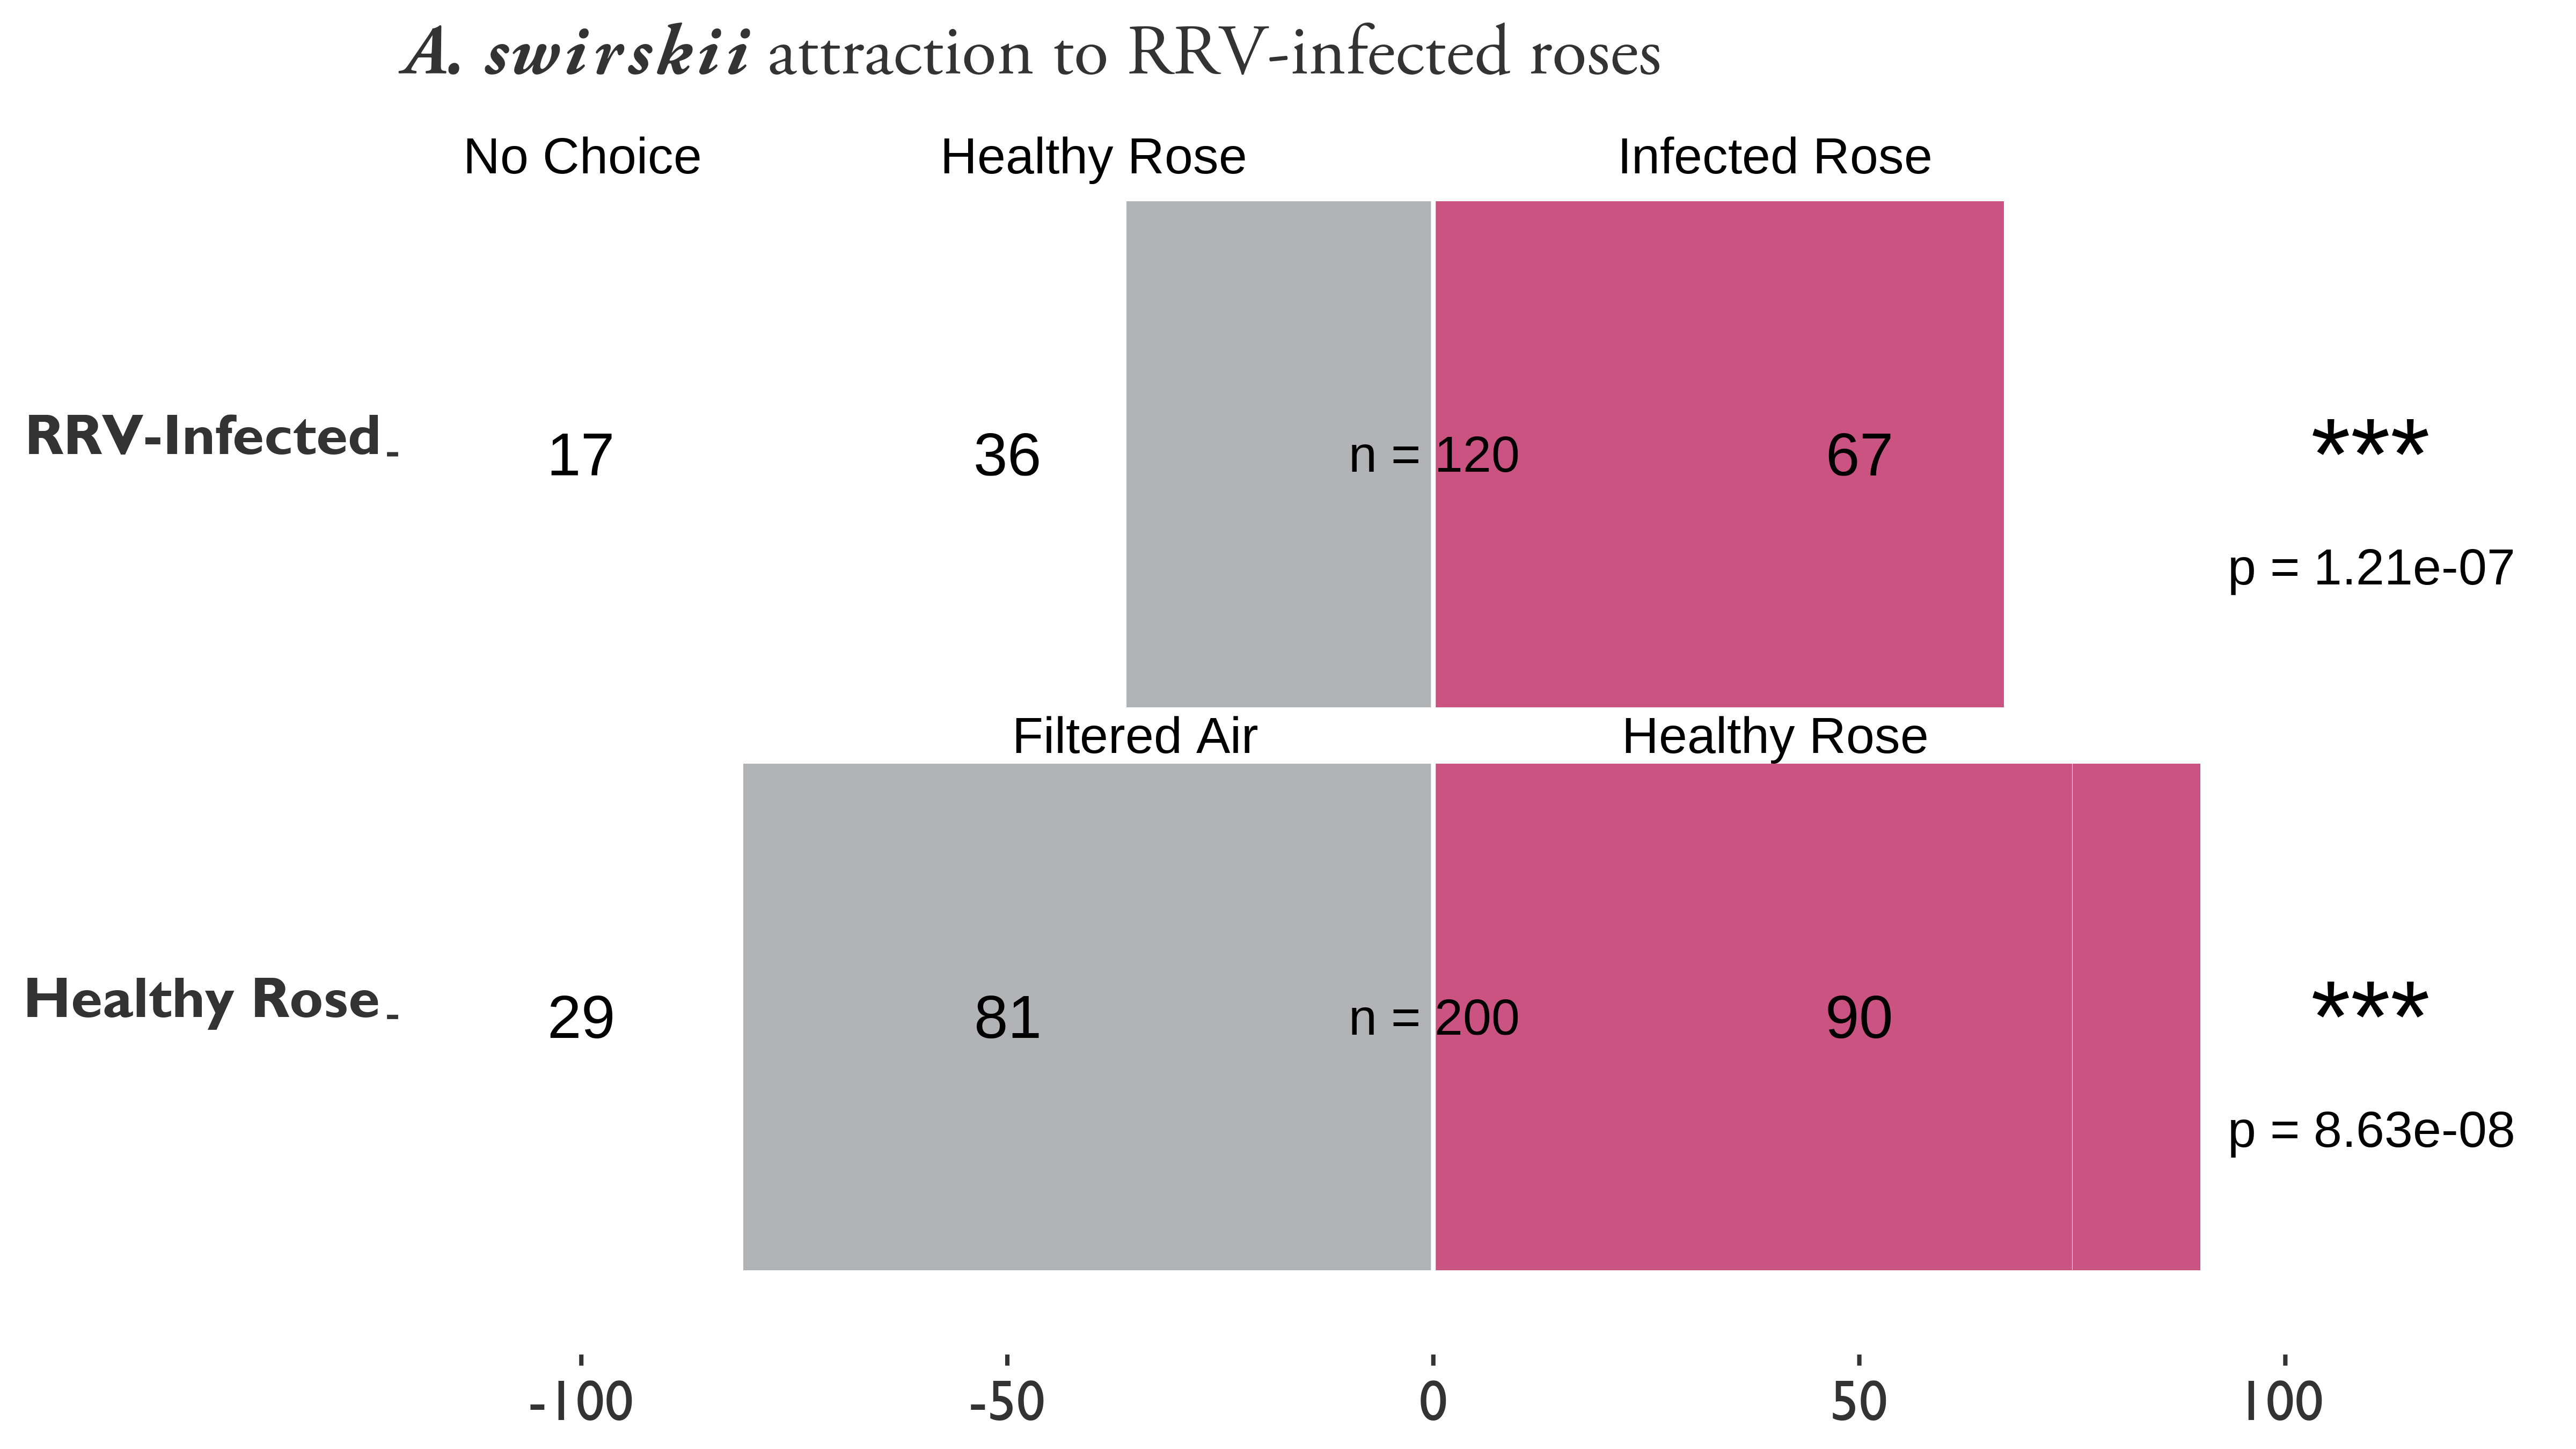
\includegraphics[width=1\linewidth]{figure/rrv_graph_olfact_rose} 

}

\caption[Attraction of the predatory phytoseiid mite \textit{Amblyseius swirskii} to healthy and Rose Rosette Virus-infected Pink Double Knock Out® roses]{\textit{Amblyseius swirskii} attraction to healthy and Rose Rosette Virus-infected Pink Double Knock Out® roses. Asterisks represent significant differences as calculated by $\chi^2$ contingency table tests for given probabilities. N.S. = not significant. RRV-infected vs Healthy Rose: $\chi^2 = 9.33$, $df = 1$, $\alpha = 0.05$, $p-value = 0.002$. Filtered Air vs Healthy Rose: $\chi^2 = 0.47$, df $=$ 1, $\alpha = 0.05$, $p-value = 0.4913$.}\label{fig:aswir-rrd}
\end{figure}
\begin{figure}

{\centering 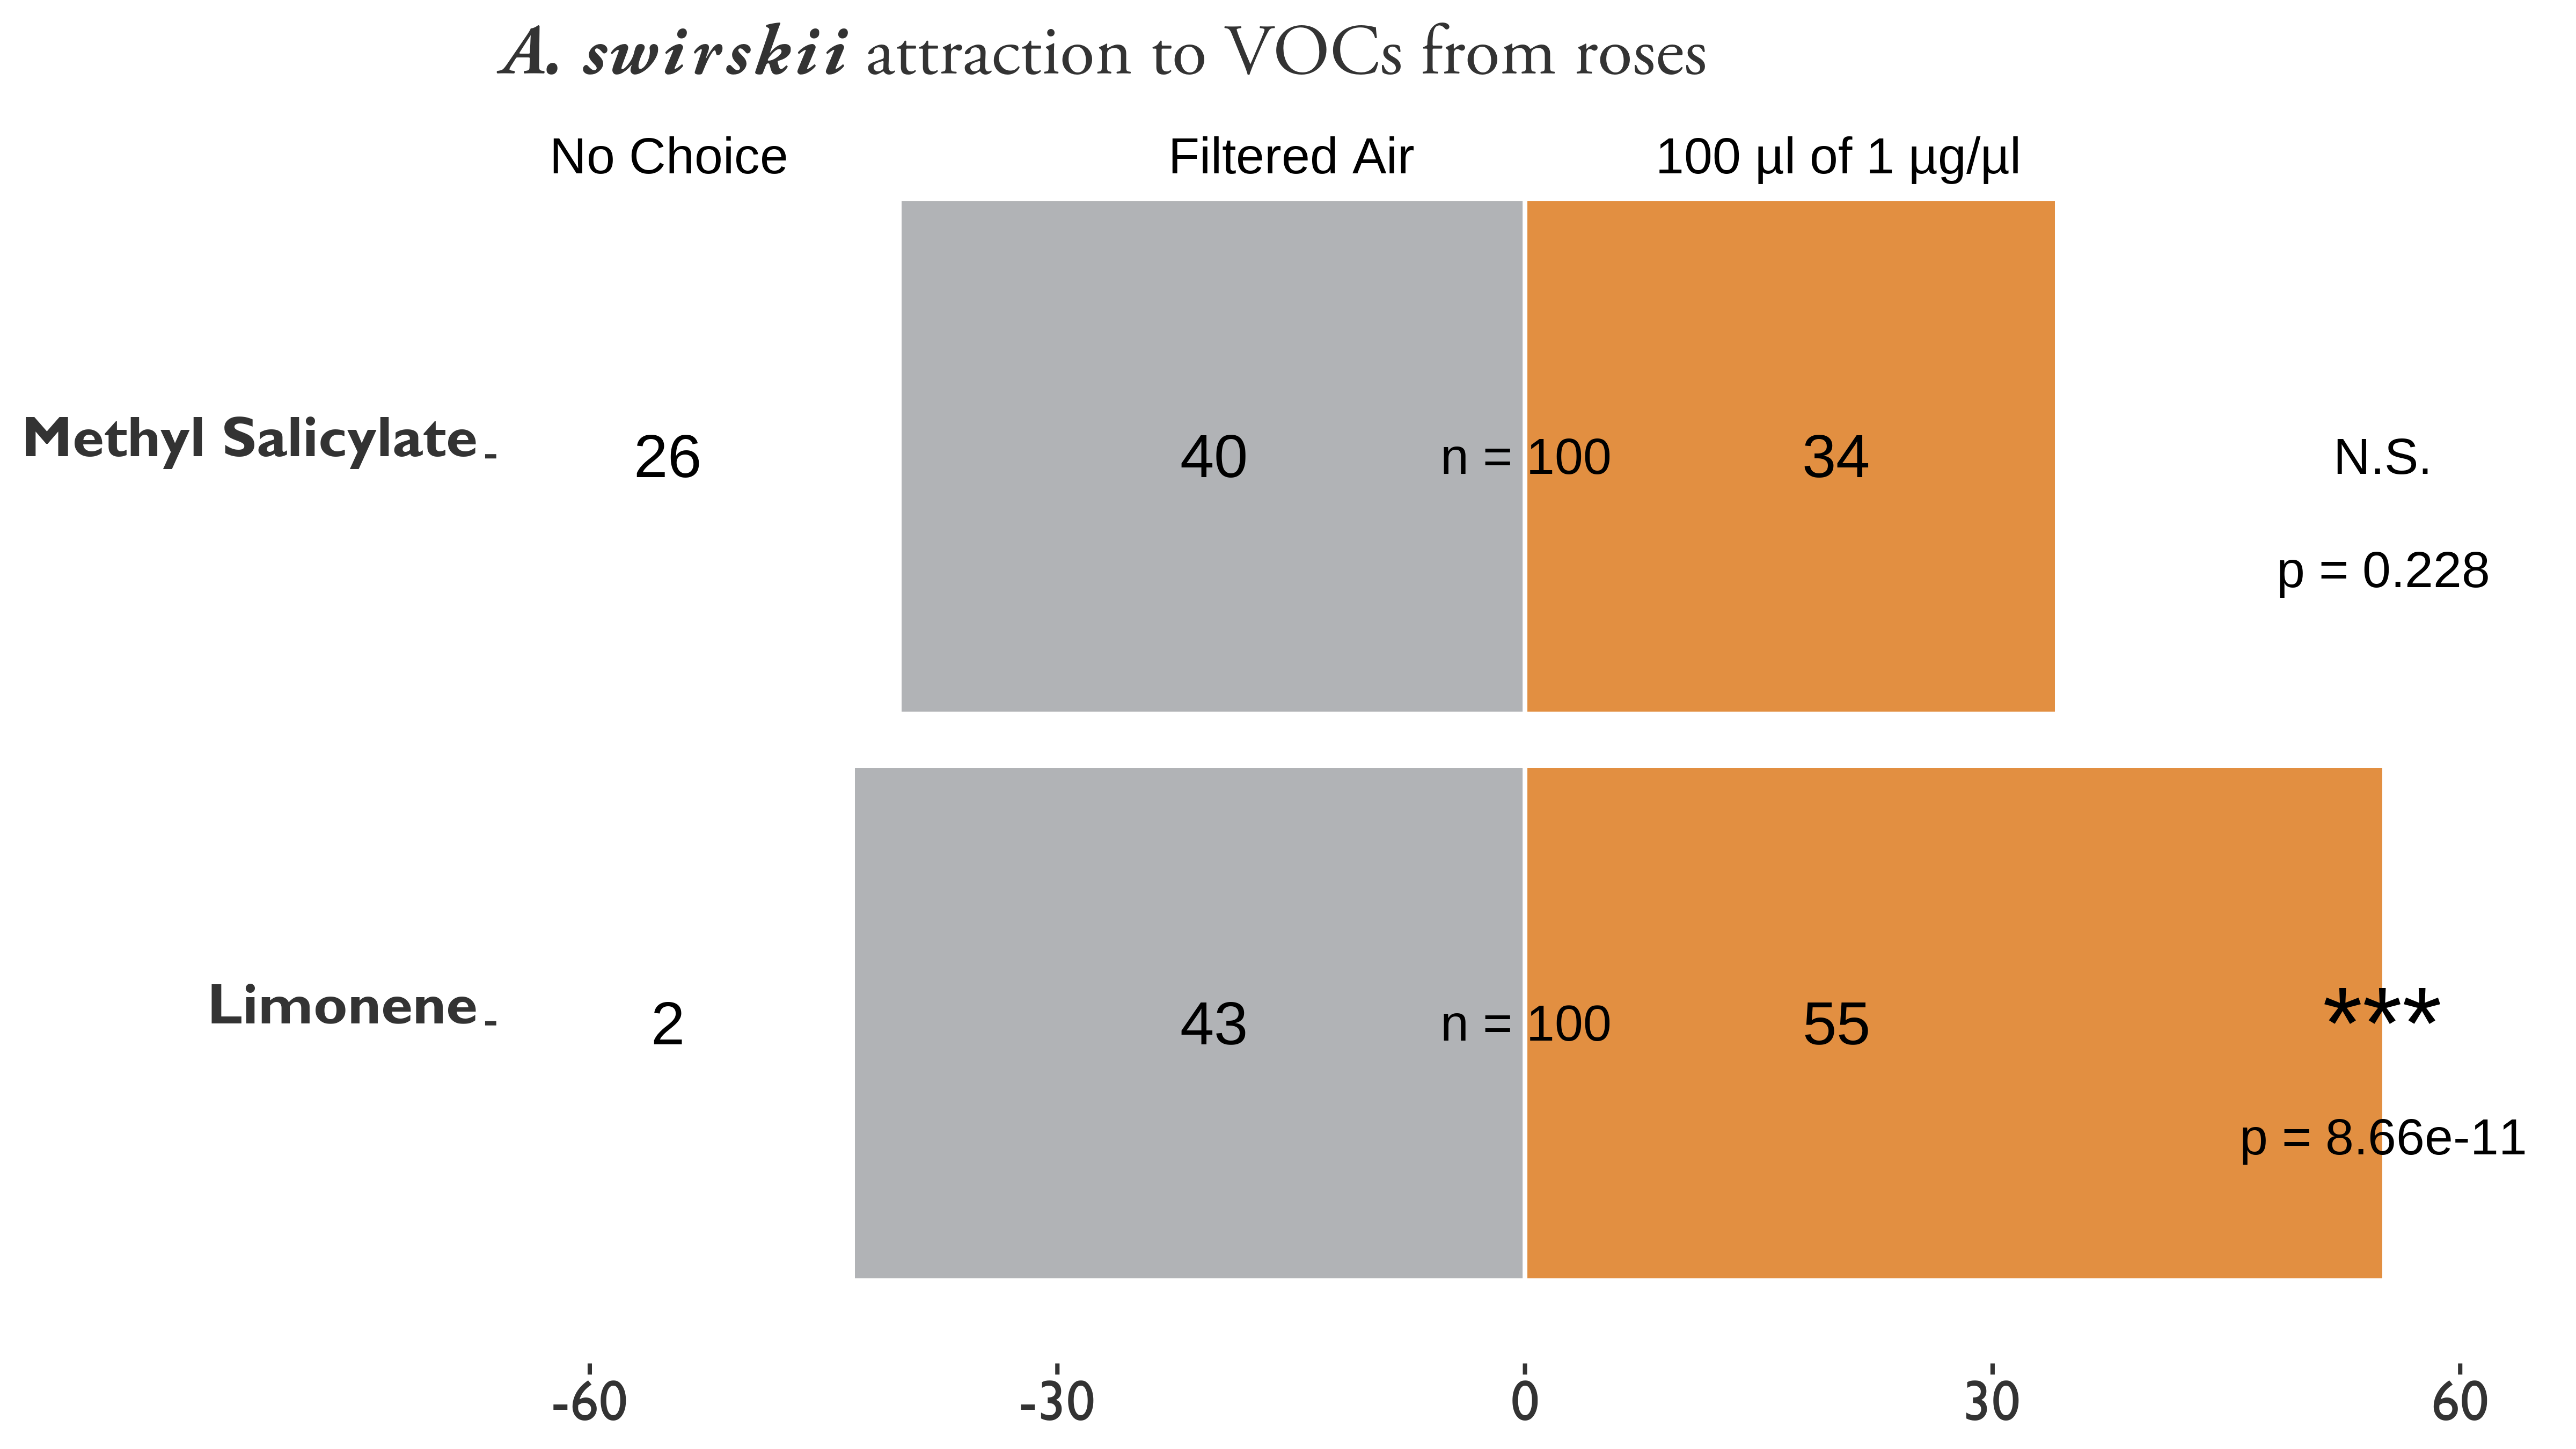
\includegraphics[width=1\linewidth]{figure/rrv_graph_olfact_vocs} 

}

\caption[\textit{Amblyseius swirskii} attraction to Methyl Salicylate (MeSA) and D-L Limonene vs filtered air]{\textit{Amblyseius swirskii} attraction to Methyl Salicylate (MeSA) and D-L Limonene vs filtered air at concentrations of 1 g/\si{\micro\liter}. 100 \si{\micro\liter}s of chemical was applied to 3 cm of dental wick inside of erlenmeyer flasks inline with the filtered air from the olfactometer. Asterisks represent significant differences as calculated by $\chi^2$ contingency table tests for given probabilities. N.S. = not significant. MeSA vs Air: $\chi^2 = 0.48649$, $df = 1$, $\alpha = 0.05$, $p-value = 0.4855$. D-L Limonene vs Air: $\chi^2 = 0.94737$, $df = 1$, $\alpha = 0.05$, $p-value = 0.3304$.}\label{fig:aswir-mesa-lim}
\end{figure}
\begin{figure}

{\centering 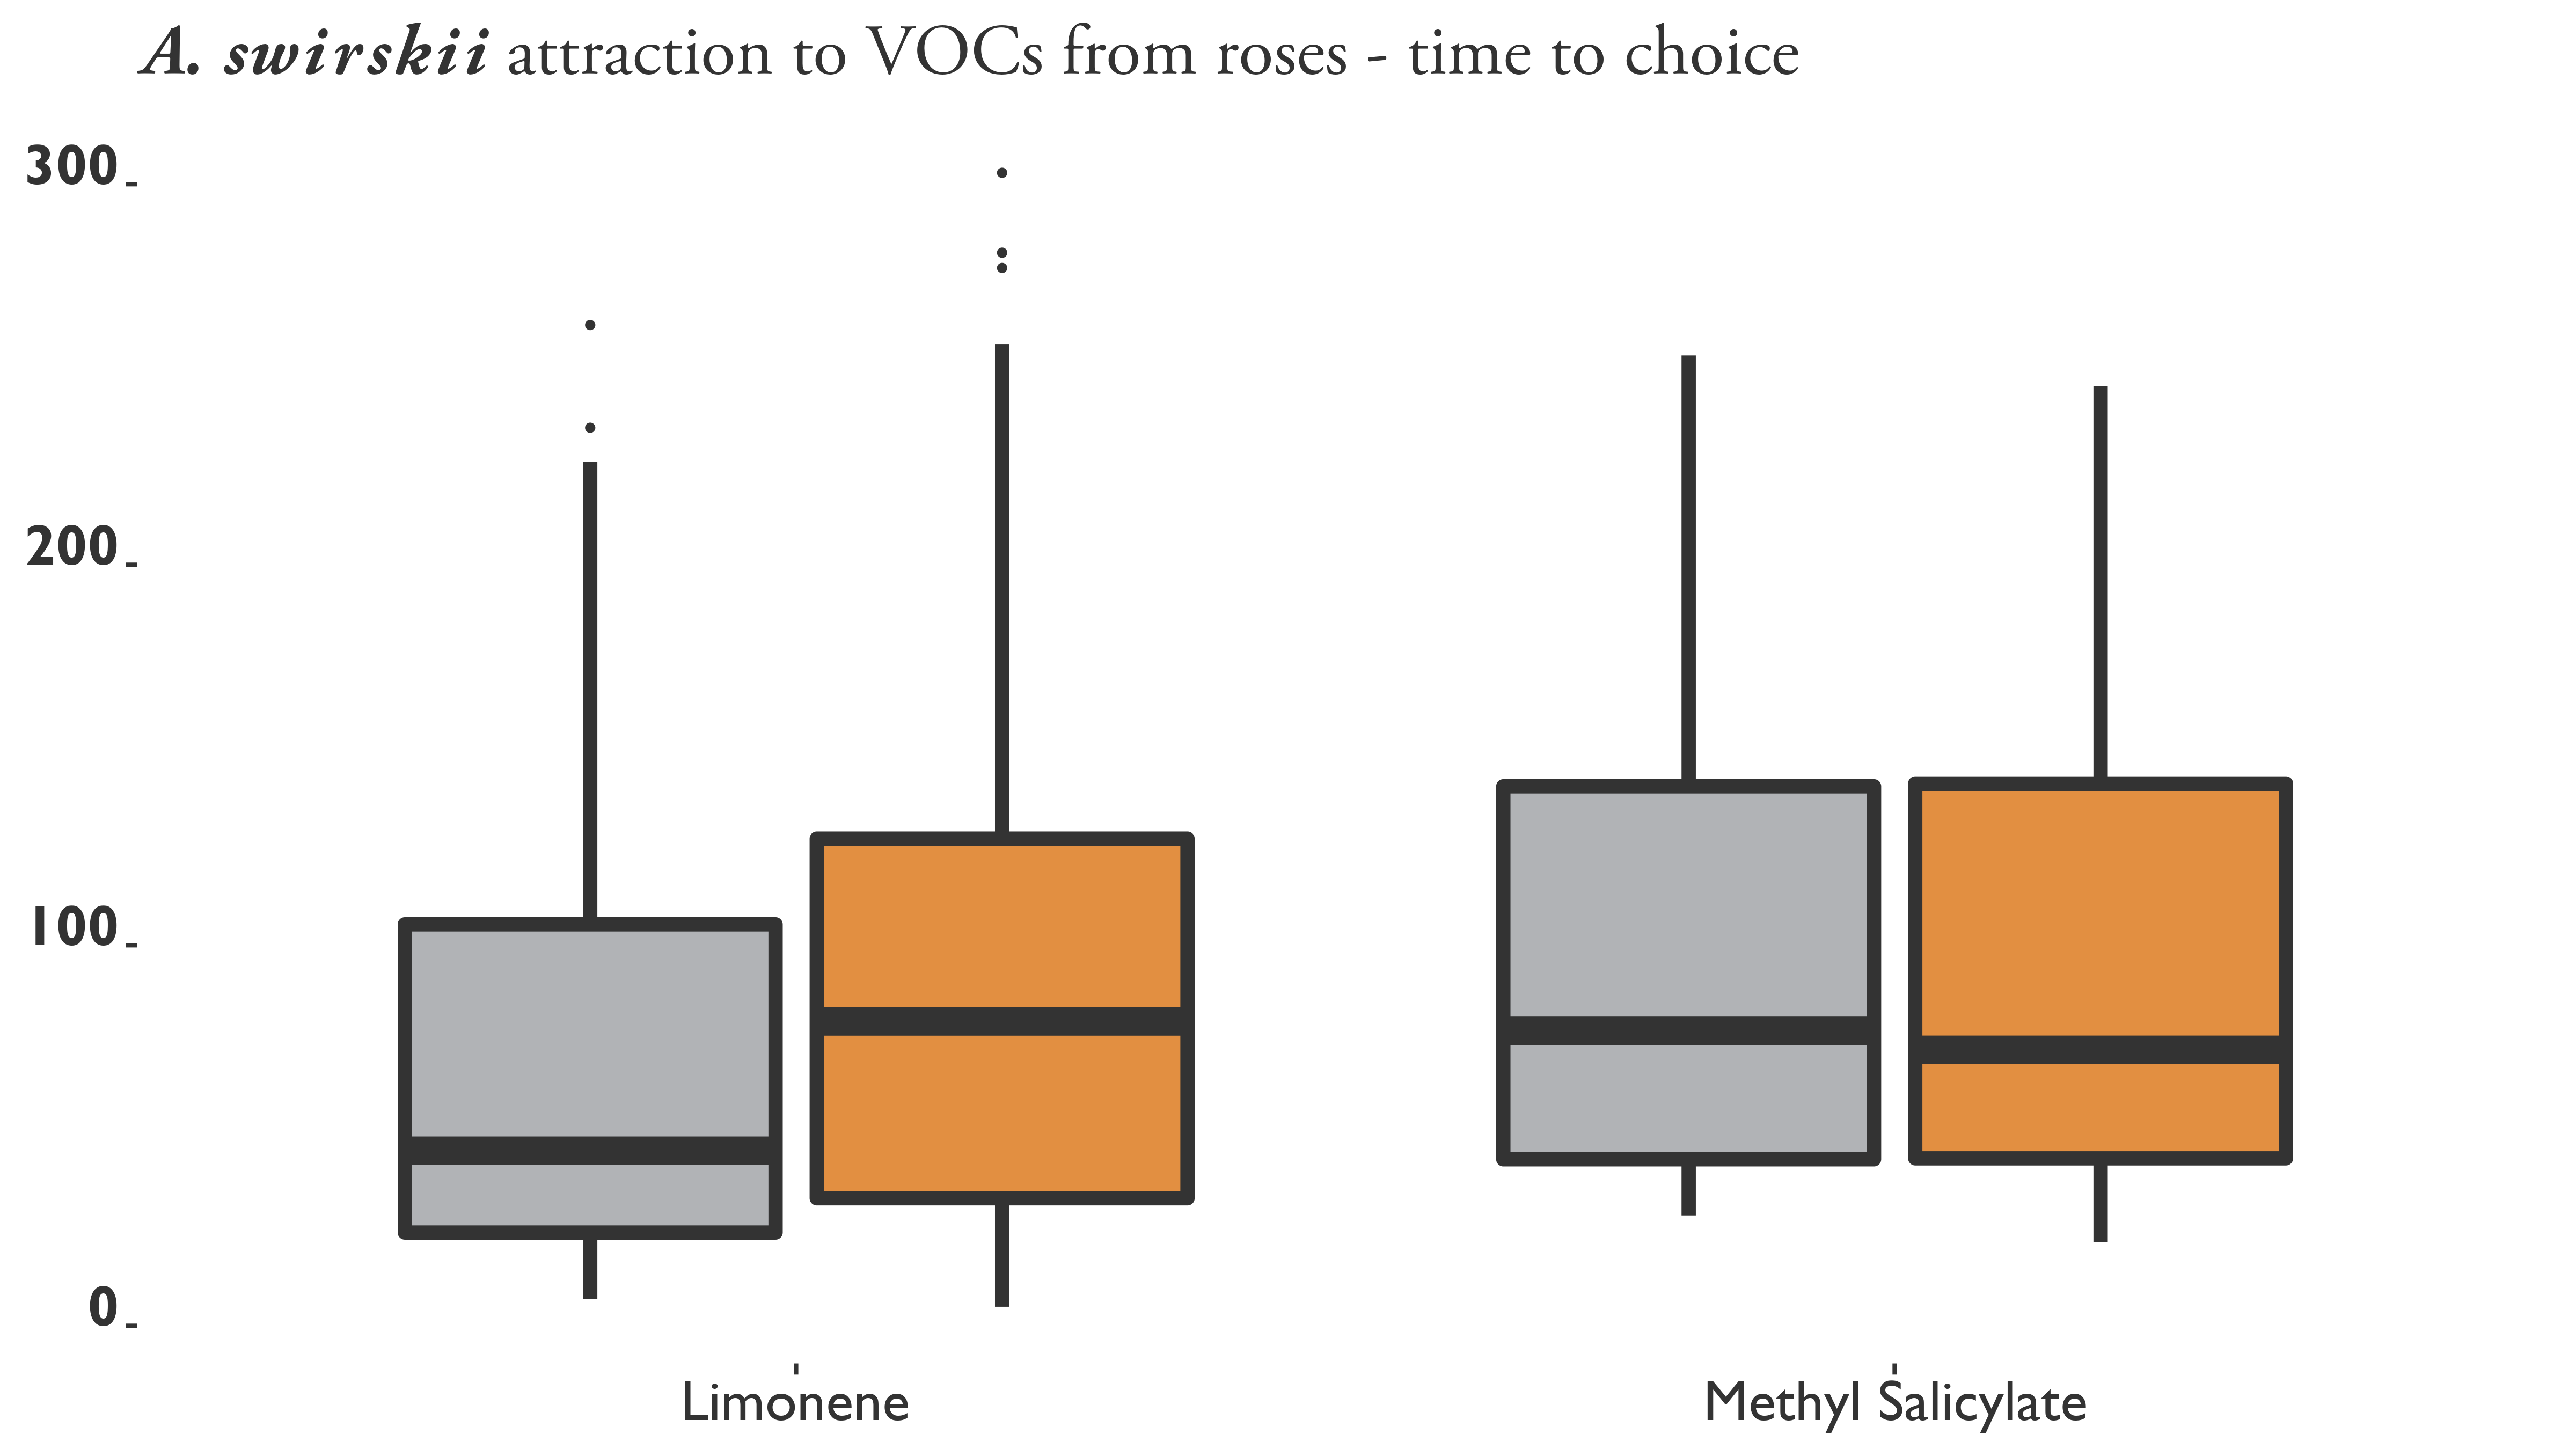
\includegraphics[width=1\linewidth]{figure/rrv_graph_olfact_vocs_time_choice} 

}

\caption[Time elapsed before choice of \textit{Amblyseius swirskii} to MeSA and D-L Limonene vs filtered air]{Time elapsed before choice of \textit{Amblyseius swirskii} to MeSA and D-L Limonene vs filtered air at concentrations of 1 g/\si{\micro\liter}. 100 \si{\micro\liter}s of chemical was applied to 3 cm of dental wick inside of erlenmeyer flasks inline with the filtered air from the olfactometer.}\label{fig:aswir-mesa-lim-times}
\end{figure}
\hypertarget{volatiles-differ-between-rrv-infected-uninfected-and-induced-roses}{%
\subsection{Volatiles differ between RRV-infected, uninfected and induced roses}\label{volatiles-differ-between-rrv-infected-uninfected-and-induced-roses}}

The top six contributing VOCs for VCTs were \textgamma-Murrolene, \textbeta-Ocimene, (E,E)-\textalpha-Farnesene, \textbeta-Caryophyllene, Methyl Salicylate and \textbeta-Pinene (\emph{\ref{tab:vcts-contrib-table}}). The top six contributing chemicals for SPME were \textgamma-Murrolene, \textbeta-Caryophyllene 1R-\textalpha-Pinene, Mesitylene, \textbeta-Pinene and m-Xylene (\emph{\ref{tab:spme-contrib-table}}). Roses infected with RRD were generally similar to uninfected roses for both VCT and SPME methods, (\emph{\ref{fig:vcts-vocs-compares}}, \emph{\ref{fig:spme-vocs-compares}}, \emph{\ref{fig:vcts-vocs-umap}}, \emph{\ref{fig:spme-vocs-umap}}), but ASM-treated roses had less chemical variance than either group (\emph{\ref{fig:spme-vocs-compares}}, \emph{\ref{fig:spme-vocs-umap}}). For VCT samples, \textgamma-Murrolene explained most of the variance in uninfected roses, while SPME samples showed the opposite:\textgamma-Murrolene and \textbeta-Caryophyllene were primarily found in infected roses.
\begin{figure}

{\centering 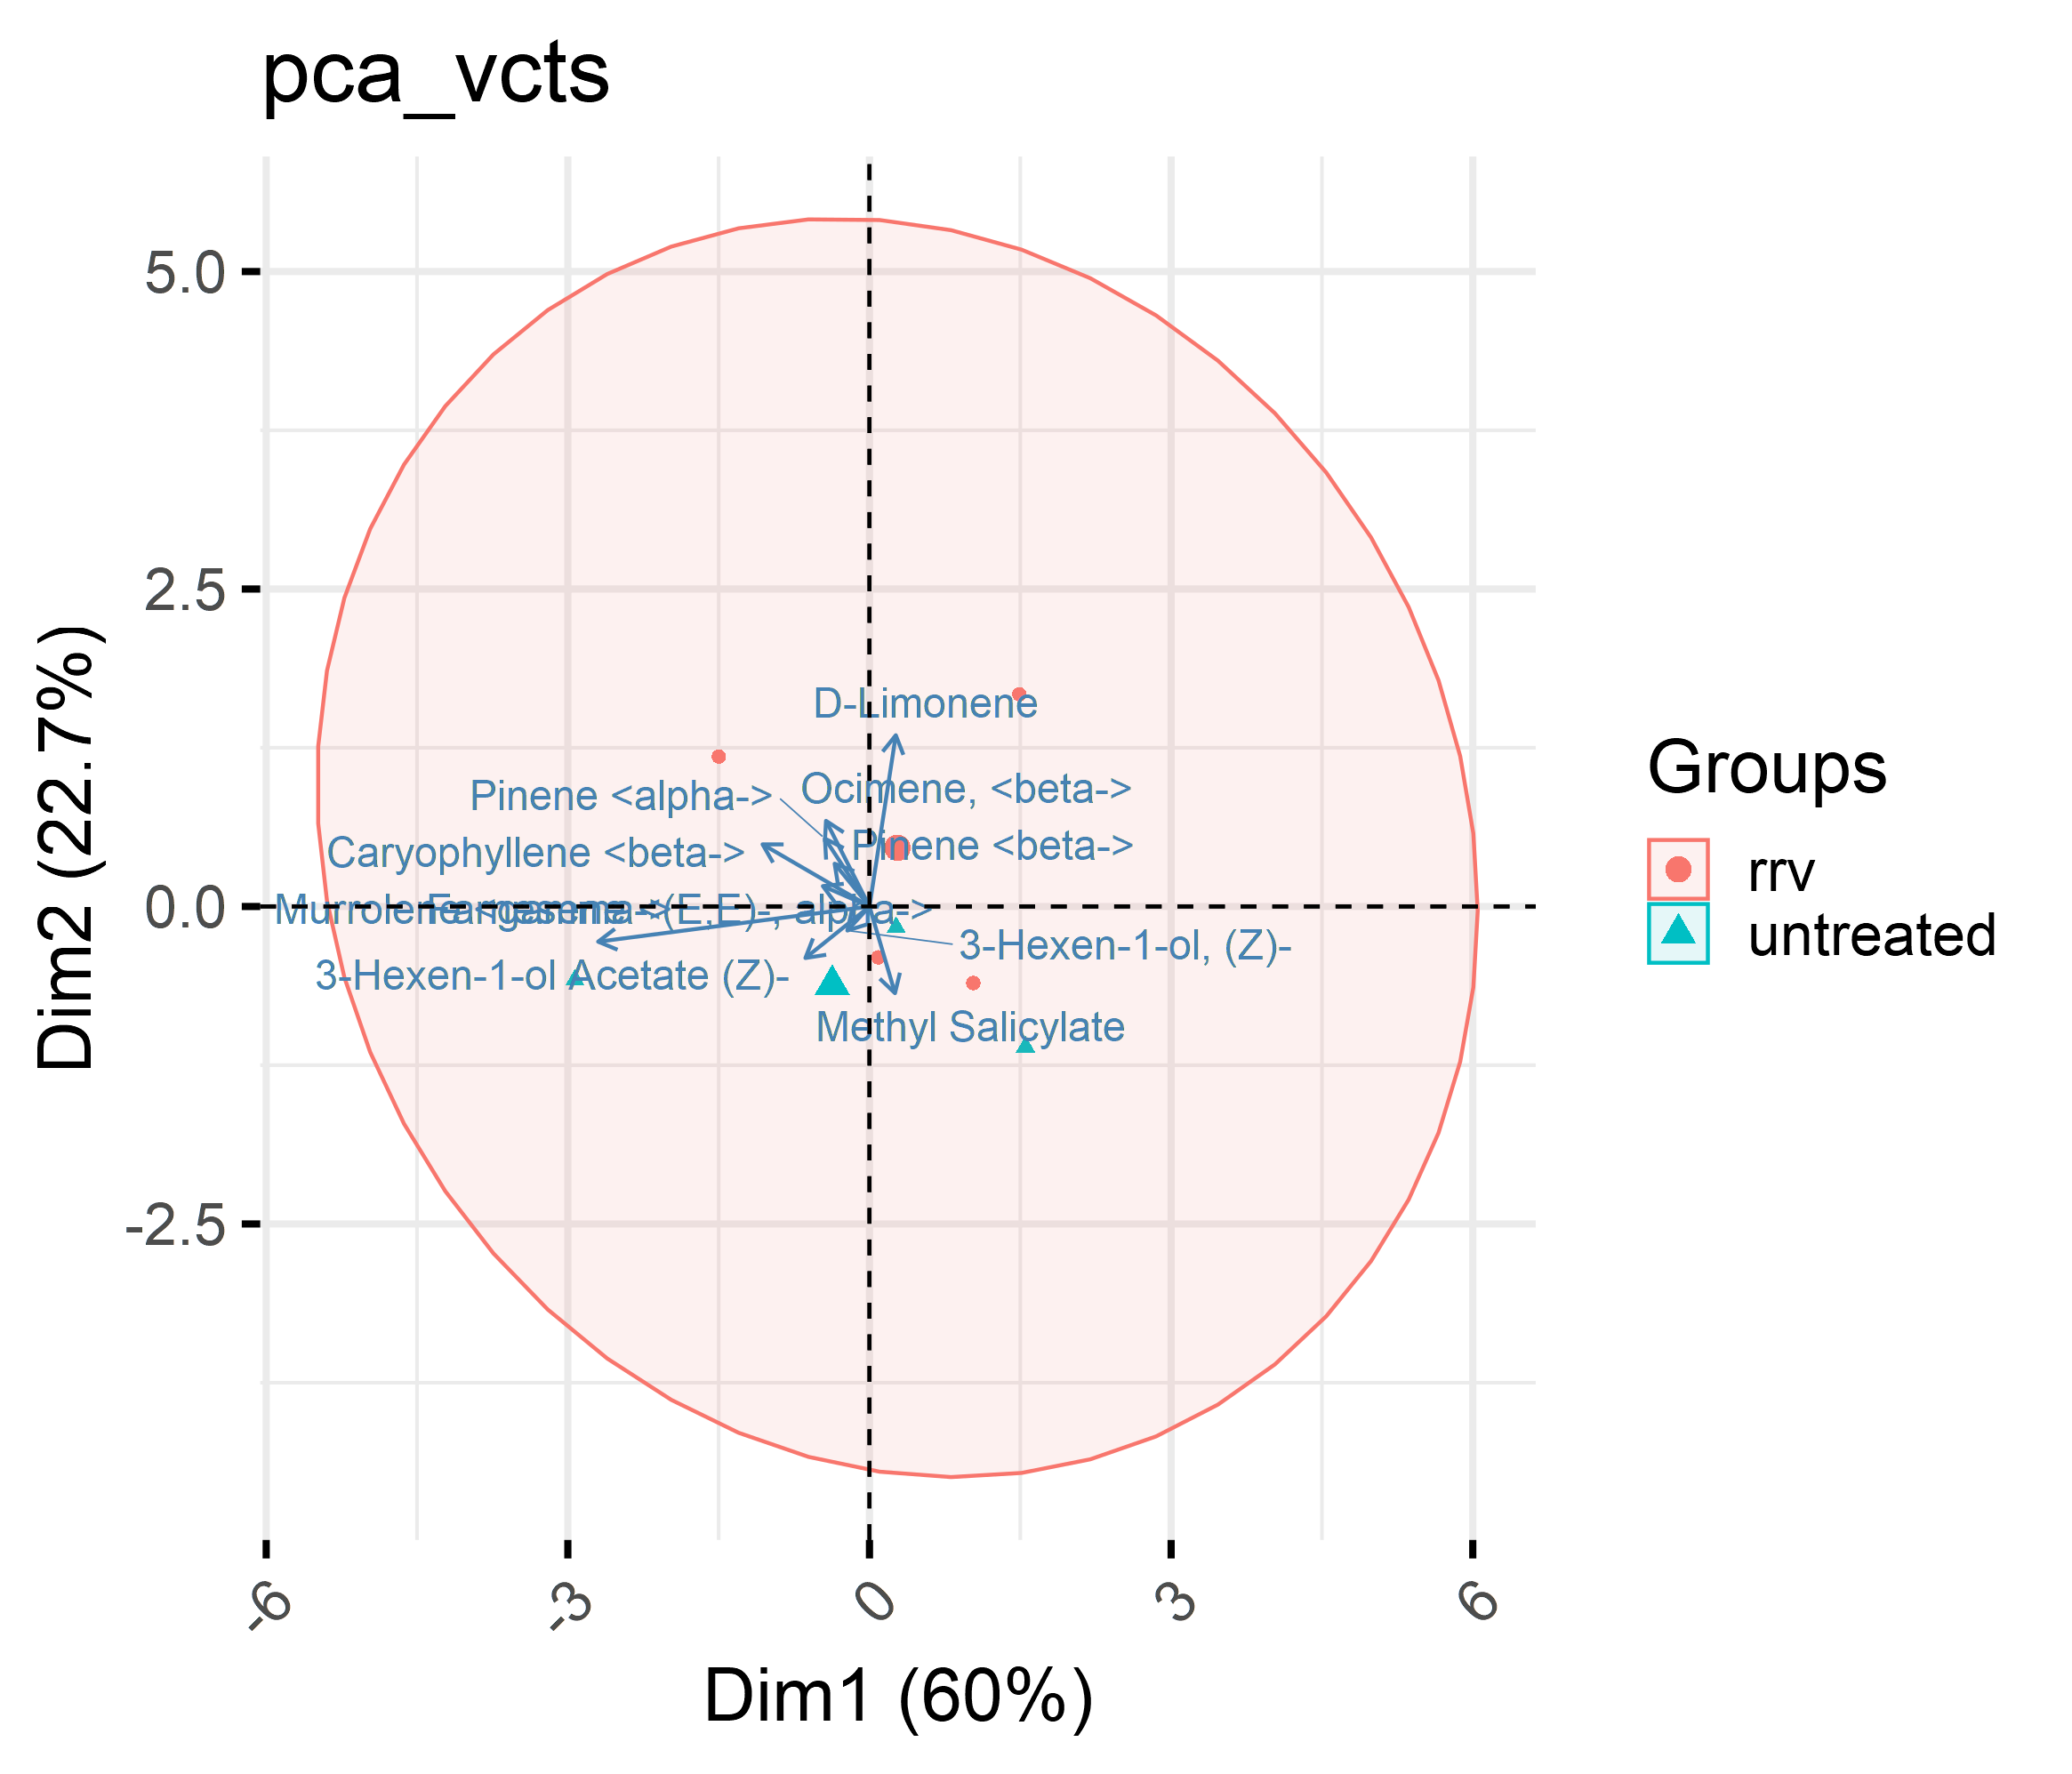
\includegraphics[width=1.1\linewidth]{figure/rrv_volatiles_pca_var_biplot_pca_vcts} 

}

\caption[Principal component analysis (PCA) biplot of volatiles collected with Volatile Collection Traps (VCTs)]{Principal component analysis (PCA) biplot of volatiles collected with Volatile Collection Traps (VCTs). Ellipses represent 95\% confidence intervals. Clusters represent similarities in chemical profile.}\label{fig:vcts-vocs-compares}
\end{figure}
\begin{figure}

{\centering 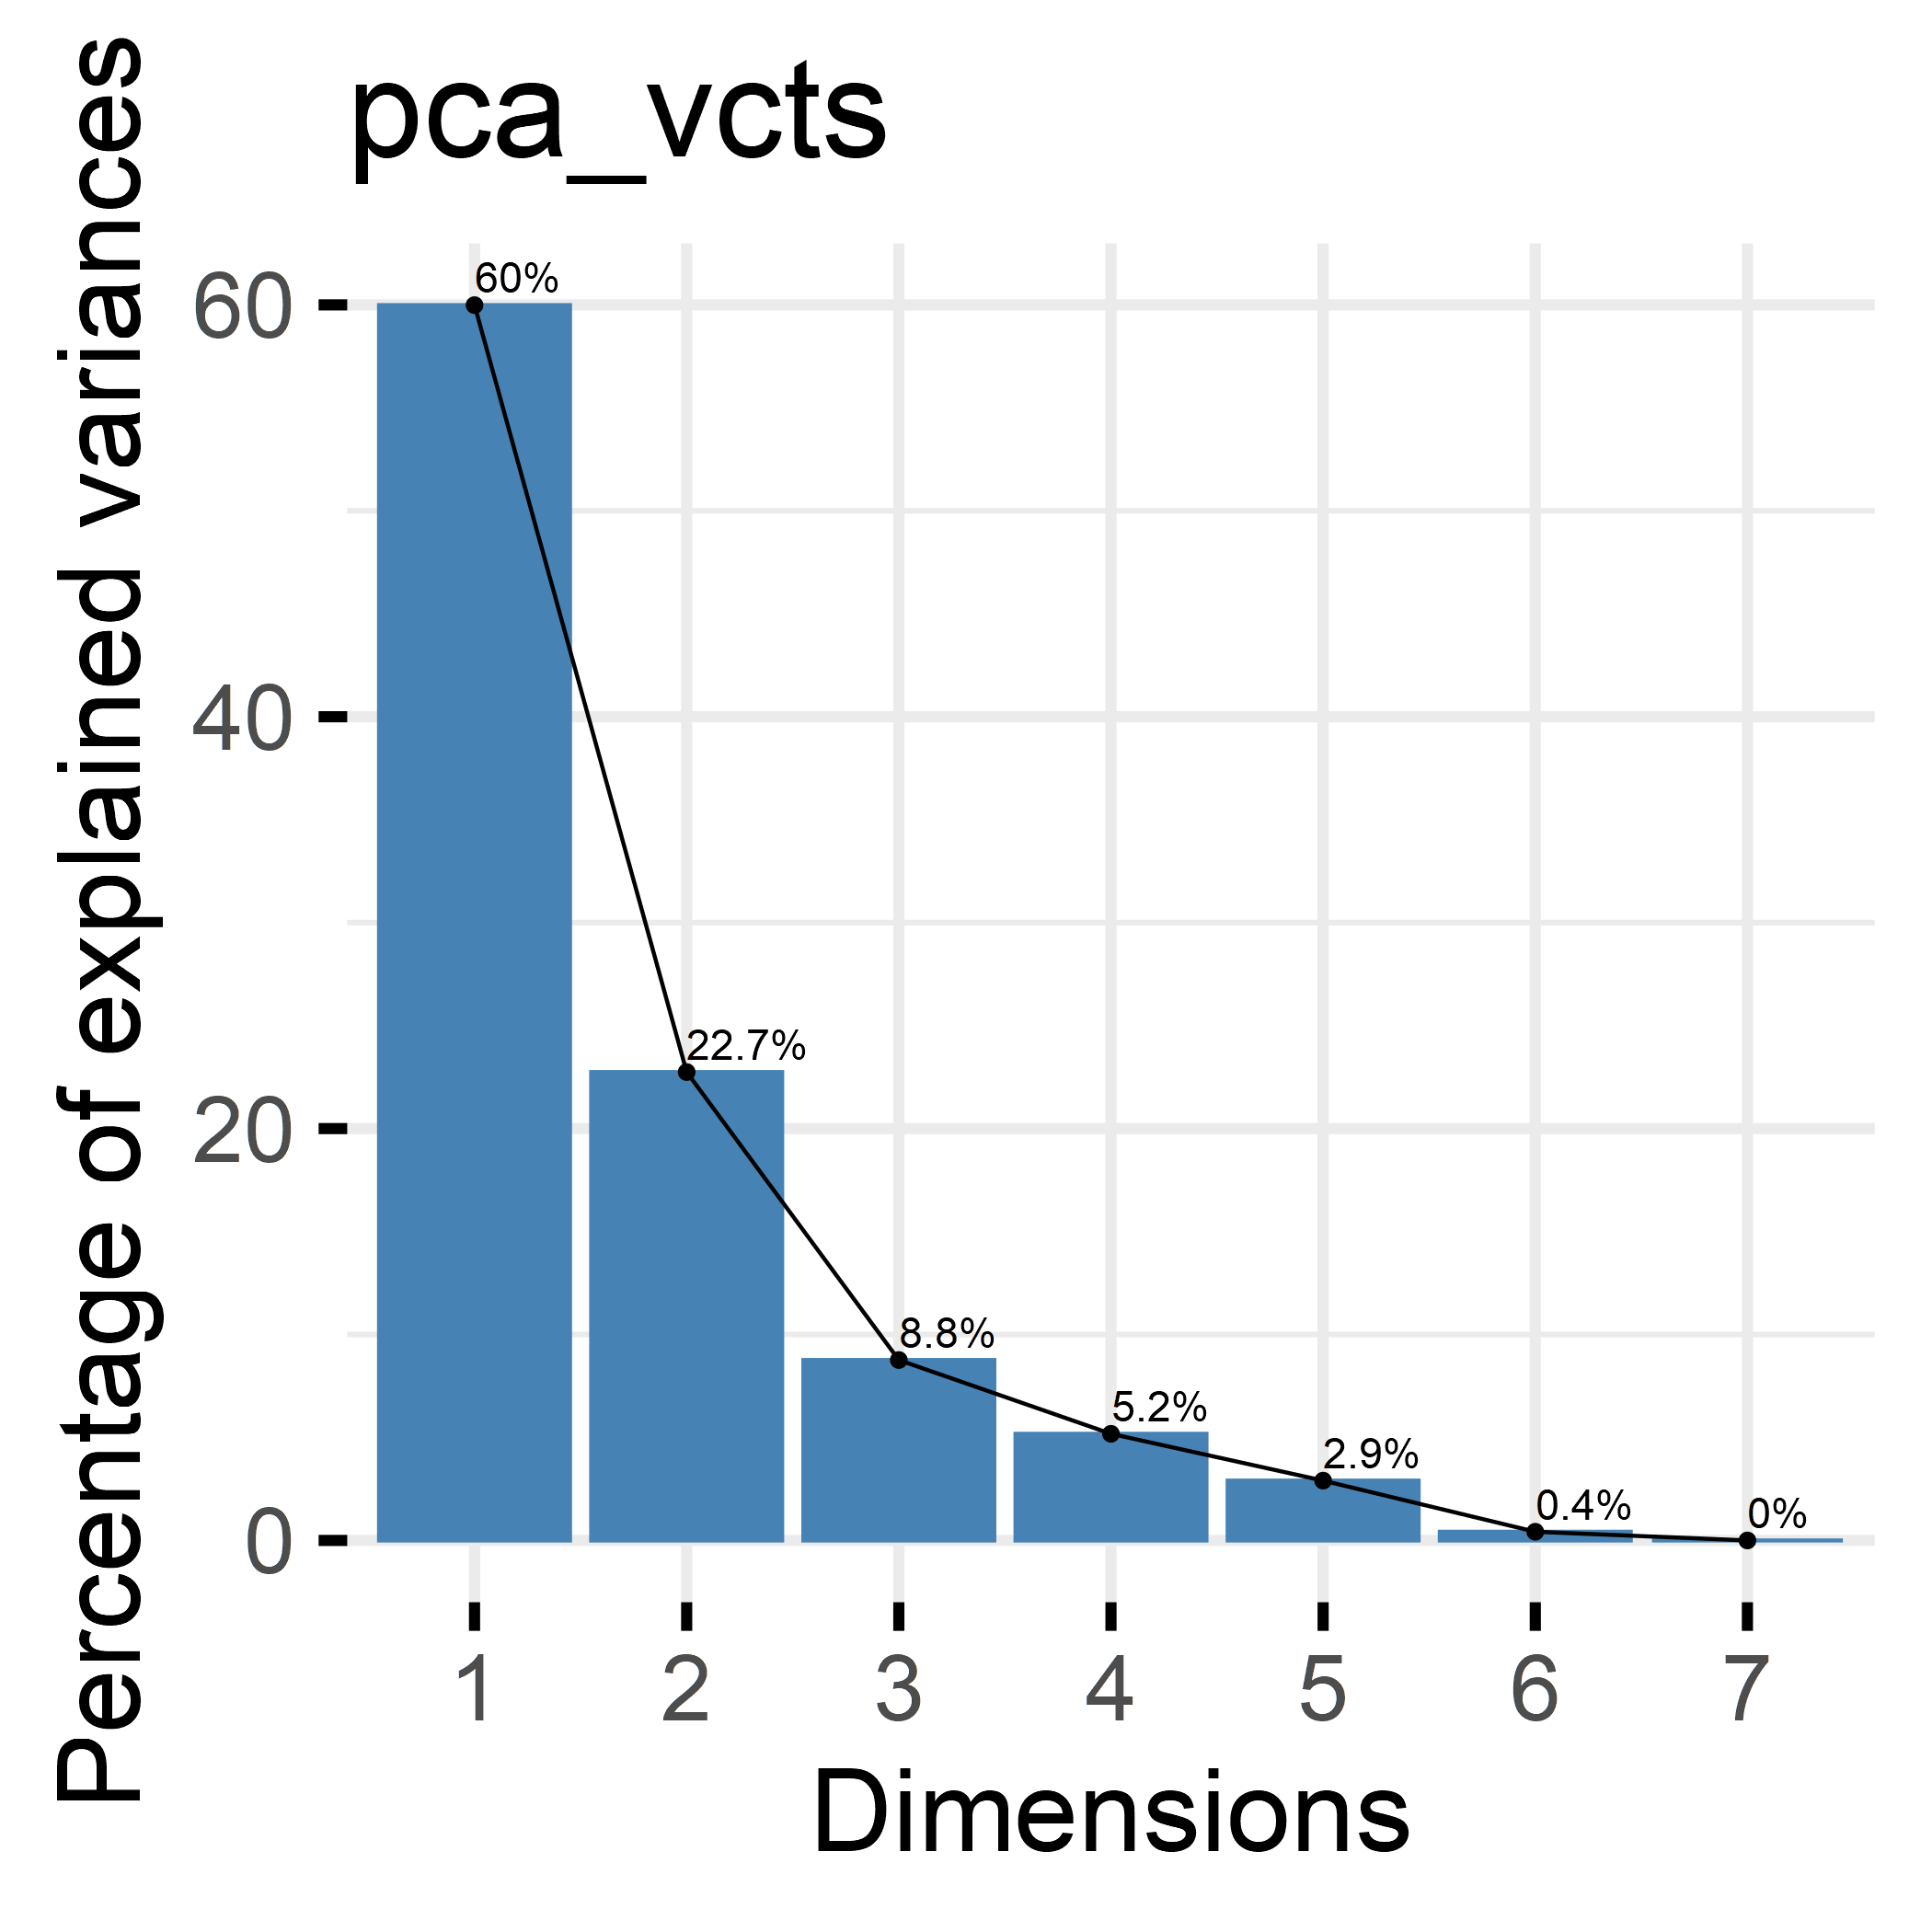
\includegraphics[width=1\linewidth]{figure/rrv_volatiles_screeplot_pca_vcts} 

}

\caption[Scree plot of VCT principal components]{Scree plot of VCT principal components.}\label{fig:vcts-vocs-scree}
\end{figure}
\begin{figure}

{\centering 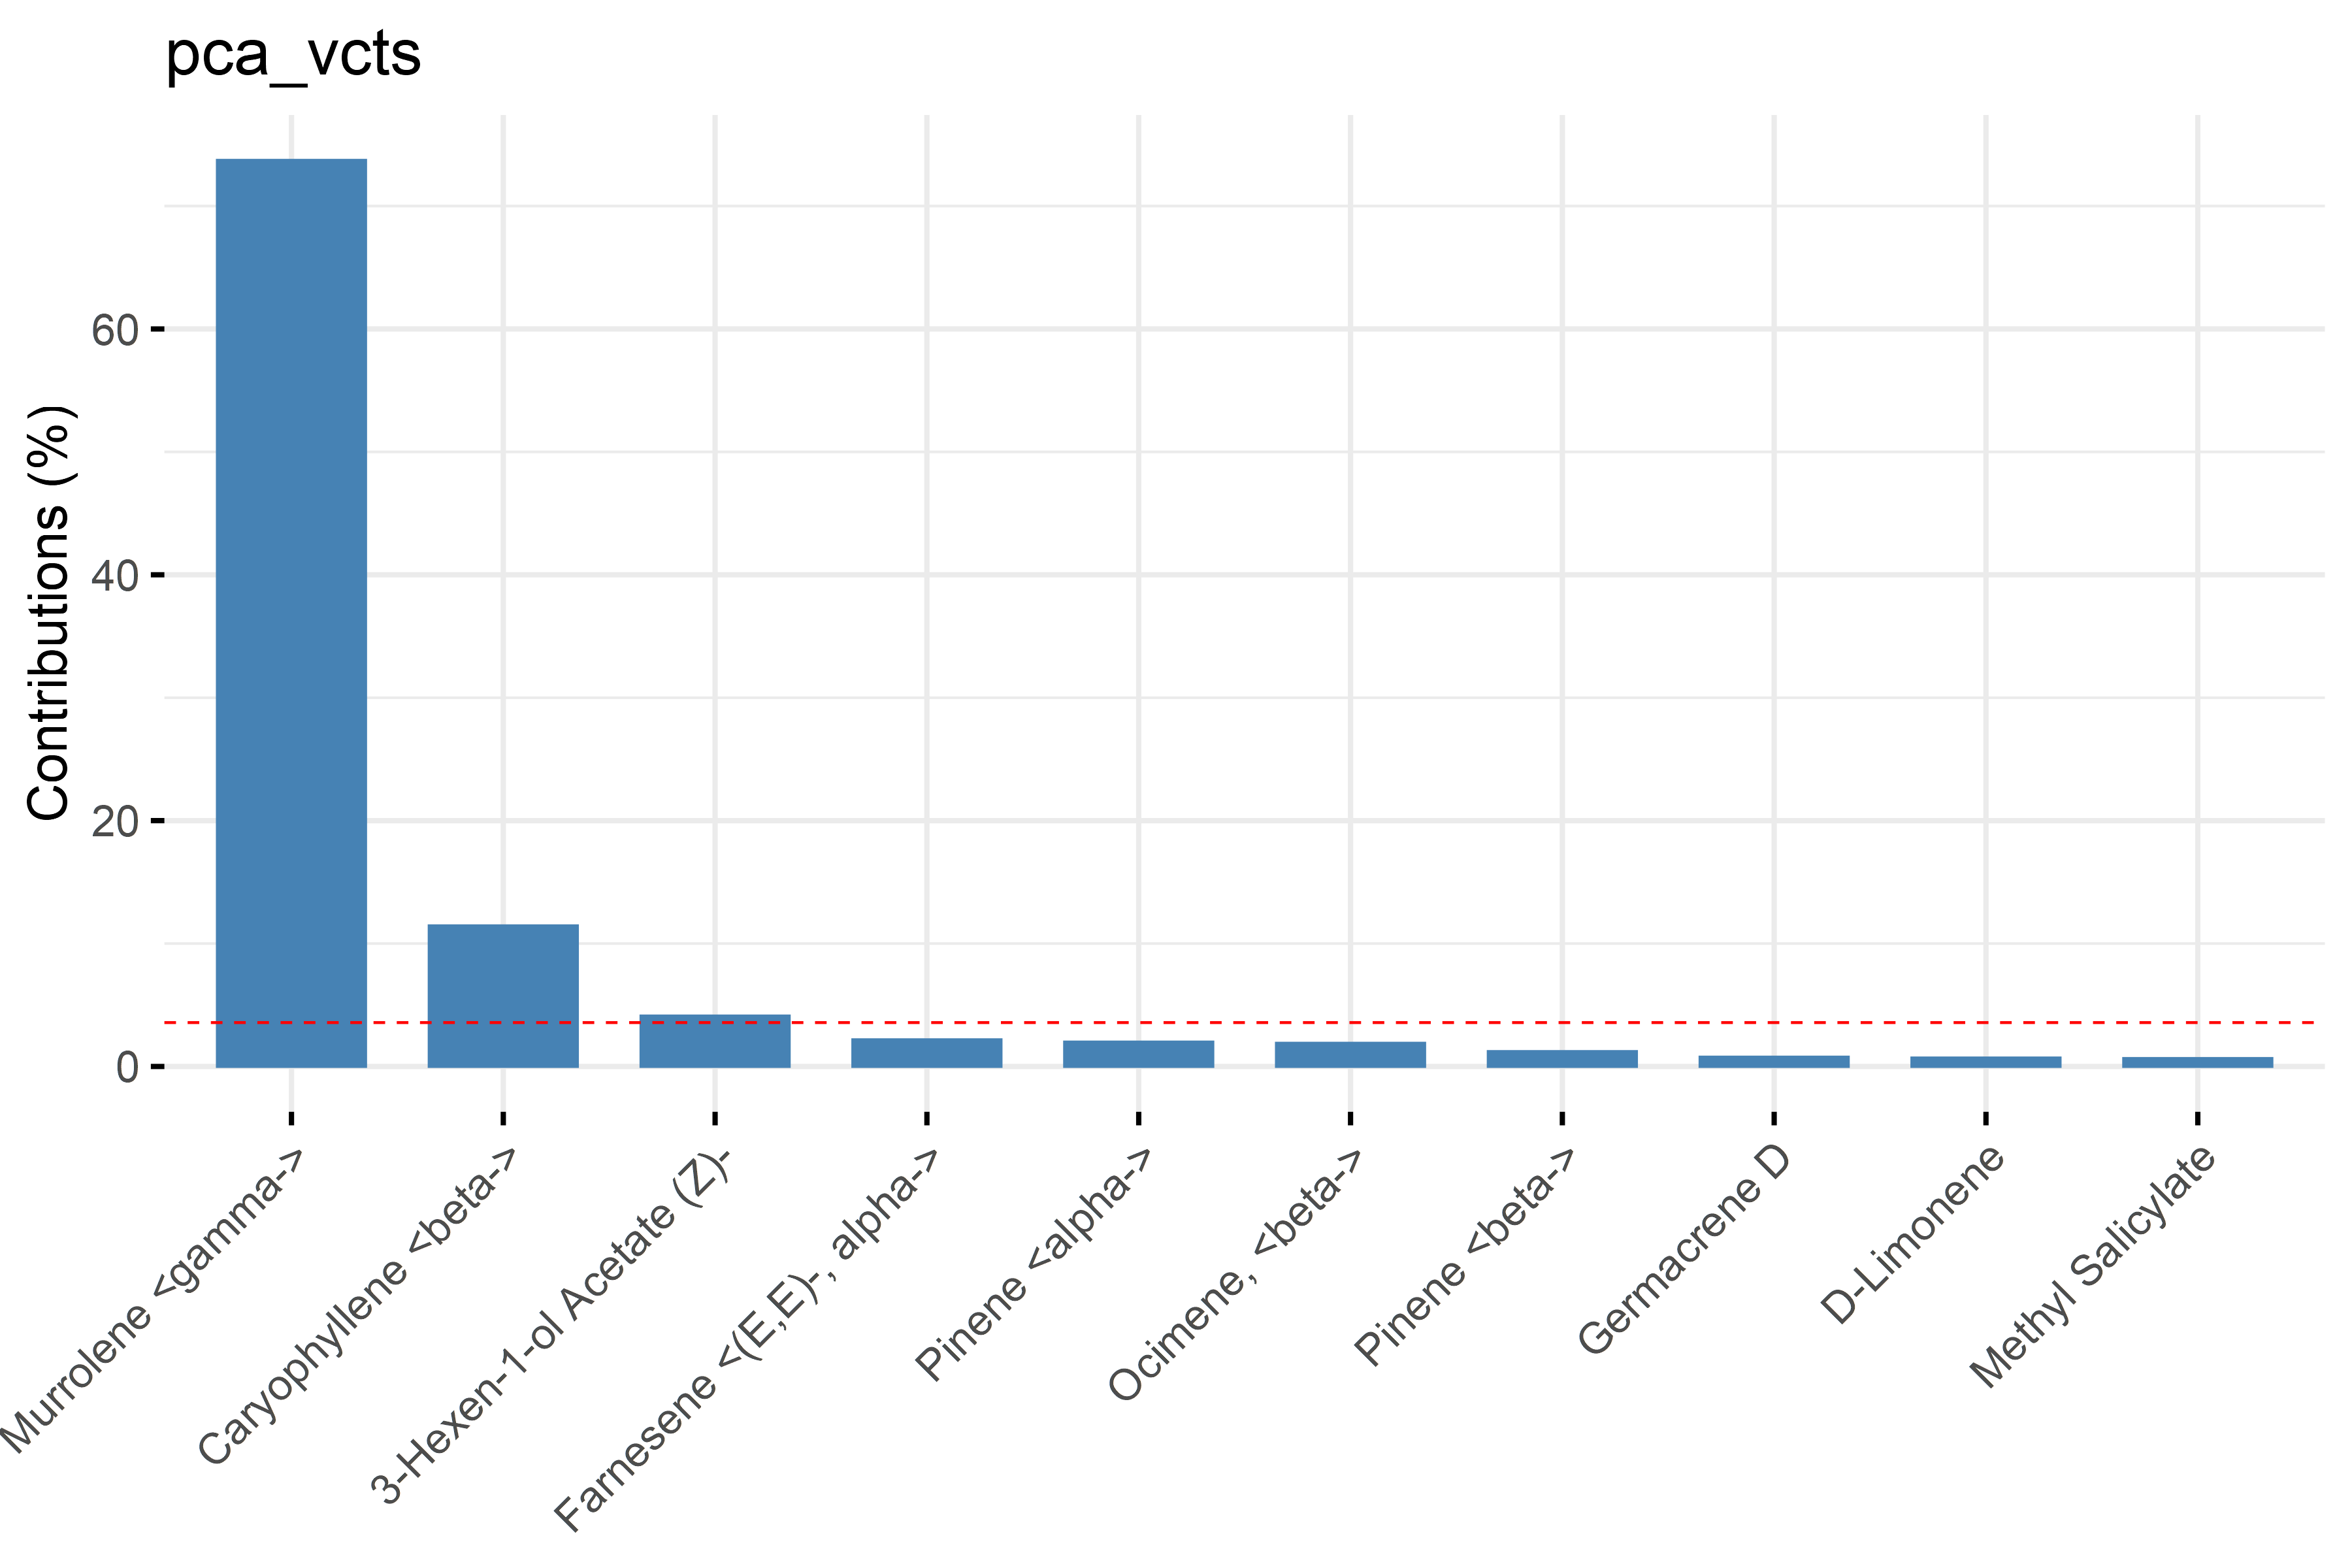
\includegraphics[width=1\linewidth]{figure/rrv_volatiles_var_pca_vcts} 

}

\caption[Top ten contributing volatiles collected with the VCT method as determined by PCA.]{Top ten contributing volatiles collected with the VCT method as determined by PCA.}\label{fig:vcts-vocs}
\end{figure}
\begin{table}

\caption{\label{tab:vcts-contrib-table}Contribution table for PCA of headspace VOCs collected with VCT methods from Pink Double Knock Out® roses.}
\centering
\resizebox{\linewidth}{!}{
\begin{tabular}[t]{lrrr}
\toprule
Chemical & PCA1 & PCA2 & PCA3\\
\midrule
\cellcolor{gray!6}{Murrolene <gamma->} & \cellcolor{gray!6}{73.7200281} & \cellcolor{gray!6}{2.0505736} & \cellcolor{gray!6}{0.0590805}\\
Caryophyllene <beta-> & 11.4442072 & 6.3932415 & 1.6136116\\
\cellcolor{gray!6}{3-Hexen-1-ol Acetate (Z)-} & \cellcolor{gray!6}{4.1088721} & \cellcolor{gray!6}{4.3938742} & \cellcolor{gray!6}{0.0543187}\\
Farnesene <(E,E)-, alpha-> & 2.1748819 & 0.6870580 & 1.2212043\\
\cellcolor{gray!6}{Pinene <alpha->} & \cellcolor{gray!6}{1.9893868} & \cellcolor{gray!6}{7.6247823} & \cellcolor{gray!6}{1.5809223}\\
\addlinespace
Ocimene, <beta-> & 1.8922159 & 12.1385950 & 3.3711482\\
\cellcolor{gray!6}{Pinene <beta->} & \cellcolor{gray!6}{1.2158051} & \cellcolor{gray!6}{3.0295147} & \cellcolor{gray!6}{1.3808570}\\
Germacrene D & 0.7637065 & 0.0169593 & 0.0005140\\
\cellcolor{gray!6}{D-Limonene} & \cellcolor{gray!6}{0.6934082} & \cellcolor{gray!6}{48.5442320} & \cellcolor{gray!6}{4.7360377}\\
Methyl Salicylate & 0.6511928 & 12.4348187 & 84.5744765\\
\addlinespace
\cellcolor{gray!6}{3-Hexen-1-ol, (Z)-} & \cellcolor{gray!6}{0.4892346} & \cellcolor{gray!6}{0.9571750} & \cellcolor{gray!6}{0.1575944}\\
Cadinene <delta-> & 0.1804902 & 0.1066432 & 0.2043152\\
\cellcolor{gray!6}{Nona-1,3,7-triene <4-8-dimethyl-, (E)->} & \cellcolor{gray!6}{0.1485550} & \cellcolor{gray!6}{0.0001213} & \cellcolor{gray!6}{0.0034408}\\
2-Hexenal & 0.1396463 & 0.0379478 & 0.0191767\\
\cellcolor{gray!6}{Copaene <beta->} & \cellcolor{gray!6}{0.1250792} & \cellcolor{gray!6}{0.0000533} & \cellcolor{gray!6}{0.0895675}\\
\addlinespace
Humulene & 0.0717575 & 0.0196316 & 0.0003570\\
\cellcolor{gray!6}{Aromadendrene} & \cellcolor{gray!6}{0.0486886} & \cellcolor{gray!6}{0.1419599} & \cellcolor{gray!6}{0.2551968}\\
2,4,6-Octatriene, 2,6-dimethyl-, (E,Z)- & 0.0352002 & 0.0348526 & 0.0458192\\
\cellcolor{gray!6}{Calamenene} & \cellcolor{gray!6}{0.0292478} & \cellcolor{gray!6}{0.1013612} & \cellcolor{gray!6}{0.3343829}\\
Caryophyllene <9-epi-(E)-> & 0.0238007 & 0.1026956 & 0.0680314\\
\addlinespace
\cellcolor{gray!6}{Ocimene, <trans-beta->} & \cellcolor{gray!6}{0.0200925} & \cellcolor{gray!6}{0.0135288} & \cellcolor{gray!6}{0.0222477}\\
Nerolidol & 0.0126271 & 0.0034313 & 0.0017340\\
\cellcolor{gray!6}{2-Hexen-1-ol, acetate, (E)-} & \cellcolor{gray!6}{0.0093561} & \cellcolor{gray!6}{0.0819047} & \cellcolor{gray!6}{0.0016911}\\
Pentane, 3-ethyl-2,2-dimethyl- & 0.0051438 & 0.0121933 & 0.0941394\\
\cellcolor{gray!6}{Myrcene <beta->} & \cellcolor{gray!6}{0.0029627} & \cellcolor{gray!6}{0.1348161} & \cellcolor{gray!6}{0.0120437}\\
\addlinespace
Trivertal & 0.0027171 & 0.2966634 & 0.0007833\\
\cellcolor{gray!6}{2-Thujene} & \cellcolor{gray!6}{0.0013261} & \cellcolor{gray!6}{0.0817092} & \cellcolor{gray!6}{0.0081560}\\
5-Hepten-2-one, <6-methyl-> & 0.0003697 & 0.5596623 & 0.0891524\\
\bottomrule
\end{tabular}}
\end{table}
\begin{table}

\caption{\label{tab:vcts-corr-table}Correlation table for PCA of headspace VOCs collected with VCT methods from Pink Double Knock Out® roses.}
\centering
\resizebox{\linewidth}{!}{
\begin{tabular}[t]{lrrr}
\toprule
Chemical & PCA1 & PCA2 & PCA3\\
\midrule
\cellcolor{gray!6}{D-Limonene} & \cellcolor{gray!6}{0.1385033} & \cellcolor{gray!6}{0.7135872} & \cellcolor{gray!6}{0.1383390}\\
Methyl Salicylate & 0.1342210 & -0.3611586 & 0.5845971\\
\cellcolor{gray!6}{Calamenene} & \cellcolor{gray!6}{0.0284454} & \cellcolor{gray!6}{0.0326072} & \cellcolor{gray!6}{0.0367586}\\
2-Hexen-1-ol, acetate, (E)- & 0.0160884 & 0.0293111 & 0.0026141\\
\cellcolor{gray!6}{Pentane, 3-ethyl-2,2-dimethyl-} & \cellcolor{gray!6}{0.0119291} & \cellcolor{gray!6}{-0.0113094} & \cellcolor{gray!6}{-0.0195040}\\
\addlinespace
Myrcene <beta-> & 0.0090533 & 0.0376053 & 0.0069762\\
\cellcolor{gray!6}{Trivertal} & \cellcolor{gray!6}{0.0086701} & \cellcolor{gray!6}{0.0557841} & \cellcolor{gray!6}{0.0017791}\\
2-Thujene & 0.0060570 & 0.0292761 & 0.0057408\\
\cellcolor{gray!6}{5-Hepten-2-one, <6-methyl->} & \cellcolor{gray!6}{0.0031980} & \cellcolor{gray!6}{0.0766198} & \cellcolor{gray!6}{0.0189803}\\
Nerolidol & -0.0186904 & -0.0059994 & 0.0026470\\
\addlinespace
\cellcolor{gray!6}{Ocimene, <trans-beta->} & \cellcolor{gray!6}{-0.0235766} & \cellcolor{gray!6}{0.0119126} & \cellcolor{gray!6}{0.0094815}\\
Caryophyllene <9-epi-(E)-> & -0.0256602 & 0.0328212 & 0.0165803\\
\cellcolor{gray!6}{2,4,6-Octatriene, 2,6-dimethyl-, (E,Z)-} & \cellcolor{gray!6}{-0.0312060} & \cellcolor{gray!6}{0.0191204} & \cellcolor{gray!6}{0.0136069}\\
Aromadendrene & -0.0367011 & -0.0385888 & -0.0321125\\
\cellcolor{gray!6}{Humulene} & \cellcolor{gray!6}{-0.0445553} & \cellcolor{gray!6}{0.0143501} & \cellcolor{gray!6}{-0.0012011}\\
\addlinespace
Copaene <beta-> & -0.0588245 & 0.0007475 & -0.0190245\\
\cellcolor{gray!6}{2-Hexenal} & \cellcolor{gray!6}{-0.0621556} & \cellcolor{gray!6}{-0.0199513} & \cellcolor{gray!6}{0.0088029}\\
Nona-1,3,7-triene <4-8-dimethyl-, (E)-> & -0.0641076 & -0.0011280 & -0.0037288\\
\cellcolor{gray!6}{Cadinene <delta->} & \cellcolor{gray!6}{-0.0706630} & \cellcolor{gray!6}{-0.0334461} & \cellcolor{gray!6}{-0.0287334}\\
3-Hexen-1-ol, (Z)- & -0.1163387 & -0.1002014 & -0.0252352\\
\addlinespace
\cellcolor{gray!6}{Germacrene D} & \cellcolor{gray!6}{-0.1453546} & \cellcolor{gray!6}{0.0133377} & \cellcolor{gray!6}{-0.0014412}\\
Pinene <beta-> & -0.1833992 & 0.1782645 & 0.0746984\\
\cellcolor{gray!6}{Ocimene, <beta->} & \cellcolor{gray!6}{-0.2287973} & \cellcolor{gray!6}{0.3568309} & \cellcolor{gray!6}{0.1167148}\\
Pinene <alpha-> & -0.2345985 & 0.2828082 & 0.0799268\\
\cellcolor{gray!6}{Farnesene <(E,E)-, alpha->} & \cellcolor{gray!6}{-0.2452920} & \cellcolor{gray!6}{0.0848936} & \cellcolor{gray!6}{0.0702475}\\
\addlinespace
3-Hexen-1-ol Acetate (Z)- & -0.3371529 & -0.2146852 & 0.0148153\\
\cellcolor{gray!6}{Caryophyllene <beta->} & \cellcolor{gray!6}{-0.5626760} & \cellcolor{gray!6}{0.2589637} & \cellcolor{gray!6}{0.0807489}\\
Murrolene <gamma-> & -1.4280990 & -0.1466614 & -0.0154511\\
\bottomrule
\end{tabular}}
\end{table}
\begin{figure}

{\centering 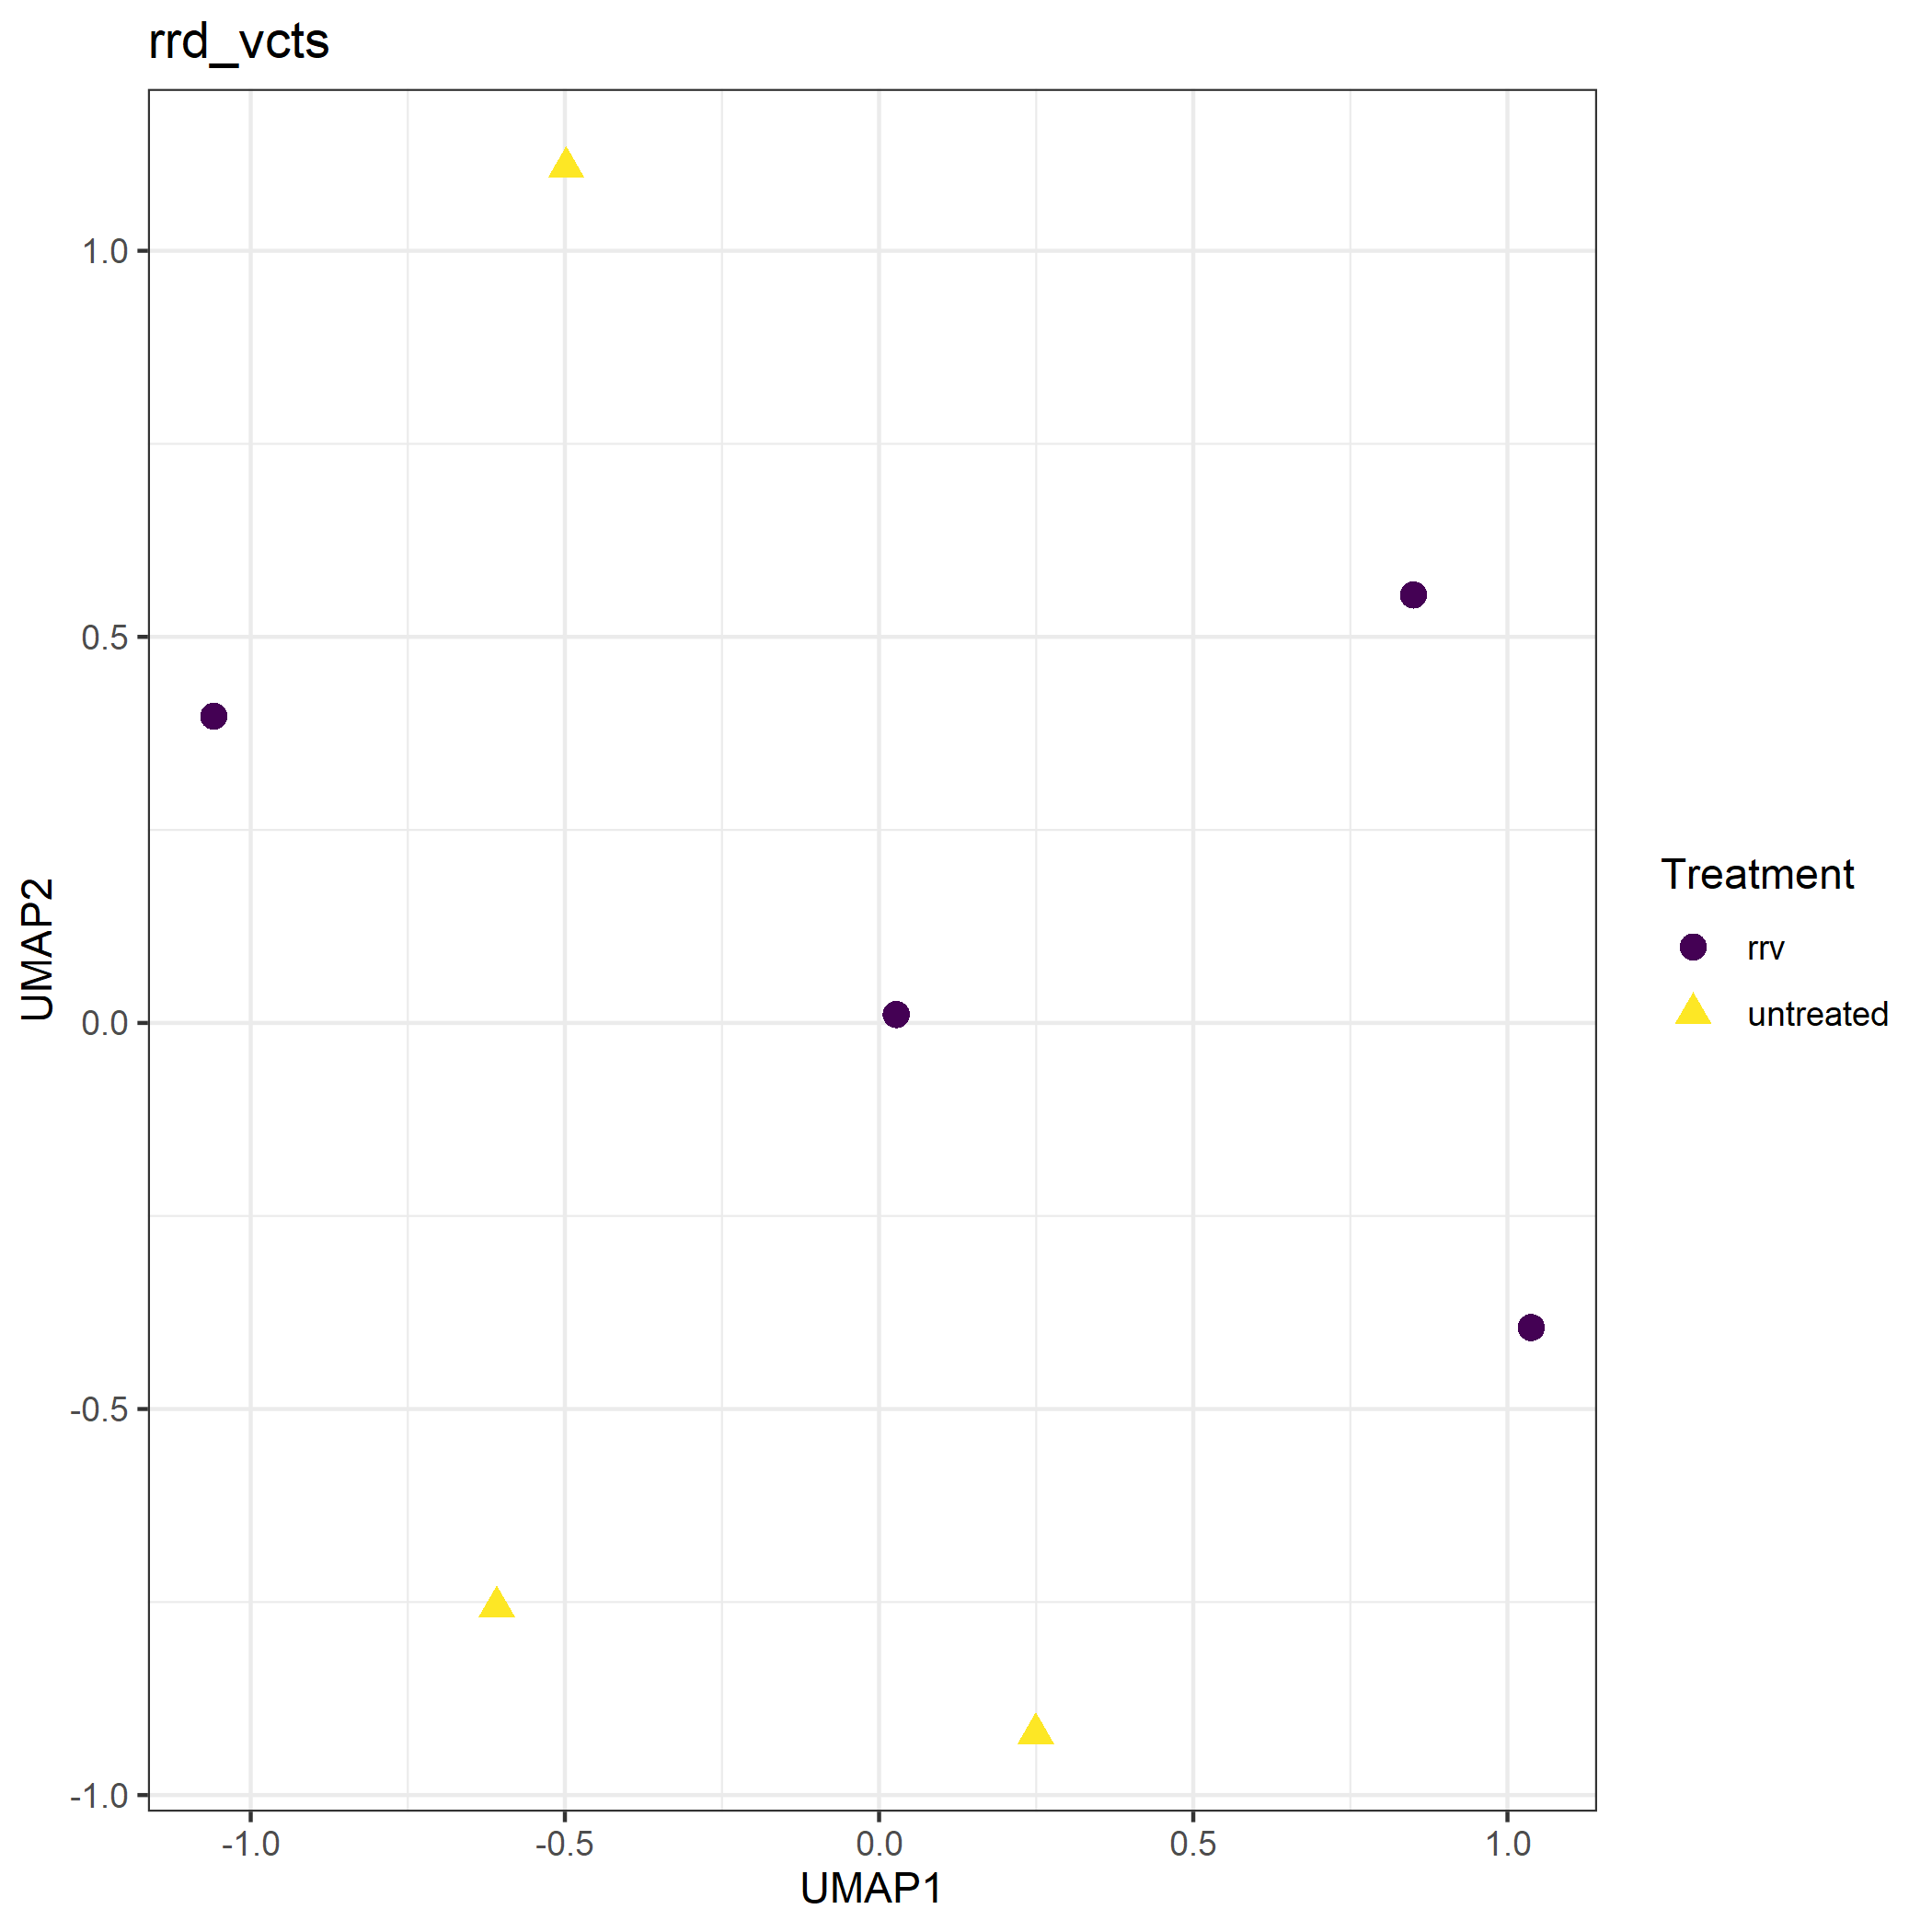
\includegraphics[width=1.1\linewidth]{figure/rrv_volatiles_umap_rrd_vcts} 

}

\caption[Uniform Manifold Approximation and Projection (UMAP) of VCT samples]{Uniform Manifold Approximation and Projection (UMAP) of VCT samples. Clusters represent similarities in chemical profile.}\label{fig:vcts-vocs-umap}
\end{figure}
\begin{figure}

{\centering 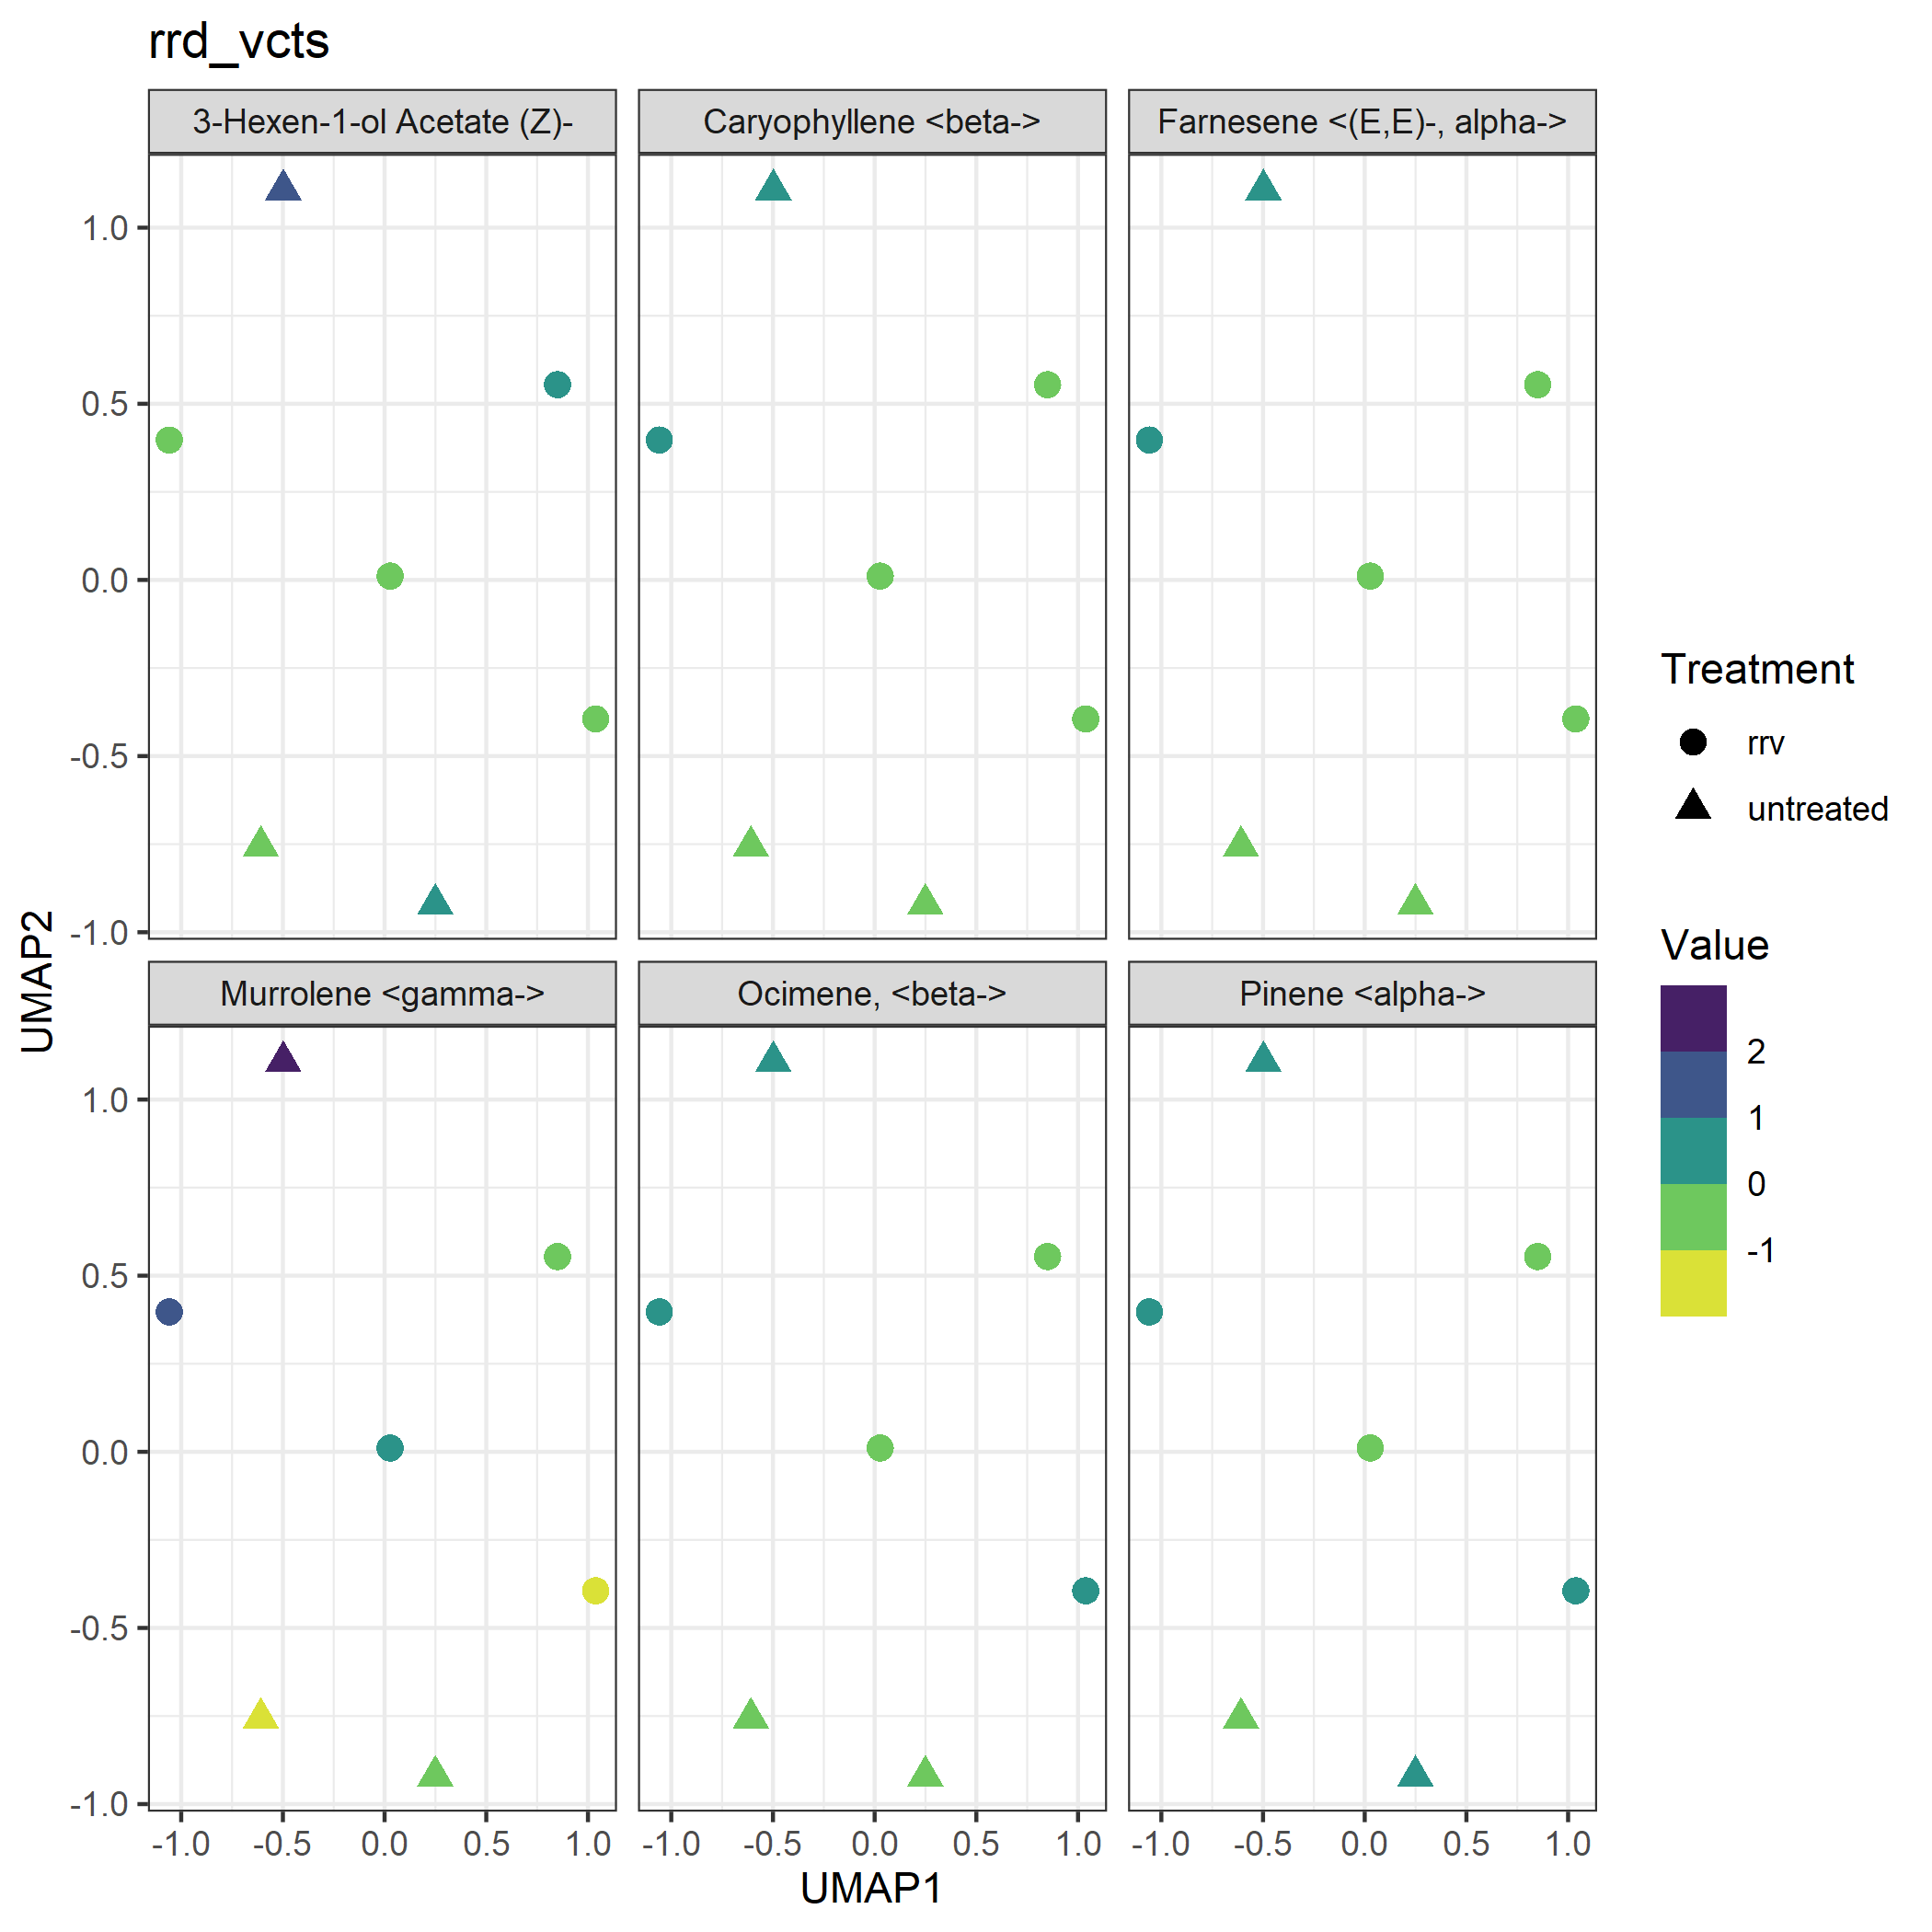
\includegraphics[width=1.1\linewidth]{figure/rrv_volatiles_umap_chems_rrd_vcts} 

}

\caption[UMAP of VCT method's ten largest contributions to volatile compositions. Clusters represent similarities in chemical profile.]{UMAP of VCT method's ten largest contributions to volatile compositions.}\label{fig:vcts-vocs-umap-chems}
\end{figure}
\FloatBarrier
\begin{figure}

{\centering 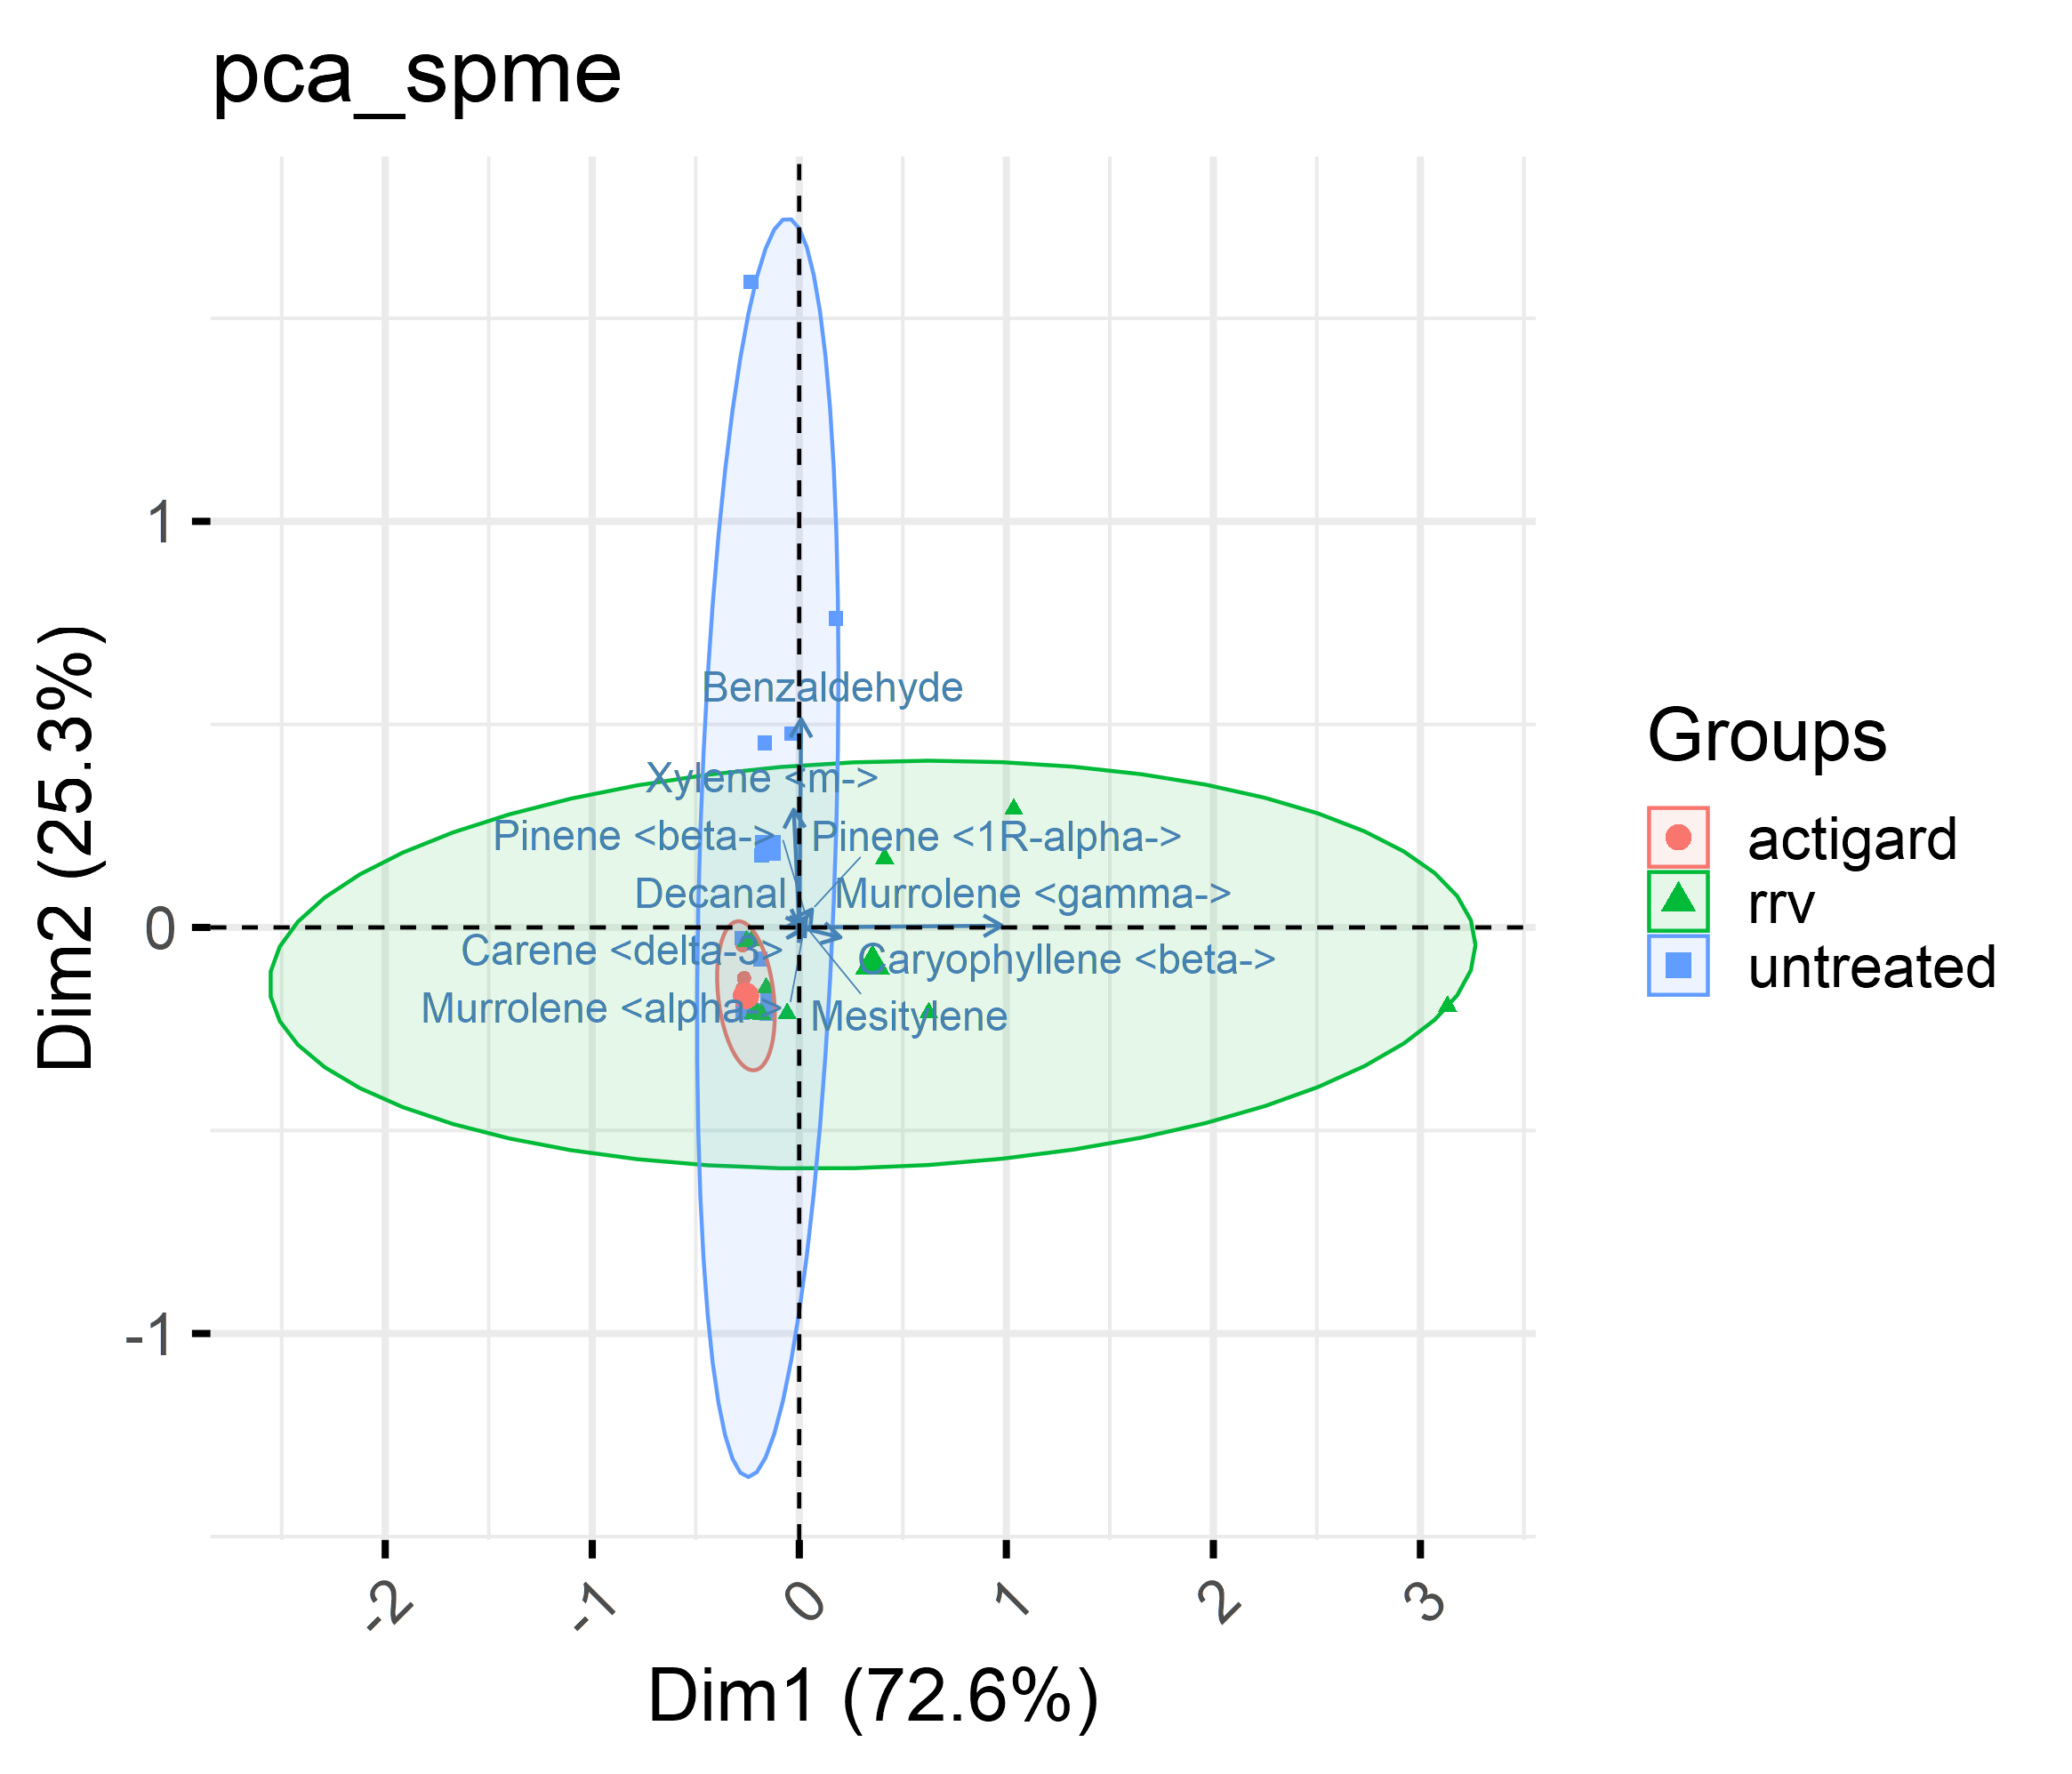
\includegraphics[width=1.1\linewidth]{figure/rrv_volatiles_pca_var_biplot_pca_spme} 

}

\caption[Principal component analysis (PCA) biplot of volatiles collected with Solid Phase Microextraction (SPME) methods.]{Principal component analysis (PCA) biplot of volatiles collected with Solid Phase Microextraction (SPME) methods. Ellipses represent 95\% confidence intervals. Clusters represent similarities in chemical profile.}\label{fig:spme-vocs-compares}
\end{figure}
\begin{figure}

{\centering 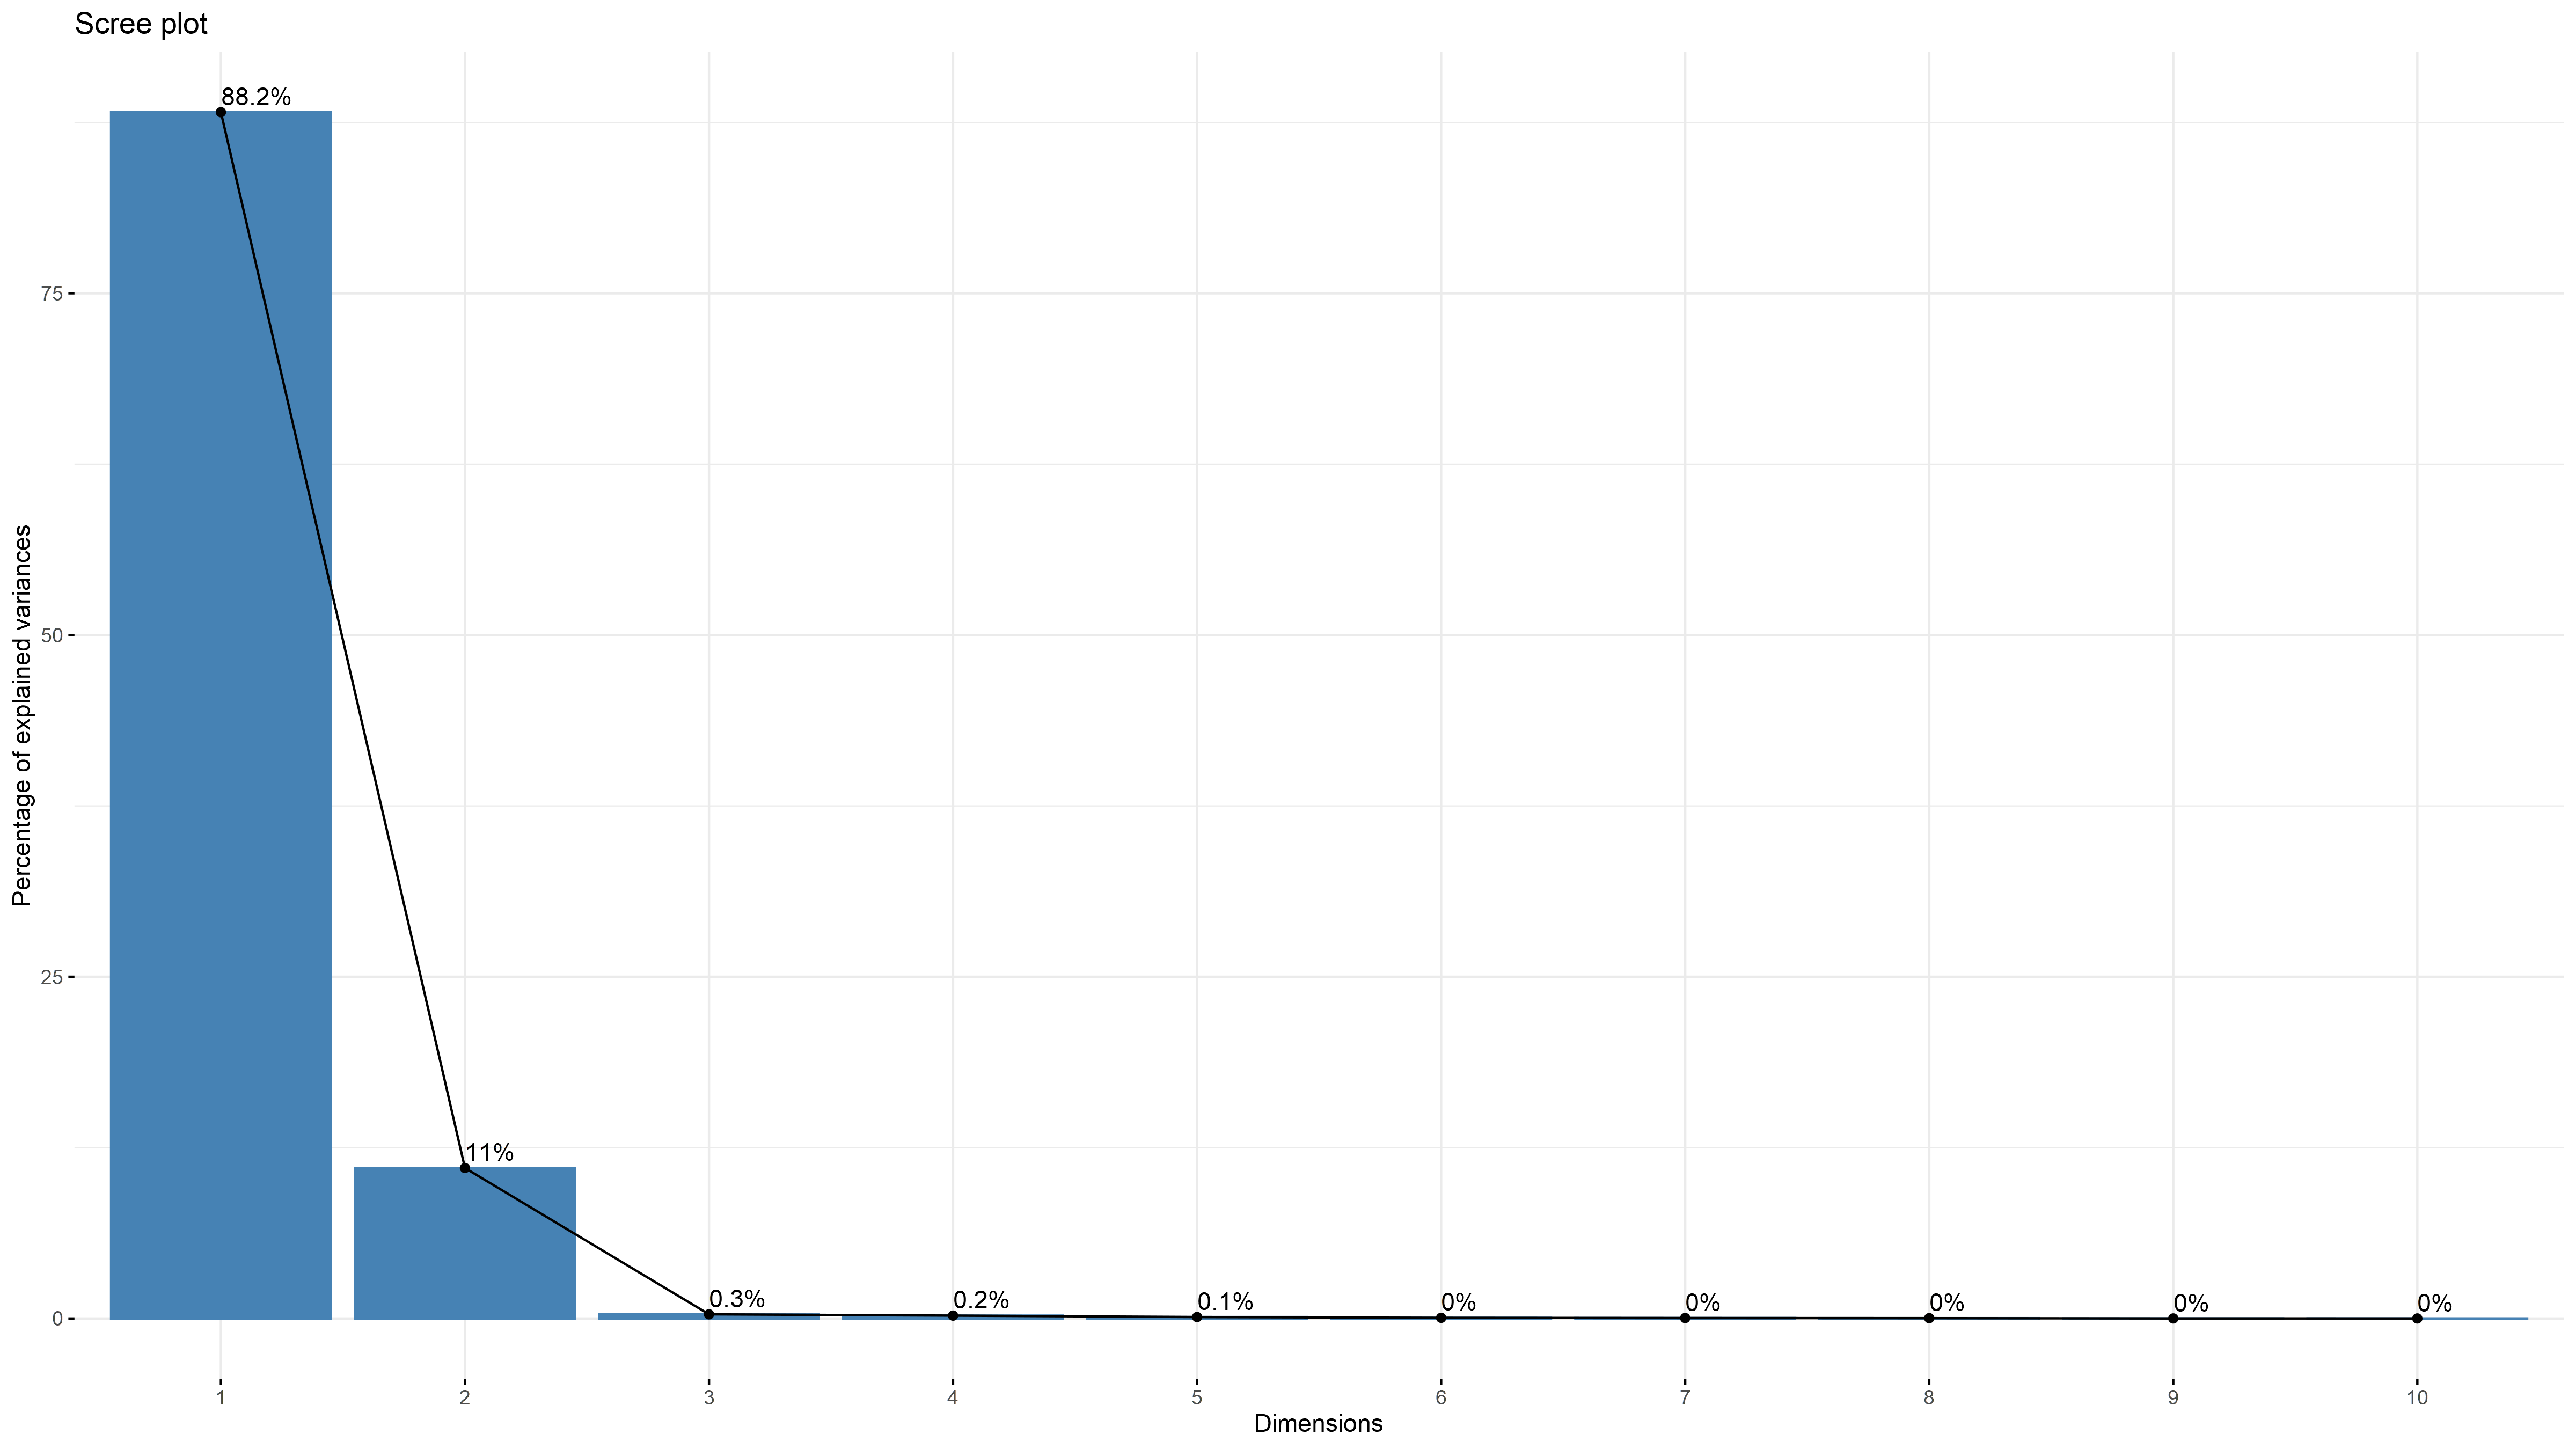
\includegraphics[width=1\linewidth]{figure/rrv_volatiles_screeplot_pca_spme} 

}

\caption[Scree plot of SPME principal components]{Scree plot of SPME principal components}\label{fig:spme-vocs-scree}
\end{figure}
\begin{figure}

{\centering 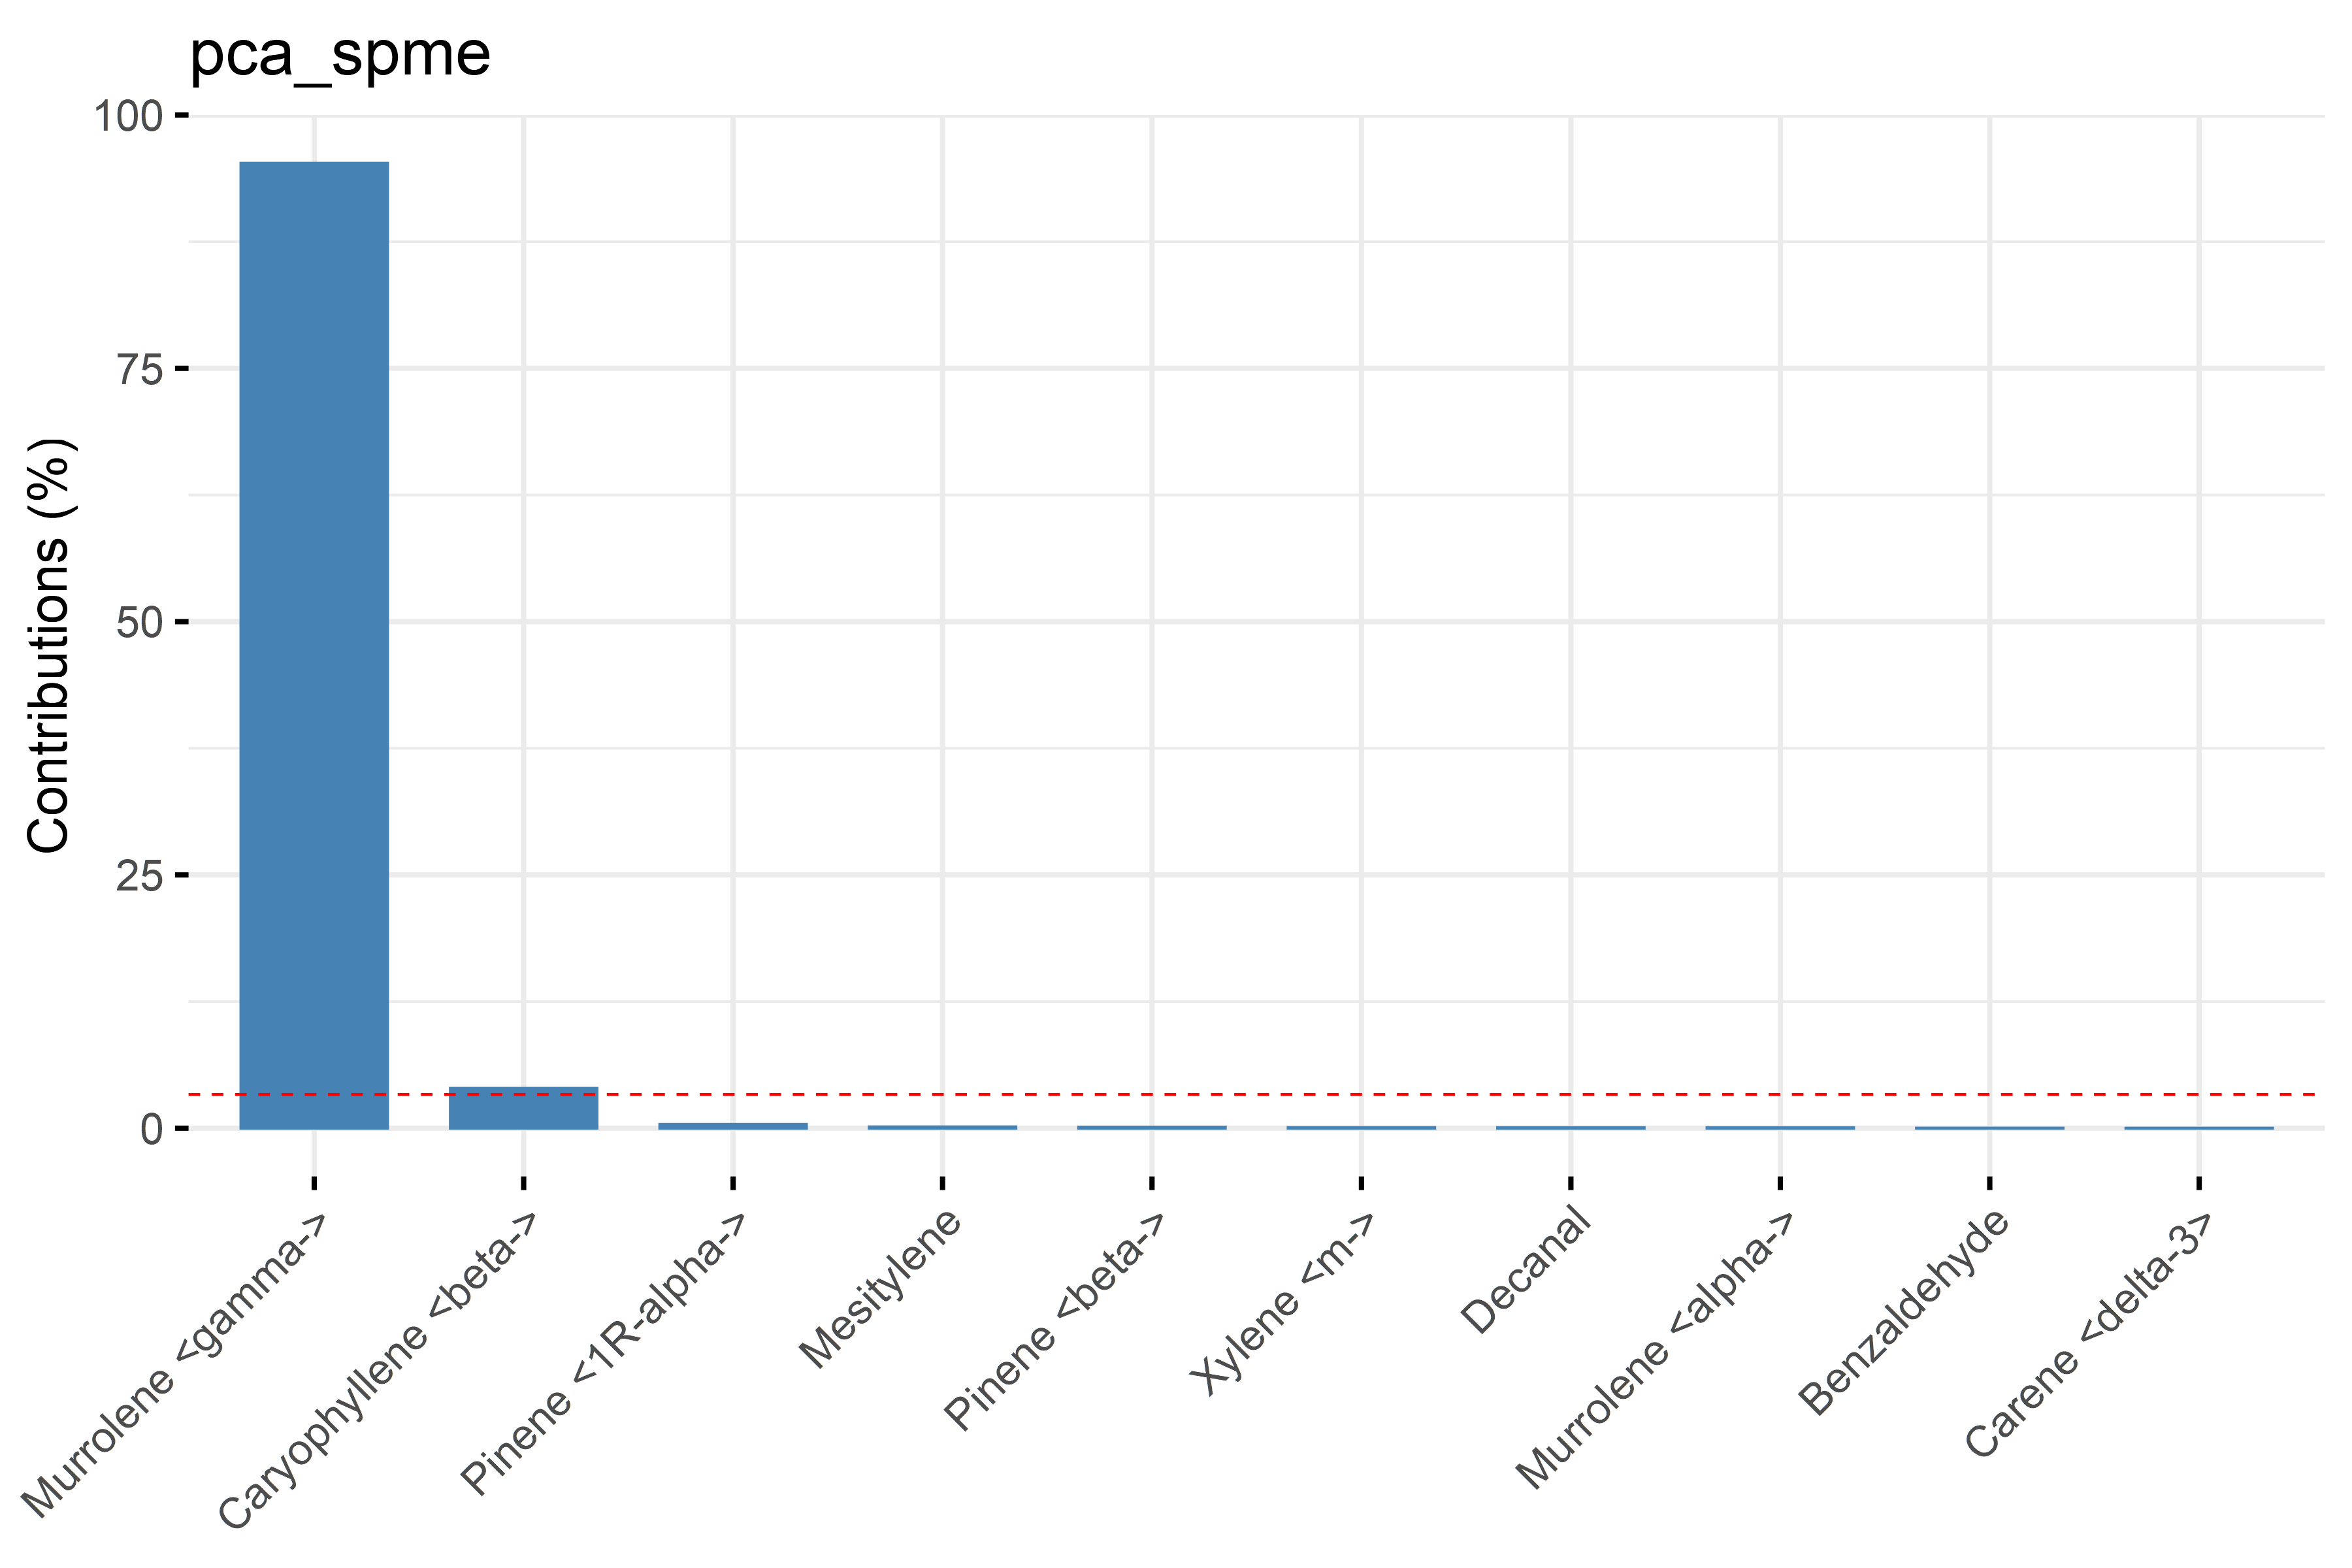
\includegraphics[width=1\linewidth]{figure/rrv_volatiles_var_pca_spme} 

}

\caption[Top ten contributing volatiles collected with SPME methods as determined by PCA.]{Top ten contributing volatiles collected with SPME methods as determined by PCA.}\label{fig:spme-vocs}
\end{figure}
\begin{table}

\caption{\label{tab:spme-contrib-table}Contribution table for PCA of headspace VOCs collected with SPME methods from Pink Double Knock Out® roses.}
\centering
\resizebox{\linewidth}{!}{
\begin{tabular}[t]{lrrr}
\toprule
Chemical & PCA1 & PCA2 & PCA3\\
\midrule
\cellcolor{gray!6}{Murrolene <gamma->} & \cellcolor{gray!6}{95.2415076} & \cellcolor{gray!6}{0.0053449} & \cellcolor{gray!6}{0.3441858}\\
Caryophyllene <beta-> & 3.9342124 & 0.1693947 & 10.4160243\\
\cellcolor{gray!6}{Pinene <1R-alpha->} & \cellcolor{gray!6}{0.3768098} & \cellcolor{gray!6}{0.5546385} & \cellcolor{gray!6}{2.2986334}\\
Mesitylene & 0.1335730 & 0.0002688 & 0.8001631\\
\cellcolor{gray!6}{Pinene <beta->} & \cellcolor{gray!6}{0.1116905} & \cellcolor{gray!6}{0.1813244} & \cellcolor{gray!6}{2.4829953}\\
\addlinespace
Xylene <m-> & 0.0713400 & 23.9618474 & 62.3968052\\
\cellcolor{gray!6}{Decanal} & \cellcolor{gray!6}{0.0581282} & \cellcolor{gray!6}{0.0397120} & \cellcolor{gray!6}{0.0663818}\\
Murrolene <alpha-> & 0.0574696 & 0.0000490 & 0.0049504\\
\cellcolor{gray!6}{Benzaldehyde} & \cellcolor{gray!6}{0.0078500} & \cellcolor{gray!6}{75.0832447} & \cellcolor{gray!6}{20.3483361}\\
Carene <delta-3> & 0.0024585 & 0.0008599 & 0.0266662\\
\addlinespace
\cellcolor{gray!6}{Bourbonene <beta->} & \cellcolor{gray!6}{0.0022327} & \cellcolor{gray!6}{0.0003698} & \cellcolor{gray!6}{0.2020302}\\
Copaene <alpha-> & 0.0007166 & 0.0003087 & 0.0899490\\
\cellcolor{gray!6}{Sulindac sulfide} & \cellcolor{gray!6}{0.0005104} & \cellcolor{gray!6}{0.0008275} & \cellcolor{gray!6}{0.0002247}\\
Nonanal & 0.0004008 & 0.0004141 & 0.1045067\\
\cellcolor{gray!6}{p-Cymene} & \cellcolor{gray!6}{0.0003913} & \cellcolor{gray!6}{0.0004774} & \cellcolor{gray!6}{0.0565775}\\
\addlinespace
Pinene <alpha-> & 0.0001973 & 0.0000038 & 0.0013929\\
\cellcolor{gray!6}{Squalene} & \cellcolor{gray!6}{0.0001843} & \cellcolor{gray!6}{0.0006171} & \cellcolor{gray!6}{0.3553188}\\
Cubebene <beta-> & 0.0001687 & 0.0000857 & 0.0017078\\
\cellcolor{gray!6}{Caryophyllene oxide} & \cellcolor{gray!6}{0.0000720} & \cellcolor{gray!6}{0.0000732} & \cellcolor{gray!6}{0.0017161}\\
Farnesene <(E,E)-, alpha-> & 0.0000449 & 0.0000114 & 0.0003219\\
\addlinespace
\cellcolor{gray!6}{Zonarene} & \cellcolor{gray!6}{0.0000171} & \cellcolor{gray!6}{0.0000013} & \cellcolor{gray!6}{0.0000096}\\
Phellandrene <beta-> & 0.0000120 & 0.0000197 & 0.0001646\\
\cellcolor{gray!6}{Pentadecane} & \cellcolor{gray!6}{0.0000089} & \cellcolor{gray!6}{0.0000522} & \cellcolor{gray!6}{0.0007362}\\
Dodecane & 0.0000034 & 0.0000497 & 0.0001903\\
\cellcolor{gray!6}{Hexadecane, 1-bromo-} & \cellcolor{gray!6}{0.0000002} & \cellcolor{gray!6}{0.0000026} & \cellcolor{gray!6}{0.0000055}\\
\addlinespace
Undecane & 0.0000000 & 0.0000001 & 0.0000016\\
\cellcolor{gray!6}{Benzaldehyde <para-ethyl->} & \cellcolor{gray!6}{0.0000000} & \cellcolor{gray!6}{0.0000001} & \cellcolor{gray!6}{0.0000001}\\
Limonene oxide, trans- & 0.0000000 & 0.0000000 & 0.0000030\\
\cellcolor{gray!6}{Terpineol <alpha->} & \cellcolor{gray!6}{0.0000000} & \cellcolor{gray!6}{0.0000000} & \cellcolor{gray!6}{0.0000013}\\
Bergamotene <alpha-, cis-> & 0.0000000 & 0.0000011 & 0.0000006\\
\bottomrule
\end{tabular}}
\end{table}
\begin{table}

\caption{\label{tab:spme-corr-table}Correlation table for PCA of headspace VOCs collected with SPME methods from Pink Double Knock Out® roses.}
\centering
\resizebox{\linewidth}{!}{
\begin{tabular}[t]{lrrr}
\toprule
Chemical & PCA1 & PCA2 & PCA3\\
\midrule
\cellcolor{gray!6}{Murrolene <gamma->} & \cellcolor{gray!6}{0.6348800} & \cellcolor{gray!6}{0.0028099} & \cellcolor{gray!6}{0.0053536}\\
Caryophyllene <beta-> & 0.1290350 & -0.0158185 & -0.0294511\\
\cellcolor{gray!6}{Pinene <1R-alpha->} & \cellcolor{gray!6}{0.0399337} & \cellcolor{gray!6}{0.0286233} & \cellcolor{gray!6}{-0.0138352}\\
Mesitylene & 0.0237759 & -0.0006301 & -0.0081628\\
\cellcolor{gray!6}{Pinene <beta->} & \cellcolor{gray!6}{0.0217414} & \cellcolor{gray!6}{0.0163660} & \cellcolor{gray!6}{-0.0143793}\\
\addlinespace
Decanal & 0.0156845 & 0.0076591 & -0.0023511\\
\cellcolor{gray!6}{Murrolene <alpha->} & \cellcolor{gray!6}{0.0155954} & \cellcolor{gray!6}{0.0002690} & \cellcolor{gray!6}{-0.0006421}\\
Benzaldehyde & 0.0057639 & 0.3330322 & 0.0411637\\
\cellcolor{gray!6}{Carene <delta-3>} & \cellcolor{gray!6}{0.0032256} & \cellcolor{gray!6}{-0.0011270} & \cellcolor{gray!6}{-0.0014902}\\
Bourbonene <beta-> & 0.0030739 & 0.0007391 & 0.0041016\\
\addlinespace
\cellcolor{gray!6}{Copaene <alpha->} & \cellcolor{gray!6}{0.0017414} & \cellcolor{gray!6}{0.0006753} & \cellcolor{gray!6}{0.0027368}\\
Pinene <alpha-> & 0.0009137 & 0.0000754 & -0.0003406\\
\cellcolor{gray!6}{Cubebene <beta->} & \cellcolor{gray!6}{0.0008449} & \cellcolor{gray!6}{-0.0003558} & \cellcolor{gray!6}{-0.0003771}\\
Caryophyllene oxide & 0.0005519 & -0.0003289 & -0.0003780\\
\cellcolor{gray!6}{Farnesene <(E,E)-, alpha->} & \cellcolor{gray!6}{0.0004358} & \cellcolor{gray!6}{-0.0001300} & \cellcolor{gray!6}{-0.0001637}\\
\addlinespace
Zonarene & 0.0002692 & -0.0000444 & -0.0000283\\
\cellcolor{gray!6}{Phellandrene <beta->} & \cellcolor{gray!6}{0.0002257} & \cellcolor{gray!6}{0.0001706} & \cellcolor{gray!6}{-0.0001171}\\
Undecane & 0.0000126 & -0.0000138 & -0.0000117\\
\cellcolor{gray!6}{Limonene oxide, trans-} & \cellcolor{gray!6}{0.0000065} & \cellcolor{gray!6}{-0.0000065} & \cellcolor{gray!6}{-0.0000158}\\
Bergamotene <alpha-, cis-> & -0.0000028 & 0.0000410 & 0.0000070\\
\addlinespace
\cellcolor{gray!6}{Terpineol <alpha->} & \cellcolor{gray!6}{-0.0000035} & \cellcolor{gray!6}{-0.0000009} & \cellcolor{gray!6}{-0.0000102}\\
Benzaldehyde <para-ethyl-> & -0.0000065 & -0.0000093 & -0.0000023\\
\cellcolor{gray!6}{Hexadecane, 1-bromo-} & \cellcolor{gray!6}{-0.0000287} & \cellcolor{gray!6}{-0.0000616} & \cellcolor{gray!6}{-0.0000215}\\
Dodecane & -0.0001204 & -0.0002710 & -0.0001259\\
\cellcolor{gray!6}{Pentadecane} & \cellcolor{gray!6}{-0.0001940} & \cellcolor{gray!6}{0.0002776} & \cellcolor{gray!6}{0.0002476}\\
\addlinespace
Squalene & -0.0008831 & -0.0009547 & -0.0054395\\
\cellcolor{gray!6}{p-Cymene} & \cellcolor{gray!6}{-0.0012868} & \cellcolor{gray!6}{0.0008397} & \cellcolor{gray!6}{0.0021706}\\
Nonanal & -0.0013024 & -0.0007821 & -0.0029500\\
\cellcolor{gray!6}{Sulindac sulfide} & \cellcolor{gray!6}{-0.0014697} & \cellcolor{gray!6}{0.0011056} & \cellcolor{gray!6}{-0.0001368}\\
Xylene <m-> & -0.0173758 & 0.1881373 & -0.0720828\\
\bottomrule
\end{tabular}}
\end{table}
\begin{figure}

{\centering 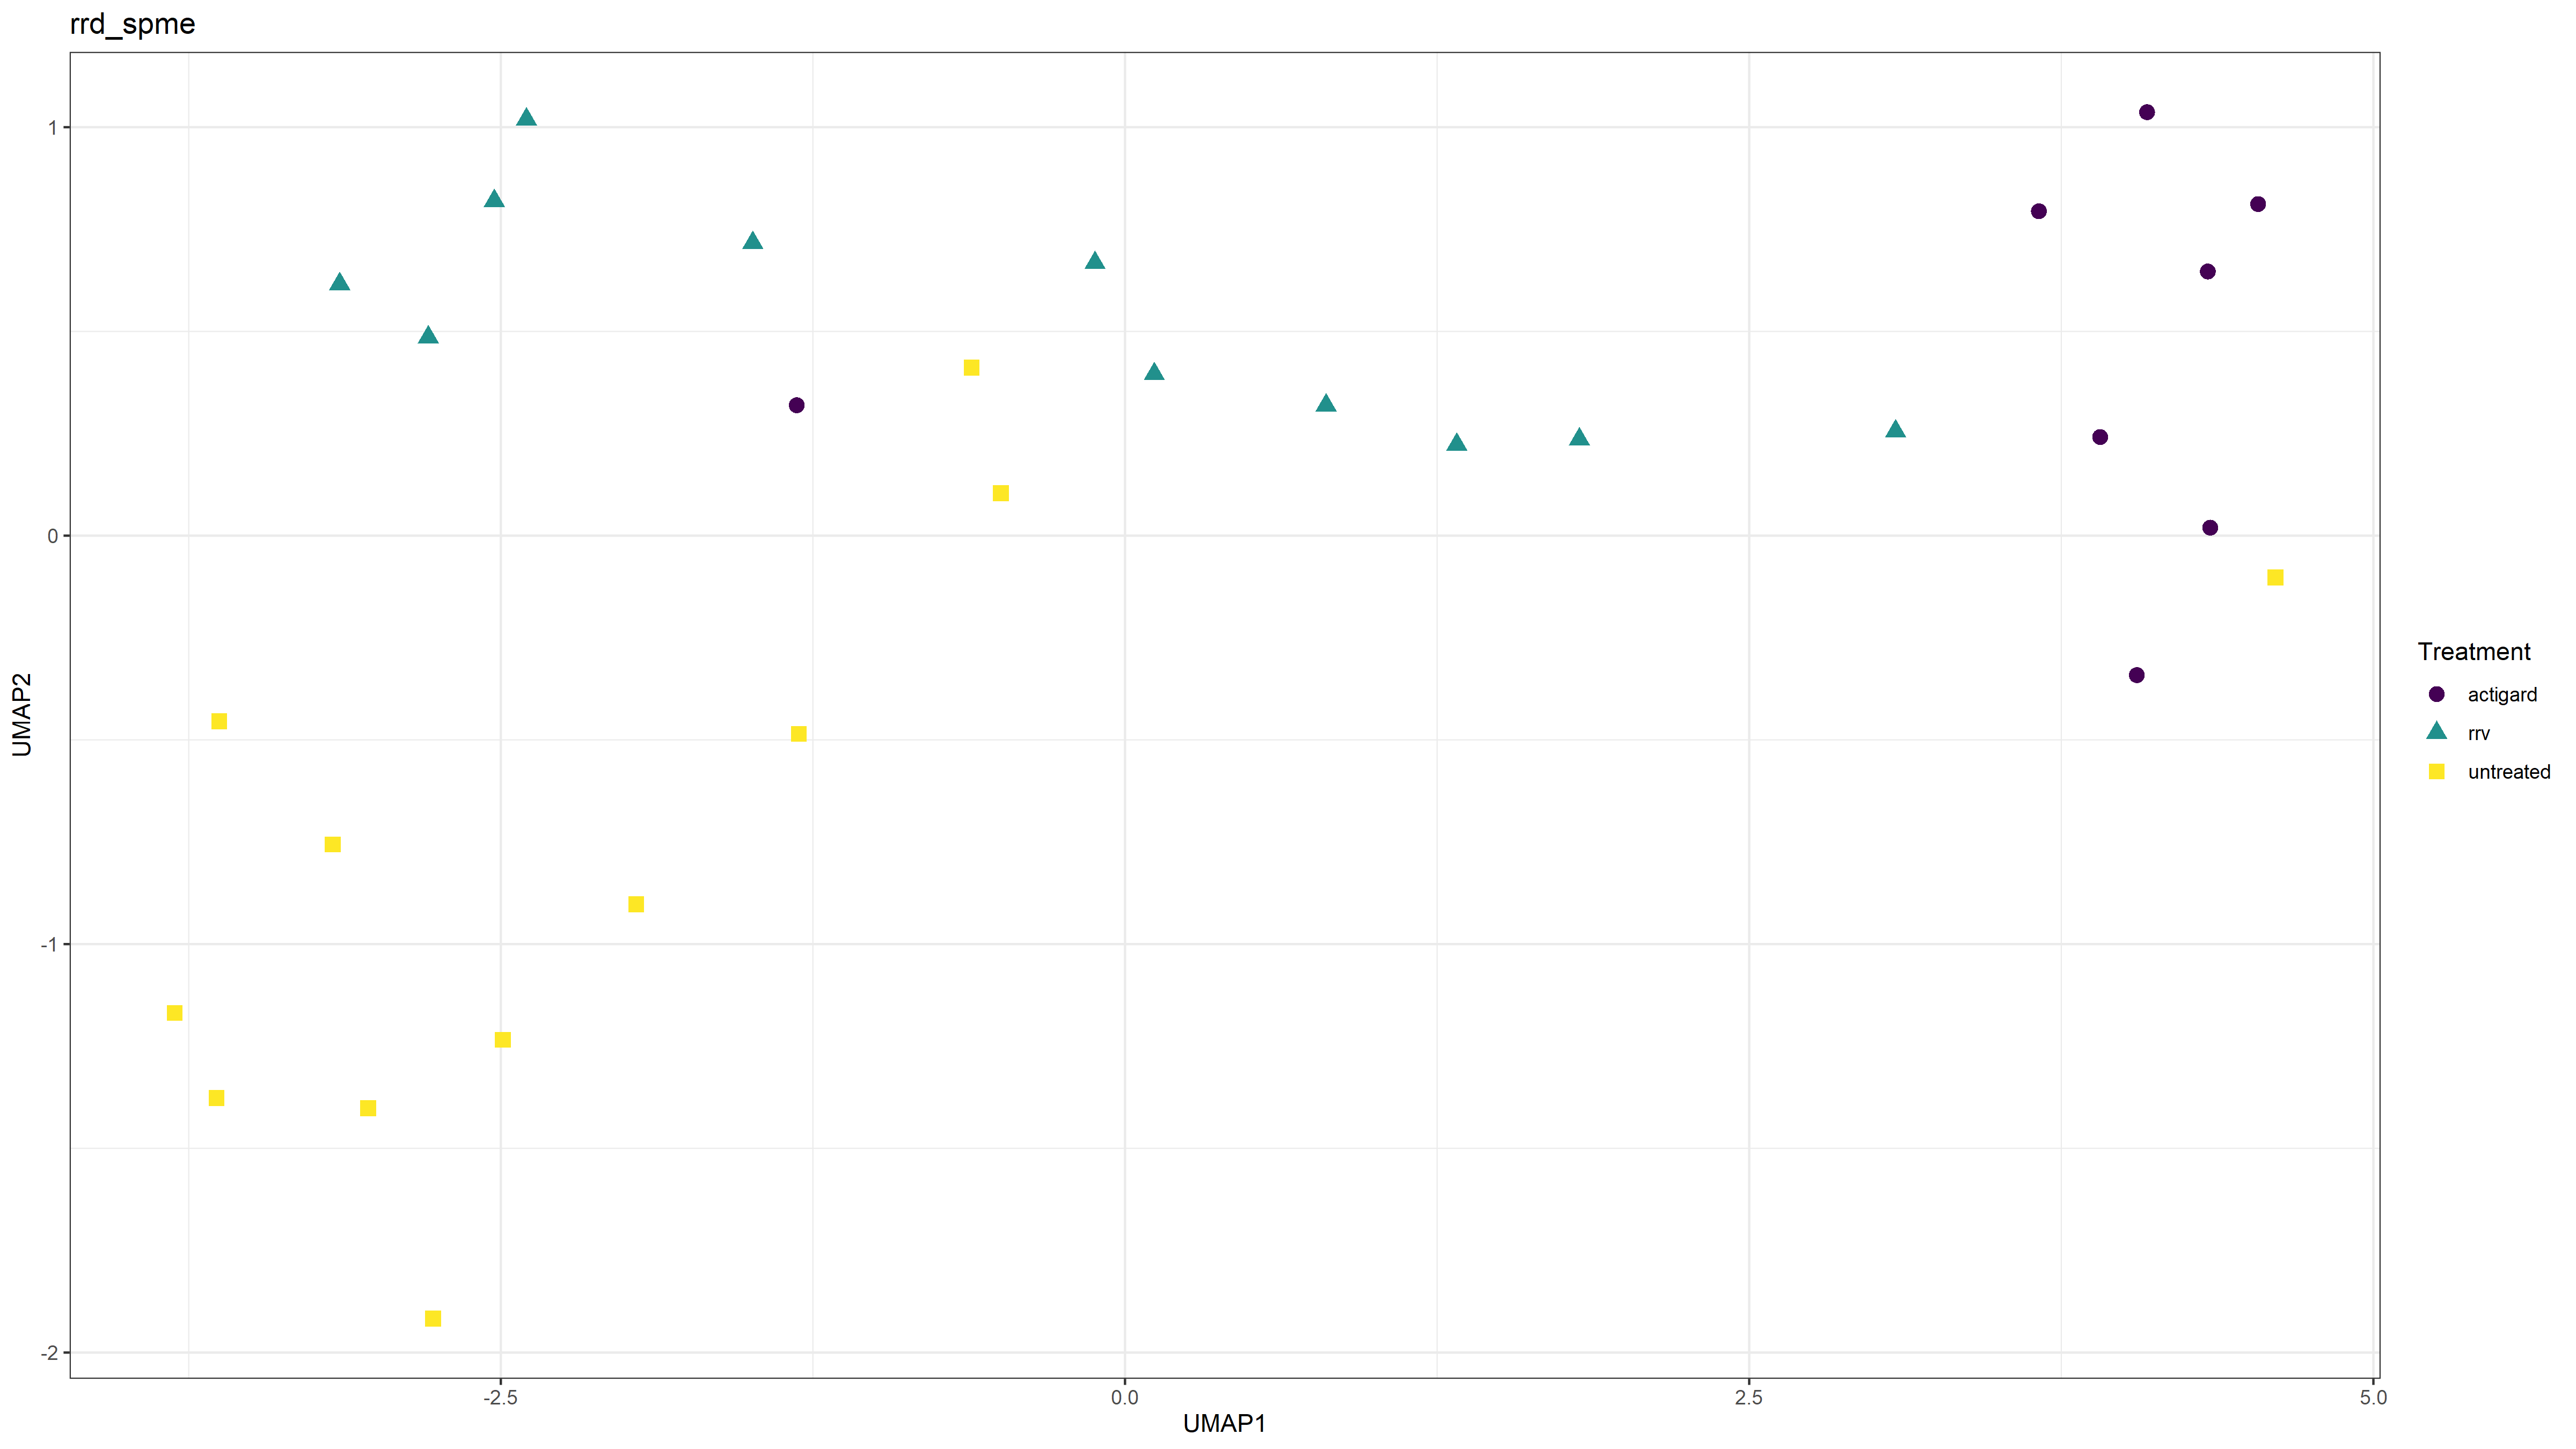
\includegraphics[width=1.1\linewidth]{figure/rrv_volatiles_umap_rrd_spme} 

}

\caption[UMAP of SPME method volatiles]{UMAP of SPME method volatiles. Clusters represent similarities in chemical profile.}\label{fig:spme-vocs-umap}
\end{figure}
\begin{figure}

{\centering 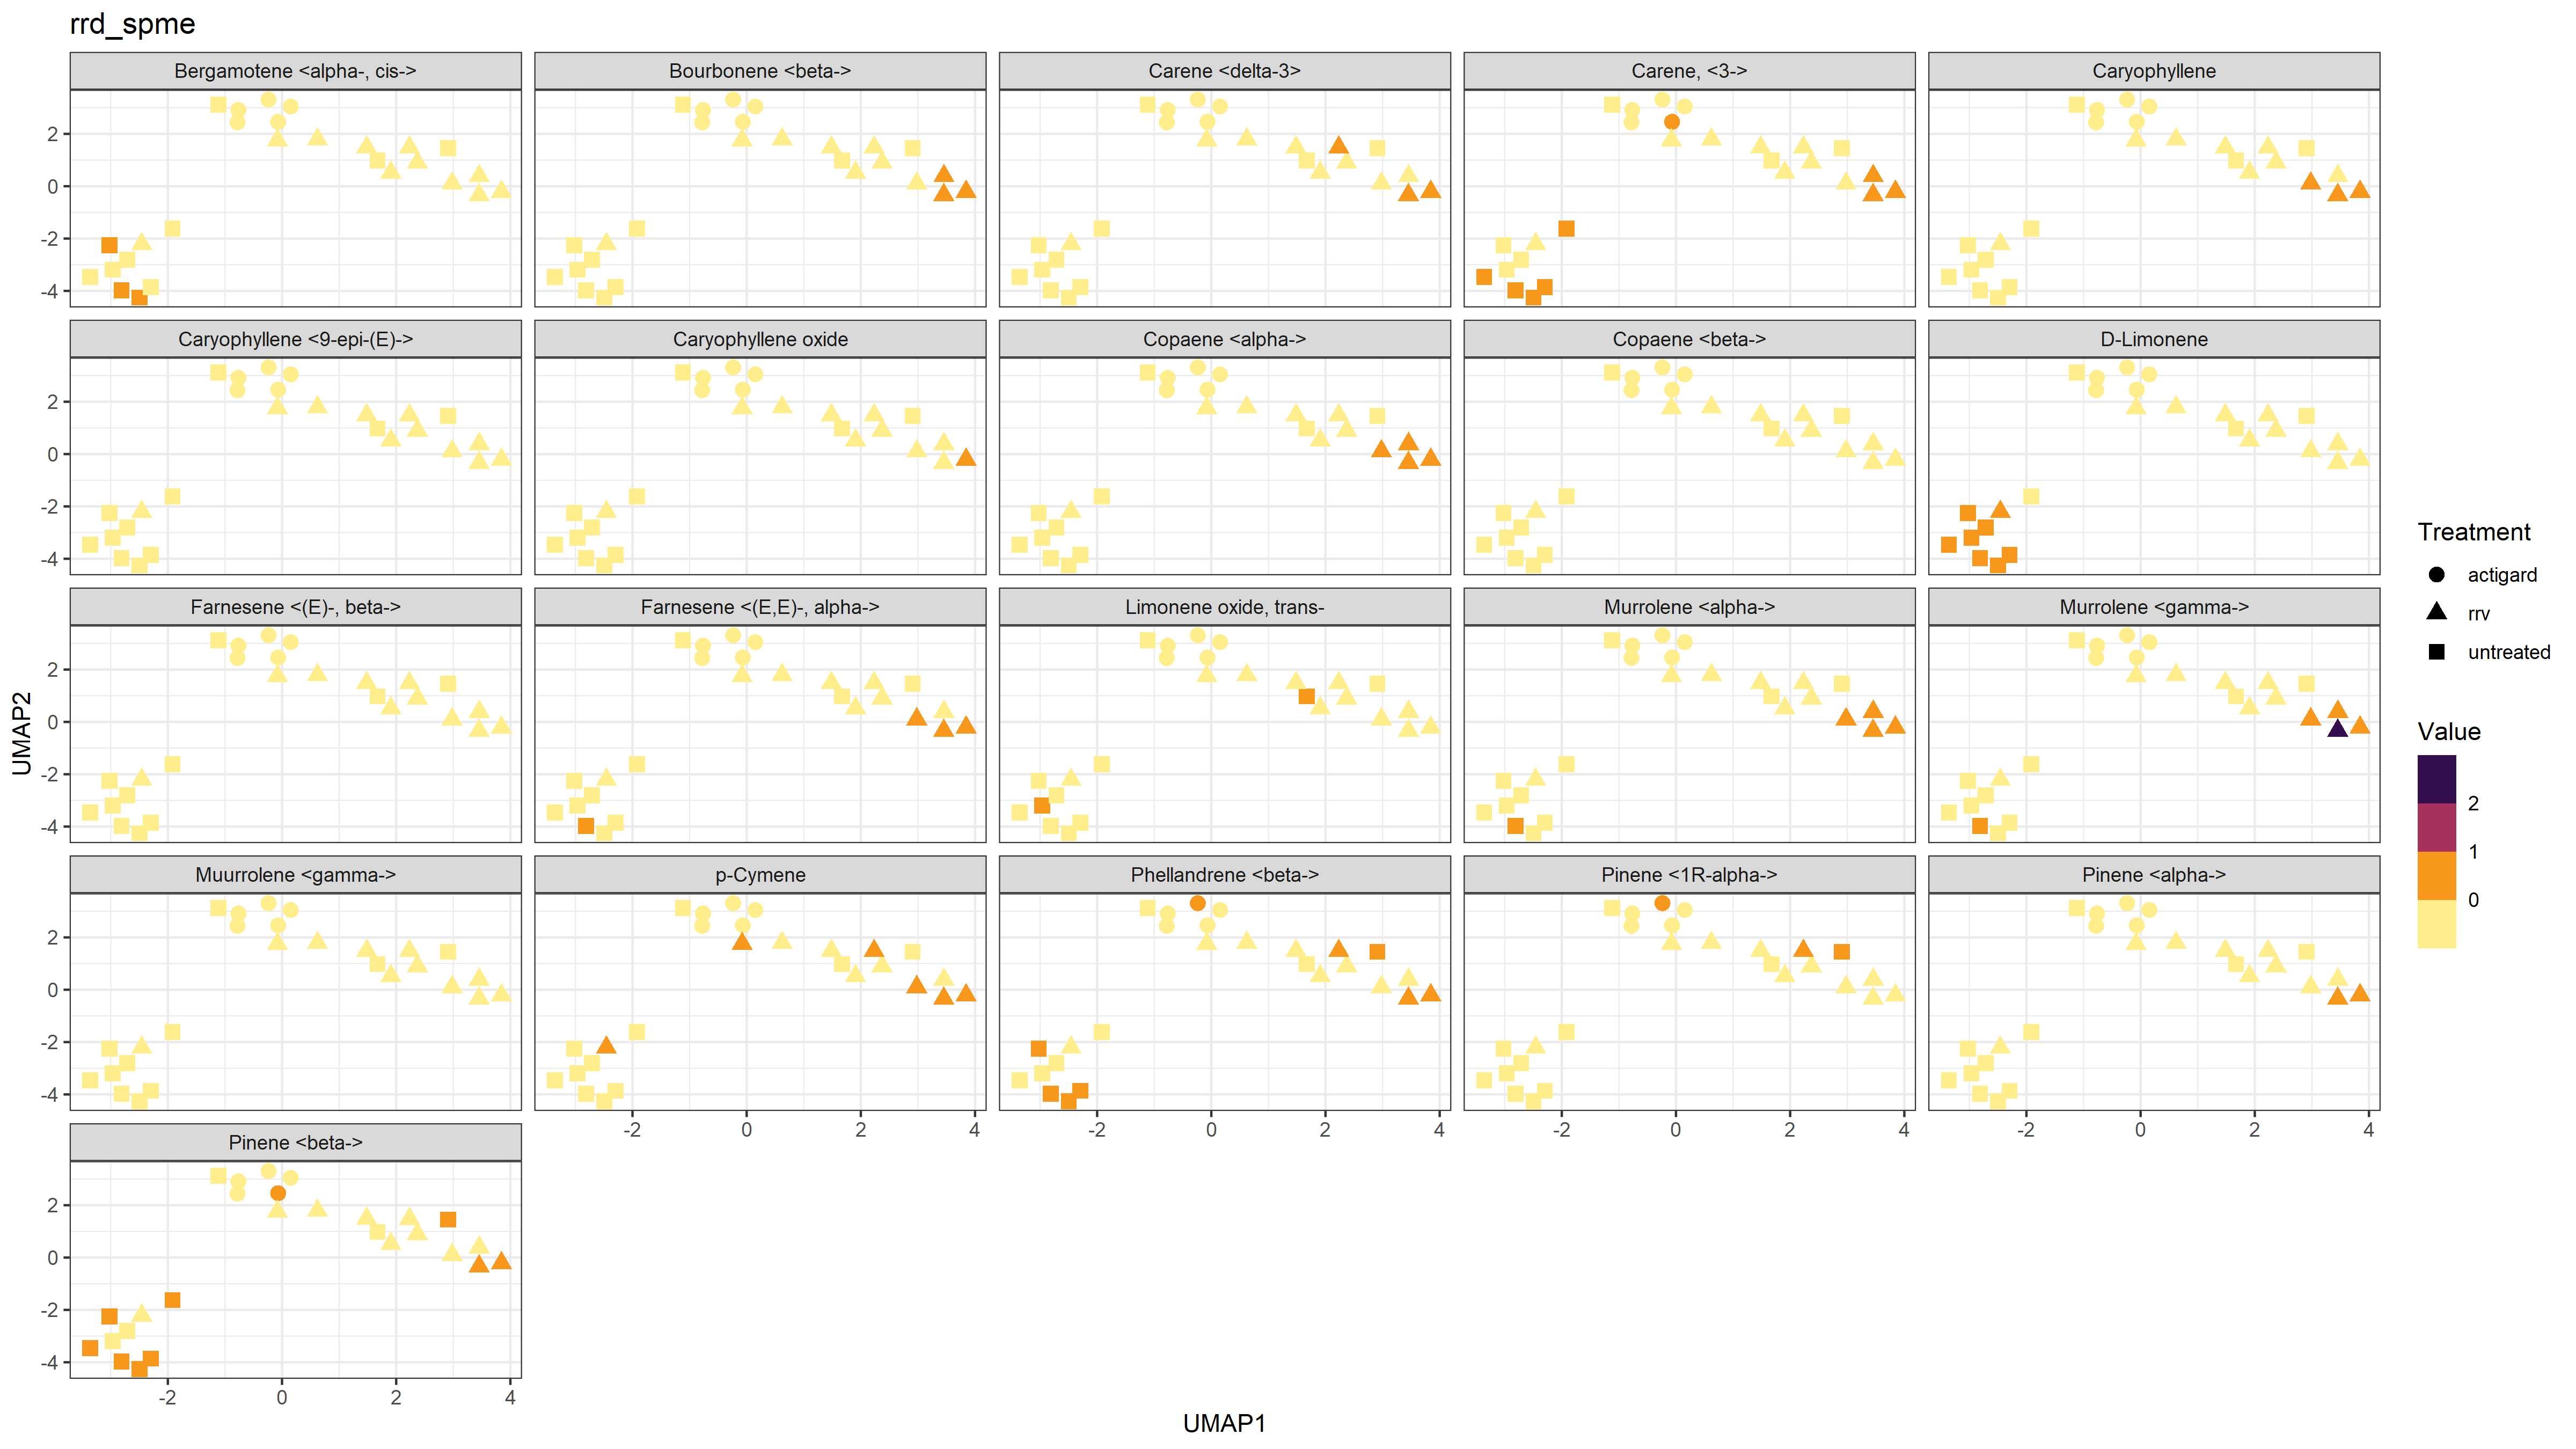
\includegraphics[width=1.1\linewidth]{figure/rrv_volatiles_umap_chems_rrd_spme} 

}

\caption[UMAP of SPME method's ten largest contributions to volatile compositions]{UMAP of SPME method's ten largest contributions to volatile compositions. Clusters represent similarities in chemical profile.}\label{fig:spme-vocs-umap-chems}
\end{figure}
\hypertarget{discussion-1}{%
\section{Discussion}\label{discussion-1}}

Plants play a large role in the lives of phytoseiid mites (\protect\hyperlink{ref-Cortesero2000}{Cortesero et al. 2000}, \protect\hyperlink{ref-Schmidt2013}{Schmidt 2013}): for example the trichome density of plants affects their dispersal (\protect\hyperlink{ref-Loughner2010}{Loughner et al. 2010a}, \protect\hyperlink{ref-Loughner2010a}{2010b}, \protect\hyperlink{ref-Buitenhuis2013}{Buitenhuis et al. 2013}, \protect\hyperlink{ref-Lopez2016}{Lopez et al. 2016}), oviposition, (\protect\hyperlink{ref-ODowd1991}{O'Dowd and Willson 1991}, \protect\hyperlink{ref-Walter1992}{Walter 1992}, \protect\hyperlink{ref-Walter1996}{1996}, \protect\hyperlink{ref-Grostal1994}{Grostal and O'Dowd 1994}, \protect\hyperlink{ref-Agrawal1997}{Agrawal and Karban 1997}), performance as predators (\protect\hyperlink{ref-Cedola2001}{Cédola et al. 2001}, \protect\hyperlink{ref-Seelmann2007}{Seelmann et al. 2007}, \protect\hyperlink{ref-Buitenhuis2013}{Buitenhuis et al. 2013}) and their ability to avoid predation (\protect\hyperlink{ref-Faraji2002}{Faraji et al. 2002}). Therefore, it is not unusual to see a preference towards plant VOCs, but it is interesting to note their attraction to an infected rose (\emph{\ref{fig:aswir-rrd}}). Future tests should try varying the concentrations of these chemicals, and testing the other chemicals detected from the volatile extractions. Olfactometers are considered a useful way to determine predatory mite attraction to different plant volatiles (\protect\hyperlink{ref-Janssen1990}{Janssen et al. 1990}). It is interesting to note that VCT methods found that levels of MeSA were lower for infected plants; SPME methods did not recover MeSA. It may be that SPME fibers were not exposed to VOCs long enough on infected roses to reach equilibrium, or MeSA is very low in severely infected plants. It is also peculiar to see that MeSA levels were not recovered from ASM-treated plants (\emph{\ref{tab:spme-contrib-table}, \ref{tab:spme-corr-table}}). ASM induces SAR, again possibly that SPME fibers may not be adsorbing MeSA in our assays for some reason. Furthermore, ASM-treated plants had lower volatile activity overall, compared to other roses, which may explain the clustering we see in our figures (\emph{\ref{fig:spme-vocs-compares}}, \emph{\ref{fig:vcts-vocs-compares}}). Unfortunately, these data are not truly comparable due to the inherent differences in the collecting methods used. Another possibility is that the time of sampling affected the outcome, as SPME is affected by temperature and plant volatiles are regulated by both time of day and UV exposure (\protect\hyperlink{ref-Griebel2008}{Griebel and Zeier 2008}, \protect\hyperlink{ref-EscobarBravo2019}{Escobar-Bravo et al. 2019}). Double Knock Out® roses are known to have less fragrance than other rose cultivars, suggesting lower levels of volatile emissions from petals (\protect\hyperlink{ref-Bergougnoux2007}{Bergougnoux et al. 2007}), which may have affected the quantities of the VOCs collected. Another issue comes from the field aspects of the study, with multiple herbivores present on the roses in the landscape which could activate different plant defenses. For example, \emph{T. urticae} are known to activate both SA and JA signalling pathways during feeding (\protect\hyperlink{ref-Ozawa2000}{Ozawa et al. 2000}), which may be interfering with volatiles which would normally be introduced by an infestation of just \emph{P. fructiphilus} Herbivore induced plant volatiles often last only for a few days after induction (\protect\hyperlink{ref-Choh2007}{Choh and Takabayashi 2007}), but ASM-treated plants were sampled at the end of a 12-week application period, so these plants may have downregulated their production of MeSA by the time of sampling. This is an unfortunate side effect of sampling in the field at a remote site rather than in the lab. The SPME method is limited to short extractions, partially due to overheating of the inflator pumps. It is harder to have high confidence about results without VCT validation, due to the many variables and possible confounding effects such as plant age, measurement error, sample contamination, temperature, etc.. Sampling recently SAR-induced plants with VCT methods would give a good point of reference to resolve this discrepancy. If MeSA levels are truly low on infected roses, it may suggest that MeSA was not the primary chemical involved with attracting \emph{A. swirskii} to roses. The most common VOCs extracted from roses were terpenes. \textgamma-Murrolene and \textbeta-Caryophyllene were the largest contributors to the VOC composition from the roses collected, so it would be worth testing these chemicals with \emph{A. swirskii} to see if these chemicals play a role in \emph{A. swirskii} attraction to infected roses. Mites were not more attracted to Limonene than filtered air in our preliminary trials, but there were differences in time to choice (\emph{\ref{fig:aswir-mesa-lim-times}}) and a significant difference between making a choice vs.~no choice (\emph{\ref{fig:aswir-mesa-lim}}). On the contrary to the Limonene results, \emph{A. swirskii} appeared to have random behaviors between choices and no-choice, and did not vary in their time to choice (\emph{\ref{fig:aswir-mesa-lim}}, \emph{\ref{fig:aswir-mesa-lim-times}}). We predict that reducing the concentrations of these synthetic VOCs may produce different responses, more experiments are warranted. In conclusion, we have found preliminary data about volatile changes in infected roses and SAR-induced roses, and their putative relationships with \emph{A. swirskii}.

\hypertarget{management-of-phyllocoptes-fructiphiulus-with-systemic-acquired-resistance}{%
\chapter{\texorpdfstring{MANAGEMENT OF \emph{Phyllocoptes fructiphiulus} WITH SYSTEMIC ACQUIRED RESISTANCE}{MANAGEMENT OF Phyllocoptes fructiphiulus WITH SYSTEMIC ACQUIRED RESISTANCE}}\label{management-of-phyllocoptes-fructiphiulus-with-systemic-acquired-resistance}}

\hypertarget{introduction-phyllocoptes-fructiphiulus---small-mites-creating-big-problems}{%
\section{\texorpdfstring{Introduction: \emph{Phyllocoptes fructiphiulus} - Small Mites Creating Big Problems}{Introduction: Phyllocoptes fructiphiulus - Small Mites Creating Big Problems}}\label{introduction-phyllocoptes-fructiphiulus---small-mites-creating-big-problems}}

\emph{Phyllocoptes fructiphilus} Keifer (Trombidiformes: Eriophyidae) is a microscopic plant-feeding arachnid known as an eriophyid mite. \emph{P. fructiphilus} is host specific, only feeding on plants in the genus \emph{Rosa}, and normally cause little damage by itself. Unfortunately, \emph{P. fructiphilus} has become infamous due to Rose Rosette Virus (RRV), a pathogen which the mite transmits while feeding. RRV infection creates the following symptoms: witches' brooms/rosetting, deformed flowers, increased prickle density, elongated shoots, reddened leaves and stems, and increased die-back which ultimately kills the rose host (\protect\hyperlink{ref-Allington1968}{Allington et al. 1968}, \protect\hyperlink{ref-Tzanetakis2006}{Tzanetakis et al. 2006}, \protect\hyperlink{ref-Laney2011}{Laney et al. 2011}). This disease is known as Rose Rosette Disease (RRD) and is widely considered the most serious disease of roses in the US. RRD and the mite have invaded the southeastern US as they followed the range expansion of the non-native \emph{Rosa multiflora} (Thunb) towards the coast (\protect\hyperlink{ref-Amrine1996}{Amrine Jr 1996}, \protect\hyperlink{ref-Amrine2002}{2002}, \protect\hyperlink{ref-Otero-Colina2018}{Otero-Colina et al. 2018}). RRD afflicts a passionate group from different sectors of the US rose industry, including homeowners, commercial landscapers, nurseries, conservationists, and rosarians, all of whom stand to lose millions of dollars and many established roses plantings in the coming years Rwahnih et al. (\protect\hyperlink{ref-Rwahnih2019}{2019}). Florida, as the nation's largest producer of roses, has a special interest developing methods to better control \emph{P. fructiphilus} and RRD. There is a critical need to improve management of \emph{P. fructiphilus} and RRD. Unfortunately, few commercially available roses have resistance to RRD (\protect\hyperlink{ref-Bello2017}{Di Bello et al. 2017}, \protect\hyperlink{ref-Byrne2018}{Byrne et al. 2018}). Presently, growers are recommended to manage the \emph{P. fructiphilus} by removing plants and spraying pesticides (\protect\hyperlink{ref-Hong2012}{Hong et al. 2012}, \protect\hyperlink{ref-Olson2017}{Olson et al. 2017}, \protect\hyperlink{ref-UGA2018}{{``Control - rose rosette''} 2018}). However, pesticides have come under increased public scrutiny due to concerns about health, the environment, pest resistance, and harm to pollinators Vanbergen and Insect Pollinators Initiative (\protect\hyperlink{ref-Vanbergen2013}{2013}). Increased pesticide applications also decrease grower profits and reduce competitiveness with foreign markets. The lack of alternative or complementary management options exacerbates this issue: rose growers need more options for \emph{P. fructiphilus} control, especially methods which can be integrated into existing management programs. In 2013, nursery workers in Quincy, Gadsden County, Florida, USA, detected unusual red growths, deformed stems and extra thorniness on 15 knockout roses which had been imported from out of state. Eight symptomatic plants were tested by our Plant Diagnostic Clinic at the University of Florida's North Florida Research and Education Center in Quincy, FL, and found to be positive for RRD, but the \emph{P. fructiphilus} mites were not detected at that time (\protect\hyperlink{ref-Babu2014}{Babu et al. 2014}). On February 14, 2019, populations of \emph{P. fructiphilius} were encountered on roses in Tallahassee, Leon County, Florida (\protect\hyperlink{ref-Fife2020}{Fife et al. 2020}). The existence of \emph{P. fructiphilus} in northern Florida increases the the possibility of introducing RRD from areas where the disease had become established, including the neighboring states of Georgia and Alabama (\protect\hyperlink{ref-Solo2018}{Solo 2018}, \protect\hyperlink{ref-Solo2020}{Solo et al. 2020}).

\hypertarget{integrating-pest-management-what-are-the-effects-of-systemic-acquired-resistance-on-amblyseius-swirskii-and-phyllocoptes-fructiphilus}{%
\subsection{\texorpdfstring{Integrating pest management: what are the effects of systemic acquired resistance on \emph{Amblyseius swirskii} and \emph{Phyllocoptes fructiphilus}?}{Integrating pest management: what are the effects of systemic acquired resistance on Amblyseius swirskii and Phyllocoptes fructiphilus?}}\label{integrating-pest-management-what-are-the-effects-of-systemic-acquired-resistance-on-amblyseius-swirskii-and-phyllocoptes-fructiphilus}}

Integrated Pest Management (IPM) is the combination of science-informed best practices designed to keep the cost of pest control below the value of the crop damages which would occur without intervention (i.e.~economic injury level) (\protect\hyperlink{ref-Stern1959}{Stern et al. 1959}, \protect\hyperlink{ref-Flint1981}{Flint and Bosch 1981}, \protect\hyperlink{ref-USDA2018}{USDA-ARS 2018}). In practice, IPM is informed by an understanding of the pest's biology and the judicious use of chemical controls, natural predators (biological controls), plant breeding, plant immune systems and physical (cultural) controls as needed to control pests as efficiently as possible (\protect\hyperlink{ref-Bradley2018}{Bradley and Moore 2018}). Our lab has been investigating the potential of inducing systemic acquired resistance (SAR) to provide protect from mite herbivory as well as pathogen damage (\protect\hyperlink{ref-Cole1999}{Cole 1999}, \protect\hyperlink{ref-Anfoka2000}{Anfoka 2000}, \protect\hyperlink{ref-Babu2021}{Babu et al. 2021}, \protect\hyperlink{ref-Doungous2021}{Doungous et al. 2021}). Induction of SAR may be able to disrupt the establishment of eriophyoid mites (\protect\hyperlink{ref-Bronner1991}{Bronner et al. 1991a}, \protect\hyperlink{ref-Bronner1991a}{1991b}, \protect\hyperlink{ref-Westphal1991}{Westphal et al. 1991}). Infested and SAR-induced plants produce \textbeta-1,3-glucanase and chitinases, which were hypothesized to contribute to plant defenses against eriophyoid mites (\protect\hyperlink{ref-Bronner1991a}{Bronner et al. 1991b}, \protect\hyperlink{ref-Ward1991a}{Ward et al. 1991}). Similar increases in \textbeta-1,3-glucanase and chitinase activity was seen in roses treated with acibenzolar-S-methyl (ASM), a benzothiadiazole known used to induce SAR (\protect\hyperlink{ref-Cole1999}{Cole 1999}, \protect\hyperlink{ref-Darolt2020}{Darolt et al. 2020}, \protect\hyperlink{ref-Doungous2021}{Doungous et al. 2021}). Applications of ASM have also been reported to help restrict the growth of fungal pathogens in roses (\protect\hyperlink{ref-Suo2001}{Suo and Leung 2001}). We hypothesize that SAR-induction in roses may be able to reduce populations of \emph{P. fructiphilus} as well. Unfortunately, inducing SAR can have negative effects biological control agents as well as pest species (\protect\hyperlink{ref-Kant2015}{Kant et al. 2015}, \protect\hyperlink{ref-Ataide2016}{Ataide et al. 2016}, \protect\hyperlink{ref-Pappas2017}{Pappas et al. 2017}), emphasizing the importance of studying the interactions between pests, predators and agrichemical applications to create a successful pest management program. The Swirskii mite. \emph{Amblyseius swirskii} Athias-Henriot (Mesostigmata: Phytoseiidae), is one of the most popular species of commercially-available phytoseiid mites (\protect\hyperlink{ref-Calvo2014}{Calvo et al. 2014}). \emph{A. swirskii} are typically released in greenhouse vegetable crops (\protect\hyperlink{ref-Messelink2008}{Messelink et al. 2008}, \protect\hyperlink{ref-Arthurs2009}{Arthurs et al. 2009}, \protect\hyperlink{ref-Gradish2010}{Gradish et al. 2010}, \protect\hyperlink{ref-Dogramaci2011}{Doğramaci et al. 2011}), but there is growing interest to use them as biocontrol for ornamental crops (\protect\hyperlink{ref-Buitenhuis2015}{Buitenhuis et al. 2015}, \protect\hyperlink{ref-Ghasemzadeh2017}{Ghasemzadeh et al. 2017}). \emph{A. swirskii} are considered to be a generalist species which feed on a variety of different arthropod pests, including some of the thrips, whiteflies, and mites which affect roses (\protect\hyperlink{ref-Chow2010}{Chow et al. 2010}, \protect\hyperlink{ref-Hoogerbrugge2011}{Hoogerbrugge et al. 2011}, \protect\hyperlink{ref-Hoogerbrugge2014}{Hoogerbrugge et al. 2014}, \protect\hyperlink{ref-Buitenhuis2015}{Buitenhuis et al. 2015}, \protect\hyperlink{ref-Alipour2016}{Alipour et al. 2016}, \protect\hyperlink{ref-Alipour2019}{2019}, \protect\hyperlink{ref-Schoeller2020}{Schoeller et al. 2020}). Phytoseiid like \emph{A. swirskii} have no eyes, instead relying on plant VOCs to guide them to their prey (\protect\hyperlink{ref-Gnanvossou2003}{Gnanvossou et al. 2003}, \protect\hyperlink{ref-Boer2004a}{Boer and Dicke 2004a}, \protect\hyperlink{ref-Nomikou2005}{Nomikou et al. 2005}). Many plant VOCs are released when a plant is attacked by herbivores or pathogens (\protect\hyperlink{ref-Shulaev1997}{Shulaev et al. 1997}, \protect\hyperlink{ref-Sabelis1999}{Sabelis et al. 1999}, \protect\hyperlink{ref-Ozawa2000}{Ozawa et al. 2000}, \protect\hyperlink{ref-Halitschke2007}{Halitschke et al. 2007}), the composition of which varies, depending on the plant species and type of damage/infection (\protect\hyperlink{ref-Sabelis1999}{Sabelis et al. 1999}, \protect\hyperlink{ref-Boom2004}{Boom et al. 2004}, \protect\hyperlink{ref-Maeda2006}{Maeda and Liu 2006}, \protect\hyperlink{ref-Qualley2008}{Qualley and Dudareva 2008}). Volatiles also deter herbivores or attract predators (\protect\hyperlink{ref-Pichersky2002}{Pichersky and Gershenzon 2002}), so it important to understand which chemicals may manipulate the behaviors of released biological agents in the same system. Studies by Farber et al. (\protect\hyperlink{ref-Farber2019}{2019}) found differences between healthy and RRV-infected roses using Raman spectroscopy at a spectral band of 1720 \si{\centi\meter}\^{}\{−1\}\$, a spectral region associated with carbonyl stretching vibrations. This indicates the presence of carbonyl compounds, a group functional group commonly seen in many organic compounds, including esters, aldehydes, carboxylic acids, and ketones. Farber et al. (\protect\hyperlink{ref-Farber2019}{2019}) suggested that bands may be evidence for the presence of the carboxylic compounds Jasmonic Acid and Salicyclic Acid, due to the association of these plant hormones with plant defenses against pathogens (\protect\hyperlink{ref-Verma2016}{Verma et al. 2016}). When SAR is induced, SA becomes methylated and converts to Methyl Salicylate (MeSA), a volatile signal which helps to propagate resistance throughout the plant (\protect\hyperlink{ref-Shulaev1997}{Shulaev et al. 1997}). Fortunately, the VOCs released from infected or induced plants can be analyzed using the methods of paired Gas Chromatography - Mass Spectrometry to determine the quantity and quality of plant headspace volatiles. Once the primary VOCs are identified, olfactometers assays can be used a preliminary method to screen the attractiveness of various VOCs to predatory mites (\protect\hyperlink{ref-Dicke1988}{Dicke et al. 1988}, \protect\hyperlink{ref-Janssen1990}{Janssen et al. 1990}, \protect\hyperlink{ref-Nomikou2005}{Nomikou et al. 2005}, \protect\hyperlink{ref-Halitschke2007}{Halitschke et al. 2007}). With that in mind, our studies were designed to investigate differences between RRV-infected and uninfected Pink Double Knock Out® roses and their volatiles, as well as the effects of SAR-induction on rose volatiles.

Our lab has leveraged its experience with chemical ecology to conduct a series of preliminary two-choice maze (Y-tube olfactometer) trials with various species of commercially-available predatory mites. In these trials, mites can be exposed to chemical odorants which are correlated with the pest arthropod, such as samples droppings or sheds of the pest, a substrate which the pest has walked on, eggs of the pest, or plants which have been attacked by the pest (\protect\hyperlink{ref-Janssen1990}{Janssen et al. 1990}). Florida is one of the main producers of woody ornamentals in the US, While testing the compatibility of our rose system with various commercially-available predatory mites, we observed that \emph{Amblyseius swirskii} Athias-Henriot (Mesostigmata: Phytoseiidae) mites were attracted towards roses which were infected with RRV (\emph{see Chapter 3 - Results}). These results encouraged us to further investigate the differences between the chemical odorants (headspace volatiles) released from RRV-infected and uninfected roses using coupled Gas Chromatography-Mass Spectroscopy analysis (GC-MS). The GC-MS data suggested that RRV-infected roses had low levels of an important plant hormone known as Methyl Salicylate (MeSA) (\emph{\ref{chemeco}}). MeSA typically increases during an immune response, such as when a plant is attacked by herbivores or pathogens (\protect\hyperlink{ref-Shulaev1997}{Shulaev et al. 1997}, \protect\hyperlink{ref-Park2007}{Park et al. 2007}, \protect\hyperlink{ref-Tieman2010}{Tieman et al. 2010}). We expected high levels of MeSA in these infected roses, because they were in the middle of experiencing a pathogen attack, but contrary to this expectation, we found low levels of MeSA emitted from the RRV-infected roses. MeSA is also known to be an attractive odor to some many predatory mites, which use MeSA to locate their prey Boer and Dicke (\protect\hyperlink{ref-Boer2004a}{2004a}), and are often attracted to the Volatile Organic Compounds (VOCs) released when plants are injured by pests or infected with pathogens (\protect\hyperlink{ref-Boer2004b}{Boer and Dicke 2004b}). Our results suggest that either \emph{A. swirski} are attracted to very low levels of MeSA, or perhaps this attraction is caused by other plant chemical cues besides MeSA. Either way, identification of these VOCs gives us insight into how ASM applications influence the dispersal behaviors of \emph{A. swirksii}, which has implications for how effective predatory mite biocontrol might be. The most interesting part about low levels of MeSA is the role which this phytohormone typically plays in pathogen resistance Park et al. (\protect\hyperlink{ref-Park2007}{2007}). MeSA is derived from Salicylic Acid (SA) (\protect\hyperlink{ref-Tieman2010}{Tieman et al. 2010}), a chemical involved when inducing a plant's immune response, known as Systemic Acquired Resistance (SAR) (\protect\hyperlink{ref-Gaffney1993}{Gaffney et al. 1993}, \protect\hyperlink{ref-Gozzo2013}{Gozzo and Faoro 2013}). SAR protects plants from fungi, bacteria and viral pathogens when induced, and affects all tissues in the plant Ryals et al. (\protect\hyperlink{ref-Ryals1994}{1994}). Low levels of MeSA suggest that RRV interferes with the rose's ability to defend itself against the pathogen. A possible way to avoid this negative feedback loop is to use SA to induce SAR \emph{before} RRV infection, a procedure which would increase the rose's resistance to pathogens before exposure Kalaivani et al. (\protect\hyperlink{ref-Kalaivani2016}{2016}). In light of this knowledge, we collaborated with the University of Georgia in to test how SAR-induction might protect roses from \emph{P. fructiphilus} and/or RRD. Acibenzolar-S-methyl (ASM) is a benzothiadiazole, a SAR-inducing chemical which works like SA to induce plant defenses against viruses and bacteria Ziadi et al. (\protect\hyperlink{ref-Ziadi2001}{2001}). ASM is currently used by growers to protect plants from fungal infection (\protect\hyperlink{ref-Ziadi2001}{Ziadi et al. 2001}, \protect\hyperlink{ref-Tripathi2010}{Tripathi et al. 2010}, \protect\hyperlink{ref-Jeschke2015}{Jeschke 2015}). ASM application also has shown chitinase activity in roses (\protect\hyperlink{ref-Suo2001}{Suo and Leung 2001}), and reduces the severity of RRD infection (\protect\hyperlink{ref-Babu2021}{Babu et al. 2021}). Some studies have also shown that the hypersensitive response and SAR interfere with the ability of eriophyoid mites to feed or grow on induced plants (\protect\hyperlink{ref-Bronner1991a}{Bronner et al. 1991b}, \protect\hyperlink{ref-Westphal1991}{Westphal et al. 1991}, \protect\hyperlink{ref-Westphal1992}{1992}). A remaining concern is the effect that SAR-induction may have on predatory mite releases: although predatory mites do not feed directly on plants, they may still be harmed via direct and indirect effects of SAR-induction Pappas et al. (\protect\hyperlink{ref-Pappas2017}{2017}), or change their distributions due to the attractive and/or repellent effects of VOCs released from SAR-induction (\protect\hyperlink{ref-Boer2004a}{Boer and Dicke 2004a}, \protect\hyperlink{ref-Boer2004b}{2004b}, \protect\hyperlink{ref-James2004}{James and Price 2004}, \protect\hyperlink{ref-Gadino2011}{Gadino et al. 2011}, \protect\hyperlink{ref-Gadino2012}{2012}). We hypothesized that the systemic acaricide and ASM would reduce populations of \emph{P. fructiphilus} and \emph{T. urticae} more than the control, and that combined treatments of ASM with \emph{A. swirskii} would reduce populations of \emph{T. urticae} more than ASM alone. Furthermore, we hypothesized little harm to \emph{A. swirskii} from either ASM or the acaricide, as \emph{A. swirskii} are reportedly unharmed by spirotetramat-based products (\protect\hyperlink{ref-Fernandez2017}{Fernández et al. 2017}). In order to test these hypotheses, we conducted a number of field studies from 2018-2021 to test the integration of predatory mites with SAR for control of herbivorous mites.

\hypertarget{phenology-of-populations-of-phyllocoptes-fructiphilus-in-northern-florida}{%
\subsection{\texorpdfstring{Phenology of populations of \emph{Phyllocoptes fructiphilus} in northern Florida}{Phenology of populations of Phyllocoptes fructiphilus in northern Florida}}\label{phenology-of-populations-of-phyllocoptes-fructiphilus-in-northern-florida}}

\emph{P.fructiphilus} were encountered on roses in Tallahassee, Leon County, Florida, on February 14, 2019 (\protect\hyperlink{ref-Fife2020}{Fife et al. 2020}). Accordingly, the NFREC reported the find to the Florida Department of Agriculture and Consumer Services, who were able to confirm the mite species as \emph{P. fructiphilius}. Researchers at the NFREC monitored the local populations of \emph{P. fructiphilus} in that area from 2020-2021, before conducting the IPM field trial in Tallahassee.

\hypertarget{materials-methods-2}{%
\section{Materials \& Methods}\label{materials-methods-2}}

\hypertarget{inducing-systemic-acquired-resistance-with-acibenzolar-s-methyl-to-reduce-populations-of-phyllocoptes-fructiphilus}{%
\subsection{\texorpdfstring{Inducing systemic acquired resistance with acibenzolar-S-methyl to reduce populations of \emph{Phyllocoptes fructiphilus}}{Inducing systemic acquired resistance with acibenzolar-S-methyl to reduce populations of Phyllocoptes fructiphilus}}\label{inducing-systemic-acquired-resistance-with-acibenzolar-s-methyl-to-reduce-populations-of-phyllocoptes-fructiphilus}}

We tested the efficacy of SAR-induction against mites in field trials during 12 weeks, from August to October at Griffin and Athens, GA. Griffin and Athens sites had low and high \emph{P. fructiphilus} pest pressure, respectively.

\textbf{\emph{Phyllocoptes fructiphilus} Infestations}
Potted plants were inoculated with putatively \emph{P.fructiphilus}-infested canes from nearby RRV-infected roses in the landscape. Rose canes from infected roses were placed onto potted roses during the first and fifth weeks of the experiment.

\textbf{Roses}
Field sites had 48 Pink Double Knock Out® Roses (Star Roses and Plants, West Grove, PA, USA) planted in 1 gallon buckets filled with potting soil and mixed with a granular slow-release fertilizer. Roses were placed on black plastic mulch with approximately 2 ft of space between pots. Plants were watered daily with overhead impact sprinklers. Plants in Griffin were placed alongside a plot of RRV-infected roses during 2018, and a second plot of RRV-infected roses was planted on the opposite side during 2019 (see \emph{\ref{fig:grif-asm-2018}} and \emph{\ref{fig:grif-asm-2019}}). Plots were designed with 12 roses total for each treatment, with 16 pots in 3 rows. 4 columns of 3 roses per block were assigned to the same treatment, and the same plants were rotated to new blocks of the same treatment during the second year (see \emph{\ref{fig:grif-asm-2018}} and \emph{\ref{fig:grif-asm-2019}}). Plants were monitored in a greenhouse to observe potential disease progress during the winter of 2018.

\textbf{Treatments}
Actigard50WG® (Syngenta, Greensboro, NC, USA), (acibenzolar-S-methyl, ASM) was applied at two different rates: 50 \si{\milli\gram}/\si{\liter} (Low rate) and 100 \si{\milli\gram}/\si{\liter} (High rate) to observe the effects of inducing Systemic Acquired Resistance (SAR) on \emph{P. fructiphilus}. A spirotetramat based miticide was applied at the label rate (Kontos® Miticide Insecticide, Bayer Corporation, Whippany, New Jersey, USA), and tap water was used as a control. Trials in Athens had the same treatments.

\textbf{Plot Design ASM Trials, Griffin - 2018}
\begin{figure}

{\centering 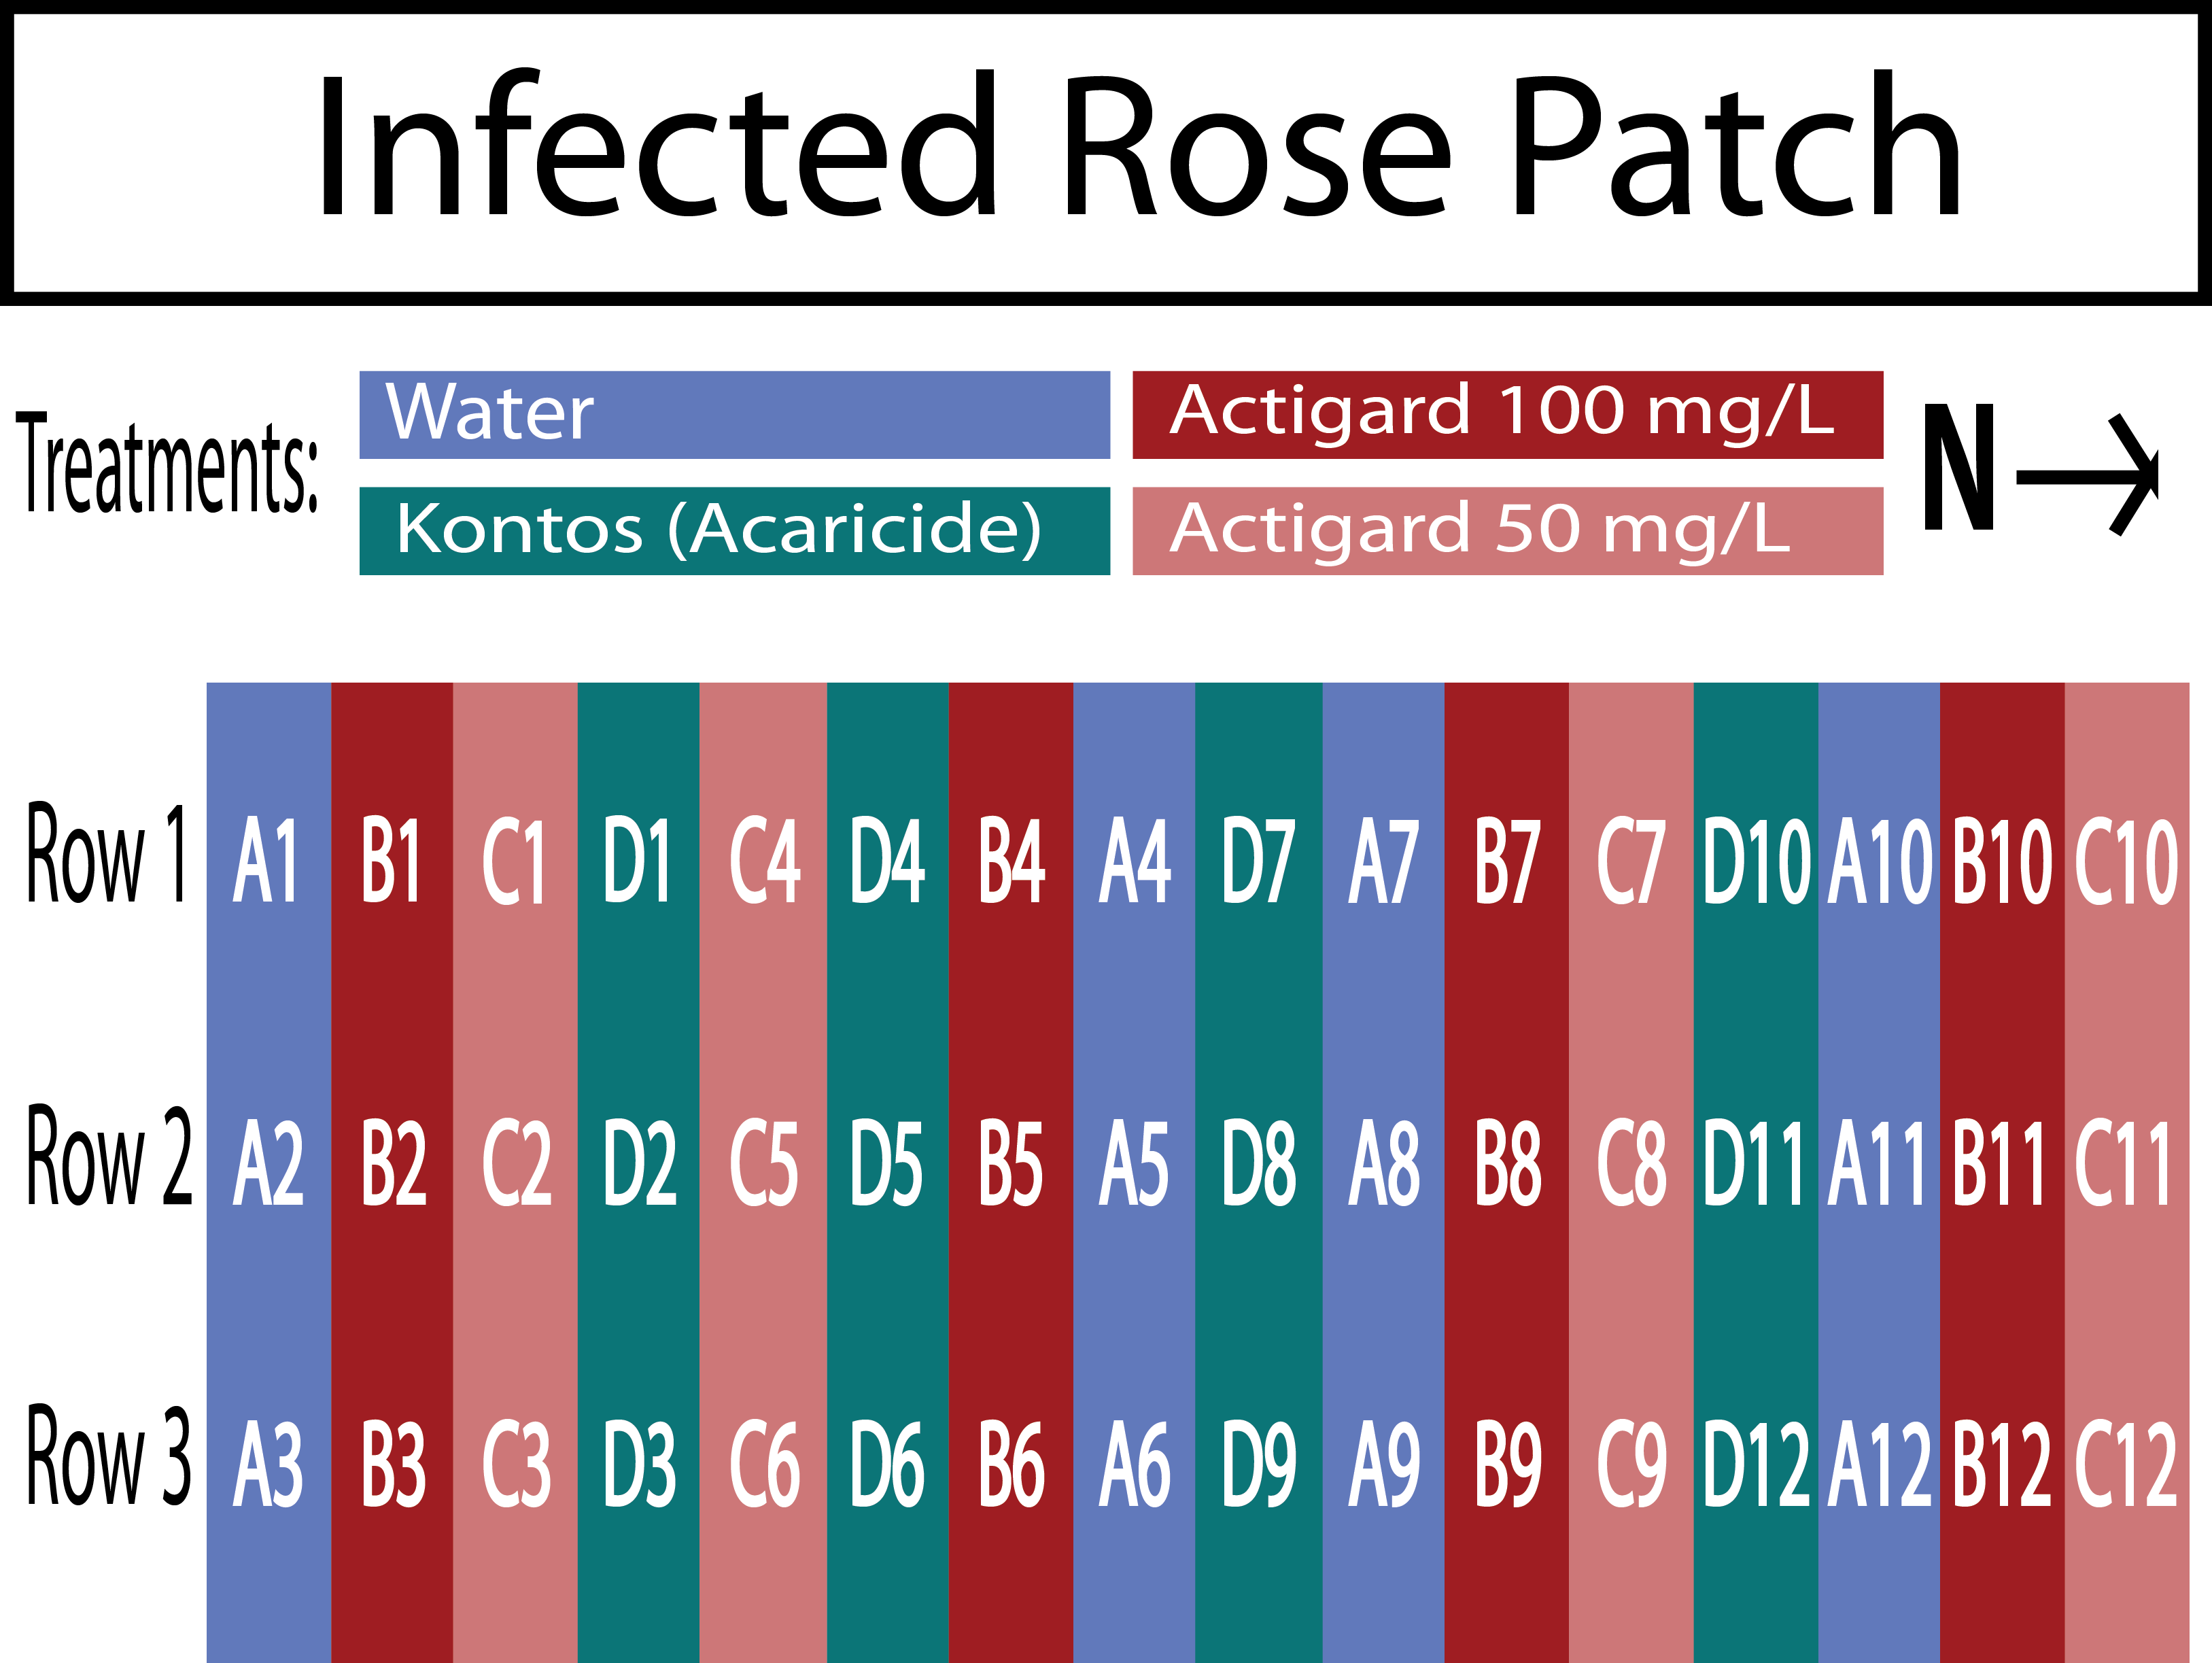
\includegraphics[width=1\linewidth]{figure/rrv_asm_plot_2018_griffin} 

}

\caption[Field design for testing the potential of acibenzolar-S-methyl (ASM) to reduce populations of \textit{P. fructiphilus}]{Field design for testing the potential of acibenzolar-S-methyl (ASM) to reduce populations of \textit{P. fructiphilus} by inducing Systemic Acquired Resistance (SAR) in Pink Double Knock Out® roses. Trials were conducted for three months from September to December 2019 in Griffin, GA. Four treatments were applied weekly fo 12 weeks: Blue = Water Red = Actigard50WG® 100 \si{\milli\gram}/L (High rate),  Pink = Actigard50WG® \si{\milli\gram}/L (Half rate) Turquoise = Kontos® (Label rate). Flower cuttings were be taken weekly to record \textit{P. fructiphilus} numbers.}\label{fig:grif-asm-2018}
\end{figure}
\textbf{Plot Design ASM Trials, Griffin - 2019}
\begin{figure}

{\centering 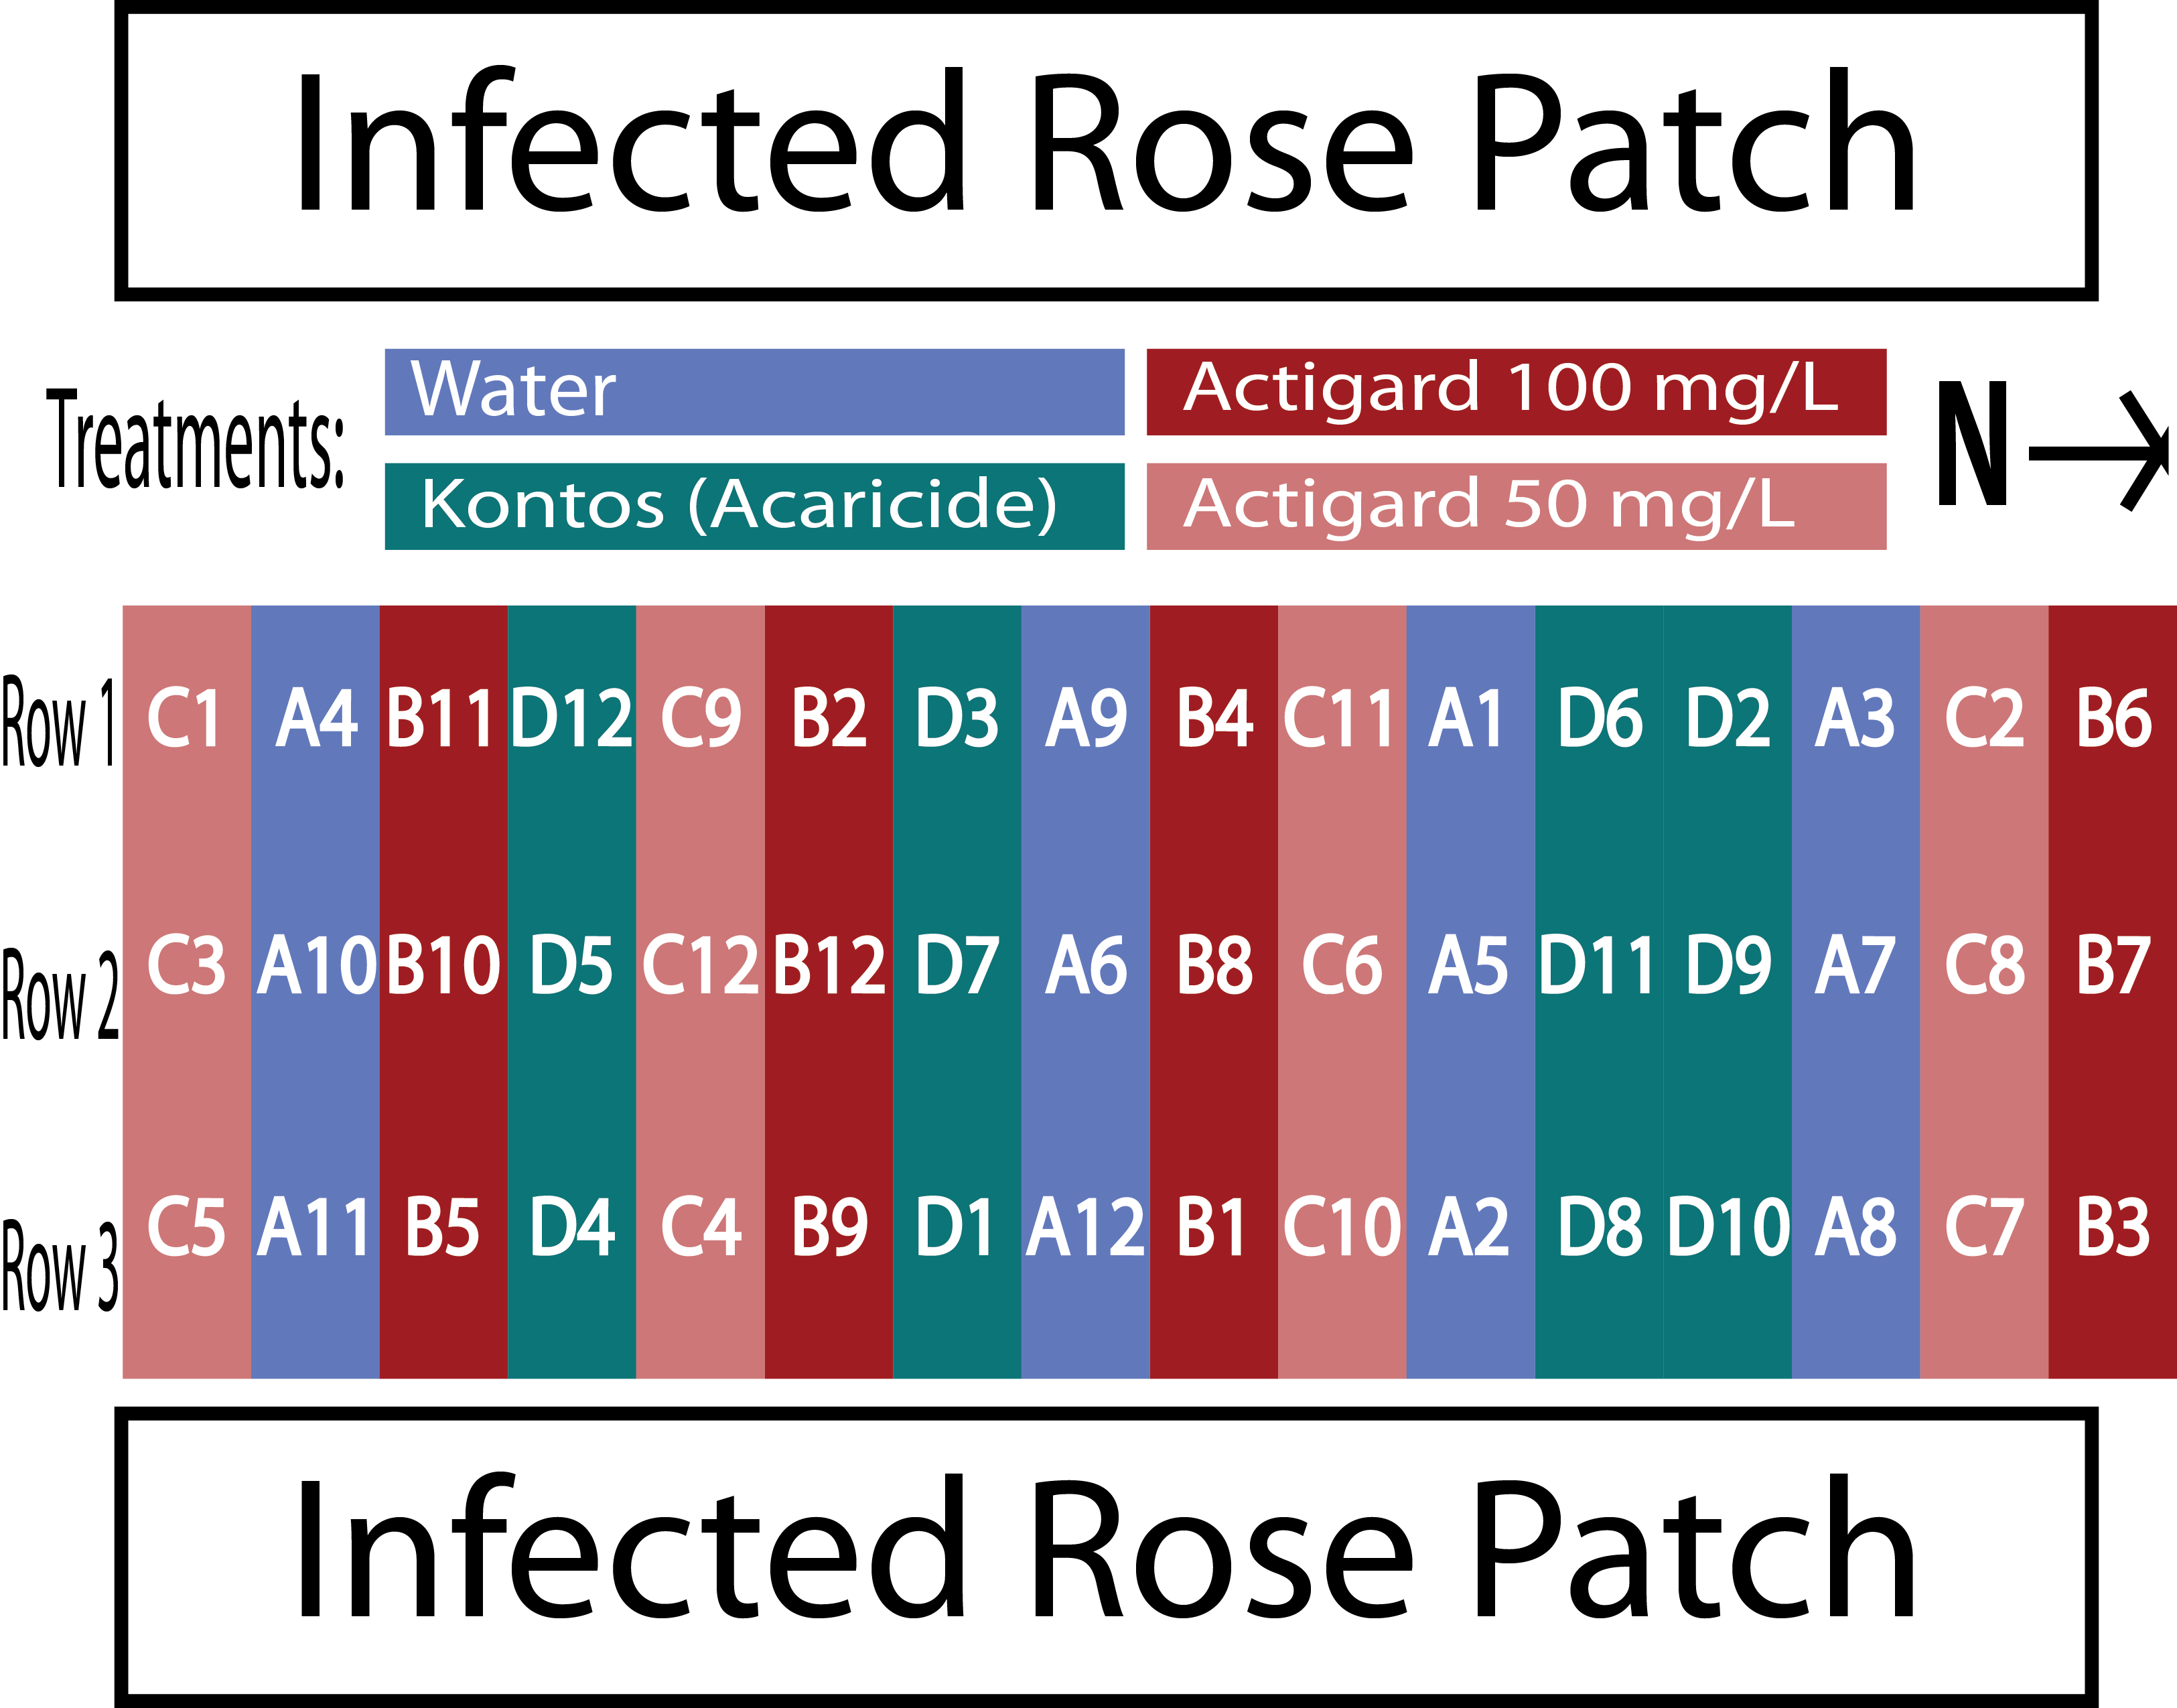
\includegraphics[width=1\linewidth]{figure/rrv_asm_plot_2019_griffin} 

}

\caption[Field design for testing the potential of ASM to reduce populations of \textit{P. fructiphilus}]{Field design for testing the potential of ASM to reduce populations of \textit{P. fructiphilus} by inducing SAR in Pink Double Knock Out® roses. Trials were conducted for three months from September to December 2019 in Griffin, GA. Four treatments were applied weekly fo 12 weeks: Blue = Water Red = Actigard50WG® 100 \si{\milli\gram}/L (High rate),  Pink = Actigard50WG® 100 \si{\milli\gram}/L (Half rate) Turquoise = Kontos® (Label rate). Flower cuttings were be taken weekly to record \textit{P. fructiphilus} numbers.}\label{fig:grif-asm-2019}
\end{figure}
\textbf{Data Collection for ASM Trials}
Rose/rosebud cuttings of about \textasciitilde10 cm of cane were taken from each rose before the first treatments to determine the initial populations of \emph{P. fructiphilus} on the roses. A stratified subset (one row across all blocks) of samples was taken from each rose treatment weekly, rotating samples until each rose plant has been sampled three times. Samples were collected from all roses at the end of the trial. The field trial was repeated for two seasons during the growing seasons of 2018 and 2019. Rose samples were placed in 50 mL centrifuge tubes and refrigerated or frozen until floral samples could be processed with 90\% ethanol according to the methods of Monfreda et al. (\protect\hyperlink{ref-Monfreda2007}{2007}). Eriophyoid mites and other mites collected were counted. Eriophyoid mites were identified after clearing and mounting in Hoyer's iodine-modified medium as described by Faraji and Bakker (\protect\hyperlink{ref-Faraji2008}{2008}).

\hypertarget{integrating-management-options-to-control-phyllocoptes-fructiphilus}{%
\subsection{\texorpdfstring{Integrating management options to control \emph{Phyllocoptes fructiphilus}}{Integrating management options to control Phyllocoptes fructiphilus}}\label{integrating-management-options-to-control-phyllocoptes-fructiphilus}}

During 2019 we conducted a second set of field trials in Griffin and Athens in addition to the ASM trials. We tested ASM alongside a different a SAR-inducer (SP2700, Trade name `Ninja', SePro) and combined this SAR-inducer with predatory mites releases to observe if these two treatments would have greater reductions of \emph{T. urticae} than either treatment on its own. We again tested a spirotetramat-based miticide and used water as a positive control (see \emph{\ref{fig:athens-ipm-2019}} and \emph{\ref{fig:griff-ipm-2019}}).

\textbf{Mite Infestation}
\emph{P. fructiphilus} are present in the landscape of Georgia. Cuttings of \textasciitilde10 cm or rose cane were taken from roses showing symptoms of RRD in the landscape and placed in each rose pot on the 1st, 5th and 9th weeks of the experiment.

\textbf{Predatory mites}
\emph{Amblyseius swirskii} predatory mites were applied/released on the 1st, 5th and 9th week of the experiments. Mites were deployed from polyethylene fiber sachets (Ambly-S, Arbico Organics, Oro Valley, AZ, USA), containing live colonies of \emph{A. swirskii} and a mite which they consume for food (\protect\hyperlink{ref-Midthassel2014}{Midthassel et al. 2014}). There is a small hole at the bottom of these sachets which allowed the mites to be slowly released into the environment. The sachets were hung from rose canes in the center of each rose canopy to encourage successful mite release (\protect\hyperlink{ref-Buitenhuis2014}{Buitenhuis et al. 2014}, \protect\hyperlink{ref-Addesso2018}{Addesso et al. 2018}).

\textbf{Roses}
The experiments were run for 12 weeks from August to October simultaneously in Griffin, GA and Athens, GA. Bare root roses were planted 2 months before the trials began to allow new flush to form. Rose planting media and environmental conditions were the same as previously described. The Athens site received and planted 96 Pink Double Knock Out® Roses (Star Roses and Plants, West Grove, PA, USA), while the Griffin site received 54 roses due to the smaller plot area available. The site at Athens had space for five blocks, while the site at Griffin, GA had space for three blocks. Each block was a 3 \(\times\) 6 plot with 18 plants, with three roses for each treatment. Flower cuttings were sampled from two rows each week, starting with the top rows of each block and rotating to the next row each week, continuing until all rows were sampled three times.

\textbf{Treatments}
Actigard50WG® (Syngenta, Greensboro, NC, USA), (acibenzolar-S-methyl, ASM) was applied at 100 \si{\milli\gram}/\si{\liter}, SP2700 (Trade name: Ninja\texttrademark, SePro, Carmel, IN, USA) was applied at its labeled rate, A spirotetramat based miticide was applied at the label rate (Kontos® Miticide Insecticide, Bayer Corporation, Whippany, New Jersey, USA), and tap water was used as a control. \emph{A. swirskii} mites were deployed with one sachet per rose treated, and \emph{A. swirskii} + Ninja treatments were applied with one sachet per rose treated, and SP2700 applied at its labelled rate. Treatments were done on the same day each week, weather permitting. Trials in Athens had the same treatments.

\textbf{Plot Design - Athens IPM 2019}
\begin{figure}

{\centering 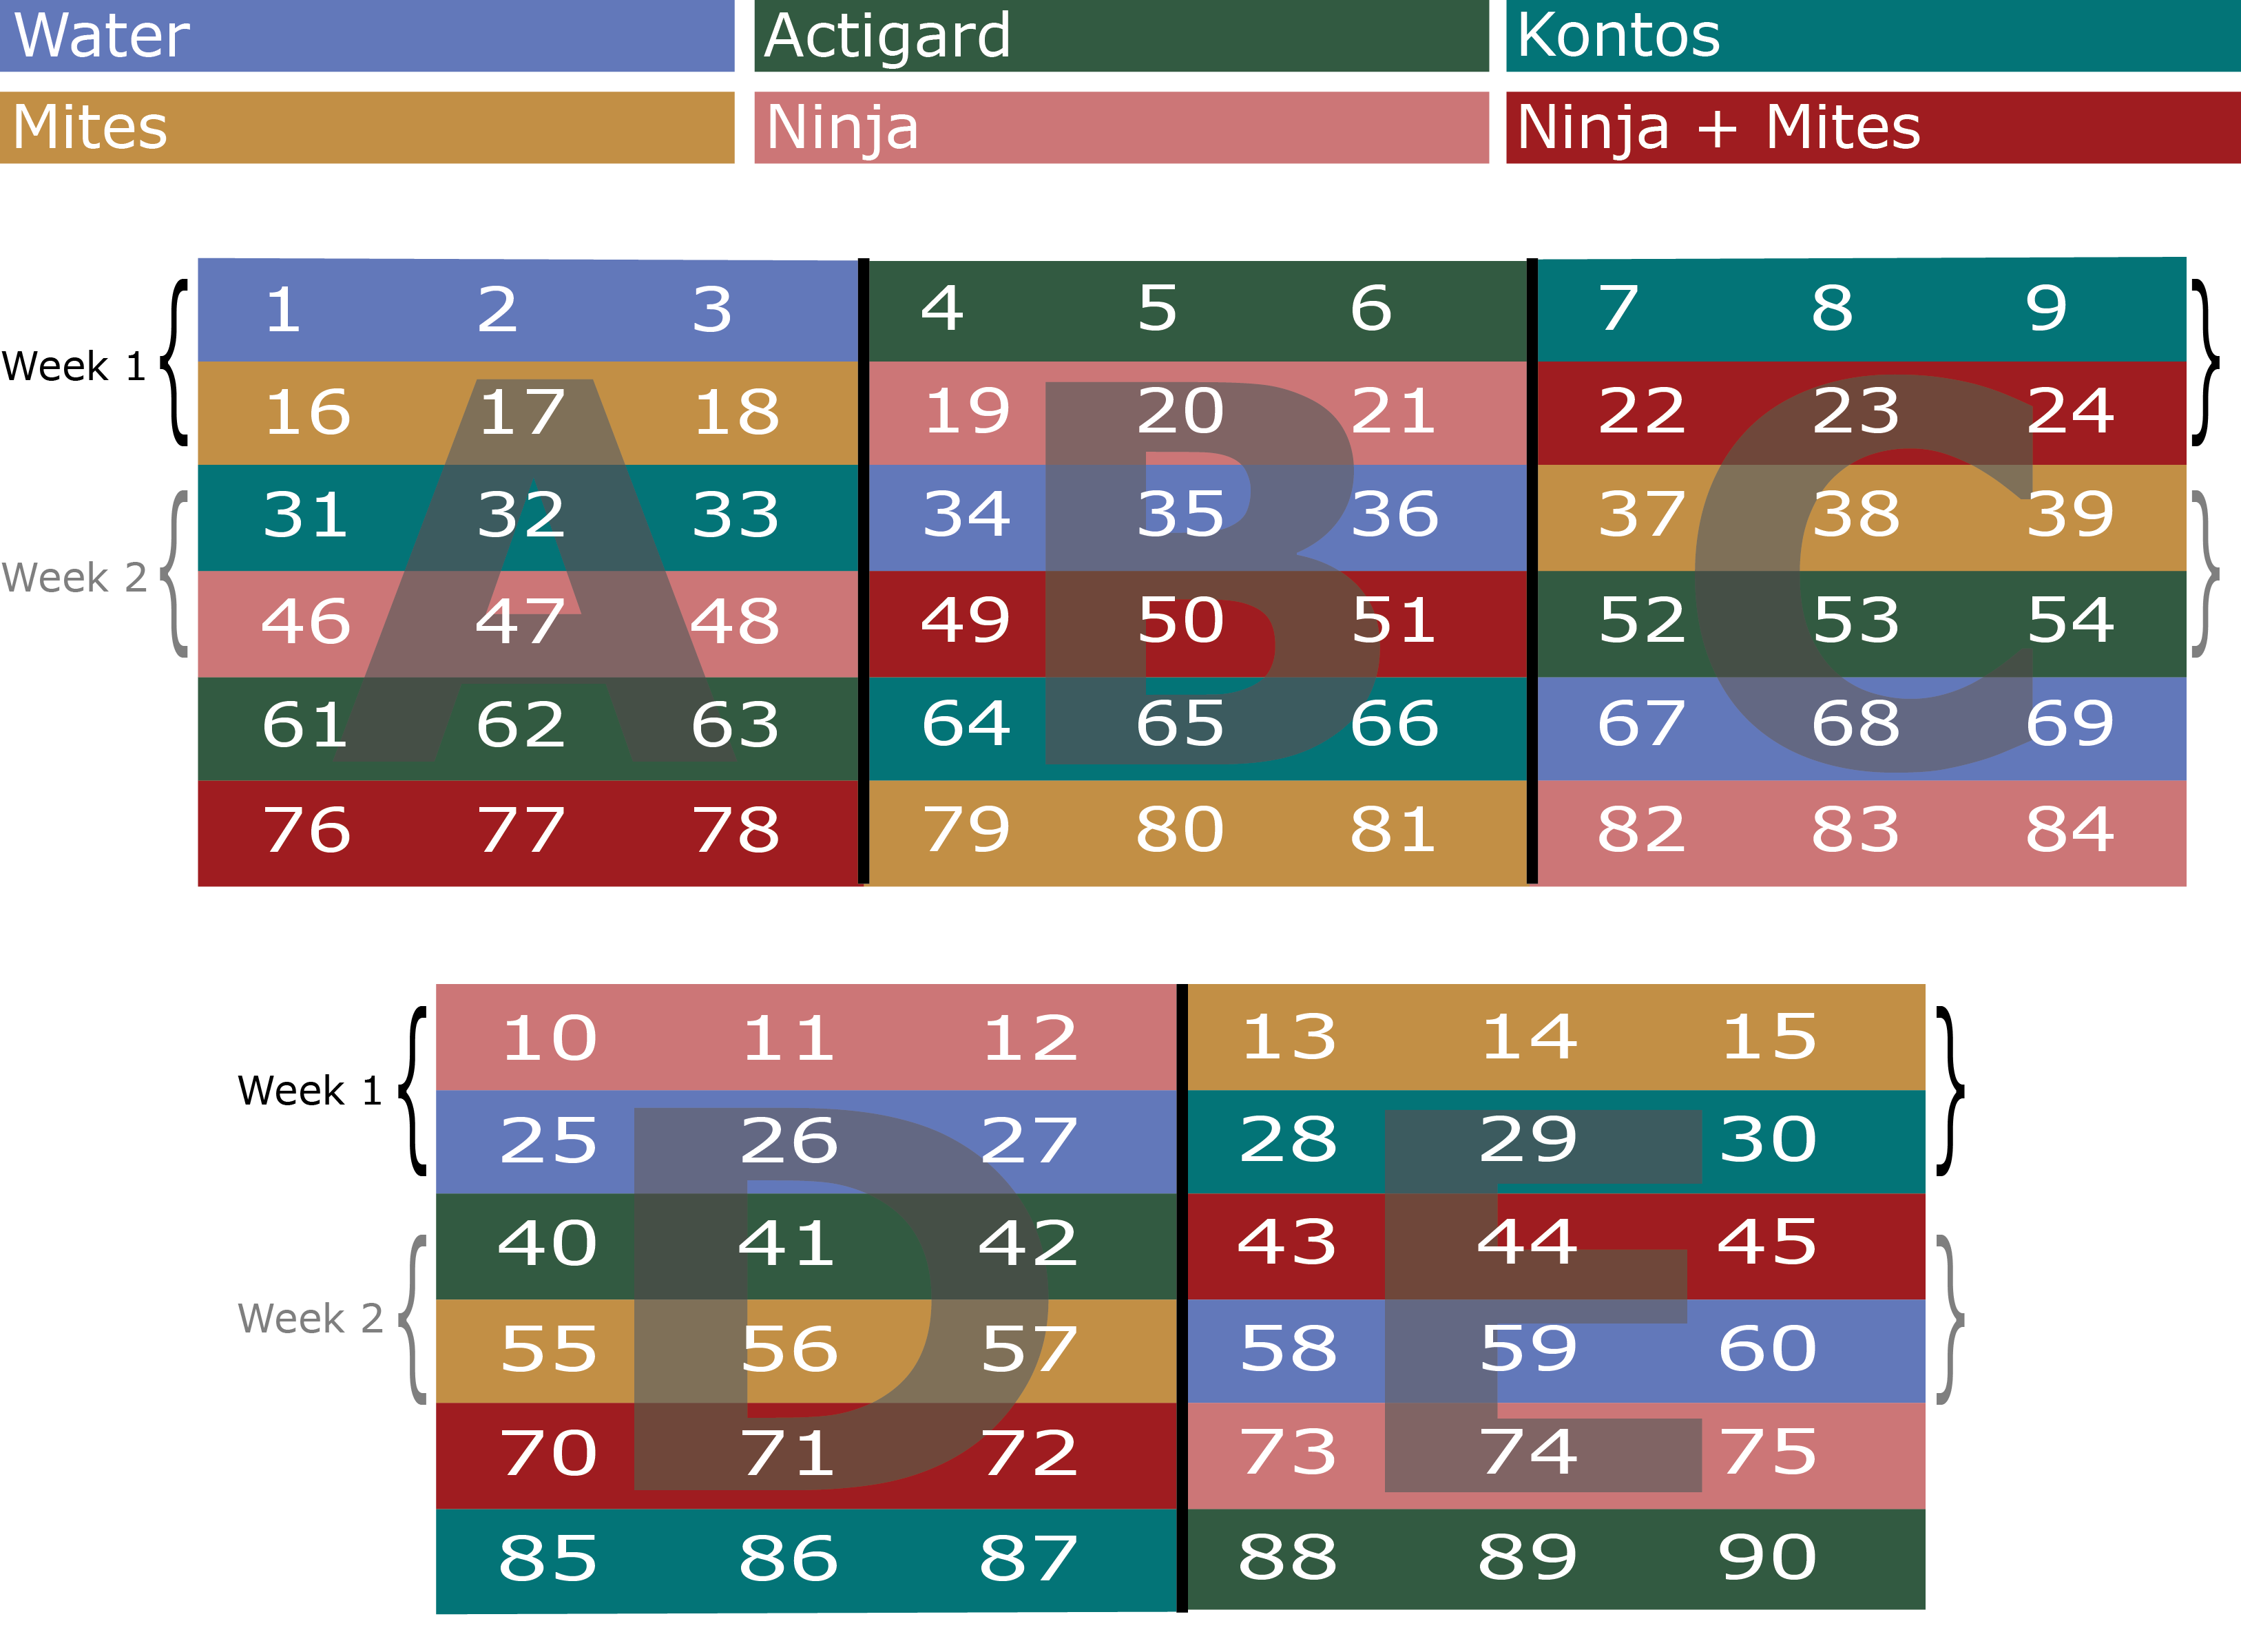
\includegraphics[width=1\linewidth]{figure/rrv_ipm_plot_map_2019_athens} 

}

\caption[Field design for Integrated Pest Management (IPM) trials on Pink Double Knock Out® roses to control \textit{P. fructiphilus} in Athens, GA with five treatments]{Field design for Integrated Pest Management (IPM) trials on Pink Double Knock Out® roses to control \textit{P. fructiphilus} in Athens, GA with five treatments. W = Water A = Actigard50WG, K = Kontos®, M = \textit{A. swirkii} predatory mite sachets, N = SP2700 (Trade name: Ninja, SePro), + = \textit{A. swirskii} + Ninja combined treatments. All products were applied at their label rates for 12 weeks. Flower cuttings were taken weekly to record \textit{P. fructiphilus} numbers.}\label{fig:athens-ipm-2019}
\end{figure}
\textbf{Plot Design - Griffin IPM 2019}
\begin{figure}

{\centering 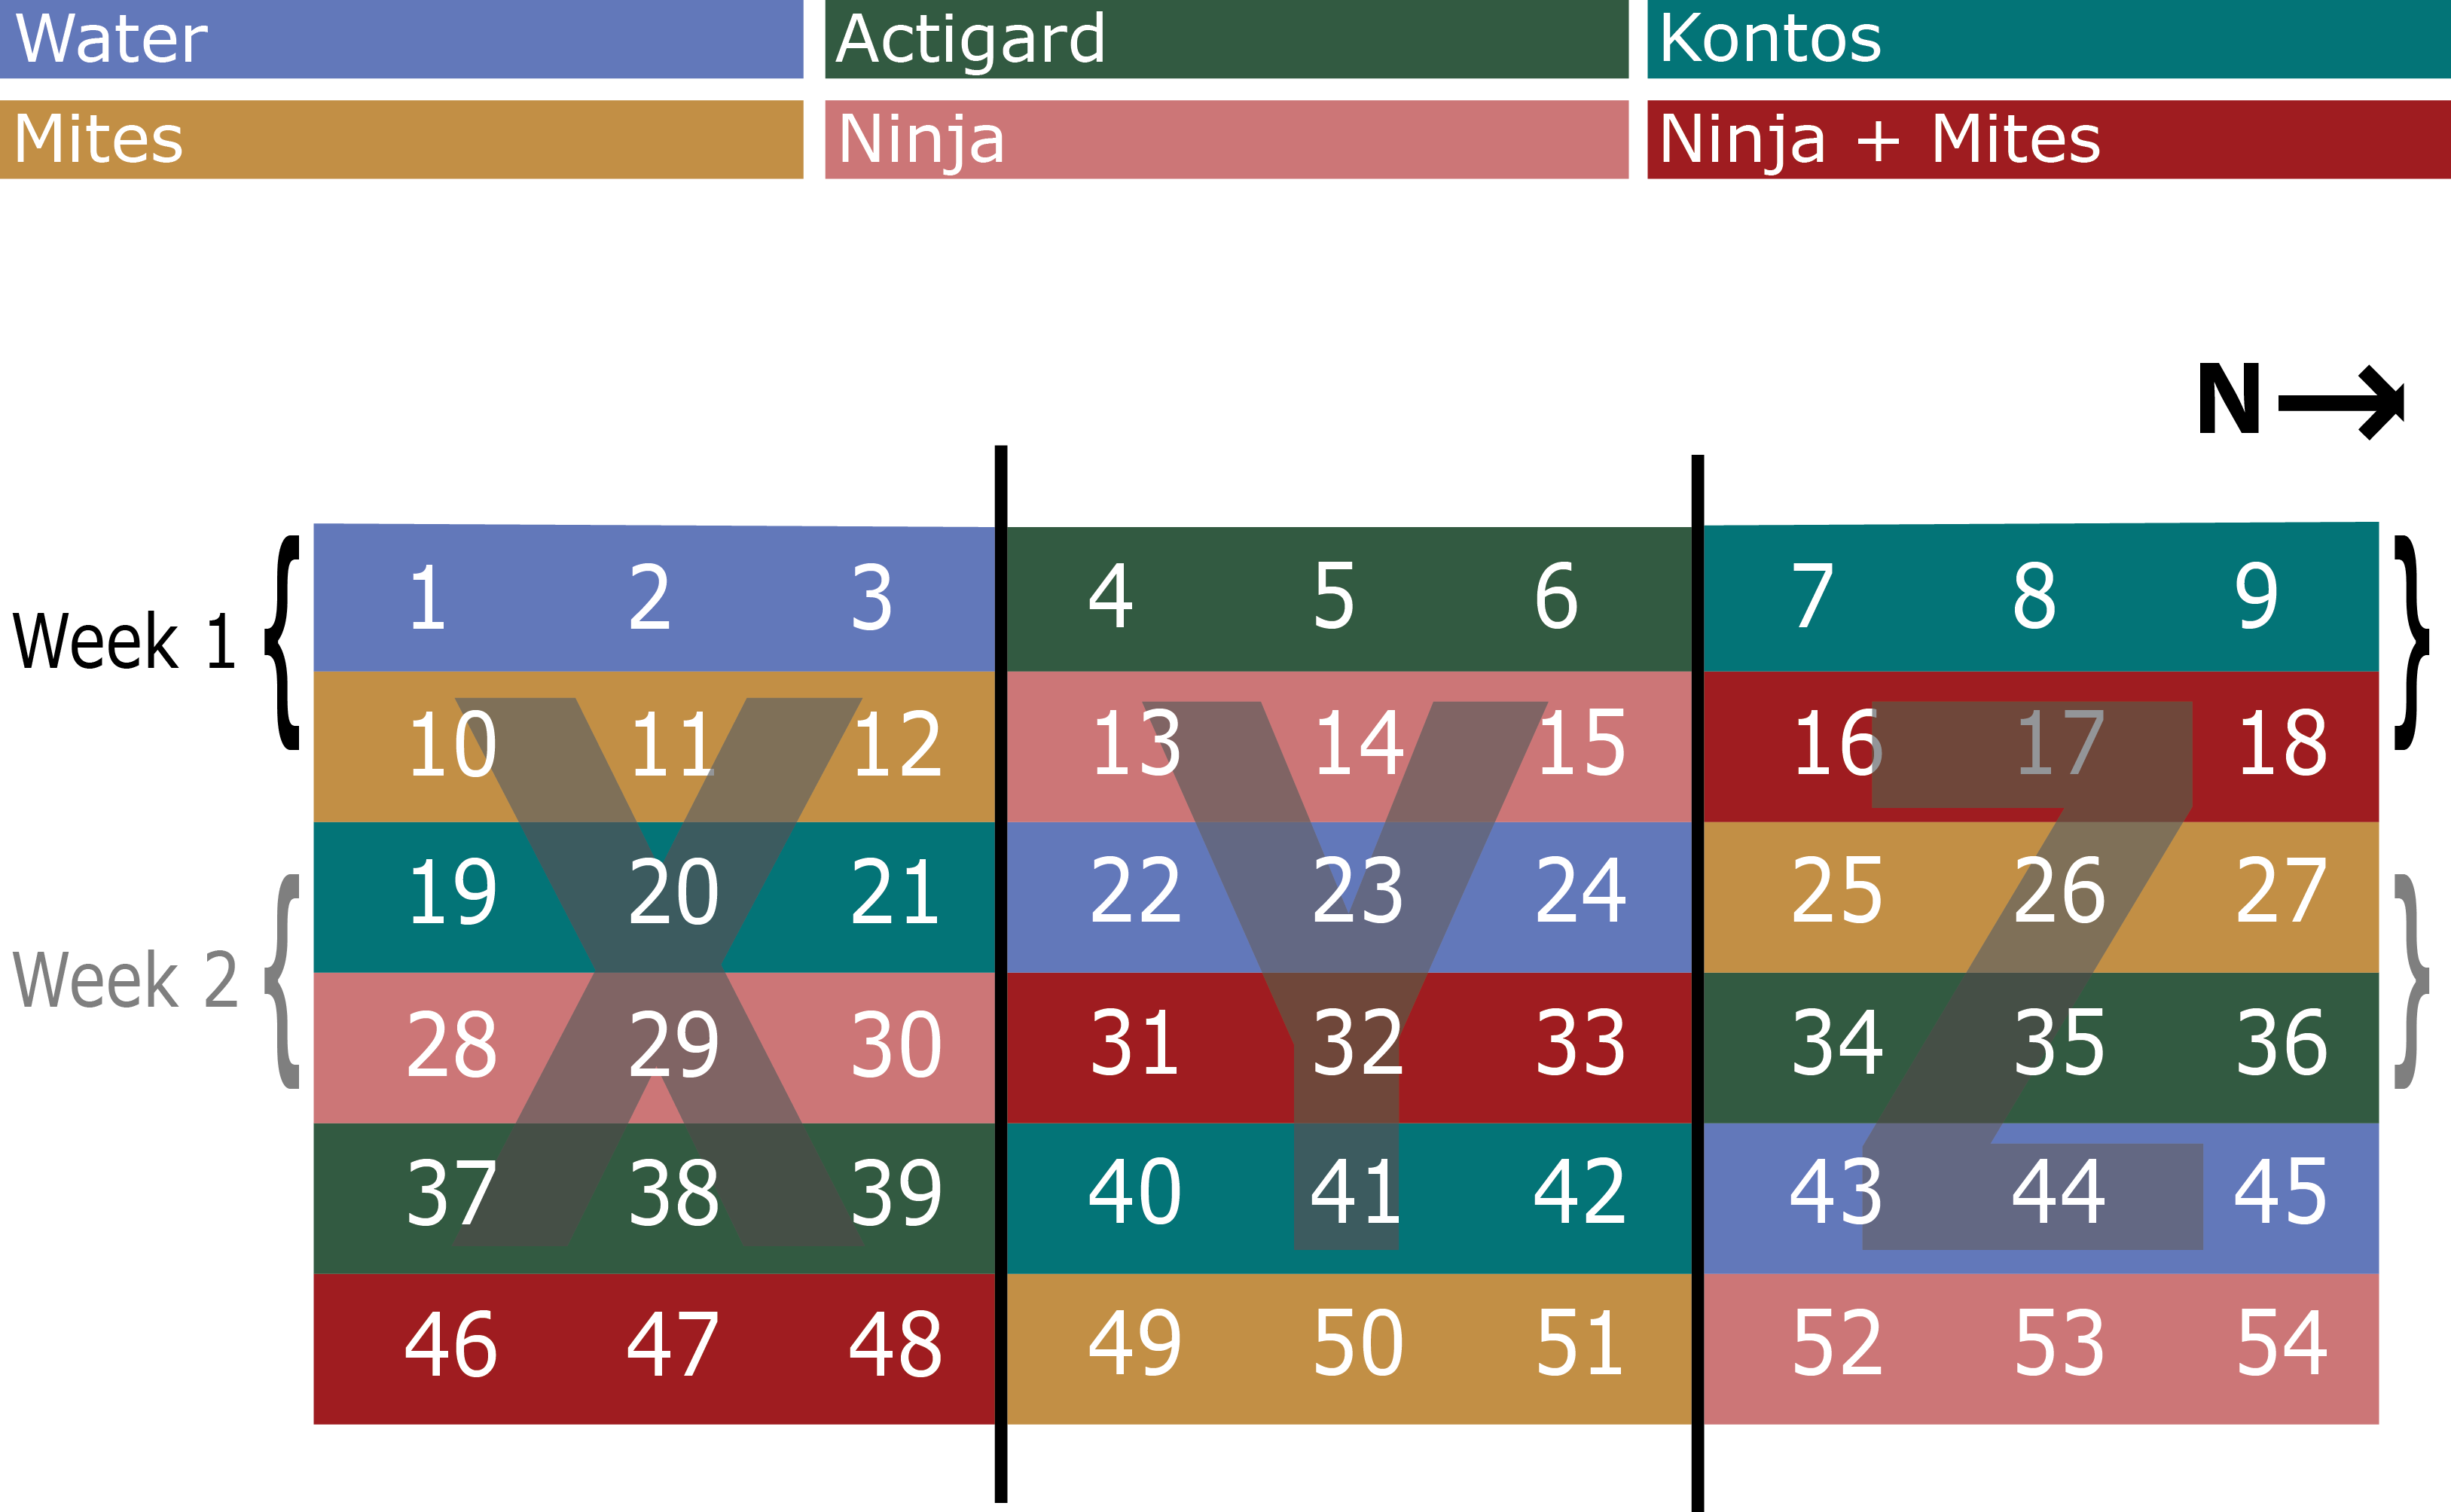
\includegraphics[width=1\linewidth]{figure/rrv_ipm_plot_map_2019_griffin} 

}

\caption[Field design for IPM trials on Pink Double Knock Out® roses to control \textit{P. fructiphilus} in Griffin, GA with five treatments]{Field design for IPM trials on Pink Double Knock Out® roses to control \textit{P. fructiphilus} in Griffin, GA with five treatments. W = Water A = Actigard50WG, K = Kontos®, M = \textit{A. swirkii} predatory mite sachets, N = SP2700 (Trade name: Ninja, SePro), + = \textit{A. swirskii} + Ninja combined treatments. All products were applied at their label rates for 12 weeks. Flower cuttings were taken weekly to record \textit{P. fructiphilus} numbers.}\label{fig:griff-ipm-2019}
\end{figure}
\textbf{Data Collection for Georgia IPM Trials}
Flower samples were collected from all roses once before beginning the treatments on week 1 and once at the end of the experiment on week 12. For weeks 2 through 11, flower samples were collected weekly. starting from the top rows of each block, until each row was sampled three times (see \emph{\ref{fig:athens-ipm-2019}} and \emph{\ref{fig:griff-ipm-2019}}). Disease severity was recorded weekly according to the Horsfall-Barratt Scale (\protect\hyperlink{ref-Horsfall1945}{Horsfall 1945}). Roses displaying symptoms of RRD had tissues sent to the Plant Disease Diagnostic Clinic at the North Florida Reasearch and Extension Center(PDC) for virus confirmation. Flower cuttings of about \textasciitilde12 cm were taken and placed in 50 ml centrifuge tubes. Flowers were placed flower side down and submerged with 15 ml of 95\% ethanol. Once the lid was secured, the the tube was shaken vigorously for a few seconds to help dislodge any mites. Samples were processed using the washing methods of Monfreda et al. (\protect\hyperlink{ref-Monfreda2007}{2007}), eriophyoid mites were counted and identified as previously described.

\hypertarget{phenology-field-study}{%
\subsection{Phenology field study}\label{phenology-field-study}}

In order to be sure that a further series of IPM trials would be successful, we monitored a population of \emph{P. fructiphilus} in Tallahassee which had mites but no RRD. Rose cuttings were collected periodically from four plots in the landscape of a church in Leon County, FL from 2020-2021: The site had two plantings of 2-3 years old Double Pink Knockout roses, with open sun exposure, \textasciitilde0.3 \si{\metre} spacing, and natural watering. Blocks were divided into 24 plots of \textasciitilde3 \si{\metre}\(^2\), with approximately 12 roses per plot. Samples were processed as previously described in \ref{materials-methods}. After washing, plant tissues were placed into in paper bags and put into a drying oven for \textasciitilde48 hrs at 50 °C, after which dry weight was recorded. Mites were counted and recorded to track changes in the mite populations. Roses were pruned once on the beginning of July 2020 by a professional landscaping crew.

\hypertarget{ipm-field-trials-tallahassee-2021}{%
\subsection{IPM field trials, Tallahassee 2021}\label{ipm-field-trials-tallahassee-2021}}

A second trial of IPM was conducted in Tallahassee, FL. This site did not have RRD present, but had verified populations of \emph{P. fructiphilus} present in the landscape (see APPENDIX). Spray applications were done weekly for 12 weeks from May to August 2021. Treatments were made on the same day each week, weather permitting.

\textbf{Roses}
The site was divided into two blocks, with ten plots of roses in each block. Each plot was 3 \si{m}\(^2\) with approximately 12 roses, the six roses at the center of the plot were treated, while the adjacent roses on either side was left as a buffer between plots to avoid treatment drift.

\textbf{Treatments}
Five treatments were applied: tap water as a control, Actigard50WG® (acibenzolar-S-methyl, Syngenta, Greensboro, NC, USA) - 100 \si{\milli\gram}/\si{\liter}, \emph{Amblyseius swirskii} mini sachets with hooks (Ambly-S, Arbico Organics, Oro Valley, AZ, USA) - two sachets per rose in treated plots, and a combined treatment of Actigard50WG® - 100 \si{\milli\gram}/\si{\liter} + \emph{A. swirskii} - two sachets per rose in treated plots, and a spirotetramat miticide (Kontos® Miticide Insecticide, Bayer Corporation, Whippany, New Jersey, USA), (see \emph{@(talla-ipm-2021)}).

\textbf{Mite Infestation}
\emph{P. fructiphilus} are present in the landscape of Tallahassee. Populations were present on the roses, as verified by the phenology experiments.

\textbf{Predatory mites}
The two sachets of \emph{A. swirskii} mites were applied to each of the six treated roses on the 1st, 5th and 9th week of the experiment, following the application instructions from the supplying company (Ambly-S, Arbico Organics, Oro Valley, AZ, USA). The sachets were hung from rose canes in the center of each rose. The \emph{A. swirskii} plots were also treated with water weekly when the other plots were sprayed in order to keep conditions similar to other treatments.

\textbf{Data Collection for Tallahassee IPM Trials}
Samples were collected and processed using similar methods as previously described in \ref{materials-methods}: Flower cuttings were taken weekly from from each of the six roses in the center of each plot. Three flowers (or buds if no flowers were present) were taken from each of the six central roses in each plot, for a total of 18 flowers/buds per bottle for each sampling bottle.The flowers/buds were placed into the ethanol-filled bottles and shaken vigorously for a few seconds to coat the rose tissue with ethanol and help dislodge any mites. Plant samples were processed according to the methods described in Monfreda et al. (\protect\hyperlink{ref-Monfreda2007}{2007}). Plant tissues were retained after mites were washed off, and dried in kraft paper bags and put into the oven until dry (\textasciitilde48 hrs at 50 °C), after which the dry weight of the rose tissues was recorded.
\begin{figure}

{\centering \includegraphics[width=1\linewidth]{thesis_files/figure-latex/talla-ipm-2021-1} 

}

\caption[Field design for IPM trials on Pink Double Knock Out® roses to control \textit{P. fructiphilus} in Tallahassee, FL with five treatments]{Field design for IPM trials on Pink Double Knock Out® roses to control \textit{P. fructiphilus} in Tallahassee, FL with five treatments: Water, Actigard50WG®, Kontos®, \textit{Amblyseius swirkii} predatory mite sachets, and \textit{A. swirskii} + Actigard combined treatments. All products were applied at their label rates for 12 weeks. Flower cuttings were taken weekly to record \textit{P. fructiphilus} numbers.}\label{fig:talla-ipm-2021}
\end{figure}
\hypertarget{analysis-of-field-trial-data}{%
\subsection{Analysis of field trial data}\label{analysis-of-field-trial-data}}

All data from all trials was processed and analyzed using R version 4.1.1 (\protect\hyperlink{ref-RCT2021}{R Core Team 2021}). The data were all count data, so a Zero-Inflated Poisson Model (\protect\hyperlink{ref-Zeileis2008}{Zeileis et al. 2008}) was required for the ASM data (\protect\hyperlink{ref-Hothorn2008}{Hothorn et al. 2008}), while Generalized Linear Mixed Models (\protect\hyperlink{ref-Bates2015}{Bates et al. 2015}) were used for all of the IPM and phenology trials. Estimated marginal means (least squares means) (\protect\hyperlink{ref-Lenth2021}{Lenth 2021}) and Tukey Contrasts Multiple Comparisons of Means were used to determine significant effects. In addition, about \textasciitilde5\% of early samples collected from the Tallahassee field trials were missing dry weights. Missing weight data was estimated and imputted using Multivariate Imputation by Chained Equations via the mice package (\protect\hyperlink{ref-vanBuuren2011}{Buuren and Groothuis-Oudshoorn 2011}).

\hypertarget{results-2}{%
\section{Results}\label{results-2}}

\hypertarget{asm-trials}{%
\subsection{ASM trials}\label{asm-trials}}
\begin{figure}

{\centering 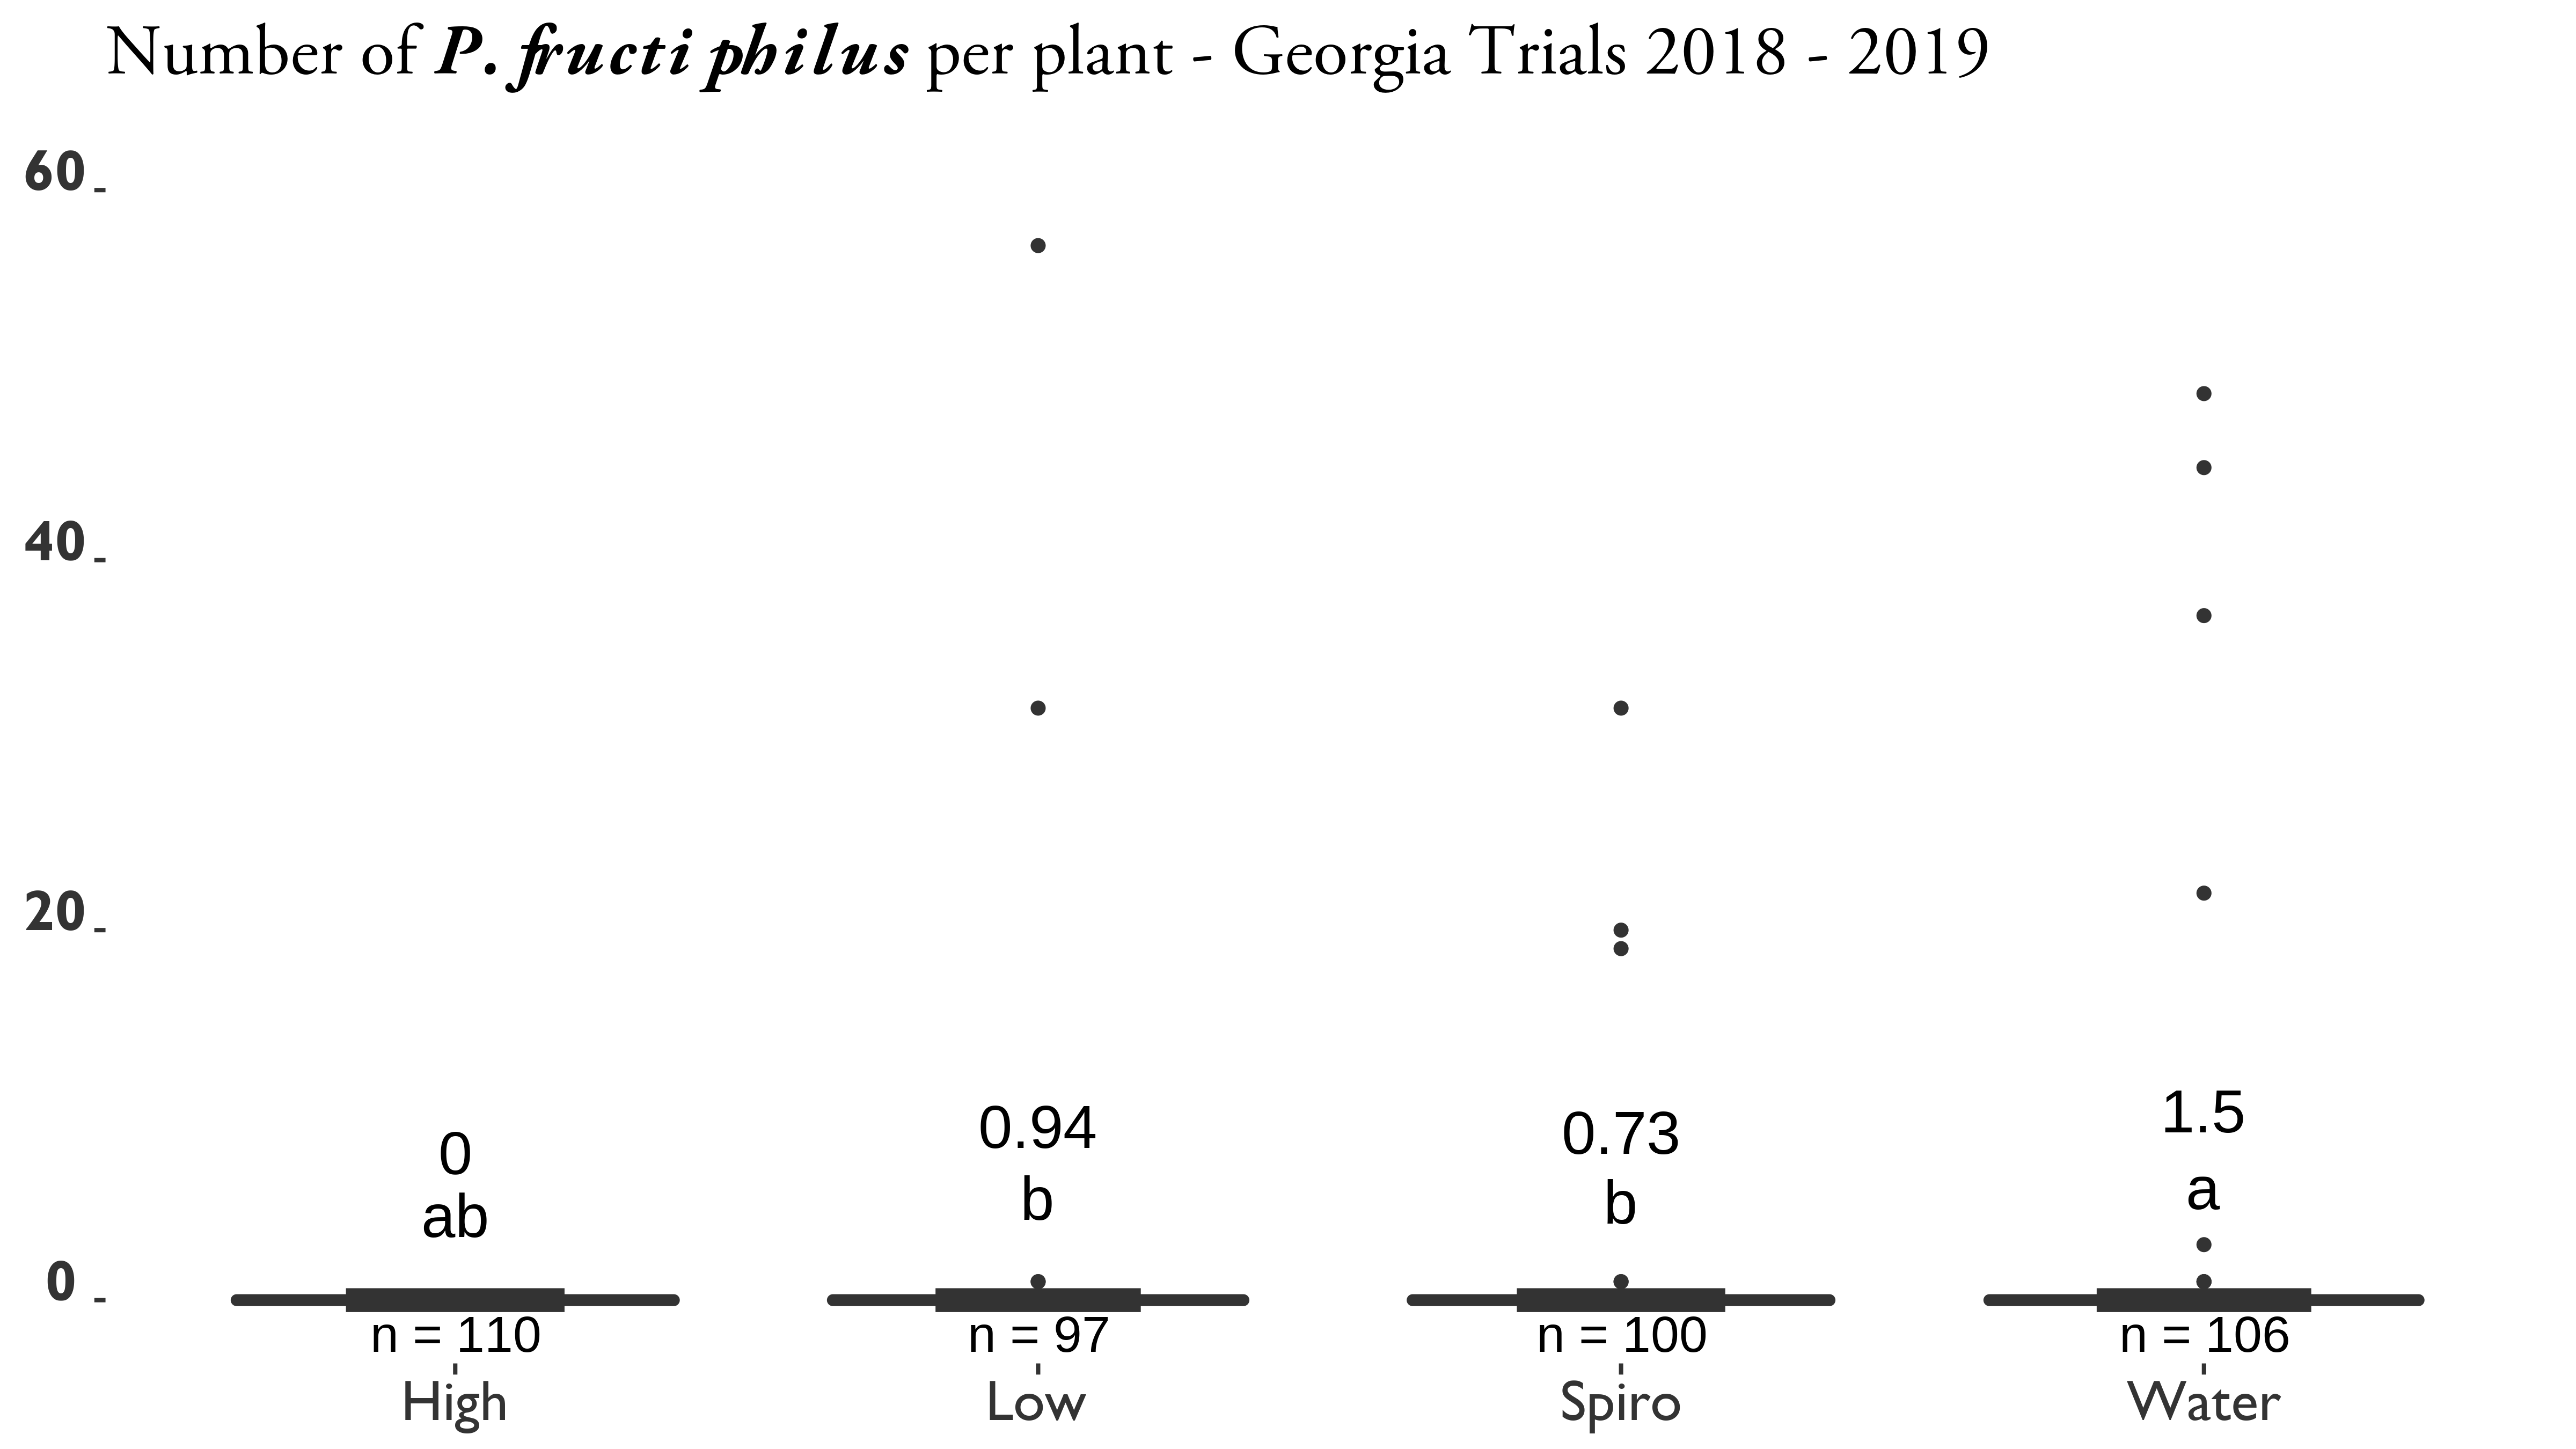
\includegraphics[width=1\linewidth]{figure/rrv_actigard_graph} 

}

\caption[SAR-induction trials on Pink Double Knock Out® roses to control \textit{Phyllocoptes fructiphilus} in Athens and Griffin, GA]{SAR-induction trials on Pink Double Knock Out® roses to control \textit{Phyllocoptes fructiphilus} in Athens and Griffin, GA. Statistical significance was determined using Tukey contrasts for multiple Comparisons of means. Groups which share letters are not statistically different from one another. $\alpha = 0.05$. water = Water Control, High = 100 \si{\milli\gram}/\si{\liter} Actigard50WG® (Syngenta, Greensboro, NC, USA) acibenzolar-S-methyl (ASM), low = 50 \si{\milli\gram}/\si{\liter} Actigard50WG® (Syngenta, Greensboro, NC, USA) acibenzolar-S-methyl (ASM), Spiro = Kontos® Miticide Insecticide - Spirotetramat (Bayer Corporation, Whippany, New Jersey, USA), All products were applied for 12 weeks. Flower cuttings were taken weekly to record the numbers of herbivorous mites.}\label{fig:asm-graph}
\end{figure}
\begin{landscape}\begin{table}

\caption{\label{tab:asm-athns-2018-table}Progression of RRD on SAR-induced Pink Double Knock Out® roses in Athens, GA 2018.}
\centering
\resizebox{\linewidth}{!}{
\begin{tabular}[t]{lrrrrrrrrrrrrrrrllrrl}
\toprule
Treatment & Block & 2018-08-31 & 2018-09-07 & 2018-09-14 & 2018-09-21 & 2018-09-28 & 2018-10-05 & 2018-10-12 & 2018-10-19 & 2018-10-26 & 2018-11-02 & 2018-12-19 & AUDPC & Final disease severity (\%) & Sample \# & Plant & RRD & P.fructiphilus & Other Mites & Field\\
\midrule
\cellcolor{gray!6}{Water} & \cellcolor{gray!6}{1} & \cellcolor{gray!6}{0} & \cellcolor{gray!6}{0} & \cellcolor{gray!6}{0} & \cellcolor{gray!6}{0.0} & \cellcolor{gray!6}{0.0} & \cellcolor{gray!6}{0.0} & \cellcolor{gray!6}{1.5} & \cellcolor{gray!6}{1.5} & \cellcolor{gray!6}{4.5} & \cellcolor{gray!6}{1.5} & \cellcolor{gray!6}{17.5} & \cellcolor{gray!6}{124.25} & \cellcolor{gray!6}{17.5} & \cellcolor{gray!6}{1} & \cellcolor{gray!6}{W1} & \cellcolor{gray!6}{S} & \cellcolor{gray!6}{2} & \cellcolor{gray!6}{0} & \cellcolor{gray!6}{Athens}\\
Water & 2 & 0 & 0 & 0 & 0.0 & 0.0 & 0.0 & 0.0 & 1.5 & 4.5 & 1.5 & 0.0 & 52.50 & 0.0 & 2 & W2 & A? & 0 & 0 & Athens\\
\cellcolor{gray!6}{Water} & \cellcolor{gray!6}{3} & \cellcolor{gray!6}{0} & \cellcolor{gray!6}{0} & \cellcolor{gray!6}{0} & \cellcolor{gray!6}{0.0} & \cellcolor{gray!6}{0.0} & \cellcolor{gray!6}{0.0} & \cellcolor{gray!6}{0.0} & \cellcolor{gray!6}{1.5} & \cellcolor{gray!6}{4.5} & \cellcolor{gray!6}{1.5} & \cellcolor{gray!6}{1.5} & \cellcolor{gray!6}{57.75} & \cellcolor{gray!6}{1.5} & \cellcolor{gray!6}{3} & \cellcolor{gray!6}{W3} & \cellcolor{gray!6}{A} & \cellcolor{gray!6}{0} & \cellcolor{gray!6}{0} & \cellcolor{gray!6}{Athens}\\
Water & 4 & 0 & 0 & 0 & 0.0 & 0.0 & 0.0 & 1.5 & 1.5 & 0.0 & 1.5 & 0.0 & 31.50 & 0.0 & 4 & W4 & A & 0 & 0 & Athens\\
\cellcolor{gray!6}{Water} & \cellcolor{gray!6}{5} & \cellcolor{gray!6}{0} & \cellcolor{gray!6}{0} & \cellcolor{gray!6}{0} & \cellcolor{gray!6}{0.0} & \cellcolor{gray!6}{0.0} & \cellcolor{gray!6}{0.0} & \cellcolor{gray!6}{1.5} & \cellcolor{gray!6}{1.5} & \cellcolor{gray!6}{0.0} & \cellcolor{gray!6}{0.0} & \cellcolor{gray!6}{9.0} & \cellcolor{gray!6}{52.50} & \cellcolor{gray!6}{9.0} & \cellcolor{gray!6}{5} & \cellcolor{gray!6}{W5} & \cellcolor{gray!6}{S} & \cellcolor{gray!6}{0} & \cellcolor{gray!6}{0} & \cellcolor{gray!6}{Athens}\\
\addlinespace
Water & 6 & 0 & 0 & 0 & 0.0 & 0.0 & 0.0 & 1.5 & 1.5 & 1.5 & 1.5 & 9.0 & 73.50 & 9.0 & 6 & W6 & S & 1 & 1 & Athens\\
\cellcolor{gray!6}{Water} & \cellcolor{gray!6}{7} & \cellcolor{gray!6}{0} & \cellcolor{gray!6}{0} & \cellcolor{gray!6}{0} & \cellcolor{gray!6}{0.0} & \cellcolor{gray!6}{0.0} & \cellcolor{gray!6}{0.0} & \cellcolor{gray!6}{0.0} & \cellcolor{gray!6}{0.0} & \cellcolor{gray!6}{1.5} & \cellcolor{gray!6}{1.5} & \cellcolor{gray!6}{1.5} & \cellcolor{gray!6}{26.25} & \cellcolor{gray!6}{1.5} & \cellcolor{gray!6}{7} & \cellcolor{gray!6}{W7} & \cellcolor{gray!6}{A} & \cellcolor{gray!6}{0} & \cellcolor{gray!6}{0} & \cellcolor{gray!6}{Athens}\\
Water & 8 & 0 & 0 & 0 & 0.0 & 0.0 & 0.0 & 0.0 & 0.0 & 1.5 & 1.5 & 4.5 & 36.75 & 4.5 & 8 & W8 & A? & 0 & 0 & Athens\\
\cellcolor{gray!6}{Water} & \cellcolor{gray!6}{9} & \cellcolor{gray!6}{0} & \cellcolor{gray!6}{0} & \cellcolor{gray!6}{0} & \cellcolor{gray!6}{0.0} & \cellcolor{gray!6}{0.0} & \cellcolor{gray!6}{0.0} & \cellcolor{gray!6}{1.5} & \cellcolor{gray!6}{1.5} & \cellcolor{gray!6}{1.5} & \cellcolor{gray!6}{1.5} & \cellcolor{gray!6}{0.0} & \cellcolor{gray!6}{42.00} & \cellcolor{gray!6}{0.0} & \cellcolor{gray!6}{9} & \cellcolor{gray!6}{W9} & \cellcolor{gray!6}{A} & \cellcolor{gray!6}{0} & \cellcolor{gray!6}{0} & \cellcolor{gray!6}{Athens}\\
Water & 10 & 0 & 0 & 0 & 0.0 & 0.0 & 0.0 & 0.0 & 1.5 & 1.5 & 1.5 & 0.0 & 31.50 & 0.0 & 10 & W10 & A? & 0 & 0 & Athens\\
\addlinespace
\cellcolor{gray!6}{Water} & \cellcolor{gray!6}{11} & \cellcolor{gray!6}{0} & \cellcolor{gray!6}{0} & \cellcolor{gray!6}{0} & \cellcolor{gray!6}{0.0} & \cellcolor{gray!6}{0.0} & \cellcolor{gray!6}{1.5} & \cellcolor{gray!6}{0.0} & \cellcolor{gray!6}{0.0} & \cellcolor{gray!6}{1.5} & \cellcolor{gray!6}{1.5} & \cellcolor{gray!6}{1.5} & \cellcolor{gray!6}{36.75} & \cellcolor{gray!6}{1.5} & \cellcolor{gray!6}{11} & \cellcolor{gray!6}{W11} & \cellcolor{gray!6}{A?} & \cellcolor{gray!6}{0} & \cellcolor{gray!6}{0} & \cellcolor{gray!6}{Athens}\\
Water & 12 & 0 & 0 & 0 & 0.0 & 0.0 & 0.0 & 1.5 & 1.5 & 1.5 & 1.5 & 17.5 & 103.25 & 17.5 & 12 & W12 & S & 0 & 1 & Athens\\
\cellcolor{gray!6}{Low} & \cellcolor{gray!6}{1} & \cellcolor{gray!6}{0} & \cellcolor{gray!6}{0} & \cellcolor{gray!6}{0} & \cellcolor{gray!6}{0.0} & \cellcolor{gray!6}{0.0} & \cellcolor{gray!6}{0.0} & \cellcolor{gray!6}{0.0} & \cellcolor{gray!6}{1.5} & \cellcolor{gray!6}{4.5} & \cellcolor{gray!6}{1.5} & \cellcolor{gray!6}{0.0} & \cellcolor{gray!6}{52.50} & \cellcolor{gray!6}{0.0} & \cellcolor{gray!6}{13} & \cellcolor{gray!6}{L1} & \cellcolor{gray!6}{A} & \cellcolor{gray!6}{0} & \cellcolor{gray!6}{0} & \cellcolor{gray!6}{Athens}\\
Low & 2 & 0 & 0 & 0 & 0.0 & 0.0 & 0.0 & 0.0 & 0.0 & 1.5 & 1.5 & 4.5 & 36.75 & 4.5 & 14 & L2 & A & 0 & 0 & Athens\\
\cellcolor{gray!6}{Low} & \cellcolor{gray!6}{3} & \cellcolor{gray!6}{0} & \cellcolor{gray!6}{0} & \cellcolor{gray!6}{0} & \cellcolor{gray!6}{0.0} & \cellcolor{gray!6}{0.0} & \cellcolor{gray!6}{0.0} & \cellcolor{gray!6}{4.5} & \cellcolor{gray!6}{1.5} & \cellcolor{gray!6}{4.5} & \cellcolor{gray!6}{0.0} & \cellcolor{gray!6}{1.5} & \cellcolor{gray!6}{78.75} & \cellcolor{gray!6}{1.5} & \cellcolor{gray!6}{15} & \cellcolor{gray!6}{L3} & \cellcolor{gray!6}{S} & \cellcolor{gray!6}{0} & \cellcolor{gray!6}{0} & \cellcolor{gray!6}{Athens}\\
\addlinespace
Low & 4 & 0 & 0 & 0 & 0.0 & 0.0 & 1.5 & 1.5 & 1.5 & 0.0 & 0.0 & 1.5 & 36.75 & 1.5 & 16 & L4 & A & 0 & 0 & Athens\\
\cellcolor{gray!6}{Low} & \cellcolor{gray!6}{5} & \cellcolor{gray!6}{0} & \cellcolor{gray!6}{0} & \cellcolor{gray!6}{0} & \cellcolor{gray!6}{0.0} & \cellcolor{gray!6}{0.0} & \cellcolor{gray!6}{1.5} & \cellcolor{gray!6}{0.0} & \cellcolor{gray!6}{1.5} & \cellcolor{gray!6}{0.0} & \cellcolor{gray!6}{0.0} & \cellcolor{gray!6}{17.5} & \cellcolor{gray!6}{82.25} & \cellcolor{gray!6}{17.5} & \cellcolor{gray!6}{17} & \cellcolor{gray!6}{L5} & \cellcolor{gray!6}{S} & \cellcolor{gray!6}{0} & \cellcolor{gray!6}{0} & \cellcolor{gray!6}{Athens}\\
Low & 6 & 0 & 0 & 0 & 0.0 & 0.0 & 0.0 & 0.0 & 0.0 & 0.0 & 1.5 & 9.0 & 42.00 & 9.0 & 18 & L6 & A & 0 & 0 & Athens\\
\cellcolor{gray!6}{Low} & \cellcolor{gray!6}{7} & \cellcolor{gray!6}{0} & \cellcolor{gray!6}{0} & \cellcolor{gray!6}{0} & \cellcolor{gray!6}{1.5} & \cellcolor{gray!6}{1.5} & \cellcolor{gray!6}{1.5} & \cellcolor{gray!6}{0.0} & \cellcolor{gray!6}{0.0} & \cellcolor{gray!6}{1.5} & \cellcolor{gray!6}{1.5} & \cellcolor{gray!6}{17.5} & \cellcolor{gray!6}{113.75} & \cellcolor{gray!6}{17.5} & \cellcolor{gray!6}{19} & \cellcolor{gray!6}{L7} & \cellcolor{gray!6}{S} & \cellcolor{gray!6}{0} & \cellcolor{gray!6}{0} & \cellcolor{gray!6}{Athens}\\
Low & 8 & 0 & 0 & 0 & 0.0 & 1.5 & 1.5 & 4.5 & 1.5 & 1.5 & 1.5 & 4.5 & 99.75 & 4.5 & 20 & L8 & A & 0 & 0 & Athens\\
\addlinespace
\cellcolor{gray!6}{Low} & \cellcolor{gray!6}{9} & \cellcolor{gray!6}{0} & \cellcolor{gray!6}{0} & \cellcolor{gray!6}{0} & \cellcolor{gray!6}{0.0} & \cellcolor{gray!6}{0.0} & \cellcolor{gray!6}{0.0} & \cellcolor{gray!6}{1.5} & \cellcolor{gray!6}{0.0} & \cellcolor{gray!6}{0.0} & \cellcolor{gray!6}{0.0} & \cellcolor{gray!6}{17.5} & \cellcolor{gray!6}{71.75} & \cellcolor{gray!6}{17.5} & \cellcolor{gray!6}{21} & \cellcolor{gray!6}{L9} & \cellcolor{gray!6}{S} & \cellcolor{gray!6}{0} & \cellcolor{gray!6}{0} & \cellcolor{gray!6}{Athens}\\
Low & 10 & 0 & 0 & 0 & 0.0 & 0.0 & 0.0 & 1.5 & 1.5 & 0.0 & 1.5 & 4.5 & 47.25 & 4.5 & 22 & L10 & A & 0 & 0 & Athens\\
\cellcolor{gray!6}{Low} & \cellcolor{gray!6}{11} & \cellcolor{gray!6}{0} & \cellcolor{gray!6}{0} & \cellcolor{gray!6}{0} & \cellcolor{gray!6}{0.0} & \cellcolor{gray!6}{0.0} & \cellcolor{gray!6}{0.0} & \cellcolor{gray!6}{0.0} & \cellcolor{gray!6}{1.5} & \cellcolor{gray!6}{4.5} & \cellcolor{gray!6}{1.5} & \cellcolor{gray!6}{0.0} & \cellcolor{gray!6}{52.50} & \cellcolor{gray!6}{0.0} & \cellcolor{gray!6}{23} & \cellcolor{gray!6}{L11} & \cellcolor{gray!6}{A} & \cellcolor{gray!6}{0} & \cellcolor{gray!6}{0} & \cellcolor{gray!6}{Athens}\\
Low & 12 & 0 & 0 & 0 & 0.0 & 0.0 & 1.5 & 0.0 & 0.0 & 1.5 & 1.5 & 1.5 & 36.75 & 1.5 & 24 & L12 & A & 0 & 0 & Athens\\
\cellcolor{gray!6}{High} & \cellcolor{gray!6}{1} & \cellcolor{gray!6}{0} & \cellcolor{gray!6}{0} & \cellcolor{gray!6}{0} & \cellcolor{gray!6}{0.0} & \cellcolor{gray!6}{0.0} & \cellcolor{gray!6}{0.0} & \cellcolor{gray!6}{1.5} & \cellcolor{gray!6}{0.0} & \cellcolor{gray!6}{4.5} & \cellcolor{gray!6}{4.5} & \cellcolor{gray!6}{1.5} & \cellcolor{gray!6}{78.75} & \cellcolor{gray!6}{1.5} & \cellcolor{gray!6}{25} & \cellcolor{gray!6}{H1} & \cellcolor{gray!6}{S?} & \cellcolor{gray!6}{0} & \cellcolor{gray!6}{0} & \cellcolor{gray!6}{Athens}\\
\addlinespace
High & 2 & 0 & 0 & 0 & 0.0 & 0.0 & 1.5 & 0.0 & 0.0 & 0.0 & 0.0 & 17.5 & 71.75 & 17.5 & 26 & H2 & S & 0 & 0 & Athens\\
\cellcolor{gray!6}{High} & \cellcolor{gray!6}{3} & \cellcolor{gray!6}{0} & \cellcolor{gray!6}{0} & \cellcolor{gray!6}{0} & \cellcolor{gray!6}{0.0} & \cellcolor{gray!6}{0.0} & \cellcolor{gray!6}{0.0} & \cellcolor{gray!6}{1.5} & \cellcolor{gray!6}{1.5} & \cellcolor{gray!6}{1.5} & \cellcolor{gray!6}{1.5} & \cellcolor{gray!6}{17.5} & \cellcolor{gray!6}{103.25} & \cellcolor{gray!6}{17.5} & \cellcolor{gray!6}{27} & \cellcolor{gray!6}{H3} & \cellcolor{gray!6}{S} & \cellcolor{gray!6}{0} & \cellcolor{gray!6}{0} & \cellcolor{gray!6}{Athens}\\
High & 4 & 0 & 0 & 0 & 0.0 & 0.0 & 0.0 & 0.0 & 0.0 & 1.5 & 1.5 & 1.5 & 26.25 & 1.5 & 28 & H4 & A & 0 & 0 & Athens\\
\cellcolor{gray!6}{High} & \cellcolor{gray!6}{5} & \cellcolor{gray!6}{0} & \cellcolor{gray!6}{0} & \cellcolor{gray!6}{0} & \cellcolor{gray!6}{0.0} & \cellcolor{gray!6}{0.0} & \cellcolor{gray!6}{0.0} & \cellcolor{gray!6}{0.0} & \cellcolor{gray!6}{1.5} & \cellcolor{gray!6}{1.5} & \cellcolor{gray!6}{1.5} & \cellcolor{gray!6}{4.5} & \cellcolor{gray!6}{47.25} & \cellcolor{gray!6}{4.5} & \cellcolor{gray!6}{29} & \cellcolor{gray!6}{H5} & \cellcolor{gray!6}{S} & \cellcolor{gray!6}{0} & \cellcolor{gray!6}{0} & \cellcolor{gray!6}{Athens}\\
High & 6 & 0 & 0 & 0 & 0.0 & 0.0 & 0.0 & 0.0 & 1.5 & 1.5 & 1.5 & 0.0 & 31.50 & 0.0 & 30 & H6 & A & 0 & 0 & Athens\\
\addlinespace
\cellcolor{gray!6}{High} & \cellcolor{gray!6}{7} & \cellcolor{gray!6}{0} & \cellcolor{gray!6}{0} & \cellcolor{gray!6}{0} & \cellcolor{gray!6}{0.0} & \cellcolor{gray!6}{0.0} & \cellcolor{gray!6}{0.0} & \cellcolor{gray!6}{0.0} & \cellcolor{gray!6}{0.0} & \cellcolor{gray!6}{0.0} & \cellcolor{gray!6}{1.5} & \cellcolor{gray!6}{4.5} & \cellcolor{gray!6}{26.25} & \cellcolor{gray!6}{4.5} & \cellcolor{gray!6}{31} & \cellcolor{gray!6}{H7} & \cellcolor{gray!6}{S} & \cellcolor{gray!6}{0} & \cellcolor{gray!6}{0} & \cellcolor{gray!6}{Athens}\\
High & 8 & 0 & 0 & 0 & 1.5 & 1.5 & 1.5 & 1.5 & 1.5 & 4.5 & 4.5 & 62.5 & 334.25 & 62.5 & 32 & H8 & S & 1 & 0 & Athens\\
\cellcolor{gray!6}{High} & \cellcolor{gray!6}{9} & \cellcolor{gray!6}{0} & \cellcolor{gray!6}{0} & \cellcolor{gray!6}{0} & \cellcolor{gray!6}{0.0} & \cellcolor{gray!6}{0.0} & \cellcolor{gray!6}{0.0} & \cellcolor{gray!6}{1.5} & \cellcolor{gray!6}{1.5} & \cellcolor{gray!6}{1.5} & \cellcolor{gray!6}{1.5} & \cellcolor{gray!6}{17.5} & \cellcolor{gray!6}{103.25} & \cellcolor{gray!6}{17.5} & \cellcolor{gray!6}{33} & \cellcolor{gray!6}{H9} & \cellcolor{gray!6}{S} & \cellcolor{gray!6}{0} & \cellcolor{gray!6}{0} & \cellcolor{gray!6}{Athens}\\
High & 10 & 0 & 0 & 0 & 0.0 & 0.0 & 1.5 & 1.5 & 0.0 & 1.5 & 1.5 & 0.0 & 42.00 & 0.0 & 34 & H10 & A & 0 & 0 & Athens\\
\cellcolor{gray!6}{High} & \cellcolor{gray!6}{11} & \cellcolor{gray!6}{0} & \cellcolor{gray!6}{0} & \cellcolor{gray!6}{0} & \cellcolor{gray!6}{0.0} & \cellcolor{gray!6}{0.0} & \cellcolor{gray!6}{0.0} & \cellcolor{gray!6}{0.0} & \cellcolor{gray!6}{0.0} & \cellcolor{gray!6}{0.0} & \cellcolor{gray!6}{0.0} & \cellcolor{gray!6}{1.5} & \cellcolor{gray!6}{5.25} & \cellcolor{gray!6}{1.5} & \cellcolor{gray!6}{35} & \cellcolor{gray!6}{H11} & \cellcolor{gray!6}{A} & \cellcolor{gray!6}{0} & \cellcolor{gray!6}{0} & \cellcolor{gray!6}{Athens}\\
\addlinespace
High & 12 & 0 & 0 & 0 & 0.0 & 0.0 & 1.5 & 0.0 & 0.0 & 0.0 & 0.0 & 0.0 & 10.50 & 0.0 & 36 & H12 & A & 0 & 0 & Athens\\
\cellcolor{gray!6}{NoTrt} & \cellcolor{gray!6}{1} & \cellcolor{gray!6}{0} & \cellcolor{gray!6}{0} & \cellcolor{gray!6}{0} & \cellcolor{gray!6}{0.0} & \cellcolor{gray!6}{0.0} & \cellcolor{gray!6}{0.0} & \cellcolor{gray!6}{0.0} & \cellcolor{gray!6}{0.0} & \cellcolor{gray!6}{0.0} & \cellcolor{gray!6}{0.0} & \cellcolor{gray!6}{0.0} & \cellcolor{gray!6}{0.00} & \cellcolor{gray!6}{0.0} & \cellcolor{gray!6}{37} & \cellcolor{gray!6}{C1} & \cellcolor{gray!6}{A} & \cellcolor{gray!6}{0} & \cellcolor{gray!6}{0} & \cellcolor{gray!6}{Athens}\\
NoTrt & 2 & 0 & 0 & 0 & 0.0 & 0.0 & 0.0 & 0.0 & 0.0 & 0.0 & 0.0 & 1.5 & 5.25 & 1.5 & 38 & C2 & A & 0 & 0 & Athens\\
\cellcolor{gray!6}{NoTrt} & \cellcolor{gray!6}{3} & \cellcolor{gray!6}{0} & \cellcolor{gray!6}{0} & \cellcolor{gray!6}{0} & \cellcolor{gray!6}{0.0} & \cellcolor{gray!6}{0.0} & \cellcolor{gray!6}{0.0} & \cellcolor{gray!6}{0.0} & \cellcolor{gray!6}{0.0} & \cellcolor{gray!6}{0.0} & \cellcolor{gray!6}{0.0} & \cellcolor{gray!6}{0.0} & \cellcolor{gray!6}{0.00} & \cellcolor{gray!6}{0.0} & \cellcolor{gray!6}{39} & \cellcolor{gray!6}{C3} & \cellcolor{gray!6}{A} & \cellcolor{gray!6}{0} & \cellcolor{gray!6}{0} & \cellcolor{gray!6}{Athens}\\
NoTrt & 4 & 0 & 0 & 0 & 0.0 & 0.0 & 0.0 & 0.0 & 0.0 & 0.0 & 0.0 & 1.5 & 5.25 & 1.5 & 40 & C4 & A & 0 & 0 & Athens\\
\addlinespace
\cellcolor{gray!6}{NoTrt} & \cellcolor{gray!6}{5} & \cellcolor{gray!6}{0} & \cellcolor{gray!6}{0} & \cellcolor{gray!6}{0} & \cellcolor{gray!6}{0.0} & \cellcolor{gray!6}{0.0} & \cellcolor{gray!6}{0.0} & \cellcolor{gray!6}{0.0} & \cellcolor{gray!6}{0.0} & \cellcolor{gray!6}{0.0} & \cellcolor{gray!6}{0.0} & \cellcolor{gray!6}{0.0} & \cellcolor{gray!6}{0.00} & \cellcolor{gray!6}{0.0} & \cellcolor{gray!6}{41} & \cellcolor{gray!6}{C5} & \cellcolor{gray!6}{A} & \cellcolor{gray!6}{0} & \cellcolor{gray!6}{0} & \cellcolor{gray!6}{Athens}\\
NoTrt & 6 & 0 & 0 & 0 & 0.0 & 0.0 & 0.0 & 0.0 & 0.0 & 0.0 & 0.0 & 0.0 & 0.00 & 0.0 & 42 & C6 & A & 0 & 0 & Athens\\
\cellcolor{gray!6}{NoTrt} & \cellcolor{gray!6}{7} & \cellcolor{gray!6}{0} & \cellcolor{gray!6}{0} & \cellcolor{gray!6}{0} & \cellcolor{gray!6}{0.0} & \cellcolor{gray!6}{0.0} & \cellcolor{gray!6}{0.0} & \cellcolor{gray!6}{0.0} & \cellcolor{gray!6}{0.0} & \cellcolor{gray!6}{0.0} & \cellcolor{gray!6}{0.0} & \cellcolor{gray!6}{0.0} & \cellcolor{gray!6}{0.00} & \cellcolor{gray!6}{0.0} & \cellcolor{gray!6}{43} & \cellcolor{gray!6}{C7} & \cellcolor{gray!6}{A} & \cellcolor{gray!6}{0} & \cellcolor{gray!6}{0} & \cellcolor{gray!6}{Athens}\\
NoTrt & 8 & 0 & 0 & 0 & 0.0 & 0.0 & 0.0 & 0.0 & 0.0 & 0.0 & 0.0 & 0.0 & 0.00 & 0.0 & 44 & C8 & A & 0 & 0 & Athens\\
\cellcolor{gray!6}{NoTrt} & \cellcolor{gray!6}{9} & \cellcolor{gray!6}{0} & \cellcolor{gray!6}{0} & \cellcolor{gray!6}{0} & \cellcolor{gray!6}{0.0} & \cellcolor{gray!6}{0.0} & \cellcolor{gray!6}{0.0} & \cellcolor{gray!6}{0.0} & \cellcolor{gray!6}{0.0} & \cellcolor{gray!6}{0.0} & \cellcolor{gray!6}{0.0} & \cellcolor{gray!6}{0.0} & \cellcolor{gray!6}{0.00} & \cellcolor{gray!6}{0.0} & \cellcolor{gray!6}{45} & \cellcolor{gray!6}{C9} & \cellcolor{gray!6}{A} & \cellcolor{gray!6}{0} & \cellcolor{gray!6}{0} & \cellcolor{gray!6}{Athens}\\
\addlinespace
NoTrt & 10 & 0 & 0 & 0 & 0.0 & 0.0 & 0.0 & 0.0 & 0.0 & 0.0 & 0.0 & 1.5 & 5.25 & 1.5 & 46 & C10 & A & 0 & 0 & Athens\\
\cellcolor{gray!6}{NoTrt} & \cellcolor{gray!6}{11} & \cellcolor{gray!6}{0} & \cellcolor{gray!6}{0} & \cellcolor{gray!6}{0} & \cellcolor{gray!6}{0.0} & \cellcolor{gray!6}{0.0} & \cellcolor{gray!6}{0.0} & \cellcolor{gray!6}{0.0} & \cellcolor{gray!6}{0.0} & \cellcolor{gray!6}{0.0} & \cellcolor{gray!6}{0.0} & \cellcolor{gray!6}{0.0} & \cellcolor{gray!6}{0.00} & \cellcolor{gray!6}{0.0} & \cellcolor{gray!6}{47} & \cellcolor{gray!6}{C11} & \cellcolor{gray!6}{A} & \cellcolor{gray!6}{0} & \cellcolor{gray!6}{0} & \cellcolor{gray!6}{Athens}\\
NoTrt & 12 & 0 & 0 & 0 & 0.0 & 0.0 & 0.0 & 0.0 & 0.0 & 0.0 & 0.0 & 0.0 & 0.00 & 0.0 & 48 & C12 & A & 0 & 0 & Athens\\
\bottomrule
\end{tabular}}
\end{table}
\end{landscape}
\hypertarget{phenology}{%
\subsection{Phenology}\label{phenology}}
\begin{figure}[h]

{\centering 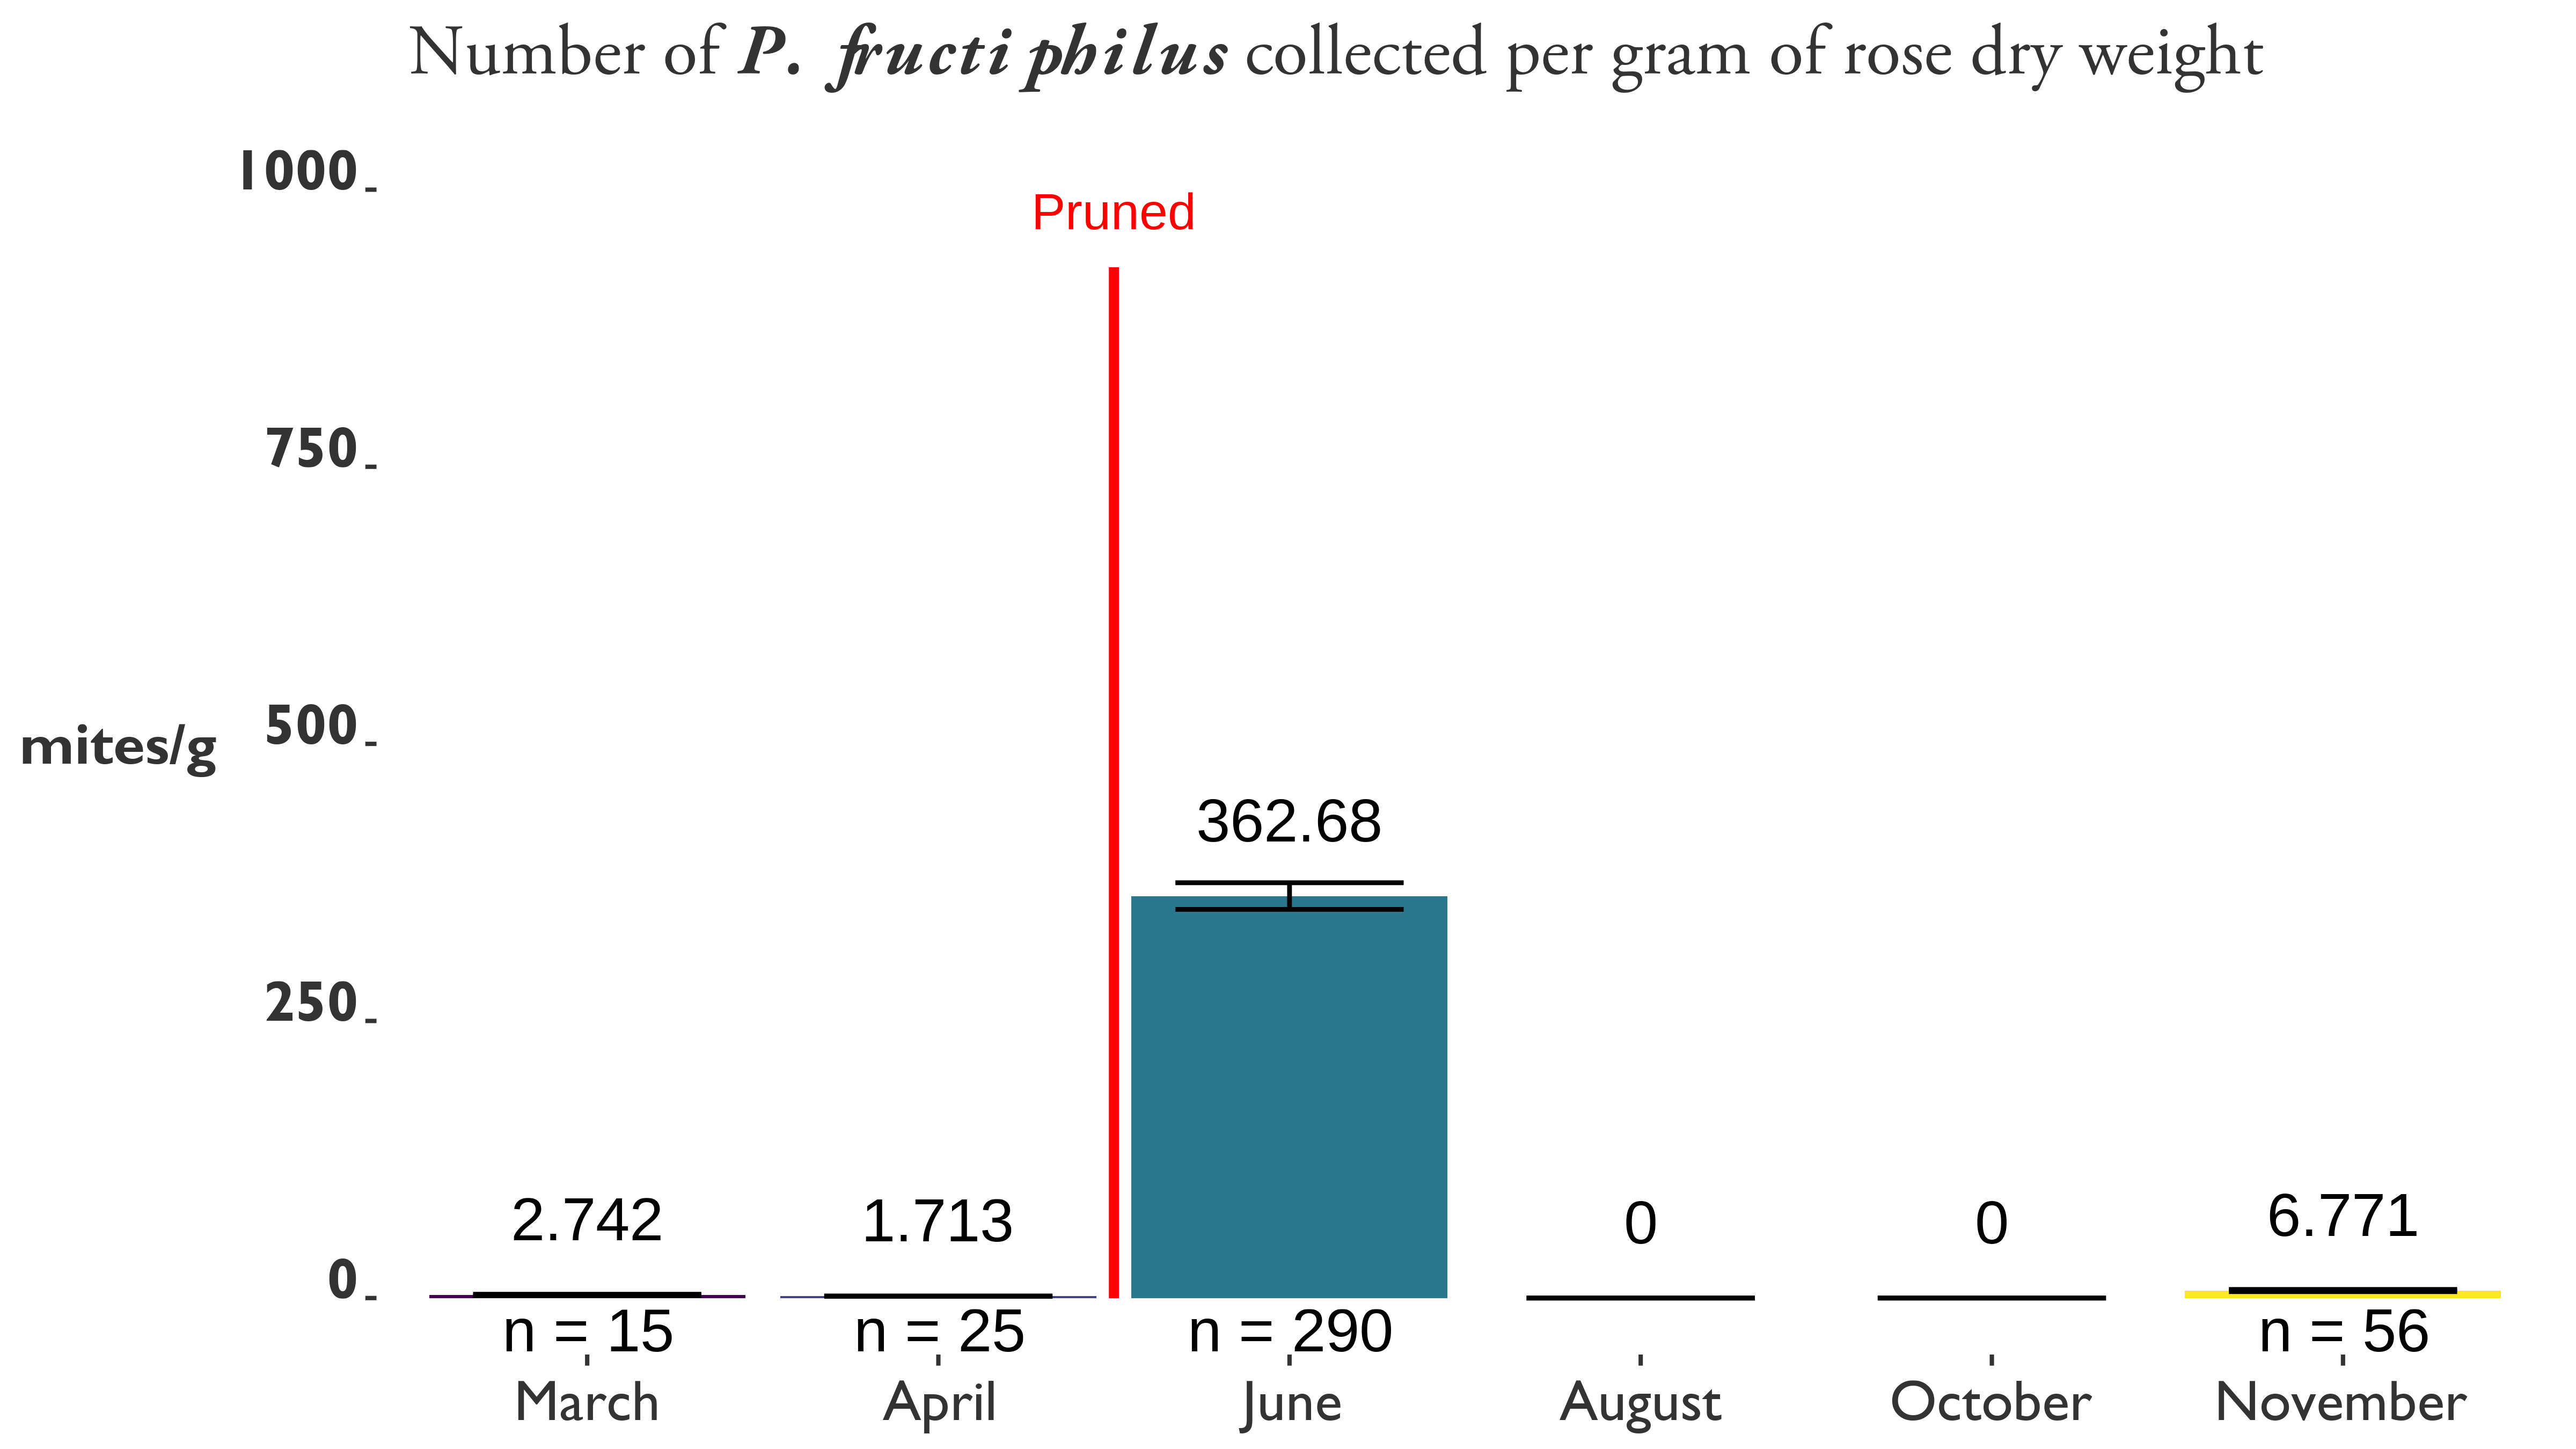
\includegraphics[width=1\linewidth]{figure/rrv_pheno_bargraph} 

}

\caption[Phenology of \textit{P. fructiphilus} mite populations on roses in Leon County, Florida]{Phenology of \textit{P. fructiphilus} mite populations on roses in Leon County, Florida 2020-2021. Roses were pruned back heavily on July 9, 2020.}\label{fig:pheno-graphs}
\end{figure}
\hypertarget{ipm-trials}{%
\subsection{IPM trials}\label{ipm-trials}}
\begin{figure}

{\centering 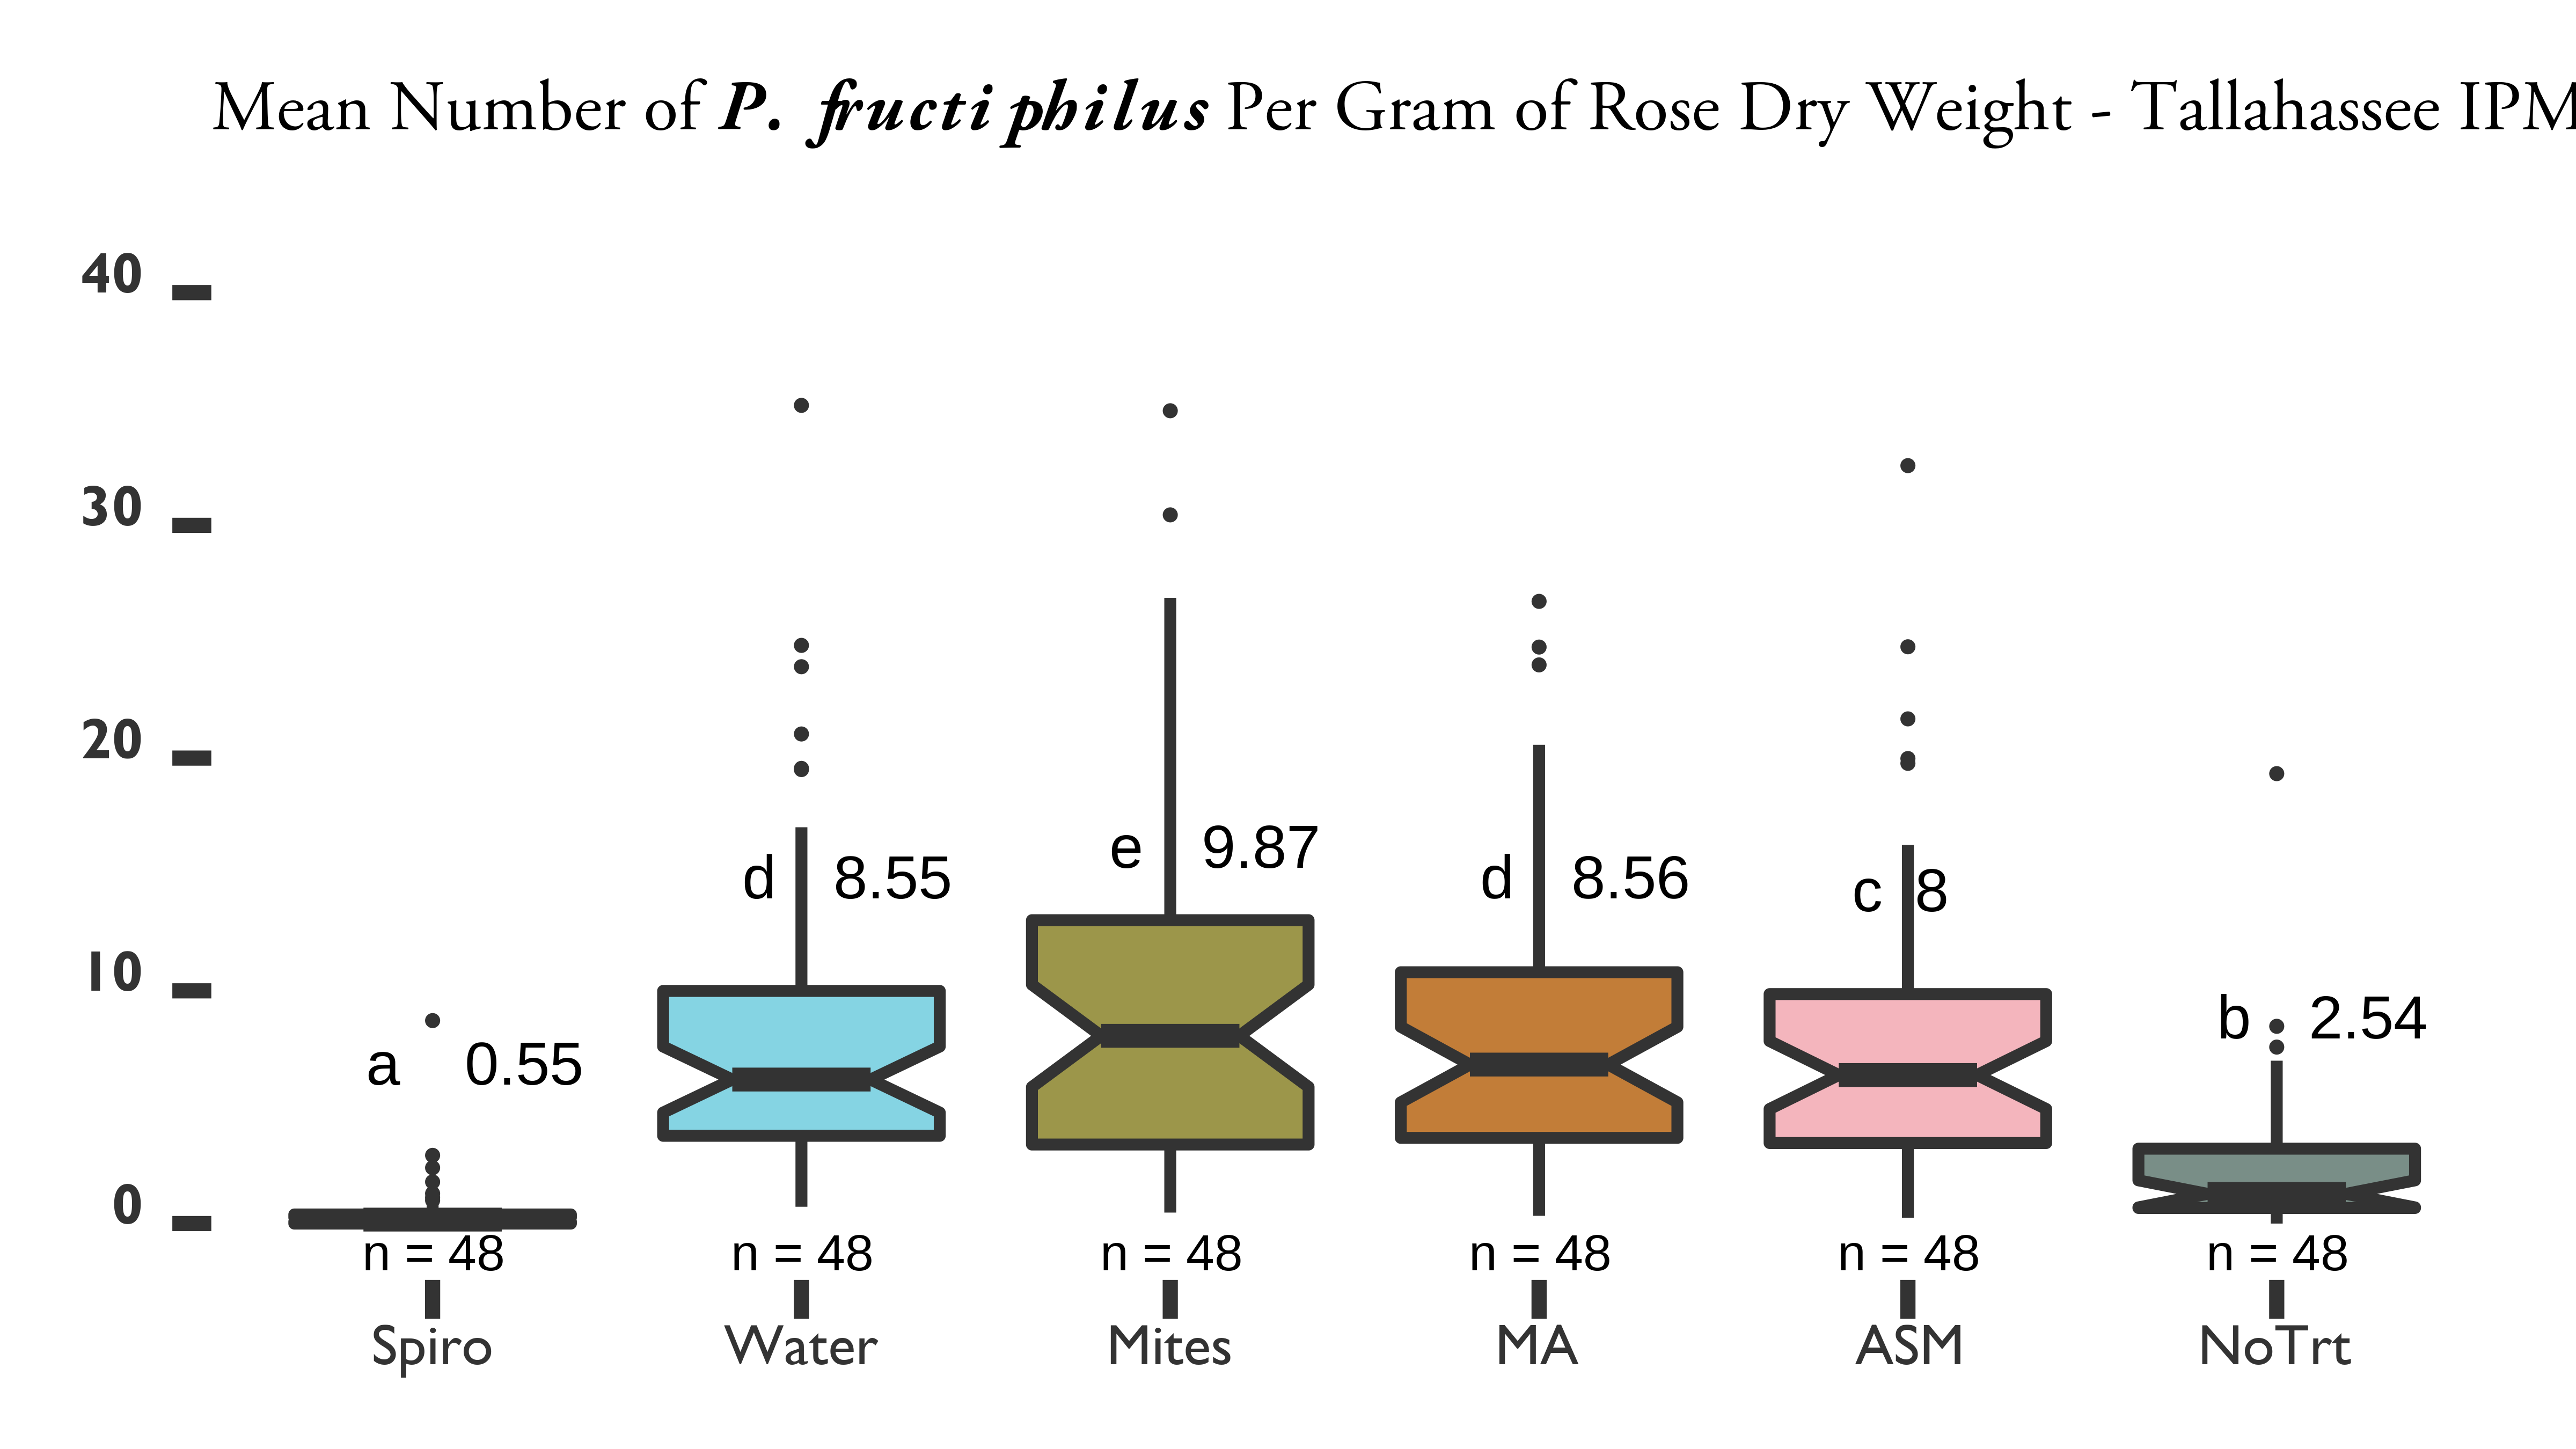
\includegraphics[width=1\linewidth]{figure/rrv_ipm_graph_erios_talla} 

}

\caption[IPM trials on Pink Double Knock Out® roses to control \textit{P. fructiphilus} in Tallahassee, FL with five treatments]{IPM trials on Pink Double Knock Out® roses to control \textit{P. fructiphilus} in Tallahassee, FL with five treatments. Statistical significance was determined using Tukey contrasts for multiple Comparisons of means. Groups which share letters are not statistically different from one another. $\alpha = 0.05$. Water = Water Control, ASM = Actigard50WG® (Syngenta, Greensboro, NC, USA) acibenzolar-S-methyl (ASM), Spiro = Kontos® Miticide Insecticide - Spirotetramat (Bayer Corporation, Whippany, New Jersey, USA), Mites = \textit{Amblyseius swirkii} predatory mite mini sachets on hooks (Ambly-S, Arbico Organics, Oro Valley, AZ, USA), MA = \textit{A. swirskii} + Actigard combined treatments. All products were applied at their label rates for 12 weeks. Flower cuttings were taken weekly to record the numbers of \textit{P. fructiphilus} and other herbivorous mites.}\label{fig:ipm-talla-erios}
\end{figure}
\begin{figure}

{\centering 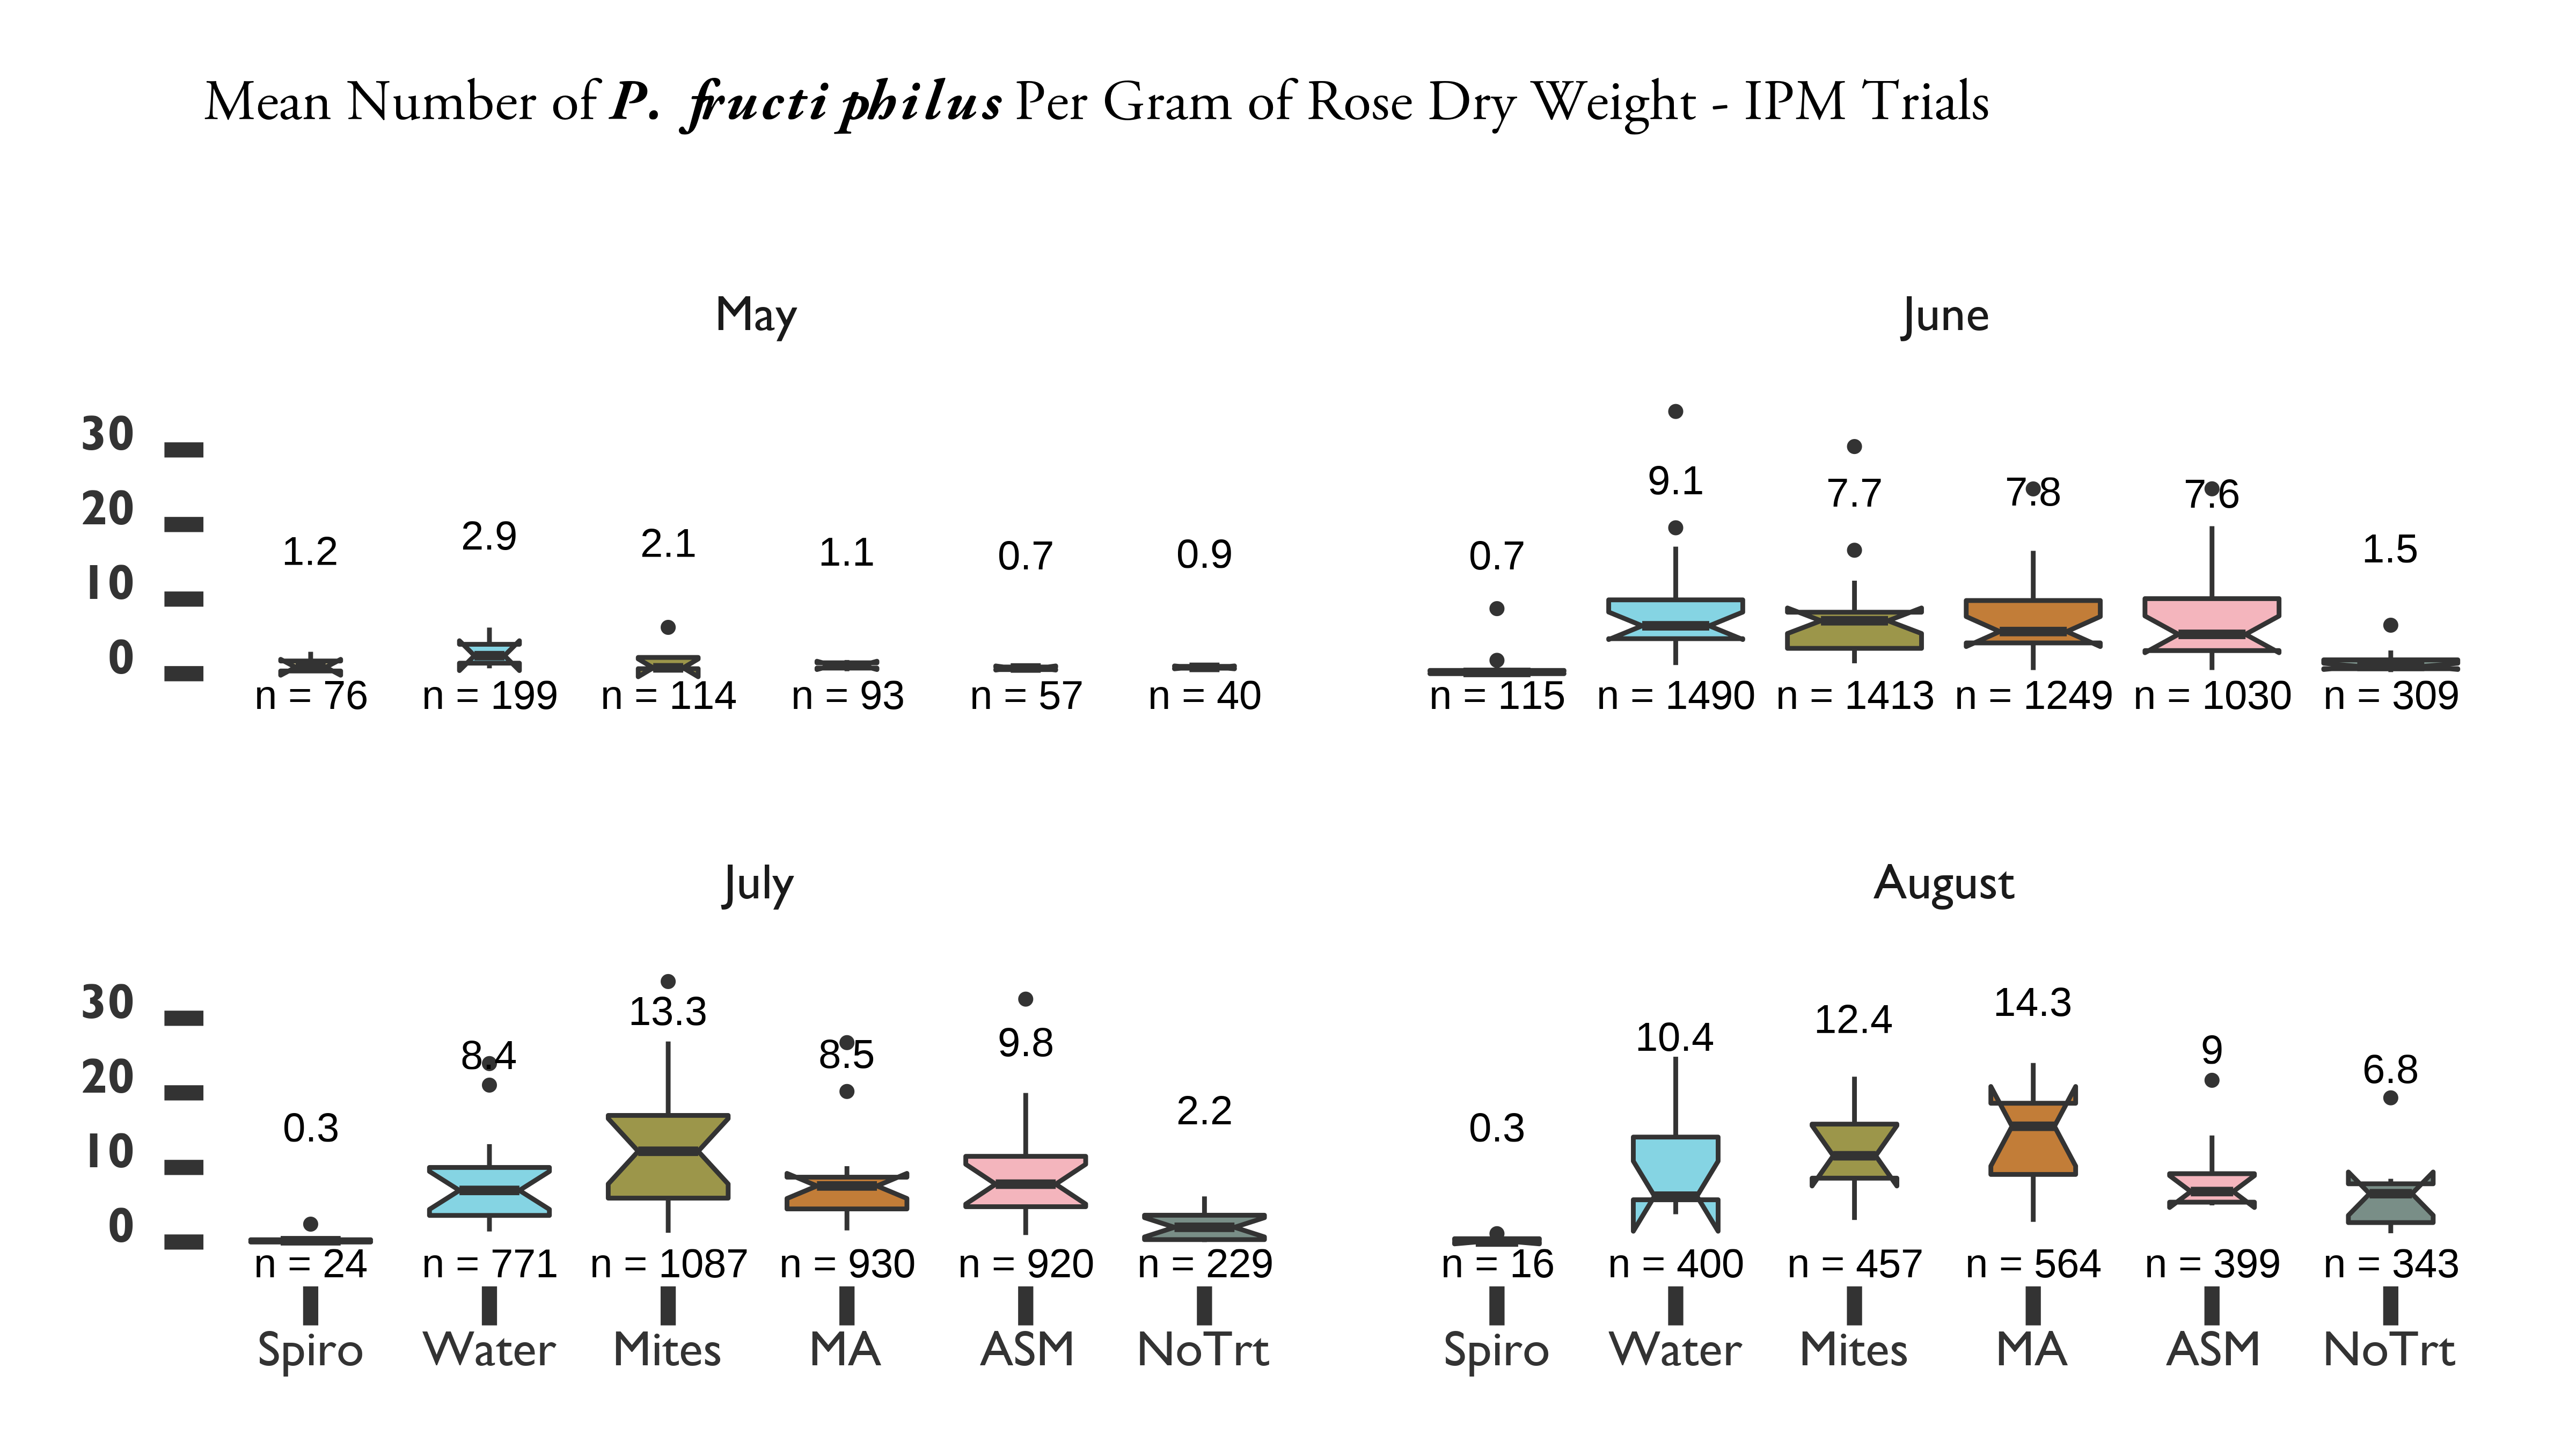
\includegraphics[width=1\linewidth]{figure/rrv_ipm_graph_erios_talla_month} 

}

\caption{IPM trials on Pink Double Knock Out® roses to control \textit{P. fructiphilus} in Tallahassee, FL with five treatments}\label{fig:ipm-talla-erios-month}
\end{figure}
\begin{figure}

{\centering 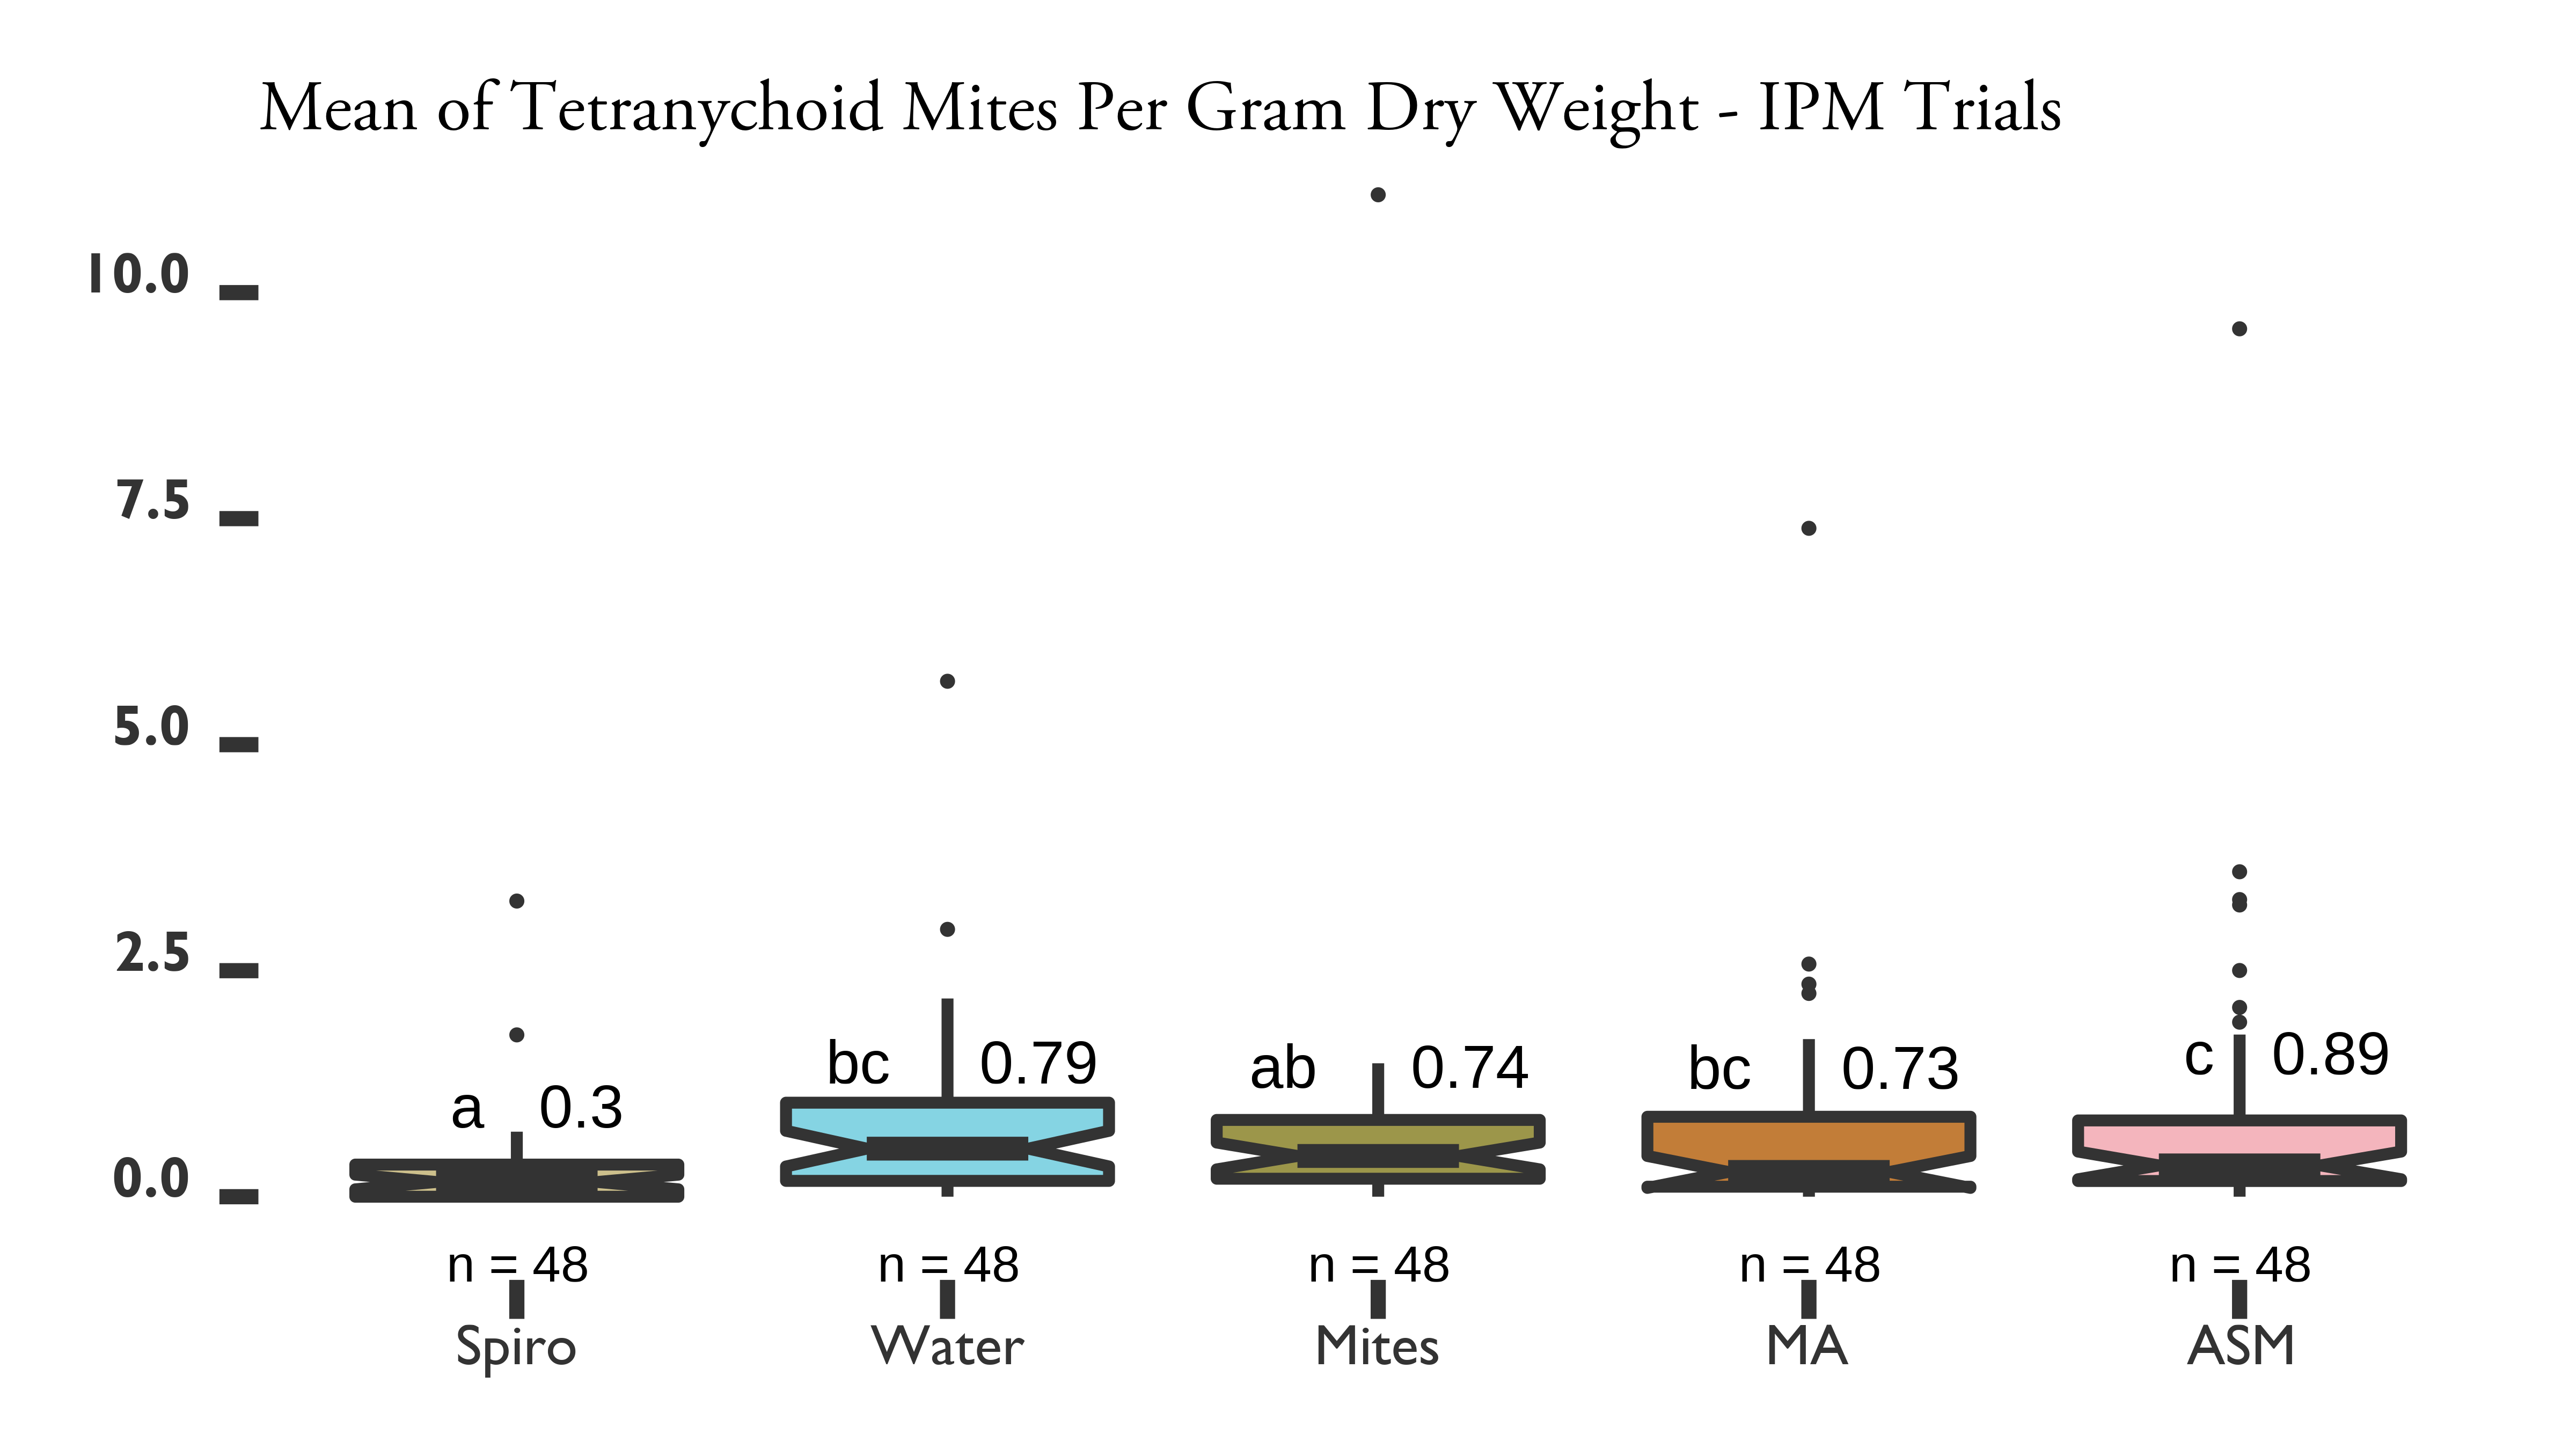
\includegraphics[width=1\linewidth]{figure/rrv_ipm_graph_tets_talla} 

}

\caption{IPM trials on Pink Double Knock Out® roses to control \textit{P. fructiphilus} in Tallahassee, FL with five treatments}\label{fig:ipm-talla-tets}
\end{figure}
\begin{figure}

{\centering 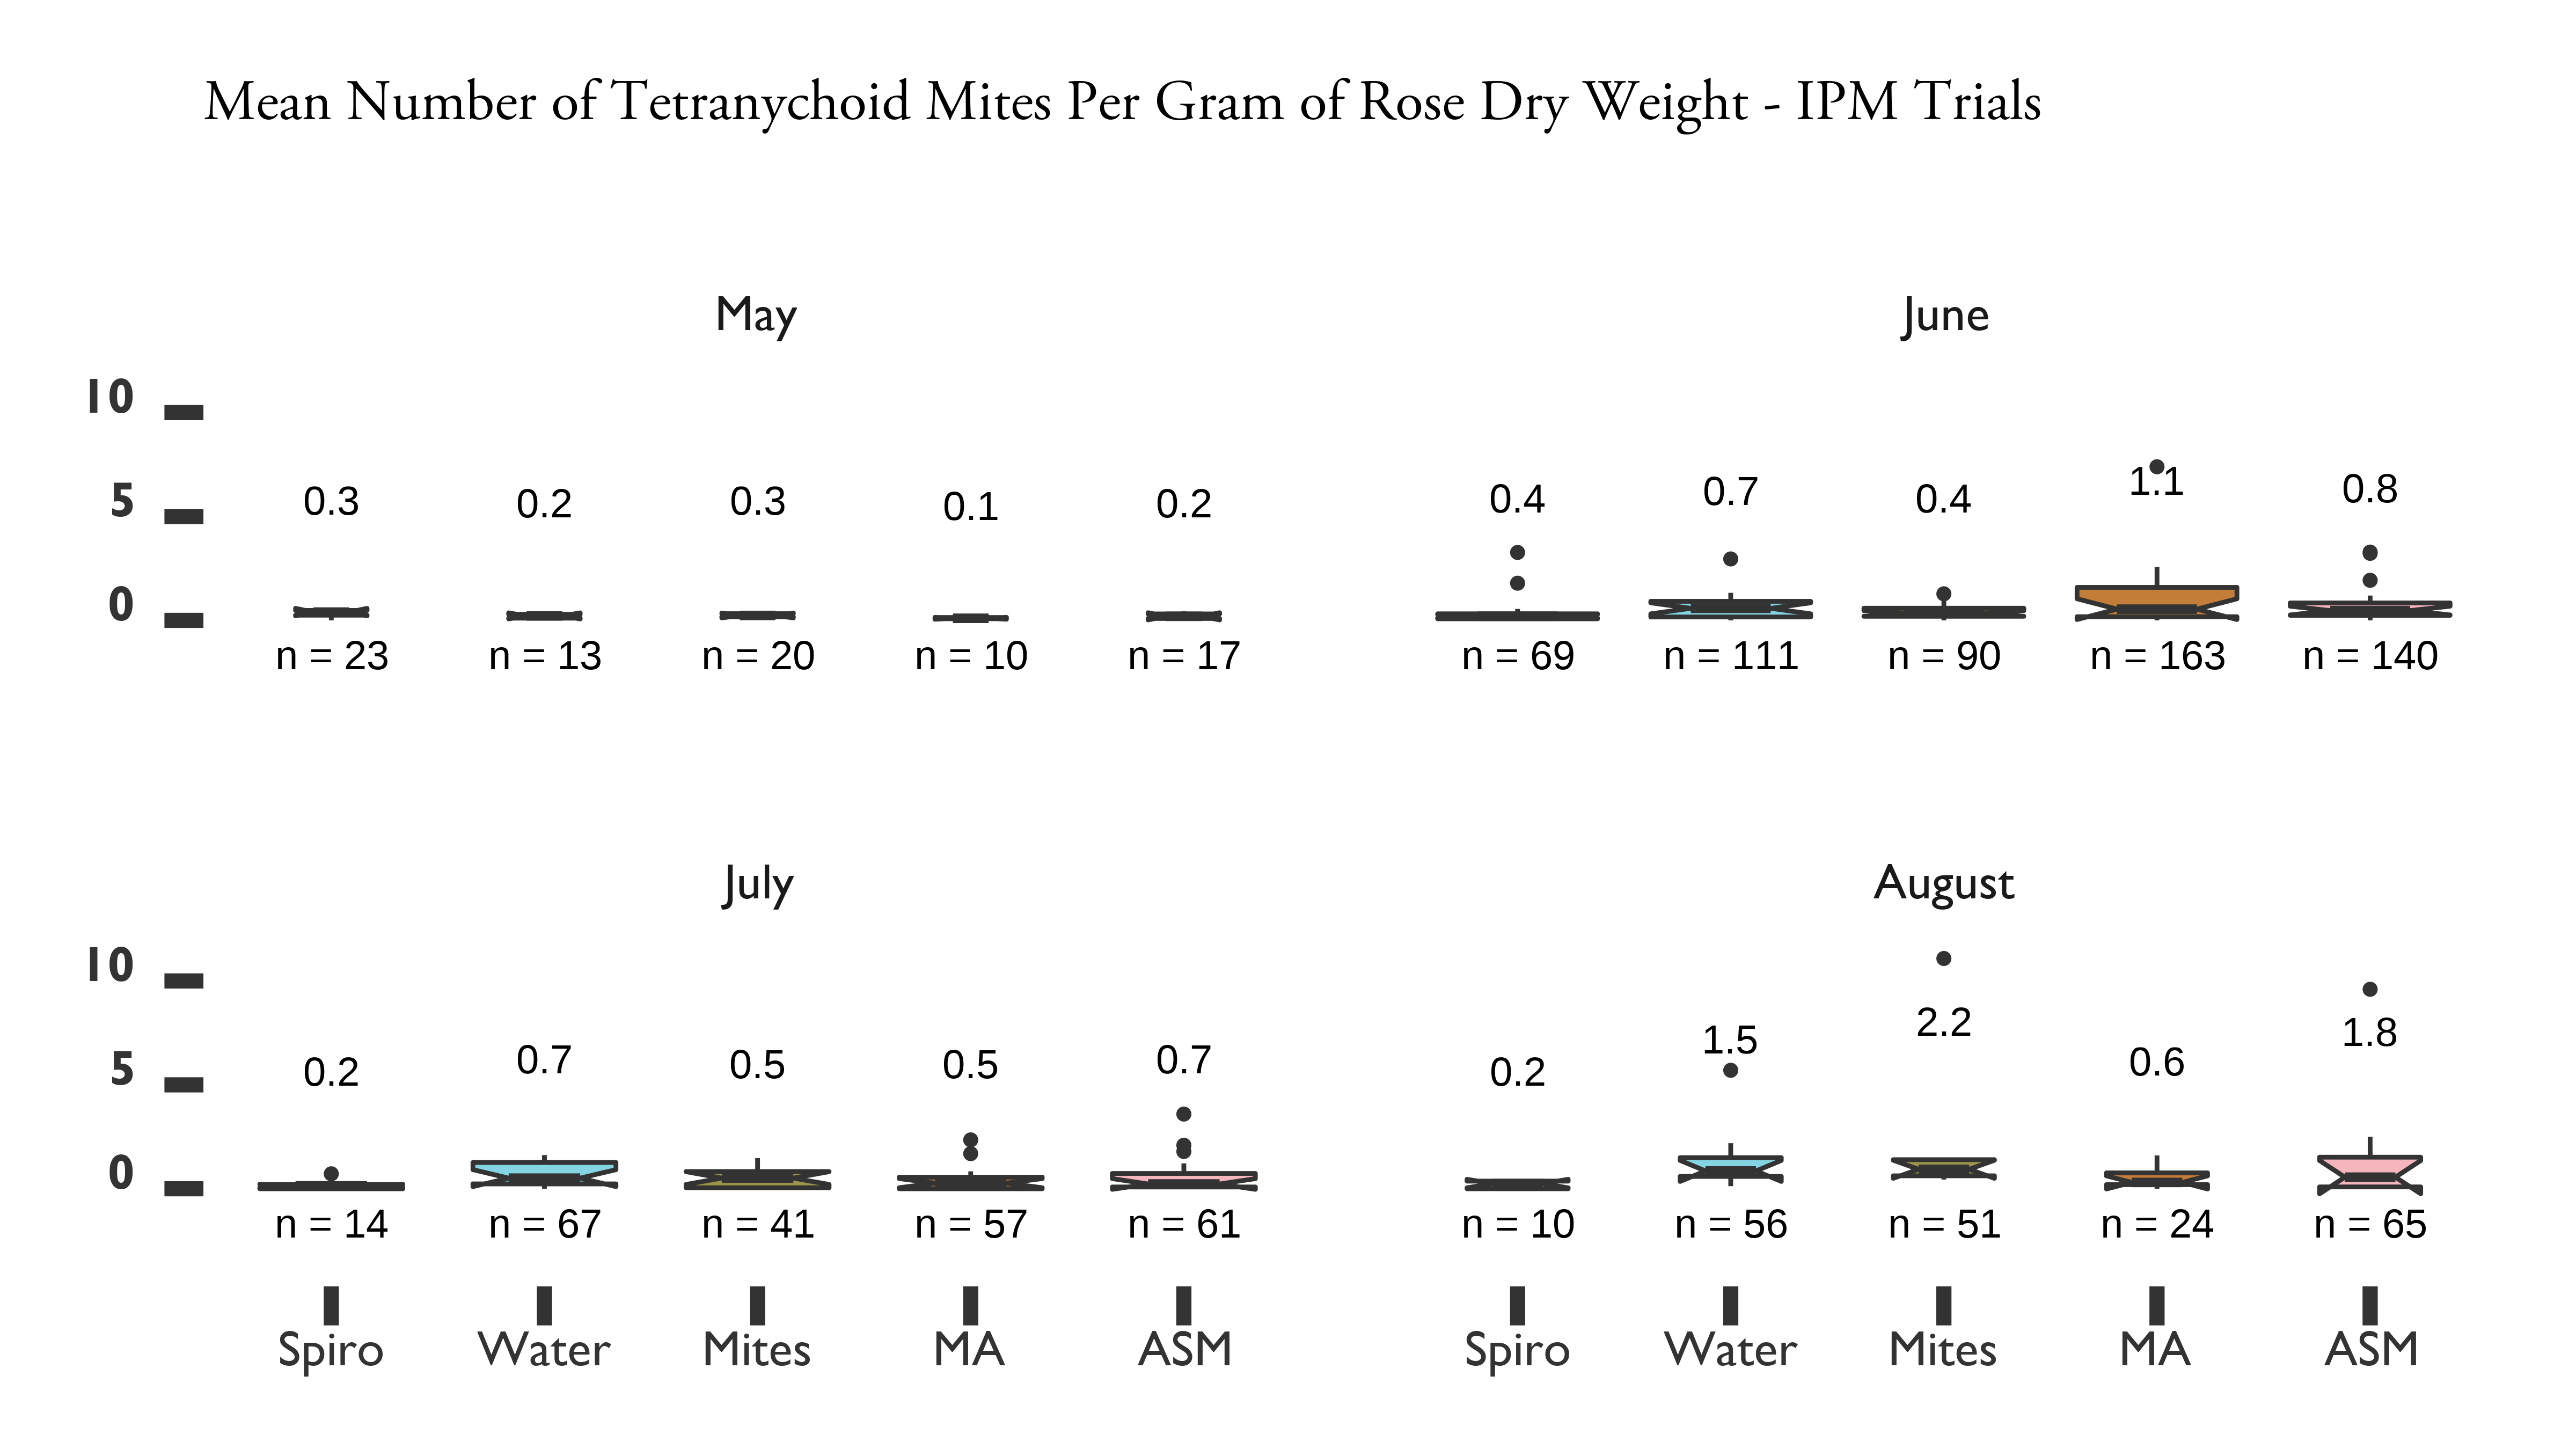
\includegraphics[width=1\linewidth]{figure/rrv_ipm_graph_tets_talla_month} 

}

\caption{IPM trials on Pink Double Knock Out® roses to control \textit{P. fructiphilus} in Tallahassee, FL with five treatments}\label{fig:ipm-talla-tets-month}
\end{figure}
\begin{figure}

{\centering 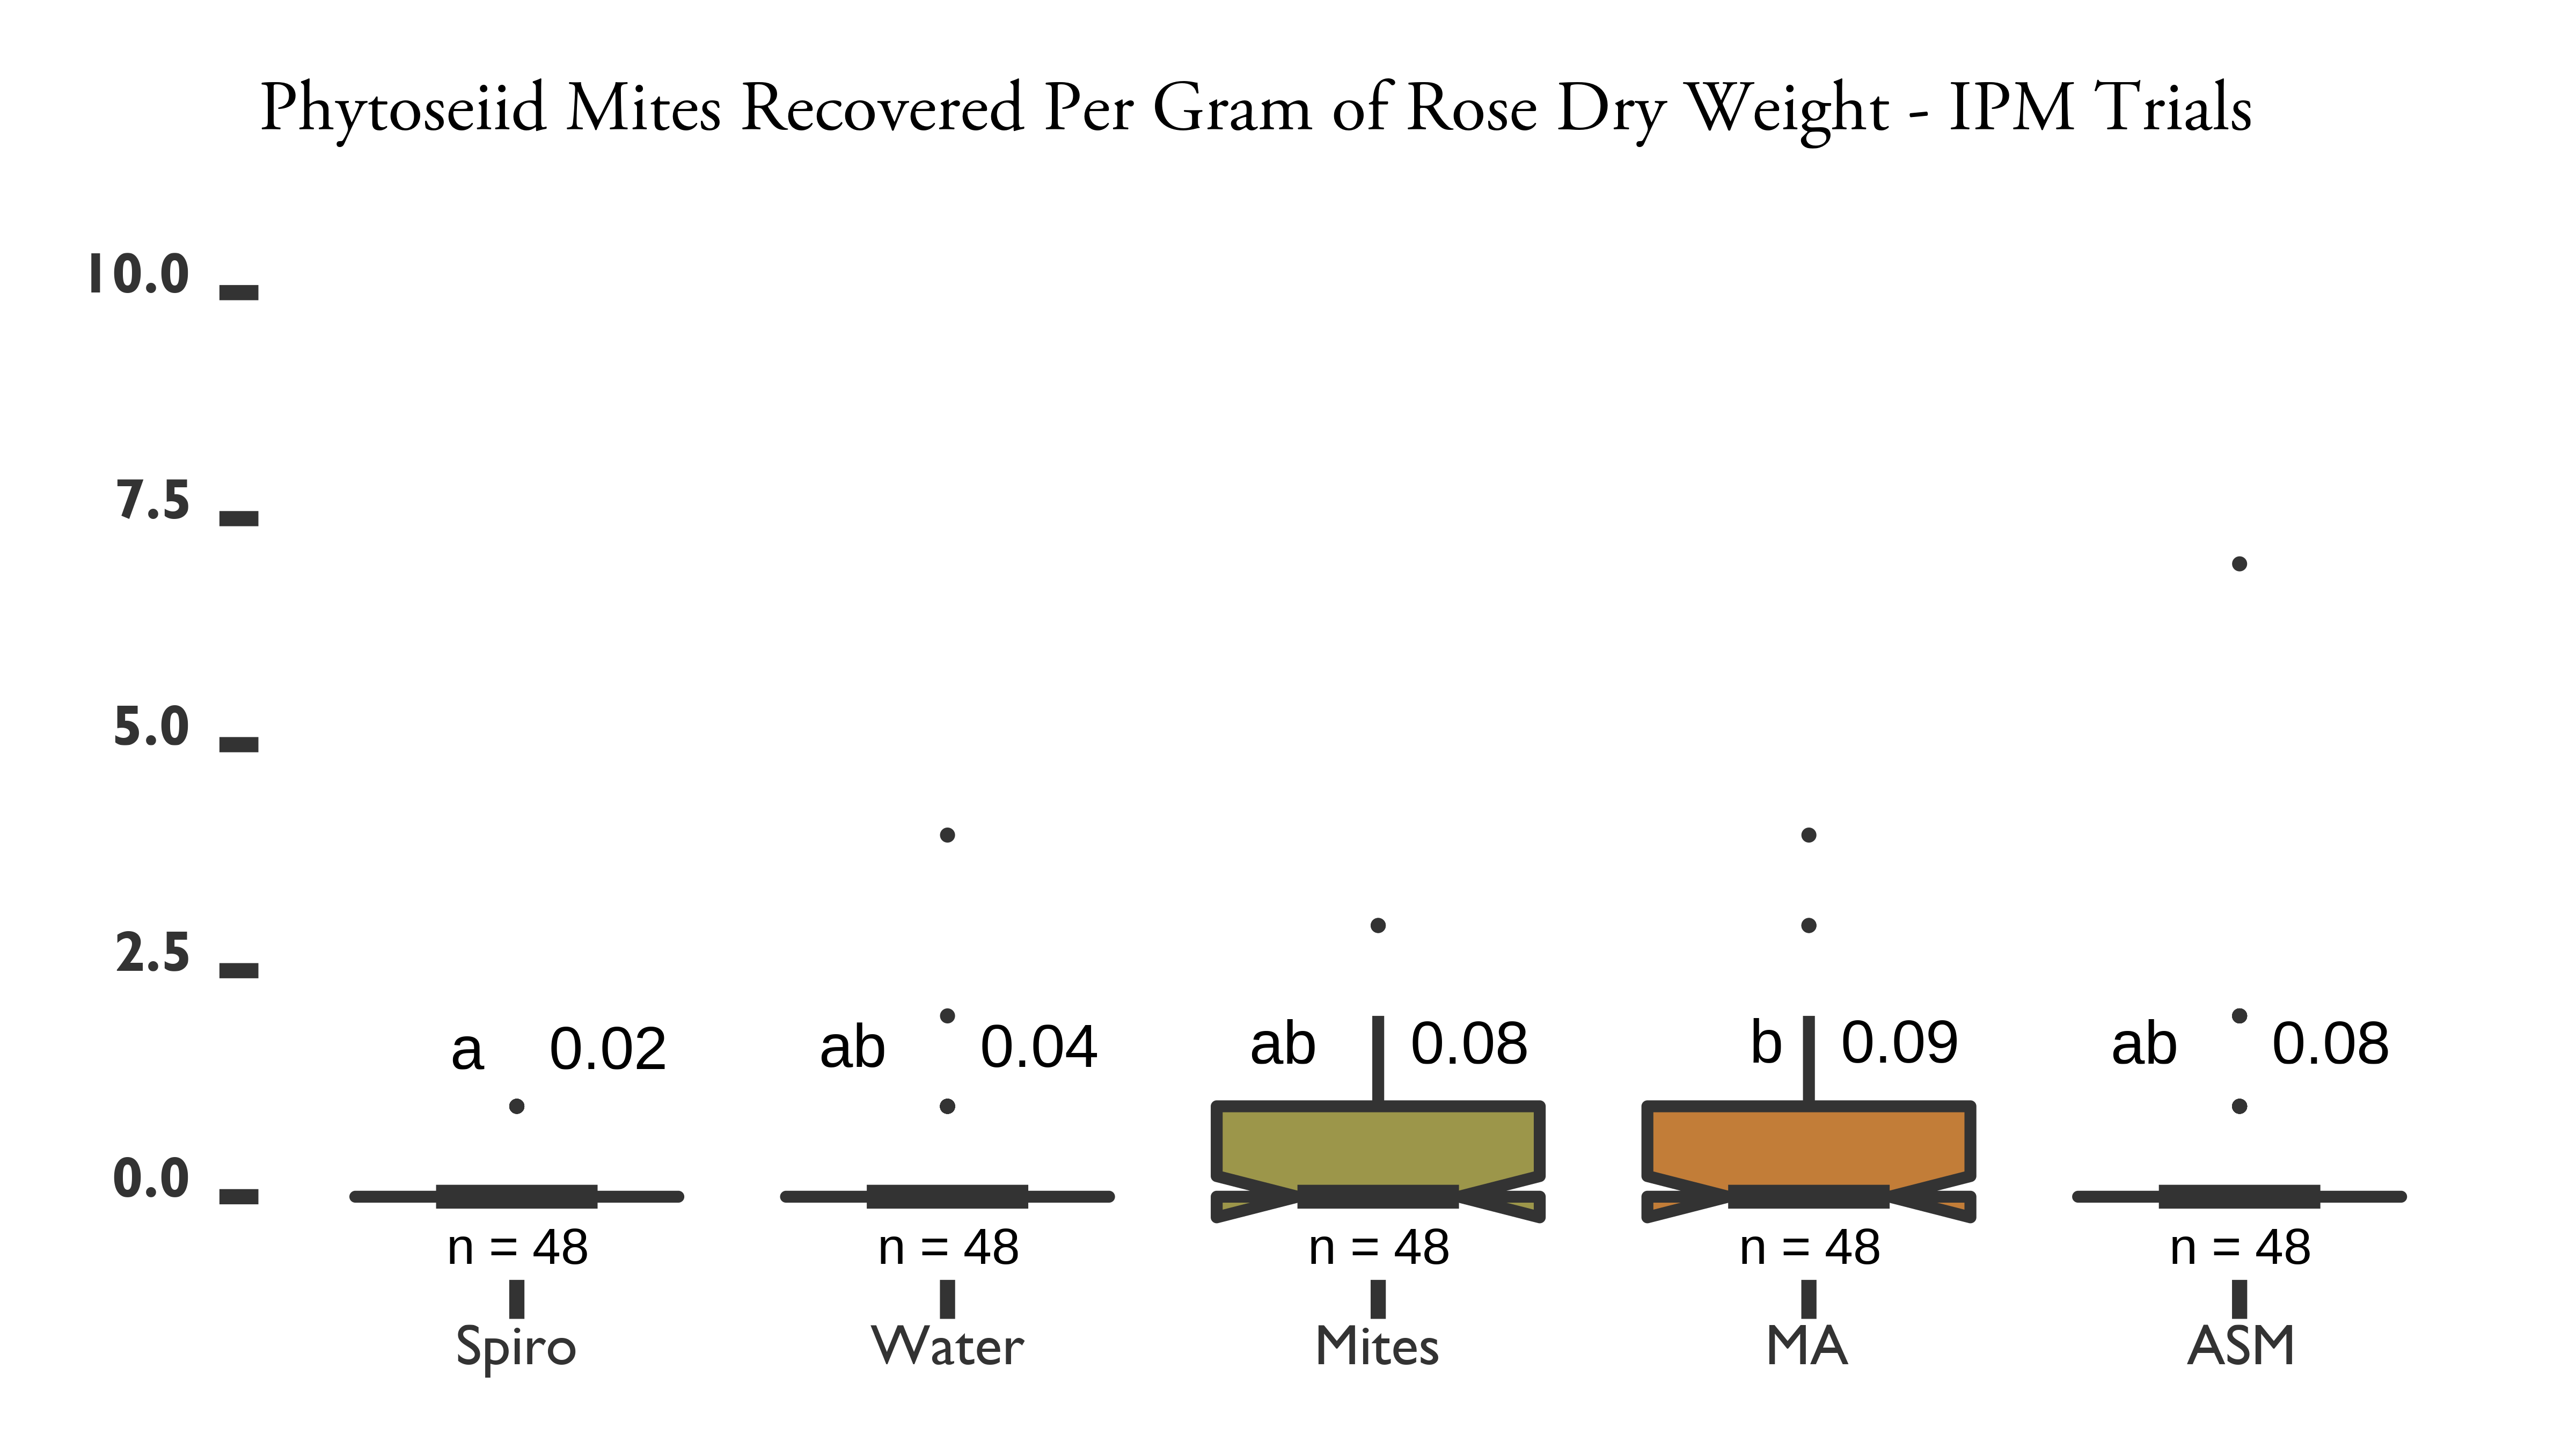
\includegraphics[width=1\linewidth]{figure/rrv_ipm_graph_preds_talla} 

}

\caption{IPM trials on Pink Double Knock Out® roses to control \textit{P. fructiphilus} in Tallahassee, FL with five treatments}\label{fig:ipm-talla-preds}
\end{figure}
\begin{figure}

{\centering 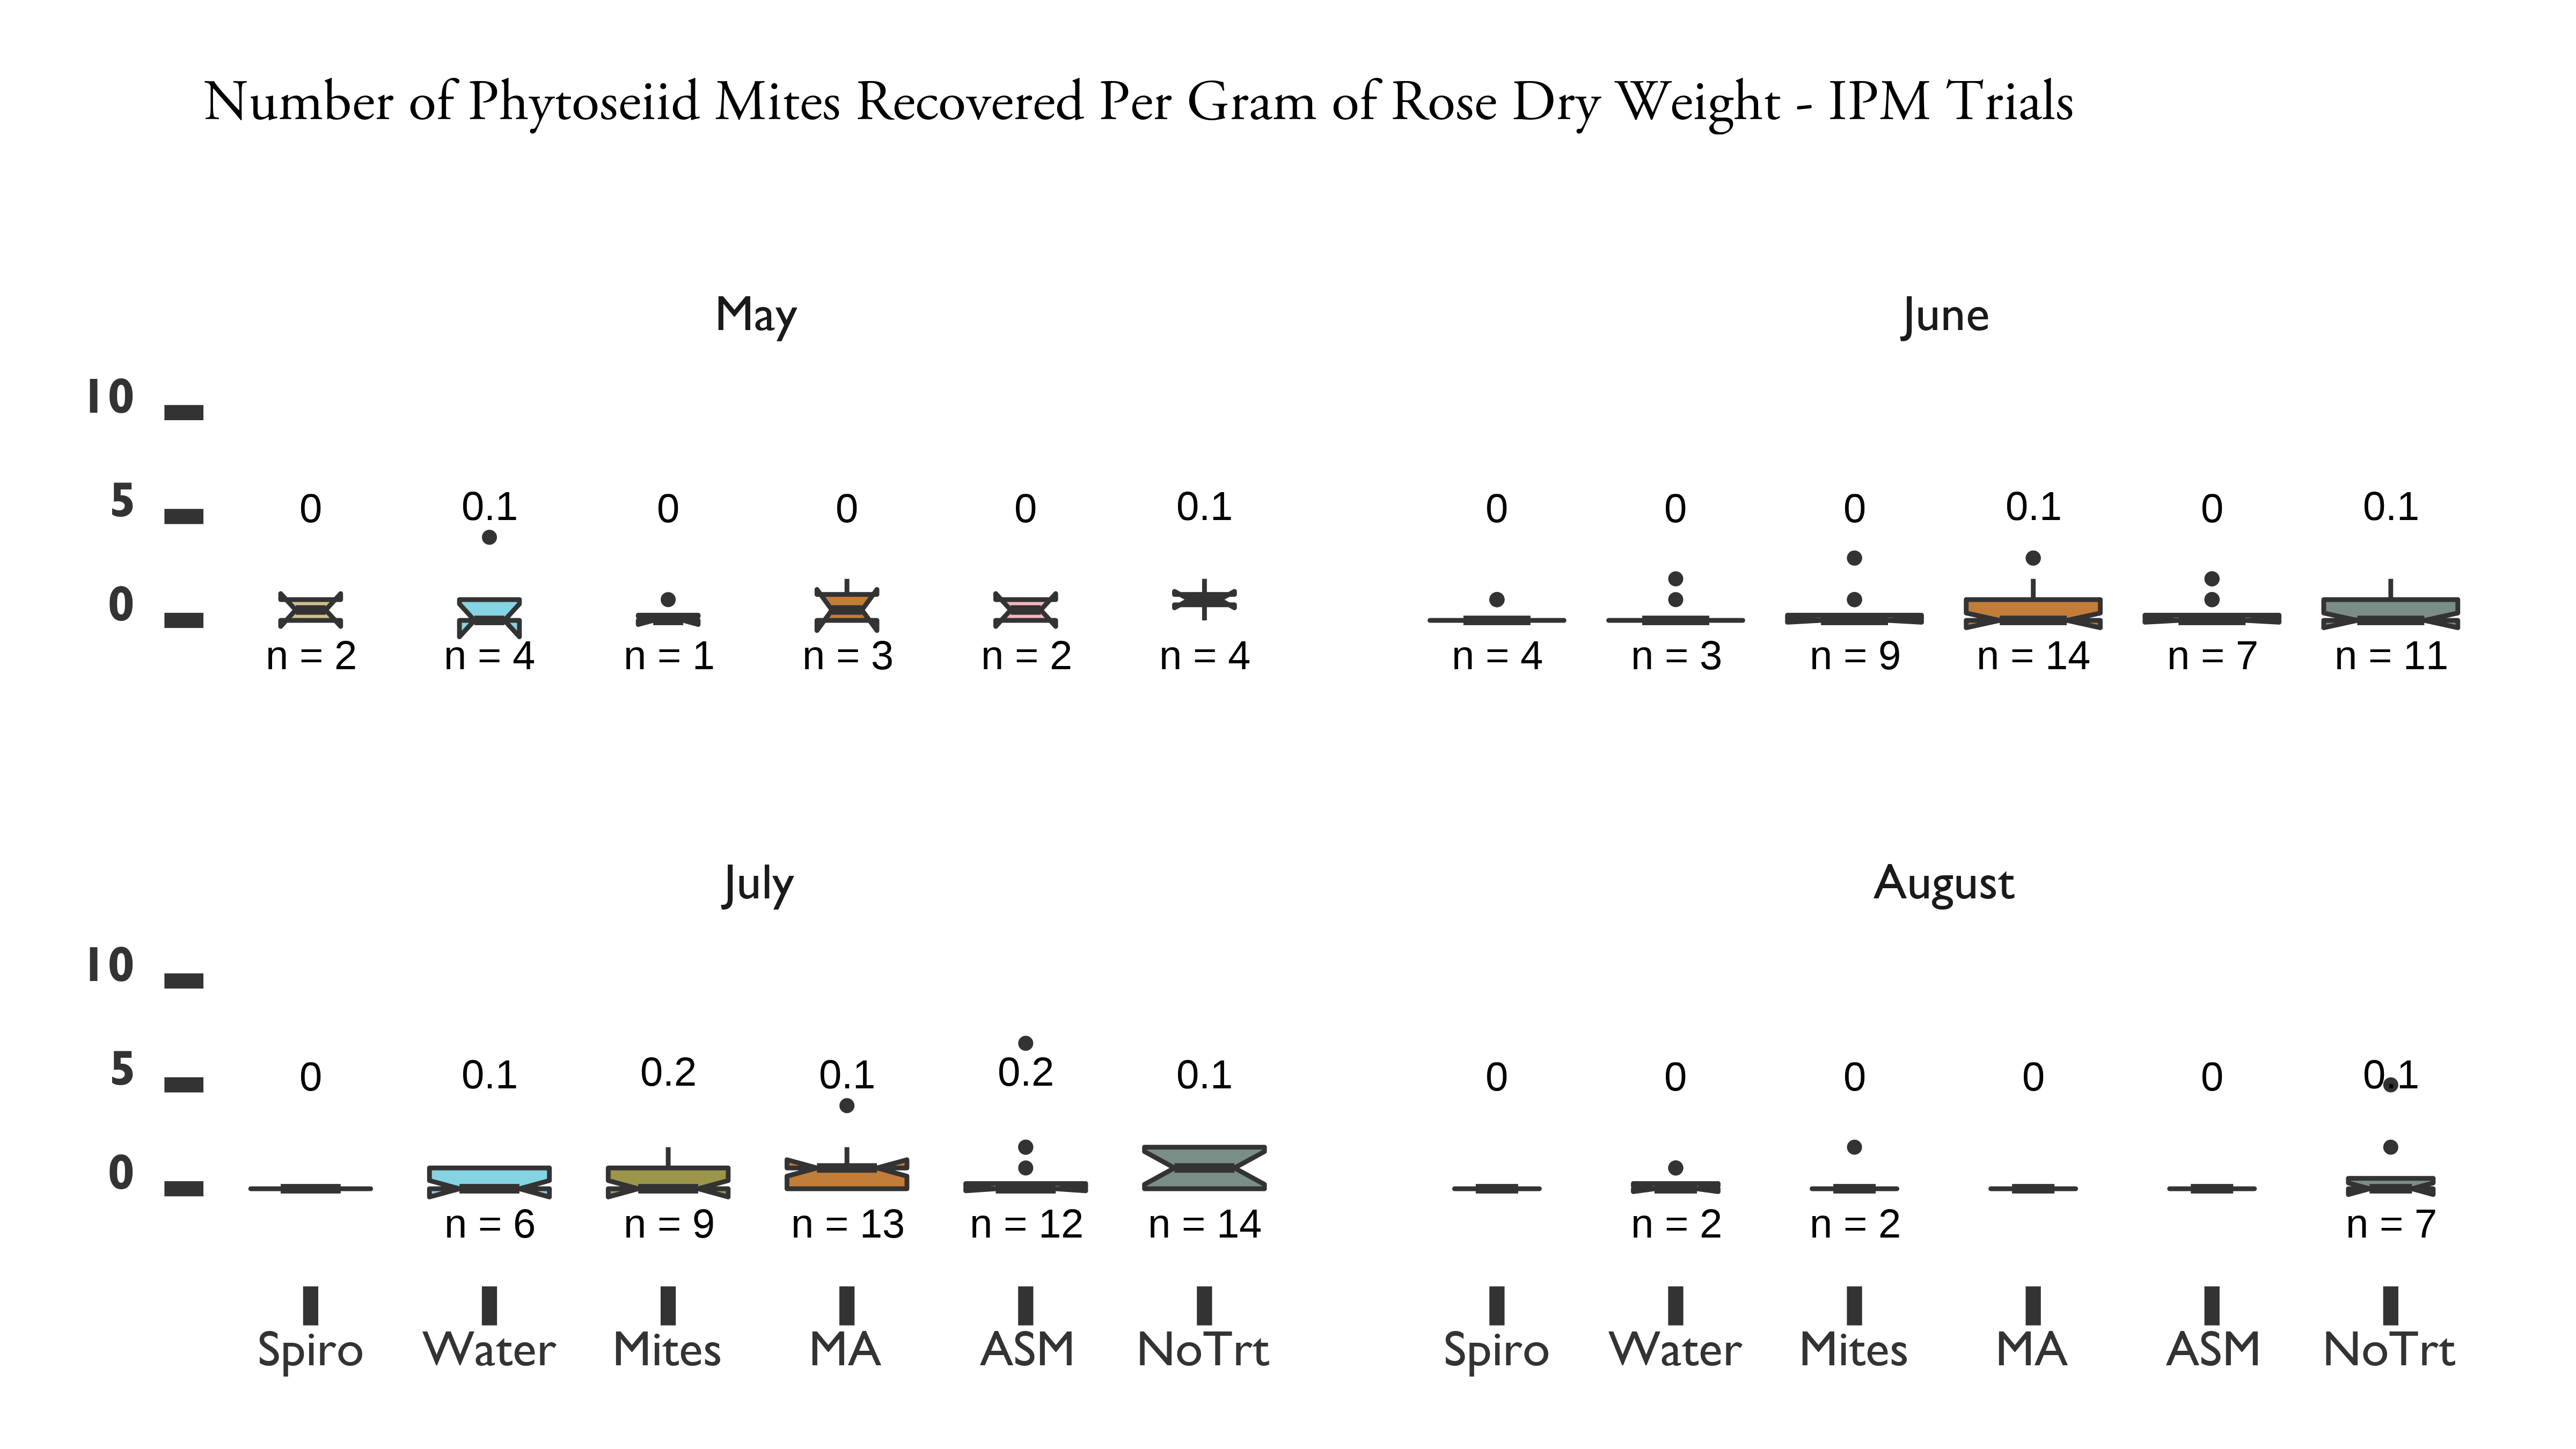
\includegraphics[width=1\linewidth]{figure/rrv_ipm_graph_preds_talla_month} 

}

\caption{IPM trials on Pink Double Knock Out® roses to control \textit{P. fructiphilus} in Tallahassee, FL with five treatments}\label{fig:ipm-talla-preds-month}
\end{figure}
\hypertarget{discussion-2}{%
\section{Discussion}\label{discussion-2}}

We had low recovery of \emph{P. fructiphilus} for the ASM and IPM trials in Georgia. This lead us to the phenology study, to ensure that there had been adequate establishment of \emph{P. fructiphilus} to create measurable effects. The phenology study was successful in measuring population fluctuations of eriophyid mites, and helped guarantee the presence of \emph{P. fructiphilus} before beginning the IPM trials in Tallahassee. Our results from the the IPM trials in Tallahassee suggest that spirotetramat were able to significantly reduce populations of \emph{P. fructiphilus}, an effect seen in all of the field trials conducted. Numbers of \emph{P. fructiphilius} on ASM-treated plants were were not significantly different than the control (see \emph{\ref{fig:ipm-talla-erios}}). \emph{A. swirskii} were recovered in smaller numbers than the other species of mites (see \emph{\ref{fig:ipm-talla-preds}}). Although we did not create barriers to prevent dispersal of \emph{A. swirskii}, these mites were most frequently recovered from the same plots where they were released. It is possible that we encountered few \emph{A. swirskii} because they dispersed to the point of leaving the rose plots (\protect\hyperlink{ref-Addesso2018}{Addesso et al. 2018}). This would make sense in the light of other studies: Buitenhuis et al. (\protect\hyperlink{ref-Buitenhuis2013}{2013}) noted the ability of \emph{A. swirskii} to move quickly on roses due to fewer trichomes, and recommended adjusting their release rates accordingly to maintain high populations on plants. \emph{A. swirskii} are not expected to disperse very far off of plants, but canopy connectivity between plants has been noted to increase their dispersal (\protect\hyperlink{ref-Buitenhuis2010}{Buitenhuis et al. 2010}). Ornamentals such as roses tend to be grown in separately spaced pots. Although the roses at our site were planted in the ground, the plots we tested did not have overlapping canopies, which may have reduced dispersal of \emph{A. swirskii} into other nearby roses. We anticipated seeing lower numbers of \emph{T. urticae} in plots where \emph{A. swirskii} had been released, but we did not see any correlations between releases of \emph{A. swirskii} on \emph{T. urticae}. Other studies have found \emph{A. swirskii} predation to be negatively correlated with trichome density (\protect\hyperlink{ref-Buitenhuis2013}{Buitenhuis et al. 2013}), suggesting that \emph{A. swirskii} are unlikely to feed on \emph{P. fructiphilus} hidden in the tightly appressed surfaces between rose sepals and petals. These areas also contain dense glandular trichomes, which tend to accumulate high quantities of VOCs (\protect\hyperlink{ref-Tissier2017}{Tissier et al. 2017}), defensive compounds (\protect\hyperlink{ref-Gerhold1984}{Gerhold et al. 1984}, \protect\hyperlink{ref-Ambrosio2008}{Ambrósio et al. 2008}, \protect\hyperlink{ref-Karabourniotis2019}{Karabourniotis et al. 2019}), or possibly entrap predators (\protect\hyperlink{ref-Nihoul1994}{Nihoul 1994}), benefits which erinea-producing eriophyids readily exploit to protect themselves (\protect\hyperlink{ref-Karioti2011}{Karioti et al. 2011}, \protect\hyperlink{ref-Karabourniotis2019}{Karabourniotis et al. 2019}). We did not see any correlations between \emph{A. swirskii} and \emph{P. fructiphilus}, as anticipated. Spirotetramat is known to less toxic to \emph{A. swirskii} (\protect\hyperlink{ref-Fernandez2017}{Fernández et al. 2017}), but no correlations emerged for \emph{A. swirskii} for either spirotetramat or ASM treatments. Some evidence has been given that slow release mite sachets which are sheltered and provided with felt patches (\protect\hyperlink{ref-Shimoda2017}{Shimoda et al. 2017}), and/or moisture in the form of water-absorbant sodium polyacrylate gels had better releases of predators (\protect\hyperlink{ref-Shimoda2018}{Shimoda et al. 2018}). It is also possible that there was an excess of pollen or other acceptable food sources which \emph{A. swirskii} preferred over the \emph{T. urticae} found in roses (\protect\hyperlink{ref-Leman2014}{Leman and Messelink 2014}), or competition with other predators encountered on the roses (\protect\hyperlink{ref-Doeker2021}{Döker et al. 2021}). A cursory examination of non-mite arthropods in rose samples revealed a number of unidentified species of thrips. \emph{A. swirskii} are known to feed on thrips, so there may be correlations between the predatory mites and the number of thrips in each treatment, but this requires a reexamination of the bycatch data. Another factor in our studies is the absence of RRV in our plots, which might otherwise mediate multitrophic interactions between the \emph{P. fructiphilus}, \emph{T. urticae} and \emph{A. swirskii} indirectly through induction of different plant defenses (\protect\hyperlink{ref-Belliure2010}{Belliure et al. 2010}). Some species of tetranychoids, including \emph{T. urticae}, are known to be able to suppress some plant defenses directly (\protect\hyperlink{ref-Sarmento2011}{Sarmento et al. 2011}, \protect\hyperlink{ref-Alba2014}{Alba et al. 2014}, \protect\hyperlink{ref-Arena2018}{Arena et al. 2018}, \protect\hyperlink{ref-Blaazer2018}{Blaazer et al. 2018}). This interference with plant defenses can interfere with the entire herbivore community (\protect\hyperlink{ref-Kant2015}{Kant et al. 2015}), including the eriophyoids feeding on the same plant (\protect\hyperlink{ref-Thaler2001}{Thaler et al. 2001}, \protect\hyperlink{ref-Glas2014}{Glas et al. 2014}), which should be examined for \emph{P. fructiphilus} control in future studies. Populations of \emph{P. fructiphilius} showed seasonal fluctuations in mite numbers, with highest populations achieved during June 2020 and July 2021. Rose pruning in July 2020 reduced the numbers of \emph{P, fructiphilus} collected for 3 months, populations began to recover that November. However, the number of \emph{P.fructiphilus} collected was not significantly different between the years 2020 and 2021 for the phenology trials. Mite numbers remained relatively lower during 2021 compared to the previous year. None of the mite-infested roses have shown symptoms of RRD to date. Tracking populations for longer periods of time with additional climatic data could be used to determine the best times to prune and apply chemistry to reduce mite numbers. The large reductions of \emph{P. fructiphilus} seen post pruning suggests its potential as a method of cultural mite control. The combination of pruning with acaricide treatments has been previously tested to control \emph{P. fructiphilus}, with limited success (\protect\hyperlink{ref-Windham2014}{Windham et al. 2014}), but these studies were conducted in areas of high pest pressure, with the presence of RRD. It is unlikely that acaricides or pruning are sufficient to prevent RRD infection: pruning does not remove the virus (\protect\hyperlink{ref-Bello2017}{Di Bello et al. 2017}), and the inoculation access period for transmission of RRD is surprisingly short, with mites able to transmit the virus within an hour of plant feeding (\protect\hyperlink{ref-Bello2017}{Di Bello et al. 2017}). Even so, the efficacy of combining pruning and acaricides has not been tested in areas with recent introductions of the mite without the virus. Combined management treatments may prove more effective in maintaining low populations of non-viruliferious \emph{P. fruciphilus}, and should be investigated for preventing the spread of the mite, rather than preventing the disease proper.

\hypertarget{brevipalpus-transmitted-orchid-fleck-dichorhavirus-infecting-three-new-ornamental-hosts-in-florida}{%
\chapter{\texorpdfstring{\emph{Brevipalpus}-TRANSMITTED \emph{Orchid fleck dichorhavirus} INFECTING THREE NEW ORNAMENTAL HOSTS IN FLORIDA}{Brevipalpus-TRANSMITTED Orchid fleck dichorhavirus INFECTING THREE NEW ORNAMENTAL HOSTS IN FLORIDA}}\label{brevipalpus-transmitted-orchid-fleck-dichorhavirus-infecting-three-new-ornamental-hosts-in-florida}}

Orchid fleck virus (OFV), is the type member for the genus \emph{Dichorhavirus}, family \emph{Rhabdoviridae}. The virus is a bacilliform, nuclear rhabdovirus composed of two segments of single-stranded, negative-sense RNA which infects plants (\protect\hyperlink{ref-Dietzgen2014}{Dietzgen et al. 2014}, \protect\hyperlink{ref-Walker2018}{Walker et al. 2018}, \protect\hyperlink{ref-Amarasinghe2019}{Amarasinghe et al. 2019}). Only Flat mites (Trombidiformes: Tenuipalpidae) from the genus \emph{Brevipalpus} are known to transmit dichorhaviruses (\protect\hyperlink{ref-Maeda1998}{Maeda 1998}). Plants infected with OFV exhibit chlorotic and necrotic flecks on their leaves(\protect\hyperlink{ref-Kubo2009}{Kubo et al. 2009b}, \protect\hyperlink{ref-Kubo2009a}{Kubo et al. 2009a}, \protect\hyperlink{ref-Dietzgen2018a}{Dietzgen et al. 2018b}). The virus was first described as infecting \emph{Cymbidium} orchids in Japan (\protect\hyperlink{ref-Doi1977}{Doi et al. 1977}). There have been reports of OFV and OFV-like rhabdoviruses infecting orchids in Asia, Africa, North America, South America, Europe, and Oceania. The prevalence of OFV and its mite vector is thought to be associated with the movement of infected orchids (\protect\hyperlink{ref-Dietzgen2018}{Dietzgen et al. 2018a}). More than fifty species of Orchidaceae (\protect\hyperlink{ref-Kitajima2010}{Kitajima et al. 2010}, \protect\hyperlink{ref-Peng2013}{Peng et al. 2013}) can naturally become infected with OFV, as well as some Asparagaceae (Nolinoidaea) (\protect\hyperlink{ref-Mei2016}{Mei et al. 2016}, \protect\hyperlink{ref-Dietzgen2018a}{Dietzgen et al. 2018b}), and Rutaceae, where infection causes citrus leprosis-like symptoms (\protect\hyperlink{ref-Roy2015}{Roy et al. 2015}, \protect\hyperlink{ref-Roy2020}{2020}, \protect\hyperlink{ref-Cook2019}{Cook et al. 2019}, \protect\hyperlink{ref-Velarde2021}{Olmedo-Velarde et al. 2021}). Mechanical transmission of OFV is possible under laboratory conditions to the plant families Chenopodiaceae, Aizoaceae, Fabaceae, and Solanaceae (\protect\hyperlink{ref-Chang1976}{Chang et al. 1976}, \protect\hyperlink{ref-Kondo2003}{Kondo et al. 2003}, \protect\hyperlink{ref-Peng2013}{Peng et al. 2013}), and a natural infection of OFV was recently reported infecting common hollyhock (Malvaceae, \emph{Alcea rosea} L.) in South Africa (\protect\hyperlink{ref-Read2021}{Read et al. 2021}).

\hypertarget{virus-detection}{%
\section{Virus Detection}\label{virus-detection}}

During June 2020, chlorotic flecks and ringspot patterns of unknown etiology were observed on Giant Lilyturf \emph{Liriope} spp., cv. `Gigantea' in a landscape of Leon County, Florida (\ref{fig:fig-1}). \emph{Liriope} belong to a group of plants in the family Asparagaceae, subfamily Nolinoidaea, comprised of grass-like monocotyledonous liliod plants native to southeastern Asia (\protect\hyperlink{ref-Chase2009}{Chase et al. 2009}, \protect\hyperlink{ref-Meng2021}{Meng et al. 2021}). \emph{Liriope} and the closely related \emph{Ophiopogon} (Asparagaceae: Nolinoidaea) are considered the most important ground cover plant in the southeastern United States (\protect\hyperlink{ref-Mcharo2003}{Mcharo et al. 2003}). Viral infections of suspected leaf samples were initially tested at the Plant Disease Diagnostic Clinic at the North Florida Research and Education Center (NFREC) in Quincy, FL. All the samples were tested with one step conventional RT-PCR, and were found negative for begomovirus, carlavirus, potyvirus, tospovirus, cucumber mosaic virus and tobacco mosaic virus. As initial diagnostics were inconclusive, samples were taken of putatively infected plants with ringspot symptoms during July and August of 2020. Leaves were taken from \emph{Liriope} and \emph{Ophiopogon} spp., as well as the \emph{Aspidistra elatior} Blume (Asparagaceae: Nolinoidaea), nearby, which appeared sickly and chlorotic (\ref{fig:fig-2}). Plant materials were sent to the Florida Department of Agriculture and Consumer Services (FDACS) for identification. The FDACS determined that the pathogen was OFV using previously published primers and methods to conduct RT-PCR and Sanger sequencing (\protect\hyperlink{ref-Kubo2009}{Kubo et al. 2009b}, \protect\hyperlink{ref-Kubo2009a}{Kubo et al. 2009a}, \protect\hyperlink{ref-RamosGonzalez2015}{Ramos-González et al. 2015}).
The identity of the virus was verified as OFV Orchid strain 1, (OFV-Orc1), following the methods described in Kondo et al. (\protect\hyperlink{ref-Kondo2017}{2017}). Nucleotide sequencing shared 98\% nucleotide identity with the OFV-isolates So (Accession No.~AB244418) and Br (Accession No.~MK522807), which belong to orchid subgroup I (\protect\hyperlink{ref-Kondo2006}{Kondo et al. 2006}, \protect\hyperlink{ref-Kondo2017}{2017}). These samples from FDACS were subsequently retested by the USDA-APHIS-PPQ S\&T Beltsville laboratory, in conjunction with tests of fresh samples from both Alachua and Leon counties. The USDA used RT-PCR, RT-qPCR, and High Throughput Sequencing (HTS) to reconfirm the presence of OFV. Conventional RT-PCR with Generic R2-Dicho-GF and R2-Dicho-GR primers amplified \textasciitilde800 nt amplicons of the L-gene (RNA2) (\protect\hyperlink{ref-Roy2020}{Roy et al. 2020}), to detect both OFV-Orc1 and OFV-Orc2 in \emph{O. intermedius} and \emph{A. elatior} from Leon County (\protect\hyperlink{ref-Kondo2017}{Kondo et al. 2017}) (GenBank Accession Numbers: MZ852004, MZ852005 MZ852006, and MZ852007). 99\% nucleotide sequence identity is shared between OFV-Orc1 and OFV-Orc2 for the RNA2 genome, whereas 90\% sequence identity was found between these two reassortment strains. The presence of OFV-Orc1 and OFV-Orc2 in Leon and Alachua counties was reaffirmed with HTS data (\ref{tab:tab-1}): Analysis of HTS data from Leon County found that the symptomatic \emph{L. muscari} were coinfected with both OFV-Orc1 and OFV-Orc2, while the symptomatic \emph{A. elatior} were solely infected with OFV-Orc1. Sequence data of symptomatic \emph{L. muscari} from Alachua County revealed infections with OFV-Orc2 (GenBank Accession MZ852006). After the initial identification by FDACS of OFV-Orc, mite samples were collected from symptomatic Asparagaceae in Leon County. Most mites collected were Tenuipalpid mites (flat mites or false spider mites), a pest of ornamental plants, some of which are known to act as vectors for plant viruses (\protect\hyperlink{ref-Childers2003}{Childers et al. 2003b}, \protect\hyperlink{ref-Childers2011}{Childers and Rodrigues 2011}).
\begin{figure}

{\centering \includegraphics[width=1\linewidth]{thesis_files/figure-latex/fig-1-1} 

}

\caption[Variety of symptoms seen on \textit{Liriope} spp. infected with Orchid Fleck Virus]{Variety of symptoms seen on \textit{Liriope} spp. infected with Orchid Fleck Virus (OFV): (a) symptoms on \textit{Liriope muscari} cv. 'Gigantea' (b-c) Details of symptoms on \textit{L. muscari} cv. `Gigantea` (d) rust colored spots on \textit{Ophiopogon intermedius}}\label{fig:fig-1}
\end{figure}
\begin{figure}

{\centering \includegraphics[width=1\linewidth]{thesis_files/figure-latex/fig-2-1} 

}

\caption[Symptoms seen on \textit{Aspidistra elatior} infected with OFV]{Symptoms seen on \textit{Aspidistra elatior} infected with OFV: (a) Detail of leaf chlorosis (b) Chlorosis appears similar to sun damage (c-d) Chlorotic flecks may indicate early symptoms of OFV}\label{fig:fig-2}
\end{figure}
\begin{table}[H]

\caption{\label{tab:tab-1}List of Asparagaceae (Nolinoidaea) species infected with OFV, collected from the landscape of northern Florida.}
\centering
\resizebox{\linewidth}{!}{
\begin{threeparttable}
\begin{tabular}[t]{llll}
\toprule
Scientific Name & Common Names & County & Strains Detected\\
\midrule
\cellcolor{gray!6}{\textit{Liriope muscari} cv. ‘Gigantea’\textsuperscript{*} (Decaisne) Bailey} & \cellcolor{gray!6}{Lilyturf, Orchardgrass, Monkeygrass} & \cellcolor{gray!6}{Leon \& Alachua} & \cellcolor{gray!6}{OFV-Orc1 \& OFV-Orc2}\\
\textit{Ophiopogon intermedius}\textsuperscript{\dag} Don & Aztec Grass, Argenteomarginatus & Leon & OFV-Orc1 \& OFV-Orc2\\
\cellcolor{gray!6}{\textit{Aspidistra elatior} Blume} & \cellcolor{gray!6}{Cast Iron Plant, Bar-room Plant} & \cellcolor{gray!6}{Leon} & \cellcolor{gray!6}{OFV-Orc1 \& OFV-Orc2}\\
\bottomrule
\end{tabular}
\begin{tablenotes}
\item \textit{Note: } 
\item Both OFV-Orc1 and OFV-Orc2 were detected in each species tested, many plants were coinfected with both strains'.
\item[*] \textit{L. muscari} cv. ‘Gigantea’ has been traditionally classified as \textit{L. gigantea} Hume by Broussard 2007 and Fantz et al. 2015, although this distinction has been challenged by Wang et al. 2014 and Masiero et al. 2020.
\item[\dag] \textit{O. intermedius} is sometimes misclassified as \textit{L. muscari} ‘Variegated Evergreen Giant’ or ‘Grandiflora White’ (Fantz 2008b, 2009).
\end{tablenotes}
\end{threeparttable}}
\end{table}
\hypertarget{a-comment-on-the-status-of-brevipalpus-in-florida}{%
\section{\texorpdfstring{A Comment on the Status of \emph{Brevipalpus} in Florida}{A Comment on the Status of Brevipalpus in Florida}}\label{a-comment-on-the-status-of-brevipalpus-in-florida}}

Mite taxonomy is complicated by cryptic species complexes which occur in many plant-feeding groups of the Acari (\protect\hyperlink{ref-Umina1999}{Umina and Hoffmann 1999}, \protect\hyperlink{ref-Skoracka2010}{Skoracka and Dabert 2010}, \protect\hyperlink{ref-Arthur2011}{Arthur et al. 2011}, \protect\hyperlink{ref-Skoracka2013}{Skoracka et al. 2013}), including tenuipalpid mites from the genus \emph{Brevipalpus} (\protect\hyperlink{ref-Navia2013}{Navia et al. 2013}). The commonly used phase-contrast microscopy is insufficient to detect some diagnostic characters for separation of cryptic species, instead best practices recommend the combination of Differential Interference Contrast (DIC) Microscopy and Scanning Electron Microscopy along with molecular methods to separate cryptic species (\protect\hyperlink{ref-Beard2015}{Beard et al. 2015}). The flat mites collected were initially suspected to belong to \emph{B. californicus} after inspection with phase contrast microscopy. Subsequent observation via DIC microscopy at FDACS agreed with this tentative identification. Unfortunately, the \emph{B. californicus} s.l. species group, \emph{sensu} Baker and Tuttle (\protect\hyperlink{ref-Baker1987}{1987}) is suspected to contain cryptic species (\protect\hyperlink{ref-Childers2011}{Childers and Rodrigues 2011}, \protect\hyperlink{ref-Rodrigues2013}{Rodrigues and Childers 2013}). New mite samples were collected from symptomatic liriopogons and \emph{A. elatior} in Leon County and sent to USDA-ARS's Electron and Confocal Microscopy Unit for analysis. Three mite species were recovered and examined under cryo-scanning electron microscopy (Cryo-SEM): \emph{B. californicus} s.l. (\ref{fig:fig-3}), \emph{B. obovatus} Donnadieu and \emph{B. confusus} Baker. The recent report of OFV in the US is thought to be Ko et al. (\protect\hyperlink{ref-Ko1985}{1985}) which describes nuclear inclusions caused by an undescribed bacilliform rhabdovirus in \emph{Brassia} orchids. The significance of this report is their description of the spoke-wheel configurations of the viral particles (\protect\hyperlink{ref-Ko1985}{Ko et al. 1985}), a sign typically associated with OFV infection (\protect\hyperlink{ref-Chang1976}{Chang et al. 1976}). Unfortunately, this article made no mention of mites or further investigations of the virus. The first report of OFV in the continental US was Bratsch et al. (\protect\hyperlink{ref-Bratsch2015}{2015}), who confirmed the presence of OFV in \emph{Phalaenopsis} hybrids using Transmission Electron Microscopy of ultrathin sections of plant tissue as well as molecular sequence analysis. They also discuss the association of OFV with \emph{Brevipalpus} mites, but the authors did not make a conclusive species identification beyond suggesting that the mite vector belonged to the \emph{B. californicus} group, referring to Kondo et al. (\protect\hyperlink{ref-Kondo2003}{2003})'s publication (\protect\hyperlink{ref-Bratsch2015}{Bratsch et al. 2015}). Later reports of OFV described OFV infecting a previously undescribed Nolinoidaea hosts in Australia (\protect\hyperlink{ref-Mei2016}{Mei et al. 2016}, \protect\hyperlink{ref-Dietzgen2018a}{Dietzgen et al. 2018b}), including \emph{Liriope spicata} (Thunb.) Lour, a different species of liriopogon than those identified from the Florida sites. We are not aware of any reports of OFV infecting liriopogons, \emph{A. elatior} nor other Nolinoidaea in the US. Although Peng et al. (\protect\hyperlink{ref-Peng2013}{2013}) had mentioned an association between \emph{B. californicus} and \emph{A. elatior}, they never reported symptoms of OFV-Orc in this plant. We believe that our findings indicate the first report of OFV-Orc infecting ornamental Nolinoidaea in Florida, and possibly the US. This publication also marks the first reports of \emph{A. elatior} and \emph{Ophiopogon} spp. as natural hosts of OFV-Orc. There are two orchid strains of OFV (OFV-Orc1 and OFV-Orc2), and two citrus strains (OFV-Cit1 and OFV-Cit2) (\protect\hyperlink{ref-Beltran-Beltran2020}{Beltran-Beltran et al. 2020}, \protect\hyperlink{ref-Roy2020}{Roy et al. 2020}). The OFV strains detected in Florida are identical in genome sequence to the orchid strains of OFV infecting citrus in Hawaii, Mexico, Colombia, and South Africa (\protect\hyperlink{ref-Beltran-Beltran2020}{Beltran-Beltran et al. 2020}, \protect\hyperlink{ref-Roy2020}{Roy et al. 2020}). Both OFV-Orc1 and OFV-Orc2 infect citrus (\protect\hyperlink{ref-Roy2020}{Roy et al. 2020}), but none of the citrus strains have been reported from any orchid species. The \emph{Brevipalpus} mites collected from liriopogons and \emph{A. elatior} in Leon County were abundant on OFV-infected plants very near to citrus trees, some plants even surrounding the trunk. \emph{B. californicus} s. l. has been reported as a pest of citrus (\protect\hyperlink{ref-Childers2003}{Childers et al. 2003b}) and are often collected from citrus fruits (\protect\hyperlink{ref-Baker1949}{Baker 1949}, \protect\hyperlink{ref-Baker1987}{Baker and Tuttle 1987}, \protect\hyperlink{ref-Vacante2010}{Vacante 2010}, \protect\hyperlink{ref-Vacante2016}{2016}). The proximity of these mite vectors to citrus raises the question: why these trees are not currently infected with OFV-Orc? It is important to note the uncertainty surrounding the vector for OFV-Orc. There are three mite species which have been recovered from OFV-Orc infected plants: \emph{B. obovatus}, and \emph{B. confusus} and \emph{B. californicus} s.l., but only \emph{B. californicus} has been described as a vector of OFV. Even so, the \emph{B. californicus} which we find on liriopogons and \emph{A. elatior} may not be the same cryptic species as those found on citrus. Transmission of OFV from populations of \emph{B. californicus} liriopogon/\emph{A. elatior} to citrus may be limited by host preferences, vectorial capacity, viral propagation/circulation in the vector, viral acquisition times, or feeding times required for transmission to citrus. Even so, these types of questions require future study to determine the potential of nolinoidaea to citrus transmission. Best practices for integrated pest management have not been created for controlling \emph{Brevipalpus} mites on these ornamentals, but methods designed to control \emph{Brevipalpus} in other systems may be applicable. The most common method used to control \emph{Bervipalpus} are synthetic acaricides such as spirodiclofen and cyflumetofen (\protect\hyperlink{ref-Andrade2010}{Andrade et al. 2010}, \protect\hyperlink{ref-Andrade2019}{2019}, \protect\hyperlink{ref-Leeuwen2015}{Leeuwen et al. 2015}, \protect\hyperlink{ref-Vechia2018}{Vechia et al. 2018}). Unfortunately, some acaricides and their residues can harm beneficial predatory mites as well (\protect\hyperlink{ref-Fernandez2017}{Fernández et al. 2017}), even at low doses (\protect\hyperlink{ref-Havasi2021}{Havasi et al. 2021}), and mixing different chemistries can be detrimental for mite control (\protect\hyperlink{ref-Vechia2018}{Vechia et al. 2018}). Furthermore, pesticide resistance has been reported in various \emph{Brevipalpus} populations (\protect\hyperlink{ref-Alves2000}{Alves et al. 2000}, \protect\hyperlink{ref-Omoto2000}{Omoto et al. 2000}, \protect\hyperlink{ref-Campos2002}{Campos and Omoto 2002}, \protect\hyperlink{ref-Rocha2021}{Rocha et al. 2021}), due to exposure to pesticides used to control other arthropod pests (\protect\hyperlink{ref-Vechia2021}{Vechia et al. 2021}). In addition, phytoseiid predatory mites such as \emph{Amblyseius largoensis} (Muma) and \emph{Galendromus helveolus} (Chant) (\protect\hyperlink{ref-Chen2006}{Chen et al. 2006}, \protect\hyperlink{ref-Argolo2020}{Argolo et al. 2020}), entomopathogenic fungi (\protect\hyperlink{ref-Magalhaes2005}{Magalhães et al. 2005}, \protect\hyperlink{ref-RossiZalaf2008}{Rossi-Zalaf et al. 2008}, \protect\hyperlink{ref-Pena2015}{Peña et al. 2015}, \protect\hyperlink{ref-Revynthi2019}{Revynthi et al. 2019}) have shown promise for controlling other \emph{Brevipalpus} mites. Moreover, it is often possible to integrate different control techniques for improved management, such as combining predatory mites with compatible acaricides and entomopathogenic fungi (\protect\hyperlink{ref-Reddy2001}{Reddy 2001}, \protect\hyperlink{ref-Midthassel2016}{Midthassel et al. 2016}, \protect\hyperlink{ref-Andrade2019}{Andrade et al. 2019}). In conclusion, detecting OFV in Florida represents a concern for horticulturists who grow orchids, \emph{Liriope}, \emph{Ophiopogon}, or other susceptible Asparagaceae species which are commonly used in landscaping. Florida is also home to a plethora of native and naturalized orchid species, many of which are threatened, including cultivated \emph{Vanilla} in southern Florida (\protect\hyperlink{ref-Chambers2019}{Chambers et al. 2019}) and the famous Ghost Orchid, {[}\emph{Dendrophylax lindenii} (Lindl.) Benth. ex Rolfe{]}. Furthermore, Citrus leprosis was present in Florida during the 1860's and almost eradicated by the mid-1960s (\protect\hyperlink{ref-Knorr1968a}{Knorr 1968}, \protect\hyperlink{ref-Knorr1968b}{Knorr et al. 1968}, \protect\hyperlink{ref-Childers2003}{Childers et al. 2003b}). An examination of herbarium specimens of Florida citrus found that one strain of this historical virus, Citrus leprosis dichorhavirus-N0, is distantly related to the modern isolates of OFV (\protect\hyperlink{ref-Kitajima2011a}{Kitajima et al. 2011}, \protect\hyperlink{ref-Hartung2015}{Hartung et al. 2015}, \protect\hyperlink{ref-Roy2020}{Roy et al. 2020}). The recent detection of OFV-Orc1 in South Africa (\protect\hyperlink{ref-Cook2019}{Cook et al. 2019}) in \emph{C. sinensis} (Navel and Valencia orange) and OFV-Orc2 in Hawaii (\protect\hyperlink{ref-Velarde2021}{Olmedo-Velarde et al. 2021}) in \emph{C. reticulata} (mandarin) and \emph{C. jambhiri} (rough lemon) associated with leprosis-like symptoms highlights the potential threat of different isolates of OFV on citrus, which will be a definite concern to the US multi-billion-dollar citrus industry already impacted by the Huanglongbing disease. \emph{B. californicus}, \emph{B. yothersi}, and \emph{B. obovatus} are all present in Florida (\protect\hyperlink{ref-Childers2003}{Childers et al. 2003b}, \protect\hyperlink{ref-Akyazi2017}{Akyazi et al. 2017}), and are difficult to identify by non-experts, or without advanced methodologies. DNA barcoding (\protect\hyperlink{ref-Armstrong2005}{Armstrong and Ball 2005}) or a similarly simple and accurate method for identification of these mite complexes is vital to identify mite populations which need to be monitored or controlled. By doing so, we can determine the risk OFV-Orc represents for the native plants, agriculture and the ornamental/landscaping industries of Florida and the surrounding regions.
\begin{figure}

{\centering \includegraphics[width=0.9\linewidth]{thesis_files/figure-latex/fig-3-1} 

}

\caption[Cryo-SEM images of \textit{Brevipalpus californicus} \textit{sensu lato} displaying various characters used for identification]{Cryo-SEM images of \textit{Brevipalpus californicus} \textit{sensu lato} displaying various characters used for identification (Baker and Tuttle 1987, Beard et al. 2015) (a) Dorsum  (b) Lateral view (c) Venter (d) Close up of distal end of leg 2, with arrows indicating paired solenidia, characteristic of the genus \textit{Brevipalpus} (e) Enlargement of the microplates of the mite cerotegument (f) Dorsal view of the distal portion of mite opisthosoma (g) Dorsal view of the mite rostrum (h) Ventral view of mite rostrum, observe 3 distal setae.}\label{fig:fig-3}
\end{figure}
\hypertarget{conclusions-invasive-mites-are-an-increasingly-large-problem-for-florida}{%
\chapter{CONCLUSIONS: INVASIVE MITES ARE AN INCREASINGLY LARGE PROBLEM FOR FLORIDA}\label{conclusions-invasive-mites-are-an-increasingly-large-problem-for-florida}}

\hypertarget{main-findings}{%
\section{Main Findings}\label{main-findings}}

The principal findings of our experiments are:
\begin{enumerate}
\def\labelenumi{\arabic{enumi}.}
\tightlist
\item
  \emph{Phyllocoptes fructiphilus} is present in multiple cities in northern Florida
\item
  The predatory mite \emph{Amblyseius swirskii} is attracted to roses infected \emph{Rose rosette emaravirus} (RRV), displaying symptoms of Rose Rosette Disease (RRD)
\item
  Infected roses have higher levels of defense-related terpenes, including \textgamma-Muurolene, \textbeta-Caryophyllene, and D-Limonene, some of which may be attractive to \emph{A. swirskii}
\item
  ASM-treated plants had higher similarity in their Volatile Organic Compound (VOC) profiles to one another than to the VOCs released from healthy or RRV-infected plants
\item
  Systemic Acquired Resistance (SAR) via acibenzolar-S-methyl (ASM) does not appear to significantly reduce populations of \emph{P. fructiphilus}
\item
  Preliminary evidence that \emph{P. fructiphilus} populations may be reduced by spirotetramat applications, or possibly heavy pruning when RRD is not present
\item
  Orchid Fleck Virus (OFV) is present in common ornamental groundcover plants in Florida.
\item
  \emph{Brevipalpus californicus} \emph{sensu lato}, a known vector of OFV, were found on OFV-infected plants
\end{enumerate}
\hypertarget{invasive-species-continue-to-be-a-problem}{%
\section{Invasive Species Continue to be a Problem}\label{invasive-species-continue-to-be-a-problem}}

The aim of our research was to address the emerging problems caused by the recent invasions of mites and the plant viruses they vector to northern Florida. Florida is a hotspot for invasive species in the mainland US, due to a combination of its unique geography, climate, rapid development and a multitude of invasion pathways (\protect\hyperlink{ref-Simberloff1997}{Simberloff et al. 1997}, \protect\hyperlink{ref-Williams2007}{Williams et al. 2007}, \protect\hyperlink{ref-Card2018}{Card et al. 2018}). Invasive species are often harmful to ecosystem services and modify ecosystems to the detriment of native species (\protect\hyperlink{ref-Gordon1998}{Gordon 1998}). Efforts to manage invasive species costs the state of Florida \textasciitilde\$45M each year (\protect\hyperlink{ref-Hiatt2019}{Hiatt et al. 2019}). Many Florida programs have been developed to raise public awareness about the threats of invasive species, as well as encouraging the reporting of invasive species by the public (\protect\hyperlink{ref-Wallace2016}{Wallace et al. 2016}). In the last three years our lab has discovered recent introductions of two invasive of mite-virus-pathosystems previously unreported in Florida. The new invasive mite (\emph{P. fructiphilus}) and the new mite-vectored virus (OFV) were both encountered on ornamental plants commonly found in the landscape of the southeastern US, representing yet another chapter in the story of Florida invasion ecology. These organisms have a high possibility of becoming established invasive species in Florida if preventative actions are not taken. Invasive species such as these mites are thought to mainly disperse through short distances via local spread around established focal populations (diffusive dispersal), while long-distance jumps are more often due to human movements (\protect\hyperlink{ref-Ibrahim1996}{Ibrahim et al. 1996}, \protect\hyperlink{ref-Higgins1999}{Higgins and Richardson 1999}, \protect\hyperlink{ref-Novak2001}{Novak and Mack 2001}, \protect\hyperlink{ref-Suarez2001}{Suarez et al. 2001}, \protect\hyperlink{ref-Garnas2016}{Garnas et al. 2016}). A further examination of population dynamics, genetic variation and/or spatial structure of mite populations should provide evidence for which pathways of introduction are most prevalent for \emph{P. fructiphilus}, RRD and OFV (\protect\hyperlink{ref-Navia2005}{Navia et al. 2005}, \protect\hyperlink{ref-Williams2007}{Williams et al. 2007}, \protect\hyperlink{ref-Boubou2010}{Boubou et al. 2010}, \protect\hyperlink{ref-Boubou2012}{2012}). The movement of these mite vectors is important, because arthropod movement is thought to be generally underestimated for past outbreaks and introductions (\protect\hyperlink{ref-Garnas2016}{Garnas et al. 2016}). It is possible that the introduction of \emph{P. fructiphilus} was a natural occurrence: Although \emph{P. fructiphilus} are not very good at dispersal by walking (\protect\hyperlink{ref-Galvao2012}{Galvão et al. 2012}, \protect\hyperlink{ref-Melo2014}{Melo et al. 2014}, \protect\hyperlink{ref-Calvet2020}{Calvet et al. 2020}), they are known to disperse aerially over a hundred meters away from infested areas by ballooning on air currents (\protect\hyperlink{ref-Bergh1997}{Bergh and Mccoy 1997}, \protect\hyperlink{ref-Maggio2012}{Maggio 2012}, \protect\hyperlink{ref-Majer2021}{Majer et al. 2021}). The short distances between mite-infested roses in Georgia, Alabama and Florida suggest the possibility of multiple routes of \emph{P. fructiphilus} introduction, but eriophyid mites have also been found to move on contaminated clothing and equipment (\protect\hyperlink{ref-Duffner2001}{Duffner et al. 2001}). In addition, the movements of plant pathogens such as RRV or OFV is thought to be partially driven by socioeconomic factors and the movement of plants by people (\protect\hyperlink{ref-Nelson2015}{Nelson and Bone 2015}, \protect\hyperlink{ref-Katsiani2020}{Katsiani et al. 2020}), via the movement of infected materials and seed through trade networks (\protect\hyperlink{ref-Jeger2007}{Jeger et al. 2007}, \protect\hyperlink{ref-Westphal2007}{Westphal et al. 2007}, \protect\hyperlink{ref-Hulme2008}{Hulme et al. 2008}, \protect\hyperlink{ref-MoslonkaLefebvre2011}{Moslonka-Lefebvre et al. 2011}, \protect\hyperlink{ref-Liebhold2012}{Liebhold et al. 2012}, \protect\hyperlink{ref-Pautasso2014}{Pautasso and Jeger 2014}, \protect\hyperlink{ref-Schoebel2014}{Schoebel et al. 2014a}, \protect\hyperlink{ref-Chapman2017}{Chapman et al. 2017}). There is good evidence for the movement of mites and their viruses by humans in both pathosystems. Specifically, the first detection of RRD in Florida was due to interceptions of infected plant material imported from another wholesaler of roses (\protect\hyperlink{ref-Babu2014}{Babu et al. 2014}). The primary driver in the original spread of RRD eastwards is thought to be due to the movement of the invasive \emph{Rosa multiflora}, a rose which was intentionally planted as living fences and moved frequently by humans (\protect\hyperlink{ref-Patterson1976}{Patterson 1976}). \emph{R. multiflora} became such a concerning nuisance weed in some states that \emph{P. fructiphilus} were once considered for their potential to control the weed with RRD itself (\protect\hyperlink{ref-Hindal1988}{Hindal et al. 1988}, \protect\hyperlink{ref-Hindal1988a}{Hindal and Wong 1988}, \protect\hyperlink{ref-Epstein1997}{Epstein et al. 1997}, \protect\hyperlink{ref-Epstein1999}{Epstein and Hill 1999}). Humans play an even larger role in the distribution and movement of OFV: Orchid fleck has a nearly global distribution that is thought to be associated with the international trade of orchids (\protect\hyperlink{ref-Blanchfield2001}{Blanchfield et al. 2001}, \protect\hyperlink{ref-Kubo2009}{Kubo et al. 2009b}). Furthermore, tenuipalpid mites are not known to disperse very far by walking, and few (\textless{} 1\%) mites were seen to disperse even when wind speeds reached 30 and 40 km/h\(_{-1}\) in lab experiments (\protect\hyperlink{ref-Alves2005}{Alves et al. 2005}), which suggests that their potential for natural dispersal is low. The spread of these mite-plant-virus pathosystems is likely due to the movement of plants from larger horticultural entities rather than individuals: Studies and simulations of seed networks have revealed that seed companies and similarly large horticultural operations have greater potential to spread plant pathogens than informal seed systems run by smaller groups (\protect\hyperlink{ref-Biemond2013}{Biemond et al. 2013}, \protect\hyperlink{ref-Coomes2015}{Coomes et al. 2015}). This is partially due to the greater ability of large growers to spread infected plant materials at a greater scale than smaller trade systemsor individuals (\protect\hyperlink{ref-Biemond2013}{Biemond et al. 2013}). These findings emphasize the important responsibility of larger plant producers to carefully monitor for and eradicate pests and suspected plant pathogens: Nelson and Bone (\protect\hyperlink{ref-Nelson2015}{2015}) simulated the effects of quarantines on preventing the spread of a pathogen through an idealized plant trade network and found that increasing the number of growers and wholesalers generally an increased number of infections. Even so, more inspections decreased the chances of initiating an epidemic (\protect\hyperlink{ref-Nelson2015}{Nelson and Bone 2015}). They concluded that plant pathogen epidemics were most likely to be prevented via quarantine of growers and wholesalers of plants (\protect\hyperlink{ref-Nelson2015}{Nelson and Bone 2015}). This emphasizes how important it is that larger horticultural companies maintain clean operations free of pests and pathogens in order to prevent the further spread of these diseases into Florida.

In conclusion, is increasingly important to monitor for these mite-plant-virus pathosystems in the southeast. Future research should focus on determining the most efficient ways to prevent their further spread into Florida.

\docBodyfalse

\titleformat{\chapter}[hang]{\uppercase}{}{0pt}{\centering\realSingleSpace Appendix \thechapter \\[-5pt]}\raggedright\doublespacing

\setcounter{secnumdepth}{-1}
\phantomsection 

\addtocontents{toc}{\vspace{2 mm}}
\addtocontents{toc}{\protect\contentsline{part}{APPENDIX}{}{}}
\setcounter{secnumdepth}{4}

\newcounter{appendixVal}
\setcounter{appendixVal}{-2}

\let\appendixChapter\chapter

\renewcommand{\chapter}[1]{\stepcounter{appendixVal}\appendixChapter{#1}}

\renewcommand{\thechapter}{\Alph{appendixVal}}

\includepdf[pages=1,pagecommand=\stepcounter{appendixVal}\stepcounter{appendixVal}\chapter {FIRST REPORT OF \textit{Phyllocoptes fructiphilus} Kiefer (ERIOPHYIDAE), THE VECTOR OF THE ROSE ROSETTE VIRUS, IN FLORIDA, USA}, scale=0.93, offset=0 -0.75cm]{pubs/pfruct-report.pdf}

\setlength{\footskip}{4.2em}

\setcounter{appendixVal}{-1}

\includepdf[pages={2-last}, pagecommand={\thispagestyle{plain}}, fitpaper = true]{pubs/pfruct-report.pdf}

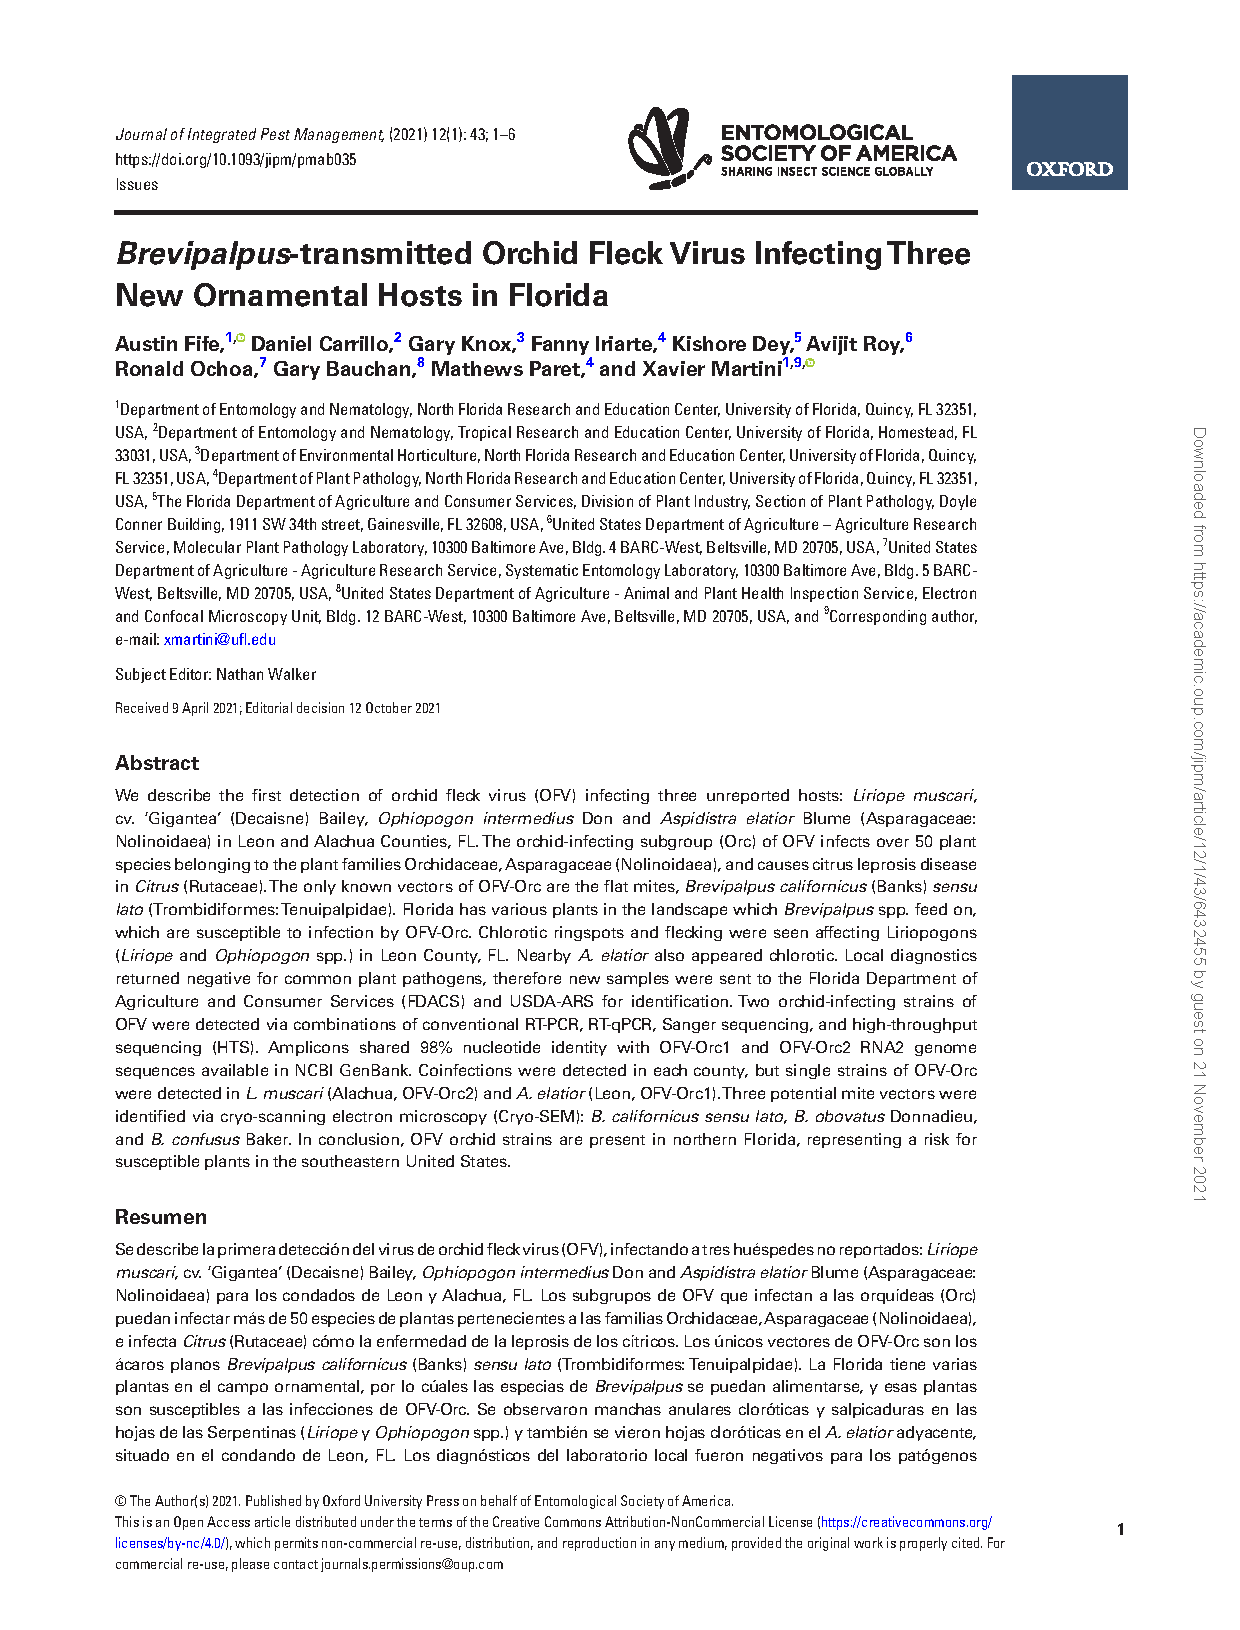
\includepdf[pages=1,pagecommand=\stepcounter{appendixVal}\stepcounter{appendixVal}\chapter {\textit{Brevipalpus}-TRANSMITTED ORCHID FLECK VIRUS INFECTING THREE NEW ORNAMENTAL HOSTS IN FLORIDA}, scale=0.93, offset=0.75 -1cm]{pubs/ofv_brevi_report.pdf}

\setlength{\footskip}{3.2em}

\includepdf[pages={2-last}, pagecommand={\thispagestyle{plain}}, fitpaper = true]{pubs/ofv_brevi_report.pdf}

\let\chapter\appendixChapter

\titleformat{\chapter }[hang]{\uppercase}{}{0pt}{\centering\realSingleSpace\ifdocBody CHAPTER \Alph{appendixVal}\\[-5pt] \fi}\raggedright\doublespacing

\docBodyfalse
\setcounter{secnumdepth}{-1}

\realSingleSpace

\hypertarget{references}{%
\chapter*{REFERENCES}\label{references}}
\addcontentsline{toc}{chapter}{REFERENCES}

\hypertarget{refs}{}
\begin{CSLReferences}{1}{1}
\leavevmode\vadjust pre{\hypertarget{ref-AbouAwad1985}{}}%
\textbf{Abou-Awad, B. A., and E. M. El-Banhawy}. \textbf{1985}. Susceptibility of the tomato russet mite, {\emph{Aculops lycopersici}} ({Acari}: {Eriophyidae}), in {Egypt} to methamidophos, pyridaphenthion, cypermethrin, dicofol and fenarimol. Experimental {\&} Applied Acarology. 1: 11--15, DOI:\href{https://doi.org/10.1007/bf01262195}{10.1007/bf01262195}.

\leavevmode\vadjust pre{\hypertarget{ref-Achor2001}{}}%
\textbf{Achor, D. S., R. Ochoa, E. F. Erbe, H. Aguilar, W. P. Wergin, and C. C. Childers}. \textbf{2001}. Relative advantages of low temperature versus ambient temperature scanning electron microscopy in the study of mite morphology. International Journal of Acarology. 27: 3--12, DOI:\href{https://doi.org/10.1080/01647950108684218}{10.1080/01647950108684218}.

\leavevmode\vadjust pre{\hypertarget{ref-Addesso2018}{}}%
\textbf{Addesso, K. M., A. L. Witcher, and D. C. Fare}. \textbf{2018}. Swirski mite controlled-release sachets as a pest management tool in container tree production. {HortTechnology}. 28: 391--398, DOI:\href{https://doi.org/10.21273/horttech03934-17}{10.21273/horttech03934-17}.

\leavevmode\vadjust pre{\hypertarget{ref-Adler1994}{}}%
\textbf{Adler, F. R., and R. Karban}. \textbf{1994}. Defended fortresses or moving targets? Another model of inducible defenses inspired by military metaphors. The American Naturalist. 144: 813--832, DOI:\href{https://doi.org/10.1086/285708}{10.1086/285708}.

\leavevmode\vadjust pre{\hypertarget{ref-Agrawal1997}{}}%
\textbf{Agrawal, A. A., and R. Karban}. \textbf{1997}. Domatia mediate plantarthropod mutualism. Nature. 387: 562--563, DOI:\href{https://doi.org/10.1038/42384}{10.1038/42384}.

\leavevmode\vadjust pre{\hypertarget{ref-Agrawal1999}{}}%
\textbf{Agrawal, A. A., and R. Karban}. \textbf{1999}. Advantages of induced plant defenses, pp. 45--62. \emph{In} Tollrain, R., Harvell, C.D. (eds.), The Ecology and Evolution of Inducible Defenses. Princeton University Press, Princeton, N.J.

\leavevmode\vadjust pre{\hypertarget{ref-Agrios2004}{}}%
\textbf{Agrios, G. N.} \textbf{2004}. \href{https://www.ebook.de/de/product/3267675/george_n_agrios_plant_pathology.html}{Plant pathology}. Academic Press.

\leavevmode\vadjust pre{\hypertarget{ref-Agut2018}{}}%
\textbf{Agut, B., V. Pastor, J. Jaques, and V. Flors}. \textbf{2018}. Can plant defence mechanisms provide new approaches for the sustainable control of the two-spotted spider mite {\emph{Tetranychus urticae}}? International Journal of Molecular Sciences. 19: 614, DOI:\href{https://doi.org/10.3390/ijms19020614}{10.3390/ijms19020614}.

\leavevmode\vadjust pre{\hypertarget{ref-Akyazi2017}{}}%
\textbf{Akyazi, R., E. A. Ueckermann, and O. E. Liburd}. \textbf{2017}. New report of {\emph{Brevipalpus yothersi}} ({Prostigmata}: {Tenuipalpidae}) on blueberry in {Florida}. Florida Entomologist. 100: 731--739, DOI:\href{https://doi.org/10.1653/024.100.0420}{10.1653/024.100.0420}.

\leavevmode\vadjust pre{\hypertarget{ref-Alavanja2004}{}}%
\textbf{Alavanja, M. C. R., J. A. Hoppin, and F. Kamel}. \textbf{2004}. Health effects of chronic pesticide exposure: Cancer and neurotoxicity. Annual Review of Public Health. 25: 155--197, DOI:\href{https://doi.org/10.1146/annurev.publhealth.25.101802.123020}{10.1146/annurev.publhealth.25.101802.123020}.

\leavevmode\vadjust pre{\hypertarget{ref-Alba2014}{}}%
\textbf{Alba, J. M., B. C. J. Schimmel, J. J. Glas, L. M. S. Ataide, M. L. Pappas, C. A. Villarroel, R. C. Schuurink, M. W. Sabelis, and M. R. Kant}. \textbf{2014}. Spider mites suppress tomato defenses downstream of jasmonate and salicylate independently of hormonal crosstalk. New Phytologist. 205: 828--840, DOI:\href{https://doi.org/10.1111/nph.13075}{10.1111/nph.13075}.

\leavevmode\vadjust pre{\hypertarget{ref-Alcivar2020}{}}%
\textbf{Alcı́var, J., N. C. Mesa, and C. Vásquez}. \textbf{2020}. First report of {\emph{Raoiella indica}} {Hirst} ({Acari}: {Tenuipalpidae}) in {Province} of {Manab{í}}, {Ecuador}. International Journal of Acarology. 46: 120--122, DOI:\href{https://doi.org/10.1080/01647954.2020.1719195}{10.1080/01647954.2020.1719195}.

\leavevmode\vadjust pre{\hypertarget{ref-Alipour2016}{}}%
\textbf{Alipour, Z., Y. Fathipour, and A. Farazmand}. \textbf{2016}. Age-stage predation capacity of {\emph{Phytoseiulus persimilis}} and {\emph{Amblyseius swirskii}} ({Acari}: {Phytoseiidae}) on susceptible and resistant rose cultivars. 42: 224--228, DOI:\href{https://doi.org/10.1080/01647954.2016.1171797}{10.1080/01647954.2016.1171797}.

\leavevmode\vadjust pre{\hypertarget{ref-Alipour2019}{}}%
\textbf{Alipour, Z., Y. Fathipour, A. Farazmand, and M. Khanamani}. \textbf{2019}. Resistant rose cultivar affects life table parameters of two-spotted spider mite and its predators {\emph{Phytoseiulus persimilis}} and {\emph{Amblyseius swirskii}} ({Phytoseiidae}). 24: 1620--1630, DOI:\href{https://doi.org/10.11158/saa.24.9.4}{10.11158/saa.24.9.4}.

\leavevmode\vadjust pre{\hypertarget{ref-Allington1968}{}}%
\textbf{Allington, W. B., R. Staples, and G. Viehmeyer}. \textbf{1968}. Transmission of {Rose rosette virus} by the eriophyid mite {\emph{Phyllocoptes fructiphilus}}. Journal of Economic Entomology. 61: 1137--1140, DOI:\href{https://doi.org/10.1093/jee/61.5.1137}{10.1093/jee/61.5.1137}.

\leavevmode\vadjust pre{\hypertarget{ref-Alves2005}{}}%
\textbf{Alves, E. B., N. F. B. Casarin, and C. Omoto}. \textbf{2005}. Mecanismos de dispers{ã}o de {\emph{Brevipalpus phoenicis}} ({Geijskes}) ({Acari}: {Tenuipalpidae}) em pomares de citros. Neotropical Entomology. 34: 89--96, DOI:\href{https://doi.org/10.1590/s1519-566x2005000100013}{10.1590/s1519-566x2005000100013}.

\leavevmode\vadjust pre{\hypertarget{ref-Alves2000}{}}%
\textbf{Alves, E. B., C. Omoto, and C. R. Franco}. \textbf{2000}. Resist{ê}ncia cruzada entre o dicofol e outros acaricidas em {\emph{Brevipalpus phoenicis}} ({Geijskes}) ({Acari}: {Tenuipalpidae}). Anais da Sociedade Entomol{ó}gica do Brasil. 29: 765--771, DOI:\href{https://doi.org/10.1590/s0301-80592000000400017}{10.1590/s0301-80592000000400017}.

\leavevmode\vadjust pre{\hypertarget{ref-Amarasinghe2019}{}}%
\textbf{Amarasinghe, G. K., M. A. Ayllón, Y. Bào, C. F. Basler, S. Bavari, K. R. Blasdell, T. Briese, P. A. Brown, A. Bukreyev, A. Balkema-Buschmann, U. J. Buchholz, C. Chabi-Jesus, K. Chandran, C. Chiapponi, I. Crozier, R. L. de Swart, R. G. Dietzgen, O. Dolnik, J. F. Drexler, R. Dürrwald, W. G. Dundon, W. P. Duprex, J. M. Dye, A. J. Easton, A. R. Fooks, P. B. H. Formenty, R. A. M. Fouchier, J. Freitas-Astúa, A. Griffiths, R. Hewson, M. Horie, T. H. Hyndman, D. Jiāng, E. W. Kitajima, G. P. Kobinger, H. Kondō, G. Kurath, I. V. Kuzmin, R. A. Lamb, A. Lavazza, B. Lee, D. Lelli, E. M. Leroy, J. Lǐ, P. Maes, S.-Y. L. Marzano, A. Moreno, E. Mühlberger, S. V. Netesov, N. Nowotny, A. Nylund, A. L. Økland, G. Palacios, B. Pályi, J. T. Pawęska, S. L. Payne, A. Prosperi, P. L. Ramos-González, B. K. Rima, P. Rota, D. Rubbenstroth, M. Shı̄, P. Simmonds, S. J. Smither, E. Sozzi, K. Spann, M. D. Stenglein, D. M. Stone, A. Takada, R. B. Tesh, K. Tomonaga, N. Tordo, J. S. Towner, B. van den Hoogen, N. Vasilakis, V. Wahl, P. J. Walker, L.-F. Wang, A. E. Whitfield, J. V. Williams, F. M. Zerbini, T. Zhāng, Y.-Z. Zhang, and J. H. Kuhn}. \textbf{2019}. Taxonomy of the order {Mononegavirales}: Update 2019. Archives of Virology. 164: 1967--1980, DOI:\href{https://doi.org/10.1007/s00705-019-04247-4}{10.1007/s00705-019-04247-4}.

\leavevmode\vadjust pre{\hypertarget{ref-Amaro2021}{}}%
\textbf{Amaro, G., E. G. Fidelis, R. S. da Silva, and C. M. de Medeiros}. \textbf{2021}. Current and potential geographic distribution of red palm mite ({\emph{Raoiella indica}} {Hirst}) in {Brazil}. Ecological Informatics. 65: 101396, DOI:\href{https://doi.org/10.1016/j.ecoinf.2021.101396}{10.1016/j.ecoinf.2021.101396}.

\leavevmode\vadjust pre{\hypertarget{ref-Ambrosio2008}{}}%
\textbf{Ambrósio, S. R., Y. Oki, V. C. G. Heleno, J. S. Chaves, P. G. B. D. Nascimento, J. E. Lichston, M. G. Constantino, E. M. Varanda, and F. B. D. Costa}. \textbf{2008}. Constituents of glandular trichomes of {\emph{Tithonia diversifolia}}: Relationships to herbivory and antifeedant activity. Phytochemistry. 69: 2052--2060, DOI:\href{https://doi.org/10.1016/j.phytochem.2008.03.019}{10.1016/j.phytochem.2008.03.019}.

\leavevmode\vadjust pre{\hypertarget{ref-Amrine1994}{}}%
\textbf{Amrine, J. W., and T. A. Stasny}. \textbf{1994}. Catalog of the {Eriophyoidea} ({Acarina}: {Prostigmata}) of the world. Indira Publishing House.

\leavevmode\vadjust pre{\hypertarget{ref-Amrine1996}{}}%
\textbf{Amrine Jr, J. W.} \textbf{1996}. \href{https://doi.org/10.1016/s1572-4379(96)80050-9}{{\emph{Phyllocoptes fructiphilus}} and biological control of multiflora rose}, pp. 741--749. \emph{In} Helle, W., Lundquist, E.E., Sabelis, M.W., Bruin, J. (eds.), Eriophyoid Mites. Their Biology, Natural Enemies, and Control, World Crop Pests. Elsevier.

\leavevmode\vadjust pre{\hypertarget{ref-Amrine2002}{}}%
\textbf{Amrine Jr, J. W.} \textbf{2002}. {\emph{Rosa multiflora}}. Biological control of invasive plants in the Eastern {United States}. 265--292.

\leavevmode\vadjust pre{\hypertarget{ref-Andrade2010}{}}%
\textbf{Andrade, D. J. de, C. A. L. de Oliveira, F. C. Pattaro, and D. S. Siqueira}. \textbf{2010}. Acaricidas utilizados na citricultura convencional e org{â}nica: Manejo da leprose e popula{ç}{õ}es de {á}caros fitose{í}deos. Revista Brasileira de Fruticultura. 32: 1028--1037, DOI:\href{https://doi.org/10.1590/s0100-29452011005000013}{10.1590/s0100-29452011005000013}.

\leavevmode\vadjust pre{\hypertarget{ref-Andrade2019}{}}%
\textbf{Andrade, D. J. de, E. B. Ribeiro, M. R. de Morais, and O. Z. Zanardi}. \textbf{2019}. Bioactivity of an oxymatrine-based commercial formulation against {\emph{Brevipalpus yothersi}} {Baker} and its effects on predatory mites in citrus groves. Ecotoxicology and Environmental Safety. 176: 339--345, DOI:\href{https://doi.org/10.1016/j.ecoenv.2019.03.118}{10.1016/j.ecoenv.2019.03.118}.

\leavevmode\vadjust pre{\hypertarget{ref-Anfoka2000}{}}%
\textbf{Anfoka, G. H.} \textbf{2000}. Benzo-(1,2,3)-thiadiazole-7-carbothioic acid {S}-methyl ester induces systemic resistance in tomato ({\emph{Lycopersicon esculentum}}. {Mill} cv. {Vollendung}) to {\emph{Cucumber mosaic virus}}. Crop Protection. 19: 401--405, DOI:\href{https://doi.org/10.1016/s0261-2194(00)00031-4}{10.1016/s0261-2194(00)00031-4}.

\leavevmode\vadjust pre{\hypertarget{ref-AnguelovaMerhar2008}{}}%
\textbf{Anguelova-Merhar, V. S., A. J. Westhuizen, and Z. A. Pretorius}. \textbf{2008}.\textbeta-1,3-glucanase and chitinase activities and the resistance response of wheat to leaf rust. Journal of Phytopathology. 149: 381--384, DOI:\href{https://doi.org/10.1111/j.1439-0434.2001.tb03866.x}{10.1111/j.1439-0434.2001.tb03866.x}.

\leavevmode\vadjust pre{\hypertarget{ref-Arena2016}{}}%
\textbf{Arena, G. D., P. L. Ramos-González, M. A. Nunes, M. Ribeiro-Alves, L. E. A. Camargo, E. W. Kitajima, M. A. Machado, and J. Freitas-Astúa}. \textbf{2016}. {Citrus leprosis virus} {C} infection results in hypersensitive-like response, suppression of the {JA}/{ET} plant defense pathway and promotion of the colonization of its mite vector. Frontiers in Plant Science. 7, DOI:\href{https://doi.org/10.3389/fpls.2016.01757}{10.3389/fpls.2016.01757}.

\leavevmode\vadjust pre{\hypertarget{ref-Arena2018}{}}%
\textbf{Arena, G. D., P. L. Ramos-González, L. A. Rogerio, M. Ribeiro-Alves, C. L. Casteel, J. Freitas-Astúa, and M. A. Machado}. \textbf{2018}. Making a better home: Modulation of plant defensive response by {\emph{Brevipalpus}} mites. Frontiers in Plant Science. 9, DOI:\href{https://doi.org/10.3389/fpls.2018.01147}{10.3389/fpls.2018.01147}.

\leavevmode\vadjust pre{\hypertarget{ref-Argolo2020}{}}%
\textbf{Argolo, P. S., A. M. Revynthi, M. A. Canon, M. M. Berto, D. J. Andrade, İ. Döker, A. Roda, and D. Carrillo}. \textbf{2020}. Potential of predatory mites for biological control of {\emph{Brevipalpus yothersi}} ({Acari}: {Tenuipalpidae}). Biological Control. 149: 104330, DOI:\href{https://doi.org/10.1016/j.biocontrol.2020.104330}{10.1016/j.biocontrol.2020.104330}.

\leavevmode\vadjust pre{\hypertarget{ref-Arimura2011}{}}%
\textbf{Arimura, G.-I., R. Ozawa, and M. E. Maffei}. \textbf{2011}. Recent advances in plant early signaling in response to herbivory. International Journal of Molecular Sciences. 12: 3723--3739, DOI:\href{https://doi.org/10.3390/ijms12063723}{10.3390/ijms12063723}.

\leavevmode\vadjust pre{\hypertarget{ref-Armstrong2005}{}}%
\textbf{Armstrong, K. F., and S. L. Ball}. \textbf{2005}. {DNA} barcodes for biosecurity: Invasive species identification. Philosophical Transactions of the Royal Society B: Biological Sciences. 360: 1813--1823, DOI:\href{https://doi.org/10.1098/rstb.2005.1713}{10.1098/rstb.2005.1713}.

\leavevmode\vadjust pre{\hypertarget{ref-Arthur2011}{}}%
\textbf{Arthur, A. L., A. D. Miller, and A. R. Weeks}. \textbf{2011}. Genetic markers indicate a new species complex of emerging pest mites in {Australian} grains. Annals of the Entomological Society of America. 104: 402--415, DOI:\href{https://doi.org/10.1603/an10065}{10.1603/an10065}.

\leavevmode\vadjust pre{\hypertarget{ref-Arthurs2009}{}}%
\textbf{Arthurs, S., C. L. McKenzie, J. Chen, M. Dogramaci, M. Brennan, K. Houben, and L. Osborne}. \textbf{2009}. Evaluation of {\emph{Neoseiulus cucumeris}} and {\emph{Amblyseius swirskii}} ({Acari}: {Phytoseiidae}) as biological control agents of chilli thrips, {\emph{Scirtothrips dorsalis}} ({Thysanoptera}: {Thripidae}) on pepper. 49: 91--96, DOI:\href{https://doi.org/10.1016/j.biocontrol.2009.01.002}{10.1016/j.biocontrol.2009.01.002}.

\leavevmode\vadjust pre{\hypertarget{ref-Ataide2016}{}}%
\textbf{Ataide, L. M. S., M. L. Pappas, B. C. J. Schimmel, A. Lopez-Orenes, J. M. Alba, M. V. A. Duarte, A. Pallini, R. C. Schuurink, and M. R. Kant}. \textbf{2016}. Induced plant-defenses suppress herbivore reproduction but also constrain predation of their offspring. Plant Science. 252: 300--310, DOI:\href{https://doi.org/10.1016/j.plantsci.2016.08.004}{10.1016/j.plantsci.2016.08.004}.

\leavevmode\vadjust pre{\hypertarget{ref-Avellaneda2019}{}}%
\textbf{Avellaneda, J., M. Dı́az, E. Coy-Barrera, D. Rodrı́guez, and C. Osorio}. \textbf{2019}. Rose volatile compounds allow the design of new control strategies for the {Western flower thrips} ({\emph{Frankliniella occidentalis}}). Journal of Pest Science., DOI:\href{https://doi.org/10.1007/s10340-019-01131-7}{10.1007/s10340-019-01131-7}.

\leavevmode\vadjust pre{\hypertarget{ref-Azevedo2016}{}}%
\textbf{Azevedo, L. H. de, R. D. C. Castilho, and G. J. de Moraes}. \textbf{2016}. Suitability of the litchi erineum mite, {\emph{Aceria litchii}} ({Keifer}), as prey for the mite {\emph{Phytoseius intermedius}} {Evans} \& {MacFarlane} ({Acari}: {Eriophyidae}, {Phytoseiidae}). 21: 270, DOI:\href{https://doi.org/10.11158/saa.21.3.2}{10.11158/saa.21.3.2}.

\leavevmode\vadjust pre{\hypertarget{ref-Babu2014}{}}%
\textbf{Babu, B., H. Dankers, E. Newberry, C. Baker, T. Schubert, G. Knox, and M. Paret}. \textbf{2014}. First report of {Rose rosette virus} associated with {Rose rosette disease} infecting knockout roses in {Florida}. Plant Disease. 98: 1449--1449, DOI:\url{https://doi.org/10.1094/PDIS-05-14-0501-PDN}.

\leavevmode\vadjust pre{\hypertarget{ref-Babu2016}{}}%
\textbf{Babu, B., A. Jeyaprakash, D. Jones, T. S. Schubert, C. Baker, B. K. Washburn, S. H. Miller, K. Poduch, G. W. Knox, F. M. Ochoa-Corona, and M. L. Paret}. \textbf{2016}. Development of a rapid, sensitive {TaqMan} real-time {RT}-{PCR} assay for the detection of {Rose rosette virus} using multiple gene targets. Journal of Virological Methods. 235: 41--50, DOI:\href{https://doi.org/10.1016/j.jviromet.2016.05.010}{10.1016/j.jviromet.2016.05.010}.

\leavevmode\vadjust pre{\hypertarget{ref-Babu2018}{}}%
\textbf{Babu, B., F. M. Ochoa-Corona, and M. L. Paret}. \textbf{2018}. Recombinase polymerase amplification applied to plant virus detection and potential implications. Analytical Biochemistry. 546: 72--77, DOI:\href{https://doi.org/10.1016/j.ab.2018.01.021}{10.1016/j.ab.2018.01.021}.

\leavevmode\vadjust pre{\hypertarget{ref-Babu2021}{}}%
\textbf{Babu, B., M. L. Paret, X. Martini, G. Knox, B. Riddle, L. Ritchie, J. Aldrich, M. Kalischuk, and S. da Silva}. \textbf{2021}. Impact of foliar application of acibenzolar s-methyl on rose rosette disease and rose plant quality., DOI:\href{https://doi.org/10.1094/pdis-01-21-0131-re}{10.1094/pdis-01-21-0131-re}.

\leavevmode\vadjust pre{\hypertarget{ref-Babu2017a}{}}%
\textbf{Babu, B., B. K. Washburn, T. S. Ertek, S. H. Miller, C. B. Riddle, G. W. Knox, F. M. Ochoa-Corona, J. Olson, Y. Z. Katırcıoğlu, and M. L. Paret}. \textbf{2017a}. A field based detection method for {Rose rosette virus} using isothermal probe-based reverse transcription-recombinase polymerase amplification assay. Journal of Virological Methods. 247: 81--90, DOI:\href{https://doi.org/10.1016/j.jviromet.2017.05.019}{10.1016/j.jviromet.2017.05.019}.

\leavevmode\vadjust pre{\hypertarget{ref-Babu2017b}{}}%
\textbf{Babu, B., B. K. Washburn, S. H. Miller, K. Poduch, T. Sarigul, G. W. Knox, F. M. Ochoa-Corona, and M. L. Paret}. \textbf{2017b}. A rapid assay for detection of {Rose rosette virus} using reverse transcription-recombinase polymerase amplification using multiple gene targets. Journal of Virological Methods. 240: 78--84, DOI:\href{https://doi.org/10.1016/j.jviromet.2016.11.014}{10.1016/j.jviromet.2016.11.014}.

\leavevmode\vadjust pre{\hypertarget{ref-Backus1988}{}}%
\textbf{Backus, E. A., W. B. Hunter, and C. N. Arne}. \textbf{1988}. Technique for staining leafhopper ({Homoptera}: {Cicadellidae}) salivary sheaths and eggs within unsectioned plant tissue. Journal of Economic Entomology. 81: 1819--1823, DOI:\href{https://doi.org/10.1093/jee/81.6.1819}{10.1093/jee/81.6.1819}.

\leavevmode\vadjust pre{\hypertarget{ref-Baker1949}{}}%
\textbf{Baker, E. W.} \textbf{1949}. The genus {\emph{Brevipalpus}} ({Acarina}: {Pseudoleptidae}). American Midland Naturalist. 42: 350, DOI:\href{https://doi.org/10.2307/2422013}{10.2307/2422013}.

\leavevmode\vadjust pre{\hypertarget{ref-Baker1987}{}}%
\textbf{Baker, E. W., and D. M. Tuttle}. \textbf{1987}. The false spider mites of {Mexico} ({Tenuipalpidae}: {Acari}). (technical report No. 1706). The {United States} Department of Agriculture - Agricultural Research Service.

\leavevmode\vadjust pre{\hypertarget{ref-Baker1979}{}}%
\textbf{Baker, R. T.} \textbf{1979}. Insecticide resistance in the peach silver mite {\emph{Aculus cornutus}} {(Banks)} ({Acari}: {Eriophyidae}). New Zealand Journal of Experimental Agriculture. 7: 405--406, DOI:\href{https://doi.org/10.1080/03015521.1979.10427117}{10.1080/03015521.1979.10427117}.

\leavevmode\vadjust pre{\hypertarget{ref-Baldwin1997}{}}%
\textbf{Baldwin, I. T., Z.-P. Zhang, N. Diab, T. E. Ohnmeiss, E. S. McCloud, G. Y. Lynds, and E. A. Schmelz}. \textbf{1997}. Quantification, correlations and manipulations of wound-induced changes in jasmonic acid and nicotine in {\emph{Nicotiana sylvestris}}. Planta. 201: 397--404, DOI:\href{https://doi.org/10.1007/s004250050082}{10.1007/s004250050082}.

\leavevmode\vadjust pre{\hypertarget{ref-Bastianel2010}{}}%
\textbf{Bastianel, M., V. M. Novelli, E. W. Kitajima, K. S. Kubo, R. B. Bassanezi, M. A. Machado, and J. Freitas-Astúa}. \textbf{2010}. {Citrus leprosis}: Centennial of an unusual mite{\textendash}virus pathosystem. Plant Disease. 94: 284--292, DOI:\href{https://doi.org/10.1094/pdis-94-3-0284}{10.1094/pdis-94-3-0284}.

\leavevmode\vadjust pre{\hypertarget{ref-Bates2015}{}}%
\textbf{Bates, D., M. Mächler, B. Bolker, and S. Walker}. \textbf{2015}. Fitting linear mixed-effects models using {lme4}. Journal of Statistical Software. 67: 1--48, DOI:\href{https://doi.org/10.18637/jss.v067.i01}{10.18637/jss.v067.i01}.

\leavevmode\vadjust pre{\hypertarget{ref-Bauchan2019}{}}%
\textbf{Bauchan, G. B., G. Otero-Colina, J. Hammond, R. Jordan, and R. Ochoa}. \textbf{2019}. {Rose rosette disease}: It all started with a small mite. Acta Horticulturae. 227--232, DOI:\href{https://doi.org/10.17660/actahortic.2019.1232.33}{10.17660/actahortic.2019.1232.33}.

\leavevmode\vadjust pre{\hypertarget{ref-Beard2012a}{}}%
\textbf{Beard, J. J., R. Ochoa, R. Bauchan G., D. Trice M., J. Redford A., W. Walters T., and C. Mitter}. \textbf{2012}. Flat mites of the world edition 2. (\url{http://idtools.org/id/mites/flatmites/}).

\leavevmode\vadjust pre{\hypertarget{ref-Beard2015}{}}%
\textbf{Beard, J. J., R. Ochoa, W. E. Braswell, and G. R. Bauchan}. \textbf{2015}. {\emph{Brevipalpus phoenicis}} {(Geijskes)} species complex ({Acari}: {Tenuipalpidae}) \textemdash a closer look. Zootaxa. 3944: 1, DOI:\href{https://doi.org/10.11646/zootaxa.3944.1.1}{10.11646/zootaxa.3944.1.1}.

\leavevmode\vadjust pre{\hypertarget{ref-Begtrup1972}{}}%
\textbf{Begtrup, J.} \textbf{1972}. Structure of a bacilliform virus in {\emph{Dendrobium}} as revealed by negative staining. Journal of Phytopathology. 75: 268--273, DOI:\href{https://doi.org/10.1111/j.1439-0434.1972.tb02623.x}{10.1111/j.1439-0434.1972.tb02623.x}.

\leavevmode\vadjust pre{\hypertarget{ref-Belliure2010}{}}%
\textbf{Belliure, B., M. W. Sabelis, and A. Janssen}. \textbf{2010}. Vector and virus induce plant responses that benefit a non-vector herbivore. Basic and Applied Ecology. 11: 162--169, DOI:\href{https://doi.org/10.1016/j.baae.2009.09.004}{10.1016/j.baae.2009.09.004}.

\leavevmode\vadjust pre{\hypertarget{ref-Bello2015}{}}%
\textbf{Bello, P. L. D., T. Ho, and I. E. Tzanetakis}. \textbf{2015}. The evolution of emaraviruses is becoming more complex: Seven segments identified in the causal agent of {Rose rosette disease}. Virus Research. 210: 241--244, DOI:\href{https://doi.org/10.1016/j.virusres.2015.08.009}{10.1016/j.virusres.2015.08.009}.

\leavevmode\vadjust pre{\hypertarget{ref-Beltran-Beltran2020}{}}%
\textbf{Beltran-Beltran, A. K., M. T. Santillán-Galicia, A. W. Guzmán-Franco, D. Teliz-Ortiz, M. A. Gutiérrez-Espinoza, F. Romero-Rosales, and P. L. Robles-Garcı́a}. \textbf{2020}. Incidence of {Citrus leprosis virus} {C} and {\emph{Orchid fleck dichorhavirus}} citrus strain in mites of the genus {\emph{Brevipalpus}} in {Mexico}. Journal of Economic Entomology. 113: 1576--1581, DOI:\href{https://doi.org/10.1093/jee/toaa007}{10.1093/jee/toaa007}.

\leavevmode\vadjust pre{\hypertarget{ref-Bensoussan2016}{}}%
\textbf{Bensoussan, N., M. E. Santamaria, V. Zhurov, I. Diaz, M. Grbić, and V. Grbić}. \textbf{2016}. Plant-herbivore interaction: Dissection of the cellular pattern of {\emph{Tetranychus urticae}} feeding on the host plant. Frontiers in Plant Science. 7, DOI:\href{https://doi.org/10.3389/fpls.2016.01105}{10.3389/fpls.2016.01105}.

\leavevmode\vadjust pre{\hypertarget{ref-Berenbaum1999}{}}%
\textbf{Berenbaum, M. R., and A. R. Zangerl}. \textbf{1999}. The ecology and evolution of inducible defenses, pp. 10--32. \emph{In} Tollrain, R., Harvell, C.D. (eds.),. Princeton University Press, Princeton, N.J.

\leavevmode\vadjust pre{\hypertarget{ref-Bergh2001}{}}%
\textbf{Bergh, J. C.} \textbf{2001}. Ecology and aerobiology of dispersing citrus rust mites ({Acari}: {Eriophyidae}) in central {Florida}. Environmental Entomology. 30: 318--326, DOI:\href{https://doi.org/10.1603/0046-225x-30.2.318}{10.1603/0046-225x-30.2.318}.

\leavevmode\vadjust pre{\hypertarget{ref-Bergh1997}{}}%
\textbf{Bergh, J. C., and C. W. Mccoy}. \textbf{1997}. Aerial dispersal of citrus rust mite ({Acari}: {Eriophyidae}) from {Florida} citrus groves. Environmental Entomology. 26: 256--264, DOI:\href{https://doi.org/10.1093/ee/26.2.256}{10.1093/ee/26.2.256}.

\leavevmode\vadjust pre{\hypertarget{ref-Bergougnoux2007}{}}%
\textbf{Bergougnoux, V., J.-C. Caissard, F. Jullien, J.-L. Magnard, G. Scalliet, J. M. Cock, P. Hugueney, and S. Baudino}. \textbf{2007}. Both the adaxial and abaxial epidermal layers of the rose petal emit volatile scent compounds. Planta. 226: 853--866, DOI:\href{https://doi.org/10.1007/s00425-007-0531-1}{10.1007/s00425-007-0531-1}.

\leavevmode\vadjust pre{\hypertarget{ref-Bhardwaj2021}{}}%
\textbf{Bhardwaj, G., I. Ravi, S. Kumar, and V. Sharma}. \textbf{2021}. Induction of \textbeta-1,3-glucanase and chitinase activity, cloning and their characterization in the defense response of {\emph{Cuminum cyminum}} plant against the fungal pathogen {\emph{Fusarium oxysporum}}. Archives of Phytopathology and Plant Protection. 1--16, DOI:\href{https://doi.org/10.1080/03235408.2021.1932016}{10.1080/03235408.2021.1932016}.

\leavevmode\vadjust pre{\hypertarget{ref-Bickford2007}{}}%
\textbf{Bickford, D., D. J. Lohman, N. S. Sodhi, P. K. L. Ng, R. Meier, K. Winker, K. K. Ingram, and I. Das}. \textbf{2007}. Cryptic species as a window on diversity and conservation. Trends in Ecology {\&} Evolution. 22: 148--155, DOI:\href{https://doi.org/10.1016/j.tree.2006.11.004}{10.1016/j.tree.2006.11.004}.

\leavevmode\vadjust pre{\hypertarget{ref-Biemond2013}{}}%
\textbf{Biemond, P. C., O. Oguntade, P. L. Kumar, T. J. Stomph, A. J. Termorshuizen, and P. C. Struik}. \textbf{2013}. Does the informal seed system threaten cowpea seed health? Crop Protection. 43: 166--174, DOI:\href{https://doi.org/10.1016/j.cropro.2012.09.007}{10.1016/j.cropro.2012.09.007}.

\leavevmode\vadjust pre{\hypertarget{ref-Biere2013}{}}%
\textbf{Biere, A., and A. E. Bennett}. \textbf{2013}. Three-way interactions between plants, microbes and insects. Functional Ecology. 27: 567--573, DOI:\href{https://doi.org/10.1111/1365-2435.12100}{10.1111/1365-2435.12100}.

\leavevmode\vadjust pre{\hypertarget{ref-Bischl2016}{}}%
\textbf{Bischl, B., M. Lang, L. Kotthoff, J. Schiffner, J. Richter, E. Studerus, G. Casalicchio, and Z. M. Jones}. \textbf{2016}. \href{https://jmlr.org/papers/v17/15-066.html}{{mlr}: Machine learning in {R}}. Journal of Machine Learning Research. 17: 1--5.

\leavevmode\vadjust pre{\hypertarget{ref-Blaazer2018}{}}%
\textbf{Blaazer, C. J. H., E. A. Villacis-Perez, R. Chafi, T. V. Leeuwen, M. R. Kant, and B. C. J. Schimmel}. \textbf{2018}. Why do herbivorous mites suppress plant defenses? Frontiers in Plant Science. 9, DOI:\href{https://doi.org/10.3389/fpls.2018.01057}{10.3389/fpls.2018.01057}.

\leavevmode\vadjust pre{\hypertarget{ref-Blanchfield2001}{}}%
\textbf{Blanchfield, A. L., A. M. Mackenzie, A. Gibbs, H. Kondo, T. Tamada, and C. R. Wilson}. \textbf{2001}. Identification of {Orchid fleck virus} by reverse transcriptase-polymerase chain reaction and analysis of isolate relationships. Journal of Phytopathology. 149: 713--718, DOI:\href{https://doi.org/10.1046/j.1439-0434.2001.00702.x}{10.1046/j.1439-0434.2001.00702.x}.

\leavevmode\vadjust pre{\hypertarget{ref-Boer2004a}{}}%
\textbf{Boer, J. G. de, and M. Dicke}. \textbf{2004a}. The role of methyl salicylate in prey searching behavior of the predatory mite {\emph{Phytoseiulus persimilis}}. Journal of Chemical Ecology. 30: 255--271, DOI:\href{https://doi.org/10.1023/b:joec.0000017976.60630.8c}{10.1023/b:joec.0000017976.60630.8c}.

\leavevmode\vadjust pre{\hypertarget{ref-Boer2004b}{}}%
\textbf{Boer, J. G. de, and M. Dicke}. \textbf{2004b}. Experience with methyl salicylate affects behavioural responses of a predatory mite to blends of herbivore-induced plant volatiles. Entomologia Experimentalis et Applicata. 110: 181--189, DOI:\href{https://doi.org/10.1111/j.0013-8703.2004.00133.x}{10.1111/j.0013-8703.2004.00133.x}.

\leavevmode\vadjust pre{\hypertarget{ref-Boer2005}{}}%
\textbf{Boer, J. G. de, and M. Dicke}. \textbf{2005}. Information use by the predatory mite {\emph{Phytoseiulus persimilis}} {({Acari}: {Phytoseiidae})}, a specialised natural enemy of herbivorous spider mites. Applied Entomology and Zoology. 40: 1--12, DOI:\href{https://doi.org/10.1303/aez.2005.1}{10.1303/aez.2005.1}.

\leavevmode\vadjust pre{\hypertarget{ref-Bolckmans2005}{}}%
\textbf{Bolckmans, K., Y. van Houten, and H. Hoogerbrugge}. \textbf{2005}. Biological control of whiteflies and western thrips in greenhouse sweet peppers with the phytoseiid predatory mite {\emph{Amblyseius swirskii}} {Athias-Henriot} ({Acari}: {Phytoseiidae}), pp. 555--565. \emph{In} Hoddle, M.S. (ed.), Second International Symposium on Biological Control of Arthropods. USDA Forest Service; USDA Forest Service Publication Forest Health Technology Enterprise Team.

\leavevmode\vadjust pre{\hypertarget{ref-Boller2009}{}}%
\textbf{Boller, T., and G. Felix}. \textbf{2009}. A renaissance of elicitors: Perception of microbe-associated molecular patterns and danger signals by pattern-recognition receptors. Annual Review of Plant Biology. 60: 379--406, DOI:\href{https://doi.org/10.1146/annurev.arplant.57.032905.105346}{10.1146/annurev.arplant.57.032905.105346}.

\leavevmode\vadjust pre{\hypertarget{ref-Bolton2018}{}}%
\textbf{Bolton, S. J., G. R. Bauchan, P. E. Chetverikov, R. Ochoa, and H. Klompen}. \textbf{2018}. A rudimentary sheath for the smallest of "biting" chelicerae: The mouthparts of {\emph{Cunliffea}} ({Nematalycidae}) and a new hypothesis on the origin of the stylet sheath of {Eriophyoidea} ({Acariformes}). International Journal of Acarology. 44: 374--381, DOI:\href{https://doi.org/10.1080/01647954.2018.1488274}{10.1080/01647954.2018.1488274}.

\leavevmode\vadjust pre{\hypertarget{ref-Boom2004}{}}%
\textbf{Boom, C. E. M. V. D., T. A. V. Beek, M. A. Posthumus, A. D. Groot, and M. Dicke}. \textbf{2004}. Qualitative and quantitative variation among volatile profiles induced by {\emph{Tetranychus urticae}} feeding on plants from various families. Journal of Chemical Ecology. 30: 69--89, DOI:\href{https://doi.org/10.1023/b:joec.0000013183.72915.99}{10.1023/b:joec.0000013183.72915.99}.

\leavevmode\vadjust pre{\hypertarget{ref-Boom2002}{}}%
\textbf{Boom, C. E. M. van den, T. A. van Beek, and M. Dicke}. \textbf{2002}. Attraction of {\emph{Phytoseiulus persimilis}} ({Acari}: {Phytoseiidae}) towards volatiles from various {\emph{Tetranychus urticae}}-infested plant species. Bulletin of Entomological Research. 92, DOI:\href{https://doi.org/10.1079/ber2002193}{10.1079/ber2002193}.

\leavevmode\vadjust pre{\hypertarget{ref-Bouagga2018}{}}%
\textbf{Bouagga, S., A. Urbaneja, and M. Pérez-Hedo}. \textbf{2018}. Combined use of predatory mirids with {\emph{Amblyseius swirskii}} ({Acari}: {Phytoseiidae}) to enhance pest management in sweet pepper. Journal of Economic Entomology. 111: 1112--1120, DOI:\href{https://doi.org/10.1093/jee/toy072}{10.1093/jee/toy072}.

\leavevmode\vadjust pre{\hypertarget{ref-Boubou2012}{}}%
\textbf{Boubou, A., A. Migeon, G. K. Roderick, P. Auger, J.-M. Cornuet, S. Magalhães, and M. Navajas}. \textbf{2012}. Test of colonisation scenarios reveals complex invasion history of the red tomato spider mite {\emph{Tetranychus evansi}}. {PLoS} {ONE}. 7: e35601, DOI:\href{https://doi.org/10.1371/journal.pone.0035601}{10.1371/journal.pone.0035601}.

\leavevmode\vadjust pre{\hypertarget{ref-Boubou2010}{}}%
\textbf{Boubou, A., A. Migeon, G. K. Roderick, and M. Navajas}. \textbf{2010}. Recent emergence and worldwide spread of the red tomato spider mite, {\emph{Tetranychus evansi}}: Genetic variation and multiple cryptic invasions. Biological Invasions. 13: 81--92, DOI:\href{https://doi.org/10.1007/s10530-010-9791-y}{10.1007/s10530-010-9791-y}.

\leavevmode\vadjust pre{\hypertarget{ref-Bratsch2015}{}}%
\textbf{Bratsch, S. A., B. E. Lockhart, and C. Ishimaru}. \textbf{2015}. Confirmation of first report of {Orchid fleck virus} in {\emph{Phalaenopsis}} hybrid orchids in the {USA}. Plant Health Progress. 16: 146--148, DOI:\href{https://doi.org/10.1094/php-br-15-0018}{10.1094/php-br-15-0018}.

\leavevmode\vadjust pre{\hypertarget{ref-Bronner1991}{}}%
\textbf{Bronner, R., E. Westphal, and F. Dreger}. \textbf{1991a}. Enhanced peroxidase activity associated with the hypersensitive response of {\emph{Solanum dulcamara}} to the gall mite {\emph{Aceria cladophthirus}} ({Acari}: {Eriophyoidea}). Canadian Journal of Botany. 69: 2192--2196, DOI:\href{https://doi.org/10.1139/b91-275}{10.1139/b91-275}.

\leavevmode\vadjust pre{\hypertarget{ref-Bronner1991a}{}}%
\textbf{Bronner, R., E. Westphal, and F. Dreger}. \textbf{1991b}. Pathogenesis-related proteins in {\emph{Solanum dulcamara}} {L.} Resistant to the gall mite {\emph{Aceria cladophthirus}} ({Nalepa})(syn {\emph{Eriophyes cladophthirus}} {Nal.}). Physiological and molecular plant pathology.

\leavevmode\vadjust pre{\hypertarget{ref-Broussard2007}{}}%
\textbf{Broussard, M. C.} \textbf{2007}. A horticultural study of {\emph{Liriope}} and {\emph{Ophiopogon}}: Nomenclature, morphology, and culture (PhD thesis). Louisiana State University, Department of Horticulture.

\leavevmode\vadjust pre{\hypertarget{ref-Buitenhuis2014}{}}%
\textbf{Buitenhuis, R., E. Glemser, and A. Brommit}. \textbf{2014}. Practical placement improves the performance of slow release sachets of {\emph{Neoseiulus cucumeris}}. Biocontrol Science and Technology. 24: 1153--1166, DOI:\href{https://doi.org/10.1080/09583157.2014.930726}{10.1080/09583157.2014.930726}.

\leavevmode\vadjust pre{\hypertarget{ref-Buitenhuis2015}{}}%
\textbf{Buitenhuis, R., G. Murphy, L. Shipp, and C. Scott-Dupree}. \textbf{2015}. {\emph{Amblyseius swirskii}} in greenhouse production systems: A floricultural perspective. Experimental and Applied Acarology. 65: 451--464, DOI:\href{https://doi.org/10.1007/s10493-014-9869-9}{10.1007/s10493-014-9869-9}.

\leavevmode\vadjust pre{\hypertarget{ref-Buitenhuis2010}{}}%
\textbf{Buitenhuis, R., L. Shipp, and C. Scott-Dupree}. \textbf{2010}. Dispersal of {\emph{Amblyseius swirskii}} {Athias}-{Henriot} ({Acari}: {Phytoseiidae}) on potted greenhouse chrysanthemum. Biological Control. 52: 110--114, DOI:\href{https://doi.org/10.1016/j.biocontrol.2009.10.007}{10.1016/j.biocontrol.2009.10.007}.

\leavevmode\vadjust pre{\hypertarget{ref-Buitenhuis2013}{}}%
\textbf{Buitenhuis, R., L. Shipp, C. Scott-Dupree, A. Brommit, and W. Lee}. \textbf{2013}. Host plant effects on the behaviour and performance of {\emph{Amblyseius swirskii}} ({Acari}: {Phytoseiidae}). Experimental and Applied Acarology. 62: 171--180, DOI:\href{https://doi.org/10.1007/s10493-013-9735-1}{10.1007/s10493-013-9735-1}.

\leavevmode\vadjust pre{\hypertarget{ref-vanBuuren2011}{}}%
\textbf{Buuren, S. van, and K. Groothuis-Oudshoorn}. \textbf{2011}. \href{https://www.jstatsoft.org/v45/i03/}{{mice}: {Multivariate} {Imputation} by {Chained} {Equations} in {R}}. Journal of Statistical Software. 45: 1--67.

\leavevmode\vadjust pre{\hypertarget{ref-Byrne2019}{}}%
\textbf{Byrne, D. H., P. E. Klein, C. Hall, M. Windham, F. M. Ochoa-Corona, J. Olson, M. Paret, B. Babu, G. Knox, R. Jordan, J. Hammond, K. Ong, R. Ochoa, G. B. Bauchan, T. Evans, A. Windham, F. Hale, M. A. Palma, L. Ribera, and H. B. Pemberton}. \textbf{2019}. Combating {Rose rosette disease} {US} national project. Acta Horticulturae. 203--212, DOI:\href{https://doi.org/10.17660/actahortic.2019.1232.30}{10.17660/actahortic.2019.1232.30}.

\leavevmode\vadjust pre{\hypertarget{ref-Byrne2018}{}}%
\textbf{Byrne, D. H., P. Klein, M. Yan, E. Young, J. Lau, K. Ong, M. Shires, J. Olson, M. Windham, T. Evans, and D. Novick}. \textbf{2018}. Challenges of breeding {Rose rosette}-resistant roses. {HortScience}. 53: 604--608, DOI:\href{https://doi.org/10.21273/hortsci12553-17}{10.21273/hortsci12553-17}.

\leavevmode\vadjust pre{\hypertarget{ref-Calvet2020}{}}%
\textbf{Calvet, É. C., D. B. Lima, J. W. S. Melo, and M. G. C. G. Jr.} \textbf{2020}. Host plant discrimination through mobility parameters by eriophyoid mites. Systematic and Applied Acarology. 25: 1541--1551, DOI:\href{https://doi.org/10.11158/saa.25.9.2}{10.11158/saa.25.9.2}.

\leavevmode\vadjust pre{\hypertarget{ref-Calvo2010}{}}%
\textbf{Calvo, F. J., K. Bolckmans, and J. E. Belda}. \textbf{2010}. Control of {\emph{Bemisia tabaci}} and {\emph{Frankliniella occidentalis}} in cucumber by {\emph{Amblyseius swirskii}}. {BioControl}. 56: 185--192, DOI:\href{https://doi.org/10.1007/s10526-010-9319-5}{10.1007/s10526-010-9319-5}.

\leavevmode\vadjust pre{\hypertarget{ref-Calvo2014}{}}%
\textbf{Calvo, F. J., M. Knapp, Y. M. van Houten, H. Hoogerbrugge, and J. E. Belda}. \textbf{2014}. {\emph{Amblyseius swirskii}}: What made this predatory mite such a successful biocontrol agent? Experimental and Applied Acarology. 65: 419--433, DOI:\href{https://doi.org/10.1007/s10493-014-9873-0}{10.1007/s10493-014-9873-0}.

\leavevmode\vadjust pre{\hypertarget{ref-Calvo2007}{}}%
\textbf{Calvo, J., and J. E. Belda}. \textbf{2007}. {\emph{Amblyseius swirskii}}, un depredador para el control de la mosca blanca y trips en cultivos hort{í}colas. Phytoma Espa{ñ}a: La revista profesional de sanidad vegetal. 58--63.

\leavevmode\vadjust pre{\hypertarget{ref-Campos2002}{}}%
\textbf{Campos, F. J., and C. Omoto}. \textbf{2002}. Resistance to hexythiazox in {\emph{Brevipalpus phoenicis}} ({Acari}: {Tenuipalpidae}) from {Brazilian} citrus. Experimental and Applied Acarology. 26: 243--251, DOI:\href{https://doi.org/10.1023/a:1021103209193}{10.1023/a:1021103209193}.

\leavevmode\vadjust pre{\hypertarget{ref-Card2018}{}}%
\textbf{Card, D. C., B. W. Perry, R. H. Adams, D. R. Schield, A. S. Young, A. L. Andrew, T. Jezkova, G. I. M. Pasquesi, N. R. Hales, M. R. Walsh, M. R. Rochford, F. J. Mazzotti, K. M. Hart, M. E. Hunter, and T. A. Castoe}. \textbf{2018}. Novel ecological and climatic conditions drive rapid adaptation in invasive {Florida} {Burmese} pythons. 27: 4744--4757, DOI:\href{https://doi.org/10.1111/mec.14885}{10.1111/mec.14885}.

\leavevmode\vadjust pre{\hypertarget{ref-Carrillo2011a}{}}%
\textbf{Carrillo, D., J. H. Frank, J. C. V. Rodrigues, and J. E. Peña}. \textbf{2011a}. A review of the natural enemies of the red palm mite, {\emph{Raoiella indica}} ({Acari}: {Tenuipalpidae}). Experimental and Applied Acarology. 57: 347--360, DOI:\href{https://doi.org/10.1007/s10493-011-9499-4}{10.1007/s10493-011-9499-4}.

\leavevmode\vadjust pre{\hypertarget{ref-Carrillo2011b}{}}%
\textbf{Carrillo, D., D. Navia, F. Ferragut, and J. E. Peña}. \textbf{2011b}. First report of {\emph{Raoiella indica}} ({Acari}: {Tenuipalpidae}) in {Colombia}. Florida Entomologist. 94: 370--371, DOI:\href{https://doi.org/10.1653/024.094.0241}{10.1653/024.094.0241}.

\leavevmode\vadjust pre{\hypertarget{ref-Carrillo2011}{}}%
\textbf{Carrillo, D., and J. E. Peña}. \textbf{2011}. Prey-stage preferences and functional and numerical responses of {\emph{Amblyseius largoensis}} ({Acari: Phytoseiidae}) to {\emph{Raoiella indica}} ({Acari}: {Tenuipalpidae}). Experimental and Applied Acarology. 57: 361--372, DOI:\href{https://doi.org/10.1007/s10493-011-9488-7}{10.1007/s10493-011-9488-7}.

\leavevmode\vadjust pre{\hypertarget{ref-Cedola2001}{}}%
\textbf{Cédola, C. V., N. E. Sánchez, and G. G. Liljesthröm}. \textbf{2001}. Effect of tomato leaf hairiness on functional and numerical response of {\emph{Neoseiulus californicus}} ({Acari}: {Phytoseiidae}). Experimental and Applied Acarology. 25: 819--831, DOI:\href{https://doi.org/10.1023/a:1020499624661}{10.1023/a:1020499624661}.

\leavevmode\vadjust pre{\hypertarget{ref-ChabiJesus2018}{}}%
\textbf{Chabi-Jesus, C., P. L. Ramos-González, A. D. Tassi, O. Guerra-Peraza, E. W. Kitajima, R. Harakava, J. E. A. Beserra, R. B. Salaroli, and J. Freitas-Astúa}. \textbf{2018}. Identification and characterization of {Citrus Chlorotic Spot Virus}, a new {\emph{Dichorhavirus}} associated with {Citrus leprosis}-like symptoms. Plant Disease. 102: 1588--1598, DOI:\href{https://doi.org/10.1094/pdis-09-17-1425-re}{10.1094/pdis-09-17-1425-re}.

\leavevmode\vadjust pre{\hypertarget{ref-Chagas2003}{}}%
\textbf{Chagas, C. M., E. W. Kitajima, and J. C. V. Rodrigues}. \textbf{2003}. {Coffee ringspot virus} vectored by {\emph{Brevipalpus phoenicis}} ({Acari}: {Tenuipalpidae}) in coffee. Experimental and Applied Acarology. 30: 203--213, DOI:\href{https://doi.org/10.1023/b:appa.0000006549.87310.41}{10.1023/b:appa.0000006549.87310.41}.

\leavevmode\vadjust pre{\hypertarget{ref-Chambers2019}{}}%
\textbf{Chambers, A. H., P. Moon, V. Edmond, and E. Bassil}. \textbf{2019}. Vanilla cultivation in southern {Florida}. {EDIS}. 2019: 7, DOI:\href{https://doi.org/10.32473/edis-hs1348-2019}{10.32473/edis-hs1348-2019}.

\leavevmode\vadjust pre{\hypertarget{ref-Chang1976}{}}%
\textbf{Chang, M. U., Arai. Kei, Doi. Yoji, and Yora. Kiyoshi}. \textbf{1976}. Morphology and intracellular appearance of {Orchid fleck virus}. Japanese Journal of Phytopathology. 42: 156--157, DOI:\href{https://doi.org/10.3186/jjphytopath.42.156}{10.3186/jjphytopath.42.156}.

\leavevmode\vadjust pre{\hypertarget{ref-Chang2019}{}}%
\textbf{Chang, W.} \textbf{2019}. \href{https://CRAN.R-project.org/package=webshot}{{webshot:} Take screenshots of web pages}.

\leavevmode\vadjust pre{\hypertarget{ref-Chapman2017}{}}%
\textbf{Chapman, D., B. V. Purse, H. E. Roy, and J. M. Bullock}. \textbf{2017}. Global trade networks determine the distribution of invasive non-native species. Global Ecology and Biogeography. 26: 907--917, DOI:\href{https://doi.org/10.1111/geb.12599}{10.1111/geb.12599}.

\leavevmode\vadjust pre{\hypertarget{ref-Chase2009}{}}%
\textbf{Chase, Mark. W., James. L. Reveal, and M. F. Fay}. \textbf{2009}. A subfamilial classification for the expanded asparagalean families {Amaryllidaceae}, {Asparagaceae} and {Xanthorrhoeaceae}. Botanical Journal of the Linnean Society. 161: 132--136, DOI:\href{https://doi.org/10.1111/j.1095-8339.2009.00999.x}{10.1111/j.1095-8339.2009.00999.x}.

\leavevmode\vadjust pre{\hypertarget{ref-Chen2006}{}}%
\textbf{Chen, T.-Y., J. V. French, T.-X. Liu, and J. V. da Graça}. \textbf{2006}. Predation of {\emph{Galendromus helveolus}} ({Acari}: {Phytoseiidae}) on {\emph{Brevipalpus californicus}} ({Acari}: {Tenuipalpidae}). Biocontrol Science and Technology. 16: 753--759, DOI:\href{https://doi.org/10.1080/09583150600700172}{10.1080/09583150600700172}.

\leavevmode\vadjust pre{\hypertarget{ref-Chetverikov2012}{}}%
\textbf{Chetverikov, P. E.} \textbf{2012}. Confocal laser scanning microscopy technique for the study of internal genitalia and external morphology of eriophyoid mites ({Acari}: {Eriophyoidea}). Zootaxa. 3453: 56--68.

\leavevmode\vadjust pre{\hypertarget{ref-Chetverikov2012a}{}}%
\textbf{Chetverikov, P. E., F. Beaulieu, T. Cvrković, B. Vidović, and R. Petanović}. \textbf{2012}. {\emph{Oziella sibirica}} ({Acari}: {Eriophyoidea}: {Phytoptidae}), a new eriophyoid mite species described using confocal microscopy, {COI} barcoding and {3D} surface reconstruction. Zootaxa. 3560: 41--60.

\leavevmode\vadjust pre{\hypertarget{ref-Chigira2005}{}}%
\textbf{Chigira, A., and K. Miura}. \textbf{2005}. Detection of {``{\emph{Candidatus}} {Cardinium}''} bacteria from the haploid host {\emph{Brevipalpus californicus}} ({Acari}: {Tenuipalpidae}) and effect on the host. Experimental and Applied Acarology. 37: 107--116, DOI:\href{https://doi.org/10.1007/s10493-005-0592-4}{10.1007/s10493-005-0592-4}.

\leavevmode\vadjust pre{\hypertarget{ref-Childers1994}{}}%
\textbf{Childers, C. C.} \textbf{1994}. Feeding injury to {'Robinson'} tangerine leaves by {\emph{Brevipalpus}} mites ({Acari}: {Tenuipalpidae}) in {Florida} and evaluation of chemical control on citrus. Florida Entomologist. 77: 265--271.

\leavevmode\vadjust pre{\hypertarget{ref-Childers2003c}{}}%
\textbf{Childers, C. C., and K. S. Derrick}. \textbf{2003}. {\emph{Brevipalpus}} mites as vectors of unassigned {Rhabdoviruses} in various crops. Experimental and Applied Acarology. 30: 1--3, DOI:\href{https://doi.org/10.1023/b:appa.0000006542.96404.63}{10.1023/b:appa.0000006542.96404.63}.

\leavevmode\vadjust pre{\hypertarget{ref-Childers2003b}{}}%
\textbf{Childers, C. C., J. V. French, and J. C. V. Rodrigues}. \textbf{2003a}. {\emph{Brevipalpus californicus}}, {\emph{B. obovatus}}, {\emph{B. phoenicis}}, and {\emph{B. lewisi}} ({Acari}: {Tenuipalpidae}): A review of their biology, feeding injury and economic importance. Experimental and Applied Acarology. 30: 5--28, DOI:\href{https://doi.org/10.1023/b:appa.0000006543.34042.b4}{10.1023/b:appa.0000006543.34042.b4}.

\leavevmode\vadjust pre{\hypertarget{ref-Childers2011}{}}%
\textbf{Childers, C. C., and J. C. V. Rodrigues}. \textbf{2011}. An overview of {\emph{Brevipalpus}} ({Acari}: {Tenuipalpidae}) and the plant viruses they transmit. Zoosymposia. 6: 180--192, DOI:\href{https://doi.org/10.11646/zoosymposia.6.1.28}{10.11646/zoosymposia.6.1.28}.

\leavevmode\vadjust pre{\hypertarget{ref-Childers2003}{}}%
\textbf{Childers, C. C., J. C. V. Rodrigues, K. S. Derrick, D. S. Achor, J. V. French, W. C. Welbourn, R. Ochoa, and E. W. Kitajima}. \textbf{2003b}. {Citrus leprosis} and its status in {Florida} and {Texas}: Past and present. Experimental and Applied Acarology. 30: 181--202, DOI:\href{https://doi.org/10.1023/b:appa.0000006548.01625.72}{10.1023/b:appa.0000006548.01625.72}.

\leavevmode\vadjust pre{\hypertarget{ref-Childers2003a}{}}%
\textbf{Childers, C. C., J. C. V. Rodrigues, and W. C. Welbourn}. \textbf{2003c}. Host plants of {\emph{Brevipalpus californicus}}, {\emph{B. obovatus}}, and {\emph{B. phoenicis}} ({Acari}: {Tenuipalpidae}) and their potential involvement in the spread of viral diseases vectored by these mites. Experimental and Applied Acarology. 30: 29--105, DOI:\href{https://doi.org/10.1023/b:appa.0000006544.10072.01}{10.1023/b:appa.0000006544.10072.01}.

\leavevmode\vadjust pre{\hypertarget{ref-Chisholm2006}{}}%
\textbf{Chisholm, S. T., G. Coaker, B. Day, and B. J. Staskawicz}. \textbf{2006}. Host-microbe interactions: Shaping the evolution of the plant immune response. Cell. 124: 803--814, DOI:\href{https://doi.org/10.1016/j.cell.2006.02.008}{10.1016/j.cell.2006.02.008}.

\leavevmode\vadjust pre{\hypertarget{ref-Choh2007}{}}%
\textbf{Choh, Y., and J. Takabayashi}. \textbf{2007}. Duration of priming of two indirect plant defenses. Plant Signaling {\&} Behavior. 2: 13--14, DOI:\href{https://doi.org/10.4161/psb.2.1.3605}{10.4161/psb.2.1.3605}.

\leavevmode\vadjust pre{\hypertarget{ref-Chow2010}{}}%
\textbf{Chow, A., A. Chau, and K. M. Heinz}. \textbf{2010}. Compatibility of {\emph{Amblyseius (Typhlodromips) swirskii}} ({Athias-Henriot}) ({Acari: Phytoseiidae}) and {\emph{Orius insidiosus}} ({Hemiptera}: {Anthocoridae}) for biological control of {\emph{Frankliniella occidentalis}} ({Thysanoptera:} {Thripidae}) on roses. Biological Control. 53: 188--196, DOI:\href{https://doi.org/10.1016/j.biocontrol.2009.12.008}{10.1016/j.biocontrol.2009.12.008}.

\leavevmode\vadjust pre{\hypertarget{ref-Cole1999}{}}%
\textbf{Cole, D. L.} \textbf{1999}. The efficacy of acibenzolar-{S}-methyl, an inducer of systemic acquired resistance, against bacterial and fungal diseases of tobacco. Crop Protection. 18: 267--273, DOI:\href{https://doi.org/10.1016/s0261-2194(99)00026-5}{10.1016/s0261-2194(99)00026-5}.

\leavevmode\vadjust pre{\hypertarget{ref-Conners1941}{}}%
\textbf{Conners, L.} \textbf{1941}. Twentieth annual report of the {Canadian} plant report survey 1940. Dominion Can. Dept. Agr. Sci. Serv.

\leavevmode\vadjust pre{\hypertarget{ref-Conrath2006}{}}%
\textbf{Conrath, U., G. J. M. Beckers, V. Flors, P. Garcı́a-Agustı́n, G. Jakab, F. Mauch, M.-A. Newman, C. M. J. Pieterse, B. Poinssot, M. J. Pozo, A. Pugin, U. Schaffrath, J. Ton, D. Wendehenne, L. Zimmerli, and B. Mauch-Mani}. \textbf{2006}. Priming: Getting ready for battle. Molecular Plant-Microbe Interactions{\textregistered}. 19: 1062--1071, DOI:\href{https://doi.org/10.1094/mpmi-19-1062}{10.1094/mpmi-19-1062}.

\leavevmode\vadjust pre{\hypertarget{ref-UGA2018}{}}%
\textbf{(\href{https://roserosette.org/control/}{Control - rose rosette}) University of Georgia - Center for Invasive Species and Ecosystem Health}. \textbf{2018}. \href{https://roserosette.org/control/}{Control - rose rosette}.

\leavevmode\vadjust pre{\hypertarget{ref-Cook2019}{}}%
\textbf{Cook, G., W. Kirkman, R. Clase, C. Steyn, E. Basson, P. H. Fourie, S. D. Moore, T. G. Grout, E. Carstens, and V. Hattingh}. \textbf{2019}. {Orchid fleck virus} associated with the first case of {Citrus leprosis}-{N} in {South Africa}. European Journal of Plant Pathology. 155: 1373--1379, DOI:\href{https://doi.org/10.1007/s10658-019-01854-4}{10.1007/s10658-019-01854-4}.

\leavevmode\vadjust pre{\hypertarget{ref-Cook2007}{}}%
\textbf{Cook, S. M., Z. R. Khan, and J. A. Pickett}. \textbf{2007}. The use of push-pull strategies in integrated pest management. 52: 375--400, DOI:\href{https://doi.org/10.1146/annurev.ento.52.110405.091407}{10.1146/annurev.ento.52.110405.091407}.

\leavevmode\vadjust pre{\hypertarget{ref-Coomes2015}{}}%
\textbf{Coomes, O. T., S. J. McGuire, E. Garine, S. Caillon, D. McKey, E. Demeulenaere, D. Jarvis, G. Aistara, A. Barnaud, P. Clouvel, L. Emperaire, S. Louafi, P. Martin, F. Massol, M. Pautasso, C. Violon, and J. Wencélius}. \textbf{2015}. Farmer seed networks make a limited contribution to agriculture? Four common misconceptions. Food Policy. 56: 41--50, DOI:\href{https://doi.org/10.1016/j.foodpol.2015.07.008}{10.1016/j.foodpol.2015.07.008}.

\leavevmode\vadjust pre{\hypertarget{ref-Correa2005}{}}%
\textbf{Correa, R. S. B., J. C. Moraes, A. M. Auad, and G. A. Carvalho}. \textbf{2005}. Silicon and acibenzolar-{S}-methyl as resistance inducers in cucumber, against the whitefly {\emph{Bemisia tabaci}} ({Gennadius}) ({Hemiptera}: {Aleyrodidae}) biotype {B}. Neotropical Entomology. 34: 429--433, DOI:\href{https://doi.org/10.1590/s1519-566x2005000300011}{10.1590/s1519-566x2005000300011}.

\leavevmode\vadjust pre{\hypertarget{ref-Cortesero2000}{}}%
\textbf{Cortesero, A. M., J. O. Stapel, and W. J. Lewis}. \textbf{2000}. Understanding and manipulating plant attributes to enhance biological control. Biological Control. 17: 35--49, DOI:\href{https://doi.org/10.1006/bcon.1999.0777}{10.1006/bcon.1999.0777}.

\leavevmode\vadjust pre{\hypertarget{ref-Costa2006}{}}%
\textbf{Costa, R. R., and J. C. Moraes}. \textbf{2006}. Efeitos do {á}cido sil{ı́}cico e do acibenzolar-{S}-methyl sobre {\emph{Schizaphis graminum}} ({Rondani}) ({Hemiptera}: {Aphididae}) em plantas de trigo. Neotropical Entomology. 35: 834--839, DOI:\href{https://doi.org/10.1590/s1519-566x2006000600018}{10.1590/s1519-566x2006000600018}.

\leavevmode\vadjust pre{\hypertarget{ref-Couto2016}{}}%
\textbf{Couto, D., and C. Zipfel}. \textbf{2016}. Regulation of pattern recognition receptor signalling in plants. Nature Reviews Immunology. 16: 537--552, DOI:\href{https://doi.org/10.1038/nri.2016.77}{10.1038/nri.2016.77}.

\leavevmode\vadjust pre{\hypertarget{ref-Croft1988}{}}%
\textbf{Croft, B. A., and H. E. V. D. Baan}. \textbf{1988}. Ecological and genetic factors influencing evolution of pesticide resistance in tetranychid and phytoseiid mites. Experimental {\&} Applied Acarology. 4: 277--300, DOI:\href{https://doi.org/10.1007/bf01196191}{10.1007/bf01196191}.

\leavevmode\vadjust pre{\hypertarget{ref-Crowe1983}{}}%
\textbf{Crowe, F. J.} \textbf{1983}. Witches' broom of rose: A new outbreak in several central states. Plant Disease. 67: 544, DOI:\href{https://doi.org/10.1094/pd-67-544}{10.1094/pd-67-544}.

\leavevmode\vadjust pre{\hypertarget{ref-Daly2012}{}}%
\textbf{Daly, C., M. P. Widrlechner, M. D. Halbleib, J. I. Smith, and W. P. Gibson}. \textbf{2012}. Development of a new {USDA} plant hardiness zone map for the {United} {States}. 51: 242--264, DOI:\href{https://doi.org/10.1175/2010jamc2536.1}{10.1175/2010jamc2536.1}.

\leavevmode\vadjust pre{\hypertarget{ref-Darolt2020}{}}%
\textbf{Darolt, J. C., C. G. Fassini, N. A. Wulff, and R. M. D. Piero}. \textbf{2020}. Gene expression of salicylic acid and jasmonic acid pathways and photosynthesis parameters of sweet orange trees in response to acibenzolar-{S}-methyl. Tropical Plant Pathology., DOI:\href{https://doi.org/10.1007/s40858-020-00373-6}{10.1007/s40858-020-00373-6}.

\leavevmode\vadjust pre{\hypertarget{ref-Dasch2019}{}}%
\textbf{Dasch, G. A., A. Ramaiah, Z. C. Holmes, M. L. Zambrano, and T. B. Shirey}. \textbf{2019}. \href{https://doi.org/10.1007/978-3-030-17265-7_1}{Use of the ion torrent {PGM} for determining the genomic sequences of {\emph{Francisella}} and {\emph{Coxiella}}-like endosymbionts and {\emph{Rickettsia}} directly from hard ticks}, pp. 1--35. \emph{In} Contemporary Acarology. Springer International Publishing.

\leavevmode\vadjust pre{\hypertarget{ref-David2021}{}}%
\textbf{David, A. S., A. C. Cortes, G. S. Wheeler, and E. C. Lake}. \textbf{2021}. Localized induced defenses limit gall formation by eriophyid mite against invasive {\emph{Lygodium microphyllum}} ({Schizaeales}: {Lygodiaceae}). Environmental Entomology. 50: 814--820, DOI:\href{https://doi.org/10.1093/ee/nvab049}{10.1093/ee/nvab049}.

\leavevmode\vadjust pre{\hypertarget{ref-Delisle2015}{}}%
\textbf{Delisle, J. F., L. Shipp, and J. Brodeur}. \textbf{2015}. Apple pollen as a supplemental food source for the control of {Western flower thrips} by two predatory mites, {\emph{Amblyseius swirskii}} and {\emph{Neoseiulus cucumeris}} {({Acari}: {Phytoseiidae})}, on potted chrysanthemum. Experimental and Applied Acarology. 65: 495--509.

\leavevmode\vadjust pre{\hypertarget{ref-Demard2021}{}}%
\textbf{Demard, E. P., I. Döker, and J. A. Qureshi}. \textbf{2021}. Re-description of seven predatory mite species of family {Phytoseiidae} ({Acari}: {Mesostigmata}) sourced from {Florida} citrus groves. {PLOS} {ONE}. 16: e0255455, DOI:\href{https://doi.org/10.1371/journal.pone.0255455}{10.1371/journal.pone.0255455}.

\leavevmode\vadjust pre{\hypertarget{ref-Dent2000}{}}%
\textbf{Dent, D.} \textbf{2000}. Insect pest management. CABI Pub, Wallingford, Oxon, UK New York, NY, USA.

\leavevmode\vadjust pre{\hypertarget{ref-Bello2017}{}}%
\textbf{Di Bello, P. L., T. Thekke-Veetil, T. Druciarek, and I. E. Tzanetakis}. \textbf{2017}. Transmission attributes and resistance to {Rose rosette virus}. Plant Pathology. 67: 499--504, DOI:\href{https://doi.org/10.1111/ppa.12738}{10.1111/ppa.12738}.

\leavevmode\vadjust pre{\hypertarget{ref-Dicke1988}{}}%
\textbf{Dicke, M., M. W. Sabelis, and M. de Jong}. \textbf{1988}. Analysis of prey preference in phytoseiid mites by using an olfactometer, predation models and electrophoresis. Experimental {\&} Applied Acarology. 5: 225--241, DOI:\href{https://doi.org/10.1007/bf02366096}{10.1007/bf02366096}.

\leavevmode\vadjust pre{\hypertarget{ref-Dietzgen2018}{}}%
\textbf{Dietzgen, R. G., J. Freitas-Astúa, C. Chabi-Jesus, P. L. Ramos-González, M. M. Goodin, H. Kondo, A. D. Tassi, and E. W. Kitajima}. \textbf{2018a}. \href{https://doi.org/10.1016/bs.aivir.2018.06.001}{Dichorhaviruses in their host plants and mite vectors}. Elsevier.

\leavevmode\vadjust pre{\hypertarget{ref-Dietzgen2014}{}}%
\textbf{Dietzgen, R. G., J. H. Kuhn, A. N. Clawson, J. Freitas-Astúa, M. M. Goodin, E. W. Kitajima, H. Kondo, T. Wetzel, and A. E. Whitfield}. \textbf{2014}. {\emph{Dichorhavirus}}: A proposed new genus for {\emph{Brevipalpus}} mite-transmitted, nuclear, bacilliform, bipartite, negative-strand {RNA} plant viruses. Archives of Virology. 159: 607--619, DOI:\href{https://doi.org/10.1007/s00705-013-1834-0}{10.1007/s00705-013-1834-0}.

\leavevmode\vadjust pre{\hypertarget{ref-Dietzgen2018a}{}}%
\textbf{Dietzgen, R. G., A. D. Tassi, J. Freitas-Astúa, and E. W. Kitajima}. \textbf{2018b}. First report of {Orchid fleck virus} and its mite vector on {Green cordyline}. Australasian Plant Disease Notes. 13, DOI:\href{https://doi.org/10.1007/s13314-018-0295-4}{10.1007/s13314-018-0295-4}.

\leavevmode\vadjust pre{\hypertarget{ref-Dobhal2016}{}}%
\textbf{Dobhal, S., J. D. Olson, M. Arif, J. A. G. Suarez, and F. M. Ochoa-Corona}. \textbf{2016}. A simplified strategy for sensitive detection of {Rose rosette virus} compatible with three {RT}-{PCR} chemistries. Journal of Virological Methods. 232: 47--56, DOI:\href{https://doi.org/10.1016/j.jviromet.2016.01.013}{10.1016/j.jviromet.2016.01.013}.

\leavevmode\vadjust pre{\hypertarget{ref-Dogramaci2011}{}}%
\textbf{Doğramaci, M., S. P. Arthurs, J. Chen, C. McKenzie, F. Irrizary, and L. Osborne}. \textbf{2011}. Management of chilli thrips {\emph{Scirtothrips dorsalis}} ({Thysanoptera}: {Thripidae}) on peppers by {\emph{Amblyseius swirskii}} ({Acari}: {Phytoseiidae}) and {\emph{Orius insidiosus}} ({Hemiptera}: {Anthocoridae}). 59: 340--347, DOI:\href{https://doi.org/10.1016/j.biocontrol.2011.09.008}{10.1016/j.biocontrol.2011.09.008}.

\leavevmode\vadjust pre{\hypertarget{ref-Doi1977}{}}%
\textbf{Doi, Y., M. U. Chang, and K. Yora}. \textbf{1977}. Orchid fleck virus. {CMI/AAB} descriptions of plant viruses.

\leavevmode\vadjust pre{\hypertarget{ref-Doeker2021}{}}%
\textbf{Döker, İ., A. M. Revynthi, C. Kazak, and D. Carrillo}. \textbf{2021}. Interactions among exotic and native phytoseiids ({Acari}: {Phytoseiidae}) affect biocontrol of two-spotted spider mite on papaya. Biological Control. 163: 104758, DOI:\href{https://doi.org/10.1016/j.biocontrol.2021.104758}{10.1016/j.biocontrol.2021.104758}.

\leavevmode\vadjust pre{\hypertarget{ref-Doudrick1986}{}}%
\textbf{Doudrick, R. L., W. R. Enns, M. F. Brown, D. F. Millikan, and others}. \textbf{1986}. Characteristics and role of the mite, {\emph{Phyllocoptes} fructiphilus} ({Acari}: {Eriophyidae}) in the etiology of {Rose rosette}. Entomological News. 97: 163--168.

\leavevmode\vadjust pre{\hypertarget{ref-Doudrick1987}{}}%
\textbf{Doudrick, R. L., J. A. White, and D. F. Millikan}. \textbf{1987}. Graft and mechanical transmission of the {Rose rosette} agent. Transactions of the {Missouri} academy of science {(USA)}.

\leavevmode\vadjust pre{\hypertarget{ref-Doungous2021}{}}%
\textbf{Doungous, O., B. Khatabi, R. Hanna, M. Tchuanyo, A. F. Kuate, and V. N. Fondong}. \textbf{2021}. Acibenzolar-{S}-methyl induces resistance against cassava mosaic geminiviruses in {\emph{Nicotiana benthamiana}} and their vector {\emph{Bemisia tabaci}} in cassava ({\emph{Manihot esculenta}}). Crop Protection. 150: 105796, DOI:\href{https://doi.org/10.1016/j.cropro.2021.105796}{10.1016/j.cropro.2021.105796}.

\leavevmode\vadjust pre{\hypertarget{ref-Dowling2011}{}}%
\textbf{Dowling, A. P. G., R. Ochoa, J. J. Beard, W. C. Welbourn, and E. A. Ueckermann}. \textbf{2011}. Phylogenetic investigation of the genus {\emph{Raoiella}} ({Prostigmata}: {Tenuipalpidae}): Diversity, distribution, and world invasions. Experimental and Applied Acarology. 57: 257--269, DOI:\href{https://doi.org/10.1007/s10493-011-9483-z}{10.1007/s10493-011-9483-z}.

\leavevmode\vadjust pre{\hypertarget{ref-Driesche2007}{}}%
\textbf{Driesche, R. G. van, M. S. Hoddle, and T. D. Center}. \textbf{2007}. Control de plagas y malezas por enemigos naturales. {United States} department of agriculture - forest service forest health technology enterprise team.

\leavevmode\vadjust pre{\hypertarget{ref-Driesche2010}{}}%
\textbf{Driesche, R. G. V., R. I. Carruthers, T. Center, M. S. Hoddle, J. Hough-Goldstein, L. Morin, L. Smith, D. L. Wagner, B. Blossey, V. Brancatini, R. Casagrande, C. E. Causton, J. A. Coetzee, J. Cuda, J. Ding, S. V. Fowler, J. H. Frank, R. Fuester, J. Goolsby, M. Grodowitz, T. A. Heard, M. P. Hill, J. H. Hoffmann, J. Huber, M. Julien, M. T. K. Kairo, M. Kenis, P. Mason, J. Medal, R. Messing, R. Miller, A. Moore, P. Neuenschwander, R. Newman, H. Norambuena, W. A. Palmer, R. Pemberton, A. P. Panduro, P. D. Pratt, M. Rayamajhi, S. Salom, D. Sands, S. Schooler, M. Schwarzländer, A. Sheppard, R. Shaw, P. W. Tipping, and R. D. van Klinken}. \textbf{2010}. Classical biological control for the protection of natural ecosystems. Biological Control. 54: S2--S33, DOI:\href{https://doi.org/10.1016/j.biocontrol.2010.03.003}{10.1016/j.biocontrol.2010.03.003}.

\leavevmode\vadjust pre{\hypertarget{ref-Duffner2001}{}}%
\textbf{Duffner, K., G. Schruft, and R. Guggenheim}. \textbf{2001}. Passive dispersal of the grape rust mite {\emph{Calepitrimerus vitis}} {Nalepa} 1905 ({Acari}, {Eriophyoidea}) in vineyards. Anzeiger f{ü}r Sch{ä}dlingskunde = Journal of pest science. 74: 1--6, DOI:\href{https://doi.org/10.1046/j.1439-0280.2001.01001.x}{10.1046/j.1439-0280.2001.01001.x}.

\leavevmode\vadjust pre{\hypertarget{ref-Dumroese2012}{}}%
\textbf{Dumroese, R. K.} \textbf{2012}. Integrated nursery pest management. In: Cram, Michelle M.; Frank, Michelle S.; Mallams, Katy M., tech. coords. Forest nursery pests. Agriculture Handbook 680 rev. 2012. Washington, DC: US Department of Agriculture, Forest Service. p. 5-12. 680: 5--12.

\leavevmode\vadjust pre{\hypertarget{ref-Dunlop2011}{}}%
\textbf{Dunlop, J. A., S. Wirth, D. Penney, A. McNeil, R. S. Bradley, P. J. Withers, and R. F. Preziosi}. \textbf{2011}. A minute fossil phoretic mite recovered by phase-contrast {X-ray} computed tomography. Biology Letters. 8: 457--460, DOI:\href{https://doi.org/10.1098/rsbl.2011.0923}{10.1098/rsbl.2011.0923}.

\leavevmode\vadjust pre{\hypertarget{ref-Dutcher2007}{}}%
\textbf{Dutcher, J. D.} \textbf{2007}. \href{https://www.ebook.de/de/product/6740472/general_concepts_in_integrated_pest_and_disease_management.html}{General concepts in integrated pest and disease management}, pp. 26--43. \emph{In} Ciancio, A., Mukerji, K.G. (eds.),. Springer Netherlands.

\leavevmode\vadjust pre{\hypertarget{ref-Eddelbuettel2018}{}}%
\textbf{Eddelbuettel, D., and J. J. Balamuta}. \textbf{2018}. {Extending \emph{R} with \emph{C++}: A Brief Introduction to \emph{Rcpp}}. The American Statistician. 72: 28--36, DOI:\href{https://doi.org/10.1080/00031305.2017.1375990}{10.1080/00031305.2017.1375990}.

\leavevmode\vadjust pre{\hypertarget{ref-EdelsteinKeshet1989}{}}%
\textbf{Edelstein-Keshet, L., and M. D. Rausher}. \textbf{1989}. The effects of inducible plant defenses on herbivore populations. 1. Mobile herbivores in continuous time. The American Naturalist. 133: 787--810, DOI:\href{https://doi.org/10.1086/284953}{10.1086/284953}.

\leavevmode\vadjust pre{\hypertarget{ref-Ehrlich1964}{}}%
\textbf{Ehrlich, P. R., and P. H. Raven}. \textbf{1964}. Butterflies and plants: A study in coevolution. Evolution. 18: 586, DOI:\href{https://doi.org/10.2307/2406212}{10.2307/2406212}.

\leavevmode\vadjust pre{\hypertarget{ref-Epstein1995}{}}%
\textbf{Epstein, A. H., and J. H. Hill}. \textbf{1995}. The biology of {Rose rosette disease}: A mite-associated disease of uncertain aetiology. Journal of Phytopathology. 143: 353--360, DOI:\href{https://doi.org/10.1111/j.1439-0434.1995.tb00275.x}{10.1111/j.1439-0434.1995.tb00275.x}.

\leavevmode\vadjust pre{\hypertarget{ref-Epstein1999}{}}%
\textbf{Epstein, A. H., and J. H. Hill}. \textbf{1999}. Status of {Rose rosette disease} as a biological control for {Multiflora rose}. Plant disease. 83: 92--101.

\leavevmode\vadjust pre{\hypertarget{ref-Epstein1997}{}}%
\textbf{Epstein, A. H., J. H. Hill, and F. W. Nutter}. \textbf{1997}. Augmentation of rose rosette disease for biocontrol of multiflora rose ({\emph{Rosa multiflora}}). Weed Science. 45: 172--178, DOI:\href{https://doi.org/10.1017/s004317450009264x}{10.1017/s004317450009264x}.

\leavevmode\vadjust pre{\hypertarget{ref-Lindquist1996}{}}%
\textbf{(Eriophyoid mites. Their biology, natural enemies, and control) }. \textbf{1996}. Eriophyoid mites. Their biology, natural enemies, and control, World crop pests. Elsevier.

\leavevmode\vadjust pre{\hypertarget{ref-Ersin2020}{}}%
\textbf{Ersin, F., İ. Döker, and F. Turanli}. \textbf{2020}. Toxicity of sulfoxaflor and four modern fungicides on various stages of a non-target predatory mite, {\emph{Amblyseius swirskii}} ({Acari}: {Phytoseiidae}). 25: 1531--1540, DOI:\href{https://doi.org/10.11158/saa.25.9.1}{10.11158/saa.25.9.1}.

\leavevmode\vadjust pre{\hypertarget{ref-EscobarBravo2019}{}}%
\textbf{Escobar-Bravo, R., C. Nederpel, S. Naranjo, H. K. Kim, M. J. Rodrı́guez-López, G. Chen, G. Glauser, K. A. Leiss, and P. G. L. Klinkhamer}. \textbf{2019}. Ultraviolet radiation modulates both constitutive and inducible plant defenses against thrips but is dose and plant genotype dependent. Journal of Pest Science. 94: 69--81, DOI:\href{https://doi.org/10.1007/s10340-019-01166-w}{10.1007/s10340-019-01166-w}.

\leavevmode\vadjust pre{\hypertarget{ref-EscobarGarcia2020}{}}%
\textbf{Escobar-Garcia, H. A., and D. J. Andrade}. \textbf{2020}. First report of {\emph{Raoiella indica}} ({Acari}: {Tenuipalpidae}) in {Peru}. Systematic and Applied Acarology. 25: 1729--1732, DOI:\href{https://doi.org/10.11158/saa.25.10.1}{10.11158/saa.25.10.1}.

\leavevmode\vadjust pre{\hypertarget{ref-Etienne2006}{}}%
\textbf{Etienne, J., and C. H. W. Flechtmann}. \textbf{2006}. First record of {\emph{Raoiella indica}} ({Hirst}, 1924) ({Acari}: {Tenuipalpidae}) in {Guadeloupe} and {Saint Martin}, {West Indies}. International Journal of Acarology. 32: 331--332, DOI:\href{https://doi.org/10.1080/01647950608684476}{10.1080/01647950608684476}.

\leavevmode\vadjust pre{\hypertarget{ref-Facchini2019}{}}%
\textbf{Facchini, E., L. Nalon, M. E. Andreis, M. D. Giancamillo, R. Rizzi, and M. Mortarino}. \textbf{2019}. Honeybee pupal length assessed by {CT}-scan technique: Effects of {\emph{Varroa}} infestation, developmental stage and spatial position within the brood comb. Scientific Reports. 9, DOI:\href{https://doi.org/10.1038/s41598-019-46474-4}{10.1038/s41598-019-46474-4}.

\leavevmode\vadjust pre{\hypertarget{ref-Fantz2008b}{}}%
\textbf{Fantz, P. R.} \textbf{2008}. Species of {\emph{Liriope}} cultivated in the southeastern {United States}. {HortTechnology}. 18: 343--348, DOI:\href{https://doi.org/10.21273/horttech.18.3.343}{10.21273/horttech.18.3.343}.

\leavevmode\vadjust pre{\hypertarget{ref-Fantz2009}{}}%
\textbf{Fantz, P. R.} \textbf{2009}. Names and species of {\emph{Ophiopogon}} cultivated in the southeastern {United States}. {HortTechnology}. 19: 385--394, DOI:\href{https://doi.org/10.21273/hortsci.19.2.385}{10.21273/hortsci.19.2.385}.

\leavevmode\vadjust pre{\hypertarget{ref-Fantz2015}{}}%
\textbf{Fantz, P. R., D. Carey, T. Avent, and J. Lattier}. \textbf{2015}. Inventory, descriptions, and keys to segregation and identification of liriopogons cultivated in the southeastern {United States}. {HortScience}. 50: 957--993, DOI:\href{https://doi.org/10.21273/hortsci.50.7.957}{10.21273/hortsci.50.7.957}.

\leavevmode\vadjust pre{\hypertarget{ref-Faraji2008}{}}%
\textbf{Faraji, F., and F. Bakker}. \textbf{2008}. A modified method for clearing, staining and mounting plant-inhabiting mites. European Journal of Entomology. 105: 793--795, DOI:\href{https://doi.org/10.14411/eje.2008.105}{10.14411/eje.2008.105}.

\leavevmode\vadjust pre{\hypertarget{ref-Faraji2002}{}}%
\textbf{Faraji, F., A. Janssen, and M. W. Sabelis}. \textbf{2002}. Oviposition patterns in a predatory mite reduce the risk of egg predation caused by prey. Ecological Entomology. 27: 660--664, DOI:\href{https://doi.org/10.1046/j.1365-2311.2002.00456.x}{10.1046/j.1365-2311.2002.00456.x}.

\leavevmode\vadjust pre{\hypertarget{ref-Farber2019}{}}%
\textbf{Farber, C., M. Shires, K. Ong, D. Byrne, and D. Kurouski}. \textbf{2019}. {Raman} spectroscopy as an early detection tool for {Rose rosette} infection. Planta. 250: 1247--1254, DOI:\href{https://doi.org/10.1007/s00425-019-03216-0}{10.1007/s00425-019-03216-0}.

\leavevmode\vadjust pre{\hypertarget{ref-Farmer2016}{}}%
\textbf{Farmer, E. E.} \textbf{2016}. \href{https://www.ebook.de/de/product/28782938/edward_e_farmer_leaf_defence.html}{Leaf defence}. Oxford University Press.

\leavevmode\vadjust pre{\hypertarget{ref-Farmer2003}{}}%
\textbf{Farmer, E. E., E. Alméras, and V. Krishnamurthy}. \textbf{2003}. Jasmonates and related oxylipins in plant responses to pathogenesis and herbivory. Current Opinion in Plant Biology. 6: 372--378, DOI:\href{https://doi.org/10.1016/s1369-5266(03)00045-1}{10.1016/s1369-5266(03)00045-1}.

\leavevmode\vadjust pre{\hypertarget{ref-Farragut2010}{}}%
\textbf{Farragut, F., I. P. Moreno, V. M. I. Calvo, and L. A. E. Colomar}. \textbf{2010}. {Á}caros depredadores de la familia {Phytoseiidae} en las plantas cultivadas. Ediciones Agrot{é}cnicas, Madrid.

\leavevmode\vadjust pre{\hypertarget{ref-Favaro2019}{}}%
\textbf{Favaro, R., J. T. V. Resende, A. Gabriel, A. R. Zeist, E. C. N. Cordeiro, and J. L. F. Júnior}. \textbf{2019}. Salicylic acid: Resistance inducer to two-spotted spider mite in strawberry crop. Horticultura Brasileira. 37: 60--64, DOI:\href{https://doi.org/10.1590/s0102-053620190109}{10.1590/s0102-053620190109}.

\leavevmode\vadjust pre{\hypertarget{ref-Feinerer2008}{}}%
\textbf{Feinerer, I., K. Hornik, and D. Meyer}. \textbf{2008}. \href{https://www.jstatsoft.org/v25/i05/}{Text mining infrastructure in {R}}. Journal of Statistical Software. 25: 1--54.

\leavevmode\vadjust pre{\hypertarget{ref-Fenner2013}{}}%
\textbf{Fenner, K., S. Canonica, L. P. Wackett, and M. Elsner}. \textbf{2013}. Evaluating pesticide degradation in the environment: Blind spots and emerging opportunities. Science. 341: 752--758, DOI:\href{https://doi.org/10.1126/science.1236281}{10.1126/science.1236281}.

\leavevmode\vadjust pre{\hypertarget{ref-Fernandez2017}{}}%
\textbf{Fernández, M. M., P. Medina, A. Wanumen, P. Del Estal, G. Smagghe, and E. Viñuela}. \textbf{2017}. Compatibility of sulfoxaflor and other modern pesticides with adults of the predatory mite {\emph{Amblyseius swirskii}}. Residual contact and persistence studies. {BioControl}. 62: 197--208, DOI:\href{https://doi.org/10.1007/s10526-017-9784-1}{10.1007/s10526-017-9784-1}.

\leavevmode\vadjust pre{\hypertarget{ref-Fife2020}{}}%
\textbf{Fife, A., S. Bolton, J. L. Griesheimer, M. Paret, and X. Martini}. \textbf{2020}. First report of {\emph{Phyllocoptes fructiphilus}} {Keifer} ({Eriophyidae}), the vector of the {Rose rosette virus}, in {Florida}, {USA}. Florida Entomologist. 103.

\leavevmode\vadjust pre{\hypertarget{ref-Flint1981}{}}%
\textbf{Flint, M. L., and R. van den Bosch}. \textbf{1981}. \href{https://doi.org/10.1007/978-1-4615-9212-9}{Introduction to integrated pest management}. Springer {US}.

\leavevmode\vadjust pre{\hypertarget{ref-Fox2019}{}}%
\textbf{Fox, J., and S. Weisberg}. \textbf{2019}. \href{https://socialsciences.mcmaster.ca/jfox/Books/Companion/}{An {R} companion to applied regression}, Third. ed. Sage, Thousand Oaks {CA}.

\leavevmode\vadjust pre{\hypertarget{ref-Francl2001}{}}%
\textbf{Francl, L. J.} \textbf{2001}. The disease triangle: A plant pathological paradigm revisited. The Plant Health Instructor., DOI:\href{https://doi.org/10.1094/phi-t-2001-0517-01}{10.1094/phi-t-2001-0517-01}.

\leavevmode\vadjust pre{\hypertarget{ref-Freitas2021}{}}%
\textbf{Freitas, G. S. de, V. de Araújo Lira, L. O. V. Jumbo, F. J. dos Santos, A. S. Rêgo, and A. V. Teodoro}. \textbf{2021}. The potential of {\emph{Beauveria bassiana}} to control {\emph{Raoiella indica}} ({Acari}: {Tenuipalpidae}) and its compatibility with predatory mites. Crop Protection. 149: 105776, DOI:\href{https://doi.org/10.1016/j.cropro.2021.105776}{10.1016/j.cropro.2021.105776}.

\leavevmode\vadjust pre{\hypertarget{ref-FreitasAstua2002}{}}%
\textbf{Freitas-Astúa, J., L. Moreira, C. Rivera, C. M. Rodrı́guez, and E. W. Kitajima}. \textbf{2002}. First report of {Orchid fleck virus} in {Costa Rica}. Plant Disease. 86: 1402--1402, DOI:\href{https://doi.org/10.1094/pdis.2002.86.12.1402d}{10.1094/pdis.2002.86.12.1402d}.

\leavevmode\vadjust pre{\hypertarget{ref-Gadino2011}{}}%
\textbf{Gadino, A. N., V. M. Walton, and J. C. Lee}. \textbf{2011}. Olfactory response of {\emph{Typhlodromus pyri}} {({Acari}: {Phytoseiidae})} to synthetic methyl salicylate in laboratory bioassays. Journal of Applied Entomology. 136: 476--480, DOI:\href{https://doi.org/10.1111/j.1439-0418.2011.01670.x}{10.1111/j.1439-0418.2011.01670.x}.

\leavevmode\vadjust pre{\hypertarget{ref-Gadino2012}{}}%
\textbf{Gadino, A. N., V. M. Walton, and J. C. Lee}. \textbf{2012}. Evaluation of methyl salicylate lures on populations of {\emph{Typhlodromus pyri}} {({Acari}: {Phytoseiidae})} and other natural enemies in western {Oregon} vineyards. Biological Control. 63: 48--55, DOI:\href{https://doi.org/10.1016/j.biocontrol.2012.06.006}{10.1016/j.biocontrol.2012.06.006}.

\leavevmode\vadjust pre{\hypertarget{ref-Gaffney1993}{}}%
\textbf{Gaffney, T., L. Friedrich, B. Vernooij, D. Negrotto, G. Nye, S. Uknes, E. Ward, H. Kessmann, and J. Ryals}. \textbf{1993}. Requirement of salicylic acid for the induction of systemic acquired resistance. Science. 261: 754--756, DOI:\href{https://doi.org/10.1126/science.261.5122.754}{10.1126/science.261.5122.754}.

\leavevmode\vadjust pre{\hypertarget{ref-Galvao2012}{}}%
\textbf{Galvão, A. S., J. W. S. Melo, V. B. Monteiro, D. B. Lima, G. J. D. Moraes, and M. G. C. Gondim}. \textbf{2012}. Dispersal strategies of {\emph{Aceria guerreronis}} ({Acari}: {Eriophyidae}), a coconut pest. Experimental and Applied Acarology. 57: 1--13, DOI:\href{https://doi.org/10.1007/s10493-012-9527-z}{10.1007/s10493-012-9527-z}.

\leavevmode\vadjust pre{\hypertarget{ref-GarciaEscamilla2018}{}}%
\textbf{García-Escamilla, P., Y. Duran-Trujillo, G. Otero-Colina, G. Valdovinos-Ponce, Ma. T. Santillán-Galicia, C. F. Ortiz-Garcı́a, J. J. Velázquez-Monreal, and S. Sánchez-Soto}. \textbf{2018}. Transmission of viruses associated with cytoplasmic and nuclear leprosis symptoms by {\emph{Brevipalpus yothersi}} and {\emph{B. californicus}}. Tropical Plant Pathology. 43: 69--77, DOI:\href{https://doi.org/10.1007/s40858-017-0195-8}{10.1007/s40858-017-0195-8}.

\leavevmode\vadjust pre{\hypertarget{ref-Garnas2016}{}}%
\textbf{Garnas, J. R., M.-A. Auger-Rozenberg, A. Roques, C. Bertelsmeier, M. J. Wingfield, D. L. Saccaggi, H. E. Roy, and B. Slippers}. \textbf{2016}. Complex patterns of global spread in invasive insects: Eco-evolutionary and management consequences. Biological Invasions. 18: 935--952, DOI:\href{https://doi.org/10.1007/s10530-016-1082-9}{10.1007/s10530-016-1082-9}.

\leavevmode\vadjust pre{\hypertarget{ref-Gaeumann1950}{}}%
\textbf{Gäumann, E. A.} \textbf{1950}. Principles of plant infection : A text-book of general plant pathology for biologists, agriculturists, foresters and plant breeders. Hafner Publishing Company, New York.

\leavevmode\vadjust pre{\hypertarget{ref-Ciancio2007}{}}%
\textbf{(\href{https://www.ebook.de/de/product/6740472/general_concepts_in_integrated_pest_and_disease_management.html}{General concepts in integrated pest and disease management}) }. \textbf{2007}. \href{https://www.ebook.de/de/product/6740472/general_concepts_in_integrated_pest_and_disease_management.html}{General concepts in integrated pest and disease management}. Springer Netherlands.

\leavevmode\vadjust pre{\hypertarget{ref-Gerhold1984}{}}%
\textbf{Gerhold, D. L., R. Craig, and R. O. Mumma}. \textbf{1984}. Analysis of trichome exudate from mite-resistant geraniums. Journal of Chemical Ecology. 10: 713--722, DOI:\href{https://doi.org/10.1007/bf00988538}{10.1007/bf00988538}.

\leavevmode\vadjust pre{\hypertarget{ref-Gerson1971}{}}%
\textbf{Gerson, U.} \textbf{1971}. \href{http://www1.montpellier.inra.fr/CBGP/acarologia/article.php?id=3368}{Mites of the genus \emph{ledermuelleria} ({Prostigmata}: {Stigmaeidae}) associated with mosses in {Canada}}. Acarologia. 13: 319--343.

\leavevmode\vadjust pre{\hypertarget{ref-Gerson2008}{}}%
\textbf{Gerson, U.} \textbf{2008}. The {Tenuipalpidae}: An under-explored family of plant-feeding mites. Systematic and Applied Acarology. 13: 83, DOI:\href{https://doi.org/10.11158/saa.13.2.1}{10.11158/saa.13.2.1}.

\leavevmode\vadjust pre{\hypertarget{ref-Gerson2014}{}}%
\textbf{Gerson, U.} \textbf{2014}. Pest control by mites ({Acari}): Present and future. Acarologia. 54: 371--394, DOI:\href{https://doi.org/10.1051/acarologia/20142144}{10.1051/acarologia/20142144}.

\leavevmode\vadjust pre{\hypertarget{ref-Gerson1989}{}}%
\textbf{Gerson, U., and E. Cohen}. \textbf{1989}. Resurgences of spider mites ({Acari}: {Tetranychidae}) induced by synthetic pyrethroids. Experimental and Applied Acarology. 6: 29--46, DOI:\href{https://doi.org/10.1007/bf01193231}{10.1007/bf01193231}.

\leavevmode\vadjust pre{\hypertarget{ref-Gerson2003}{}}%
\textbf{Gerson, U., R. L. Smiley, and R. Ochoa}. \textbf{2003}. \href{https://doi.org/10.1002/9780470750995}{Mites ({Acari}) for pest control}. John Wiley \& Sons.

\leavevmode\vadjust pre{\hypertarget{ref-Ghasemzadeh2017}{}}%
\textbf{Ghasemzadeh, S., A. Leman, and G. J. Messelink}. \textbf{2017}. Biological control of {\emph{Echinothrips americanus}} by phytoseiid predatory mites and the effect of pollen as supplemental food. 73: 209--221, DOI:\href{https://doi.org/10.1007/s10493-017-0191-1}{10.1007/s10493-017-0191-1}.

\leavevmode\vadjust pre{\hypertarget{ref-Giangrande2003}{}}%
\textbf{Giangrande, A.} \textbf{2003}. Biodiversity, conservation, and the 'taxonomic impediment'. Aquatic Conservation: Marine and Freshwater Ecosystems. 13: 451--459, DOI:\href{https://doi.org/10.1002/aqc.584}{10.1002/aqc.584}.

\leavevmode\vadjust pre{\hypertarget{ref-Gibbs2000}{}}%
\textbf{Gibbs, A.} \textbf{2000}. Viruses of orchids in {Australia}; their identification, biology and control. The {Australia}n Orchid Rev. 65: 10--21.

\leavevmode\vadjust pre{\hypertarget{ref-Gibson1957}{}}%
\textbf{Gibson, W. W., and R. H. Painter}. \textbf{1957}. Transportation by aphids of the wheat curl mite, {\emph{Aceria tulipae}} ({K}.), A vector of the wheat streak mosaic virus. Journal of the Kansas Entomological Society. 30: 147--153.

\leavevmode\vadjust pre{\hypertarget{ref-Giribet2018}{}}%
\textbf{Giribet, G.} \textbf{2018}. Current views on chelicerate phylogeny{\textemdash}a tribute to {Peter Weygoldt}. Zoologischer Anzeiger. 273: 7--13, DOI:\href{https://doi.org/10.1016/j.jcz.2018.01.004}{10.1016/j.jcz.2018.01.004}.

\leavevmode\vadjust pre{\hypertarget{ref-Glas2014}{}}%
\textbf{Glas, J. J., J. M. Alba, S. Simoni, C. A. Villarroel, M. Stoops, B. C. J. Schimmel, R. C. Schuurink, M. W. Sabelis, and M. R. Kant}. \textbf{2014}. Defense suppression benefits herbivores that have a monopoly on their feeding site but can backfire within natural communities. {BMC} Biology. 12, DOI:\href{https://doi.org/10.1186/s12915-014-0098-9}{10.1186/s12915-014-0098-9}.

\leavevmode\vadjust pre{\hypertarget{ref-Glazebrook2005}{}}%
\textbf{Glazebrook, J.} \textbf{2005}. Contrasting mechanisms of defense against biotrophic and necrotrophic pathogens. Annual Review of Phytopathology. 43: 205--227, DOI:\href{https://doi.org/10.1146/annurev.phyto.43.040204.135923}{10.1146/annurev.phyto.43.040204.135923}.

\leavevmode\vadjust pre{\hypertarget{ref-Gnanvossou2003}{}}%
\textbf{Gnanvossou, D., R. Hanna, and M. Dicke}. \textbf{2003}. Infochemical-mediated intraguild interactions among three predatory mites on cassava plants. Oecologia. 135: 84--90, DOI:\href{https://doi.org/10.1007/s00442-002-1120-4}{10.1007/s00442-002-1120-4}.

\leavevmode\vadjust pre{\hypertarget{ref-Goodman1994}{}}%
\textbf{Goodman, R. N., and A. J. Novacky}. \textbf{1994}. The hypersensitive reaction in plants to pathogens : A resistance phenomenon. APS Press, St. Paul, Minn.

\leavevmode\vadjust pre{\hypertarget{ref-Gordon1998}{}}%
\textbf{Gordon, D. R.} \textbf{1998}. Effects of invasive, non-indigenous plant species on ecosystem processes: Lessons from {Florida}. Ecological Applications. 8: 975--989, DOI:\href{https://doi.org/10.1890/1051-0761(1998)008\%5B0975:eoinip\%5D2.0.co;2}{10.1890/1051-0761(1998)008{[}0975:eoinip{]}2.0.co;2}.

\leavevmode\vadjust pre{\hypertarget{ref-Goy1992}{}}%
\textbf{Goy, P. A., G. Felix, J. P. Métraux, and F. Meins}. \textbf{1992}. Resistance to disease in the hybrid {\emph{Nicotiana glutinosa}} x {\emph{Nicotiana debneyi}} is associated with high constitutive levels of \textbeta-1,3-glucanase, chitinase, peroxidase and polyphenoloxidase. Physiological and Molecular Plant Pathology. 41: 11--21, DOI:\href{https://doi.org/10.1016/0885-5765(92)90045-w}{10.1016/0885-5765(92)90045-w}.

\leavevmode\vadjust pre{\hypertarget{ref-Gozzo2013}{}}%
\textbf{Gozzo, F., and F. Faoro}. \textbf{2013}. Systemic acquired resistance (50 years after discovery): Moving from the lab to the field. Journal of Agricultural and Food Chemistry. 61: 12473--12491, DOI:\href{https://doi.org/10.1021/jf404156x}{10.1021/jf404156x}.

\leavevmode\vadjust pre{\hypertarget{ref-Gradish2010}{}}%
\textbf{Gradish, A. E., C. D. Scott-Dupree, L. Shipp, C. R. Harris, and G. Ferguson}. \textbf{2010}. Effect of reduced risk pesticides on greenhouse vegetable arthropod biological control agents. 67: 82--86, DOI:\href{https://doi.org/10.1002/ps.2036}{10.1002/ps.2036}.

\leavevmode\vadjust pre{\hypertarget{ref-Granillo1974}{}}%
\textbf{Granillo, C. R., and S. H. Smith}. \textbf{1974}. Tobacco and tomato ringspot viruses and their relationships with {\emph{Tetranychus urticae}}. Phytopathology. 64: 494, DOI:\href{https://doi.org/10.1094/phyto-64-494}{10.1094/phyto-64-494}.

\leavevmode\vadjust pre{\hypertarget{ref-Griebel2008}{}}%
\textbf{Griebel, T., and J. Zeier}. \textbf{2008}. Light regulation and daytime dependency of inducible plant defenses in arabidopsis: Phytochrome signaling controls systemic acquired resistance rather than local defense. Plant Physiology. 147: 790--801, DOI:\href{https://doi.org/10.1104/pp.108.119503}{10.1104/pp.108.119503}.

\leavevmode\vadjust pre{\hypertarget{ref-Grodsky2015}{}}%
\textbf{Grodsky, S. M., R. B. Iglay, C. E. Sorenson, and C. E. Moorman}. \textbf{2015}. Should invertebrates receive greater inclusion in wildlife research journals? The Journal of Wildlife Management. 79: 529--536, DOI:\href{https://doi.org/10.1002/jwmg.875}{10.1002/jwmg.875}.

\leavevmode\vadjust pre{\hypertarget{ref-Grolemund2011}{}}%
\textbf{Grolemund, G., and H. Wickham}. \textbf{2011}. \href{https://www.jstatsoft.org/v40/i03/}{Dates and times made easy with {lubridate}}. Journal of Statistical Software. 40: 1--25.

\leavevmode\vadjust pre{\hypertarget{ref-Groot2006}{}}%
\textbf{Groot, T. V. M., and J. A. J. Breeuwer}. \textbf{2006}. \emph{Cardinium} symbionts induce haploid thelytoky in most clones of three closely related {\emph{Brevipalpus}} species. Experimental and Applied Acarology. 39: 257--271, DOI:\href{https://doi.org/10.1007/s10493-006-9019-0}{10.1007/s10493-006-9019-0}.

\leavevmode\vadjust pre{\hypertarget{ref-Groot2005}{}}%
\textbf{Groot, T. V. M., A. Janssen, A. Pallini, and J. A. J. Breeuwer}. \textbf{2005}. Adaptation in the asexual false spider mite {\emph{Brevipalpus phoenicis}}: Evidence for frozen niche variation. Experimental and Applied Acarology. 36: 165--176, DOI:\href{https://doi.org/10.1007/s10493-005-3360-6}{10.1007/s10493-005-3360-6}.

\leavevmode\vadjust pre{\hypertarget{ref-Grostal1994}{}}%
\textbf{Grostal, R., and D. J. O'Dowd}. \textbf{1994}. Plants, mites and mutualism: Leaf domatia and the abundance and reproduction of mites on {\emph{Viburnum tinus}} ({Caprifoliaceae}). Oecologia. 97: 308--315, DOI:\href{https://doi.org/10.1007/bf00317319}{10.1007/bf00317319}.

\leavevmode\vadjust pre{\hypertarget{ref-Guo2004}{}}%
\textbf{Guo, H., and J. R. Ecker}. \textbf{2004}. The ethylene signaling pathway: New insights. Current Opinion in Plant Biology. 7: 40--49, DOI:\href{https://doi.org/10.1016/j.pbi.2003.11.011}{10.1016/j.pbi.2003.11.011}.

\leavevmode\vadjust pre{\hypertarget{ref-Hajek2019}{}}%
\textbf{Hajek, A. E., and J. Eilenberg}. \textbf{2019}. \href{https://www.ebook.de/de/product/31183605/ann_e_hajek_joergen_eilenberg_natural_enemies.html}{Natural enemies}. Cambridge University Press.

\leavevmode\vadjust pre{\hypertarget{ref-Halitschke2007}{}}%
\textbf{Halitschke, R., J. A. Stenberg, D. Kessler, A. Kessler, and I. T. Baldwin}. \textbf{2007}. Shared signals {\textendash}{``alarm calls''} from plants increase apparency to herbivores and their enemies in nature. Ecology Letters. 1: 24--34, DOI:\href{https://doi.org/10.1111/j.1461-0248.2007.01123.x}{10.1111/j.1461-0248.2007.01123.x}.

\leavevmode\vadjust pre{\hypertarget{ref-Hartung2015}{}}%
\textbf{Hartung, J. S., A. Roy, S. Fu, J. Shao, W. L. Schneider, and R. H. Brlansky}. \textbf{2015}. History and diversity of {Citrus leprosis virus} recorded in herbarium specimens. Phytopathology{\textregistered}. 105: 1277--1284, DOI:\href{https://doi.org/10.1094/phyto-03-15-0064-r}{10.1094/phyto-03-15-0064-r}.

\leavevmode\vadjust pre{\hypertarget{ref-Havasi2021}{}}%
\textbf{Havasi, M., A. Alsendi, N. S. S. Bozhgani, K. Kheradmand, and R. Sadeghi}. \textbf{2021}. The effects of bifenazate on life history traits and population growth of {\emph{Amblyseius swirskii}} {Athias-Henriot} ({Acari}: {Phytoseiidae}). Systematic and Applied Acarology. 26: 610--623, DOI:\href{https://doi.org/10.11158/saa.26.3.10}{10.11158/saa.26.3.10}.

\leavevmode\vadjust pre{\hypertarget{ref-Heger2014}{}}%
\textbf{Heger, T., and J. M. Jeschke}. \textbf{2014}. The enemy release hypothesis as a hierarchy of hypotheses. Oikos. 123: 741--750, DOI:\href{https://doi.org/10.1111/j.1600-0706.2013.01263.x}{10.1111/j.1600-0706.2013.01263.x}.

\leavevmode\vadjust pre{\hypertarget{ref-Heimpel2017}{}}%
\textbf{Heimpel, G. E., and N. J. Mills}. \textbf{2017}. \href{https://www.ebook.de/de/product/28005981/george_e_heimpel_nicholas_j_mills_biological_control_ecology_and_applications.html}{Biological control: Ecology and applications}. Cambridge.

\leavevmode\vadjust pre{\hypertarget{ref-Helle1996}{}}%
\textbf{Helle, W., and M. Wysoki}. \textbf{1996}. \href{https://doi.org/10.1016/s1572-4379(96)80050-9}{Arrhenotokous parthenogenesis}, pp. 741--749. \emph{In} Helle, W., Lundquist, E.E., Sabelis, M.W., Bruin, J. (eds.), Eriophyoid Mites. Their Biology, Natural Enemies, and Control, World Crop Pests. Elsevier.

\leavevmode\vadjust pre{\hypertarget{ref-Henry2021}{}}%
\textbf{Henry, L., and H. Wickham}. \textbf{2021}. \href{https://CRAN.R-project.org/package=tidyselect}{{tidyselect:} Select from a set of strings}.

\leavevmode\vadjust pre{\hypertarget{ref-Hiatt2019}{}}%
\textbf{Hiatt, D., K. Serbesoff-King, D. Lieurance, D. R. Gordon, and S. L. Flory}. \textbf{2019}. Allocation of invasive plant management expenditures for conservation: Lessons from {Florida}, {USA}. 1, DOI:\href{https://doi.org/10.1111/csp2.51}{10.1111/csp2.51}.

\leavevmode\vadjust pre{\hypertarget{ref-Higgins1999}{}}%
\textbf{Higgins, S. I., and D. M. Richardson}. \textbf{1999}. Predicting plant migration rates in a changing world: The role of long-distance dispersal. The American Naturalist. 153: 464--475.

\leavevmode\vadjust pre{\hypertarget{ref-Hindal1988}{}}%
\textbf{Hindal, D. F., J. W. Amrine, R. L. Williams, and T. A. Stasny}. \textbf{1988}. {Rose rosette disease} on {Multiflora rose} ({\emph{Rosa multiflora}}) in {Indiana} and {Kentucky}. Weed Technology. 2: 442--444, DOI:\href{https://doi.org/10.1017/s0890037x00032243}{10.1017/s0890037x00032243}.

\leavevmode\vadjust pre{\hypertarget{ref-Hindal1988a}{}}%
\textbf{Hindal, D. F., and S. M. Wong}. \textbf{1988}. Potential biocontrol of multiflora rose, {\emph{Rosa multiflora}}. Weed Technology. 2: 122--131, DOI:\href{https://doi.org/10.1017/s0890037x00030256}{10.1017/s0890037x00030256}.

\leavevmode\vadjust pre{\hypertarget{ref-Hong2012}{}}%
\textbf{Hong, C., M. A. Hansen, and E. Day}. \textbf{2012}. {Rose rosette disease} (technical report No. 450-620). Virginia Cooperative Extension.

\leavevmode\vadjust pre{\hypertarget{ref-Hoogerbrugge2011}{}}%
\textbf{Hoogerbrugge, H., Y. van Houten, M. Knapp, K. Bolckmans, and others}. \textbf{2011}. \href{http://www.iobc-wprs.org/pub/bulletins/bulletin_2011_68_table_of_contents_abstracts.pdf}{Biological control of greenhouse whitefly on roses with phytoseiid mites.} IOBC/WPRS Bulletin. 68: 59--63.

\leavevmode\vadjust pre{\hypertarget{ref-Hoogerbrugge2014}{}}%
\textbf{Hoogerbrugge, H., K. O. Lenferink, Y. van Houten, K. Bolckmans, and others}. \textbf{2014}. \href{http://www.iobc-wprs.org/pub/bulletins/bulletin_2014_102_table_of_contents_abstracts.pdf}{Screening of three phytoseiid mite species as biocontrol agents of {\emph{Echinothrips americanus}}.} IOBC/WPRS Bulletin. 102: 97--101.

\leavevmode\vadjust pre{\hypertarget{ref-Horsfall1945}{}}%
\textbf{Horsfall, J. G.} \textbf{1945}. An improved grading system for measuring plant diseases. Phytopathology. 35: 655.

\leavevmode\vadjust pre{\hypertarget{ref-Hothorn2008}{}}%
\textbf{Hothorn, T., F. Bretz, and P. Westfall}. \textbf{2008}. Simultaneous inference in general parametric models. Biometrical Journal. 50: 346--363.

\leavevmode\vadjust pre{\hypertarget{ref-Houten2016}{}}%
\textbf{Houten, Y. M. V., H. Hoogerbrugge, K. O. Lenferink, M. Knapp, and K. J. F. Bolckmans}. \textbf{2016}. Evaluation of {\emph{Euseius gallicus}} as a biological control agent of western flower thrips and greenhouse whitefly in rose. 25: S147--S159, DOI:\href{https://doi.org/10.2300/acari.25.suppl_147}{10.2300/acari.25.suppl\_147}.

\leavevmode\vadjust pre{\hypertarget{ref-Howard1991}{}}%
\textbf{Howard, F. W., and E. A. Rodriguez}. \textbf{1991}. Tightness of the perianth of cococuts in relation to infestation by coconut mites. 74: 358, DOI:\href{https://doi.org/10.2307/3495319}{10.2307/3495319}.

\leavevmode\vadjust pre{\hypertarget{ref-Howe2008}{}}%
\textbf{Howe, G. A., and G. Jander}. \textbf{2008}. Plant immunity to insect herbivores. Annual Review of Plant Biology. 59: 41--66, DOI:\href{https://doi.org/10.1146/annurev.arplant.59.032607.092825}{10.1146/annurev.arplant.59.032607.092825}.

\leavevmode\vadjust pre{\hypertarget{ref-Hoy2011}{}}%
\textbf{Hoy, M.} \textbf{2011}. Agricultural acarology : Introduction to integrated mite management. CRC Press, Boca Raton.

\leavevmode\vadjust pre{\hypertarget{ref-Hulme2008}{}}%
\textbf{Hulme, P. E., S. Bacher, M. Kenis, S. Klotz, I. Kühn, D. Minchin, W. Nentwig, S. Olenin, V. Panov, J. Pergl, P. Pyšek, A. Roques, D. Sol, W. Solarz, and M. Vilà}. \textbf{2008}. Grasping at the routes of biological invasions: A framework for integrating pathways into policy. Journal of Applied Ecology. 45: 403--414, DOI:\href{https://doi.org/10.1111/j.1365-2664.2007.01442.x}{10.1111/j.1365-2664.2007.01442.x}.

\leavevmode\vadjust pre{\hypertarget{ref-Ibrahim1996}{}}%
\textbf{Ibrahim, K. M., R. A. Nichols, and G. M. Hewitt}. \textbf{1996}. Spatial patterns of genetic variation generated by different forms of dispersal during range expansion. Heredity. 77: 282--291, DOI:\href{https://doi.org/10.1038/hdy.1996.142}{10.1038/hdy.1996.142}.

\leavevmode\vadjust pre{\hypertarget{ref-White2014}{}}%
\textbf{(\href{https://wiki.bugwood.org/IPM_Shrub_Book}{{IPM} for shrubs in southeastern {U.S.} Nursery production}) }. \textbf{2014}. \href{https://wiki.bugwood.org/IPM_Shrub_Book}{{IPM} for shrubs in southeastern {U.S.} Nursery production}.

\leavevmode\vadjust pre{\hypertarget{ref-Jackman2020}{}}%
\textbf{Jackman, S.} \textbf{2020}. \href{https://github.com/atahk/pscl/}{{pscl}: Classes and methods for {R} developed in the political science computational laboratory}. United States Studies Centre, University of Sydney, Sydney, New South Wales, Australia.

\leavevmode\vadjust pre{\hypertarget{ref-James2004}{}}%
\textbf{James, D. G., and T. S. Price}. \textbf{2004}. Field-testing of methyl salicylate for recruitment and retention of beneficial insects in grapes and hops. Journal of chemical ecology. 30: 1613--1628.

\leavevmode\vadjust pre{\hypertarget{ref-Janssen1990}{}}%
\textbf{Janssen, A., C. D. Hofker, A. R. Braun, N. Mesa, M. W. Sabelis, and A. C. Bellotti}. \textbf{1990}. Preselecting predatory mites for biological control: The use of an olfactometer. Bulletin of Entomological Research. 80: 177--181, DOI:\href{https://doi.org/10.1017/s0007485300013390}{10.1017/s0007485300013390}.

\leavevmode\vadjust pre{\hypertarget{ref-Janssen2015}{}}%
\textbf{Janssen, A., and M. W. Sabelis}. \textbf{2015}. Alternative food and biological control by generalist predatory mites: The case of {\emph{Amblyseius swirskii}}. Experimental and Applied Acarology.

\leavevmode\vadjust pre{\hypertarget{ref-Jaeremo1999}{}}%
\textbf{Järemo, J., J. Tuomi, and P. Nilsson}. \textbf{1999}. The ecology and evolution of inducible defenses, pp. 33--44. \emph{In} Tollrain, R., Harvell, C.D. (eds.),. Princeton University Press, Princeton, N.J.

\leavevmode\vadjust pre{\hypertarget{ref-Jeger2007}{}}%
\textbf{Jeger, M. J., M. Pautasso, O. Holdenrieder, and M. W. Shaw}. \textbf{2007}. Modelling disease spread and control in networks: Implications for plant sciences. New Phytologist. 174: 279--297, DOI:\href{https://doi.org/10.1111/j.1469-8137.2007.02028.x}{10.1111/j.1469-8137.2007.02028.x}.

\leavevmode\vadjust pre{\hypertarget{ref-Jeppson1975a}{}}%
\textbf{Jeppson, L. R., H. H. Keifer, and E. W. Baker}. \textbf{1975a}. \href{https://doi.org/10.1525/9780520335431-013}{Regulation of water loss by phytophagous mites}, pp. 35--39. \emph{In} Mites Injurious to Economic Plants. University of California Press.

\leavevmode\vadjust pre{\hypertarget{ref-Jeppson1975}{}}%
\textbf{Jeppson, L. R., H. H. Kiefer, and E. W. Baker}. \textbf{1975b}. Mites injurious to economic plants. University of California Press, Berkeley.

\leavevmode\vadjust pre{\hypertarget{ref-Jeschke2015}{}}%
\textbf{Jeschke, P.} \textbf{2015}. Propesticides and their use as agrochemicals. 72: 210--225, DOI:\href{https://doi.org/10.1002/ps.4170}{10.1002/ps.4170}.

\leavevmode\vadjust pre{\hypertarget{ref-Jesse2006}{}}%
\textbf{Jesse, L. C., K. A. Moloney, and J. J. Obrycki}. \textbf{2006}. Abundance of arthropods on the branch tips of the invasive plant, {\emph{Rosa multiflora}} ({Rosaceae}). Weed Biology and Management. 6: 204--211, DOI:\href{https://doi.org/10.1111/j.1445-6664.2006.00222.x}{10.1111/j.1445-6664.2006.00222.x}.

\leavevmode\vadjust pre{\hypertarget{ref-Jiang2019}{}}%
\textbf{Jiang, H., B. Wang, L. Ma, X. Zheng, D. Gong, H. Xue, Y. Bi, Y. Wang, Z. Zhang, and D. Prusky}. \textbf{2019}. Benzo-(1, 2, 3)-thiadiazole-7-carbothioic acid {S}-methyl ester ({BTH}) promotes tuber wound healing of potato by elevation of phenylpropanoid metabolism. Postharvest Biology and Technology. 153: 125--132, DOI:\href{https://doi.org/10.1016/j.postharvbio.2019.03.003}{10.1016/j.postharvbio.2019.03.003}.

\leavevmode\vadjust pre{\hypertarget{ref-Jones2006}{}}%
\textbf{Jones, J. D. G., and J. L. Dangl}. \textbf{2006}. The plant immune system. Nature. 444: 323--329, DOI:\href{https://doi.org/10.1038/nature05286}{10.1038/nature05286}.

\leavevmode\vadjust pre{\hypertarget{ref-Jung2000}{}}%
\textbf{Jung, C., and B. A. Croft}. \textbf{2000}. Survival and plant-prey finding by {\emph{Neoseiulus fallacis}} {\emph{Neoseiulus fallacis}} ({Acari}: {Phytoseiidae}) on soil substrates after aerial dispersal. Experimental and Applied Acarology. 24: 579--596, DOI:\href{https://doi.org/10.1023/a:1026593907917}{10.1023/a:1026593907917}.

\leavevmode\vadjust pre{\hypertarget{ref-Kachroo2013}{}}%
\textbf{Kachroo, A., and G. P. Robin}. \textbf{2013}. Systemic signaling during plant defense. Current Opinion in Plant Biology. 16: 527--533, DOI:\href{https://doi.org/10.1016/j.pbi.2013.06.019}{10.1016/j.pbi.2013.06.019}.

\leavevmode\vadjust pre{\hypertarget{ref-Kalaivani2016}{}}%
\textbf{Kalaivani, K., M. M. Kalaiselvi, and S. Senthil-Nathan}. \textbf{2016}. Effect of methyl salicylate {(MeSA)}, an elicitor on growth, physiology and pathology of resistant and susceptible rice varieties. Scientific reports. 6: 34498.

\leavevmode\vadjust pre{\hypertarget{ref-Kane2012}{}}%
\textbf{Kane, E. C., R. Ochoa, G. Mathurin, E. F. Erbe, and J. J. Beard}. \textbf{2012}. {\emph{Raoiella indica}} ({Acari}: {Tenuipalpidae}): An exploding mite pest in the neotropics. Experimental and Applied Acarology. 57: 215--225, DOI:\href{https://doi.org/10.1007/s10493-012-9541-1}{10.1007/s10493-012-9541-1}.

\leavevmode\vadjust pre{\hypertarget{ref-Kant2015}{}}%
\textbf{Kant, M. R., W. Jonckheere, B. Knegt, F. Lemos, J. Liu, B. C. J. Schimmel, C. A. Villarroel, L. M. S. Ataide, W. Dermauw, J. J. Glas, M. Egas, A. Janssen, T. V. Leeuwen, R. C. Schuurink, M. W. Sabelis, and J. M. Alba}. \textbf{2015}. Mechanisms and ecological consequences of plant defence induction and suppression in herbivore communities. Annals of Botany. 115: 1015--1051, DOI:\href{https://doi.org/10.1093/aob/mcv054}{10.1093/aob/mcv054}.

\leavevmode\vadjust pre{\hypertarget{ref-Kant2007}{}}%
\textbf{Kant, M. R., M. W. Sabelis, M. A. Haring, and R. C. Schuurink}. \textbf{2007}. Intraspecific variation in a generalist herbivore accounts for differential induction and impact of host plant defences. Proceedings of the Royal Society B: Biological Sciences. 275: 443--452, DOI:\href{https://doi.org/10.1098/rspb.2007.1277}{10.1098/rspb.2007.1277}.

\leavevmode\vadjust pre{\hypertarget{ref-Karabourniotis2019}{}}%
\textbf{Karabourniotis, G., G. Liakopoulos, D. Nikolopoulos, and P. Bresta}. \textbf{2019}. Protective and defensive roles of non-glandular trichomes against multiple stresses: Structure{\textendash}function coordination. Journal of Forestry Research. 31: 1--12, DOI:\href{https://doi.org/10.1007/s11676-019-01034-4}{10.1007/s11676-019-01034-4}.

\leavevmode\vadjust pre{\hypertarget{ref-Karban1989}{}}%
\textbf{Karban, R., and J. H. Myers}. \textbf{1989}. Induced plant responses to herbivory. Annual review of ecology and systematics. 20: 331--348.

\leavevmode\vadjust pre{\hypertarget{ref-Karioti2011}{}}%
\textbf{Karioti, A., G. Tooulakou, A. R. Bilia, G. K. Psaras, G. Karabourniotis, and H. Skaltsa}. \textbf{2011}. Erinea formation on {\emph{Quercus ilex}} leaves: Anatomical, physiological and chemical responses of leaf trichomes against mite attack. Phytochemistry. 72: 230--237, DOI:\href{https://doi.org/10.1016/j.phytochem.2010.11.005}{10.1016/j.phytochem.2010.11.005}.

\leavevmode\vadjust pre{\hypertarget{ref-Kassambara2020a}{}}%
\textbf{Kassambara, A., and F. Mundt}. \textbf{2020}. \href{https://CRAN.R-project.org/package=factoextra}{{factoextra}: Extract and visualize the results of multivariate data analyses}.

\leavevmode\vadjust pre{\hypertarget{ref-Kassar1990}{}}%
\textbf{Kassar, A., and J. W. Amrine Jr}. \textbf{1990}. Rearing and development of {\emph{Phyllocoptes fructiphilus}} ({Acari}: {Eriophyidae}). Entomological News. 276--282.

\leavevmode\vadjust pre{\hypertarget{ref-Katsiani2020}{}}%
\textbf{Katsiani, A., D. Stainton, K. Lamour, and I. E. Tzanetakis}. \textbf{2020}. The population structure of {Rose rosette virus} in the {USA}. Journal of General Virology. 101: 676--684, DOI:\href{https://doi.org/10.1099/jgv.0.001418}{10.1099/jgv.0.001418}.

\leavevmode\vadjust pre{\hypertarget{ref-Kessler2001}{}}%
\textbf{Kessler, A., and I. T. Baldwin}. \textbf{2001}. Defensive function of herbivore-induced plant volatile emissions in nature. Science. 291: 2141--2144, DOI:\href{https://doi.org/10.1126/science.291.5511.2141}{10.1126/science.291.5511.2141}.

\leavevmode\vadjust pre{\hypertarget{ref-Kessler2004}{}}%
\textbf{Kessler, A., A. Halitschke, and I. T. Baldwin}. \textbf{2004}. Silencing the jasmonate cascade: Induced plant defenses and insect populations. Science. 305: 665--668, DOI:\href{https://doi.org/10.1126/science.1096931}{10.1126/science.1096931}.

\leavevmode\vadjust pre{\hypertarget{ref-Khederi2018b}{}}%
\textbf{Khederi, S. J., M. Khanjani, M. Gholami, and G. L. Bruno}. \textbf{2018a}. Study of defense-related gene expression in grapevine infested by {\emph{Colomerus vitis}} ({Acari}: {Eriophyidae}). Experimental and Applied Acarology. 75: 25--40, DOI:\href{https://doi.org/10.1007/s10493-018-0255-x}{10.1007/s10493-018-0255-x}.

\leavevmode\vadjust pre{\hypertarget{ref-Khederi2018}{}}%
\textbf{Khederi, S. J., M. Khanjani, M. Gholami, and E. D. Lillo}. \textbf{2018b}. Sources of resistance to the erineum strain of {\emph{Colomerus vitis}} ({Acari}: {Eriophyidae}) in grapevine cultivars. Systematic and Applied Acarology. 23: 405, DOI:\href{https://doi.org/10.11158/saa.23.3.1}{10.11158/saa.23.3.1}.

\leavevmode\vadjust pre{\hypertarget{ref-Khederi2018a}{}}%
\textbf{Khederi, S. J., M. Khanjani, M. Gholami, and E. de Lillo}. \textbf{2018c}. Impact of the erineum strain of {\emph{Colomerus vitis}} ({Acari}: {Eriophyidae}) on the development of plants of grapevine cultivars of {Iran}. Experimental and Applied Acarology. 74: 347--363, DOI:\href{https://doi.org/10.1007/s10493-018-0245-z}{10.1007/s10493-018-0245-z}.

\leavevmode\vadjust pre{\hypertarget{ref-Kiedrowicz2017}{}}%
\textbf{Kiedrowicz, A., L. Kuczyński, M. Lewandowski, H. Proctor, and A. Skoracka}. \textbf{2017}. Behavioural responses to potential dispersal cues in two economically important species of cereal-feeding eriophyid mites. Scientific Reports. 7, DOI:\href{https://doi.org/10.1038/s41598-017-04372-7}{10.1038/s41598-017-04372-7}.

\leavevmode\vadjust pre{\hypertarget{ref-Kitajima1974}{}}%
\textbf{Kitajima, E. W., A. Blumenschein, and A. S. Costa}. \textbf{1974}. Rodlike particles associated with ringspot symptoms in several orchid species in {Brazil}. Journal of Phytopathology. 81: 280--286, DOI:\href{https://doi.org/10.1111/j.1439-0434.1974.tb02801.x}{10.1111/j.1439-0434.1974.tb02801.x}.

\leavevmode\vadjust pre{\hypertarget{ref-Kitajima2011a}{}}%
\textbf{Kitajima, E. W., C. M. Chagas, R. Harakava, R. F. Calegario, J. Freitas-Astúa, J. C. V. Rodrigues, and C. C. Childers}. \textbf{2011}. {Citrus leprosis} in {Florida}, {USA}, appears to have been caused by the nuclear type of {Citrus leprosis virus} ({CilLV-N}). Virus Reviews {\&} Research. 16, DOI:\href{https://doi.org/10.17525/vrr.v16i1-2.51}{10.17525/vrr.v16i1-2.51}.

\leavevmode\vadjust pre{\hypertarget{ref-Kitajima2001}{}}%
\textbf{Kitajima, E. W., H. Kondo, A. Mackenzie, J. A. M. Rezende, R. Gioria, A. Gibbs, and T. Tamada}. \textbf{2001}. Comparative cytopathology and immunocytochemistry of {Japanese}, {Australian} and {Brazilian} isolates of {Orchid fleck virus}. Journal of General Plant Pathology. 67: 231--237, DOI:\href{https://doi.org/10.1007/pl00013018}{10.1007/pl00013018}.

\leavevmode\vadjust pre{\hypertarget{ref-Kitajima2008}{}}%
\textbf{Kitajima, E. W., K. S. Kubo, P. de Tarso Oliveira Ferreira, B. K. de Alcântara, A. J. Boari, R. T. Gomes, J. Freitas-Astua, J. A. M. Rezende, G. J. de Morais, and R. B. Salaroli}. \textbf{2008}. Chlorotic spots on {\emph{Clerodendrum}}, a disease caused by a nuclear type of {\emph{Brevipalpus}} ({Acari}: {Tenuipalpidae}) transmitted virus. Scientia Agricola. 65: 36--49, DOI:\href{https://doi.org/10.1590/s0103-90162008000100006}{10.1590/s0103-90162008000100006}.

\leavevmode\vadjust pre{\hypertarget{ref-Kitajima2003b}{}}%
\textbf{Kitajima, E. W., J. A. M. Rezende, and J. C. V. Rodrigues}. \textbf{2003}. {Passion fruit green spot virus} vectored by {\emph{Brevipalpus phoenicis}} ({Acari}: {Tenuipalpidae}) on passion fruit in {Brazil}. Experimental and Applied Acarology. 30: 225--231, DOI:\href{https://doi.org/10.1023/b:appa.0000006551.74604.84}{10.1023/b:appa.0000006551.74604.84}.

\leavevmode\vadjust pre{\hypertarget{ref-Kitajima2010}{}}%
\textbf{Kitajima, E. W., J. C. V. Rodrigues, and J. Freitas-Astua}. \textbf{2010}. An annotated list of ornamentals naturally found infected by {\emph{Brevipalpus}} mite-transmitted viruses. Scientia Agricola. 67: 348--371, DOI:\href{https://doi.org/10.1590/s0103-90162010000300014}{10.1590/s0103-90162010000300014}.

\leavevmode\vadjust pre{\hypertarget{ref-Knapp2018}{}}%
\textbf{Knapp, M., Y. van Houten, E. van Baal, and T. Groot}. \textbf{2018}. Use of predatory mites in commercial biocontrol: Current status and future prospects. Acarologia. 58: 72--82, DOI:\href{https://doi.org/10.24349/acarologia/20184275}{10.24349/acarologia/20184275}.

\leavevmode\vadjust pre{\hypertarget{ref-Knorr1968a}{}}%
\textbf{Knorr, L. C.} \textbf{1968}. \href{https://doi.org/10.5070/C526w4x67c}{Studies on the etiology of leprosis in citrus}. \emph{In} International Organization of Citrus Virologists Conference Proceedings.

\leavevmode\vadjust pre{\hypertarget{ref-Knorr1968b}{}}%
\textbf{Knorr, L. C., H. A. Denmark, and H. C. Burnett}. \textbf{1968}. Occurrence of {\emph{Brevipalpus}} mites, leprosis, and false leprosis on citrus in {Florida}. The Florida Entomologist. 51: 11, DOI:\href{https://doi.org/10.2307/3493667}{10.2307/3493667}.

\leavevmode\vadjust pre{\hypertarget{ref-Ko1985}{}}%
\textbf{Ko, N.-J., F. W. Zettler, J. R. Edwardson, and R. G. Christie}. \textbf{1985}. Light microscopic techniques for detecting orchid viruses. Acta Horticulturae. 241--254, DOI:\href{https://doi.org/10.17660/actahortic.1985.164.27}{10.17660/actahortic.1985.164.27}.

\leavevmode\vadjust pre{\hypertarget{ref-Kondo2017}{}}%
\textbf{Kondo, H., K. Hirota, K. Maruyama, I. B. Andika, and N. Suzuki}. \textbf{2017}. A possible occurrence of genome reassortment among bipartite rhabdoviruses. Virology. 508: 18--25, DOI:\href{https://doi.org/10.1016/j.virol.2017.04.027}{10.1016/j.virol.2017.04.027}.

\leavevmode\vadjust pre{\hypertarget{ref-Kondo2006}{}}%
\textbf{Kondo, H., T. Maeda, Y. Shirako, and T. Tamada}. \textbf{2006}. {Orchid fleck virus} is a rhabdovirus with an unusual bipartite genome. Journal of General Virology. 87: 2413--2421, DOI:\href{https://doi.org/10.1099/vir.0.81811-0}{10.1099/vir.0.81811-0}.

\leavevmode\vadjust pre{\hypertarget{ref-Kondo2003}{}}%
\textbf{Kondo, H., T. Maeda, and T. Tamada}. \textbf{2003}. {Orchid fleck virus}: {\emph{Brevipalpus californicus}} mite transmission, biological properties and genome structure. Experimental and Applied Acarology. 30: 215--223, DOI:\href{https://doi.org/10.1023/b:appa.0000006550.88615.10}{10.1023/b:appa.0000006550.88615.10}.

\leavevmode\vadjust pre{\hypertarget{ref-Konopka2020a}{}}%
\textbf{Konopka, T.} \textbf{2020}. \href{https://CRAN.R-project.org/package=umap}{{umap}: Uniform manifold approximation and projection}.

\leavevmode\vadjust pre{\hypertarget{ref-Krantz2009}{}}%
\textbf{Krantz, G. W.} \textbf{2009}. A manual of acarology. Texas Tech University Press, Lubbock, Tex.

\leavevmode\vadjust pre{\hypertarget{ref-Krantz1979}{}}%
\textbf{Krantz, G. W., and E. E. Lindquist}. \textbf{1979}. Evolution of phytophagous mites ({Acari}). Annual Review of Entomology. 24: 121--158.

\leavevmode\vadjust pre{\hypertarget{ref-Kubo2009a}{}}%
\textbf{Kubo, K. S., J. Freitas-Astúa, M. A. Machado, and E. W. Kitajima}. \textbf{2009a}. {Orchid fleck} symptoms may be caused naturally by two different viruses transmitted by {\emph{Brevipalpus}}. Journal of General Plant Pathology. 75: 250--255, DOI:\href{https://doi.org/10.1007/s10327-009-0167-z}{10.1007/s10327-009-0167-z}.

\leavevmode\vadjust pre{\hypertarget{ref-Kubo2009}{}}%
\textbf{Kubo, K. S., R. M. Stuart, J. Freitas-Astúa, R. Antonioli-Luizon, E. C. Locali-Fabris, H. D. Coletta-Filho, M. A. Machado, and E. W. Kitajima}. \textbf{2009b}. Evaluation of the genetic variability of {Orchid fleck virus} by single-strand conformational polymorphism analysis and nucleotide sequencing of a fragment from the nucleocapsid gene. Archives of Virology. 154: 1009--1014, DOI:\href{https://doi.org/10.1007/s00705-009-0395-8}{10.1007/s00705-009-0395-8}.

\leavevmode\vadjust pre{\hypertarget{ref-Kuczynski2020}{}}%
\textbf{Kuczyński, L., A. Radwańska, K. Karpicka-Ignatowska, A. Laska, M. Lewandowski, B. G. Rector, A. Majer, J. Raubic, and A. Skoracka}. \textbf{2020}. A comprehensive and cost-effective approach for investigating passive dispersal in minute invertebrates with case studies of phytophagous eriophyid mites. Experimental and Applied Acarology. 82: 17--31, DOI:\href{https://doi.org/10.1007/s10493-020-00532-z}{10.1007/s10493-020-00532-z}.

\leavevmode\vadjust pre{\hypertarget{ref-Kumar2015}{}}%
\textbf{Kumar, V., Y. Xiao, C. L. McKenzie, and L. S. Osborne}. \textbf{2015}. Early establishment of the phytoseiid mite {\emph{Amblyseius swirskii}} ({Acari}: {Phytoseiidae}) on pepper seedlings in a predator-in-first approach. Experimental and Applied Acarology. 65: 465--481, DOI:\href{https://doi.org/10.1007/s10493-015-9895-2}{10.1007/s10493-015-9895-2}.

\leavevmode\vadjust pre{\hypertarget{ref-Laney2011}{}}%
\textbf{Laney, A. G., K. E. Keller, R. R. Martin, and I. E. Tzanetakis}. \textbf{2011}. A discovery 70 years in the making: Characterization of the {Rose rosette virus}. Journal of General Virology. 92: 1727--1732, DOI:\href{https://doi.org/10.1099/vir.0.031146-0}{10.1099/vir.0.031146-0}.

\leavevmode\vadjust pre{\hypertarget{ref-Laska2019}{}}%
\textbf{Laska, A., B. G. Rector, A. Skoracka, and L. Kuczyński}. \textbf{2019}. Can your behaviour blow you away? Contextual and phenotypic precursors to passive aerial dispersal in phytophagous mites. Animal Behaviour. 155: 141--151, DOI:\href{https://doi.org/10.1016/j.anbehav.2019.07.003}{10.1016/j.anbehav.2019.07.003}.

\leavevmode\vadjust pre{\hypertarget{ref-LawsonBalagbo2007}{}}%
\textbf{Lawson-Balagbo, L. M., M. G. C. Gondim, G. J. de Moraes, R. Hanna, and P. Schausberger}. \textbf{2007a}. Life history of the predatory mites {\emph{Neoseiulus}} {\emph{paspalivorus}} and {\emph{Proctolaelaps}} {\emph{bickleyi}}, candidates for biological control of {\emph{Aceria}} {\emph{guerreronis}}. Experimental and Applied Acarology. 43, DOI:\href{https://doi.org/10.1007/s10493-007-9101-2}{10.1007/s10493-007-9101-2}.

\leavevmode\vadjust pre{\hypertarget{ref-LawsonBalagbo2007a}{}}%
\textbf{Lawson-Balagbo, L. M., M. G. C. Gondim, G. J. de Moraes, R. Hanna, and P. Schausberger}. \textbf{2007c}. Refuge use by the {Coconut mite} {\emph{Aceria guerreronis}}: Fine scale distribution and association with other mites under the perianth. Biological Control. 43: 102--110, DOI:\href{https://doi.org/10.1016/j.biocontrol.2007.05.010}{10.1016/j.biocontrol.2007.05.010}.

\leavevmode\vadjust pre{\hypertarget{ref-LawsonBalagbo2007b}{}}%
\textbf{Lawson-Balagbo, L. M., M. G. C. Gondim, G. J. de Moraes, R. Hanna, and P. Schausberger}. \textbf{2007b}. Exploration of the acarine fauna on coconut palm in {Brazil} with emphasis on {\emph{Aceria guerreronis}} ({Acari}: {Eriophyidae}) and its natural enemies. Bulletin of Entomological Research. 98: 83--96, DOI:\href{https://doi.org/10.1017/s0007485307005421}{10.1017/s0007485307005421}.

\leavevmode\vadjust pre{\hypertarget{ref-Leeuwen2015}{}}%
\textbf{Leeuwen, T. V., L. Tirry, A. Yamamoto, R. Nauen, and W. Dermauw}. \textbf{2015}. The economic importance of acaricides in the control of phytophagous mites and an update on recent acaricide mode of action research. Pesticide Biochemistry and Physiology. 121: 12--21, DOI:\href{https://doi.org/10.1016/j.pestbp.2014.12.009}{10.1016/j.pestbp.2014.12.009}.

\leavevmode\vadjust pre{\hypertarget{ref-Leeuwen2009}{}}%
\textbf{Leeuwen, T. V., J. Witters, R. Nauen, C. Duso, and L. Tirry}. \textbf{2009}. The control of eriophyoid mites: State of the art and future challenges. Experimental and Applied Acarology. 51: 205--224, DOI:\href{https://doi.org/10.1007/s10493-009-9312-9}{10.1007/s10493-009-9312-9}.

\leavevmode\vadjust pre{\hypertarget{ref-Leman2014}{}}%
\textbf{Leman, A., and G. J. Messelink}. \textbf{2014}. Supplemental food that supports both predator and pest: A risk for biological control? Experimental and Applied Acarology. 65: 511--524, DOI:\href{https://doi.org/10.1007/s10493-014-9859-y}{10.1007/s10493-014-9859-y}.

\leavevmode\vadjust pre{\hypertarget{ref-Lenteren2011}{}}%
\textbf{Lenteren, J. C. van}. \textbf{2011}. The state of commercial augmentative biological control: Plenty of natural enemies, but a frustrating lack of uptake. {BioControl}. 57: 1--20, DOI:\href{https://doi.org/10.1007/s10526-011-9395-1}{10.1007/s10526-011-9395-1}.

\leavevmode\vadjust pre{\hypertarget{ref-Lenth2021}{}}%
\textbf{Lenth, R. V.} \textbf{2021}. \href{https://CRAN.R-project.org/package=emmeans}{{emmeans}: Estimated marginal means, aka least-squares means}.

\leavevmode\vadjust pre{\hypertarget{ref-Lesemann1971}{}}%
\textbf{Lesemann, D., and J. Begtrup}. \textbf{1971}. Elektronenmikroskopischer nachweis eines bazilliformen virus in {\emph{Phalaenopsis}}. Journal of Phytopathology. 71: 257--269, DOI:\href{https://doi.org/10.1111/j.1439-0434.1971.tb03162.x}{10.1111/j.1439-0434.1971.tb03162.x}.

\leavevmode\vadjust pre{\hypertarget{ref-Lesemann1975}{}}%
\textbf{Lesemann, D., and S. Doraiswamy}. \textbf{1975}. Bullet-shaped virus-like particles in chlorotic and necrotic leaf lesions of orchids. Journal of Phytopathology. 83: 27--39, DOI:\href{https://doi.org/10.1111/j.1439-0434.1975.tb03510.x}{10.1111/j.1439-0434.1975.tb03510.x}.

\leavevmode\vadjust pre{\hypertarget{ref-Lesna2014}{}}%
\textbf{Lesna, I., F. R. da Silva, Y. Sato, M. W. Sabelis, and S. T. E. Lommen}. \textbf{2014}. {\emph{Neoseiulus paspalivorus}}, a predator from coconut, as a candidate for controlling dry bulb mites infesting stored tulip bulbs. Exp Appl Acarol., DOI:\href{https://doi.org/10.1007/s10493-014-9775-1}{10.1007/s10493-014-9775-1}.

\leavevmode\vadjust pre{\hypertarget{ref-Li2018}{}}%
\textbf{Li, J., S. Liu, K. Guo, F. Zhang, H. Qiao, J. Chen, M. Yang, X. Zhu, R. Xu, C. Xu, and J. Chen}. \textbf{2018}. Plant-mediated competition facilitates a phoretic association between a gall mite and a psyllid vector. Experimental and Applied Acarology. 76: 325--337, DOI:\href{https://doi.org/10.1007/s10493-018-0315-2}{10.1007/s10493-018-0315-2}.

\leavevmode\vadjust pre{\hypertarget{ref-Liebhold2012}{}}%
\textbf{Liebhold, A. M., E. G. Brockerhoff, L. J. Garrett, J. L. Parke, and K. O. Britton}. \textbf{2012}. Live plant imports: The major pathway for forest insect and pathogen invasions of the {US}. Frontiers in Ecology and the Environment. 10: 135--143, DOI:\href{https://doi.org/10.1890/110198}{10.1890/110198}.

\leavevmode\vadjust pre{\hypertarget{ref-Lillo2018}{}}%
\textbf{Lillo, E. de, A. Pozzebon, D. Valenzano, and C. Duso}. \textbf{2018}. An intimate relationship between eriophyoid mites and their host plants - a review. Frontier in Plant Science. 9, DOI:\href{https://doi.org/10.3389/fpls.2018.01786}{10.3389/fpls.2018.01786}.

\leavevmode\vadjust pre{\hypertarget{ref-Lindquist1996a}{}}%
\textbf{Lindquist, E. E.} \textbf{1996}. \href{https://doi.org/10.1016/s1572-4379(96)80006-6}{External anatomy and notation of structures}, pp. 101--150. \emph{In} Helle, W., Lundquist, E.E., Sabelis, M.W., Bruin, J. (eds.), Eriophyoid Mites. Their Biology, Natural Enemies, and Control, World Crop Pests. Elsevier.

\leavevmode\vadjust pre{\hypertarget{ref-Lindquist1999}{}}%
\textbf{Lindquist, E. E.} \textbf{1999}. \href{https://doi.org/10.1007/978-94-017-1343-6_4}{Evolution of phytophagy in trombidiform mites}, pp. 73--88. \emph{In} Ecology and Evolution of the Acari. Springer Netherlands.

\leavevmode\vadjust pre{\hypertarget{ref-Liu2006}{}}%
\textbf{Liu, H., and P. Stiling}. \textbf{2006}. Testing the enemy release hypothesis: A review and meta-analysis. Biological Invasions. 8: 1535--1545, DOI:\href{https://doi.org/10.1007/s10530-005-5845-y}{10.1007/s10530-005-5845-y}.

\leavevmode\vadjust pre{\hypertarget{ref-Liu2017}{}}%
\textbf{Liu, S., J. Lv, E. Wang, and X. Xu}. \textbf{2017}. Life-style classification of some {Phytoseiidae} ({Acari}: {Mesostigmata}) species based on gnathosoma morphometrics. 22: 629, DOI:\href{https://doi.org/10.11158/saa.22.5.3}{10.11158/saa.22.5.3}.

\leavevmode\vadjust pre{\hypertarget{ref-Lopez2016a}{}}%
\textbf{Lopez, L., and H. A. Smith}. \textbf{2016}. Quality assessment of the commercially available predator {\emph{Amblyseius swirskii}} ({Acari}: {Phytoseiidae}). Plant Health Progress. 17: 206--210, DOI:\href{https://doi.org/10.1094/php-rs-16-0040}{10.1094/php-rs-16-0040}.

\leavevmode\vadjust pre{\hypertarget{ref-Lopez2016}{}}%
\textbf{Lopez, L., H. A. Smith, M. A. Hoy, and R. D. Cave}. \textbf{2016}. Dispersal of {\emph{Amblyseius swirskii}} ({Acari}: {Phytoseiidae}) on high-tunnel bell peppers in presence or absence of {\emph{Polyphagotarsonemus latus}} ({Acari}: {Tarsonemidae}). Journal of Insect Science. 17: 6, DOI:\href{https://doi.org/10.1093/jisesa/iew095}{10.1093/jisesa/iew095}.

\leavevmode\vadjust pre{\hypertarget{ref-Loughner2011}{}}%
\textbf{Loughner, R., J. Nyrop, K. Wentworth, J. Sanderson, and others}. \textbf{2011}. Towards enhancing biocontrol of thrips: Effects of supplemental pollen and fibers on foliar abundance of {\emph{Amblyseius swirskii}}, pp. 105--109. \emph{In} Towards Enhancing Biocontrol of Thrips: Effects of Supplemental Pollen and Fibers on Foliar Abundance of {\emph{Amblyseius Swirskii}}. International Organization for Biological; Integrated Control of Noxious Animals; Plants.

\leavevmode\vadjust pre{\hypertarget{ref-Loughner2010}{}}%
\textbf{Loughner, R., K. Wentworth, G. Loeb, and J. Nyrop}. \textbf{2010a}. Influence of leaf trichomes on predatory mite density and distribution in plant assemblages and implications for biological control. Biological Control. 54: 255--262, DOI:\href{https://doi.org/10.1016/j.biocontrol.2010.05.017}{10.1016/j.biocontrol.2010.05.017}.

\leavevmode\vadjust pre{\hypertarget{ref-Loughner2010a}{}}%
\textbf{Loughner, R., K. Wentworth, G. Loeb, and J. Nyrop}. \textbf{2010b}. Leaf trichomes influence predatory mite densities through dispersal behavior. Entomologia Experimentalis et Applicata. 134: 78--88, DOI:\href{https://doi.org/10.1111/j.1570-7458.2009.00939.x}{10.1111/j.1570-7458.2009.00939.x}.

\leavevmode\vadjust pre{\hypertarget{ref-Maanen2010}{}}%
\textbf{Maanen, R. van, E. Vila, M. W. Sabelis, and A. Janssen}. \textbf{2010}. Biological control of broad mites ({\emph{Polyphagotarsonemus latus}}) with the generalist predator {\emph{Amblyseius swirskii}}. Experimental and Applied Acarology. 52: 29--34, DOI:\href{https://doi.org/10.1007/s10493-010-9343-2}{10.1007/s10493-010-9343-2}.

\leavevmode\vadjust pre{\hypertarget{ref-Maeda1998}{}}%
\textbf{Maeda, T.} \textbf{1998}. Evidence that {Orchid fleck virus} is efficiently transmitted in a persistent manner by the mite {\emph{Brevipalpus californicus}}. Abstr., 7\textsuperscript{th} Int. Cong. Plant Pathol. 3.

\leavevmode\vadjust pre{\hypertarget{ref-Maeda2006}{}}%
\textbf{Maeda, T., and Y. Liu}. \textbf{2006}. Intraspecific variation in the olfactory response of the predatory mite {\emph{Neoseiulus womersleyi}} {Schicha} {({Acari}: {Phytoseiidae})} to different amount of spider mite-infested plant volatiles. Applied Entomology and Zoology. 41: 209--215, DOI:\href{https://doi.org/10.1303/aez.2006.209}{10.1303/aez.2006.209}.

\leavevmode\vadjust pre{\hypertarget{ref-Maeda2001}{}}%
\textbf{Maeda, T., and J. Takabayashi}. \textbf{2001}. Production of herbivore-induced plant volatiles and their attractiveness to {\emph{Phytoseius persimilis}} {({Acari}: {Phytoseiidae})} with changes of {\emph{Tetranychus urticae}} {({Acari}: Tetranychidae)} density on a plant. Applied Entomology and Zoology. 36: 47--52, DOI:\href{https://doi.org/10.1303/aez.2001.47}{10.1303/aez.2001.47}.

\leavevmode\vadjust pre{\hypertarget{ref-Magalhaes2005}{}}%
\textbf{Magalhães, B. P., J. C. V. Rodrigues, D. G. Boucias, and C. C. Childers}. \textbf{2005}. Pathogenicity of {\emph{Metarhizium anisopliae}} var. Acridum to the false spider mite {\emph{Brevipalpus phoenicis}} ({Acari}: {Tenuipalpidae}). Florida Entomologist. 88: 195--198, DOI:\href{https://doi.org/10.1653/0015-4040(2005)088\%5B0195:pomava\%5D2.0.co;2}{10.1653/0015-4040(2005)088{[}0195:pomava{]}2.0.co;2}.

\leavevmode\vadjust pre{\hypertarget{ref-Magalhaes2007}{}}%
\textbf{Magalhães, S., M. R. Forbes, A. Skoracka, M. Osakabe, C. Chevillon, and K. D. McCoy}. \textbf{2007}. Host race formation in the {Acari}. Experimental and Applied Acarology. 42: 225--238, DOI:\href{https://doi.org/10.1007/s10493-007-9091-0}{10.1007/s10493-007-9091-0}.

\leavevmode\vadjust pre{\hypertarget{ref-Maggio2012}{}}%
\textbf{Maggio, M.} \textbf{2012}. Operation agave might!: Combating eriophyoid mite of agave. Cactus and Succulent Journal. 84: 283--291, DOI:\href{https://doi.org/10.2985/0007-9367-84.6.283}{10.2985/0007-9367-84.6.283}.

\leavevmode\vadjust pre{\hypertarget{ref-Majer2021}{}}%
\textbf{Majer, A., A. Laska, G. Hein, L. Kuczyński, and A. Skoracka}. \textbf{2021}. Hitchhiking or hang gliding? Dispersal strategies of two cereal-feeding eriophyoid mite species. Experimental and Applied Acarology. 85: 131--146, DOI:\href{https://doi.org/10.1007/s10493-021-00661-z}{10.1007/s10493-021-00661-z}.

\leavevmode\vadjust pre{\hypertarget{ref-Manson1996}{}}%
\textbf{Manson, D. C. M., and G. N. Oldfield}. \textbf{1996}. \href{https://doi.org/10.1016/s1572-4379(96)80050-9}{Life forms, deuterogyny, diapause and seasonal development}, pp. 741--749. \emph{In} Helle, W., Lundquist, E.E., Sabelis, M.W., Bruin, J. (eds.), Eriophyoid Mites. Their Biology, Natural Enemies, and Control, World Crop Pests. Elsevier.

\leavevmode\vadjust pre{\hypertarget{ref-Marini2021}{}}%
\textbf{Marini, F., B. Vidović, S. Lonis, M. I. Wibawa, E. de Lillo, J. Kashefi, M. Cristofaro, and L. Smith}. \textbf{2021}. Comparison of the performance of an eriophyid mite, {\emph{Aceria salsolae}}, on nontarget plants in the laboratory and in the field. Biological Control. 152: 104455, DOI:\href{https://doi.org/10.1016/j.biocontrol.2020.104455}{10.1016/j.biocontrol.2020.104455}.

\leavevmode\vadjust pre{\hypertarget{ref-Marquina2010}{}}%
\textbf{Marquina, J. C. T., and F. C. Ferre}. \textbf{2010}. Organismos para el control de pat{ó}genos en los cultivos protegidos : Pr{á}cticas culturales para una agricultura sostenible, pp. 15--43. \emph{In} Marquina, J.C.T., Camacho-Ferre, F., Torres-Vila, L.M. (eds.),. Fundaci{ó}n Cajamar, Almer{í}a.

\leavevmode\vadjust pre{\hypertarget{ref-Masiero2020}{}}%
\textbf{Masiero, E., D. Banik, J. Abson, P. Greene, A. Slater, and T. Sgamma}. \textbf{2020}. Molecular verification of the {UK} national collection of cultivated {\emph{Liriope}} and {\emph{Ophiopogon}} plants. Plants. 9: 558, DOI:\href{https://doi.org/10.3390/plants9050558}{10.3390/plants9050558}.

\leavevmode\vadjust pre{\hypertarget{ref-Masui2014}{}}%
\textbf{Masui, S., Y. Katai, Y. Tsuchida, and others}. \textbf{2014}. Effects of agrochemical application on the density of {\emph{Amblyseius swirskii}} {Athias}-{Henriot} on melon plants. Annual Report of the Kansai Plant Protection Society. 21--27.

\leavevmode\vadjust pre{\hypertarget{ref-Mauch1984}{}}%
\textbf{Mauch, F., L. A. Hadwiger, and T. Boller}. \textbf{1984}. Ethylene: Symptom, not signal for the induction of chitinase and \textbeta-1,3-glucanase in pea pods by pathogens and elicitors. Plant Physiology. 76: 607--611, DOI:\href{https://doi.org/10.1104/pp.76.3.607}{10.1104/pp.76.3.607}.

\leavevmode\vadjust pre{\hypertarget{ref-Mauch1988}{}}%
\textbf{Mauch, F., B. Mauch-Mani, and T. Boller}. \textbf{1988}. Antifungal hydrolases in pea tissue. Plant Physiology. 88: 936--942, DOI:\href{https://doi.org/10.1104/pp.88.3.936}{10.1104/pp.88.3.936}.

\leavevmode\vadjust pre{\hypertarget{ref-Mauck2012}{}}%
\textbf{Mauck, K., N. A. Bosque-Pérez, S. D. Eigenbrode, C. M. D. Moraes, and M. C. Mescher}. \textbf{2012}. Transmission mechanisms shape pathogen effects on host-vector interactions: Evidence from plant viruses. Functional Ecology. 26: 1162--1175, DOI:\href{https://doi.org/10.1111/j.1365-2435.2012.02026.x}{10.1111/j.1365-2435.2012.02026.x}.

\leavevmode\vadjust pre{\hypertarget{ref-McCoy1996}{}}%
\textbf{McCoy, C. W., and L. G. Albrigo}. \textbf{1996}. Eriophyoid mites. Their biology, natural enemies, and control, pp. 513--526. \emph{In} Lindquist, E.E., Bruin, J., Sabelis, M.W. (eds.), World Crop Pests. Elsevier.

\leavevmode\vadjust pre{\hypertarget{ref-Mcharo2003}{}}%
\textbf{Mcharo, M., E. Bush, D. L. Bonte, C. Broussard, and L. Urbatsch}. \textbf{2003}. Molecular and morphological investigation of ornamental liriopogons. Journal of the American Society for Horticultural Science. 128: 575--577, DOI:\href{https://doi.org/10.21273/jashs.128.4.0575}{10.21273/jashs.128.4.0575}.

\leavevmode\vadjust pre{\hypertarget{ref-McInnes2018}{}}%
\textbf{McInnes, L., J. Healy, and J. Melville}. \textbf{2018}. \href{https://arxiv.org/abs/1802.03426}{{UMAP}: Uniform manifold approximation and projection for dimension reduction}. arXiv preprint arXiv:1802.03426.

\leavevmode\vadjust pre{\hypertarget{ref-McMurtry1997}{}}%
\textbf{McMurtry, J. A., and B. A. Croft}. \textbf{1997}. Life-styles of {Phytoseiid} mites and their roles in biological control. Annual Review of Entomology. 42: 291--321, DOI:\href{https://doi.org/10.1146/annurev.ento.42.1.291}{10.1146/annurev.ento.42.1.291}.

\leavevmode\vadjust pre{\hypertarget{ref-McMurtry2013}{}}%
\textbf{McMurtry, J. A., G. J. de Moraes, and N. F. Sourassou}. \textbf{2013}. Revision of the lifestyles of phytoseiid mites ({Acari}: {Phytoseiidae}) and implications for biological control strategies. Systematic and Applied Acarology. 18: 297, DOI:\href{https://doi.org/10.11158/saa.18.4.1}{10.11158/saa.18.4.1}.

\leavevmode\vadjust pre{\hypertarget{ref-McNew1960}{}}%
\textbf{McNew, G. L.} \textbf{1960}. Plant pathology, an advanced treatise, pp. 19--69. \emph{In} Dimond, A.E., Horsfall, J.G. (eds.),. Academic Press, New York.

\leavevmode\vadjust pre{\hypertarget{ref-Mei2016}{}}%
\textbf{Mei, Y., N. Bejerman, K. S. Crew, N. McCaffrey, and R. G. Dietzgen}. \textbf{2016}. First report of {Orchid fleck virus} in lilyturf {(\emph{Liriope spicata})} in {Australia}. Plant Disease. 100: 1028--1028, DOI:\href{https://doi.org/10.1094/pdis-10-15-1205-pdn}{10.1094/pdis-10-15-1205-pdn}.

\leavevmode\vadjust pre{\hypertarget{ref-Melo2014}{}}%
\textbf{Melo, J. W. S., D. B. Lima, M. W. Sabelis, A. Pallini, and M. G. C. Gondim}. \textbf{2014}. Host finding behaviour of the coconut mite {\emph{Aceria guerreronis}}. Experimental and Applied Acarology. 64: 445--454, DOI:\href{https://doi.org/10.1007/s10493-014-9834-7}{10.1007/s10493-014-9834-7}.

\leavevmode\vadjust pre{\hypertarget{ref-Melzer2013}{}}%
\textbf{Melzer, M. J., N. Simbajon, J. Carillo, W. B. Borth, J. Freitas-Astúa, E. W. Kitajima, K. R. Neupane, and J. S. Hu}. \textbf{2013}. A cilevirus infects ornamental hibiscus in {Hawaii}. Archives of Virology. 158: 2421--2424, DOI:\href{https://doi.org/10.1007/s00705-013-1745-0}{10.1007/s00705-013-1745-0}.

\leavevmode\vadjust pre{\hypertarget{ref-Meng2021}{}}%
\textbf{Meng, R., L.-Y. Luo, J.-Y. Zhang, D.-G. Zhang, Z.-L. Nie, and Y. Meng}. \textbf{2021}. The deep evolutionary relationships of the morphologically heterogeneous {Nolinoideae} ({Asparagaceae}) revealed by transcriptome data. Frontiers in Plant Science. 11, DOI:\href{https://doi.org/10.3389/fpls.2020.584981}{10.3389/fpls.2020.584981}.

\leavevmode\vadjust pre{\hypertarget{ref-Messelink2008}{}}%
\textbf{Messelink, G. J., R. van Maanen, S. E. F. van Steenpaal, and A. Janssen}. \textbf{2008}. Biological control of thrips and whiteflies by a shared predator: Two pests are better than one. Biological Control. 44: 372--379, DOI:\href{https://doi.org/10.1016/j.biocontrol.2007.10.017}{10.1016/j.biocontrol.2007.10.017}.

\leavevmode\vadjust pre{\hypertarget{ref-Messelink2009}{}}%
\textbf{Messelink, G. J., R. V. Maanen, R. V. Holstein-Saj, M. W. Sabelis, and A. Janssen}. \textbf{2009}. Pest species diversity enhances control of spider mites and whiteflies by a generalist phytoseiid predator. {BioControl}. 55: 387--398, DOI:\href{https://doi.org/10.1007/s10526-009-9258-1}{10.1007/s10526-009-9258-1}.

\leavevmode\vadjust pre{\hypertarget{ref-Messing1996}{}}%
\textbf{Messing, R. H., and B. A. Croft}. \textbf{1996}. \href{https://doi.org/10.1016/s1572-4379(96)80006-6}{Chemical control of eriophyoid mites}, pp. 695--726. \emph{In} Helle, W., Lundquist, E.E., Sabelis, M.W., Bruin, J. (eds.), Eriophyoid Mites. Their Biology, Natural Enemies, and Control, World Crop Pests. Elsevier.

\leavevmode\vadjust pre{\hypertarget{ref-Michalska2003}{}}%
\textbf{Michalska, K.} \textbf{2003}. Climbing of leaf trichomes by eriophyid mites impedes their location by predators. Journal of Insect Behavior. 16: 833--844, DOI:\href{https://doi.org/10.1023/b:joir.0000018323.55232.31}{10.1023/b:joir.0000018323.55232.31}.

\leavevmode\vadjust pre{\hypertarget{ref-Michalska2009}{}}%
\textbf{Michalska, K., A. Skoracka, D. Navia, and J. W. Amrine}. \textbf{2009}. Behavioural studies on eriophyoid mites: An overview. Experimental and Applied Acarology. 51: 31--59, DOI:\href{https://doi.org/10.1007/s10493-009-9319-2}{10.1007/s10493-009-9319-2}.

\leavevmode\vadjust pre{\hypertarget{ref-Midthassel2014}{}}%
\textbf{Midthassel, A., S. R. Leather, D. J. Wright, and I. H. Baxter}. \textbf{2014}. The functional and numerical response of {\emph{Typhlodromips swirskii}} ({Acari}: {Phytoseiidae}) to the factitious prey {\emph{Suidasia medanensis}} ({Acari}: {Suidasidae}) in the context of a breeding sachet. Biocontrol Science and Technology. 24: 361--374, DOI:\href{https://doi.org/10.1080/09583157.2013.863270}{10.1080/09583157.2013.863270}.

\leavevmode\vadjust pre{\hypertarget{ref-Midthassel2016}{}}%
\textbf{Midthassel, A., S. R. Leather, D. J. Wright, and I. H. Baxter}. \textbf{2016}. Compatibility of {\emph{Amblyseius swirskii}} with {\emph{Beauveria bassiana}}: Two potentially complimentary biocontrol agents. Biocontrol. 61: 437--447, DOI:\href{https://doi.org/10.1007/s10526-016-9718-3}{10.1007/s10526-016-9718-3}.

\leavevmode\vadjust pre{\hypertarget{ref-Mithoefer2008}{}}%
\textbf{Mithöfer, A., and W. Boland}. \textbf{2008}. Recognition of herbivory-associated molecular patterns. Plant Physiology. 146: 825--831, DOI:\href{https://doi.org/10.1104/pp.107.113118}{10.1104/pp.107.113118}.

\leavevmode\vadjust pre{\hypertarget{ref-Momen2008}{}}%
\textbf{Momen, F. M., and A. Abdel-Khalek}. \textbf{2008}. Effect of the tomato rust mite {\emph{Aculops lycopersici}} ({Acari}: {Eriophyidae}) on the development and reproduction of three predatory phytoseiid mites. International Journal of Tropical Insect Science. 28: 53, DOI:\href{https://doi.org/10.1017/s1742758408942594}{10.1017/s1742758408942594}.

\leavevmode\vadjust pre{\hypertarget{ref-Momen1993}{}}%
\textbf{Momen, F. M., and S. A. Elsaway}. \textbf{1993}. \href{http://www1.montpellier.inra.fr/CBGP/acarologia/article.php?id=2349}{Biology and feeding behavior of the predatory mite, {\emph{Amblyseius swirskii}} ({Acari}, {Phytoseiidae})}. Acarologia. 34: 199--204.

\leavevmode\vadjust pre{\hypertarget{ref-Monfreda2007}{}}%
\textbf{Monfreda, R., G. Nuzzaci, and E. De Lillo}. \textbf{2007}. Detection, extraction, and collection of eriophyoid mites. Zootaxa. 1662: 35--43.

\leavevmode\vadjust pre{\hypertarget{ref-Monterrosa2021}{}}%
\textbf{Monterrosa, A., F. B. Iriarte, M. L. Paret, and S. V. Joseph}. \textbf{2021}. Effects of relative humidity on the vector of rose rosette disease, {\emph{Phyllocoptes fructiphilus}} (eriophyidae), and incidence of disease symptoms. 104, DOI:\href{https://doi.org/10.1653/024.104.0305}{10.1653/024.104.0305}.

\leavevmode\vadjust pre{\hypertarget{ref-Moraes2001}{}}%
\textbf{Moraes, C. M. D., M. C. Mescher, and J. H. Tumlinson}. \textbf{2001}. Caterpillar-induced nocturnal plant volatiles repel conspecific females. Nature. 410: 577--580, DOI:\href{https://doi.org/10.1038/35069058}{10.1038/35069058}.

\leavevmode\vadjust pre{\hypertarget{ref-MoslonkaLefebvre2011}{}}%
\textbf{Moslonka-Lefebvre, M., A. Finley, I. Dorigatti, K. Dehnen-Schmutz, T. Harwood, M. J. Jeger, X. Xu, O. Holdenrieder, and M. Pautasso}. \textbf{2011}. Networks in plant epidemiology: From genes to landscapes, countries, and continents. Phytopathology{\textregistered}. 101: 392--403, DOI:\href{https://doi.org/10.1094/phyto-07-10-0192}{10.1094/phyto-07-10-0192}.

\leavevmode\vadjust pre{\hypertarget{ref-Mueller2021}{}}%
\textbf{Müller, K., and H. Wickham}. \textbf{2021}. \href{https://CRAN.R-project.org/package=tibble}{{tibble}: Simple data frames}.

\leavevmode\vadjust pre{\hypertarget{ref-Brattsten1986}{}}%
\textbf{Mullin, C. A.} \textbf{1986}. Molecular aspects of insect-plant associations, pp. 175--209. \emph{In} Brattsten, L., Ahmad, S. (eds.),. Plenum Press, New York.

\leavevmode\vadjust pre{\hypertarget{ref-Muma1970}{}}%
\textbf{Muma, M. H., and H. A. Denmark}. \textbf{1970}. \href{https://ufdc.ufl.edu/AA00000576/00001}{Arthropods of {Florida} and neighboring land areas, volume 6, {Phytoseiidae} of {Florida}}. Florida department of agriculture; consumer services.

\leavevmode\vadjust pre{\hypertarget{ref-Narusaka1999}{}}%
\textbf{Narusaka, Y., M. Narusaka, T. Horio, and H. Ishii}. \textbf{1999}. Comparison of local and systemic induction of acquired disease resistance in cucumber plants treated with benzothiadiazoles or salicylic acid. Plant and Cell Physiology. 40: 388--395, DOI:\href{https://doi.org/10.1093/oxfordjournals.pcp.a029554}{10.1093/oxfordjournals.pcp.a029554}.

\leavevmode\vadjust pre{\hypertarget{ref-Nault1969}{}}%
\textbf{Nault, L. R., and W. E. Styer}. \textbf{1969}. The dispersal of {\emph{Aceria tulipae}} and three other grass-infesting eriophyid mites in {Ohio}. Annals of the Entomological Society of America. 62: 1446--1455, DOI:\href{https://doi.org/10.1093/aesa/62.6.1446}{10.1093/aesa/62.6.1446}.

\leavevmode\vadjust pre{\hypertarget{ref-Navia2012}{}}%
\textbf{Navia, D., R. S. de Mendonça, A. Skoracka, W. Szydło, D. Knihinicki, G. L. Hein, P. R. V. da Silva Pereira, G. Truol, and D. Lau}. \textbf{2012}. {Wheat curl mite}, {\emph{Aceria tosichella}}, and transmitted viruses: An expanding pest complex affecting cereal crops. Experimental and Applied Acarology. 59: 95--143, DOI:\href{https://doi.org/10.1007/s10493-012-9633-y}{10.1007/s10493-012-9633-y}.

\leavevmode\vadjust pre{\hypertarget{ref-Navia2013}{}}%
\textbf{Navia, D., R. S. Mendonça, F. Ferragut, L. C. Miranda, R. C. Trincado, J. Michaux, and M. Navajas}. \textbf{2013}. Cryptic diversity in {\emph{Brevipalpus}} mites ({Tenuipalpidae}). Zoologica Scripta. 42: 406--426, DOI:\href{https://doi.org/10.1111/zsc.12013}{10.1111/zsc.12013}.

\leavevmode\vadjust pre{\hypertarget{ref-Navia2005}{}}%
\textbf{Navia, D., G. J. de Moraes, G. Roderick, and M. Navajas}. \textbf{2005}. The invasive coconut mite {\emph{Aceria guerreronis}} ({Acari}: {Eriophyidae}): Origin and invasion sources inferred from mitochondrial ({16S}) and nuclear ({ITS}) sequences. Bulletin of Entomological Research. 95: 505--516, DOI:\href{https://doi.org/10.1079/ber2005382}{10.1079/ber2005382}.

\leavevmode\vadjust pre{\hypertarget{ref-Navia2009}{}}%
\textbf{Navia, D., R. Ochoa, C. Welbourn, and F. Ferragut}. \textbf{2009}. Adventive eriophyoid mites: A global review of their impact, pathways, prevention and challenges. Experimental and Applied Acarology. 51: 225--255, DOI:\href{https://doi.org/10.1007/s10493-009-9327-2}{10.1007/s10493-009-9327-2}.

\leavevmode\vadjust pre{\hypertarget{ref-Negloh2011}{}}%
\textbf{Negloh, K., R. Hanna, and P. Schausberger}. \textbf{2011}. The coconut mite, {\emph{Aceria guerreronis}}, in {Benin} and {Tanzania}: Occurrence, damage and associated acarine fauna. Exp Appl Acarol. 55: 361--374, DOI:\href{https://doi.org/10.1007/s10493-011-9474-0}{10.1007/s10493-011-9474-0}.

\leavevmode\vadjust pre{\hypertarget{ref-Nelson2015}{}}%
\textbf{Nelson, M. F., and C. E. Bone}. \textbf{2015}. Effectiveness of dynamic quarantines against pathogen spread in models of the horticultural trade network. Ecological Complexity. 24: 14--28, DOI:\href{https://doi.org/10.1016/j.ecocom.2015.07.002}{10.1016/j.ecocom.2015.07.002}.

\leavevmode\vadjust pre{\hypertarget{ref-Neuwirth2014}{}}%
\textbf{Neuwirth, E.} \textbf{2014}. \href{https://CRAN.R-project.org/package=RColorBrewer}{{RColorBrewer}: Colorbrewer palettes}.

\leavevmode\vadjust pre{\hypertarget{ref-Nguyen2013}{}}%
\textbf{Nguyen, D. T., D. Vangansbeke, and P. D. Clercq}. \textbf{2013}. Artificial and factitious foods support the development and reproduction of the predatory mite {\emph{Amblyseius swirskii}}. Experimental and Applied Acarology. 62: 181--194, DOI:\href{https://doi.org/10.1007/s10493-013-9749-8}{10.1007/s10493-013-9749-8}.

\leavevmode\vadjust pre{\hypertarget{ref-Nihoul1994}{}}%
\textbf{Nihoul, P.} \textbf{1994}. Phenology of glandular trichomes related to entrapment of {\emph{Phytoseiulus persimilis}} {A.} -{H}. In the glasshouse tomato. Journal of Horticultural Science. 69: 783--789, DOI:\href{https://doi.org/10.1080/14620316.1994.11516513}{10.1080/14620316.1994.11516513}.

\leavevmode\vadjust pre{\hypertarget{ref-Nomikou2003}{}}%
\textbf{Nomikou, M., A. Janssen, and M. W. Sabelis}. \textbf{2003}. Phytoseiid predator of whitefly feeds on plant tissue. Experimental and Applied Acarology. 31: 27--36, DOI:\href{https://doi.org/10.1023/b:appa.0000005150.33813.04}{10.1023/b:appa.0000005150.33813.04}.

\leavevmode\vadjust pre{\hypertarget{ref-Nomikou2001}{}}%
\textbf{Nomikou, M., A. Janssen, R. Schraag, and M. W. Sabelis}. \textbf{2001}. Phytoseiid predators as potential biological control agents for {\emph{Bemisia tabaci}}. Experimental and Applied Acarology. 25: 271--291, DOI:\href{https://doi.org/10.1023/a:1017976725685}{10.1023/a:1017976725685}.

\leavevmode\vadjust pre{\hypertarget{ref-Nomikou2002}{}}%
\textbf{Nomikou, M., A. Janssen, R. Schraag, and M. W. Sabelis}. \textbf{2002}. Phytoseiid predators suppress populations of {\emph{Bemisia tabaci}} on cucumber plants with alternative food. Experimental and Applied Acarology. 27: 57--68, DOI:\href{https://doi.org/10.1023/a:1021559421344}{10.1023/a:1021559421344}.

\leavevmode\vadjust pre{\hypertarget{ref-Nomikou2005}{}}%
\textbf{Nomikou, M., R. Meng, R. Schraag, M. W. Sabelis, and A. Janssen}. \textbf{2005}. How predatory mites find plants with whitefly prey. Experimental and Applied Acarology. 36: 263--275, DOI:\href{https://doi.org/10.1007/s10493-005-6650-0}{10.1007/s10493-005-6650-0}.

\leavevmode\vadjust pre{\hypertarget{ref-Bradley2018}{}}%
\textbf{(\href{https://www.ebook.de/de/product/32731736/north_carolina_extension_gardener_handbook.html}{{North Carolina} extension gardener handbook}) }. \textbf{2018}. \href{https://www.ebook.de/de/product/32731736/north_carolina_extension_gardener_handbook.html}{{North Carolina} extension gardener handbook}. University of {North Carolina} press.

\leavevmode\vadjust pre{\hypertarget{ref-Novak2001}{}}%
\textbf{Novak, S. J., and R. N. Mack}. \textbf{2001}. Tracing plant introduction and spread: Genetic evidence from {\emph{Bromus tectorum}} (cheatgrass) introductions of the invasive grass {\emph{Bromus tectorum}} worldwide were broadly similar and closely tied to patterns of {European} human immigration. Bioscience. 51: 114--122, DOI:\href{https://doi.org/10.1641/0006-3568(2001)051\%5B0114:TPIASG\%5D2.0.CO;2}{10.1641/0006-3568(2001)051{[}0114:TPIASG{]}2.0.CO;2}.

\leavevmode\vadjust pre{\hypertarget{ref-Nuzzaci1996}{}}%
\textbf{Nuzzaci, G., and E. de Lillo}. \textbf{1996}. Perspectives on eriophyoid mite research. Entomologica. 30: 73--91, DOI:\href{https://doi.org/10.15162/0425-1016/673}{10.15162/0425-1016/673}.

\leavevmode\vadjust pre{\hypertarget{ref-ODowd1991}{}}%
\textbf{O'Dowd, D. J., and M. F. Willson}. \textbf{1991}. Associations between mites and leaf domatia. Trends in Ecology {\&} Evolution. 6: 179--182, DOI:\href{https://doi.org/10.1016/0169-5347(91)90209-g}{10.1016/0169-5347(91)90209-g}.

\leavevmode\vadjust pre{\hypertarget{ref-Ocenar2020}{}}%
\textbf{Ocenar, J.} \textbf{2020}. \href{https://hdoa.hawaii.gov/pi/files/2020/08/NPA-20-02-Orchid-fleck-virus.pdf}{New pest advisory - orchid fleck virus (ofv)} (technical report No. 20-02). Hawaiʻi department of agriculture - plant pest control branch.

\leavevmode\vadjust pre{\hypertarget{ref-Oldfield1996}{}}%
\textbf{Oldfield, G. N.} \textbf{1996a}. \href{https://doi.org/10.1016/s1572-4379(96)80015-7}{Eriophyoid mites. Their biology, natural enemies, and control}, pp. 243--250. \emph{In} Lindquist, E.E., Bruin, J., Sabelis, M.W. (eds.), World Crop Pests. Elsevier.

\leavevmode\vadjust pre{\hypertarget{ref-Oldfield1996c}{}}%
\textbf{Oldfield, G. N.} \textbf{1996b}. Diversity and host plant specificity. \emph{In} Helle, W., Lundquist, E.E., Sabelis, M.W., Bruin, J. (eds.), Eriophyoid Mites. Their Biology, Natural Enemies, and Control, World Crop Pests. Elsevier.

\leavevmode\vadjust pre{\hypertarget{ref-Oldfield2005}{}}%
\textbf{Oldfield, G. N.} \textbf{2005}. Biology, ecology, and evolution of gall-inducing arthropods, pp. 35--57. \emph{In} Raman, A., Schaefer, C.W., Withers, T.M. (eds.),. Science Publishers Enfield.

\leavevmode\vadjust pre{\hypertarget{ref-Oldfield1996b}{}}%
\textbf{Oldfield, G. N., and K. Michalska}. \textbf{1996}. \href{https://doi.org/10.1016/s1572-4379(96)80050-9}{Spermatophore deposition, mating behavior and population mating structure}, pp. 741--749. \emph{In} Helle, W., Lundquist, E.E., Sabelis, M.W., Bruin, J. (eds.), Eriophyoid Mites. Their Biology, Natural Enemies, and Control, World Crop Pests. Elsevier.

\leavevmode\vadjust pre{\hypertarget{ref-Oldfield1996a}{}}%
\textbf{Oldfield, G. N., and G. Proeseler}. \textbf{1996}. Eriophyoid mites as vectors of plant pathogens. \emph{In} Helle, W., Lundquist, E.E., Sabelis, M.W., Bruin, J. (eds.), Eriophyoid Mites. Their Biology, Natural Enemies, and Control, World Crop Pests. Elsevier.

\leavevmode\vadjust pre{\hypertarget{ref-Oliver1971}{}}%
\textbf{Oliver, J. H.} \textbf{1971}. Parthenogenesis in mites and ticks ({Arachnida}: {Acari}). American Zoologist. 11: 283--299, DOI:\href{https://doi.org/10.1093/icb/11.2.283}{10.1093/icb/11.2.283}.

\leavevmode\vadjust pre{\hypertarget{ref-Velarde2021}{}}%
\textbf{Olmedo-Velarde, A., A. Roy, C. Padmanabhan, S. Nunziata, M. K. Nakhla, and M. Melzer}. \textbf{2021}. First report of {Orchid fleck virus} associated with {Citrus leprosis} symptoms in rough lemon ({\emph{Citrus jambhiri}}) and mandarin ({\emph{C. reticulata}}) the {United States}. Plant Disease., DOI:\href{https://doi.org/10.1094/PDIS-12-20-2736-PDN}{10.1094/PDIS-12-20-2736-PDN}.

\leavevmode\vadjust pre{\hypertarget{ref-Olson2017}{}}%
\textbf{Olson, J., E. J. Rebek, M. A. Schnelle, and others}. \textbf{2017}. Rose rosette disease.

\leavevmode\vadjust pre{\hypertarget{ref-Omoto2000}{}}%
\textbf{Omoto, C., E. B. Alves, and P. C. Ribeiro}. \textbf{2000}. Detec{ç}{ã}o e monitoramento da resist{ê}ncia de {\emph{Brevipalpus phoenicis}} ({Geijskes}) ({Acari}: {Tenuipalpidae}) do dicofol. Anais da Sociedade Entomol{ó}gica do Brasil. 29: 757--764, DOI:\href{https://doi.org/10.1590/s0301-80592000000400016}{10.1590/s0301-80592000000400016}.

\leavevmode\vadjust pre{\hypertarget{ref-Omoto1994}{}}%
\textbf{Omoto, C., T. J. Dennehy, C. W. McCoy, S. E. Crane, and J. W. Long}. \textbf{1994}. Detection and characterization of the interpopulation variation of citrus rust mite ({Acari}: {Eriophyidae}) resistance to dicofol in {Florida} citrus. Journal of Economic Entomology. 87: 566--572, DOI:\href{https://doi.org/10.1093/jee/87.3.566}{10.1093/jee/87.3.566}.

\leavevmode\vadjust pre{\hypertarget{ref-Omoto1995}{}}%
\textbf{Omoto, C., T. J. Dennehy, C. W. McCoy, S. E. Crane, and J. W. Long}. \textbf{1995}. Interface between citrus rust mite ({Acari}: {Eriophyidae}) and dicofol: Implications for resistance management. Journal of Economic Entomology. 88: 1129--1137, DOI:\href{https://doi.org/10.1093/jee/88.5.1129}{10.1093/jee/88.5.1129}.

\leavevmode\vadjust pre{\hypertarget{ref-Ong2018}{}}%
\textbf{Ong, K., M. Shires, H. J. Whitaker, J. Olson, J. LaForest, and D. H. Byrne}. \textbf{2018}. Combatting {Rose rosette disease} with volunteer involvement in the monitoring effort. {HortScience}. 53: 601--603, DOI:\href{https://doi.org/10.21273/hortsci12552-17}{10.21273/hortsci12552-17}.

\leavevmode\vadjust pre{\hypertarget{ref-Onzo2012}{}}%
\textbf{Onzo, A., A. F. Houedokoho, and R. Hanna}. \textbf{2012}. Potential of the predatory mite, {\emph{Amblyseius swirskii}} to suppress the broad mite, {\emph{Polyphagotarsonemus latus}} on the {Gboma eggplant}, {\emph{Solanum macrocarpon}}. Journal of Insect Science. 12: 1--11, DOI:\href{https://doi.org/10.1673/031.012.0701}{10.1673/031.012.0701}.

\leavevmode\vadjust pre{\hypertarget{ref-Otero-Colina2018}{}}%
\textbf{Otero-Colina, G., R. Ochoa, J. W. Amrine Jr, J. Hammond, R. Jordan, and G. R. Bauchan}. \textbf{2018}. Eriophyoid mites found on healthy and {Rose rosette diseased} roses in the {United States}. Journal of Environmental Horticulture. 36: 146--153, DOI:\href{https://doi.org/10.24266/0738-2898-36.4.146}{10.24266/0738-2898-36.4.146}.

\leavevmode\vadjust pre{\hypertarget{ref-Ottolinger2019}{}}%
\textbf{Ottolinger, P.} \textbf{2019}. \href{https://CRAN.R-project.org/package=bib2df}{{bib2df}: Parse a {BibTeX} file to a data frame}.

\leavevmode\vadjust pre{\hypertarget{ref-Ozawa2000}{}}%
\textbf{Ozawa, R., G.-i. Arimura, J. Takabayashi, T. Shimoda, and T. Nishioka}. \textbf{2000}. Involvement of jasmonate- and salicylate-related signaling pathways for the production of specific herbivore-induced volatiles in plants. Plant and Cell Physiology. 41: 391--398, DOI:\href{https://doi.org/10.1093/pcp/41.4.391}{10.1093/pcp/41.4.391}.

\leavevmode\vadjust pre{\hypertarget{ref-Ozman2005}{}}%
\textbf{Ozman, S. K., and J. A. Goolsby}. \textbf{2005}. Biology and phenology of the eriophyid mite, {\emph{Floracarus perrepae}}, on its native host in {{Australia},} {Old world climbing fern}, {\emph{Lygodium microphyllum}}. Experimental and Applied Acarology. 35: 197--213, DOI:\href{https://doi.org/10.1007/s10493-004-4186-3}{10.1007/s10493-004-4186-3}.

\leavevmode\vadjust pre{\hypertarget{ref-Pappas2017}{}}%
\textbf{Pappas, M. L., C. Broekgaarden, G. D. Broufas, M. R. Kant, G. J. Messelink, A. Steppuhn, F. Wäckers, and N. M. van Dam}. \textbf{2017}. Induced plant defences in biological control of arthropod pests: A double-edged sword. Pest Management Science. 73: 1780--1788, DOI:\href{https://doi.org/10.1002/ps.4587}{10.1002/ps.4587}.

\leavevmode\vadjust pre{\hypertarget{ref-Park2010}{}}%
\textbf{Park, H.-H., L. Shipp, and R. Buitenhuis}. \textbf{2010}. Predation, development, and oviposition by the predatory mite {\emph{Amblyseius swirkii}} ({Acari}: {Phytoseiidae}) on {Tomato russet mite} ({Acari}: {Eriophyidae}). Journal of Economic Entomology. 103: 563--569, DOI:\href{https://doi.org/10.1603/ec09161}{10.1603/ec09161}.

\leavevmode\vadjust pre{\hypertarget{ref-Park2011}{}}%
\textbf{Park, H.-H., L. Shipp, R. Buitenhuis, and J. J. Ahn}. \textbf{2011}. Life history parameters of a commercially available {\emph{Amblyseius swirskii}} ({Acari}: {Phytoseiidae}) fed on cattail ({\emph{Typha latifolia}}) pollen and tomato russet mite ({\emph{Aculops lycopersici}}). Journal of Asia-Pacific Entomology. 14: 497--501, DOI:\href{https://doi.org/10.1016/j.aspen.2011.07.010}{10.1016/j.aspen.2011.07.010}.

\leavevmode\vadjust pre{\hypertarget{ref-Park2007}{}}%
\textbf{Park, S.-W., E. Kaimoyo, D. Kumar, S. Mosher, and D. F. Klessig}. \textbf{2007}. Methyl salicylate is a critical mobile signal for plant systemic acquired resistance. Science. 318: 113--116, DOI:\href{https://doi.org/10.1126/science.1147113}{10.1126/science.1147113}.

\leavevmode\vadjust pre{\hypertarget{ref-Patterson1976}{}}%
\textbf{Patterson, D. T.} \textbf{1976}. The history and distribution of five exotic weeds in {North Carolina}. Castanea. 177--180.

\leavevmode\vadjust pre{\hypertarget{ref-Pautasso2014}{}}%
\textbf{Pautasso, M., and M. J. Jeger}. \textbf{2014}. Network epidemiology and plant trade networks. {AoB} {PLANTS}. 6, DOI:\href{https://doi.org/10.1093/aobpla/plu007}{10.1093/aobpla/plu007}.

\leavevmode\vadjust pre{\hypertarget{ref-Pearson1993}{}}%
\textbf{Pearson, M. N., G. V. H. Jackson, S. P. Pone, and R. L. J. Howitt}. \textbf{1993}. Vanilla viruses in the {South Pacific}. Plant Pathology. 42: 127--131, DOI:\href{https://doi.org/10.1111/j.1365-3059.1993.tb01479.x}{10.1111/j.1365-3059.1993.tb01479.x}.

\leavevmode\vadjust pre{\hypertarget{ref-Pedigo1986}{}}%
\textbf{Pedigo, L. P., S. H. Hutchins, and L. G. Higley}. \textbf{1986}. Economic injury levels in theory and practice. Annual review of entomology. 31: 341--368.

\leavevmode\vadjust pre{\hypertarget{ref-Pemberton2018}{}}%
\textbf{Pemberton, H. B., K. Ong, M. Windham, J. Olson, and D. H. Byrne}. \textbf{2018}. What is {Rose rosette disease}? {HortScience}. 53: 592--595, DOI:\href{https://doi.org/10.21273/hortsci12550-17}{10.21273/hortsci12550-17}.

\leavevmode\vadjust pre{\hypertarget{ref-Pena2012}{}}%
\textbf{Peña, J. E., J. Bruin, and M. W. Sabelis}. \textbf{2012}. Biology and control of the red palm mite, {\emph{Raoiella indica}}: An introduction. Experimental and Applied Acarology. 57: 211--213, DOI:\href{https://doi.org/10.1007/s10493-012-9569-2}{10.1007/s10493-012-9569-2}.

\leavevmode\vadjust pre{\hypertarget{ref-Pena2015}{}}%
\textbf{Peña, J. E., K. Santos, I. Baez, and D. Carrillo}. \textbf{2015}. Physical post-harvest techniques as potential quarantine treatments against {\emph{Brevipalpus yothersi}} ({Acarina}: {Tenuipalpidae}). The Florida Entomologist. 98: 1169--1174, DOI:\href{https://doi.org/10.1653/024.098.0422}{10.1653/024.098.0422}.

\leavevmode\vadjust pre{\hypertarget{ref-Peng2017}{}}%
\textbf{Peng, D. W., G. H. Zheng, Q. X. Tong, Z. Z. Zheng, and Y. L. Ming}. \textbf{2017}. First report of {\emph{Orchid fleck dichorhavirus}} from {\emph{Cymbidium}} sp. In {China}. Plant Disease. 101: 514--514, DOI:\href{https://doi.org/10.1094/pdis-09-16-1305-pdn}{10.1094/pdis-09-16-1305-pdn}.

\leavevmode\vadjust pre{\hypertarget{ref-Peng2013}{}}%
\textbf{Peng, D. W., G. H. Zheng, Z. Z. Zheng, Q. X. Tong, and Y. L. Ming}. \textbf{2013}. {Orchid fleck virus}: An unclassified bipartite, negative-sense {RNA} plant virus. Archives of Virology. 158: 313--323, DOI:\href{https://doi.org/10.1007/s00705-012-1506-5}{10.1007/s00705-012-1506-5}.

\leavevmode\vadjust pre{\hypertarget{ref-Petanovic2010}{}}%
\textbf{Petanović, R., and M. Kielkiewicz}. \textbf{2010a}. \href{https://doi.org/10.1007/978-90-481-9562-6_4}{Plant{\textendash}eriophyoid mite interactions: Cellular biochemistry and metabolic responses induced in mite-injured plants. Part {I}}, pp. 61--80. \emph{In} Eriophyoid Mites: Progress and Prognoses. Springer Netherlands.

\leavevmode\vadjust pre{\hypertarget{ref-Petanovic2010a}{}}%
\textbf{Petanović, R., and M. Kielkiewicz}. \textbf{2010b}. \href{https://doi.org/10.1007/978-90-481-9562-6_5}{Plant{\textendash}eriophyoid mite interactions: Specific and unspecific morphological alterations. Part {II}}, pp. 81--91. \emph{In} Eriophyoid Mites: Progress and Prognoses. Springer Netherlands.

\leavevmode\vadjust pre{\hypertarget{ref-Petzold1971}{}}%
\textbf{Petzold, H.} \textbf{1971}. Der elektronenmikroskopische nachweis eines bacilliformen virus an blattfleckenkranken {\emph{Dendrobien}}. Journal of Phytopathology. 70: 43--52, DOI:\href{https://doi.org/10.1111/j.1439-0434.1971.tb03461.x}{10.1111/j.1439-0434.1971.tb03461.x}.

\leavevmode\vadjust pre{\hypertarget{ref-Pichersky2002}{}}%
\textbf{Pichersky, E., and J. Gershenzon}. \textbf{2002}. The formation and function of plant volatiles: Perfumes for pollinator attraction and defense. Current Opinion in Plant Biology. 5: 237--243, DOI:\href{https://doi.org/10.1016/s1369-5266(02)00251-0}{10.1016/s1369-5266(02)00251-0}.

\leavevmode\vadjust pre{\hypertarget{ref-Picoli2010}{}}%
\textbf{Picoli, P. R. F., M. R. Vieira, E. A. da Silva, and M. S. de Oliveira da Mota}. \textbf{2010}. {Á}caros predadores associados ao {á}caro-da-erinose da lichia. 45: 1246--1252, DOI:\href{https://doi.org/10.1590/s0100-204x2010001100003}{10.1590/s0100-204x2010001100003}.

\leavevmode\vadjust pre{\hypertarget{ref-Stevens1960}{}}%
\textbf{(Plant pathology, an advanced treatise) }. \textbf{1960}. Plant pathology, an advanced treatise, pp. 357--429. \emph{In} Dimond, A.E., Horsfall, J.G. (eds.),. Academic Press, New York.

\leavevmode\vadjust pre{\hypertarget{ref-Carrillo2015}{}}%
\textbf{(\href{https://www.ebook.de/de/product/25040570/prospects_for_biological_control_of_plant_feeding_mites_and_other_harmful_organisms.html}{Prospects for biological control of plant feeding mites and other harmful organisms}) }. \textbf{2015}. \href{https://www.ebook.de/de/product/25040570/prospects_for_biological_control_of_plant_feeding_mites_and_other_harmful_organisms.html}{Prospects for biological control of plant feeding mites and other harmful organisms}. Springer-Verlag GmbH.

\leavevmode\vadjust pre{\hypertarget{ref-Qualley2008}{}}%
\textbf{Qualley, A. V., and N. Dudareva}. \textbf{2008}. \href{https://doi.org/10.1007/978-1-4020-8182-8_3}{Aromatic volatiles and their involvement in plant defense}, pp. 409--432. \emph{In} Schaller, A. (ed.), Induced Plant Resistance to Herbivory. Springer Netherlands.

\leavevmode\vadjust pre{\hypertarget{ref-RCT2021}{}}%
\textbf{R Core Team}. \textbf{2021}. \href{https://www.R-project.org/}{R: A language and environment for statistical computing}. R Foundation for Statistical Computing, Vienna, Austria.

\leavevmode\vadjust pre{\hypertarget{ref-Rajninec2021}{}}%
\textbf{Rajninec, M., M. Fratrikova, E. Boszoradova, M. Jopcik, M. Bauer, and J. Libantova}. \textbf{2021}. Basic \textbeta-1,3-glucanase from {textit{Drosera binata}} exhibits antifungal potential in transgenic tobacco plants. Plants. 10: 1747, DOI:\href{https://doi.org/10.3390/plants10081747}{10.3390/plants10081747}.

\leavevmode\vadjust pre{\hypertarget{ref-Ramirez2020}{}}%
\textbf{Ramı́rez, M. B., H. J. Sarubbi, O. Arias, L. H. de Azevedo, and C. H. W. Flechtmann}. \textbf{2020}. First report of {\emph{Raoiella indica}} {Hirst} ({Acari}: {Tenuipalpidae}) in {Paraguay}. Journal of Plant Diseases and Protection. 127: 715--717, DOI:\href{https://doi.org/10.1007/s41348-020-00312-2}{10.1007/s41348-020-00312-2}.

\leavevmode\vadjust pre{\hypertarget{ref-RamosGonzalez2017}{}}%
\textbf{Ramos-González, P. L., C. Chabi-Jesus, O. Guerra-Peraza, A. D. Tassi, E. W. Kitajima, R. Harakava, R. B. Salaroli, and J. Freitas-Astúa}. \textbf{2017}. {Citrus leprosis virus} {N}: A new dichorhavirus causing {Citrus leprosis} disease. Phytopathology{\textregistered}. 107: 963--976, DOI:\href{https://doi.org/10.1094/phyto-02-17-0042-r}{10.1094/phyto-02-17-0042-r}.

\leavevmode\vadjust pre{\hypertarget{ref-RamosGonzalez2015}{}}%
\textbf{Ramos-González, P. L., H. Sarubbi-Orue, L. Gonzales-Segnana, C. Chabi-Jesus, J. Freitas-Astúa, and E. W. Kitajima}. \textbf{2015}. {Orchid fleck virus} infecting orchids in {Paraguay}: First report and use of degenerate primers for its detection. Journal of Phytopathology. 164: 342--347, DOI:\href{https://doi.org/10.1111/jph.12420}{10.1111/jph.12420}.

\leavevmode\vadjust pre{\hypertarget{ref-Rancic2006}{}}%
\textbf{Rancic, D., B. Stevanovic, R. Petanović, B. Magud, I. Tosevski, and A. Gassmann}. \textbf{2006}. Anatomical injury induced by the eriophyid mite {\emph{Aceria anthocoptes}} on the leaves of {\emph{Cirsium arvense}}. Experimental and Applied Acarology. 38: 243--253, DOI:\href{https://doi.org/10.1007/s10493-006-0013-3}{10.1007/s10493-006-0013-3}.

\leavevmode\vadjust pre{\hypertarget{ref-Ratchaseema2021}{}}%
\textbf{Ratchaseema, M. T. N., L. Kladsuwan, L. Soulard, P. Swangmaneecharern, P. Punpee, P. Klomsa-ard, K. Sriroth, and S. Keawsompong}. \textbf{2021}. The role of salicylic acid and benzothiadiazole in decreasing phytoplasma titer of sugarcane white leaf disease. Scientific Reports. 11, DOI:\href{https://doi.org/10.1038/s41598-021-94746-9}{10.1038/s41598-021-94746-9}.

\leavevmode\vadjust pre{\hypertarget{ref-Read2021}{}}%
\textbf{Read, D. A., R. Roberts, and G. D. Thompson}. \textbf{2021}. Orchid fleck virus and a novel strain of sweet potato chlorotic stunt virus associated with an ornamental cultivar of {\emph{Alcea rosea}} {L}. In {South Africa}. European Journal of Plant Pathology. 160: 227--232, DOI:\href{https://doi.org/10.1007/s10658-021-02224-9}{10.1007/s10658-021-02224-9}.

\leavevmode\vadjust pre{\hypertarget{ref-Reddy2001}{}}%
\textbf{Reddy, G. V. P.} \textbf{2001}. Comparative effectiveness of an integrated pest management system and other control tactics for managing the spider mite {\emph{Tetranychus ludeni}} {(Acari: Tetranychidae)} on eggplant. Experimental and Applied Acarology. 25: 985--992, DOI:\href{https://doi.org/10.1023/a:1020661215827}{10.1023/a:1020661215827}.

\leavevmode\vadjust pre{\hypertarget{ref-Revynthi2019}{}}%
\textbf{Revynthi, A. M., J. E. Peña, J. M. Moreno, A. L. Beam, C. Mannion, W. D. Bailey, and D. Carrillo}. \textbf{2019}. Effectiveness of hot-water immersion against {\emph{Brevipalpus yothersi}} ({Acari}: {Tenuipalpidae}) as a postharvest treatment for lemons. Journal of Economic Entomology., DOI:\href{https://doi.org/10.1093/jee/toz258}{10.1093/jee/toz258}.

\leavevmode\vadjust pre{\hypertarget{ref-Robertson1988}{}}%
\textbf{Robertson, N. L., and T. W. Carroll}. \textbf{1988}. Virus-like particles and a spider mite intimately associated with a new disease of barley. Science. 240: 1188--1190, DOI:\href{https://doi.org/10.1126/science.240.4856.1188}{10.1126/science.240.4856.1188}.

\leavevmode\vadjust pre{\hypertarget{ref-Rocha2021}{}}%
\textbf{Rocha, C., J. D. Vechia, P. Savi, C. Omoto, and D. Andrade}. \textbf{2021}. Resistance to spirodiclofen in {\emph{Brevipalpus yothersi}} ({Acari}: {Tenuipalpidae}) from brazilian citrus groves: Detection, monitoring, and population performance. Pest Management Science., DOI:\href{https://doi.org/10.1002/ps.6341}{10.1002/ps.6341}.

\leavevmode\vadjust pre{\hypertarget{ref-Roda2008}{}}%
\textbf{Roda, A., A. Dowling, C. Welbourn, J. Pena, J. C. V. Rodrigues, M. A. Hoy, R. Ochoa, R. A. Duncan, and W. D. Chi}. \textbf{2008}. Red palm mite situation in the {Caribbean} and {Florida}. Proceedings of the Caribbean Food Crops Society. 44: 80--174.

\leavevmode\vadjust pre{\hypertarget{ref-Rodrigues2013}{}}%
\textbf{Rodrigues, J. C. V., and C. C. Childers}. \textbf{2013}. {\emph{Brevipalpus}} mites ({Acari}: {Tenuipalpidae}): Vectors of invasive, non-systemic cytoplasmic and nuclear viruses in plants. Experimental and Applied Acarology. 59: 165--175, DOI:\href{https://doi.org/10.1007/s10493-012-9632-z}{10.1007/s10493-012-9632-z}.

\leavevmode\vadjust pre{\hypertarget{ref-Rodrigues2020}{}}%
\textbf{Rodrigues, J. C. V., M. H. Cosh, E. R. Hunt, G. J. de Moraes, G. Barroso, W. A. White, and R. Ochoa}. \textbf{2020}. Tracking red palm mite damage in the western hemisphere invasion with landsat remote sensing data. Insects. 11: 627, DOI:\href{https://doi.org/10.3390/insects11090627}{10.3390/insects11090627}.

\leavevmode\vadjust pre{\hypertarget{ref-Rodrigues2003a}{}}%
\textbf{Rodrigues, J. C. V., E. W. Kitajima, and C. M. Chagas}. \textbf{2003}. {\emph{Brevipalpus}}-transmitted plant virus and virus-like diseases: Cytopathology and some recent cases. Experimental and Applied Acarology. 30: 135--160, DOI:\href{https://doi.org/10.1023/b:appa.0000006546.55305.e3}{10.1023/b:appa.0000006546.55305.e3}.

\leavevmode\vadjust pre{\hypertarget{ref-Rodrigues2007}{}}%
\textbf{Rodrigues, J. C. V., R. Ochoa, and E. C. Kane}. \textbf{2007}. First report of {\emph{Raoiella indica}} {Hirst} ({Acari}: {Tenuipalpidae}) and its damage to coconut palms in {Puerto Rico} and {Culebra Island}. International Journal of Acarology. 33: 3--5, DOI:\href{https://doi.org/10.1080/01647950708684493}{10.1080/01647950708684493}.

\leavevmode\vadjust pre{\hypertarget{ref-Romero2001}{}}%
\textbf{Romero, A. M., C. S. Kousik, and D. F. Ritchie}. \textbf{2001}. Resistance to bacterial spot in bell pepper induced by acibenzolar-{S}-methyl. Plant Disease. 85: 189--194, DOI:\href{https://doi.org/10.1094/pdis.2001.85.2.189}{10.1094/pdis.2001.85.2.189}.

\leavevmode\vadjust pre{\hypertarget{ref-Rosenthal2017}{}}%
\textbf{Rosenthal, M. F., M. Gertler, A. D. Hamilton, S. Prasad, and M. C. B. Andrade}. \textbf{2017}. Taxonomic bias in animal behaviour publications. Animal Behaviour. 127: 83--89, DOI:\href{https://doi.org/10.1016/j.anbehav.2017.02.017}{10.1016/j.anbehav.2017.02.017}.

\leavevmode\vadjust pre{\hypertarget{ref-RossiZalaf2006}{}}%
\textbf{Rossi-Zalaf, L. S., and S. B. Alves}. \textbf{2006}. Susceptibility of {\emph{Brevipalpus phoenicis}} to entomopathogenic fungi. Experimental and Applied Acarology. 40: 37--47, DOI:\href{https://doi.org/10.1007/s10493-006-9024-3}{10.1007/s10493-006-9024-3}.

\leavevmode\vadjust pre{\hypertarget{ref-RossiZalaf2008}{}}%
\textbf{Rossi-Zalaf, L. S., S. B. Alves, and S. A. Vieira}. \textbf{2008}. Efeito de meios de cultura na virul{ê}ncia de {\emph{Hirsutella thompsonii}} ({Fischer}) ({Deuteromycetes}) para o controle {\emph{Brevipalpus phoenicis}} ({Geijskes}) ({Acari}: {Tenuipalpidae}). Neotropical Entomology. 37: 312--320, DOI:\href{https://doi.org/10.1590/s1519-566x2008000300011}{10.1590/s1519-566x2008000300011}.

\leavevmode\vadjust pre{\hypertarget{ref-Roy2020}{}}%
\textbf{Roy, A., A. L. Stone, G. Otero-Colina, G. Wei, R. H. Brlansky, R. Ochoa, G. Bauchan, W. L. Schneider, M. K. Nakhla, and J. S. Hartung}. \textbf{2020}. Reassortment of genome segments creates stable lineages among strains of {Orchid fleck virus} infecting citrus in {Mexico}. Phytopathology{\textregistered}. 110: 106--120, DOI:\href{https://doi.org/10.1094/phyto-07-19-0253-fi}{10.1094/phyto-07-19-0253-fi}.

\leavevmode\vadjust pre{\hypertarget{ref-Roy2015}{}}%
\textbf{Roy, A., A. L. Stone, J. Shao, G. Otero-Colina, G. Wei, N. Choudhary, D. Achor, L. Levy, M. K. Nakhla, J. S. Hartung, W. L. Schneider, and R. H. Brlansky}. \textbf{2015}. Identification and molecular characterization of nuclear {Citrus leprosis virus}, a member of the proposed dichorhavirus genus infecting multiple citrus species in {Mexico}. Phytopathology{\textregistered}. 105: 564--575, DOI:\href{https://doi.org/10.1094/phyto-09-14-0245-r}{10.1094/phyto-09-14-0245-r}.

\leavevmode\vadjust pre{\hypertarget{ref-Roy2013a}{}}%
\textbf{Roy, A., A. Stone, G. Otero-Colina, G. Wei, N. Choudhary, D. Achor, J. Shao, L. Levy, M. K. Nakhla, C. R. Hollingsworth, J. S. Hartung, W. L. Schneider, and R. H. Brlansky}. \textbf{2013}. Genome assembly of {Citrus leprosis virus} nuclear type reveals a close association with {Orchid fleck virus}. Genome Announcements. 1, DOI:\href{https://doi.org/10.1128/genomea.00519-13}{10.1128/genomea.00519-13}.

\leavevmode\vadjust pre{\hypertarget{ref-Rwahnih2019}{}}%
\textbf{Rwahnih, M. A., J. Karlik, A. Diaz-Lara, K. Ong, D. Mollov, D. Haviland, and D. Golino}. \textbf{2019}. First report of {Rose rosette virus} associated with {Rose rosette disease} affecting roses in {California}. Plant Disease. 103: 380--380, DOI:\href{https://doi.org/10.1094/pdis-07-18-1203-pdn}{10.1094/pdis-07-18-1203-pdn}.

\leavevmode\vadjust pre{\hypertarget{ref-Ryals1994}{}}%
\textbf{Ryals, J., S. Uknes, and E. Ward}. \textbf{1994}. Systemic acquired resistance. Plant Physiology. 104: 1109--1112, DOI:\href{https://doi.org/10.1104/pp.104.4.1109}{10.1104/pp.104.4.1109}.

\leavevmode\vadjust pre{\hypertarget{ref-Sabelis1996}{}}%
\textbf{Sabelis, M. W., and J. Bruin}. \textbf{1996}. \href{https://doi.org/10.1016/s1572-4379(96)80050-9}{Evolutionary ecology: Life history patterns, food plant choice and dispersal}, pp. 741--749. \emph{In} Helle, W., Lundquist, E.E., Sabelis, M.W., Bruin, J. (eds.), Eriophyoid Mites. Their Biology, Natural Enemies, and Control, World Crop Pests. Elsevier.

\leavevmode\vadjust pre{\hypertarget{ref-Sabelis1999}{}}%
\textbf{Sabelis, M., A. Janssen, A. Pallini, M. Venzon, J. Bruin, B. Drukker, and P. Scutareanu}. \textbf{1999}. Behavioral responses of predatory and herbivorous arthropods to induced plant volatiles: From evolutionary ecology to agricultural applications, pp. 269--296. \emph{In} Agrawal, A.A., Tuzun, S., Bent, E. (eds.), Induced Plant Defenses Against Pathogens and Herbivores : Biochemistry, Ecology, and Agriculture. APS Press, St. Paul, Minn.

\leavevmode\vadjust pre{\hypertarget{ref-Sarmento2011}{}}%
\textbf{Sarmento, R. A., F. Lemos, P. M. Bleeker, R. C. Schuurink, A. Pallini, M. G. A. Oliveira, E. R. Lima, M. Kant, M. W. Sabelis, and A. Janssen}. \textbf{2011}. A herbivore that manipulates plant defence. Ecology Letters. 14: 229--236, DOI:\href{https://doi.org/10.1111/j.1461-0248.2010.01575.x}{10.1111/j.1461-0248.2010.01575.x}.

\leavevmode\vadjust pre{\hypertarget{ref-Sarwar2017}{}}%
\textbf{Sarwar, M.} \textbf{2017}. \href{https://www.ebook.de/de/product/29856502/muhammad_sarwar_predatory_mites_\%7BAcari\%7D_\%7BPhytoseiidae\%7D_culturing_for_their_releasing.html}{Predatory mites ({Acari}: {Phytoseiidae}) culturing for their releasing}. LAP Lambert Academic Publishing.

\leavevmode\vadjust pre{\hypertarget{ref-Sauvetre2018}{}}%
\textbf{Sauvêtre, P., E. Veniant, G. Croq, A. D. Tassi, E. W. Kitajima, C. Chabi-Jesus, P. L. Ramos-González, J. Freitas-Astúa, and D. Navia}. \textbf{2018}. First report of {Orchid fleck virus} in the orchid collection of {Jardin du Luxembourg}, {Paris, France}. Plant Disease. 102: 2670--2670, DOI:\href{https://doi.org/10.1094/pdis-02-18-0371-pdn}{10.1094/pdis-02-18-0371-pdn}.

\leavevmode\vadjust pre{\hypertarget{ref-Savory1964}{}}%
\textbf{Savory, T.} \textbf{1964}. Arachnida. Academic Press, London,New York.

\leavevmode\vadjust pre{\hypertarget{ref-Schloerke2021}{}}%
\textbf{Schloerke, B., D. Cook, J. Larmarange, F. Briatte, M. Marbach, E. Thoen, A. Elberg, and J. Crowley}. \textbf{2021}. \href{https://CRAN.R-project.org/package=GGally}{{GGally}: Extension to 'ggplot2'}.

\leavevmode\vadjust pre{\hypertarget{ref-Schmidt2013}{}}%
\textbf{Schmidt, R. A.} \textbf{2013}. Leaf structures affect predatory mites ({Acari}: {Phytoseiidae}) and biological control: A review. Experimental and Applied Acarology. 62: 1--17, DOI:\href{https://doi.org/10.1007/s10493-013-9730-6}{10.1007/s10493-013-9730-6}.

\leavevmode\vadjust pre{\hypertarget{ref-Schoebel2014}{}}%
\textbf{Schoebel, C. N., J. Stewart, N. J. Grünwald, D. Rigling, and S. Prospero}. \textbf{2014a}. Population history and pathways of spread of the plant pathogen {\emph{Phytophthora plurivora}}. {PLoS} {ONE}. 9: e85368, DOI:\href{https://doi.org/10.1371/journal.pone.0085368}{10.1371/journal.pone.0085368}.

\leavevmode\vadjust pre{\hypertarget{ref-Schoebel2014a}{}}%
\textbf{Schoebel, C. N., J. Stewart, N. J. Grünwald, D. Rigling, and S. Prospero}. \textbf{2014b}. Correction: Population history and pathways of spread of the plant pathogen {\emph{Phytophthora plurivora}}. {PLoS} {ONE}. 9: e106209, DOI:\href{https://doi.org/10.1371/journal.pone.0106209}{10.1371/journal.pone.0106209}.

\leavevmode\vadjust pre{\hypertarget{ref-Schoebel2014b}{}}%
\textbf{Schoebel, C. N., J. Stewart, N. J. Grünwald, D. Rigling, and S. Prospero}. \textbf{2014c}. Correction: Population history and pathways of spread of the plant pathogen {\emph{Phytophthora plurivora}}. {PLoS} {ONE}. 9: e105259, DOI:\href{https://doi.org/10.1371/journal.pone.0105259}{10.1371/journal.pone.0105259}.

\leavevmode\vadjust pre{\hypertarget{ref-Schoeller2020}{}}%
\textbf{Schoeller, E. N., C. L. McKenzie, and L. S. Osborne}. \textbf{2020}. Comparison of the phytoseiid mites {\emph{Amblyseius swirskii}} and {\emph{Amblydromalus limonicus}} for biological control of chilli thrips, {\emph{Scirtothrips dorsalis}} ({Thysanoptera}: {Thripidae}). 82: 309--318, DOI:\href{https://doi.org/10.1007/s10493-020-00556-5}{10.1007/s10493-020-00556-5}.

\leavevmode\vadjust pre{\hypertarget{ref-Scholthof2006}{}}%
\textbf{Scholthof, K.-B. G.} \textbf{2006}. The disease triangle: Pathogens, the environment and society. Nature Reviews Microbiology. 5: 152--156, DOI:\href{https://doi.org/10.1038/nrmicro1596}{10.1038/nrmicro1596}.

\leavevmode\vadjust pre{\hypertarget{ref-Schoonhoven2005}{}}%
\textbf{Schoonhoven, L. M., J. J. A. van Loon, and M. Dicke}. \textbf{2005}. Insect-plant biology. Oxford University Press, Oxford New York.

\leavevmode\vadjust pre{\hypertarget{ref-Seelmann2007}{}}%
\textbf{Seelmann, L., A. Auer, D. Hoffmann, and P. Schausberger}. \textbf{2007}. Leaf pubescence mediates intraguild predation between predatory mites. Oikos. 116: 807--817, DOI:\href{https://doi.org/10.1111/j.0030-1299.2007.15895.x}{10.1111/j.0030-1299.2007.15895.x}.

\leavevmode\vadjust pre{\hypertarget{ref-Shimoda2017}{}}%
\textbf{Shimoda, T., Y. Kagawa, K. Mori, N. Hinomoto, T. Hiraoka, and T. Nakajima}. \textbf{2017}. A novel method for protecting slow-release sachets of predatory mites against environmental stresses and increasing predator release to crops. {BioControl}. 62: 495--503, DOI:\href{https://doi.org/10.1007/s10526-017-9800-5}{10.1007/s10526-017-9800-5}.

\leavevmode\vadjust pre{\hypertarget{ref-Shimoda2018}{}}%
\textbf{Shimoda, T., Y. Kagawa, H. Yoshizawa, A. Nakano, K. Matsuhira, H. Yanagita, M. Shimomoto, T. Adachi-Hagimori, K. Mori, N. Hinomoto, T. Hiraoka, and T. Nakajima}. \textbf{2018}. Moisturized sheltered sachets are potentially useful for the efficient release of selected predators in a wide range of humidity environments. {BioControl}. 64: 65--75, DOI:\href{https://doi.org/10.1007/s10526-018-09920-2}{10.1007/s10526-018-09920-2}.

\leavevmode\vadjust pre{\hypertarget{ref-Shulaev1997}{}}%
\textbf{Shulaev, V., P. Silverman, and I. Raskin}. \textbf{1997}. Airborne signalling by methyl salicylate in plant pathogen resistance. Nature. 385: 718--721, DOI:\href{https://doi.org/10.1038/385718a0}{10.1038/385718a0}.

\leavevmode\vadjust pre{\hypertarget{ref-Silva2016}{}}%
\textbf{Silva, F. R. da}. \textbf{2016}. \href{https://hdl.handle.net/11245/1.536208}{Small is superior: Plant-provided prey refuges, predator-prey dynamics and biological control} (PhD thesis).

\leavevmode\vadjust pre{\hypertarget{ref-Skoracka2010}{}}%
\textbf{Skoracka, A., and M. Dabert}. \textbf{2010}. The {Cereal rust mite} {\emph{Abacarus hystrix}} ({Acari}: {Eriophyoidea}) is a complex of species: Evidence from mitochondrial and nuclear {DNA} sequences. Bulletin of Entomological Research. 100: 263--272, DOI:\href{https://doi.org/10.1017/s0007485309990216}{10.1017/s0007485309990216}.

\leavevmode\vadjust pre{\hypertarget{ref-Skoracka2013}{}}%
\textbf{Skoracka, A., L. Kuczyński, W. Szydło, and B. Rector}. \textbf{2013}. The wheat curl mite {\emph{Aceria tosichella}} ({Acari: Eriophyoidea}) is a complex of cryptic lineages with divergent host ranges: Evidence from molecular and plant bioassay data. Biological Journal of the Linnean Society. 109: 165--180, DOI:\href{https://doi.org/10.1111/bij.12024}{10.1111/bij.12024}.

\leavevmode\vadjust pre{\hypertarget{ref-Skoracka2015}{}}%
\textbf{Skoracka, A., S. Magalhães, B. G. Rector, and L. Kuczyński}. \textbf{2015}. Cryptic speciation in the {Acari}: A function of species lifestyles or our ability to separate species? Experimental and Applied Acarology. 67: 165--182, DOI:\href{https://doi.org/10.1007/s10493-015-9954-8}{10.1007/s10493-015-9954-8}.

\leavevmode\vadjust pre{\hypertarget{ref-Skoracka2009}{}}%
\textbf{Skoracka, A., L. Smith, G. Oldfield, M. Cristofaro, and J. W. Amrine}. \textbf{2009}. Host-plant specificity and specialization in eriophyoid mites and their importance for the use of eriophyoid mites as biocontrol agents of weeds. Experimental and Applied Acarology. 51: 93--113, DOI:\href{https://doi.org/10.1007/s10493-009-9323-6}{10.1007/s10493-009-9323-6}.

\leavevmode\vadjust pre{\hypertarget{ref-Slykhuis1965}{}}%
\textbf{Slykhuis, J. T.} \textbf{1965}. \href{https://doi.org/10.1016/s0065-3527(08)60544-8}{Mite transmission of plant viruses}, pp. 97--137. \emph{In} Advances in Virus Research Volume 11. Elsevier.

\leavevmode\vadjust pre{\hypertarget{ref-Sobral2021}{}}%
\textbf{Sobral, M., L. Sampedro, I. Neylan, D. Siemens, and R. Dirzo}. \textbf{2021}. Phenotypic plasticity in plant defense across life stages: Inducibility, transgenerational induction, and transgenerational priming in wild radish. Proceedings of the National Academy of Sciences. 118: e2005865118, DOI:\href{https://doi.org/10.1073/pnas.2005865118}{10.1073/pnas.2005865118}.

\leavevmode\vadjust pre{\hypertarget{ref-Solo2018}{}}%
\textbf{Solo, K. M.} \textbf{2018}. Rose eriophyid mites: An ecological study of {\emph{Phyllocoptes fructiphilus}} {Keifer} {({Acari}: {Eriophyidea})}, vector of {Rose rosette virus}, and its relationship with {\emph{Rosa}} species (Master's thesis).

\leavevmode\vadjust pre{\hypertarget{ref-Solo2019}{}}%
\textbf{Solo, K. M., S. B. Collins, L. G. Schneider, M. R. Hajimorad, F. A. Hale, J. B. Wilkerson, A. S. Windham, D. H. Byrne, and M. T. Windham}. \textbf{2019a}. Evaluation of {\emph{Rosa}} species accessions for resistance to eriophyid mites. Journal of Environmental Horticulture. 37: 108--112.

\leavevmode\vadjust pre{\hypertarget{ref-Solo2019a}{}}%
\textbf{Solo, K. M., S. B. Collins, L. G. Schneider, M. R. Hajimorad, F. A. Hale, J. B. Wilkerson, A. S. Windham, and M. T. Windham}. \textbf{2019b}. Evaluation of floral cuts on eriophyid mite retention on knock out and multiflora rose cuttings. Plant Health Progress. 20: 83--87, DOI:\href{https://doi.org/10.1094/php-12-18-0080-rs}{10.1094/php-12-18-0080-rs}.

\leavevmode\vadjust pre{\hypertarget{ref-Solo2020}{}}%
\textbf{Solo, K. M., S. B. Collins, M. K. Shires, R. Ochoa, G. R. Bauchan, L. G. Schneider, A. Henn, J. C. Jacobi, J. L. Williams-Woodward, M. R. Hajimorad, F. A. Hale, J. B. Wilkerson, A. S. Windham, K. L. Ong, M. L. Paret, X. Martini, D. H. Byrne, and M. T. Windham}. \textbf{2020}. A survey of {Rose rosette virus} and eriophyid mites associated with roses in the southeastern {United States}. {HortScience}. 1--7, DOI:\href{https://doi.org/10.21273/hortsci14653-20}{10.21273/hortsci14653-20}.

\leavevmode\vadjust pre{\hypertarget{ref-Steppuhn2008}{}}%
\textbf{Steppuhn, A., and I. T. Baldwin}. \textbf{2008}. \href{https://doi.org/10.1007/978-1-4020-8182-8_3}{Induced defenses and the cost-benefit paradigm}, pp. 61--83. \emph{In} Schaller, A. (ed.), Induced Plant Resistance to Herbivory. Springer Netherlands.

\leavevmode\vadjust pre{\hypertarget{ref-Stern1959}{}}%
\textbf{Stern, V. M., R. F. Smith, R. van den Bosch, and K. S. Hagen}. \textbf{1959}. The integration of chemical and biological control of the spotted alfalfa aphid: The integrated control concept. Hilgardia. 29: 81--101, DOI:\href{https://doi.org/10.3733/hilg.v29n02p081}{10.3733/hilg.v29n02p081}.

\leavevmode\vadjust pre{\hypertarget{ref-Stout2013}{}}%
\textbf{Stout, M. J.} \textbf{2013}. Reevaluating the conceptual framework for applied research on host-plant resistance. Insect Science. 20: 263--272, DOI:\href{https://doi.org/10.1111/1744-7917.12011}{10.1111/1744-7917.12011}.

\leavevmode\vadjust pre{\hypertarget{ref-Simberloff1997}{}}%
\textbf{(Strangers in paradise ) }. \textbf{1997}. Strangers in paradise. Island Press, Washington, D.C.

\leavevmode\vadjust pre{\hypertarget{ref-Suarez2001}{}}%
\textbf{Suarez, A. V., D. A. Holway, and T. J. Case}. \textbf{2001}. Patterns of spread in biological invasions dominated by long-distance jump dispersal: Insights from {Argentine} ants. Proceedings of the National Academy of Sciences. 98: 1095--1100, DOI:\href{https://doi.org/10.1073/pnas.98.3.1095}{10.1073/pnas.98.3.1095}.

\leavevmode\vadjust pre{\hypertarget{ref-Suo2001}{}}%
\textbf{Suo, Y., and D. W. M. Leung}. \textbf{2001}. Elevation of extracellular \textbeta-1,3-glucanase and chitinase activities in rose in response to treatment with acibenzolar-{S}-methyl and infection by {\emph{D. rosae}}. Journal of Plant Physiology. 158: 971--976, DOI:\href{https://doi.org/10.1078/0176-1617-00300}{10.1078/0176-1617-00300}.

\leavevmode\vadjust pre{\hypertarget{ref-Takeshita2013}{}}%
\textbf{Takeshita, M., M. Okuda, S. Okuda, A. Hyodo, K. Hamano, N. Furuya, and K. Tsuchiya}. \textbf{2013}. Induction of antiviral responses by acibenzolar-{S}-methyl against {Cucurbit chlorotic yellows virus} in melon. Phytopathology{\textregistered}. 103: 960--965, DOI:\href{https://doi.org/10.1094/phyto-08-12-0188-r}{10.1094/phyto-08-12-0188-r}.

\leavevmode\vadjust pre{\hypertarget{ref-Tennekes2018}{}}%
\textbf{Tennekes, M.} \textbf{2018}. {tmap}: Thematic maps in {R}. Journal of Statistical Software. 84: 1--39, DOI:\href{https://doi.org/10.18637/jss.v084.i06}{10.18637/jss.v084.i06}.

\leavevmode\vadjust pre{\hypertarget{ref-Thaler2012}{}}%
\textbf{Thaler, J. S., P. T. Humphrey, and N. K. Whiteman}. \textbf{2012}. Evolution of jasmonate and salicylate signal crosstalk. Trends in Plant Science. 17: 260--270, DOI:\href{https://doi.org/10.1016/j.tplants.2012.02.010}{10.1016/j.tplants.2012.02.010}.

\leavevmode\vadjust pre{\hypertarget{ref-Thaler2001}{}}%
\textbf{Thaler, J. S., M. J. Stout, R. Karban, and S. S. Duffey}. \textbf{2001}. Jasmonate-mediated induced plant resistance affects a community of herbivores. Ecological Entomology. 26: 312--324, DOI:\href{https://doi.org/10.1046/j.1365-2311.2001.00324.x}{10.1046/j.1365-2311.2001.00324.x}.

\leavevmode\vadjust pre{\hypertarget{ref-Tollrian1999}{}}%
\textbf{(The ecology and evolution of inducible defenses) }. \textbf{1999}. The ecology and evolution of inducible defenses. Princeton University Press, Princeton, N.J.

\leavevmode\vadjust pre{\hypertarget{ref-Tieman2010}{}}%
\textbf{Tieman, D., M. Zeigler, E. Schmelz, M. G. Taylor, S. Rushing, J. B. Jones, and H. J. Klee}. \textbf{2010}. Functional analysis of a tomato salicylic acid methyl transferase and its role in synthesis of the flavor volatile methyl salicylate. The Plant Journal. 62: 113--123, DOI:\href{https://doi.org/10.1111/j.1365-313x.2010.04128.x}{10.1111/j.1365-313x.2010.04128.x}.

\leavevmode\vadjust pre{\hypertarget{ref-Tierney2021}{}}%
\textbf{Tierney, N., D. Cook, M. McBain, and C. Fay}. \textbf{2021}. \href{https://CRAN.R-project.org/package=naniar}{Naniar: Data structures, summaries, and visualisations for missing data}.

\leavevmode\vadjust pre{\hypertarget{ref-Tipping2000}{}}%
\textbf{Tipping, P. W., and A. B. Sindermann}. \textbf{2000}. Natural and augmented spread of {Rose rosette disease} of multiflora rose in {Maryland}. Plant Disease. 84: 1344--1344, DOI:\href{https://doi.org/10.1094/pdis.2000.84.12.1344c}{10.1094/pdis.2000.84.12.1344c}.

\leavevmode\vadjust pre{\hypertarget{ref-Tissier2017}{}}%
\textbf{Tissier, A., J. A. Morgan, and N. Dudareva}. \textbf{2017}. Plant volatiles: Going {``in''} but not {``out''} of trichome cavities. Trends in Plant Science. 22: 930--938, DOI:\href{https://doi.org/10.1016/j.tplants.2017.09.001}{10.1016/j.tplants.2017.09.001}.

\leavevmode\vadjust pre{\hypertarget{ref-Titley2017}{}}%
\textbf{Titley, M. A., J. L. Snaddon, and E. C. Turner}. \textbf{2017}. Scientific research on animal biodiversity is systematically biased towards vertebrates and temperate regions. {PLOS} {ONE}. 12: e0189577, DOI:\href{https://doi.org/10.1371/journal.pone.0189577}{10.1371/journal.pone.0189577}.

\leavevmode\vadjust pre{\hypertarget{ref-Tripathi2010}{}}%
\textbf{Tripathi, D., Y.-L. Jiang, and D. Kumar}. \textbf{2010}. {SABP}2, a methyl salicylate esterase is required for the systemic acquired resistance induced by acibenzolar-{S}-methyl in plants. {FEBS} Letters. 584: 3458--3463, DOI:\href{https://doi.org/10.1016/j.febslet.2010.06.046}{10.1016/j.febslet.2010.06.046}.

\leavevmode\vadjust pre{\hypertarget{ref-Turlings2018}{}}%
\textbf{Turlings, T. C. J., and M. Erb}. \textbf{2018}. Tritrophic interactions mediated by herbivore-induced plant volatiles: Mechanisms, ecological relevance, and application potential. Annual Review of Entomology. 63: 433--452, DOI:\href{https://doi.org/10.1146/annurev-ento-020117-043507}{10.1146/annurev-ento-020117-043507}.

\leavevmode\vadjust pre{\hypertarget{ref-Tzanetakis2006}{}}%
\textbf{Tzanetakis, I. E., R. C. Gergerich, and R. R. Martin}. \textbf{2006}. A new {\emph{Ilarvirus}} found in rose. Plant Pathology. 55: 568--568, DOI:\href{https://doi.org/10.1111/j.1365-3059.2006.01410.x}{10.1111/j.1365-3059.2006.01410.x}.

\leavevmode\vadjust pre{\hypertarget{ref-Umina1999}{}}%
\textbf{Umina, P. A., and A. A. Hoffmann}. \textbf{1999}. Tolerance of cryptic species of blue oat mites ({\emph{Penthaleus}} spp.) And the redlegged earth mite ({\emph{Halotydeus destructor}}) to pesticides. Australian Journal of Experimental Agriculture. 39: 621, DOI:\href{https://doi.org/10.1071/ea99028}{10.1071/ea99028}.

\leavevmode\vadjust pre{\hypertarget{ref-USDA2018}{}}%
\textbf{USDA-ARS}. \textbf{2018}. A national road map for integrated pest managment. {United States} Department of Agriculture-Agricultural Research Service.

\leavevmode\vadjust pre{\hypertarget{ref-Vacante2010}{}}%
\textbf{Vacante, V.} \textbf{2010}. \href{https://www.ebook.de/de/product/8907013/vincenzo_vacante_citrus_mites_identification_bionomy_and_control.html}{Citrus mites: Identification, bionomy and control}. CABI.

\leavevmode\vadjust pre{\hypertarget{ref-Vacante2016}{}}%
\textbf{Vacante, V.} \textbf{2016}. \href{https://www.ebook.de/de/product/24216869/vincenzo_vacante_handbook_of_mites_of_economic_plants_identification_bio_ecology_and_control.html}{Handbook of mites of economic plants: Identification, bio-ecology and control}. CABI.

\leavevmode\vadjust pre{\hypertarget{ref-Valenzano2019}{}}%
\textbf{Valenzano, D., G. Bari, M. Valeria, and E. de Lillo}. \textbf{2019}. Off-host survival of {Eriophyoidea} and remarks on their dispersal modes. Experimental and Applied Acarology. 79: 21--33, DOI:\href{https://doi.org/10.1007/s10493-019-00417-w}{10.1007/s10493-019-00417-w}.

\leavevmode\vadjust pre{\hypertarget{ref-Vanbergen2013}{}}%
\textbf{Vanbergen, A. J., and the Insect Pollinators Initiative}. \textbf{2013}. Threats to an ecosystem service: Pressures on pollinators. Frontiers in Ecology and the Environment. 11: 251--259, DOI:\href{https://doi.org/10.1890/120126}{10.1890/120126}.

\leavevmode\vadjust pre{\hypertarget{ref-Vancanneyt2001}{}}%
\textbf{Vancanneyt, G., C. Sanz, T. Farmaki, M. Paneque, F. Ortego, P. Castanera, and J. J. Sanchez-Serrano}. \textbf{2001}. Hydroperoxide lyase depletion in transgenic potato plants leads to an increase in aphid performance. Proceedings of the National Academy of Sciences. 98: 8139--8144, DOI:\href{https://doi.org/10.1073/pnas.141079498}{10.1073/pnas.141079498}.

\leavevmode\vadjust pre{\hypertarget{ref-Vasquez2008}{}}%
\textbf{Vásquez, C., G. de Magally Quirós, O. Aponte, and D. M. F. Sandoval}. \textbf{2008}. First report of {\emph{Raoiella indica}} {Hirst} ({Acari}: {Tenuipalpidae}) in {South} {America}. Neotropical Entomology. 37: 739--740, DOI:\href{https://doi.org/10.1590/s1519-566x2008000600019}{10.1590/s1519-566x2008000600019}.

\leavevmode\vadjust pre{\hypertarget{ref-Vechia2018}{}}%
\textbf{Vechia, J. F. D., M. C. Ferreira, and D. J. Andrade}. \textbf{2018}. Interaction of spirodiclofen with insecticides for the control of {\emph{Brevipalpus yothersii}} in citrus. Pest Management Science. 74: 2438--2443, DOI:\href{https://doi.org/10.1002/ps.4918}{10.1002/ps.4918}.

\leavevmode\vadjust pre{\hypertarget{ref-Vechia2021}{}}%
\textbf{Vechia, J. F. D., T. V. Leeuwen, G. D. Rossi, and D. J. Andrade}. \textbf{2021}. The role of detoxification enzymes in the susceptibility of {\emph{Brevipalpus californicus}} exposed to acaricide and insecticide mixtures. Pesticide Biochemistry and Physiology. 175: 104855, DOI:\href{https://doi.org/10.1016/j.pestbp.2021.104855}{10.1016/j.pestbp.2021.104855}.

\leavevmode\vadjust pre{\hypertarget{ref-Verma2016}{}}%
\textbf{Verma, V., P. Ravindran, and P. P. Kumar}. \textbf{2016}. Plant hormone-mediated regulation of stress responses. {BMC} Plant Biology. 16, DOI:\href{https://doi.org/10.1186/s12870-016-0771-y}{10.1186/s12870-016-0771-y}.

\leavevmode\vadjust pre{\hypertarget{ref-Vincent2017}{}}%
\textbf{Vincent, T. R., M. Avramova, J. Canham, P. Higgins, N. Bilkey, S. T. Mugford, M. Pitino, M. Toyota, S. Gilroy, A. J. Miller, S. A. Hogenhout, and D. Sanders}. \textbf{2017}. Interplay of plasma membrane and vacuolar ion channels, together with {BAK}1, elicits rapid cytosolic calcium elevations in {\emph{Arabidopsis}} during aphid feeding. The Plant Cell. 29: 1460--1479, DOI:\href{https://doi.org/10.1105/tpc.17.00136}{10.1105/tpc.17.00136}.

\leavevmode\vadjust pre{\hypertarget{ref-Vlot2009}{}}%
\textbf{Vlot, A. C., D. A. Dempsey, and D. F. Klessig}. \textbf{2009}. Salicylic acid, a multifaceted hormone to combat disease. Annual Review of Phytopathology. 47: 177--206, DOI:\href{https://doi.org/10.1146/annurev.phyto.050908.135202}{10.1146/annurev.phyto.050908.135202}.

\leavevmode\vadjust pre{\hypertarget{ref-Walker2018}{}}%
\textbf{Walker, P. J., K. R. Blasdell, C. H. Calisher, R. G. Dietzgen, H. Kondo, G. Kurath, B. Longdon, D. M. Stone, R. B. Tesh, N. Tordo, N. Vasilakis, and A. E. Whitfield}. \textbf{2018}. {ICTV} virus taxonomy profile: {\emph{Rhabdoviridae}}. Journal of General Virology. 99: 447--448, DOI:\href{https://doi.org/10.1099/jgv.0.001020}{10.1099/jgv.0.001020}.

\leavevmode\vadjust pre{\hypertarget{ref-Wallace2016}{}}%
\textbf{Wallace, R. D., C. T. Bargeron, D. J. Moorhead, and J. H. LaForest}. \textbf{2016}. {IveGot}1: Reporting and tracking invasive species in {Florida}. 15: 51--62, DOI:\href{https://doi.org/10.1656/058.015.sp805}{10.1656/058.015.sp805}.

\leavevmode\vadjust pre{\hypertarget{ref-Walling2000}{}}%
\textbf{Walling, L. L.} \textbf{2000}. The myriad plant responses to herbivores. Journal of Plant Growth Regulation. 19: 195--216, DOI:\href{https://doi.org/10.1007/s003440000026}{10.1007/s003440000026}.

\leavevmode\vadjust pre{\hypertarget{ref-Walter1992}{}}%
\textbf{Walter, D. E.} \textbf{1992}. Leaf surface-structure and the distribution of {\emph{Phytoseius}} mites ({Acarina}, {Phytoseiidae}) in south-eastern {Australian} forests. Australian Journal of Zoology. 40: 593, DOI:\href{https://doi.org/10.1071/zo9920593}{10.1071/zo9920593}.

\leavevmode\vadjust pre{\hypertarget{ref-Walter1996}{}}%
\textbf{Walter, D. E.} \textbf{1996}. Living on leaves: Mites, tomenta, and leaf domatia. Annual Review of Entomology. 41: 101--114, DOI:\href{https://doi.org/10.1146/annurev.en.41.010196.000533}{10.1146/annurev.en.41.010196.000533}.

\leavevmode\vadjust pre{\hypertarget{ref-Walter2013}{}}%
\textbf{Walter, D. E., and H. C. Proctor}. \textbf{2013}. \href{https://www.ebook.de/de/product/20725813/david_evans_walter_heather_c_proctor_mites_ecology_evolution_behaviour.html}{Mites: Ecology, evolution \& behaviour}. Springer-Verlag GmbH.

\leavevmode\vadjust pre{\hypertarget{ref-Wang2014}{}}%
\textbf{Wang, G.-Y., Y. Meng, J.-L. Huang, and Y.-P. Yang}. \textbf{2014}. Molecular phylogeny of {\emph{Ophiopogon}} {({Asparagaceae})} inferred from nuclear and plastid {DNA} sequences. Systematic Botany. 39: 776--784, DOI:\href{https://doi.org/10.1600/036364414x682201}{10.1600/036364414x682201}.

\leavevmode\vadjust pre{\hypertarget{ref-Warabieda2020}{}}%
\textbf{Warabieda, W., M. Markiewicz, and D. Wójcik}. \textbf{2020}. Mutual relations between jasmonic acid and acibenzolar-{S}-methyl in the induction of resistance to the two-spotted spider mite ({\emph{Tetranychus urticae}}) in apple trees. Experimental and Applied Acarology. 82: 59--79, DOI:\href{https://doi.org/10.1007/s10493-020-00539-6}{10.1007/s10493-020-00539-6}.

\leavevmode\vadjust pre{\hypertarget{ref-Ward1991a}{}}%
\textbf{Ward, E. R., G. B. Payne, M. B. Moyer, S. C. Williams, S. S. Dincher, K. C. Sharkey, J. J. Beck, H. T. Taylor, P. Ahl-Goy, F. Meins, and J. A. Ryals}. \textbf{1991}. Differential regulation of \textbeta-1,3-glucanase messenger {RNAs} in response to pathogen infection. Plant Physiology. 96: 390--397, DOI:\href{https://doi.org/10.1104/pp.96.2.390}{10.1104/pp.96.2.390}.

\leavevmode\vadjust pre{\hypertarget{ref-Welbourn2003}{}}%
\textbf{Welbourn, W. C., R. Ochoa, E. C. Kane, and E. F. Erbe}. \textbf{2003}. Morphological observations on {\emph{Brevipalpus phoenicis}} ({Acari}: {Tenuipalpidae}) including comparisons with {\emph{B. Californicus}} and {\emph{b. Obovatus}}. Experimental and Applied Acarology. 30: 107--133, DOI:\href{https://doi.org/10.1023/b:appa.0000006545.40017.a0}{10.1023/b:appa.0000006545.40017.a0}.

\leavevmode\vadjust pre{\hypertarget{ref-Wergin2006}{}}%
\textbf{Wergin, W. P., R. Ochoa, E. F. Erbe, C. Craemer, and A. K. Raina}. \textbf{2006}. Use of low-temperature field emission scanning electron microscopy to examine mites. Scanning. 22: 145--155, DOI:\href{https://doi.org/10.1002/sca.4950220301}{10.1002/sca.4950220301}.

\leavevmode\vadjust pre{\hypertarget{ref-Westphal1991}{}}%
\textbf{Westphal, E., F. Dreger, and R. Bronner}. \textbf{1991}. Induced resistance in {\emph{Solanum dulcamara}} triggered by the gall mite {\emph{Aceria cladophthirus}} ({Acari}: {Eriophyoidea}). Experimental {\&} Applied Acarology. 12: 111--118, DOI:\href{https://doi.org/10.1007/bf01204404}{10.1007/bf01204404}.

\leavevmode\vadjust pre{\hypertarget{ref-Westphal1996}{}}%
\textbf{Westphal, E., and D. C. M. Manson}. \textbf{1996}. Eriophyoid mites. Their biology, natural enemies, and control, pp. 231--250. \emph{In} Lindquist, E.E., Bruin, J., Sabelis, M.W. (eds.), World Crop Pests. Elsevier.

\leavevmode\vadjust pre{\hypertarget{ref-Westphal1992}{}}%
\textbf{Westphal, E., M. J. Perrot-Minnot, S. Kreiter, and J. Gutierrez}. \textbf{1992}. Hypersensitive reaction of {\emph{Solanum dulcamara}} to the gall mite {\emph{Aceria cladophthirus}} causes an increased susceptibility to {\emph{Tetranychus urticae}}. Experimental {\&} Applied Acarology. 15: 15--26, DOI:\href{https://doi.org/10.1007/bf01193964}{10.1007/bf01193964}.

\leavevmode\vadjust pre{\hypertarget{ref-Westphal2007}{}}%
\textbf{Westphal, M. I., M. Browne, K. MacKinnon, and I. Noble}. \textbf{2007}. The link between international trade and the global distribution of invasive alien species. Biological Invasions. 10: 391--398, DOI:\href{https://doi.org/10.1007/s10530-007-9138-5}{10.1007/s10530-007-9138-5}.

\leavevmode\vadjust pre{\hypertarget{ref-Wickham2019b}{}}%
\textbf{Wickham, H.} \textbf{2019}. \href{https://CRAN.R-project.org/package=stringr}{{stringr}: Simple, consistent wrappers for common string operations}.

\leavevmode\vadjust pre{\hypertarget{ref-Wickham2021b}{}}%
\textbf{Wickham, H., J. Hester, and W. Chang}. \textbf{2021}. \href{https://CRAN.R-project.org/package=devtools}{{devtools}: Tools to make developing {R} packages easier}.

\leavevmode\vadjust pre{\hypertarget{ref-Williams2007}{}}%
\textbf{Williams, D. A., E. Muchugu, W. A. Overholt, and J. P. Cuda}. \textbf{2007}. Colonization patterns of the invasive {Brazilian} peppertree, {\emph{Schinus terebinthifolius}}, in {Florida}. 98: 284--293, DOI:\href{https://doi.org/10.1038/sj.hdy.6800936}{10.1038/sj.hdy.6800936}.

\leavevmode\vadjust pre{\hypertarget{ref-Windham2014}{}}%
\textbf{Windham, M., A. Windham, F. Hale, and J. Jr. Amrine}. \textbf{2014}. Observations on {Rose rosette disease}. Amercian Rose. 56--62.

\leavevmode\vadjust pre{\hypertarget{ref-Xu2011}{}}%
\textbf{Xu, L., H. Zhu, H. E. Ozkan, W. E. Bagley, and C. R. Krause}. \textbf{2011}. Droplet evaporation and spread on waxy and hairy leaves associated with type and concentration of adjuvants. Pest Management Science. 67: 842--851, DOI:\href{https://doi.org/10.1002/ps.2122}{10.1002/ps.2122}.

\leavevmode\vadjust pre{\hypertarget{ref-Xu2010}{}}%
\textbf{Xu, X., and A. Enkegaard}. \textbf{2010}. Prey preference of the predatory mite, {\emph{Amblyseius swirskii}} between first instar western flower thrips {\emph{Frankliniella occidentalis}} and nymphs of the twospotted spider mite {\emph{Tetranychus urticae}}. Journal of Insect Science. 10: 1--11, DOI:\href{https://doi.org/10.1673/031.010.14109}{10.1673/031.010.14109}.

\leavevmode\vadjust pre{\hypertarget{ref-Xue1998}{}}%
\textbf{Xue, L., P. M. Charest, and S. H. Jabaji-Hare}. \textbf{1998}. Systemic induction of peroxidases, 1,3-\textbeta-glucanases, chitinases, and resistance in bean plants by binucleate {\emph{Rhizoctonia}} species. Phytopathology{\textregistered}. 88: 359--365, DOI:\href{https://doi.org/10.1094/phyto.1998.88.4.359}{10.1094/phyto.1998.88.4.359}.

\leavevmode\vadjust pre{\hypertarget{ref-Zarate2006}{}}%
\textbf{Zarate, S. I., L. A. Kempema, and L. L. Walling}. \textbf{2006}. Silverleaf whitefly induces salicylic acid defenses and suppresses effectual jasmonic acid defenses. Plant Physiology. 143: 866--875, DOI:\href{https://doi.org/10.1104/pp.106.090035}{10.1104/pp.106.090035}.

\leavevmode\vadjust pre{\hypertarget{ref-Zeileis2008}{}}%
\textbf{Zeileis, A., C. Kleiber, and S. Jackman}. \textbf{2008}. \href{http://www.jstatsoft.org/v27/i08/}{Regression models for count data in {R}}. Journal of Statistical Software. 27.

\leavevmode\vadjust pre{\hypertarget{ref-Zhang2010}{}}%
\textbf{Zhang, J., X. Du, Q. Wang, X. Chen, D. Lv, K. Xu, S. Qu, and Z. Zhang}. \textbf{2010}. Expression of pathogenesis related genes in response to salicylic acid, methyl jasmonate and 1-aminocyclopropane-1-carboxylic acid in {\emph{Malus hupehensis}} ({Pamp.}) {Rehd}. {BMC} Research Notes. 3, DOI:\href{https://doi.org/10.1186/1756-0500-3-208}{10.1186/1756-0500-3-208}.

\leavevmode\vadjust pre{\hypertarget{ref-Zhang2009}{}}%
\textbf{Zhang, P.-J., S.-J. Zheng, J. J. A. van Loon, W. Boland, A. David, R. Mumm, and M. Dicke}. \textbf{2009}. Whiteflies interfere with indirect plant defense against spider mites in lima bean. Proceedings of the National Academy of Sciences. 106: 21202--21207, DOI:\href{https://doi.org/10.1073/pnas.0907890106}{10.1073/pnas.0907890106}.

\leavevmode\vadjust pre{\hypertarget{ref-Zhao1997}{}}%
\textbf{Zhao, S., and J. W. Amrine}. \textbf{1997}. Investigation of snowborne mites ({Acari}) and relevancy to dispersal. International Journal of Acarology. 23: 209--213, DOI:\href{https://doi.org/10.1080/01647959708683565}{10.1080/01647959708683565}.

\leavevmode\vadjust pre{\hypertarget{ref-Zhao1997a}{}}%
\textbf{Zhao, S., and J. W. A. James}. \textbf{1997}. A new method for studying aerial dispersal behaviour of eriophyoid mites ({Acari}: {Eriophyoidea}). Systematic and Applied Acarology. 2: 107, DOI:\href{https://doi.org/10.11158/saa.2.1.14}{10.11158/saa.2.1.14}.

\leavevmode\vadjust pre{\hypertarget{ref-Zheng2012}{}}%
\textbf{Zheng, D.-R., G.-H. Liu, R.-J. Zhang, A. G. S. Cuthbertson, and B.-L. Qiu}. \textbf{2012}. Evaluation of the predatory mite {\emph{Amblyseius hainanensis}} ({Acari}: {Phytoseiidae}) and artificial rainfall for the management of {\emph{Brevipalpus obovatus}} ({Acari}: {Tenuipalpidae}). Experimental and Applied Acarology. 58: 121--131, DOI:\href{https://doi.org/10.1007/s10493-012-9555-8}{10.1007/s10493-012-9555-8}.

\leavevmode\vadjust pre{\hypertarget{ref-Ziadi2001}{}}%
\textbf{Ziadi, S., P. Poupard, M. Brisset, J.-P. Paulin, and P. Simoneau}. \textbf{2001}. Characterization in apple leaves of two subclasses of {PR}-10 transcripts inducible by acibenzolar-{S}-methyl, a functional analogue of salicylic acid. Physiological and Molecular Plant Pathology. 59: 33--43, DOI:\href{https://doi.org/10.1006/pmpp.2001.0343}{10.1006/pmpp.2001.0343}.

\end{CSLReferences}
\hypertarget{biographical-sketch}{%
\chapter*{BIOGRAPHICAL SKETCH}\label{biographical-sketch}}
\addcontentsline{toc}{chapter}{BIOGRAPHICAL SKETCH}

Austin N Fife received his B.S. degree in biology - zoology emphasis at Brigham Young University - Idaho at Rexburg. During his undergraduate degree, he conducted research on the distribution of the endemic St.~Anthony Dunes Tiger Beetle \emph{Cicendela arenicola}. He went on to receive a M.S. in entomology at the University of Idaho while working at the Kimberly Research and Extension Center on potato psyllids \emph{Bactericera cockerelli} and host plant resistance. He received his PhD in entomology and nematology at the University of Florida in 2021 while working at the North Florida Research and Education Center in Quincy, FL. There, his research focused on \emph{Phyllocoptes fructiphilus} and \emph{Rose rosette emaravirus}, the causal agent of Rose Rosette Disease. His research covered a variety of topics, including acarology, chemical ecology, induced plant defenses, biological control, and plant-pathogen-arthropod interactions. As a former Eagle Scout from Idaho, he loves to spend time outdoors with his wife, Liz and his two (soon to be three) lovely daughters, Violet, Juniper and \{insert plant name here\}.}                       % This imports the body chapters included in the _bookdown.yml file,
% you can add as many chapters as you need

%%%%%%%%%%%%%%%%%%%%%%%%%%%%%%%%%
% APPENDICES                    %
%%%%%%%%%%%%%%%%%%%%%%%%%%%%%%%%%

% If you have multiple appendices, add them as new chapters in the 97-appendix.Rmd file


%%%%%%%%%%%%%%%%%%%%%%%%%%%%%%%%%
% LIST OF REFERENCES            %
%%%%%%%%%%%%%%%%%%%%%%%%%%%%%%%%%

% provided by file 98-references.Rmd

%%%%%%%%%%%%%%%%%%%%%%%%%%%%%%%%%
% BIOGRAPHICAL SKETCH
%%%%%%%%%%%%%%%%%%%%%%%%%%%%%%%%%

% provided by file 99-biography.Rmd


\end{document}
%%%%%%%%%%%%%%%%%%%%%%%%%%%%%%%%%
% END DOCUMENT                  %
%%%%%%%%%%%%%%%%%%%%%%%%%%%%%%%%%
